\documentclass[11pt,a4paper,openany,oneside]{book}
\usepackage{fontspec,xeCJK}
\setmainfont{Times New Roman}
\setCJKmainfont{SimSun}[AutoFakeBold=2,AutoFakeSlant=.15]
\usepackage[russian]{babel}
\usepackage[margin=24mm,headheight=15pt]{geometry}
\usepackage{microtype,parskip,needspace,tikz,graphicx}
\usepackage{xurl}
\urlstyle{same}
\usetikzlibrary{arrows.meta}
\usepackage[unicode,colorlinks=true,linkcolor=black,urlcolor=blue,bookmarksdepth=3]{hyperref}
\usepackage{bookmark}
\usepackage{fancyhdr}
\pagestyle{fancy}\fancyhf{}\fancyfoot[C]{\thepage}
\renewcommand{\headrulewidth}{0pt}
\setlength{\parindent}{0pt}\setlength{\parskip}{5pt plus 1pt minus 1pt}
\linespread{1.22}\emergencystretch=3em
\widowpenalty=10000\clubpenalty=10000
\setcounter{secnumdepth}{-1}\setcounter{tocdepth}{2}
\renewcommand{\contentsname}{目录}
\addto\captionsrussian{\renewcommand{\contentsname}{目录}}
\newenvironment{readingquote}{\begin{list}{}{\setlength{\leftmargin}{1.5em}\setlength{\rightmargin}{1em}}\item\relax}{\end{list}}
\begin{document}


\hypersetup{pdftitle={权力的象征与权力之争：1917年俄国革命政治文化研究 / Символы власти и борьба за власть: К изучению политической культуры российской революции 1917 года},pdfauthor={鲍里斯·伊万诺维奇·科洛尼茨基 / Борис Иванович Колоницкий},pdfsubject={中文校订阅读版；2026年11月校订阅读版}}

\begin{titlepage}\centering\vspace*{25mm}{\LARGE 权力的象征与权力之争\par}\medskip{\large 1917年俄国革命政治文化研究\par}\vspace{12mm}{\Large\itshape Символы власти и борьба за власть\par}\medskip{\large К изучению политической культуры российской революции 1917 года\par}\vspace{12mm}{\large 中文校订阅读版\par}\vfill 鲍里斯·伊万诺维奇·科洛尼茨基 / Борис Иванович Колоницкий\par\bigskip 圣彼得堡：Лики России，2012年，第2版（修订增补版）\par\bigskip 2026年11月校订阅读版\end{titlepage}

\tableofcontents

\chapter*{阅读说明}

本稿据鲍里斯·伊万诺维奇·科洛尼茨基《权力的象征与权力之争：1917年俄国革命政治文化研究》2012年第2版数字底本及俄文影印本翻译、校订。原著权利归原权利人；本稿不是出版社授权版本。俄文显示层据有记录的影印核对修复数字抽取讹误，原作疑点另附校注。原注按原书各章编号，移至相应阅读节末；内部链接保持唯一。原书页码与本阅读版页码分别标明，未核定的原页不编造页锚。人名索引保留原书第313—318页的俄文影像，索引页码仍指原书。图版与封底保留原书图像；本稿的内容核对、版面检查与外部史实查证范围分别记录。

\chapter{原书出版信息}

\hypertarget{pubfront-b001}{}% pubfront-b001

Б.И. 科洛尼茨基：《权力的象征与权力之争：1917年俄国革命政治文化研究》。圣彼得堡：Лики России，2012年。320页，附插图。
\par


\hypertarget{pubfront-b002}{}% pubfront-b002

学术编辑：历史学副博士В.Ю. Черняев
\par


\hypertarget{pubfront-b003}{}% pubfront-b003

编辑：Л.Ю. Киреева
\par


\hypertarget{pubfront-b004}{}% pubfront-b004

校对：Р.Н. Ишбулатова\babelhyphen{hard}Елизаветинская
\par


\hypertarget{pubfront-b005}{}% pubfront-b005

技术编辑：Н.В. Макарова
\par


\hypertarget{pubfront-b006}{}% pubfront-b006

封面设计：Н.Ф. Барклай、Т.М. Рогозная
\par


\hypertarget{front-b001}{}% front-b001

本书系俄罗斯科学院历史—语文学学部基础研究计划“社会转型与冲突的历史经验”框架内“俄国革命时代的社会意识”项目的成果。
\par


\hypertarget{front-b002}{}% front-b002

第2版，修订增补版
\par


\hypertarget{pubfront-b007}{}% pubfront-b007

本书作者Б.И. 科洛尼茨基是圣彼得堡历史研究所的主要研究员、圣彼得堡欧洲大学教授，书中讨论历史转折时刻的政治斗争。作者不仅将这一时代的冲突视为主要政党争夺国家机构控制权的对抗，也视为一系列“自发”运动的复合体；这些运动围绕“旧”与“新”政治象征而自我组织。作者着重考察围绕国家象征、军旗与海军旗、国家勋奖和制服、街道与舰艇名称、歌曲及称呼形式的冲突。本书还关注当时宗教生活与大众文化的政治化，使用了俄国及国外档案材料。
\par


\hypertarget{pubfront-b008}{}% pubfront-b008

ISBN 978-5-87417-384-5
\par


\hypertarget{front-b003}{}% front-b003

© Лики России出版社，2012\newline{}
© Б.И. 科洛尼茨基，前言、正文、索引，2012\newline{}
© 俄罗斯国家电影照片文献档案馆（РГАКФД），照片，2012
\par


\chapter{作者前言}

\hypertarget{front-b004}{}% front-b004

\par\medskip\centerline{* * *}\medskip

\hypertarget{front-b005}{}% front-b005

我深切感谢俄罗斯科学院圣彼得堡历史研究所的同事们给予的帮助、咨询和建议。我尤其感谢俄罗斯科学院通讯院士拉·绍·加涅林、历史学博士尼·尼·斯米尔诺夫、历史学副博士弗·尤·切尔尼亚耶夫和帕·根·罗戈兹内，感谢他们善意的批评和宝贵建议。历史学副博士彼·康·科尔纳科夫的咨询和建议对我十分重要。
\par


\hypertarget{front-b006}{}% front-b006

俄罗斯科学院院士鲍·瓦·阿纳尼奇，历史学博士根·列·索博列夫、贝·达·加莉佩琳娜、弗·谢·伊兹莫济克、安·鲍·尼古拉耶夫、格·瓦·维林巴霍夫，历史学副博士塔·亚·阿布罗西莫娃、尼·瓦·米哈伊洛夫、谢·伊·波托洛夫和鲍·鲍·杜边佐夫，不辞辛劳地阅读了本研究的不同版本，并提出了重要意见。
\par


\hypertarget{front-b007}{}% front-b007

本研究曾获得凯南研究所（美国华盛顿）和开放社会基金会（研究支持计划，资助号815/1998）的资助。本书第一版由俄罗斯人文科学基金会资助出版（出版项目号00–01–16045д）。
\par


\hypertarget{front-b008}{}% front-b008

本书于2001年问世，早已从书店货架上消失，但读者仍对它表现出一定兴趣。与此同时，过去十年间出现了一些有价值的研究，其中包括米·阿·巴布金、维·彼·布尔达科夫、格·瓦·维林巴霍夫、亚·拉比诺维奇、彼·格·罗戈兹内、娜·阿·索博列娃、米·瓦·霍佳科夫的专著。这些作者的发现、观察和结论使我能够更准确、更有说服力地表述自己的立场，但我对第一版中的构想未作改动。我认为，当代历史学家的著作总体上证实了这一构想。
\par


\hypertarget{front-b009}{}% front-b009

我感谢俄罗斯科学院院士鲍·瓦·阿纳尼奇，他是俄罗斯科学院历史—语文学学部基础研究计划“社会转型与冲突的历史经验”中“俄国革命时代的社会意识”项目的负责人，支持为我的书准备新的增补版的构想。
\par


\hypertarget{front-b010}{}% front-b010

本研究的结论反映作者本人的意见，可能与被提及的研究者、中心和项目的立场不一致。
\par


\hypertarget{front-b011}{}% front-b011

我还感谢米·阿·沃罗宁，他慷慨允许我使用其明信片收藏中的材料。
\par


\hypertarget{front-b012}{}% front-b012

\emph{作者}
\par


\hypertarget{intro-h001}{}% intro-h001

\needspace{5\baselineskip}\chapter{导言}

\hypertarget{intro-b001}{}% intro-b001

\nopagebreak[4]

1917年革命无法想象没有《马赛曲》的旋律和红旗。也不应把它们仅仅视为一种色彩斑斓的细节，用来装点回忆录作者和历史学家关于这一极其复杂的政治过程的叙述。
\par


\hypertarget{intro-b002}{}% intro-b002

任何革命的根本问题都是政权问题。大量不同历史学家——持各种政治观点、采用各种研究方法——的专著，似乎证实了这一论断的正确性。它们关注的中心是政权机构（临时政府、军事指挥部、苏维埃、委员会）和争夺政权的主要参与者，首先是俄国最大的政党和它们的领袖。关于俄国革命的大量藏书，大部分正是这样的题材。
\par


\hypertarget{intro-b003}{}% intro-b003

然而，能否把“权力”（власть）一词仅仅理解为国家权力？即便用于和平的、“正常”的历史时期，这种理解也会引起严重异议；对革命时代的权力现象，就更应十分谨慎。革命本身可以描述为一种特殊的权力状态：在这种状态下，国家体制处于特殊的“熔融”状态。因此，革命时代的政治机构无法用宪法学的概念来描述，因为它们与稳定政治体制的要素大不相同。例如，在革命时期，政治机构与政治组织相当难以区分，研究革命的历史学家们正确地指出了这一点\nobreak\hypertarget{ref-n_1-zh}{}\hyperlink{note-n_1-zh}{\textsuperscript{1}}。社会组织常常攫取国家政权的权限，有时还转变为新制度下的国家结构；而革命所创造的一些不稳定的政治组织，则攫取新的职能，使其活动形式化，“凝固”下来，成为建立新国家体制的基础。革命时代特有的公民社会结构攫取国家政权机关的权限，从而为内战创造了前提。
\par


\hypertarget{intro-b004}{}% intro-b004

如果权力是通过暴力、法律和权威贯彻自己决定的能力，那么在革命时期，旧统治精英的能力就显得十分有限；国家不再是唯一的法权来源，出现了相互竞争、且往往要求垄断的立法中心。在此期间，国内同时存在若干并行的法律体系，每一体系都自认为合法。结果，社会陷入不同的法律维度之中。
\par


\hypertarget{intro-b005}{}% intro-b005

革命，即便是“和平的”革命，也意味着使用暴力。然而恰恰在此时，国家失去了对暴力的垄断，出现了替代性的军事和警察组织，它们常常公开挑战中央政权。甚至国家机关也不得不经常说服自己的强力机构相信其使用暴力权利的合法性。这在1917年俄国革命中表现得尤为鲜明。此外，临时政府最初几届的许多自由派部长起初原则上反对政权使用暴力，只是在革命进程中才逐渐、且并非不费力地改变了自己的观点。一些社会主义派部长也表达过类似思想。例如，1917年5月中旬，陆军和海军部长亚·费·克伦斯基在塞瓦斯托波尔宣称：“同志们，对野蛮人来说，施行统治很容易。他以为只要有一根棍子就够了，任何拿着棍子的人都会成为下士……临时政府已经永远放弃了一切可能使人想起沙皇统治方式的方法。我们宁愿灭亡，也不会诉诸暴力”\nobreak\hypertarget{ref-n_2-zh}{}\hyperlink{note-n_2-zh}{\textsuperscript{2}}。当然，这类声明中含有一定的虚伪成分：即使临时政府决心依靠武力，它把这种方针付诸实施的现实能力也十分有限。克伦斯基试图通过加强自己的权威来弥补力量的缺失。
\par


\hypertarget{intro-b006}{}% intro-b006

的确，在革命条件下，权威成为最重要的权力来源。权力空前地依赖舆论，舆论迅速而不可预测的波动成为最重要的政治因素。权力必须不断证明自己的合法性：它几乎每天都在缔结、解除和重新缔结社会契约。因此，要理解这些时期权力运作的特点，就必须研究大众意识。一些历史学家已经认识到这种方法的重要性。在俄国史学中，根·列·索博列夫作出了第一次重要的此类尝试，他研究了彼得格勒工人和士兵的革命意识\nobreak\hypertarget{ref-n_3-zh}{}\hyperlink{note-n_3-zh}{\textsuperscript{3}}。然而，他的著作内容大大超出了书名所标示的主题：书中不仅涉及大众政治意识，还涉及革命时代的政治文化。这是完全合理的。
\par


\hypertarget{intro-b007}{}% intro-b007

政治文化现象的观念与政治学的产生同时出现，甚至有人断言，它只是一个非常古老观念的新术语。例如，在一些研究政治文化学术史的著作中，叙述从柏拉图的作品开始。而“政治文化”这一词组，看来是由伊·格·赫尔德引入的。它在俄国出现得晚得多。无论如何，在1899年于喀山出版的瓦·瓦·伊万诺夫斯基《国家学、社会学和政治学问题》一书中，已经出现了这一术语，尽管作者使用它时仅指政治教育和政治培养。20世纪初，俄国作者莫·奥斯特罗戈尔斯基、瓦·米罗夫、阿·雷卡切夫、彼·司徒卢威使用过“政治文化”这一词组。对后者而言，这一术语具有特殊意义，他多次使用。1920年，弗·伊·列宁也使用过这一词组\nobreak\hypertarget{ref-n_4-zh}{}\hyperlink{note-n_4-zh}{\textsuperscript{4}}。
\par


\hypertarget{intro-b008}{}% intro-b008

然而，“政治文化”这一专门术语直到20世纪60年代才在学术研究中广泛使用。1956年，美国政治学家加布里埃尔·阿尔蒙德把它引入学术流通，并在与西德尼·维巴合著的书出版后特别流行\nobreak\hypertarget{ref-n_5-zh}{}\hyperlink{note-n_5-zh}{\textsuperscript{5}}。按照阿尔蒙德的观点，每一种政治体系都具有特定的政治文化，即对政治行动的特定取向模式。他把对政治生活各个方面的认知和观念层面的感受、情感倾向（政治好恶）以及对政治现象和结构的评价性（规范性）态度，列为政治文化的要素。“政治文化”一词一经出现，就立即被社会科学各领域的专家积极使用，而且使用得如此广泛、随意，以至于很快就可以说人们滥用这个“时髦”概念了。它变得异常受欢迎，填补了各学科中形成的某种术语真空。对这一问题领域的兴趣，是由研究失稳政治体制的需要所激发的；仅研究正式政治制度，无法描述伴随而来的过程。因此，“政治文化”概念的创立，把文化人类学的要素引入了政治体系分析。与此同时，对“政治文化”这一术语至今仍没有统一的理解——不同研究者的理解截然不同。这种多义性和“模糊性”，间接证明了该概念的流行和受欢迎程度\nobreak\hypertarget{ref-n_6-zh}{}\hyperlink{note-n_6-zh}{\textsuperscript{6}}。
\par


\hypertarget{intro-b009}{}% intro-b009

由于上述原因，研究政治文化和亚文化对革命史学家来说异常重要：在这些时期，“熔融的国家体制”中的政治机构解体，有时几乎消融于政治文化之中；与此同时，又为新的政治文化和亚文化的“凝固”、“结晶”，以及在此基础上建立其他政治机构、新的政治体制创造了条件。新产生的政治体系带有革命时期政治文化冲突的深刻印记。研究政治文化还有助于理解革命时代极其重要的过程：从个体心理向集体行动的过渡。最后，政治文化对舆论、对当前政治过程的态度产生异常强烈的影响。有时，政治文化的价值对个人如此重要，以至于他为了不惜一切代价保住这些价值，会倾向于歪曲地感知政治现实。
\par


\hypertarget{intro-b010}{}% intro-b010

研究1917年俄国革命的历史学家有一种特殊的动力去研究政治文化、政治象征和政治仪式。因为这些题材早已引起18世纪法国大革命著名研究者的关注，只要回想一下阿尔贝·马蒂耶的经典研究即可，它们早在20世纪初就已问世\nobreak\hypertarget{ref-n_7-zh}{}\hyperlink{note-n_7-zh}{\textsuperscript{7}}。20世纪70—80年代，这一主题的研究获得了新的推动力，例如出现了关于法国大革命节庆、玛丽安娜形象的有趣研究\nobreak\hypertarget{ref-n_8-zh}{}\hyperlink{note-n_8-zh}{\textsuperscript{8}}。
\par


\hypertarget{intro-b011}{}% intro-b011

应当承认，无论俄国还是外国研究1917年俄国革命的历史学家，在这一问题领域所做的工作都要少得多。只有少数几部著作例外。首先是已经提到的根·列·索博列夫专著。美国研究者理查德·斯泰茨的创新性著作具有重要意义，他考察了革命时代文化史的各个方面\nobreak\hypertarget{ref-n_9-zh}{}\hyperlink{note-n_9-zh}{\textsuperscript{9}}。
\par


\hypertarget{intro-b012}{}% intro-b012

彼·康·科尔纳科夫的研究专门考察革命时代的政治象征。遗憾的是，他关于1917年旗帜的出色学位论文至今仍未找到出版者，只有个别片段以文章形式发表。研究者查明了各档案馆和博物馆中的大量旗帜和旗子，在许多情况下仔细还原了它们被制作和改造的历史\nobreak\hypertarget{ref-n_10-zh}{}\hyperlink{note-n_10-zh}{\textsuperscript{10}}。
\par


\hypertarget{intro-b013}{}% intro-b013

娜·阿·索博列娃和瓦·阿·阿尔塔莫诺夫关于俄国国家象征史的著作，对本题具有重要意义。斯·阿·松采娃依据档案资料，考察了二月革命如何影响军事象征\nobreak\hypertarget{ref-n_11-zh}{}\hyperlink{note-n_11-zh}{\textsuperscript{11}}。瓦·彼·拉普申关于1917年莫斯科和彼得格勒艺术生活的图文并茂的著作同样很有意义；该书考察了革命事件对造型艺术的影响\nobreak\hypertarget{ref-n_12-zh}{}\hyperlink{note-n_12-zh}{\textsuperscript{12}}。
\par


\hypertarget{intro-b014}{}% intro-b014

英国历史学家奥兰多·费吉斯也在其著作中对革命时代的政治文化和语言给予了不少关注\nobreak\hypertarget{ref-n_13-zh}{}\hyperlink{note-n_13-zh}{\textsuperscript{13}}。他与本研究的作者合作，专门撰写了一部关于俄国革命语言和象征的著作\nobreak\hypertarget{ref-n_14-zh}{}\hyperlink{note-n_14-zh}{\textsuperscript{14}}。此外，还有一系列研究革命俄国节庆的著作，不过它们主要关注布尔什维克阶段的革命\nobreak\hypertarget{ref-n_15-zh}{}\hyperlink{note-n_15-zh}{\textsuperscript{15}}。
\par


\hypertarget{intro-b015}{}% intro-b015

如果说研究者在“政治文化”概念的定义上尚无统一方法，那么仍存在一些大多数学者都赞同的共同立场。大概所有人都承认，政治传统是政治文化最重要的要素。最后，没有人否认政治象征是政治文化的重要组成部分。象征是任何政治共同体认同之形成、确认和再生产的不可分割的部分。一些作者甚至建议把整个政治文化视为一个象征系统。在这一方法框架内，政治文化被解释为“一个政治象征系统，它属于一个更广泛的系统，这个更广泛的系统可以用政治传播这一术语来标示”\nobreak\hypertarget{ref-n_16-zh}{}\hyperlink{note-n_16-zh}{\textsuperscript{16}}。但是，尽管研究方法多种多样，不可否认的是，政治象征作为心理结构的最重要组成部分，无疑是政治文化的一部分。因此，对任何研究政治史的研究者来说，象征都具有特殊意义：它们是解读不同政治文化的特殊钥匙。
\par


\hypertarget{intro-b016}{}% intro-b016

在政治生活中，象征履行多种功能。它们可以是认同的手段，有助于发展群体意识、团结感和对统一社会整体的归属感。这样，象征体系指向集体认同，成为其标志。在某些情况下，正是象征成为决定、建构和创造政治共同体的最重要因素。人们通过共同认同于象征，被“间接地”整合进大型政治或社会组织\nobreak\hypertarget{ref-n_17-zh}{}\hyperlink{note-n_17-zh}{\textsuperscript{17}}。
\par


\hypertarget{intro-b017}{}% intro-b017

政治象征的展示功能显而易见：例如，借助它们指出并确认政治变革的事实。这样，夺取政权可能伴随着对公认的国家和/或民族权力象征的展示性占有，或者对它们的激进否定和对新政治象征体系的确立。
\par


\hypertarget{intro-b018}{}% intro-b018

动员和合法化功能建立在象征与集体意识产生共鸣的基础上。诉诸有意义的象征，是为政治过程主体的目标和手段辩护的有力工具，也是动员支持的资源。对革命研究者来说异常重要的是，在法律体系削弱的条件下，正是象征和仪式使各种形式的暴力获得合法性。并非偶然，以革命暴力为研究对象的维·彼·布尔达科夫十分重视象征\nobreak\hypertarget{ref-n_18-zh}{}\hyperlink{note-n_18-zh}{\textsuperscript{18}}。暴力的象征性合法化先于对其的法律规范。
\par


\hypertarget{intro-b019}{}% intro-b019

政治象征的补偿功能表现在：象征性变化有时成为迫切社会政治改造的替代和代用品，在那些阻碍此类改造的重大社会和心理壁垒存在的情况下尤为如此。例如，当局有时试图通过象征性行动取代迫切的政治和社会改造，以巩固自身地位：比如，他们开展街道和城市更名运动，同时推迟迫切但不受欢迎且困难的改革。
\par


\hypertarget{intro-b020}{}% intro-b020

最后，应当指出象征作为信息传递手段的传播功能。许多重要的意识形态文本不仅通过政治鼓动、以经过改编的版本进入大众意识，还借助相应的通俗象征进入大众意识。从这个意义上说，乔·莫斯从这一角度研究过的德国民族主义发展史很有代表性\nobreak\hypertarget{ref-n_19-zh}{}\hyperlink{note-n_19-zh}{\textsuperscript{19}}。但要接收和理解这些信息，受众必须知道象征的含义，必须能够“阅读”和“翻译”它们，必须感受和理解它们。同样常见的是，相当一部分受众对象征的理解完全不同于其创造者和传播者所设想的。象征具有多义性，因此它们既可能有利于使用它们的政治群体，也可能不利于该群体：象征的“翻译”可能完全出人意料，可能被赋予完全出人意料的意义。
\par


\hypertarget{intro-b021}{}% intro-b021

在不同时期，政治周期内象征的某种功能以及各种政治象征创造主体的活动强度会增强。后者包括权力机构、政党和社会运动、私人和商业组织。在不同情况下，大众媒体在象征变化过程中的作用也各不相同。
\par


\hypertarget{intro-b022}{}% intro-b022

政治象征不仅诉诸理性，也诉诸情感，其作用在深刻的社会和文化动荡时期会增强，这些动荡会使社会意识以一种特殊方式退回古老形态。在这些时代，象征之混融感知的古老范式会复活，那时争夺权力象征的斗争是争夺权力斗争的最重要因素，权力象征有时甚至被感知为权力本身。政治人类学专家指出，在解体时期，权力关系表现的最古老形式会复兴，这一现象被称为“返古综合征”。维·彼·布尔达科夫认为，革命的最重要因素是城市化中心“披上伪装的古老因素的反叛”\nobreak\hypertarget{ref-n_20-zh}{}\hyperlink{note-n_20-zh}{\textsuperscript{20}}。在这些时期，理性领域收缩、模糊，感性—情感感知的作用增强。人类思维中的古老层次被激活，对这些层次而言，权力象征和权力本身是同一现实。
\par


\hypertarget{intro-b023}{}% intro-b023

在社会革命时代，人们紧张地寻找社会联系的新形式，寻找在另一种基础上保障社会统一的途径。因此，这些时期的意识趋向于高度的符号性、“符号癖”\nobreak\hypertarget{ref-n_21-zh}{}\hyperlink{note-n_21-zh}{\textsuperscript{21}}，所以不研究时代的政治象征就无法理解革命。然而，问题不仅在于收集、研究和分类这些象征（这本身很重要），研究者还必须揭示它们在各级政治过程中所扮演的角色。这将使人们能够利用音乐史学家、戏剧史学家、纹章学、军服学、勋章学等学科专家积累的丰富材料来研究革命政治史。不仅象征，而且围绕象征的冲突，都应成为研究对象。
\par


\hypertarget{intro-b024}{}% intro-b024

人们对象征以及政治象征领域冲突的态度，有时是衡量权力机构和其他政治过程主体影响力的相当重要的指标。统治象征体系中的变化，反映着谋求权力的各方力量的影响。换言之，研究不断变化的象征，可以更好地追踪争夺权力斗争的各个阶段和特点，有助于研究政治斗争的技术。象征是争夺权力的重要工具，有时也是引发和组织各种政治冲突的自主因素。
\par


\hypertarget{intro-b025}{}% intro-b025

最后，历史学家必须重构、“破译”象征的各种含义，这些含义有时与当代的解释大相径庭。研究象征对于研究革命时代的大众政治意识是必要的，而如前所述，这种意识本身已成为影响权力的一种因素。
\par


\hypertarget{intro-b026}{}% intro-b026

军人对待象征的态度尤其令人感兴趣，他们的日常生活受到各种仪式的规范。在这种情况下，即便是最不关心政治的俄国士兵和水兵，也与部分平民不同，不得不卷入政治：他们简直无法不对自己每天接触的旧的和新的军事象征与仪式表达态度。在这里，不仅是某些行动，就连穿军装者的无所作为，有时也会变成明显的政治示威。
\par


\hypertarget{intro-b027}{}% intro-b027

俄国东正教会的礼拜活动也可以这样说——它们不可避免地具有政治意义。军事和宗教环境中所产生的困惑感，被安·伊·邓尼金将军很好地表达出来：“礼拜时该提谁的名祈祷？是否要唱国歌和‘拯救吧，上帝，你的子民’？……这些看似小事，却在头脑中引起某种混乱，破坏了已成惯例的军事生活”\nobreak\hypertarget{ref-n_22-zh}{}\hyperlink{note-n_22-zh}{\textsuperscript{22}}。
\par


\hypertarget{intro-b028}{}% intro-b028

不信仰宗教的平民似乎可以保持不关心政治，但红旗和《马赛曲》的声音到处追随着他，要求他采取某种行动，有时甚至违背他的意愿把他卷入各种冲突。
\par


\hypertarget{intro-b029}{}% intro-b029

在开始本研究时，作者不仅力图描述象征及其含义，还力图描述1917年俄国革命中象征在其中发挥重要作用的政治过程。
\par


\needspace{5\baselineskip}\subsection*{原注}

\par\needspace{2\baselineskip}\noindent\hypertarget{note-n_1-zh}{}\hyperlink{ref-n_1-zh}{\textsuperscript{1}} 参见：\emph{Миллер В.И}. Осторожно: история! М., 1997. С. 43–44。\hfill\hyperlink{ref-n_1-zh}{\textsuperscript{\ensuremath{\hookleftarrow}}}\par

\par\needspace{2\baselineskip}\noindent\hypertarget{note-n_2-zh}{}\hyperlink{ref-n_2-zh}{\textsuperscript{2}} 转引自：\emph{Коновалов В.Г}. Подвиг «Алмаза». Одесса, 1989. С. 50。\hfill\hyperlink{ref-n_2-zh}{\textsuperscript{\ensuremath{\hookleftarrow}}}\par

\par\needspace{2\baselineskip}\noindent\hypertarget{note-n_3-zh}{}\hyperlink{ref-n_3-zh}{\textsuperscript{3}} \emph{Соболев Г.Л}. Революционное сознание рабочих и солдат Петрограда в 1917 г. (Период двоевластия). Л., 1973。\hfill\hyperlink{ref-n_3-zh}{\textsuperscript{\ensuremath{\hookleftarrow}}}\par

\par\needspace{2\baselineskip}\noindent\hypertarget{note-n_4-zh}{}\hyperlink{ref-n_4-zh}{\textsuperscript{4}} 参见：\emph{Дука А.В}. Политическая культура: Проблемы генезиса и принципы типологии: Дис…. канд. полит. наук. СПб., 1995. С. 3–8。\hfill\hyperlink{ref-n_4-zh}{\textsuperscript{\ensuremath{\hookleftarrow}}}\par

\par\needspace{2\baselineskip}\noindent\hypertarget{note-n_5-zh}{}\hyperlink{ref-n_5-zh}{\textsuperscript{5}} \emph{Almond G., Verba S.} The Civic Culture: Political Attitudes and Democracy in Five Nations. Princeton, 1963。\hfill\hyperlink{ref-n_5-zh}{\textsuperscript{\ensuremath{\hookleftarrow}}}\par

\par\needspace{2\baselineskip}\noindent\hypertarget{note-n_6-zh}{}\hyperlink{ref-n_6-zh}{\textsuperscript{6}} 关于政治文化现象的各种研究路径，参见：\emph{Kavanagh D}. Political Culture. London; Basingstoke, 1972; Зарубежная научная литература о политической культуре стран Запада: Реф. сб. М., 1981。\hfill\hyperlink{ref-n_6-zh}{\textsuperscript{\ensuremath{\hookleftarrow}}}\par

\par\needspace{2\baselineskip}\noindent\hypertarget{note-n_7-zh}{}\hyperlink{ref-n_7-zh}{\textsuperscript{7}} \emph{Mathiez A}. Les origines des cultes révolutionnaries (1789–1792). Paris, 1904。\hfill\hyperlink{ref-n_7-zh}{\textsuperscript{\ensuremath{\hookleftarrow}}}\par

\par\needspace{2\baselineskip}\noindent\hypertarget{note-n_8-zh}{}\hyperlink{ref-n_8-zh}{\textsuperscript{8}} \emph{Agulhon M}. Marianne into Battle: Republican Imagery and Symbolism in France, 1789–1880. Cambridge, 1981; \emph{Ozouf M}. Festivals and the French Revolution. Cambridge, Mass., 1988 (рус. пер., М., 2003); The New Cultural History / Ed.L.Hunt. Berkeley, 1989; \emph{Baker K}. Inventing the French Revolution: Essays on French Political Culture in the Eighteenth Century. Cambridge, 1990; \emph{Mason L}. Singing the French Revolution: Popular Culture and Politics, 1787–1799. Cornell, 1996。\hfill\hyperlink{ref-n_8-zh}{\textsuperscript{\ensuremath{\hookleftarrow}}}\par

\par\needspace{2\baselineskip}\noindent\hypertarget{note-n_9-zh}{}\hyperlink{ref-n_9-zh}{\textsuperscript{9}} \emph{Stites R.} Revolutionary Dreams: Utopian Vision and Experimental Life in Russian Revolution. New York; Oxford, 1979; \emph{Стайтс Р.}Революционная культура и ее место в истории культурных революций // Анатомия революции: 1917 год в России: Массы, партии, власть. С.-Петербург, 1994. С. 372–382。\par
〔校注：本书影印本及数字底本均将《Revolutionary Dreams》的出版年记为1979；该书原版扉页和版权页均为1989。此处保留底本记载。〕\par
\hfill\hyperlink{ref-n_9-zh}{\textsuperscript{\ensuremath{\hookleftarrow}}}\par

\par\needspace{2\baselineskip}\noindent\hypertarget{note-n_10-zh}{}\hyperlink{ref-n_10-zh}{\textsuperscript{10}} \emph{Корнаков П.К}. Символика и ритуалы революции 1917 г. // Анатомия революции: 1917 год в России… С. 356–365. 作者对那一时期的旗帜作了尤为细致的研究：\emph{Корнаков П.К}. 1) 1917 год в отражении вексиллологических источников (По материалам Петрограда и действующей армии): Диссертация на соискание ученой степени кандидата исторических наук. Л., 1989; 2) Опыт привлечения вексиллологических источников для решения геральдических проблем // Труды Государственного исторического музея. М., 1986. Вып. 61. С. 134–144; 3) Знамена Февральской революции // Геральдика: Материалы и исследования. Л., 1983. С. 12–26; 4) Краски войны // Родина. 1990. N 10. С. 26–28, 34, 50–51; 5) Автограф художника // Музейное дело в СССР. М., 1980. С. 140–146。\hfill\hyperlink{ref-n_10-zh}{\textsuperscript{\ensuremath{\hookleftarrow}}}\par

\par\needspace{2\baselineskip}\noindent\hypertarget{note-n_11-zh}{}\hyperlink{ref-n_11-zh}{\textsuperscript{11}} \emph{Соболева Н.А., Артамонов В.А}. Символы России: Очерки истории государственной символики России. М., 1993.208 с.; \emph{Соболева Н.А., Казакевич А.Н}. Символы и святыни Российской державы. М., 2007; \emph{Солнцева С. А}. Военная символика Февральской революции // Военно\babelhyphen{hard}исторический журнал. 1999. № 5。\hfill\hyperlink{ref-n_11-zh}{\textsuperscript{\ensuremath{\hookleftarrow}}}\par

\par\needspace{2\baselineskip}\noindent\hypertarget{note-n_12-zh}{}\hyperlink{ref-n_12-zh}{\textsuperscript{12}} \emph{Лапшин В.П}. Художественная жизнь Москвы и Петрограда в 1917 году. М., 1983。\hfill\hyperlink{ref-n_12-zh}{\textsuperscript{\ensuremath{\hookleftarrow}}}\par

\par\needspace{2\baselineskip}\noindent\hypertarget{note-n_13-zh}{}\hyperlink{ref-n_13-zh}{\textsuperscript{13}} \emph{Figes O}. 1) A People’s Tragedy: The Russian Revolution, 1891–1924. London, 1996. 923 p.; 2) The Russian Revolution of 1917 and it’s Language in the Village // Russian Review. 1997. Vol. 56. № 3。\hfill\hyperlink{ref-n_13-zh}{\textsuperscript{\ensuremath{\hookleftarrow}}}\par

\par\needspace{2\baselineskip}\noindent\hypertarget{note-n_14-zh}{}\hyperlink{ref-n_14-zh}{\textsuperscript{14}} \emph{Figes O., Kolonitskii B}. Interpreting the Russian Revolution: The Language and Symbols of 1917. New Haven; London, 1999。\hfill\hyperlink{ref-n_14-zh}{\textsuperscript{\ensuremath{\hookleftarrow}}}\par

\par\needspace{2\baselineskip}\noindent\hypertarget{note-n_15-zh}{}\hyperlink{ref-n_15-zh}{\textsuperscript{15}} Van Geldern J. Bolshevik Festivals, 1917–1920. Berkeley, 1993。\hfill\hyperlink{ref-n_15-zh}{\textsuperscript{\ensuremath{\hookleftarrow}}}\par

\par\needspace{2\baselineskip}\noindent\hypertarget{note-n_16-zh}{}\hyperlink{ref-n_16-zh}{\textsuperscript{16}} \emph{Гаджиев К.С}. Политическая наука. М., 1995. С. 340–341。\hfill\hyperlink{ref-n_16-zh}{\textsuperscript{\ensuremath{\hookleftarrow}}}\par

\par\needspace{2\baselineskip}\noindent\hypertarget{note-n_17-zh}{}\hyperlink{ref-n_17-zh}{\textsuperscript{17}} \emph{Рольф М}. Советские массовые праздники. М., 2009. С. 22。\hfill\hyperlink{ref-n_17-zh}{\textsuperscript{\ensuremath{\hookleftarrow}}}\par

\par\needspace{2\baselineskip}\noindent\hypertarget{note-n_18-zh}{}\hyperlink{ref-n_18-zh}{\textsuperscript{18}} \emph{Булдаков В.П.} Красная смута: Природа и последствия революционного насилия. М., 1997. 375 с.; 2-е изд., доп. М., 2010. 967 с。\hfill\hyperlink{ref-n_18-zh}{\textsuperscript{\ensuremath{\hookleftarrow}}}\par

\par\needspace{2\baselineskip}\noindent\hypertarget{note-n_19-zh}{}\hyperlink{ref-n_19-zh}{\textsuperscript{19}} \emph{Dresher S., Sabean D., Sharlin A}. Introduction: George Mosse and Political Symbolism // Political Symbolism in Modern Europe: Essays in Honour of George L. Mosse. New Brunswik; London, 1982. P. 1–15。\hfill\hyperlink{ref-n_19-zh}{\textsuperscript{\ensuremath{\hookleftarrow}}}\par

\par\needspace{2\baselineskip}\noindent\hypertarget{note-n_20-zh}{}\hyperlink{ref-n_20-zh}{\textsuperscript{20}} \emph{Булдаков В.П.} Красная смута: Природа и последствия революционного насилия. 2-е изд., доп. М., 2010. С. 34. 在该书的其他页面上，作者也一再回到革命中的古老文化因素这一主题。\hfill\hyperlink{ref-n_20-zh}{\textsuperscript{\ensuremath{\hookleftarrow}}}\par

\par\needspace{2\baselineskip}\noindent\hypertarget{note-n_21-zh}{}\hyperlink{ref-n_21-zh}{\textsuperscript{21}} \emph{Попов В.А.} Символы власти и власть символов // Символы и атрибуты власти: Генезис. Семантика. Функции. СПб., 1996. С. 13; \emph{Кантор А.М.} Город и социальный кризис в России XVII века: Русский опыт социального единства // Социальная история: Проблема синтеза. М., 1994. С. 127。\hfill\hyperlink{ref-n_21-zh}{\textsuperscript{\ensuremath{\hookleftarrow}}}\par

\par\needspace{2\baselineskip}\noindent\hypertarget{note-n_22-zh}{}\hyperlink{ref-n_22-zh}{\textsuperscript{22}} \emph{Деникин А.И}. Очерки русской смуты: Крушение власти и армии (Февраль — сентябрь 1917). М., 1991. С. 132。\hfill\hyperlink{ref-n_22-zh}{\textsuperscript{\ensuremath{\hookleftarrow}}}\par

\hypertarget{part1-h001}{}% part1-h001

\needspace{5\baselineskip}\chapter{第一章 推翻君主制与政治象征}

\hypertarget{part1-1-h001}{}% part1-1-h001

\needspace{5\baselineskip}\section{1. 彼得格勒起义}

\hypertarget{part1-1-b001}{}% part1-1-b001

\nopagebreak[4]

关于二月革命史中自发因素与自觉因素之关系的问题，历史学家们曾多次讨论，现在仍在讨论，而且可以想见，还会长期讨论下去。最初，一些同时代人把革命视为俄国敌人阴险阴谋的结果。精英海军武备学校的一名学员回忆说：“我们把城里的骚动完全解释为‘德国人的钱’，甚至没有想过革命。”该校校长实际上确认了对1917年2月27日事件的类似评价：“我们的敌人德国今天取得了最大的胜利。”但不仅是这所海军院校的年轻学生和庇护他们的老海军将领们，就连经验丰富的政治家也认为，示威者背后有敌方间谍在活动。例如，早在1917年，帕·尼·米留可夫就指出德国资金在挑动首都工业企业骚乱中的作用；大本营也认为，彼得格勒的骚动是“德国人的阴谋”引起的\nobreak\hypertarget{ref-n_23-zh}{}\hyperlink{note-n_23-zh}{\textsuperscript{1}}。
\par


\hypertarget{part1-1-b002}{}% part1-1-b002

与此同时，德国统帅部批准印制俄语传单，声称彼得格勒的政变是英国间谍行动的结果，这些间谍试图阻止俄国与德国缔结单独和约。看来，德国军方和政治家自己也真心相信这一说法。例如，德国报刊把俄国首都的政变称为“英国革命”，甚至连德国将军们后来在回忆录中也确信地指出协约国在推翻沙皇中的作用\nobreak\hypertarget{ref-n_24-zh}{}\hyperlink{note-n_24-zh}{\textsuperscript{2}}。
\par


\hypertarget{part1-1-b003}{}% part1-1-b003

俄国右翼作者过去和现在都认为，1917年革命是某种破坏性的、反民族的“黑暗势力”作用的结果，其中常常提到共济会。他们过去和现在都把揭示俄国共济会史的新事实，视为对自己观点的证实。
\par


\hypertarget{part1-1-b004}{}% part1-1-b004

苏联历史学家从20世纪30年代初起，就竭力强调布尔什维克组织在二月那些日子的组织作用。1967年以后，这一倾向获得了新的强大动力。布尔什维克党组织和个别党员积极参与革命事件的一切真实和可疑的事实都被仔细记录下来，从而人为地制造出一幅令人印象深刻的党领导群众运动的图景。与此同时，其他组织和团体在革命中的活动却被赋予小得多的意义，这就歪曲了布尔什维克组织活动的规模。那些试图说明运动具有自发性质的作者，在苏联时期遭到了严重的思想和准学术批判\nobreak\hypertarget{ref-n_25-zh}{}\hyperlink{note-n_25-zh}{\textsuperscript{3}}。
\par


\hypertarget{part1-1-b005}{}% part1-1-b005

托洛茨基在流亡中以其自己的方式抨击了自发性理论，把群众的自发性说成多年组织工作的结果。他承认，在彼得格勒，战争年代被削弱的布尔什维克中心确实无法领导大规模革命运动，但他断言，二月起义是由“主要受列宁党教育的自觉而经过锻炼的工人”领导的\nobreak\hypertarget{ref-n_26-zh}{}\hyperlink{note-n_26-zh}{\textsuperscript{4}}。这样一来，革命日子里的自发运动就被视为布尔什维克党多年组织努力的结果。目前，一些研究者力图突出其他政治力量的组织作用。例如，有人强调各种左翼团体协调活动的“统一战线”的意义。另一些作者则特别强调社会革命党人组织在二月事件中的作用\nobreak\hypertarget{ref-n_27-zh}{}\hyperlink{note-n_27-zh}{\textsuperscript{5}}。
\par


\hypertarget{part1-1-b006}{}% part1-1-b006

但是，把“自发性”和“组织性”作为决定社会运动性质的因素加以僵硬对立，并不总是富有成效——它忽视了街头自我组织的问题，结果忘记了成千上万按自己主动精神行动的人。实际上，社会运动很少是纯粹有组织的，也很少是完全自发的。自发自我组织的机制应当成为历史学家研究的对象。
\par


\hypertarget{part1-1-b007}{}% part1-1-b007

在彼得格勒这个巨大城市的不同地区，地下活动家和普通参与者同时却又彼此独立地以相似的方式行动，遵循前些年形成的某些政治抗议行为模式。彼得格勒的二月革命可以设想为几种文化传统交汇所产生的事件。
\par


\hypertarget{part1-1-b008}{}% part1-1-b008

到1917年二月，俄国已经形成了发达的革命地下政治亚文化，可以在各种抗议行动中加以利用。几代激进知识分子创造了一套仪式、传统和象征体系，它们在革命地下结构的再生产中发挥了重要作用；尽管强大而有效的警察机器不断迫害，这些结构仍不断复兴。毫无疑问，革命地下活动这一独特的政治反体系履行了合法制度体系所无法承担的一定的社会职能。这最终解释了俄国地下活动惊人的再生能力。同时，发达的革命地下政治文化也大大简化了重建和再生产各种左翼非法结构的任务。
\par


\hypertarget{part1-1-b009}{}% part1-1-b009

革命歌曲是政治文化最重要的要素。著名的二月革命史家埃·尼·布尔贾洛夫完全有理由断言，革命是在《马赛曲》的歌声中胜利的\nobreak\hypertarget{ref-n_28-zh}{}\hyperlink{note-n_28-zh}{\textsuperscript{6}}。但更准确地说，政变是在两首“马赛曲”的背景下发生的。事情在于，俄国特别流行的是《工人马赛曲》——彼·拉·拉夫罗夫的《新歌》（“让我们抛弃旧世界”），它于1875年6月1日首次发表在伦敦《前进报》上。早在1876年，俄国政治游行时人们就唱这首歌。这首歌偏离了法国原曲的旋律，以另一种节奏演唱，实质上是一部独立作品。也许，拉夫罗夫是为舒曼以海涅诗作《两个掷弹兵》谱写的流行歌曲结尾部分所用的《马赛曲》变体填词的。无论如何，在革命前的俄国，激进听众常常利用舒曼这部流行作品的音乐会演出来进行小型政治示威：公众开始跟着演唱者“哼唱”，使用拉夫罗夫政治上危险的诗句，有时使歌手陷入尴尬境地（夏里亚宾有一次就遇到这种情况）。当时在法国和德国创作的大量“工人马赛曲”也可能影响了拉夫罗夫这首歌的内容\nobreak\hypertarget{ref-n_29-zh}{}\hyperlink{note-n_29-zh}{\textsuperscript{7}}。俄国《工人马赛曲》属于社会主义运动的一系列政治象征。它诉诸“劳动人民”、“饥饿的人们”，号召进行不妥协的战争：
\par


\hypertarget{part1-1-b010}{}% part1-1-b010

\begin{readingquote}
\par\needspace{5\baselineskip}
向窃贼，向恶犬——向富人！\\*
向那凶恶的吸血鬼——沙皇！\\*
打吧，消灭他们，这些该死的恶棍！\\*
闪耀吧，美好生活的曙光！
\end{readingquote}
\par


\hypertarget{part1-1-b011}{}% part1-1-b011

这首歌有时被称为《俄国马赛曲》，在1905年俄国革命日子里广泛流传，成为主要的革命颂歌（在此之前，俄国社会抗议的主要歌曲是《杜宾努什卡》）。从此，《工人马赛曲》进入不同社会群体的日常生活，也成为城市大众文化的一部分：孩子们在游戏中唱它，喝醉的平民有时在巴拉莱卡琴和手风琴伴奏下演唱它。
\par


\hypertarget{part1-1-b012}{}% part1-1-b012

革命歌曲也传入乡村，有时在1905—1907年，思想激进的乡村男女教师满怀热情地与学生一起学唱。这样，有时对革命歌曲的了解成为年轻人政治化的开端。在某些青年群体中，当时熟悉流行歌曲被禁的歌词是很有面子的事。“1905年我14岁，但我已经会很多革命歌曲了，”爱沙尼亚人埃·约翰松多年后自豪地回忆道，他在1917年是“巴扬”号巡洋舰的水兵。歌曲成为下层鼓动的重要要素。“我给同志们讲革命歌曲的内容，”另一名水兵后来这样描述自己的宣传工作\nobreak\hypertarget{ref-n_30-zh}{}\hyperlink{note-n_30-zh}{\textsuperscript{8}}。在许多其他情况下，歌曲成为口头政治演说的基础，被非法传单引用，有时传单作者干脆改写流行歌曲。
\par


\hypertarget{part1-1-b013}{}% part1-1-b013

地下歌曲也传入军营。1917年初，一名警察密探向上级报告说，在喀琅施塔得要塞炮兵仓库非战斗连第二排的房间里，人们唱革命歌曲，并嘲笑挂在军营里的沙皇肖像和长官肖像\nobreak\hypertarget{ref-n_31-zh}{}\hyperlink{note-n_31-zh}{\textsuperscript{9}}。
\par


\hypertarget{part1-1-b014}{}% part1-1-b014

革命歌曲成为连接不同社会群体的独特心理和文化桥梁，它们把激进知识分子的政治文化象征传播到其他社会阶层。“歌声使我们与工人、与人民接近并亲近起来，”一位女宣传员回忆道。可以相信这份回忆：正是鲜明的政治象征，而不是复杂抽象的理论问题和政党纲领的详细阐述，吸引了男女工人——她宣传小组的听众。“常常是这样，你来上课——教学计划上的题目是‘小手工业的衰落’，可工人们削好了铅笔，请求你给他们念《马赛曲》或《国际歌》。他们说：‘我们很熟悉这个题目——小手工业的衰落，您还是教我们革命歌曲吧’”\nobreak\hypertarget{ref-n_32-zh}{}\hyperlink{note-n_32-zh}{\textsuperscript{10}}。
\par


\hypertarget{part1-1-b015}{}% part1-1-b015

演唱和出版被禁的革命歌曲会受到当局追究。然而，当局对《马赛曲》的态度仍然是矛盾的。19世纪末，俄国与法兰西共和国结成了军事政治同盟，于是法国大革命最著名的象征之一获得了友好国家、后来是盟国国歌的地位。俄国各种反对派多次利用这一情况，唱起《马赛曲》，而在这种情况下，当局很难简单地禁止公开演奏这首“颠覆性”旋律。不过，当局还是做过一些限制它传播的尝试。例如，世界大战期间，彼得格勒普梯洛夫工厂的工人剧院每场演出前都演奏俄国国歌《上帝保佑沙皇！》和盟国国歌。然而，共和制法国的“友好”国歌却没有演奏\nobreak\hypertarget{ref-n_33-zh}{}\hyperlink{note-n_33-zh}{\textsuperscript{11}}。
\par


\hypertarget{part1-1-b016}{}% part1-1-b016

2月23日从彼得格勒各工厂开始的自发罢工之所以规模巨大，正是因为运动参与者不同程度地熟悉地下革命的象征，熟练掌握组织罢工、示威和其他抗议行动的本领\nobreak\hypertarget{ref-n_34-zh}{}\hyperlink{note-n_34-zh}{\textsuperscript{12}}。而力图镇压运动的军事和警察当局也意识到地下象征的动员作用：他们的命令要求下级官员没收红旗，并禁止演唱革命歌曲\nobreak\hypertarget{ref-n_35-zh}{}\hyperlink{note-n_35-zh}{\textsuperscript{13}}。
\par


\hypertarget{part1-1-b017}{}% part1-1-b017

到这时已经形成的彼得格勒政治文化地形本身，就“编程”了革命支持者和反对者的行动。2月23日，罢工第一天，有组织和无组织的罢工者群体以及同情他们的市民就试图进入市中心涅瓦大街。据一名布尔什维克活动家说，他们力图“在彼得格勒资产阶级街区举行大规模游行”\nobreak\hypertarget{ref-n_36-zh}{}\hyperlink{note-n_36-zh}{\textsuperscript{14}}。示威者队伍散开了，也被警察驱散，但很快又聚集起来。其成员不断变化，罢工者甚至独自继续前进，但所有人都顽强地要到达他们都知道的地点，冲破一切障碍。
\par


\hypertarget{part1-1-b018}{}% part1-1-b018

一些工人活动家，首先是护国派孟什维克，号召前往国家杜马所在地塔夫利达宫，以支持反对派代表。然而，游行者的主要聚集中心是城市中央干道涅瓦大街\nobreak\hypertarget{ref-n_37-zh}{}\hyperlink{note-n_37-zh}{\textsuperscript{15}}。后来布尔什维克把这一点归功于自己：正是他们号召罢工者去那里。据他们所说，“群众”响应了党的活动家的号召\nobreak\hypertarget{ref-n_38-zh}{}\hyperlink{note-n_38-zh}{\textsuperscript{16}}。但在这种情况下，“群众”的行动表现出对根深蒂固的城市政治传统的有意识和无意识的遵循：涅瓦大街早已成为众所周知的反对派政治行动地点。
\par


\hypertarget{part1-1-b019}{}% part1-1-b019

二月事件的主要中心之一是喀山大教堂前的广场。早在1876年，俄国第一次政治示威就发生在这里。后来这一传统固定下来。当局为了消除这一传统，专门在广场上修建了街心花园，种上灌木，铺上草坪。然而，这类行动只是向市民证实了喀山大教堂旁空间特殊的、政治的、“抗议的”性质，而市民几乎从小就对此有所了解。对革命传统的承载者来说，这个广场早已成为政治抗议的圣地。革命过程中，人们后来一再强调这一空间的特殊意义，它一次又一次成为政治游行示威的中心。选择这个地方举行各种行动，意在赋予示威者的行动以特殊意义：“喀山大教堂旁的广场，‘浸透了俄国自由战士的鲜血’，”塞瓦斯托波尔一家报纸的记者在描述1917年6月18日庆祝俄军发动进攻的爱国游行时这样写道\nobreak\hypertarget{ref-n_39-zh}{}\hyperlink{note-n_39-zh}{\textsuperscript{17}}。
\par


\hypertarget{part1-1-b020}{}% part1-1-b020

这样，2月23日示威者非常清楚自己运动的终点，而警察也不需要额外信息就能准备迎接他们。此外，市杜马也在附近的涅瓦大街上——二月里许多游行者想向它要求解决日益尖锐的粮食问题。
\par


\hypertarget{part1-1-b021}{}% part1-1-b021

二月里另一个重要的政治示威地点是火车站旁、涅瓦大街与几条街道交汇处的宽阔兹纳缅斯卡娅广场（起义广场）。广场中央矗立着亚历山大三世纪念碑，其笨重的骑马雕像使同时代人想起骑马的巡警。二月里，“宪兵沙皇”纪念碑被红旗装饰，少年们爬上马的臀部，基座成了演说者方便的讲台。广场变成了持续集会的场所，警察和示威者之间不断发生冲突。结果，广场和装饰着红旗的亚历山大三世纪念碑成了首都二月革命的象征。
\par


\hypertarget{part1-1-b022}{}% part1-1-b022

一些工人区居民赶往涅瓦大街时，很难绕过兹纳缅斯卡娅广场，而它巨大的空间本身就把示威者组织起来，使皇帝纪念碑成为游行的中心。然而，所发生的事情也具有某种象征意义。沙皇纪念碑被视为敌人的神圣空间，如今被“人民”占领。示威者的行动还具有公开违法性质：帝国法律对侮辱皇室成员形象规定了严厉惩罚，也曾有人因口头侮辱已故沙皇纪念碑而被送上法庭\nobreak\hypertarget{ref-n_40-zh}{}\hyperlink{note-n_40-zh}{\textsuperscript{18}}。
\par


\hypertarget{part1-1-b023}{}% part1-1-b023

值得注意的是，其他城市的君主制纪念碑也被以类似方式对待：人们用红旗装饰它们，把它们当作讲台。纪念碑成为政治示威的中心。纪念碑使用的象征性质在特维尔革命期间表现得尤为明显：被革命人群打死的省长尸体被放在其前任的雕像旁，那位前任于1906年死于恐怖分子之手。在被打死官员的尸体旁，起义者挂上一件将军制服大衣，翻过来，红色丝绸衬里朝外。通过这样的象征性“翻转”，人群把旧制度的标志变成了革命的标志\nobreak\hypertarget{ref-n_41-zh}{}\hyperlink{note-n_41-zh}{\textsuperscript{19}}。杀人者把自己的行动仪式化，纪念碑和旧制度制服在这些行动中被赋予特殊角色：恐怖活动受害者的纪念碑变成了颂扬残酷革命恐怖的纪念碑。类似情况在许多城市发生，例如在喀琅施塔得，杀害军官的事件就发生在著名的海军将领谢·奥·马卡罗夫的纪念碑旁。在当时的条件下，“送到马卡罗夫那里去”这一阴森说法意味着枪决\nobreak\hypertarget{ref-n_42-zh}{}\hyperlink{note-n_42-zh}{\textsuperscript{20}}。
\par


\hypertarget{part1-1-b024}{}% part1-1-b024

不过，二月里革命传统并没有以纯粹形式出现在彼得格勒街头。例如，打砸食品店，以及为夺取财物和武器而抢劫、杀害市民，都成了反政府运动的一部分。排队妇女对商店和店铺的打砸牵制了维持秩序的力量，使其难以集中对付示威者；与警察对抗的刑事犯和流氓，也成了革命者独特的盟友；有时很难在革命者团体和罪犯之间划清界限。
\par


\hypertarget{part1-1-b025}{}% part1-1-b025

苏联历史学家忽视了革命的这一面。例如，他们没有提到那些从工人区向市中心前进、砸碎昂贵商店橱窗的少年团伙。他们的行为可以评价为粗野的破坏行为和普通流氓行为，然而“普通流氓”也按照一套独特的行为准则行动：从前，市中心的公开破坏行为就是“郊区孩子”对上层阶级舒适居住区的象征性攻击；从前，俄国首都也发生过政治抗议与“流氓行为”（хулиганизм；20世纪初俄国报刊使用的正是这个不寻常的术语）的融合。“流氓行为”本身对俄国来说是一种新的复杂文化现象。研究者特别提到1914年夏季罢工，当时保守派报刊将其评为“革命流氓行为”。那时，人群例如唱着革命歌曲袭击酒馆。在这次罢工中，电车交通被强行中断，城市财产遭受不小损失，电车车厢被破坏。众所周知，罢工者在二月里也成功使用了这种方法，但此时与1914年不同，自由派报刊不再把工人的这类行动评价为“破坏行为”，而是把它们视为革命进程的重要部分。1917年二月，政治抗议也与打砸运动结合在一起。在一次工人自发集会上，一位要求结束战争并推翻政府的演说者以砸毁店铺的号召结束讲话，说要“从碰到的第一家开始”。他本人还带领人群砸毁商店，同时对抗警察\nobreak\hypertarget{ref-n_43-zh}{}\hyperlink{note-n_43-zh}{\textsuperscript{21}}。
\par


\hypertarget{part1-1-b026}{}% part1-1-b026

然而，在二月里，运动主要是政治性的。著名的二月革命史家、美国研究者长谷川毅把地下活动家比作蚂蚁大军：他们没有某个统一的组织中心，却作为一个整体行动\nobreak\hypertarget{ref-n_44-zh}{}\hyperlink{note-n_44-zh}{\textsuperscript{22}}。这个恰当的比较也可以用于许多普通革命参与者。持不同信念、不同年龄和社会地位的人，在不同甚至完全异常的情况下，能够以相似方式团结一致地行动，因为他们都熟悉革命政治传统、政治和社会抗议传统，他们的行动受共同文化行为准则调节。与此同时，革命象征，首先是抗议歌曲和红旗，成为他们自我组织的最重要工具。
\par


\hypertarget{part1-1-b027}{}% part1-1-b027

2月23日，罢工工人就已唱着著名革命歌曲走上街头——《马赛曲》、《杜宾努什卡》、《华沙工人歌》、《同志们，勇敢地前进！》。“阿尔谢纳尔”工厂的一名工人回忆说，积极参与二月罢工的年轻工匠们对年长的同志和同事说：“唱《马赛曲》吧！我们年轻人不会！”然而，这首歌的副歌连那些1905年没有受过革命政治文化熏陶的青年也知道。2月23日，涅瓦大街上也有人唱歌。“一群几百人的工人唱着歌，举着红旗（旗子不多）沿街行进，”孟什维克阿·埃·杜布瓦回忆道\nobreak\hypertarget{ref-n_45-zh}{}\hyperlink{note-n_45-zh}{\textsuperscript{23}}。关于这一天唱革命歌曲的记载，不仅见于示威者和同情者的回忆录（可以设想他们后来倾向于浪漫化过去的事件），也见于当时的警察报告：“下午四点多，一群多达150人的工人，主要是青年，从萨多瓦亚街走到涅瓦大街，唱着工人《马赛曲》。”2月24、25、26日的警察报告也谈到人群唱革命歌曲。值得注意的是，这类文件多次提到歌曲，显然对警察来说，这是事件的重要特征。甚至呈送给莫吉廖夫最高统帅大本营皇帝的报告中，也报告了唱革命歌曲的情况\nobreak\hypertarget{ref-n_46-zh}{}\hyperlink{note-n_46-zh}{\textsuperscript{24}}。
\par


\hypertarget{part1-1-b028}{}% part1-1-b028

示威者的歌声一天比一天更加挑衅：“无边无际的人头之海……轰鸣得越来越凶猛，沸腾得越来越有力、越来越执着。一处唱《马赛曲》，另一处唱《华沙工人歌》，再一处唱《同志们，勇敢地前进！》。哥萨克经过时，歌声停止，然后又唱起来。”对身处俄国首都的外国人来说，涅瓦大街使人想起巨大的马戏场——庞大的人群唱着《马赛曲》，歌声被喊声打断：“面包！面包！”\nobreak\hypertarget{ref-n_47-zh}{}\hyperlink{note-n_47-zh}{\textsuperscript{25}}
\par


\hypertarget{part1-1-b029}{}% part1-1-b029

1917年2月，歌曲成为人群自我组织、把人群转变为政治示威的工具。旁观者加入歌唱，从观察者变成——有时仅仅几分钟——积极参与者，承担起“革命者”、政权反对者的角色。与此同时，在人群中举起红旗的领唱者和旗手成为组织的核心。
\par


\hypertarget{part1-1-b030}{}% part1-1-b030

那么，二月里最常唱的是哪些歌呢？
\par


\hypertarget{part1-1-b031}{}% part1-1-b031

无论当时的警察报告，还是同时代人的回忆，最常提到的都是唱《马赛曲》。有时史料专门说明，二月里演唱的正是《工人马赛曲》。但在许多提到《马赛曲》的情况下，无疑指的是拉夫罗夫的作品\nobreak\hypertarget{ref-n_48-zh}{}\hyperlink{note-n_48-zh}{\textsuperscript{26}}。不知道存在这首独特俄国歌曲的外国人，惊讶地听着被改变的旋律，有些人觉得它像是对经典原作放慢节奏后的滑稽模仿。革命期间，著名画家亚·贝努瓦也写到这一点：“……我们这里按自己的方式唱《马赛曲》，唱得不好，歪曲了这首充满灵感的歌”\nobreak\hypertarget{ref-n_49-zh}{}\hyperlink{note-n_49-zh}{\textsuperscript{27}}。
\par


\hypertarget{part1-1-b032}{}% part1-1-b032

《工人马赛曲》在1917年的流行程度，还可由以下事实说明：它最常被当时的乐谱出版物和歌本转载。在二月后发行的唱片上，它也最常出现。这首歌受欢迎的另一个标志是，早在革命前，就有人根据它的歌词创作新的“马赛曲”、革命地下歌曲——《士兵马赛曲》（“让我们抛弃可耻的奴役……”）、《哥萨克马赛曲》（“让我们抛弃衰朽的世界……”）、《新马赛曲》（“让我们抛弃卑鄙的言辞……”）等。《工人马赛曲》对《农民马赛曲》歌词的影响也很明显，后者的副歌开头是：“起来吧，全体俄国人民……”1917年，拉夫罗夫的这首歌还特别频繁地被戏仿作品、讽刺诗和幽默故事的作者使用——这证明它广为人知，因而也广泛流传\nobreak\hypertarget{ref-n_50-zh}{}\hyperlink{note-n_50-zh}{\textsuperscript{28}}。
\par


\hypertarget{part1-1-b033}{}% part1-1-b033

在反君主制革命期间，歌曲成为保障团结集体行动的真正工具——它们是所有激进政治流派共有的。孟什维克活动家唱起的歌，无政府主义者乐于接唱；布尔什维克举起的红旗，社会革命党人也奔向它。但实际上，许多与地下活动无关的人也把革命象征视为“自己的”。例如，革命象征被广泛用于组织各种学生抗议行动。如果说大学集会的一部分参与者唱《Gaudeamus》，另一些人则唱起《马赛曲》（1915年喀山大学就是这样）。1917年莫斯科学生的传统节日塔季扬娜节也伴随着革命歌曲的演唱。值得注意的是，甚至1914年俄国学生的一些爱国游行也伴随着革命歌曲：一些人唱着《上帝保佑沙皇！》走向战争，另一些人则唱《马赛曲》\nobreak\hypertarget{ref-n_51-zh}{}\hyperlink{note-n_51-zh}{\textsuperscript{29}}。革命地下歌曲成为不同社会群体亚文化的一部分。
\par


\hypertarget{part1-1-b034}{}% part1-1-b034

二月里，反政府示威参与者还唱《华沙工人歌》、《同志们，勇敢地前进！》。涅瓦区工人唱着自己的歌《在距首都十俄里处》，这首歌讲述奥布霍夫工厂的革命事件\nobreak\hypertarget{ref-n_52-zh}{}\hyperlink{note-n_52-zh}{\textsuperscript{30}}。
\par


\hypertarget{part1-1-b035}{}% part1-1-b035

然而，值得注意的是，二月里几乎没有人提到唱《国际歌》，尽管这首歌早在1902年就已部分译成俄语。孟什维克、布尔什维克、社会革命党人和无政府主义者都把它视为自己的党歌，在1905年革命期间、地下活动条件下以及1917年推翻君主制之后，都力图推广其歌词\nobreak\hypertarget{ref-n_53-zh}{}\hyperlink{note-n_53-zh}{\textsuperscript{31}}。
\par


\hypertarget{part1-1-b036}{}% part1-1-b036

如前所述，红旗在组织示威中发挥了不小作用。旗手成为独特的中心，警察和军队首先力图攻击他们。有时，军衔较高的军官和警官专门下达相应命令，命令夺取红旗\nobreak\hypertarget{ref-n_54-zh}{}\hyperlink{note-n_54-zh}{\textsuperscript{32}}。而游行者则藏起并保护自己的旗子，努力夺回。围绕红旗的斗争本身就组织起了冲突。
\par


\hypertarget{part1-1-b037}{}% part1-1-b037

旗子通常提前准备，常常由地下小组决定——一些活动家匆忙到商店购买红色布料，另一些人则使用朋友衣物上的部件——头巾、三角巾、衬衫。甚至一位同情革命的女学生红色细布衬裙也派上了用场，上面匆忙用白带子缝上了相应的标语\nobreak\hypertarget{ref-n_55-zh}{}\hyperlink{note-n_55-zh}{\textsuperscript{33}}。即便在这种情况下，我们也不能说这是自发的：旗子的制作，尤其是旗上的标语，是由革命组织事先批准的。
\par


\hypertarget{part1-1-b038}{}% part1-1-b038

然而，街头在欢欣鼓舞地欢迎红旗出现的同时，接受一些旗帜，坚决拒绝另一些。例如，二月里，在革命人群的压力下，一些国际主义者的反战标语旗被撤下：不少走上示威的政权反对者主张继续战争\nobreak\hypertarget{ref-n_56-zh}{}\hyperlink{note-n_56-zh}{\textsuperscript{34}}。换言之，即使旗子是事先制作的，街头也直接影响运动旗帜的选择。
\par


\hypertarget{part1-1-b039}{}% part1-1-b039

革命旗帜也自发地、直接在大街上、在已经开始运动的过程中用现成材料制作。2月23日，人们就用工人通常用来包早餐的红头巾制作了临时旗子。另一次，示威者匆忙用一名女工的红色围裙做了一面旗\nobreak\hypertarget{ref-n_57-zh}{}\hyperlink{note-n_57-zh}{\textsuperscript{35}}。俄国国旗也常被用来制作革命象征：游行者从旗杆上撕下白色和蓝色横条，只留下红色。1905年示威者就这样做，世界大战时期抗议行动中的示威者也这样做\nobreak\hypertarget{ref-n_58-zh}{}\hyperlink{note-n_58-zh}{\textsuperscript{36}}。二月之后，狭窄的红色旗带，褪色破旧，仍连续数周甚至数月挂在首都街头，对一些同时代人来说，它们已成为革命“凋谢”的象征。
\par


\hypertarget{part1-1-b040}{}% part1-1-b040

在当时的形势下，许多红色物品都具有革命象征的作用。例如，当女游行者把一束红花献给在涅瓦大街巡逻的哥萨克部队指挥官时，人群紧张地等待军官的反应。送上花束以及那位勇敢的哥萨克大尉接受花束的举动，都引来一片欢呼：这被解读为历来忠于政权的军队与示威者团结一致的标志\nobreak\hypertarget{ref-n_59-zh}{}\hyperlink{note-n_59-zh}{\textsuperscript{37}}。随后，男女游行者把红带子编进哥萨克马的尾巴和鬃毛里。
\par


\hypertarget{part1-1-b041}{}% part1-1-b041

到2月25日，彼得格勒许多街道已在游行者控制之下，警察有时干脆控制不了局势，军队只是偶尔使用武力。与此同时，人群与警察发生公开冲突，在维堡区，警察分局遭到打砸。众多临时集会、游行、革命歌曲、鲜艳红旗——这一切营造出前所未有的全城政治节日气氛。成千上万的新参与者被卷入运动，涅瓦大街上出现带着妻儿的工人团体。示威呈现出民众节日游乐活动的样子，一些同时代人正是这样理解所发生的事情\nobreak\hypertarget{ref-n_60-zh}{}\hyperlink{note-n_60-zh}{\textsuperscript{38}}。
\par


\hypertarget{part1-1-b042}{}% part1-1-b042

与此同时，首都居民有时也按照城市民众游乐与节庆的传统行动\nobreak\hypertarget{ref-n_61-zh}{}\hyperlink{note-n_61-zh}{\textsuperscript{39}}。例如，这场宏大的变革被比作（有时也被体验为）复活节。“第一个革命之夜就像复活节之夜那样，让人感到奇迹近在咫尺，就在身边，就在你周围，”画家塔·尼·吉皮乌斯在3月26日的信中写道，她是著名女作家的妹妹。其他事件参与者在日记和回忆录中也将革命比作复活节\nobreak\hypertarget{ref-n_62-zh}{}\hyperlink{note-n_62-zh}{\textsuperscript{40}}。同时代人常常利用复活节仪式来表达对正在发生的事情的态度。一位事件参与者回忆起政变后第一次与教师同事见面：“停课后我第一次在这里见到许多同志，我握着他们的手，不像平常那样问候，而是对每个人说：‘基督复活了！’还和许多人三次亲吻”\nobreak\hypertarget{ref-n_63-zh}{}\hyperlink{note-n_63-zh}{\textsuperscript{41}}。随后，对复活节的有意识和无意识遵循还表现在城市街头亲吻陌生人（常常是革命士兵）。孟什维克彼·加尔维回忆起外省集市上一个普通老太婆的话：“真的，就连复活节也没有这样的快乐。那时只有一个人复活，如今——全体人民”\nobreak\hypertarget{ref-n_64-zh}{}\hyperlink{note-n_64-zh}{\textsuperscript{42}}。
\par


\hypertarget{part1-1-b043}{}% part1-1-b043

2月26日作为第二个“流血星期日”载入俄国史册。军队在涅瓦大街枪杀游行者完全改变了局势，但在城市的一些地区，这些枪杀使人们对革命节日的体验变得尤为尖锐。“……那边，在士兵队列后面，涅瓦大街上工人们正被无情枪杀。而这里仍能感到革命的气息，大量示威者聚集，唱着革命歌曲，一旁有人对着人群演说，”一位事件参与者回忆道\nobreak\hypertarget{ref-n_65-zh}{}\hyperlink{note-n_65-zh}{\textsuperscript{43}}。无情流血斗争、与强大敌人进行宏大“最后决战”的主题，响彻所有革命歌曲，如今在俄国首都街头化为现实……在这种情况下，革命歌曲获得了特殊的意义。
\par


\hypertarget{part1-1-b044}{}% part1-1-b044

2月27日成为转折点——近卫团后备营的士兵起义开始了。在士兵起义中，公开违反军事条令与利用军事纪律和条令组织要素的愿望奇妙地交织在一起（士官在运动中发挥了巨大作用），同时也借用了革命象征。起义者的刺刀和马刀上出现小红旗，一些部队在红旗下行动\nobreak\hypertarget{ref-n_66-zh}{}\hyperlink{note-n_66-zh}{\textsuperscript{44}}。同时，起初没有军官领导的起义士兵十分重视起义的军事仪式化——他们主动列队，把团乐队带到街上。士官季·伊·基尔皮奇尼科夫可以被称为近卫沃伦斯基团后备营“自发起义的组织者”，他回忆说：“后来工兵们迅速奏着乐加入了我们。我让乐队走在前面，其余人跟在后尾……走到兹纳缅斯卡娅，遇到了沃伦斯基团的其他连队，他们奏着乐行进，演奏《马赛曲》。于是我说：‘好了，弟兄们，现在干起来了’”\nobreak\hypertarget{ref-n_67-zh}{}\hyperlink{note-n_67-zh}{\textsuperscript{45}}。其他起义团也在《马赛曲》声中走上街头。海军近卫队的一名水兵从皇村前往彼得格勒时回忆：“乐师们一路演奏《马赛曲》，或者他们匆忙学会的其他革命歌曲”\nobreak\hypertarget{ref-n_68-zh}{}\hyperlink{note-n_68-zh}{\textsuperscript{46}}。
\par


\hypertarget{part1-1-b045}{}% part1-1-b045

可以推测，军乐队加入的事实对士兵和水兵具有心理上的重要性，因为正是音乐使部队的日常生活仪式化并受到规范，因此各团乐队演奏《马赛曲》，仿佛使起义在起义士兵眼中成了某种习惯的、几乎是“条令规定”的现象。但对革命者来说，军乐师演奏“他们的”颂歌也具有巨大意义——正规军，这个政权的主要支柱，加入了运动。社会主义者欣喜地欢迎近卫团乐队曲目的这种更新。尼·尼·苏汉诺夫回忆革命日子里的感受：“要知道，那时我们甚至还不习惯《马赛曲》的声音，我记得这些声音、军乐队和对‘非法’自由颂歌的军事礼遇让我激动了多久！”对彼得格勒人来说，二月后不久，军乐队演奏“自由颂歌”已变得完全习惯、平常，人们不再注意这一日常事件，报纸和日记也不再写它。但那些在随后几个月赶往革命首都的政治流亡者，却一再体验到与胜利的革命象征相遇的尖锐感受。5月回到俄国的托洛茨基这样回忆自己最初的彼得格勒印象：“士兵们唱着革命歌曲走过，胸前戴着红带子。这显得不可思议，像在梦中”\nobreak\hypertarget{ref-n_69-zh}{}\hyperlink{note-n_69-zh}{\textsuperscript{47}}。
\par


\hypertarget{part1-1-b046}{}% part1-1-b046

2月27日，起义部队使用了红旗（在横断铸造大街的街垒上也竖起了革命旗帜），随后几天也是如此。起义部队迅速制作临时红旗和小旗。一名回忆立陶宛团后备营2月27日起义的人在1917年就写道：“部队还得到了一面旗。一件浸透汗味的民兵红棉布衬衫被撕成碎片；用它的碎片装饰刺刀。”后来，海军近卫队的水兵也使用一名水兵的红色家常衬衫做成旗子\nobreak\hypertarget{ref-n_70-zh}{}\hyperlink{note-n_70-zh}{\textsuperscript{48}}。
\par


\hypertarget{part1-1-b047}{}% part1-1-b047

“使自己的起义合法化”的愿望也影响了许多士兵的行进路线——2月27日下午，他们涌向国家杜马所在地塔夫利达宫。起义者希望这个权威的政权机关确认他们行动的爱国性质，并事后为他们的行动辩护\nobreak\hypertarget{ref-n_71-zh}{}\hyperlink{note-n_71-zh}{\textsuperscript{49}}。如果说此前号召前往杜马的呼吁在游行者中没有得到特别响应，那么现在，起义人群纷纷涌向那里。在新形势下，克伦斯基和其他激进派杜马代表的呼吁，以及刚从监狱释放、前往杜马的孟什维克护国派、中央军事工业委员会工人组成员的呼吁，都得到了革命街头的支持。也许，刚刚获得自由的“自由战士”的权威在此起了一定作用：人群在从前的政治犯身上看到了革命领袖。在新形势下，温和政治观点的杜马代表也表现出很大积极性——这也提高了国家杜马在市民和士兵眼中的“革命”地位。
\par


\hypertarget{part1-1-b048}{}% part1-1-b048

从这一天起，塔夫利达宫这座“神圣的建筑”、“俄国革命的堡垒”，成为新的相互竞争的权力中心——国家杜马临时委员会和彼得格勒工人代表苏维埃（后来是工兵代表苏维埃）的所在地。宫殿成为“革命节日”的主要中心，同时代人又想起与复活节的类比：“塔夫利达宫燃着千百盏电灯……就像复活节之夜……这是俄国生活复活之夜”\nobreak\hypertarget{ref-n_72-zh}{}\hyperlink{note-n_72-zh}{\textsuperscript{50}}。
\par


\hypertarget{part1-1-b049}{}% part1-1-b049

这样，塔夫利达宫成为革命最重要的神圣象征之一，这座建筑被称为“自由神殿”和“革命圣所”。宫殿出现在各种明信片和海报上，画中它常被自由的太阳照亮。后来，塔夫利达宫还出现在临时政府的印章上。宫殿的轮廓，在自由的太阳照耀下，也出现在自由公债债券和面值1000卢布的国家信用券上（人们开始称它们为“杜马钱”、“杜马票”）\nobreak\hypertarget{ref-n_73-zh}{}\hyperlink{note-n_73-zh}{\textsuperscript{51}}。
\par


\hypertarget{part1-1-b050}{}% part1-1-b050

然而，塔夫利达宫不仅被视为革命政权的新所在地、权力的象征，而且被视为权力关系的主体，视为某种特殊的权力机构。如果说大多数信件和决议是欢迎或谴责国家杜马临时委员会、临时政府和彼得格勒苏维埃，那么在某些情况下，作者直接把问候、请求和愿望寄给“塔夫利达宫”\nobreak\hypertarget{ref-n_74-zh}{}\hyperlink{note-n_74-zh}{\textsuperscript{52}}。
\par


\hypertarget{part1-1-b051}{}% part1-1-b051

起义中心使用了革命象征。例如，在彼得格勒苏维埃协助下成立的国家杜马临时委员会军事委员会，有自己的红旗，上面写着“革命司令部坚守岗位”\nobreak\hypertarget{ref-n_75-zh}{}\hyperlink{note-n_75-zh}{\textsuperscript{53}}。
\par


\hypertarget{part1-1-b052}{}% part1-1-b052

许多人是在街上——篝火旁、燃烧的建筑旁——度过2月27日到28日之夜的；革命歌曲回荡。第二天，著名学者、数学家弗·安·斯捷克洛夫在日记中写道：“常常是一小群姑娘带领人群，唱着《马赛曲》，举着红旗。糟糕！”\nobreak\hypertarget{ref-n_76-zh}{}\hyperlink{note-n_76-zh}{\textsuperscript{54}}。许多起义者把自己的外表“军事化”，以最奇特的组合使用各种军服和装备部件。大学生制服帽不时闪现，它们有时被视为一种身份标志：几十年来形成的“大学生”革命声誉起了作用。许多士兵乐于服从高等院校学生的指挥（戴着市民治安队白袖标的大学生成为二月的主要形象之一）。红旗已经无处不在，在新形势下，它们有时能提供一定的安全，例如使私人汽车免遭征用。这一天，到处都能看到翻领和袖口上的小红花和红带子。几乎所有第一次冒险出现在街头的军官都戴上了红蝴蝶结。美国海军武官指出，以前是革命者象征的红旗，现在成了新制度所有拥护者的象征\nobreak\hypertarget{ref-n_77-zh}{}\hyperlink{note-n_77-zh}{\textsuperscript{55}}。
\par


\hypertarget{part1-1-b053}{}% part1-1-b053

彼得格勒卫戍部队各部队随后几天轮流来到塔夫利达宫，革命具有了在革命象征下“阅兵”的性质。这是一次令人印象深刻的效忠革命和新制度的示威。团乐队不断演奏《马赛曲》，旧战旗上常常系着红带子，所有纵队也举着红旗。当近卫工兵后备营走近塔夫利达宫时，杜马代表、孟什维克尼·谢·齐赫泽——他已成为彼得格勒工兵代表苏维埃执行委员会主席——跪下，抓住第一连的红旗，把它当作革命胜利的象征，吻了起来。在这场新制度的第一次“阅兵”中，俄国军事传统和地下革命运动的传统奇妙地混合在一起。住在塔夫利达宫附近的作家季·尼·吉皮乌斯观察了这次行进：“从早晨起，各团不断从我们身旁流向杜马。相当整齐，举着旗帜和军旗，奏着音乐。<……>难忘的早晨，在白雪泛着金色光泽的皓白之中，是绯红的翅膀与《马赛曲》。”如果说吉皮乌斯的“日记”强调革命象征的改造作用，那么杜马代表、上校鲍·亚·恩格尔哈特——他领导国家杜马军事委员会——则按自己的方式回忆这些事件，强调这一阶段运动的有组织、有秩序性质。习惯的仪式和象征对他来说是军事纪律恢复的标志，他没有提到红旗和《马赛曲》：“3月1日整个下午仿佛是革命的巅峰。部队秩序井然地涌向塔夫利达宫，前面是军乐队，所有军官都在自己的位置上”\nobreak\hypertarget{ref-n_78-zh}{}\hyperlink{note-n_78-zh}{\textsuperscript{56}}。
\par


\hypertarget{part1-1-b054}{}% part1-1-b054

由军官率领的整齐团纵队的行进，反映了运动的另一阶段：革命象征已经“自上而下”地得到确认——根据指挥部的命令。有时这明显表现出政治伪装：甚至连宪兵营也奏着《马赛曲》走近国家杜马。海军近卫队在红旗下走向塔夫利达宫，其指挥官、基里尔·弗拉基米罗维奇大公走在队伍前面。甚至有人断言，他在自己的海军将官制服上戴了一个大红色蝴蝶结。后来，大公的红蝴蝶结问题成为流亡者中激烈争论的话题。在流亡中谋求皇位的基里尔·弗拉基米罗维奇大公的支持者激烈否认这一事实，而其他君主主义者则继续指责末代沙皇的亲属叛变。然而，值得注意的是，3月初关于红蝴蝶结的传闻被视为完全可信，当时也没有人急于出面辟谣。与此同时，1917年一些将军把近卫部队和大公的行动视为王朝政治投降甚至背叛的明显举动。“海军近卫队在堂弟基里尔大公率领下叛变了，”一位将军在日记中写道。上校（后来成为将军）帕·阿·波洛夫佐夫这样回忆这一插曲：“在给人留下深刻印象的令人悲伤的景象中，应当指出海军近卫队在基里尔·弗拉基米罗维奇大公率领下带着红破布出现……大公在红旗下出现，被理解为皇室放弃为自己的特权而斗争，并承认革命事实。君主制的捍卫者们沮丧了”\nobreak\hypertarget{ref-n_79-zh}{}\hyperlink{note-n_79-zh}{\textsuperscript{57}}。
\par


\hypertarget{part1-1-b055}{}% part1-1-b055

这时出现了起义的领导中心，运动越来越具有组织性。然而即便在这一阶段，运动有时仍被革命传统“编程”。如果说1917年10月布尔什维克的行动首先是功能性的：夺取权力基础设施——火车站、桥梁、电话、电报，那么在二月，起义者常常“攻克”旧世界的象征——宫殿和监狱。例如，3月1日在冬宫——主要皇宫——上升起红旗，具有重大政治意义\nobreak\hypertarget{ref-n_80-zh}{}\hyperlink{note-n_80-zh}{\textsuperscript{58}}。在这种对权力象征的冲击中，主要表现出运动的自发性质。对监禁场所的普遍袭击也是自发的。与此同时，起义者不仅力图释放囚犯、占领监狱和禁闭室、各级各地的地方“巴士底狱”，而且常常焚烧并彻底摧毁它们。革命象征体系正是要求这种行为。例如，所有革命歌曲中都有“现在”与“光明未来”的对立。现在是可恨的“旧世界”、“暴力与永恒苦难的世界”、奴役王国，而现在的主要象征是监狱。相应地，可恨现在的属性是“镣铐”和“奴隶枷锁”、“轭”和“酷刑”。对革命传统的承载者来说，革命首先就是消灭“牢狱”和“镣铐”。
\par


\hypertarget{part1-1-b056}{}% part1-1-b056

2月27日，首都著名的“十字架”监狱中所有囚犯都已获释。同一天，人群也开始在彼得保罗要塞附近聚集，28日，几组起义者显然各自独立行动，计划开始攻打俄国的主要“巴士底狱”——彼得保罗要塞。问题不仅在于占领首都的重要战略目标——他们还想释放据称关押在那里的大批“自由战士”。
\par


\hypertarget{part1-1-b057}{}% part1-1-b057

新当局对这些准备极为不安，因为要塞里还有军械库和造币厂。国家杜马临时委员会在2月28日发表的呼吁书中声明：“任何针对要塞的敌对行动都是不可取的。”呼吁书专门说明，所有政治犯，包括2月26日至27日夜间被捕的19名巴甫洛夫团士兵，都已获得自由。但只是关于所有囚犯获释的消息——经过证实、核实和反复核实，几批起义者代表对要塞进行仔细检查，最后是在旧制度的主要“堡垒”上升起红旗——才阻止了人们如此渴望的攻打：起义者填满要塞，与驻军联合起来，开始清空军械库。与此同时，城里流传着关于数百名囚犯据称已从阴暗牢房获释的荒诞谣言\nobreak\hypertarget{ref-n_81-zh}{}\hyperlink{note-n_81-zh}{\textsuperscript{59}}。
\par


\hypertarget{part1-1-b058}{}% part1-1-b058

但革命参与者不仅希望释放君主制的反对者，还希望释放所有“旧制度的囚犯”。彼得格勒各监狱释放了政治犯，也释放了人数占多数的刑事犯，甚至连敌国间谍也不例外。于是，前美国副领事弗·杜拉斯获得了自由，他此前被控从事间谍活动（不过一段时间后他又重新入狱）\nobreak\hypertarget{ref-n_82-zh}{}\hyperlink{note-n_82-zh}{\textsuperscript{60}}。被俘的德国军官也获得了自由，他们后来试图在中立国大使馆寻求庇护；与德国情报机构合作的芬兰分离主义“活动家”也获释了。前囚犯、芬兰“活动家”阿·阿赫蒂讲述了此事，他后来经芬兰和瑞典逃往德国（在那里加入了由芬兰独立支持者志愿兵组成的普鲁士皇家猎兵营）\nobreak\hypertarget{ref-n_83-zh}{}\hyperlink{note-n_83-zh}{\textsuperscript{61}}。
\par


\hypertarget{part1-1-b059}{}% part1-1-b059

可以有较大把握地推测，有时攻占监狱、释放所有罪犯的倡议来自罪犯本人。这类证词看起来可信。例如，一位事件参与者后来回忆攻打立陶宛城堡（这座彼得格勒监狱的囚犯于2月28日早晨获释）：“立陶宛城堡是一所纯粹的刑事监狱，里面没有关押任何政治犯，释放是由利戈夫卡的流氓组织的。”回忆录作者指出了一个典型细节：“我得以在场看到，一部分囚犯已经在人群中，用绰号问候熟人。”当代研究者亚·鲍·尼古拉耶夫依据其他回忆录证词认为，攻打立陶宛城堡时使用了国家杜马临时委员会军事委员会派出的装甲车。很可能，对监狱的袭击由罪犯开始，然后得到起义中心的支持\nobreak\hypertarget{ref-n_84-zh}{}\hyperlink{note-n_84-zh}{\textsuperscript{62}}。
\par


\hypertarget{part1-1-b060}{}% part1-1-b060

看来，这位权威研究者对这一重要事件的如此重构，证实了关于象征和仪式对城市斗争产生巨大影响的推测。罪犯自己无法组织对监狱的袭击，他们需要赢得革命街头、起义部队的同情甚至协助，他们必须把自己的行动说成政治行动。而街头的同情不可能不影响起义中心的行动：革命者无疑支持攻打监狱。他们未必批准后来焚烧立陶宛城堡，无论如何没有证据表明起义中心要求这样做，但革命人群认为这类行动是自然的。在某些情况下，罪犯和囚犯也处于革命气氛的影响之下：刑事犯觉得自己是街头的英雄、与人民之敌作斗争的战士，而被释放的囚犯则宣称自己道德上获得了新生。亚·鲍·尼古拉耶夫引用另一位回忆录作者的话：“沿着泽列尼娜街……一群人唱着革命歌曲行进。前面，一个少年像疯子一样跳着舞跑，喊道：‘我被放出监狱了！……革命！……我自由了！……我再也不偷东西了！’”\nobreak\hypertarget{ref-n_85-zh}{}\hyperlink{note-n_85-zh}{\textsuperscript{63}}。大部分罪犯重操旧业，但他们有时也使用革命辞藻和象征。
\par


\hypertarget{part1-1-b061}{}% part1-1-b061

在彼得格勒和外省，监狱建筑有时被焚烧和摧毁。有时这是人群自发行动的结果，有时则是新政权机关作出的相应决定\nobreak\hypertarget{ref-n_86-zh}{}\hyperlink{note-n_86-zh}{\textsuperscript{64}}。施吕瑟尔堡革命委员会专门决定摧毁著名苦役监狱的监舍楼，这座监狱对所有俄国革命者来说都是他们所仇恨制度的阴暗象征之一。贵重财产从监狱建筑中运出，3月4日到5日夜里，建筑燃起大火，烧了好几天。这场大火被同时代人视为“新生活”开始的象征\nobreak\hypertarget{ref-n_87-zh}{}\hyperlink{note-n_87-zh}{\textsuperscript{65}}。
\par


\hypertarget{part1-1-b062}{}% part1-1-b062

在雷瓦尔，流传着关于当地监狱中关押着大量旧制度囚犯的荒诞谣言。3月2日，工人和水兵参加的游行开始，他们唱着革命歌曲。人群冲破警卫的武装抵抗，释放了囚犯。起义者烧毁了著名的塔楼监狱“胖玛格丽特”（燃烧的监狱成为雷瓦尔革命的象征，多次出现在当时的明信片上）。在这里，获释的也不仅是政治犯，还有刑事犯和德国间谍。当地苏维埃随后为刑事犯安排工作，同时试图组织搜捕获释的敌方间谍。关于获释的政治犯，流传着最可怕的谣言。“许多从1905年起就关在‘玛格丽特’里的人，身体已被折磨到无法承受（！）这份喜悦——他们当着打开自由之门的水兵的面死去，”一名喀琅施塔得前水兵回忆道，当然，他本人并不是雷瓦尔这些事件的目击者。另一名前水兵也“回忆”道，转述革命时期的谣言：“政治犯被关在非人的条件下，有些人被抬到阳光下，当场就死了。”看来，关于雷瓦尔沙皇囚犯获释的谣言，对1917年波罗的海水兵的激进化产生了不小影响。但实际上，该市舆论惊讶地发现，二月后获释的前政治犯人数相对很少。雷瓦尔又流传起新的荒诞谣言，说囚犯仍被关在尚未发现的地牢里，于是当地苏维埃开始挖掘，试图找到某些特殊秘密地下牢房。甚至还向工地派去了擅长监狱敲墙通信的专家，以便他们能立即与“制度囚犯”建立联系。当然，挖掘和“敲墙”没有取得任何结果，苏维埃在相应的公告中向雷瓦尔居民通报了这一点\nobreak\hypertarget{ref-n_88-zh}{}\hyperlink{note-n_88-zh}{\textsuperscript{66}}。
\par


\hypertarget{part1-1-b063}{}% part1-1-b063

释放囚犯成为“革命节日”的重要要素。3月3日，根据彼得格勒的命令，巴库检察院下令释放当地监狱的囚犯时，监狱门口聚集了一大群人，他们以欢呼迎接所有获释者\nobreak\hypertarget{ref-n_89-zh}{}\hyperlink{note-n_89-zh}{\textsuperscript{67}}。
\par


\hypertarget{part1-1-b064}{}% part1-1-b064

摧毁监狱建筑具有象征意义：在革命象征的“新世界”里，在已经到来的“永恒自由”王国里，监狱根本没有位置。许多革命政治文化的承载者认为，摧毁监狱是这一“新世界”到来的重要前提；在这个新世界里，不仅社会和政治条件，而且整个道德氛围都应发生根本变化。例如，从施吕瑟尔堡监狱释放的政治犯立即要求释放他们的狱友——刑事犯。当局犹豫不决，于是昨天的囚犯、政治犯开始让当地居民准备攻打“巴士底狱”，行动由著名无政府主义者伊·茹克领导，他本人刚从要塞获释。最后一刻，行政当局投降，把监舍楼的钥匙交给起义者。释放最后一批囚犯时，聚集的施吕瑟尔堡居民跪下，响起哭声。所有刑事犯都获得自由，此前他们郑重公开承诺永远不再犯罪，戒酒，不再赌博\nobreak\hypertarget{ref-n_90-zh}{}\hyperlink{note-n_90-zh}{\textsuperscript{68}}。
\par


\hypertarget{part1-1-b065}{}% part1-1-b065

值得注意的是，在其他情况下，大赦也常常是主动进行的，甚至早于首都相应命令到达\nobreak\hypertarget{ref-n_91-zh}{}\hyperlink{note-n_91-zh}{\textsuperscript{69}}。当一位“虔诚的社会主义者”、崩得的老成员惊讶地得知，俄国在推翻沙皇后竟然还有监狱时，她坚决声明：“这不是我的革命”\nobreak\hypertarget{ref-n_92-zh}{}\hyperlink{note-n_92-zh}{\textsuperscript{70}}。前政治犯也提出同样的论据，主张完全释放刑事犯：“全体俄国正在经历的自由的节日，如果在这伟大的历史日子里还有一个人留在监狱里，那它就不完整”\nobreak\hypertarget{ref-n_93-zh}{}\hyperlink{note-n_93-zh}{\textsuperscript{71}}。另一位愤怒的公民向彼得格勒工兵代表苏维埃呼吁：“现在刑事犯又被抓起来，又被关进监狱，而这一切都发生在更新后的俄国”\nobreak\hypertarget{ref-n_94-zh}{}\hyperlink{note-n_94-zh}{\textsuperscript{72}}。
\par


\hypertarget{part1-1-b066}{}% part1-1-b066

这种对监狱的态度也影响了一位最受欢迎的革命领袖——克伦斯基的形象和声誉。作为司法部长，他签署了大赦令，他的“革命头衔”之一就是“解放者”，一些决议和请愿书的作者正是这样称呼他。在当时的明信片上，“人民正义部长”（министр народной правды）被画在一座燃烧的半毁监狱背景前。当然，没有任何证据表明克伦斯基主张彻底废除所有监禁场所。但有时正是他象征着这些行动，摧毁监狱建筑被错误地与他名字联系在一起。
\par


\hypertarget{part1-1-b067}{}% part1-1-b067

在保留下来的监狱里，制度发生了根本变化，“革命化”和“民主化”了。监禁场所成为各种大胆的政治和社会教育实验的场所。监狱的牢房和走廊装饰着红旗和革命标语，成为囚犯集会和开会的场所。例如，莫斯科流传起关于塔甘卡监狱大规模骚乱的令人不安的谣言。莫斯科军区司令的副官和莫斯科苏维埃代表被紧急派往那里。原来，从现在起，监狱秩序由囚犯自己组织：“再也没有罪犯了！”——挂在最显眼处的标语这样写道。同时代人起初真心相信“旧制度”监狱已发生革命性转变的奇迹：“监狱里举行了自由的节日，被更新之泪浇灌，”莫斯科士兵代表苏维埃的报纸1917年3月感动地写到这一插曲\nobreak\hypertarget{ref-n_95-zh}{}\hyperlink{note-n_95-zh}{\textsuperscript{73}}。
\par


\hypertarget{part1-1-b068}{}% part1-1-b068

敖德萨监狱也建立了囚犯自治，格·伊·科托夫斯基在此发挥了很大作用，他在刑事犯中享有很高威望。他拒绝利用政变后形成的有利局势，与一些囚犯不同，没有越狱，并试图（并不总是成功）阻止其他囚犯逃跑。这位未来的内战英雄甚至经监狱当局允许外出，鼓动敖德萨的罪犯组织起来，开始新生活，支持新制度\nobreak\hypertarget{ref-n_96-zh}{}\hyperlink{note-n_96-zh}{\textsuperscript{74}}。敖德萨监狱的锁被砸坏，墙上出现一条标语：“谁敢修锁，死路一条！”\nobreak\hypertarget{ref-n_97-zh}{}\hyperlink{note-n_97-zh}{\textsuperscript{75}}
\par


\hypertarget{part1-1-b069}{}% part1-1-b069

有时囚犯还举行政治集会，甚至举行街头游行。例如，在基辅，囚犯在押解人员包围下，举着旗帜和标语走过城市街道。一些基辅人为此感动，另一些人，如一些苏维埃领导人，则认为这种游行是对神圣红旗的亵渎\nobreak\hypertarget{ref-n_98-zh}{}\hyperlink{note-n_98-zh}{\textsuperscript{76}}。
\par


\needspace{5\baselineskip}\subsection*{原注}

\par\needspace{2\baselineskip}\noindent\hypertarget{note-n_23-zh}{}\hyperlink{ref-n_23-zh}{\textsuperscript{1}} \emph{Тарсаидзе А.Г}. Морской корпус за четверть века, 1901–1925. Нью\babelhyphen{hard}Йорк, 1944. С. 16; Романовы и союзники в первые дни революции // Красный архив. 1926. Т. 2 (15). С. 47。\hfill\hyperlink{ref-n_23-zh}{\textsuperscript{\ensuremath{\hookleftarrow}}}\par

\par\needspace{2\baselineskip}\noindent\hypertarget{note-n_24-zh}{}\hyperlink{ref-n_24-zh}{\textsuperscript{2}} \emph{Людендорф Э}. Мои воспоминания о войне 1914–1918 гг. М., 1924. Т. 2. С. 9。\hfill\hyperlink{ref-n_24-zh}{\textsuperscript{\ensuremath{\hookleftarrow}}}\par

\par\needspace{2\baselineskip}\noindent\hypertarget{note-n_25-zh}{}\hyperlink{ref-n_25-zh}{\textsuperscript{3}} 关于革命中的自发性问题，参见：\emph{Соболев Г.Л}. Февральское восстание рабочих и солдат в Петрограде: Психология коллективного поведения в экстремальных условиях // 80 лет революции 1917 года в России (Республиканская научная конф.). СПб., 1997. С. 3; Старцев В.И. Стихийность и организованность в Февральском восстании 1917 года в Петрограде // 同上. С. 22–26。\hfill\hyperlink{ref-n_25-zh}{\textsuperscript{\ensuremath{\hookleftarrow}}}\par

\par\needspace{2\baselineskip}\noindent\hypertarget{note-n_26-zh}{}\hyperlink{ref-n_26-zh}{\textsuperscript{4}} \emph{Троцкий Л}. История русской революции. Берлин, 1931. Т. 1. С. 180。\hfill\hyperlink{ref-n_26-zh}{\textsuperscript{\ensuremath{\hookleftarrow}}}\par

\par\needspace{2\baselineskip}\noindent\hypertarget{note-n_27-zh}{}\hyperlink{ref-n_27-zh}{\textsuperscript{5}} \emph{Melancon M}. The Socialist Revolutionaries and the Russian Anti-War Movement, 1914–1917. Columbus, 1990. P. 226–277。\hfill\hyperlink{ref-n_27-zh}{\textsuperscript{\ensuremath{\hookleftarrow}}}\par

\par\needspace{2\baselineskip}\noindent\hypertarget{note-n_28-zh}{}\hyperlink{ref-n_28-zh}{\textsuperscript{6}} \emph{Бурджалов Э.Н}. Вторая русская революция: Москва, фронт, периферия. М., 1971. С. 454。\hfill\hyperlink{ref-n_28-zh}{\textsuperscript{\ensuremath{\hookleftarrow}}}\par

\par\needspace{2\baselineskip}\noindent\hypertarget{note-n_29-zh}{}\hyperlink{ref-n_29-zh}{\textsuperscript{7}} \emph{Гиппиус Е., Ширяева П}. Рабочая марсельеза // Биографии песен. М., 1965. С. 54, 65, 67; \emph{Шаляпин Ф.И}. Страницы из моей жизни. Л., 1990. С. 310。\hfill\hyperlink{ref-n_29-zh}{\textsuperscript{\ensuremath{\hookleftarrow}}}\par

\par\needspace{2\baselineskip}\noindent\hypertarget{note-n_30-zh}{}\hyperlink{ref-n_30-zh}{\textsuperscript{8}} \emph{Иогансон Э}. Где я принимал активное участие в Октябрьской социалистической революции в 1917 г. // ЦВММ, рукописно\babelhyphen{hard}документальный фонд, № В-7763/1. Л. 57; \emph{Мясин А.С}. [Воспоминания] // 同上, № В-9111。\hfill\hyperlink{ref-n_30-zh}{\textsuperscript{\ensuremath{\hookleftarrow}}}\par

\par\needspace{2\baselineskip}\noindent\hypertarget{note-n_31-zh}{}\hyperlink{ref-n_31-zh}{\textsuperscript{9}} РГА ВМФ. Ф. Р-315. Оп. 1. Д. 18. Л. 18 об。\hfill\hyperlink{ref-n_31-zh}{\textsuperscript{\ensuremath{\hookleftarrow}}}\par

\par\needspace{2\baselineskip}\noindent\hypertarget{note-n_32-zh}{}\hyperlink{ref-n_32-zh}{\textsuperscript{10}} \emph{Эссен М}. Песни революционного подполья // Советская музыка. 1955. № 12. С. 10。\hfill\hyperlink{ref-n_32-zh}{\textsuperscript{\ensuremath{\hookleftarrow}}}\par

\par\needspace{2\baselineskip}\noindent\hypertarget{note-n_33-zh}{}\hyperlink{ref-n_33-zh}{\textsuperscript{11}} \emph{Лемешев Ф}. На Путиловском заводе в годы войны // Красная летопись. 1927. № 2(23). С. 5。\hfill\hyperlink{ref-n_33-zh}{\textsuperscript{\ensuremath{\hookleftarrow}}}\par

\par\needspace{2\baselineskip}\noindent\hypertarget{note-n_34-zh}{}\hyperlink{ref-n_34-zh}{\textsuperscript{12}} 参见：\emph{Жданков А.В}. Уличные демонстрации в системе политической культуры пролетариата накануне Февральской революции // Рабочий класс России, его союзники и политические противники в 1917 г.: Сб. науч. тр. Л., 1989. С. 103–112。\hfill\hyperlink{ref-n_34-zh}{\textsuperscript{\ensuremath{\hookleftarrow}}}\par

\par\needspace{2\baselineskip}\noindent\hypertarget{note-n_35-zh}{}\hyperlink{ref-n_35-zh}{\textsuperscript{13}} \emph{Ходнев Д.И}. Февральская революция и запасной батальон лейб\babelhyphen{hard}гвардии Финляндского полка // 1917 год в судьбах России и мира. Февральская революция: От новых источников к новому осмыслению. М., 1997. С. 261。\hfill\hyperlink{ref-n_35-zh}{\textsuperscript{\ensuremath{\hookleftarrow}}}\par

\par\needspace{2\baselineskip}\noindent\hypertarget{note-n_36-zh}{}\hyperlink{ref-n_36-zh}{\textsuperscript{14}} \emph{Каюров В.Н}. Дни Февральской революции // Крушение царизма: Воспоминания участников революционного движения в Петрограде (1907 — февраль 1917 г.) Л., 1986. С. 240。\hfill\hyperlink{ref-n_36-zh}{\textsuperscript{\ensuremath{\hookleftarrow}}}\par

\par\needspace{2\baselineskip}\noindent\hypertarget{note-n_37-zh}{}\hyperlink{ref-n_37-zh}{\textsuperscript{15}} \emph{Hasegawa T}. The February Revolution: Petrograd, 1917. Seattle, 1981. P. 222–223, 232–233, 241。\hfill\hyperlink{ref-n_37-zh}{\textsuperscript{\ensuremath{\hookleftarrow}}}\par

\par\needspace{2\baselineskip}\noindent\hypertarget{note-n_38-zh}{}\hyperlink{ref-n_38-zh}{\textsuperscript{16}} \emph{Чугурин И.Д}. Из автобиографии // Крушение царизма: Воспоминания участников революционного движения в Петрограде (1907 — февраль 1917 г.)… С. 253。\hfill\hyperlink{ref-n_38-zh}{\textsuperscript{\ensuremath{\hookleftarrow}}}\par

\par\needspace{2\baselineskip}\noindent\hypertarget{note-n_39-zh}{}\hyperlink{ref-n_39-zh}{\textsuperscript{17}} Крымский вестник. Севастополь, 1917. 23 июня. 在“改革”时期，喀山大教堂前的广场成为反共产主义示威的中心；苏联解体后，共产党人又在那里集会。\hfill\hyperlink{ref-n_39-zh}{\textsuperscript{\ensuremath{\hookleftarrow}}}\par

\par\needspace{2\baselineskip}\noindent\hypertarget{note-n_40-zh}{}\hyperlink{ref-n_40-zh}{\textsuperscript{18}} 参见：Уложение о наказаниях уголовных и исправительных 1885 г. / Изд. Н.С. Таганцев. Изд. 18-е, пересмотренное и дополненное. Пг., 1916. С. 338。\hfill\hyperlink{ref-n_40-zh}{\textsuperscript{\ensuremath{\hookleftarrow}}}\par

\par\needspace{2\baselineskip}\noindent\hypertarget{note-n_41-zh}{}\hyperlink{ref-n_41-zh}{\textsuperscript{19}} \emph{Вениамин (Федченков), митрополит}. На рубеже двух веков. М., 1994. С. 148。\hfill\hyperlink{ref-n_41-zh}{\textsuperscript{\ensuremath{\hookleftarrow}}}\par

\par\needspace{2\baselineskip}\noindent\hypertarget{note-n_42-zh}{}\hyperlink{ref-n_42-zh}{\textsuperscript{20}} \emph{Бахметев Е.} Октябрь в Феврале (Кронштадтские впечатления) // Красный балтиец. 1920. № 6. С. 40。\hfill\hyperlink{ref-n_42-zh}{\textsuperscript{\ensuremath{\hookleftarrow}}}\par

\par\needspace{2\baselineskip}\noindent\hypertarget{note-n_43-zh}{}\hyperlink{ref-n_43-zh}{\textsuperscript{21}} \emph{Hasegawa T}. The February Revolution: Petrograd, 1917… P. 224, 233, 236–238; \emph{Neuberger J.} Hooliganism: Crime, Culture and Power in St. Petersburg, 1900–1914. Berkley; Los Angelos, 1993. P. 256–271; \emph{Mc Kean R.B}. Petersburg Between the Revolutions. New Haven, London, 1990. P.307. 莫斯科示威者的行动也受到1915年反德骚乱经验的一定影响。像1915年那时一样，人群聚集在皇后之姐、女大公伊丽莎白·费奥多罗夫娜的府邸附近；她曾被毫无根据地怀疑同情敌人。而1915年的骚乱又受到反犹骚乱传统的影响。\hfill\hyperlink{ref-n_43-zh}{\textsuperscript{\ensuremath{\hookleftarrow}}}\par

\par\needspace{2\baselineskip}\noindent\hypertarget{note-n_44-zh}{}\hyperlink{ref-n_44-zh}{\textsuperscript{22}} \emph{Hasegawa T}. The February Revolution:… P. 232。\hfill\hyperlink{ref-n_44-zh}{\textsuperscript{\ensuremath{\hookleftarrow}}}\par

\par\needspace{2\baselineskip}\noindent\hypertarget{note-n_45-zh}{}\hyperlink{ref-n_45-zh}{\textsuperscript{23}} \emph{Марков И}. Как произошла русская революция // Рассвет. 1937. 27 ноября; \emph{Бурджалов Э.Н}. Вторая русская революция: Восстание в Петрограде. М., 1967. С. 124–125; Крушение царизма. С. 263, 266, 267; \emph{Дюбуа А.Э}. Революция в Петрограде // Архив Института социальной истории (Амстердам). Ф. А.Э. Дюбуа. Л.1。\hfill\hyperlink{ref-n_45-zh}{\textsuperscript{\ensuremath{\hookleftarrow}}}\par

\par\needspace{2\baselineskip}\noindent\hypertarget{note-n_46-zh}{}\hyperlink{ref-n_46-zh}{\textsuperscript{24}} \emph{Шляпников А.Г}. Семнадцатый год. М., 1992. С. 72, 83, 85, 96, 97, 101, 106–108; \emph{Блок А}. Последние дни императорской власти. Пг.,1921. С. 64。\hfill\hyperlink{ref-n_46-zh}{\textsuperscript{\ensuremath{\hookleftarrow}}}\par

\par\needspace{2\baselineskip}\noindent\hypertarget{note-n_47-zh}{}\hyperlink{ref-n_47-zh}{\textsuperscript{25}} \emph{Кондратьев Т.К}. Воспоминания о подпольной работе // Крушение царизма. С. 280; Witnesses of the Russian Revolution. London, 1994. P.13; \emph{Дюбуа А.Э}. Революция в Петрограде. Л. 3。\hfill\hyperlink{ref-n_47-zh}{\textsuperscript{\ensuremath{\hookleftarrow}}}\par

\par\needspace{2\baselineskip}\noindent\hypertarget{note-n_48-zh}{}\hyperlink{ref-n_48-zh}{\textsuperscript{26}} 存在过一些贴近法文原文的《马赛曲》俄译本，但它们并不流行，在1917年的歌本中很少刊印：Пролетарский гимн и другие песни свободы. М., 1917. С. 10–12; Под красным знаменем: Сб. революционных песен. Архангельск, 1917. Вып. 2. С. 5–6; Песни революции и свободы. М., 1917. Вып.1. С. 19–21; Песни труда и борьбы. Вып. 1. С. 26–28. 俄罗斯帝国各民族也各有自己的“马赛曲”；1917年还出现了各民族的“无产阶级”版本。参见：\emph{Миронець Н.И., Солтановська Т.Г}. Французьска політична пісня в революціному русі Россіі // Український історичний журнал. 1985. № 11 (269). С. 94。\hfill\hyperlink{ref-n_48-zh}{\textsuperscript{\ensuremath{\hookleftarrow}}}\par

\par\needspace{2\baselineskip}\noindent\hypertarget{note-n_49-zh}{}\hyperlink{ref-n_49-zh}{\textsuperscript{27}} [\emph{Thomas A}.] Journal de Russie d’Albert Thomas // Cahiers du monde Russe et sovétique. Vol. XIV-1–2. P. 123; \emph{Robien L., de} The Diary of a Diplomat in Russia (1917–1918). London, 1967. P. 25, 61–62; [\emph{Бенуа А}.] Александр Бенуа размышляет. М., 1968. С. 57。\hfill\hyperlink{ref-n_49-zh}{\textsuperscript{\ensuremath{\hookleftarrow}}}\par

\par\needspace{2\baselineskip}\noindent\hypertarget{note-n_50-zh}{}\hyperlink{ref-n_50-zh}{\textsuperscript{28}} 伊·洛吉诺夫的《护国派马赛曲》（“朋友们，让我们放弃马克思主义……”）可为例证。Правда. 1917. 22 апреля. 另见：\emph{Дымшиц А.Л}. О «рабочих марсельезах»: Из истории пролетарской гимнологической поэзии в России // Советский фольклор. 1936. № 4–5. С. 282–295; Яичница всмятку или несерьезно о серьезном: Над кем и над чем смеялись в России в 1917 году. М., 1992. С. 83, 214。\hfill\hyperlink{ref-n_50-zh}{\textsuperscript{\ensuremath{\hookleftarrow}}}\par

\par\needspace{2\baselineskip}\noindent\hypertarget{note-n_51-zh}{}\hyperlink{ref-n_51-zh}{\textsuperscript{29}} РГИА. Ф. 1328. Оп. 2. Д. 63. Л. 49; \emph{Авдеев Н}. Революция 1917 года (Хроника событий). М.; Пг., 1923. Т. 1: Январь\babelhyphen{hard}апрель. С. 9–10。\hfill\hyperlink{ref-n_51-zh}{\textsuperscript{\ensuremath{\hookleftarrow}}}\par

\par\needspace{2\baselineskip}\noindent\hypertarget{note-n_52-zh}{}\hyperlink{ref-n_52-zh}{\textsuperscript{30}} \emph{Лейберов И.П}. На штурм самодержавия: Петроградский пролетариат в годы Первой мировой войны и Февральской революции. М., 1979. С. 169。\hfill\hyperlink{ref-n_52-zh}{\textsuperscript{\ensuremath{\hookleftarrow}}}\par

\par\needspace{2\baselineskip}\noindent\hypertarget{note-n_53-zh}{}\hyperlink{ref-n_53-zh}{\textsuperscript{31}} 无政府主义者有时把文本标题印成《无政府主义者的国际歌》。РГИА. Ф. 1328. Оп. 2. Д. 51. Л. 27。\hfill\hyperlink{ref-n_53-zh}{\textsuperscript{\ensuremath{\hookleftarrow}}}\par

\par\needspace{2\baselineskip}\noindent\hypertarget{note-n_54-zh}{}\hyperlink{ref-n_54-zh}{\textsuperscript{32}} Большевизация Петроградского гарнизона: Сб. материалов и документов. Л., 1932. С. 38。\hfill\hyperlink{ref-n_54-zh}{\textsuperscript{\ensuremath{\hookleftarrow}}}\par

\par\needspace{2\baselineskip}\noindent\hypertarget{note-n_55-zh}{}\hyperlink{ref-n_55-zh}{\textsuperscript{33}} \emph{Ковнатор Р}. Накануне «Февраля» (Отрывки из воспоминаний) // Революционное юношество (Из прошлого социал\babelhyphen{hard}демократической и учащейся молодежи). Л., 1924. Сб. 1. С. 188。\hfill\hyperlink{ref-n_55-zh}{\textsuperscript{\ensuremath{\hookleftarrow}}}\par

\par\needspace{2\baselineskip}\noindent\hypertarget{note-n_56-zh}{}\hyperlink{ref-n_56-zh}{\textsuperscript{34}} \emph{Зензинов В}. Февральские дни // Новый журнал. Нью\babelhyphen{hard}Йорк, 1953. Кн. 34. С. 201。\hfill\hyperlink{ref-n_56-zh}{\textsuperscript{\ensuremath{\hookleftarrow}}}\par

\par\needspace{2\baselineskip}\noindent\hypertarget{note-n_57-zh}{}\hyperlink{ref-n_57-zh}{\textsuperscript{35}} \emph{Мильчик И}. Рабочий Февраль. М.; Л., 1931. С. 64; \emph{Егоров И.Н. (Орлов К.Н.)} Жизнь рабочего\babelhyphen{hard}революционера (От 1905 г. до 1917 г.). Л., 1925. С. 36。\hfill\hyperlink{ref-n_57-zh}{\textsuperscript{\ensuremath{\hookleftarrow}}}\par

\par\needspace{2\baselineskip}\noindent\hypertarget{note-n_58-zh}{}\hyperlink{ref-n_58-zh}{\textsuperscript{36}} \emph{Новиков М.М}. От Москвы до Нью\babelhyphen{hard}Йорка: Моя жизнь в науке и политике. Нью\babelhyphen{hard}Йорк, 1952. С. 83。\hfill\hyperlink{ref-n_58-zh}{\textsuperscript{\ensuremath{\hookleftarrow}}}\par

\par\needspace{2\baselineskip}\noindent\hypertarget{note-n_59-zh}{}\hyperlink{ref-n_59-zh}{\textsuperscript{37}} \emph{Hasegawa T}. The February Revolution. P. 252–253。\hfill\hyperlink{ref-n_59-zh}{\textsuperscript{\ensuremath{\hookleftarrow}}}\par

\par\needspace{2\baselineskip}\noindent\hypertarget{note-n_60-zh}{}\hyperlink{ref-n_60-zh}{\textsuperscript{38}} \emph{Зензинов В}. Февральские дни. С. 199。\hfill\hyperlink{ref-n_60-zh}{\textsuperscript{\ensuremath{\hookleftarrow}}}\par

\par\needspace{2\baselineskip}\noindent\hypertarget{note-n_61-zh}{}\hyperlink{ref-n_61-zh}{\textsuperscript{39}} 参见一篇有趣但仍有争议的文章：\emph{Архипов И}. Карнавал «Свободной России» (Заметки о «блеске и нищете» российской политической культуры образца 1917 года) // Звезда. 1996. № 1。\hfill\hyperlink{ref-n_61-zh}{\textsuperscript{\ensuremath{\hookleftarrow}}}\par

\par\needspace{2\baselineskip}\noindent\hypertarget{note-n_62-zh}{}\hyperlink{ref-n_62-zh}{\textsuperscript{40}} 1917年3月26日塔·尼·吉皮乌斯致德·弗·菲洛索福夫的信 // ОР РНБ. Ф. 481. Оп. 1. Д. 174. Л. 18. 另见：\emph{Оберучев К}. В дни революции: Воспоминания участника Великой русской революции 1917-го года. Нью\babelhyphen{hard}Йорк, 1919. С. 49; \emph{Сорокин П.А}. Человек. Цивилизация. Общество. М., 1992. С. 228; \emph{Князев Г.А}. Из записной книжки русского интеллигента во время войны и революции 1915–1922 г. // Русское прошлое. 1991. № 2. С. 114; \emph{Миртов О}. Христос Воскресе // Русская воля. 1917. 1917. 10 марта; \emph{Пушкин С}. Пасхальный звон // Солдат\babelhyphen{hard}гражданин. 1917. 1 апреля; Лукоморье. 1917. № 9/10（整期均以此为主题）. 关于革命期间“普遍兄弟情谊”“全民节日”的氛围，参见：\emph{Зензинов В.М}. Февральские дни // Анин Д. Революция 1917 года глазами ее руководителей. Рим, 1971. С. 151–157。\hfill\hyperlink{ref-n_62-zh}{\textsuperscript{\ensuremath{\hookleftarrow}}}\par

\par\needspace{2\baselineskip}\noindent\hypertarget{note-n_63-zh}{}\hyperlink{ref-n_63-zh}{\textsuperscript{41}} 转引自：\emph{Знаменский О.Н}. Интеллигенция накануне Великого Октября (февраль\babelhyphen{hard}октябрь 1917 г.). Л., 1988. С. 117。\hfill\hyperlink{ref-n_63-zh}{\textsuperscript{\ensuremath{\hookleftarrow}}}\par

\par\needspace{2\baselineskip}\noindent\hypertarget{note-n_64-zh}{}\hyperlink{ref-n_64-zh}{\textsuperscript{42}} \emph{Гарви П}. Воспоминания: Петербург — 1906 г., Петербург\babelhyphen{hard}Одесса\babelhyphen{hard}Вена — 1912 г. New York, 1961. С. 246。\hfill\hyperlink{ref-n_64-zh}{\textsuperscript{\ensuremath{\hookleftarrow}}}\par

\par\needspace{2\baselineskip}\noindent\hypertarget{note-n_65-zh}{}\hyperlink{ref-n_65-zh}{\textsuperscript{43}} \emph{Каюров В.Н}. Дни Февральской революции. С. 246。\hfill\hyperlink{ref-n_65-zh}{\textsuperscript{\ensuremath{\hookleftarrow}}}\par

\par\needspace{2\baselineskip}\noindent\hypertarget{note-n_66-zh}{}\hyperlink{ref-n_66-zh}{\textsuperscript{44}} \emph{Мильчик И}. Рабочий Февраль… С. 87–88; \emph{Knox A}. With the Russian Army. London, 1921. Vol. 2. P. 554–555。\hfill\hyperlink{ref-n_66-zh}{\textsuperscript{\ensuremath{\hookleftarrow}}}\par

\par\needspace{2\baselineskip}\noindent\hypertarget{note-n_67-zh}{}\hyperlink{ref-n_67-zh}{\textsuperscript{45}} \emph{Кирпичников Т.И}. Восстание лейб\babelhyphen{hard}гвардии Волынского полка в феврале 1917 г. // Крушение царизма. С.311。\hfill\hyperlink{ref-n_67-zh}{\textsuperscript{\ensuremath{\hookleftarrow}}}\par

\par\needspace{2\baselineskip}\noindent\hypertarget{note-n_68-zh}{}\hyperlink{ref-n_68-zh}{\textsuperscript{46}} \emph{Сорокин Ф}. Гвардейский экипаж в Февральские дни 1917 года. М., 1932. С. 47。\hfill\hyperlink{ref-n_68-zh}{\textsuperscript{\ensuremath{\hookleftarrow}}}\par

\par\needspace{2\baselineskip}\noindent\hypertarget{note-n_69-zh}{}\hyperlink{ref-n_69-zh}{\textsuperscript{47}} \emph{Суханов Н.Н}. Записки о революции. М., 1991. Т. 1, кн. 1. С. 166. 另见第260、263页; \emph{Троцкий Л.Д}. Моя жизнь: Опыт автобиографии. М., 1990. Т. 2. С. 7。\hfill\hyperlink{ref-n_69-zh}{\textsuperscript{\ensuremath{\hookleftarrow}}}\par

\par\needspace{2\baselineskip}\noindent\hypertarget{note-n_70-zh}{}\hyperlink{ref-n_70-zh}{\textsuperscript{48}} [\emph{Иванов И}.] Февральская революция 1917 года глазами солдата\babelhyphen{hard}литовца Ил. Иванова / 文献刊布：\emph{А.В. Мельникова} // Революция 1917 года в России: Новые подходы и взгляды (Сб. научн. статей). СПб., 2010. С. 168; \emph{Сорокин Ф.} Гвардейский экипаж в Февральские дни 1917 года. С. 42。\hfill\hyperlink{ref-n_70-zh}{\textsuperscript{\ensuremath{\hookleftarrow}}}\par

\par\needspace{2\baselineskip}\noindent\hypertarget{note-n_71-zh}{}\hyperlink{ref-n_71-zh}{\textsuperscript{49}} \emph{Бурджалов Э.Н.} Вторая русская революция: Восстание в Петрограде. С. 202。\hfill\hyperlink{ref-n_71-zh}{\textsuperscript{\ensuremath{\hookleftarrow}}}\par

\par\needspace{2\baselineskip}\noindent\hypertarget{note-n_72-zh}{}\hyperlink{ref-n_72-zh}{\textsuperscript{50}} \emph{Г.П. [полковник Г.П. Перетц]} В цитадели русской революции: Записки коменданта Таврического дворца. Пг., 1917. (Репринта, изд. 1997). С. 45. 关于二月革命期间“复活节般的”气氛，另见：\emph{Мельгунов С.П}. Мартовские дни 1917 года. Париж, 1961. С. 43–44。\hfill\hyperlink{ref-n_72-zh}{\textsuperscript{\ensuremath{\hookleftarrow}}}\par

\par\needspace{2\baselineskip}\noindent\hypertarget{note-n_73-zh}{}\hyperlink{ref-n_73-zh}{\textsuperscript{51}} \emph{Малышев А.И., Тарашов В.И., Смиренный И.Н}. Бумажные денежные знаки России и СССР. М., 1991. С. 78–79, 81–82,96; \emph{Ходяков М.В}. Деньги революции и Гражданской войны: денежное обращение в России, 1917–1920 гг. СПб., 2009. С. 23–24, 26,32。\hfill\hyperlink{ref-n_73-zh}{\textsuperscript{\ensuremath{\hookleftarrow}}}\par

\par\needspace{2\baselineskip}\noindent\hypertarget{note-n_74-zh}{}\hyperlink{ref-n_74-zh}{\textsuperscript{52}} \emph{Figes O}. The Russian Revolution of 1917 and it’s Language in the Village // Russian Review. 1997. Vol. 56. № 3. P. 325。\hfill\hyperlink{ref-n_74-zh}{\textsuperscript{\ensuremath{\hookleftarrow}}}\par

\par\needspace{2\baselineskip}\noindent\hypertarget{note-n_75-zh}{}\hyperlink{ref-n_75-zh}{\textsuperscript{53}} \emph{Николаев А.Б}. Революция и власть: IV Государственная дума 27 февраля — 3 марта 1917 года. СПб., 2005. С. 226。\hfill\hyperlink{ref-n_75-zh}{\textsuperscript{\ensuremath{\hookleftarrow}}}\par

\par\needspace{2\baselineskip}\noindent\hypertarget{note-n_76-zh}{}\hyperlink{ref-n_76-zh}{\textsuperscript{54}} Санкт\babelhyphen{hard}Петербургское отделение Архива Российской Академии наук. Ф. 162. Оп. 3. Д. 168, Л. 20。\hfill\hyperlink{ref-n_76-zh}{\textsuperscript{\ensuremath{\hookleftarrow}}}\par

\par\needspace{2\baselineskip}\noindent\hypertarget{note-n_77-zh}{}\hyperlink{ref-n_77-zh}{\textsuperscript{55}} \emph{Ильин\babelhyphen{hard}Женевский А.Ф}. От Февраля к захвату власти: Воспоминания о 1917 годе. Л., б.г. С. 14; Обзор событий в Петрограде, 8–16 марта (составлен на основе донесений военно\babelhyphen{hard}морского атташе в Петрограде) // National Archives (Washington). RG 45. WA 6. Box 716. F. 4. P. 7。\hfill\hyperlink{ref-n_77-zh}{\textsuperscript{\ensuremath{\hookleftarrow}}}\par

\par\needspace{2\baselineskip}\noindent\hypertarget{note-n_78-zh}{}\hyperlink{ref-n_78-zh}{\textsuperscript{56}} \emph{Станкевич В.Б.} Пять ненужных лет; Воспоминания одного из виновников войны (1914–1919). Л. 43 // Hoover Institution on War, Revolution and Peace Archives. B. Nikolaevsky Papers, box 122; \emph{Гиппиус З.Н}. Синяя книга: Петербургский дневник, 1914–1918. Белград, 1929. С. 89, 90; \emph{Энгельгардт Б.А}. Февральская революция // ОР РНБ. Ф. 1052. Оп. 1. Д. 32. Л. 17。\hfill\hyperlink{ref-n_78-zh}{\textsuperscript{\ensuremath{\hookleftarrow}}}\par

\par\needspace{2\baselineskip}\noindent\hypertarget{note-n_79-zh}{}\hyperlink{ref-n_79-zh}{\textsuperscript{57}} \emph{Г.П. [полковник Г.П. Перетц]} В цитадели русской революции… С. 50–52; \emph{[Болдырев В.Г.]} Из дневника ген. В.Г. Болдырева // Красный архив. 1927. Т.4 (23). С. 254; Керенский о кануне Февраля // Возрождение. 1932. 22 апреля; \emph{Поляков А}. Комната № 10 // Новое русское слово. 1947. 23 марта; \emph{Половцов П.А}. Дни затмения. М., 1999. С. 28–29. 流亡期间，大公的支持者否认了红蝴蝶结插曲：\emph{Спиридович А.И}. Великая война и Февральская революция, 1914–1917 гг. Нью\babelhyphen{hard}Йорк, 1962. Кн. 3. С. 217; \emph{Закатов А}. Предисловие // Великий князь Кирилл Владимирович. Моя жизнь на службе России. СПб., 1996. С. 13–14. 然而值得注意的是，革命后基里尔·弗拉基米罗维奇曾提名自己出任海军近卫队指挥官（水兵应从三名军官中选出一人），但落选了。\emph{Соболев Г.Л}. Петроградский гарнизон в борьбе за победу Великого Октября. Л., 1985. С. 89。\hfill\hyperlink{ref-n_79-zh}{\textsuperscript{\ensuremath{\hookleftarrow}}}\par

\par\needspace{2\baselineskip}\noindent\hypertarget{note-n_80-zh}{}\hyperlink{ref-n_80-zh}{\textsuperscript{58}} \emph{Г.П. [полковник Г.П. Перетц]} В цитадели русской революции… С. 50\hfill\hyperlink{ref-n_80-zh}{\textsuperscript{\ensuremath{\hookleftarrow}}}\par

\par\needspace{2\baselineskip}\noindent\hypertarget{note-n_81-zh}{}\hyperlink{ref-n_81-zh}{\textsuperscript{59}} Революционное движение в России после свержения самодержавия. М., 1957. С. 402; \emph{Figes O}. A People’s Tragedy: The Russian Revolution. London, 1996. P. 317–318; \emph{Тихонова Н.С}. 1) Год после двух революций (Трубецкой бастион Петропавловской крепости с марта 1917 по март 1918 г.) // Политический сыск в России: История и современность. СПб., 1997. С. 170–174; 2) Узники двух революций в Петропавловской крепости // Новый журнал. 1997. № 1. С. 80–99。\hfill\hyperlink{ref-n_81-zh}{\textsuperscript{\ensuremath{\hookleftarrow}}}\par

\par\needspace{2\baselineskip}\noindent\hypertarget{note-n_82-zh}{}\hyperlink{ref-n_82-zh}{\textsuperscript{60}} Обзор событий в Петрограде… Р. 4, 9。\hfill\hyperlink{ref-n_82-zh}{\textsuperscript{\ensuremath{\hookleftarrow}}}\par

\par\needspace{2\baselineskip}\noindent\hypertarget{note-n_83-zh}{}\hyperlink{ref-n_83-zh}{\textsuperscript{61}} Politisches Archiv des Auswärtigen Amts (Bonn), Der Weltkrieg, Russland, 104, № 11 c, R. 21002, A.16624. 荒诞的传言声称，有300多名德国间谍从彼得保罗要塞获释（当时要塞里根本没有关押间谍）。\emph{Мельгунов С.П}. Мартовские дни 1917 года. С. 128。\hfill\hyperlink{ref-n_83-zh}{\textsuperscript{\ensuremath{\hookleftarrow}}}\par

\par\needspace{2\baselineskip}\noindent\hypertarget{note-n_84-zh}{}\hyperlink{ref-n_84-zh}{\textsuperscript{62}} \emph{Николаев А.Б.} Революция и власть: IV Государственная дума 27 февраля — 3 марта 1917 года. СПб., 2005. С. 512–514。\hfill\hyperlink{ref-n_84-zh}{\textsuperscript{\ensuremath{\hookleftarrow}}}\par

\par\needspace{2\baselineskip}\noindent\hypertarget{note-n_85-zh}{}\hyperlink{ref-n_85-zh}{\textsuperscript{63}} \emph{Николаев А.Б}. Революция и власть. С. 514。\hfill\hyperlink{ref-n_85-zh}{\textsuperscript{\ensuremath{\hookleftarrow}}}\par

\par\needspace{2\baselineskip}\noindent\hypertarget{note-n_86-zh}{}\hyperlink{ref-n_86-zh}{\textsuperscript{64}} РГИА. Ф. 922. Оп. 1. Д. 24. Л. 115–117. Дневник В.Г. Глазова。\hfill\hyperlink{ref-n_86-zh}{\textsuperscript{\ensuremath{\hookleftarrow}}}\par

\par\needspace{2\baselineskip}\noindent\hypertarget{note-n_87-zh}{}\hyperlink{ref-n_87-zh}{\textsuperscript{65}} \emph{Гернет М.Н.} История царской тюрьмы. Т. 5: Шлиссельбургская каторжная тюрьма и Орловский каторжный централ, 1907–1917. М., 1956. С. 243–244; \emph{Симанович В}. Из Шлиссельбургской крепости на волю // На волю! Падение самодержавия. Освобождение из царских тюрем и каторги. Л., 1927. С. 12–13 （下文简称：На волю!）。\hfill\hyperlink{ref-n_87-zh}{\textsuperscript{\ensuremath{\hookleftarrow}}}\par

\par\needspace{2\baselineskip}\noindent\hypertarget{note-n_88-zh}{}\hyperlink{ref-n_88-zh}{\textsuperscript{66}} РГА ВМФ. Ф. Р-402. Д.119. Л. 11. Об. 21, 24–24; ЦВММ. Фонд фотографий и негативов, альбом № 221279; \emph{Баранов С}. По своим следам: Воспоминания старого балтийца\babelhyphen{hard}большевика // ЦВММ, рукописно\babelhyphen{hard}документальный фонд, № 35763. Л. 57; \emph{Лохвицкий Ф}. Воспоминание // 同上, № В-14715, Л. 3。\hfill\hyperlink{ref-n_88-zh}{\textsuperscript{\ensuremath{\hookleftarrow}}}\par

\par\needspace{2\baselineskip}\noindent\hypertarget{note-n_89-zh}{}\hyperlink{ref-n_89-zh}{\textsuperscript{67}} \emph{Беленький С., Манвелов А}. Революция 1917 года в Азербайджане (Хроника событий). Баку, 1927. С. 13。\hfill\hyperlink{ref-n_89-zh}{\textsuperscript{\ensuremath{\hookleftarrow}}}\par

\par\needspace{2\baselineskip}\noindent\hypertarget{note-n_90-zh}{}\hyperlink{ref-n_90-zh}{\textsuperscript{68}} \emph{Симанович В}. Из Шлиссельбургской крепости на волю. С. 11–12; \emph{Иващенко Г}. Освобождение из Шлиссельбургской тюрьмы // На волю! С. 46–52。\hfill\hyperlink{ref-n_90-zh}{\textsuperscript{\ensuremath{\hookleftarrow}}}\par

\par\needspace{2\baselineskip}\noindent\hypertarget{note-n_91-zh}{}\hyperlink{ref-n_91-zh}{\textsuperscript{69}} Революционное движение в России… С. 309。\hfill\hyperlink{ref-n_91-zh}{\textsuperscript{\ensuremath{\hookleftarrow}}}\par

\par\needspace{2\baselineskip}\noindent\hypertarget{note-n_92-zh}{}\hyperlink{ref-n_92-zh}{\textsuperscript{70}} Воспоминания А.М. Майской. Архив Б.И. Колоницкого。\hfill\hyperlink{ref-n_92-zh}{\textsuperscript{\ensuremath{\hookleftarrow}}}\par

\par\needspace{2\baselineskip}\noindent\hypertarget{note-n_93-zh}{}\hyperlink{ref-n_93-zh}{\textsuperscript{71}} \emph{Иващенко Г.} Освобождение из Шлиссельбургской тюрьмы. С. 46。\hfill\hyperlink{ref-n_93-zh}{\textsuperscript{\ensuremath{\hookleftarrow}}}\par

\par\needspace{2\baselineskip}\noindent\hypertarget{note-n_94-zh}{}\hyperlink{ref-n_94-zh}{\textsuperscript{72}} ЦГА Санкт\babelhyphen{hard}Петербурга. Ф. 7384. Оп. 9. Д. 76. Л. 23–24. 信的结尾是一句呼吁：“同志们！请不要忘记你们是基督徒。”\hfill\hyperlink{ref-n_94-zh}{\textsuperscript{\ensuremath{\hookleftarrow}}}\par

\par\needspace{2\baselineskip}\noindent\hypertarget{note-n_95-zh}{}\hyperlink{ref-n_95-zh}{\textsuperscript{73}} Солдат\babelhyphen{hard}гражданин. М., 1917. 23 марта。\hfill\hyperlink{ref-n_95-zh}{\textsuperscript{\ensuremath{\hookleftarrow}}}\par

\par\needspace{2\baselineskip}\noindent\hypertarget{note-n_96-zh}{}\hyperlink{ref-n_96-zh}{\textsuperscript{74}} Право. 1917. № 10; Русское слово. 1917. 10 марта. 不久科托夫斯基获释；他的镣铐在敖德萨一家剧院以1万卢布售出。他上了前线，获颁勋章并晋升为军官。\hfill\hyperlink{ref-n_96-zh}{\textsuperscript{\ensuremath{\hookleftarrow}}}\par

\par\needspace{2\baselineskip}\noindent\hypertarget{note-n_97-zh}{}\hyperlink{ref-n_97-zh}{\textsuperscript{75}} \emph{Зинько Ф}. Кое\babelhyphen{hard}что из истории одесской ЧК. Одесса, 1998. С. 70–71。\hfill\hyperlink{ref-n_97-zh}{\textsuperscript{\ensuremath{\hookleftarrow}}}\par

\par\needspace{2\baselineskip}\noindent\hypertarget{note-n_98-zh}{}\hyperlink{ref-n_98-zh}{\textsuperscript{76}} Киевлянин. 1917. 24 марта。\hfill\hyperlink{ref-n_98-zh}{\textsuperscript{\ensuremath{\hookleftarrow}}}\par

\hypertarget{part1-2-h001}{}% part1-2-h001

\needspace{5\baselineskip}\section{2. “自由节”}

\hypertarget{part1-2-b001}{}% part1-2-b001

\nopagebreak[4]

在帝国的大多数居民点，革命是“通过电报”发生的。当地反对派力量的行动，是对来自首都的消息的反应：“我们是通过邮件收到自由的，”一位最有影响力的格鲁吉亚孟什维克领袖在回忆第比利斯事件时说道\nobreak\hypertarget{ref-n_99-zh}{}\hyperlink{note-n_99-zh}{\textsuperscript{77}}。
\par


\hypertarget{part1-2-b002}{}% part1-2-b002

这一说法只在部分程度上成立。正是关于彼得格勒所发生之事的消息、这些信息传递的及时性和具体情形，才是影响各城市事态进一步发展的重要因素。有时，恰恰是当局试图隐瞒或歪曲这些消息，成为地方运动激进化的原因，这种激进化也表现为血腥冲突。
\par


\hypertarget{part1-2-b003}{}% part1-2-b003

到处都举行了集会，集会常常发展为游行示威；集会期间，各级权力代表往往被撤职，新的权力机关被建立起来。监狱和卫戍禁闭所常常成为袭击目标。同时，外省事件参与者的行动与彼得格勒的事件颇为相似。到处都有红旗和《马赛曲》发挥重要作用——通常先由游行者演唱，随后军乐队也加入演奏。
\par


\hypertarget{part1-2-b004}{}% part1-2-b004

在辽阔帝国境内，在没有任何集中行政领导的情况下，同时发生且彼此颇为相似的行动——既有自发的，也有有组织的——这表明俄国革命传统和政治抗议文化的发展程度与普及程度：相应的政治动员手法、仪式和象征广为人知。
\par


\hypertarget{part1-2-b005}{}% part1-2-b005

在喀琅施塔得、赫尔辛福斯以及其他一些城市，发生了伴随大量伤亡的武装起义。然而在俄国大多数居民点，革命是和平获胜的。在那里，革命节日成为起义的一种独特的象征性替代物。最初几天的自发游行示威之后，出现了由新政权组织的庆祝活动。城镇和乡村都组织了“自由日”。
\par


\hypertarget{part1-2-b006}{}% part1-2-b006

一位同时代人回忆了1917年3月底梁赞省某村举行的游行：“……青年和士兵匆匆做好红旗，唱着《马赛曲》，高呼‘乌拉’，沿着村中街道行进，步伐安静、平稳，脸上带着明朗的喜悦，常常停下来……人们互相道贺，庄严地亲吻，说道：‘瞧，终于迎来了光明的隆重节日。’大家都穿上好衣服，像过大节一样”\nobreak\hypertarget{ref-n_100-zh}{}\hyperlink{note-n_100-zh}{\textsuperscript{78}}。在这里，庆祝东正教复活节的传统也与革命传统融合在一起。
\par


\hypertarget{part1-2-b007}{}% part1-2-b007

对于这篇发表于“大转折之年”的文字，应当十分谨慎：当时许多回忆录作者事后夸大了自己的革命性。然而所引史料并不符合当时典型的苏联回忆录体裁，它更接近社会革命党人对二月革命的解释。况且，在1917年的报刊和其他史料中，我们也能见到对这类庆祝活动的类似描述。例如，科斯特罗马省维丘加村向莫斯科工人代表苏维埃报告：“2月28日，科诺瓦洛夫工厂通过彼得堡发来的电报得知，最近两天内将发生政变。这些传闻得到证实。民众举着旗帜走上街头，人们匆匆举行集会，谈论政治话题，有觉悟的工人和军事汽车学校的士兵发表讲话。游行队伍从一家工厂走向另一家工厂，沿途不断有附近村庄的农民加入”\nobreak\hypertarget{ref-n_101-zh}{}\hyperlink{note-n_101-zh}{\textsuperscript{79}}。
\par


\hypertarget{part1-2-b008}{}% part1-2-b008

继革命后最初的游行示威（往往是自发的）之后，出现了由新政权组织的“自由节”。它们名称各异（“自由日”“第一个自由日”“革命第一个节日”“向新制度过渡的节日”“团结节”“解放运动牺牲者纪念日”“俄罗斯自由节”）。这些节日是精心准备的游行，有军队、乐队、合唱团和本地神职人员参加。
\par


\hypertarget{part1-2-b009}{}% part1-2-b009

早在3月4日，莫斯科兄弟墓园（全圣墓园）就安葬了革命日子里阵亡的第二预备汽车连三名士兵。葬礼前一天举行了安魂祈祷。葬礼当天，城中所有商店和铺子关门，到下午两点银行也停止营业。阿尔巴特广场举行了哀悼集会。七万莫斯科人参加了送葬队伍，他们举着红旗，捧着红花束。走在前面的是工人，他们举着旗帜和写有革命号召的标语牌。跟在他们后面的是捧着花圈的军人，约有一百人；女士们捧着红色郁金香花束。灵车之后是汽车连和摩托车手学校，每支纵队前列都有军官。前往墓园的途中，送葬队伍数次停下，举行简短的安魂礼拜。在墓园里，神父们为死者举行安魂礼；而在红场米宁和波扎尔斯基纪念碑旁，当天举行了“为赐予俄国自由”的感恩祈祷。同时代人觉得这一仪式令人想起1905年巴乌曼的著名葬礼。第一次俄国革命时期的“葬礼游行”确实是1917年仪式和典礼的范本，但3月4日的葬礼与之有明显区别。这一仪式是军葬、宗教仪式和政治性工人游行的结合\nobreak\hypertarget{ref-n_102-zh}{}\hyperlink{note-n_102-zh}{\textsuperscript{80}}。新仪式融合了革命传统与革命前官方仪式——军事仪式和宗教仪式——的传统。有时，为迎接“自由节”，各城市专门印制载有“自由颂歌”歌词的小册子和传单，十分畅销。
\par


\hypertarget{part1-2-b010}{}% part1-2-b010

节日确实是群众性的。例如，报纸报道塔什干有20万人走上街头。在一些城市，几乎全体居民都参加了游行。各地节日的性质有所不同，这反映了当地实际的力量对比，以及组织者和参与者象征意识的特点。东正教神职人员代表常常参加“自由节”；某些情况下还专门报道说，全城的神职人员都参加了仪式。在若干场合，游行变成了十字架游行。在巴库、维捷布斯克、符拉迪沃斯托克、弗拉季高加索、维亚特卡、叶卡捷琳诺斯拉夫、伊尔库茨克、喀山、卡卢加、卡缅涅茨-波多利斯基、科斯特罗马、克拉斯诺亚尔斯克、明斯克、莫斯科、诺夫哥罗德-谢韦尔斯基、鄂木斯克、奥廖尔、梁赞、塞瓦斯托波尔、斯塔夫罗波尔、第比利斯、察里津、赤塔，“自由节”都有俄罗斯东正教会的地方主教参加。主教们主持感恩祈祷，发表讲话，欢迎新制度。许多情况下，节日的组成部分包括为争取自由而牺牲的战士举行的安魂祈祷，以及为摆脱专制制度而举行的隆重感恩祈祷。如果庆祝活动方案中没有安排安魂祈祷，人们就为与君主制斗争牺牲的战士宣唱“永恒的纪念”（Вечная память）。
\par


\hypertarget{part1-2-b011}{}% part1-2-b011

“自由节”上通常举行阅兵（在莫斯科，甚至有骑警宪兵营参加；在敖德萨，警察也走上了街头）。相应地，军事当局和驻军指挥官在其中扮演了不小角色，这给庆祝活动打上烙印，使之带有军事节日的性质。北冰洋区舰队司令3月9日的命令颇能说明问题：“……区舰队第227号命令宣布：本月3月10日，为庆祝人民在推翻旧制度、使俄国走上新的历史道路的事业中取得决定性胜利，命令区舰队所有舰艇在升旗时悬挂桅顶旗，通报船‘巴坎’号鸣礼炮31响；10时30分前，每支部队派一支队伍参加11时在大教堂广场举行的阅兵……”\nobreak\hypertarget{ref-n_103-zh}{}\hyperlink{note-n_103-zh}{\textsuperscript{81}}。
\par


\hypertarget{part1-2-b012}{}% part1-2-b012

同时代人提到，“自由节”参与者普遍感受到一种特殊的团结感：“让人觉得天堂降临了人间。”要重建这些庆祝活动期间的情感氛围并非易事。不过史料提到，有时游行参与者忍不住落泪；在彼得格勒、阿尔汉格尔斯克、巴库、伊尔库茨克，人们在为牺牲的“自由战士”宣唱《永恒的纪念》时跪倒在地。而在皮亚季戈尔斯克，当教堂唱诗班唱起革命葬礼进行曲《你们已英勇牺牲……》时，人群也跪了下来（这首歌在其他一些城市也由教堂唱诗班演唱，这赋予歌曲特殊意义）。这一事实本身就说明革命象征被神圣化了\nobreak\hypertarget{ref-n_104-zh}{}\hyperlink{note-n_104-zh}{\textsuperscript{82}}。
\par


\hypertarget{part1-2-b013}{}% part1-2-b013

许多同时代人，包括那些对革命毫无好感的人，都注意到这些盛大游行中弥漫的特殊节日气氛。前皇后玛丽亚·费奥多罗夫娜3月18日写到基辅的情形：“不过这里相对平静，尽管前天从早上7点到晚上6点举行了自由节：打着红旗、伴着《马赛曲》的游行队伍等等。虽然没有警察，秩序却相对良好。完全没有醉汉。能否想象这一切会发生在俄国这里，而且人民会如此迅速、如此快乐地改变自己的感情”\nobreak\hypertarget{ref-n_105-zh}{}\hyperlink{note-n_105-zh}{\textsuperscript{83}}。
\par


\hypertarget{part1-2-b014}{}% part1-2-b014

新政权组织“自由节”，这体现了它们的权威。有时，恰恰是组织“自由节”这一事实，实质性地影响了该城此后数周乃至数月政治力量的格局。例如，黑海舰队司令、海军将领高尔察克不无理由地担心士兵和水兵的自发革命运动，于3月5日紧急在塞瓦斯托波尔安排了隆重祈祷和阅兵。这使他得以控制局势，保住了对要塞和舰队的权力：组织“自由节”使他的权力合法化。而在庆典前夕，气氛十分紧张，一些士兵甚至带着实弹参加阅兵：他们担心司令部宣布的庆典只是君主派军官的陷阱，想用机枪扫射他们。在红旗下井然有序的阅兵，使这位以欢庆胜利的新政权拥护者身份亮相的海军将领得以改变基地和城市的局势，并暂时巩固了自己的威望。在他的领导下，塞瓦斯托波尔一度成为主张继续战争者的政治动员中心\nobreak\hypertarget{ref-n_106-zh}{}\hyperlink{note-n_106-zh}{\textsuperscript{84}}。未来白卫运动的领袖及时举起了红旗，正是这一点使他成为具有全俄规模的政治家。与波罗的海舰队司令部不同，他在革命后保住了权力，甚至暂时巩固了威望。
\par


\hypertarget{part1-2-b015}{}% part1-2-b015

也许高尔察克之所以这样做，是因为他了解前一天在敖德萨——黑海舰队的另一个重要基地——形成的真实局势。那里，在左翼社会主义团体的倡议下，定于3月4日举行庆祝新制度的游行。然而基地和驻军指挥人员对这一倡议持否定态度。被这一禁令激怒的士兵在3月4日早晨拒绝执行军官命令，不出操上课。随后军区司令下达专门命令，部队最终还是参加了持续十小时的盛大游行\nobreak\hypertarget{ref-n_107-zh}{}\hyperlink{note-n_107-zh}{\textsuperscript{85}}。然而，由于这场围绕仪式的冲突，许多指挥官在部队中的威望已经受损。
\par


\hypertarget{part1-2-b016}{}% part1-2-b016

士兵和军官之间围绕节日游行的类似冲突也发生在其他城市。最终，试图阻止游行的军官成了失败的一方。例如在萨拉托夫，司令部试图阻止士兵参加定于3月3日的游行，甚至提出了动用准尉学校对付游行者的方案。然而游行还是举行了，并伴有阅兵。保守派军官的权力动摇了\nobreak\hypertarget{ref-n_108-zh}{}\hyperlink{note-n_108-zh}{\textsuperscript{86}}。
\par


\hypertarget{part1-2-b017}{}% part1-2-b017

最常见的情况是，“革命节日”按照旧官方节日的模式组织，尽管东正教神父使用了解放运动的语言，军乐队也演奏了新旋律。最常听到的是《马赛曲》和革命葬礼进行曲（《你们已英勇牺牲……》），但也常常响起东正教宗教圣歌《永恒的纪念》——纪念为自由牺牲的人。然而在里加，相应的游行中也响起了《国际歌》。这可能是因为此地游行的组织者是拉脱维亚社会民主党人，他们以激进著称\nobreak\hypertarget{ref-n_109-zh}{}\hyperlink{note-n_109-zh}{\textsuperscript{87}}。莫斯科报纸《士兵公民报》记者注意到了官方节日传统的影响，他报道了在奥廖尔举行的“自由节”：军乐队演奏《马赛曲》，但气氛更像传统的团庆，加入革命仿佛是奉上级命令；游行显得形式化，军乐队演奏革命旋律时没有伴随歌唱。“听不到自由之歌，”这位失望的事件见证者写道\nobreak\hypertarget{ref-n_110-zh}{}\hyperlink{note-n_110-zh}{\textsuperscript{88}}。
\par


\hypertarget{part1-2-b018}{}% part1-2-b018

确实，集体歌唱代表着参与政治进程的另一种程度：与仅仅听乐队演奏革命旋律的人不同，歌唱者成为节日这一重要政治事件的积极参与者，而反复咏唱战斗性“自由颂歌”的歌词本身也使意识革命化。许多俄国居民正是在“自由节”期间第一次接触革命歌曲，这些节日成为独特的激进政治教育学校。
\par


\hypertarget{part1-2-b019}{}% part1-2-b019

有时，节日仪式本身就提供了在革命庆典期间主动完成象征层面的颠覆的机会。例如，外省某次游行的参与者看到一面俄国国旗，要求销毁这一“旧制度”的象征，于是从旗面上撕下了白色和蓝色两条——这面旗就这样变成了革命象征。在其他场合，游行期间人们自发销毁沙皇肖像和国家徽章，例如3月10日基希讷乌游行时，游行者在各处推倒“专制制度的标志”\nobreak\hypertarget{ref-n_111-zh}{}\hyperlink{note-n_111-zh}{\textsuperscript{89}}。
\par


\hypertarget{part1-2-b020}{}% part1-2-b020

然而在其他一些城市，庆祝革命胜利最初是在三色旗下进行的：“居民……举着国旗走遍全城，然后回去工作。”乌留平斯克一位神父在1917年3月3日的教堂编年史中写道：“从早上起……各机关和房屋都悬挂起国旗。民间流传消息说，部长们被赶走了，还说‘沙皇与俄国联合起来了’。12点……在升天大教堂广场，所有教堂的神职人员在军队和众多民众面前举行了感恩祈祷，之后街上举行了伴有音乐和‘新政府万岁’标语的游行。人人心情愉快、明朗”\nobreak\hypertarget{ref-n_112-zh}{}\hyperlink{note-n_112-zh}{\textsuperscript{90}}。在某些情况下，红旗和俄国国旗暂时还和平共处。有时红旗旁还悬挂哀悼的黑旗。有时游行者使用俄国各民族的民族旗帜，例如3月3日哈尔科夫举行了军队游行，报纸写道他们打着红旗，但当代乌克兰研究指出，游行是在黄蓝旗帜下进行的。民族旗帜也在3月19日基辅举行的盛大乌克兰游行中占主导地位。据同时代人估计，有10万人参加，其中包括3万名军人\nobreak\hypertarget{ref-n_113-zh}{}\hyperlink{note-n_113-zh}{\textsuperscript{91}}。
\par


\hypertarget{part1-2-b021}{}% part1-2-b021

但在绝大多数情况下，“自由节”上占主导的仍是新制度的象征——红旗。例如，梁赞报道3月12日当地举行了节日。在“全体神职人员”参加的祈祷之后，举行了阅兵和五万市民的游行，他们“站到了自由的红旗下”\nobreak\hypertarget{ref-n_114-zh}{}\hyperlink{note-n_114-zh}{\textsuperscript{92}}。
\par


\hypertarget{part1-2-b022}{}% part1-2-b022

有些地方的“自由节”别具一格。例如在利佩茨克，第191步兵团举行了“旧制度的隆重葬礼”：在《马赛曲》声中，在大量民众聚集下，焚烧了一口特制的黑色棺材，上面写着“罗曼诺夫家族永受诅咒”。棺材焚毁后，该团在音乐、红旗和革命标语伴随下穿过城市，市民参加者的纵队随行\nobreak\hypertarget{ref-n_115-zh}{}\hyperlink{note-n_115-zh}{\textsuperscript{93}}。
\par


\hypertarget{part1-2-b023}{}% part1-2-b023

必须指出，节日仪式也为各种冲突提供了土壤。一位事件参与者后来回忆，在喀琅施塔得，有几十名神父参加革命牺牲者的葬礼。突然一名水兵喊道：“带着上帝是干不成革命的！革命的主要敌人是神父！”说着，他用步枪枪托打了神父一下。所引回忆录的作者这样评论这一插曲：“这一击仿佛发出了第一个信号，以实际行动表明，既反对沙皇又带着上帝是不能干革命的”\nobreak\hypertarget{ref-n_116-zh}{}\hyperlink{note-n_116-zh}{\textsuperscript{94}}。对于这位共产党人回忆录作者事后的叙述应当谨慎，尽管殴打神职人员一事可能确实发生过。回忆录作者也许想事后把革命水兵的意识描绘成反宗教的。实际上，喀琅施塔得的葬礼仪式包括安魂礼，革命牺牲者的棺木被抬进大教堂，教堂里挤满了举着红旗的庞大人群。这一仪式被摄影师记录下来，在抬进教堂的一面红旗上可以看到“永恒地纪念为自由牺牲者”的字样\nobreak\hypertarget{ref-n_117-zh}{}\hyperlink{note-n_117-zh}{\textsuperscript{95}}。此后数月，在以其政治激进主义著称的喀琅施塔得，仍举行有革命水兵、工人和士兵参加的隆重宗教仪式。
\par


\hypertarget{part1-2-b024}{}% part1-2-b024

然而即使在1917年，许多人仍把反君主制革命与必须进行反教权、甚至反宗教的变革联系在一起，因此可以确信地推测，神职人员参加“自由节”有时会被一些激进的同时代人负面看待，尽管如上所述，大多数庆祝活动都有俄罗斯东正教会的神职人员参加。不过，有时神职人员参加“自由节”的问题会在地方权力机关专门讨论。例如在萨马拉，3月5日一面红旗上写着：“这是罗斯在行进，上帝亲自引领她”，这表明部分游行者怀有宗教和爱国热情。但在3月23日为纪念革命牺牲者组织的新游行中，神职人员只有在地方人民政权执行委员会通过允许神父参加的相应决议之后，才得以参加\nobreak\hypertarget{ref-n_118-zh}{}\hyperlink{note-n_118-zh}{\textsuperscript{96}}。
\par


\hypertarget{part1-2-b025}{}% part1-2-b025

尽管“自由节”主要是反旧政权起义的象征性替代物，但在举行过程中，有时也发生真正的政治微政变。例如在伊尔库茨克阅兵时，各部队指挥官效仿一位军官，在各自纵队通过后不是按条令站到军区司令身旁，而是站到革命期间成立的社会组织委员会委员身旁。以此强调新权力机关的主导地位，并表明对素有“旧制度”名声的老司令的不信任。参加过阅兵的士兵立刻明白了自己军官这一示威行动的含义，以“乌拉”声相迎。节日之后，失去威望的司令被撤换\nobreak\hypertarget{ref-n_119-zh}{}\hyperlink{note-n_119-zh}{\textsuperscript{97}}。在这里，所有军人都熟知的节日军事仪式本身，为组织抗议行动提供了可能。
\par


\hypertarget{part1-2-b026}{}% part1-2-b026

在所有情况下，举行“革命节日”都具有巨大的政治意义。政治象征的冲突以有利于革命传统的方式解决，遏制这一进程的企图均告失败。如果说最初在边远驻军中，军官有时阻止士兵唱革命歌曲、禁止佩戴红蝴蝶结和悬挂红旗，那么“自由节”要么使革命象征合法化，使之几乎成为“条令规定”，要么激起争取确立革命象征的斗争，从而引发部队委员会与军官之间新一轮斗争。在回忆乌尔米耶第二高加索军的“革命节日”时，后来成为远东反布尔什维克运动组织者之一的哥萨克军官谢苗诺夫指出了庆典对不同军衔军人关系的政治影响：“集会及其惯常的蛊惑性演讲之后，所有部队打着红旗和其他革命标志列队穿过城市。景象令人作呕，高级长官的这种表演从根本上破坏了初级军官维持部队哪怕一点秩序的努力”\nobreak\hypertarget{ref-n_120-zh}{}\hyperlink{note-n_120-zh}{\textsuperscript{98}}。然而，回忆录作者本人1917年春天似乎并未抗议军队中确立新仪式：此类尝试无异于政治自杀。
\par


\hypertarget{part1-2-b027}{}% part1-2-b027

有时地方军事当局试图随机应变。例如，突厥斯坦总督库罗帕特金在塔什干“自由节”前夕下达如下命令：“为以可见方式纪念今日，我打破有关军服式样的规定，以个人名义负责，准许仅在今日佩戴红色帽徽及其他标志”\nobreak\hypertarget{ref-n_121-zh}{}\hyperlink{note-n_121-zh}{\textsuperscript{99}}。将军很清楚，即使没有他的命令，军人也会带着革命标志参加游行，因此他抢先化解冲突，作出让步，试图掌控总体局势。
\par


\hypertarget{part1-2-b028}{}% part1-2-b028

但象征性变革并非总能毫无激烈斗争地进行。革命胜利一个月后，从遥远的罗马尼亚前线来到彼得格勒的代表宣称：“我来自这样一个前线，那里的团副官至今还因为乐手演奏《马赛曲》而扇他们耳光。”然而不久之后，《马赛曲》就在许多团的晨祷和晚祷中响起。
\par


\hypertarget{part1-2-b029}{}% part1-2-b029

部队宣誓效忠新政权也常常在《马赛曲》声中举行，效忠临时政府的宣誓仪式也成为独特的革命节日，但这一仪式有时也被用来更换象征：应士兵和士官的要求，团旗上的旧君主制徽记被遮盖起来。有时士兵干脆拒绝在旧团旗下向新政权宣誓，要求用红旗取而代之\nobreak\hypertarget{ref-n_122-zh}{}\hyperlink{note-n_122-zh}{\textsuperscript{100}}。
\par


\hypertarget{part1-2-b030}{}% part1-2-b030

革命首都也成为举行众多革命节日的场所。1917年3月的彼得格勒，各种伴有音乐和歌唱的红旗游行几乎每天都在举行。各种事件都可能成为理由。例如，革命日子里中断的电车交通就是在《马赛曲》声中恢复的，车厢装饰着红旗和革命标语。前往塔夫利达宫的游行和阅兵、政治集会和游行，在数周内维持着这种节日气氛。社会学家索罗金回忆道：“在莫斯科和彼得堡，居民都欢欣快乐，像过复活节一样……‘自由！神圣的自由！’——到处都在呼喊，到处都在唱歌”\nobreak\hypertarget{ref-n_123-zh}{}\hyperlink{note-n_123-zh}{\textsuperscript{101}}。这种节日的、“复活节式的”情绪也反映在一名业余诗人的质朴诗句中，他对“莫斯科——第三罗马”的观念作了独特的发挥：
\par


\hypertarget{part1-2-b031}{}% part1-2-b031

\begin{readingquote}
\par\needspace{5\baselineskip}
\emph{……俄罗斯沐浴在阳光中——}\\*
\emph{我们的彼得格勒是第四罗马。}\\*
\emph{嘿！响亮地奏起《马赛曲》吧，}\\*
\emph{这是自由人民的颂歌}\nobreak\hypertarget{ref-n_124-zh}{}\hyperlink{note-n_124-zh}{\textsuperscript{102}}。
\end{readingquote}
\par


\hypertarget{part1-2-b032}{}% part1-2-b032

但二月革命之后最重要、规模最大的一次游行，是3月23日彼得格勒为革命牺牲者举行的葬礼，它实际上成了战胜专制制度的主要节日。这场葬礼在确立“自由战士”崇拜方面发挥了巨大作用；这一崇拜在革命地下组织的亚文化中占据最重要位置，革命后实际上又成为新的国家崇拜。在其他城市，也举行了1905年革命英雄的隆重改葬、地方起义参加者的安葬，以及为在首都革命中牺牲的同乡举行的葬礼。
\par


\hypertarget{part1-2-b033}{}% part1-2-b033

到1917年，俄国革命政治传统中已经形成了独特的“红色葬礼”和“葬礼游行”仪式\nobreak\hypertarget{ref-n_125-zh}{}\hyperlink{note-n_125-zh}{\textsuperscript{103}}。
\par


\hypertarget{part1-2-b034}{}% part1-2-b034

仪式既包括东正教宗教礼仪，也包括使用革命象征（红旗、革命葬礼进行曲）。1917年“自由节”期间，也举行了令人印象深刻的宗教—政治游行。因革命殉难者的死亡而促使俄国复活的复活节主题一再响起。牺牲的“自由战士”常常甚至被比作基督：“因他们神圣牺牲的鲜血，她（俄国）从死里复活”\nobreak\hypertarget{ref-n_126-zh}{}\hyperlink{note-n_126-zh}{\textsuperscript{104}}。
\par


\hypertarget{part1-2-b035}{}% part1-2-b035

在喀琅施塔得，革命参加者的葬礼于3月7日举行，死者的棺木被隆重抬入巨大的海军大教堂，在那里举行安魂礼。然而，革命红旗也被抬进了教堂。但如前所述，仪式过程中一些神职人员和水兵之间发生了冲突。据某些资料，冲突是由神职人员代表呼吁全民族和解引起的，这引起了一些革命者的抗议。前水兵萨任回忆道：“在这场半世俗化的葬礼上……一名助祭站出来，主张把被枪杀的君主派也一并安葬。热列兹尼亚科夫同志从身上取下子弹袋，用它打了助祭，助祭随即被送进了门诊部”\nobreak\hypertarget{ref-n_127-zh}{}\hyperlink{note-n_127-zh}{\textsuperscript{105}}。需要指出的是，根据这一证词，革命水兵的抗议并非因为神职人员参加了“半世俗化的”葬礼本身，而是因为神职人员的呼吁——这一呼吁本非政治性的，但在当时的环境下被解读为对“旧制度仆从”的同情。无论如何，此后该国最革命的一个苏维埃的代表们仍关注宗教仪式。1917年6月初，喀琅施塔得苏维埃执行委员会甚至向彼得格勒大主教韦尼阿明提供了一辆汽车，以便他到自由战士的合葬墓前主持隆重安魂祈祷\nobreak\hypertarget{ref-n_128-zh}{}\hyperlink{note-n_128-zh}{\textsuperscript{106}}。
\par


\hypertarget{part1-2-b036}{}% part1-2-b036

在赫尔辛福斯，两名革命参加者的葬礼于3月17日举行，其仪式由赫尔辛福斯苏维埃执行委员会精心制定。仪式由海军上校鲁热克（А.А. Ружек）和执行委员会代表主持，司仪的显著标志是宽大的红带。这一天，芬兰首都所有商店和企业关门，学校停课，电车交通停止。12点，值班舰鸣炮之后，棺木被抬出，安放在灵车上。棺木之后抬着花圈和一面写有“永恒地纪念自由战士”的大红旗。随后是执行委员会成员，由海军、步兵和炮兵三个兵种的仪仗队护送，每个兵种都有自己的乐队。据当地苏维埃估计（可能有所夸大），有12万人参加了葬礼\nobreak\hypertarget{ref-n_129-zh}{}\hyperlink{note-n_129-zh}{\textsuperscript{107}}。这一天，在驻扎俄军的芬兰其他城市也举行了隆重游行。其秩序由相应驻军长官的命令规定\nobreak\hypertarget{ref-n_130-zh}{}\hyperlink{note-n_130-zh}{\textsuperscript{108}}。赫尔辛福斯苏维埃成立了专门委员会，负责永久纪念牺牲的自由战士，并宣布为在芬兰首都建立革命英雄纪念碑举行竞赛。然而，受邀担任专家的彼得格勒建筑师协会代表否决了所有参赛方案。于是9月又宣布举行第二次竞赛\nobreak\hypertarget{ref-n_131-zh}{}\hyperlink{note-n_131-zh}{\textsuperscript{109}}。
\par


\hypertarget{part1-2-b037}{}% part1-2-b037

然而，在彼得格勒举行的革命牺牲者葬礼，无论在规模还是性质上都与众不同。
\par


\hypertarget{part1-2-b038}{}% part1-2-b038

早在3月5日，彼得格勒工兵代表苏维埃就决定把葬礼定在3月10日星期五。这一天被宣布为“革命牺牲者纪念日，以及永远纪念伟大的俄国革命的全民族节日”。计划通过建立纪念碑来永久纪念死者。决定组织“全民的、全体公民的”葬礼，不举行教会仪式，宗教仪式应由死者亲属按其信仰自行举行（东正教神职人员要求参加仪式的请求被苏维埃拒绝）。首都全体居民都应参加革命牺牲者的葬礼；彼得格勒卫戍部队各部则应全员参加，举着各自的军旗，带着乐队。
\par


\hypertarget{part1-2-b039}{}% part1-2-b039

围绕选择墓地的问题展开了争论。在现有墓地安葬的想法被否决——所有讨论参与者都认为，墓地应成为特殊的纪念地。一些彼得格勒苏维埃代表，首先是士兵代表，提议战神广场——市中心传统的阅兵场；近卫巴甫洛夫团的营房也朝向战神广场，该团一个连于1917年2月26日率先起义反对旧制度。计划把革命牺牲者的墓室安置在一根巨大的纪念柱下。旁边还提议“完全按照科学、技术和艺术的一切规则”为俄国议会建造一座巨大建筑，作为国家管理中心。议会大厦朝向涅瓦河的宏伟入口，计划用俄国革命杰出活动家的雕像装饰。代表们还提出了其他与革命有关的地点，包括喀山大教堂、兹纳缅斯卡娅广场（今起义广场）。但“绝大多数”代表，尤其是工人代表，仍赞成冬宫广场，因为在这个“两个世界——贵族与民主力量——相遇的舞台”上，“人民曾不止一次为解放理想流血”。代表们自然指的是“流血星期日”，即1905年1月9日枪杀工人游行的惨案\nobreak\hypertarget{ref-n_132-zh}{}\hyperlink{note-n_132-zh}{\textsuperscript{110}}。
\par


\hypertarget{part1-2-b040}{}% part1-2-b040

这一想法得到艺术家—建筑师协会的支持，该协会派施雷特尔、鲁德涅夫、希洛夫斯基和多姆布罗夫斯基前往彼得格勒苏维埃。苏维埃委托他们制定所需方案，方案到3月7日已经准备就绪。按照方案，合葬墓应位于广场西部，而在拟砍除树木的亚历山大街心花园原址上，将开辟新的自由广场。这一方案得到了彼得格勒苏维埃和艺术家—建筑师协会的批准\nobreak\hypertarget{ref-n_133-zh}{}\hyperlink{note-n_133-zh}{\textsuperscript{111}}。
\par


\hypertarget{part1-2-b041}{}% part1-2-b041

全俄国都在为3月10日做准备，许多城市专门把“自由节”“革命节”定在这一天。举行了游行、集会、阅兵，许多地方还举行了公开祈祷。这一天，在阿克尔曼、阿尔汉格尔斯克、阿斯特拉罕、宾杰里、别尔季切夫、博罗维奇、布祖卢克、布哈拉、叶卡捷琳诺斯拉夫、伊尔库茨克、喀山、坎斯克、刻赤、基辅、基希讷乌、克拉斯诺亚尔斯克、库什卡、敖德萨、鄂木斯克、奥廖尔、雷瓦尔、雷宾斯克、撒马尔罕、塔什干、铁尔梅兹、蒂拉斯波尔、第比利斯、查尔朱、切尔诺夫策以及其他居民点，都举行了各种隆重活动。一些城市这一天不工作。而在刻赤，当地苏维埃却宣布3月10日“应由全俄国每年庆祝”，但同时号召所有人坚守工作岗位。敖德萨也决定不中断工作\nobreak\hypertarget{ref-n_134-zh}{}\hyperlink{note-n_134-zh}{\textsuperscript{112}}。
\par


\hypertarget{part1-2-b042}{}% part1-2-b042

一些革命节的组织者试图利用城市里的贵宾，使集会和游行更加隆重。例如在斯列坚斯克，从西伯利亚返回的前苦役犯专门为3月10日的节日逗留。节日期间，他们站在城市神职人员旁边的专门平台上。也许“自由战士”的在场影响了万人群众的情緒，在唱《永恒的纪念》时发生了集体歇斯底里。节日的尾声是在火车站隆重送别前苦役犯\nobreak\hypertarget{ref-n_135-zh}{}\hyperlink{note-n_135-zh}{\textsuperscript{113}}。
\par


\hypertarget{part1-2-b043}{}% part1-2-b043

这一天，“自由节”不仅在大城市举行——各种游行也发生在村庄、乡镇、工厂村和哥萨克村镇。某部教堂编年史中这一天的记载写道：“革命委员会……决定把3月10日定为革命节，并届时举行感恩祈祷。<……>带着革命标语牌的部队，以及由革命委员会率领的众多民众，来到升天大教堂广场。祈祷结束后，革命委员会成员向人民和军队发表讲话，阐述了革命的意义，随后军队和民众举着标语牌、伴着音乐穿过村镇的街道”\nobreak\hypertarget{ref-n_136-zh}{}\hyperlink{note-n_136-zh}{\textsuperscript{114}}。
\par


\hypertarget{part1-2-b044}{}% part1-2-b044

然而在彼得格勒本身，3月10日的葬礼并未举行：最后一刻发现无法在预定日期前完成一切必要准备。此外，葬礼组织者还担心霍登卡惨剧重演——那是尼古拉二世加冕期间发生的著名悲剧，成为其统治的不祥象征。“自由王国”的来临应以一场宏大而组织完美的典礼为标志。日期一再推迟，最终定在3月23日。也有人对墓地位置提出异议——组织者担心冬宫广场地下的地下水。还有人提出，合葬墓会破坏冬宫广场著名建筑群的整体性。艺术事务委员会（成员包括贝努瓦、福明、兰谢列、多布任斯基、比利宾、纳尔布特、彼得罗夫-沃德金、吉洪诺夫和高尔基等）提出了自己的方案。经过再次讨论，委员会建议或选喀山广场——“多次为解放而示威的地方”，或选战神广场——“宣告伟大革命开始的第一批枪声响起的地方”。在苏维埃会议上，高尔基引述了这些理由，主张葬在战神广场。起初他的建议被否决，代表们仍支持冬宫广场方案。但后来彼得格勒苏维埃最终决定选择战神广场，彼得格勒各艺术团体也发出了同样的呼吁\nobreak\hypertarget{ref-n_137-zh}{}\hyperlink{note-n_137-zh}{\textsuperscript{115}}。
\par


\hypertarget{part1-2-b045}{}% part1-2-b045

这一次，葬礼的组织者是彼得格勒工兵代表苏维埃新成立的另一个委员会，政府各部门、军事当局和市政机构都执行它的指令（这本身就证明了双重政权时期的力量格局）。驻军各部接到命令，规定其参加仪式的办法，须派出带乐队的专门分队。葬礼当天，城中工业和商业企业停工，电车交通停止。全天都有各区的队伍轮流前往战神广场，那里挖了四个大合葬墓\nobreak\hypertarget{ref-n_138-zh}{}\hyperlink{note-n_138-zh}{\textsuperscript{116}}。各区的队伍举着旗帜、带着乐队和花圈，轮流护送棺木前往战神广场。每当棺木放入墓穴，彼得保罗要塞的炮台就鸣放礼炮。第一支队伍上午9时40分抵达墓地，最后一支队伍直到深夜才离开战神广场。据仪式组织者估计，有80万人参加，一些同时代人甚至说游行者多达一百万。斯科别列夫委员会的影片《1917年彼得格勒战神广场伟大的俄国革命英雄和牺牲者的全民葬礼》字幕称，“参加游行的多达150万人”。各队伍在墓前垂下旗帜。军事当局应遵循葬礼委员会的指示，并据此发布相应命令\nobreak\hypertarget{ref-n_139-zh}{}\hyperlink{note-n_139-zh}{\textsuperscript{117}}。
\par


\hypertarget{part1-2-b046}{}% part1-2-b046

由彼得格勒军区参谋长签署的命令称：“根据葬礼委员会决议，总司令（Л.Г. 科尔尼洛夫将军。——原作者Б.К.注）命令，在革命牺牲者葬礼当天，乐队在队伍前往战神广场途中只演奏葬礼进行曲，刚通过合葬墓后立即演奏《马赛曲》，队伍解散时演奏各种进行曲和《马赛曲》”\nobreak\hypertarget{ref-n_140-zh}{}\hyperlink{note-n_140-zh}{\textsuperscript{118}}。与海军将领高尔察克一样，另一位未来的白卫运动领袖科尔尼洛夫将军此时也用自己的命令促进革命象征的传播，因为只有这样才能巩固自己的政治影响。
\par


\hypertarget{part1-2-b047}{}% part1-2-b047

国家杜马临时委员会、临时政府成员和彼得格勒苏维埃代表出席了葬礼，这强调了仪式特殊的全国性国家典礼性质。陆军和海军部长古契科夫在科尔尼洛夫将军陪同下于上午10时抵达战神广场。部长在墓前跪下，画了十字。然而葬礼本身没有神父，没有宗教仪式。组织葬礼的彼得格勒苏维埃不允许神职人员参加仪式（当天军事教堂的神父被命令举行安魂礼拜）\nobreak\hypertarget{ref-n_141-zh}{}\hyperlink{note-n_141-zh}{\textsuperscript{119}}。
\par


\hypertarget{part1-2-b048}{}% part1-2-b048

不举行安魂礼的安葬使部分信徒感到困惑甚至愤怒\nobreak\hypertarget{ref-n_142-zh}{}\hyperlink{note-n_142-zh}{\textsuperscript{120}}。首都驻军的哥萨克因此拒绝参加仪式。然而葬礼仪式影响了革命传统，成为全俄国的独特范本。临时政府代表、国家杜马成员和彼得格勒苏维埃代表的出席，强调了事件的规范性；大量照片和明信片则让全俄国了解了这一仪式。画报出版物上也出现了描绘“革命牺牲者全民葬礼”的照片。3月22日的哀悼仪式准备工作和3月23日的葬礼都被电影摄影师记录下来。相应的纪录片由韦里戈-多罗夫斯基、贝斯特里茨基、布拉拍摄，斯科别列夫委员会的摄影师（多尔恩、科博泽夫、诺维茨基，由博尔强斯基领导）以及帕泰兄弟公司的摄影师也拍摄了影片\nobreak\hypertarget{ref-n_143-zh}{}\hyperlink{note-n_143-zh}{\textsuperscript{121}}。全俄国的电影观众很快就能亲眼看到革命胜利的主要节日。
\par


\hypertarget{part1-2-b049}{}% part1-2-b049

葬礼按照彼得格勒苏维埃代表批准的剧本进行，由苏维埃任命的委员会领导，出席仪式的临时政府成员默许了这一新仪式。3月23日成为彼得格勒苏维埃重要的象征性胜利。对于革命地下组织的政治文化极为重要的“自由战士”崇拜，在“自由节”过程中实际上变成了国家崇拜。革命的象征获得了新制度象征的地位。
\par


\hypertarget{part1-2-b050}{}% part1-2-b050

战神广场葬礼的参加者也举着黑色哀悼旗（它们也出现在其他“自由节”上），但占主导的是红旗，其中许多是专门为葬礼准备的。孟什维克领袖策列铁里后来回忆：“无数旗帜上写着各种各样的标语，表达着不同群体、阶级、职业的愿望——但这些都是红旗，鼓舞所有游行者的团结精神体现在所有旗帜共有的主要标语中：‘伟大的革命万岁！’”一些参加游行的民族组织除了自己的民族旗帜外，也举着写有自己口号的红旗\nobreak\hypertarget{ref-n_144-zh}{}\hyperlink{note-n_144-zh}{\textsuperscript{122}}。墓地用红布装饰，面向战神广场的建筑物也披上红色布幅。在这场首次大型全国性国家典礼上，在此前所有“自由节”上均占主导的红旗获得了新的官方地位。
\par


\hypertarget{part1-2-b051}{}% part1-2-b051

葬礼日加剧了彼得格勒已经流传的反资产阶级情绪。甚至温和的社会主义者、苏维埃的支持者，也觉得富裕阶层、统治阶级、“资产阶级”、“老爷们”、“主人们”无视这场革命典礼\nobreak\hypertarget{ref-n_145-zh}{}\hyperlink{note-n_145-zh}{\textsuperscript{123}}。
\par


\hypertarget{part1-2-b052}{}% part1-2-b052

可以同意当代研究者布尔达科夫的观点，他在比较莫斯科和彼得格勒革命牺牲者葬礼仪式时指出，它们象征着“彼得格勒的二月”与“莫斯科的二月”之间的差异。同时，它们也反映了社会深刻的社会文化分裂\nobreak\hypertarget{ref-n_146-zh}{}\hyperlink{note-n_146-zh}{\textsuperscript{124}}。不过这一分裂当时还只是初露端倪，在某些方面彼得格勒仪式仍属独特。3月23日的葬礼是全国性事件，一些地方苏维埃派出了带花圈的代表团。但许多地方社会主义组织并未立即效仿首都榜样，拒绝宗教仪式仍是例外。例如在喀琅施塔得，3月23日又举行了一次革命牺牲者安魂祈祷，参加哀悼游行的多达5万人。这里红旗上的政治口号总体上比彼得格勒更激进，但与首都不同，喀琅施塔得人决定也举行宗教仪式。因此，即使全国最革命的驻军之一在这方面也不如首都苏维埃果断，喀琅施塔得代表考虑了信徒的感情\nobreak\hypertarget{ref-n_147-zh}{}\hyperlink{note-n_147-zh}{\textsuperscript{125}}。
\par


\hypertarget{part1-2-b053}{}% part1-2-b053

后来，战神广场也举行了宗教仪式。3月24日，应亲属和一名彼得格勒苏维埃成员的请求，位于战神广场附近的基督复活教堂（滴血救世主教堂）的神职人员举着十字架游行到合葬墓，按东正教礼仪为死者举行了缺席安魂礼。教堂住持发表讲话，赞扬“为祖国福祉而牺牲的英雄”的功绩。4月11日，复活节追思日，为战神广场所有安息者举行了多次纪念“自由战士”的安魂祈祷。全天都有十字架游行从首都各教堂和主教座堂前往合葬墓。5月21日圣三一节，战神广场聚集了特别多的人，几座教堂的十字架游行队伍也来到这里。大司祭博戈亚夫连斯基在合葬墓前发表讲话。十字架游行期间向参加祈祷的人散发传单和专门印制的说明单。游行在下午五时后结束。参加者多达30万人。这一天，农民代表大会全体代表也前往战神广场，向自由战士墓献花圈。代表大会领导人多半是社会革命党领袖，他们发表了讲话。代表们垂下旗帜，跪在墓前，多次唱起《永恒的纪念》\nobreak\hypertarget{ref-n_148-zh}{}\hyperlink{note-n_148-zh}{\textsuperscript{126}}。
\par


\hypertarget{part1-2-b054}{}% part1-2-b054

可以推测，彼得格勒战神广场安葬的184人并非都是“旧制度”的反对者和政变的积极参加者。3月23日大概也安葬了意外遇难者，甚至可能是警察——垮台政权的最后保卫者：亲属只是不敢从停尸房领走他们（同时，许多牺牲的革命参加者由亲属和同事自行安葬）。1918年至1944年，战神广场被称为革命牺牲者广场——这一名称准确反映了情况。但在1917年的革命传统中，合葬墓成为自由战士的主要神圣墓地。城市的文化—政治地形也随之改变；从此战神广场成为特殊的政治神圣空间，被不同力量利用，有时是相互敌对的力量。
\par


\hypertarget{part1-2-b055}{}% part1-2-b055

涅瓦大街在1917年的政治冲突中继续发挥巨大作用。无论是在四月危机还是七月危机期间，政治对手都试图控制首都的中央干道。一些同时代人觉得这不合常理，但不同观点的政治活动团体都遵循城市政治抗议传统，这表明运动具有自发性质。在十月革命的日子里，涅瓦大街成为试图对抗布尔什维克的力量自我组织的地点\nobreak\hypertarget{ref-n_149-zh}{}\hyperlink{note-n_149-zh}{\textsuperscript{127}}。不过战神广场在革命事件期间也成为重要政治行动的中心——与涅瓦大街不同，它不是冲突之地，但各种政治力量都力图在那里显示自己的存在。早在4月4日，勒拿事件五周年之日，工人游行队伍前往市中心，演说者在战神广场发表相应讲话，游行者唱革命歌曲\nobreak\hypertarget{ref-n_150-zh}{}\hyperlink{note-n_150-zh}{\textsuperscript{128}}。墓上随后装饰了鲜花和标语。
\par


\hypertarget{part1-2-b056}{}% part1-2-b056

众多涌向革命首都的代表团、各种代表大会和会议的参加者、贵宾，都必定前往那里。4月17日，法国部长、社会主义者阿尔贝·托马抵达战神广场，司法部长克伦斯基陪同，车队后有哥萨克和骑兵组成的仪仗队，墓旁列有近卫步兵仪仗队。在临时政府首脑李沃夫公爵和其他部长在场、大量公众围观下，托马发表了纪念自由战士的讲话，并代表法兰西共和国政府献花圈。当然，仪式期间乐队多次演奏《马赛曲》\nobreak\hypertarget{ref-n_151-zh}{}\hyperlink{note-n_151-zh}{\textsuperscript{129}}。
\par


\hypertarget{part1-2-b057}{}% part1-2-b057

农民、教师和军官代表大会的代表，各工会积极分子和圣乔治勋章或十字勋章获得者，比利时社会主义者和英国工人组织的代表——1917年都必定参观战神广场，在墓前垂下旗帜，献上鲜花和花圈。有时代表团成员在墓前跪下——例如军官代表大会的代表就是这样做的\nobreak\hypertarget{ref-n_152-zh}{}\hyperlink{note-n_152-zh}{\textsuperscript{130}}。这些仪式被新闻电影摄影师、报纸记者和摄影师记录下来。
\par


\hypertarget{part1-2-b058}{}% part1-2-b058

从此，所有重要政治游行和示威的仪式都必定包括参观战神广场。例如4月18日（新历5月1日），以及四月、六月、七月危机期间，这里都发生了重要事件。这个地方被纳入游行路线，成为“集合点”，有时甚至是集会和游行示威的主要场所。各种政治派别的支持者仿佛以此确认自己行动的革命性质，表明对“牺牲的自由战士”理想的忠诚，表达继续其事业的决心。对革命殉难者的纪念应当使他们的行动神圣化\nobreak\hypertarget{ref-n_153-zh}{}\hyperlink{note-n_153-zh}{\textsuperscript{131}}。1918年1月5日，全俄立宪会议开幕当天，战神广场成为试图对抗布尔什维克和左派社会革命党人的游行者的集合点。
\par


\hypertarget{part1-2-b059}{}% part1-2-b059

在赫尔辛福斯、克拉斯诺亚尔斯克、喀琅施塔得、雷瓦尔、塞瓦斯托波尔、塔什干等地，参观“自由战士”和“与沙皇制度斗争牺牲者”墓地也成为游行示威的必备内容。墓地装饰着鲜花、旗帜和革命标语，代表团和游行者常在墓旁隆重合影。这些地方的神圣性质不断被强调：“……我们不会成为红旗下的叛徒，这是你们为我们牺牲的鲜血染红的旗帜——我们将团结起来，口中念着永恒的纪念，走近你们的坟墓，对别人来说是坟墓，对我们来说是圣殿，是勇敢热爱自由的圣殿，”喀琅施塔得布尔什维克报纸在3月23日彼得格勒葬礼当天写道\nobreak\hypertarget{ref-n_154-zh}{}\hyperlink{note-n_154-zh}{\textsuperscript{132}}。
\par


\hypertarget{part1-2-b060}{}% part1-2-b060

3月23日革命首都的葬礼也成为新制度在心理上的巨大胜利。前夕，惊恐的市民中流传着各种恐慌谣言：一些人预料潜伏的“黑色百人团”会发动暴力袭击和挑衅，另一些人则被挖开的墓穴和狭窄的街道唤起对莫斯科霍登卡广场惨剧的可怕回忆。然而，如果说“末代尼古拉”统治时期的第一场重要典礼被可怕的惨剧蒙上阴影，那么“自由王国”开端的主要节日则举行得极为出色；尽管游行参加者数量巨大，组织者仍避免了严重骚乱。由专门任命、佩戴红带和红袖标的司仪引导的众多纪律严明的队伍，令观众惊叹。骄傲的彼得格勒人认为，他们这场没有任何警察控制的自由公民大游行，在世界历史上绝无仅有。高尔基满怀激情地写道：“在这数十万人的列队行进中，人们第一次几乎触手可及地感到——是的，俄国人民完成了革命，他们完成了革命，他们从死里复活，如今正投身于世界的伟大事业——建设新的、越来越自由的生活形式！”\nobreak\hypertarget{ref-n_155-zh}{}\hyperlink{note-n_155-zh}{\textsuperscript{133}}喀琅施塔得布尔什维克报纸的作者也写到这一事件的历史意义：“这个革命牺牲者之日应当成为节日中的节日；只要地球上还有自由的人，它就应当世世代代延续下去”\nobreak\hypertarget{ref-n_156-zh}{}\hyperlink{note-n_156-zh}{\textsuperscript{134}}。
\par


\hypertarget{part1-2-b061}{}% part1-2-b061

3月23日的葬礼不仅是彼得格勒的事件，也是全俄事件。一些城市这一天又掀起了“自由节”的新浪潮。莫斯科一些企业停工，工厂和机关举行纪念彼得格勒革命牺牲者葬礼的集会。基辅、喀琅施塔得、敖德萨、萨马拉、里加、辛比尔斯克等城市举行了新的纪念“自由战士”的游行。这些游行的中心常常是1905年和1917年革命牺牲者的墓地，以及战争年代阵亡者的坟墓。在靠近前线的德文斯克，举行了第5集团军军人的“团结节”：在阵亡将士合葬墓前，士兵和军官互相亲吻，“自由节”被用来进行爱国动员和加强军纪。但有时地方节日的仪式与首都纯世俗的典礼有原则性区别。例如在莫斯科，火车站和一些机关举行了革命牺牲者安魂祈祷\nobreak\hypertarget{ref-n_157-zh}{}\hyperlink{note-n_157-zh}{\textsuperscript{135}}。
\par


\hypertarget{part1-2-b062}{}% part1-2-b062

其他城市也举行了“自由战士”的安葬和改葬。黑海舰队的水兵以自己的革命历史为傲，那里开始了寻找旧政权处决的“自由战士”埋葬地点的运动。革命组织采取了一些主动行动，但与此同时，各类热心人士也各自开展搜寻和挖掘，这场运动具有群众性和自发性。结果找到了11名1912年因试图组织起义而被枪决的水兵的遗骸。塞瓦斯托波尔苏维埃讨论了“1912年被处决的革命牺牲者”的改葬问题。1917年4月25日代表会议以多数票赞成世俗葬礼，可能考虑了彼得格勒葬礼的经验。但这一决定似乎引起了抗议，4月29日又决定“以世俗葬礼安葬，但也要有神父参加”。隆重的改葬仪式于4月30日在塞瓦斯托波尔举行\nobreak\hypertarget{ref-n_158-zh}{}\hyperlink{note-n_158-zh}{\textsuperscript{136}}。
\par


\hypertarget{part1-2-b063}{}% part1-2-b063

塞瓦斯托波尔苏维埃执行委员会还派出一支专门考察队前往别列赞岛，1906年施密特中尉和“奥恰科夫”号巡洋舰起义的其他领导人就是在那里被枪决的。通报船“玛丽亚公主”号载着一队水兵被派往那里。4月16日，考察队找到了墓地。水兵的遗骸被放入装饰华丽的铁棺，举行了教堂安魂祈祷，并在舰上神父参加下在处决地点竖立了木十字架。棺木被运往奥恰科夫，随后运往敖德萨，并在这两座城市的街道上被隆重抬行。奥恰科夫和敖德萨举行了集会、游行和隆重安魂礼拜，敖德萨的安魂祈祷由赫尔松和敖德萨大主教主持。一位神父的布道颇能说明问题：“让我们像施密特那样发誓，在自由、平等、博爱的目标前决不停止。这将是对永久纪念俄国真正儿子最好的敬意。”最后，“自由战士”的遗骸被运到塞瓦斯托波尔。当船只驶入海湾时，黑海舰队所有舰艇鸣放礼炮，并将舰尾旗降半旗致敬，乐队演奏《我们的上帝在锡安何等荣耀……》。旗舰升起了信号旗：“永恒地纪念1905年牺牲的自由战士”。在死者亲属的坚持要求下，决定举行“混合”葬礼——世俗—宗教葬礼。塞瓦斯托波尔东正教高级神职人员，包括塞瓦斯托波尔主教，参加了安魂祈祷。仪式是一场鲜明的护国主义示威：在宗教旗帜、众多花圈、红旗、银花圈和施密特中尉肖像旁边，人们举着“战胜德国——通往各民族兄弟情谊之路”的标语。施密特肖像也出现在许多红旗上\nobreak\hypertarget{ref-n_159-zh}{}\hyperlink{note-n_159-zh}{\textsuperscript{137}}。
\par


\hypertarget{part1-2-b064}{}% part1-2-b064

在塞瓦斯托波尔葬礼的组织中，由海军将领高尔察克领导的黑海舰队司令部发挥了积极作用，他也利用这场隆重典礼来巩固自己的影响、传播护国主义思想。安葬仪式上，海军将领第一个走在施密特中尉棺木之后，舰队司令部的官员随行\nobreak\hypertarget{ref-n_160-zh}{}\hyperlink{note-n_160-zh}{\textsuperscript{138}}。高尔察克以此表明，正是舰队司令部和护国主义组织才是施密特中尉事业的真正继承者。值得注意的是，根据高尔察克海军将领的命令，黑海舰队军官俱乐部被授予施密特的名字。黑海舰队还设立了施密特专项基金。例如，塞瓦斯托波尔的官员把自己的勋章捐给了这个基金\nobreak\hypertarget{ref-n_161-zh}{}\hyperlink{note-n_161-zh}{\textsuperscript{139}}。很难设想这会未经海军将领高尔察克批准。
\par


\hypertarget{part1-2-b065}{}% part1-2-b065

在一些护国主义决议中，舰队司令部甚至被描绘成1905年革命者事业的继承者。南铁路索科洛戈尔诺耶车站的职员宣称：“我们自豪并相信，施密特和马秋申科的光荣后代会竭尽全力和智慧，把战争进行到胜利结局，并保住从暴君手中夺来的自由。光荣的黑海舰队万岁！高尔察克将军万岁！自由的俄国万岁！黑海舰队及其领袖高尔察克将军乌拉！”值得注意的是，同情海军将领的报纸刊登了这类呼吁\nobreak\hypertarget{ref-n_162-zh}{}\hyperlink{note-n_162-zh}{\textsuperscript{140}}。高尔察克被部分护国派视为施密特中尉事业的“光荣继承者”。海军将领未必乐于扮演这一角色，但在当时条件下拒绝它无异于自杀。为了取得战术优势，高尔察克也许并不情愿，但却积极而富有创造性地促进了最著名的自由战士施密特中尉革命崇拜的发展。海军将领暂时巩固了自己的政治地位，但同时也促成了政治游戏规则的形成，而这些规则后来使他难以取得最终胜利。
\par


\hypertarget{part1-2-b066}{}% part1-2-b066

其他地方的其他温和政治力量也处于类似境地。例如在赫尔辛福斯和斯韦阿堡，当地社会革命党人发起了寻找1906年起义参加者墓地的行动。那里也举行了隆重典礼和宗教仪式，那里对自由战士的纪念也被护国派用于政治斗争\nobreak\hypertarget{ref-n_163-zh}{}\hyperlink{note-n_163-zh}{\textsuperscript{141}}。
\par


\hypertarget{part1-2-b067}{}% part1-2-b067

与此同时，在塞瓦斯托波尔、赫尔辛福斯和其他城市，温和政治力量难以垄断对1905年革命的记忆，左派社会主义者也提出了对这一记忆的权利要求，布尔什维克及其盟友积极利用地方革命传统。在1917年“自由节”和政治冲突中建立和“重建”的“记忆之地”，完全可能成为布尔什维克及其盟友政治进攻的有利阵地，成为政治进程激进化的资源。
\par


\hypertarget{part1-2-b068}{}% part1-2-b068

“自由节”仪式对苏维埃时期最初的节日产生了很大影响。甚至宗教仪式也在一段时间内继续成为隆重葬礼仪式的组成部分。值得注意的是，1917年11月12日喀琅施塔得为十月革命日子里阵亡水兵举行的葬礼仪式，也包括宗教仪式。他们的遗体从医院的圣尼古拉小教堂（Никола Морской）隆重抬入巨大的海军大教堂\nobreak\hypertarget{ref-n_164-zh}{}\hyperlink{note-n_164-zh}{\textsuperscript{142}}。“十月革命英雄”的葬礼是仿照“二月革命英雄”的安葬方式组织的。
\par


\hypertarget{part1-2-b069}{}% part1-2-b069

在“自由节”期间，俄国出现了一种新仪式，它融合了俄国军事传统、东正教教堂节日礼仪和革命地下传统。这种相互矛盾的文化元素的综合，对苏维埃时代的政治文化产生了不小影响。后来节日世俗化了，因为公开使用宗教仪式已变得不可能。“自由节”经验的影响，体现在苏维埃时期新节日和传统的仪式与象征后来的神圣化之中。
\par


\needspace{5\baselineskip}\subsection*{原注}

\par\needspace{2\baselineskip}\noindent\hypertarget{note-n_99-zh}{}\hyperlink{ref-n_99-zh}{\textsuperscript{77}} \emph{Жордания Н}. Моя жизнь. Stanford, 1968. С. 73。\hfill\hyperlink{ref-n_99-zh}{\textsuperscript{\ensuremath{\hookleftarrow}}}\par

\par\needspace{2\baselineskip}\noindent\hypertarget{note-n_100-zh}{}\hyperlink{ref-n_100-zh}{\textsuperscript{78}} 1917 год в деревне // Сб. воспоминаний крестьян. М.; Л., 1929. С. 64。\hfill\hyperlink{ref-n_100-zh}{\textsuperscript{\ensuremath{\hookleftarrow}}}\par

\par\needspace{2\baselineskip}\noindent\hypertarget{note-n_101-zh}{}\hyperlink{ref-n_101-zh}{\textsuperscript{79}} Революционное движение в России… С. 207。\hfill\hyperlink{ref-n_101-zh}{\textsuperscript{\ensuremath{\hookleftarrow}}}\par

\par\needspace{2\baselineskip}\noindent\hypertarget{note-n_102-zh}{}\hyperlink{ref-n_102-zh}{\textsuperscript{80}} Новое время. 1917. 5 марта; Крымский вестник. Севастополь, 1917. 7 марта; \emph{Бурджалов Э.Н}. Вторая русская революция: Москва. Фронт. Периферия. С. 52; \emph{Бабкин М.А}. Священство и Царство (Россия, начало XX в. — 1918 г.): Исследования и материалы. М., 2011. С. 373–374, 380。\hfill\hyperlink{ref-n_102-zh}{\textsuperscript{\ensuremath{\hookleftarrow}}}\par

\par\needspace{2\baselineskip}\noindent\hypertarget{note-n_103-zh}{}\hyperlink{ref-n_103-zh}{\textsuperscript{81}} Рабочая газета. 1917. 22 марта; \emph{Бабкин М.А.} Священство и Царство. С. 370–390; Военные моряки в борьбе за власть Советов на Севере (1917–1920 гг.). Сб. документов. Л., 1982. С. 21。\hfill\hyperlink{ref-n_103-zh}{\textsuperscript{\ensuremath{\hookleftarrow}}}\par

\par\needspace{2\baselineskip}\noindent\hypertarget{note-n_104-zh}{}\hyperlink{ref-n_104-zh}{\textsuperscript{82}} \emph{Бабкин М.А}. Священство и Царство. С. 374–375, 379。\hfill\hyperlink{ref-n_104-zh}{\textsuperscript{\ensuremath{\hookleftarrow}}}\par

\par\needspace{2\baselineskip}\noindent\hypertarget{note-n_105-zh}{}\hyperlink{ref-n_105-zh}{\textsuperscript{83}} \emph{Кудрина Ю.В}. Из архивного наследия императрицы Марии Федоровны // Новая и новейшая история. 1999. № 6. С. 74。\hfill\hyperlink{ref-n_105-zh}{\textsuperscript{\ensuremath{\hookleftarrow}}}\par

\par\needspace{2\baselineskip}\noindent\hypertarget{note-n_106-zh}{}\hyperlink{ref-n_106-zh}{\textsuperscript{84}} \emph{Верховский А.И}. 1) Россия на Голгофе (Из походного дневника 1914–1918 гг.). Пг., 1918. С. 70–71; 2) На трудном перевале. М., 1959. С. 172–174; \emph{Хесин С.С}. Октябрьская революция и флот. М., 1971. С. 44。\hfill\hyperlink{ref-n_106-zh}{\textsuperscript{\ensuremath{\hookleftarrow}}}\par

\par\needspace{2\baselineskip}\noindent\hypertarget{note-n_107-zh}{}\hyperlink{ref-n_107-zh}{\textsuperscript{85}} \emph{Ковбасюк}. Очерк истории одесской Красной Гвардии // Октябрь на Одещине: Сб. статей и воспоминаний к 10-летию Октября. Одесса, 1927. С. 195。\hfill\hyperlink{ref-n_107-zh}{\textsuperscript{\ensuremath{\hookleftarrow}}}\par

\par\needspace{2\baselineskip}\noindent\hypertarget{note-n_108-zh}{}\hyperlink{ref-n_108-zh}{\textsuperscript{86}} \emph{Рейли Д.Дж}. Политические судьбы российской губернии: 1917 в Саратове. Саратов, 1995. С. 75–76。\hfill\hyperlink{ref-n_108-zh}{\textsuperscript{\ensuremath{\hookleftarrow}}}\par

\par\needspace{2\baselineskip}\noindent\hypertarget{note-n_109-zh}{}\hyperlink{ref-n_109-zh}{\textsuperscript{87}} \emph{Ezergailis A.} The 1917 Revolution in Latvia. New York; London, 1974. P. 14。\hfill\hyperlink{ref-n_109-zh}{\textsuperscript{\ensuremath{\hookleftarrow}}}\par

\par\needspace{2\baselineskip}\noindent\hypertarget{note-n_110-zh}{}\hyperlink{ref-n_110-zh}{\textsuperscript{88}} Солдат\babelhyphen{hard}гражданин. 1917. 23 марта。\hfill\hyperlink{ref-n_110-zh}{\textsuperscript{\ensuremath{\hookleftarrow}}}\par

\par\needspace{2\baselineskip}\noindent\hypertarget{note-n_111-zh}{}\hyperlink{ref-n_111-zh}{\textsuperscript{89}} Великая Октябрьская социалистическая революция: Хроника событий. Т. 1: 27 февраля-6 мая 1917 года. М., 1957. С. 155。\hfill\hyperlink{ref-n_111-zh}{\textsuperscript{\ensuremath{\hookleftarrow}}}\par

\par\needspace{2\baselineskip}\noindent\hypertarget{note-n_112-zh}{}\hyperlink{ref-n_112-zh}{\textsuperscript{90}} Рабочая газета. 1917. 22 марта; Амурское эхо. 1917. 23 апреля; ОР РНБ. Ф. 152. Оп. 3. Д. 168. Л. 3; Смутное время: 1913–1920 гг. глазами священника: Церковно\babelhyphen{hard}приходская летопись Христо\babelhyphen{hard}Рождественской церкви прихода Урюпинского ярмарочного поселения, составленная священником Петром Протопоповым / 文献刊布、序言和注释：С. П. Синельников // Волга. Саратов, 2000. № 413. С. 138。\hfill\hyperlink{ref-n_112-zh}{\textsuperscript{\ensuremath{\hookleftarrow}}}\par

\par\needspace{2\baselineskip}\noindent\hypertarget{note-n_113-zh}{}\hyperlink{ref-n_113-zh}{\textsuperscript{91}} Новое время. Пг., 1917. 5 марта; Крымский вестник. Севастополь, 1917. 7 марта; 1917 год на Киевщине: Хроника событий. Киев, 1928. С. 18; \emph{Верстюк В.Ф., Горобець В.М., Толочко О.П}. Українськ проекти в росийськй мперї. Київ, 2004. С. 413。\par
〔校注：此处乌克兰语题名在影印本中亦有脱字和异常字形。本稿仅校定数字层的拉丁同形字符，未猜补原书缺字。所引书名按\href{https://resource.history.org.ua/item/0002039}{乌克兰历史研究所书目}著录为《Українські проекти в Російській імперії》（2004）；此为查核信息，不覆盖原注。〕\par
\hfill\hyperlink{ref-n_113-zh}{\textsuperscript{\ensuremath{\hookleftarrow}}}\par

\par\needspace{2\baselineskip}\noindent\hypertarget{note-n_114-zh}{}\hyperlink{ref-n_114-zh}{\textsuperscript{92}} РГИА. Ф. 1278. Оп. 10. Д. 4. Л. 83。\hfill\hyperlink{ref-n_114-zh}{\textsuperscript{\ensuremath{\hookleftarrow}}}\par

\par\needspace{2\baselineskip}\noindent\hypertarget{note-n_115-zh}{}\hyperlink{ref-n_115-zh}{\textsuperscript{93}} Великая Октябрьская социалистическая революция… Т. 1. С. 421。\hfill\hyperlink{ref-n_115-zh}{\textsuperscript{\ensuremath{\hookleftarrow}}}\par

\par\needspace{2\baselineskip}\noindent\hypertarget{note-n_116-zh}{}\hyperlink{ref-n_116-zh}{\textsuperscript{94}} \emph{Жданов И.М}. 1917 год в Кронштадте // РГА ВМФ. Ф. Р. 402. Оп. 2. Д. 143. Л. 37。\hfill\hyperlink{ref-n_116-zh}{\textsuperscript{\ensuremath{\hookleftarrow}}}\par

\par\needspace{2\baselineskip}\noindent\hypertarget{note-n_117-zh}{}\hyperlink{ref-n_117-zh}{\textsuperscript{95}} ЦВММ. Фонд фотографий и негативов, №НВ-07049/1–2. Альбом № 44262. Л. 2 об. № 27。\hfill\hyperlink{ref-n_117-zh}{\textsuperscript{\ensuremath{\hookleftarrow}}}\par

\par\needspace{2\baselineskip}\noindent\hypertarget{note-n_118-zh}{}\hyperlink{ref-n_118-zh}{\textsuperscript{96}} \emph{Блюменталь И.И.} Революция 1917–1918 гг. в Самарской губернии (Хроника событий). Самара, 1927. Т. 1:1917 год (март\babelhyphen{hard}декабрь). С. 23, 25, 44。\hfill\hyperlink{ref-n_118-zh}{\textsuperscript{\ensuremath{\hookleftarrow}}}\par

\par\needspace{2\baselineskip}\noindent\hypertarget{note-n_119-zh}{}\hyperlink{ref-n_119-zh}{\textsuperscript{97}} \emph{Войтинский В}. Годы побед и поражений. Бенсон, 1990. С. 18–19。\hfill\hyperlink{ref-n_119-zh}{\textsuperscript{\ensuremath{\hookleftarrow}}}\par

\par\needspace{2\baselineskip}\noindent\hypertarget{note-n_120-zh}{}\hyperlink{ref-n_120-zh}{\textsuperscript{98}} \emph{Семенов Г.М}. О себе: Воспоминания, мысли и выводы. М., 1993. С. 63。\hfill\hyperlink{ref-n_120-zh}{\textsuperscript{\ensuremath{\hookleftarrow}}}\par

\par\needspace{2\baselineskip}\noindent\hypertarget{note-n_121-zh}{}\hyperlink{ref-n_121-zh}{\textsuperscript{99}} Новая жизнь. Пг., 1917. 20 апреля。\hfill\hyperlink{ref-n_121-zh}{\textsuperscript{\ensuremath{\hookleftarrow}}}\par

\par\needspace{2\baselineskip}\noindent\hypertarget{note-n_122-zh}{}\hyperlink{ref-n_122-zh}{\textsuperscript{100}} \emph{Бурджалов Э.Н}. Вторая русская революция: Москва, фронт, периферия… С. 133; Русское слово. 1917. 19 марта; Правда. 1917. 19 марта; \emph{Оськин Д.П}. Записки прапорщика. М., 1931. С. 109。\hfill\hyperlink{ref-n_122-zh}{\textsuperscript{\ensuremath{\hookleftarrow}}}\par

\par\needspace{2\baselineskip}\noindent\hypertarget{note-n_123-zh}{}\hyperlink{ref-n_123-zh}{\textsuperscript{101}} Известия петроградской городской думы. 1917. № 3–4. С. 157; 另见：\emph{Сорокин П.А}. Долгий путь: Автобиографический роман. Сыктывкар, 1991. С. 89。\hfill\hyperlink{ref-n_123-zh}{\textsuperscript{\ensuremath{\hookleftarrow}}}\par

\par\needspace{2\baselineskip}\noindent\hypertarget{note-n_124-zh}{}\hyperlink{ref-n_124-zh}{\textsuperscript{102}} Песни свободы. Армавир, 1917. Вып. 2. С. 3。\hfill\hyperlink{ref-n_124-zh}{\textsuperscript{\ensuremath{\hookleftarrow}}}\par

\par\needspace{2\baselineskip}\noindent\hypertarget{note-n_125-zh}{}\hyperlink{ref-n_125-zh}{\textsuperscript{103}} 关于俄国的“红色葬礼”，参见：\emph{Trice T.R.} The «Body Politics» Russian Funerals and the Politics of Representation, 1841–1921: Thesis submitted for the degree of Doctor of Philosophy in History. Urbana-Champaign, 1998. P. 260–270。\hfill\hyperlink{ref-n_125-zh}{\textsuperscript{\ensuremath{\hookleftarrow}}}\par

\par\needspace{2\baselineskip}\noindent\hypertarget{note-n_126-zh}{}\hyperlink{ref-n_126-zh}{\textsuperscript{104}} Известия Гельсингфорсского Совета депутатов армии, флота и рабочих Свеаборгского порта. 1917. 24, 25 марта。\hfill\hyperlink{ref-n_126-zh}{\textsuperscript{\ensuremath{\hookleftarrow}}}\par

\par\needspace{2\baselineskip}\noindent\hypertarget{note-n_127-zh}{}\hyperlink{ref-n_127-zh}{\textsuperscript{105}} \emph{Сажин С.И}. Воспоминания революционных эпизодов 1910–1919 гг. в Балтийском флоте // ЦВММ, рукописно\babelhyphen{hard}документальный фонд, № 34537。\hfill\hyperlink{ref-n_127-zh}{\textsuperscript{\ensuremath{\hookleftarrow}}}\par

\par\needspace{2\baselineskip}\noindent\hypertarget{note-n_128-zh}{}\hyperlink{ref-n_128-zh}{\textsuperscript{106}} \emph{Бабкин М.А}. Священство и Царство. С. 315。\hfill\hyperlink{ref-n_128-zh}{\textsuperscript{\ensuremath{\hookleftarrow}}}\par

\par\needspace{2\baselineskip}\noindent\hypertarget{note-n_129-zh}{}\hyperlink{ref-n_129-zh}{\textsuperscript{107}} Известия Гельсингфорсского совета депутатов армии, флота и рабочих Свеаборгского порта. 1917. 16, 19, 23, 24 марта。\hfill\hyperlink{ref-n_129-zh}{\textsuperscript{\ensuremath{\hookleftarrow}}}\par

\par\needspace{2\baselineskip}\noindent\hypertarget{note-n_130-zh}{}\hyperlink{ref-n_130-zh}{\textsuperscript{108}} РГА ВМФ. Ф. 21. Оп. 1. Д. 21. Л. 59。\hfill\hyperlink{ref-n_130-zh}{\textsuperscript{\ensuremath{\hookleftarrow}}}\par

\par\needspace{2\baselineskip}\noindent\hypertarget{note-n_131-zh}{}\hyperlink{ref-n_131-zh}{\textsuperscript{109}} 一等奖为2500芬兰马克，二等奖为1500马克，三等奖为1000马克。РГА ВМФ. Ф. 353, Оп. 1. Д. 126. Л. 207 об。\hfill\hyperlink{ref-n_131-zh}{\textsuperscript{\ensuremath{\hookleftarrow}}}\par

\par\needspace{2\baselineskip}\noindent\hypertarget{note-n_132-zh}{}\hyperlink{ref-n_132-zh}{\textsuperscript{110}} Петроградский совет рабочих и солдатских депутатов в 1917 году: Протоколы, стенограммы и отчеты, резолюции, постановления общих собраний, собраний секций, заседаний Исполнительного комитета и фракций, 27 февраля — 25 октября 1917 года. СПб., 1993. Т.1: 27 февраля — 31 марта 1917 года. С. 144, 146,151,181,243。\hfill\hyperlink{ref-n_132-zh}{\textsuperscript{\ensuremath{\hookleftarrow}}}\par

\par\needspace{2\baselineskip}\noindent\hypertarget{note-n_133-zh}{}\hyperlink{ref-n_133-zh}{\textsuperscript{111}} \emph{Орлов И.С}. Траур и праздник в революционной политике. Церемония 23 марта 1917 г. в Петрограде: Квалификационная работа бакалавра / Санкт\babelhyphen{hard}Петербургский государственный университет. Смольный институт свободных искусств и наук. СПб., 2007. С. 29–30。\hfill\hyperlink{ref-n_133-zh}{\textsuperscript{\ensuremath{\hookleftarrow}}}\par

\par\needspace{2\baselineskip}\noindent\hypertarget{note-n_134-zh}{}\hyperlink{ref-n_134-zh}{\textsuperscript{112}} День. Пг., 1917. 11 марта; Великая Октябрьская социалистическая революция… Т. 1. С. 152, 154–158; \emph{Бунегин М.Ф.} Революция и гражданская война в Крыму (1917–1920 гг.). Симферополь, 1927. С. 27。\hfill\hyperlink{ref-n_134-zh}{\textsuperscript{\ensuremath{\hookleftarrow}}}\par

\par\needspace{2\baselineskip}\noindent\hypertarget{note-n_135-zh}{}\hyperlink{ref-n_135-zh}{\textsuperscript{113}} \emph{Кабытов П.С., Курсков Н.А}. Вторая русская революция: Борьба за демократию на Средней Волге в исследованиях, документах и материалах (1917–1918). Самара, 2002. С. 86–87。\hfill\hyperlink{ref-n_135-zh}{\textsuperscript{\ensuremath{\hookleftarrow}}}\par

\par\needspace{2\baselineskip}\noindent\hypertarget{note-n_136-zh}{}\hyperlink{ref-n_136-zh}{\textsuperscript{114}} \emph{[Протопопов П.]} Смутное время: 1913–1920 гг. глазами священника: Церковно\babelhyphen{hard}приходская летопись Христо\babelhyphen{hard}Рождественской церкви прихода Урюпинского ярмарочного поселения, составленная священником Петром Протопоповым / 文献刊布、序言和注释：С.П. Синельников // Волга. Саратов, 2000. № 413. С. 138。\hfill\hyperlink{ref-n_136-zh}{\textsuperscript{\ensuremath{\hookleftarrow}}}\par

\par\needspace{2\baselineskip}\noindent\hypertarget{note-n_137-zh}{}\hyperlink{ref-n_137-zh}{\textsuperscript{115}} Петроградский совет рабочих и солдатских депутатов в 1917 году. С. 151, 158, 177, 181, 193, 196, 252, 243–244; \emph{Орлов. И.С.} Траур и праздник в революционной политике…. С. 34–38。\hfill\hyperlink{ref-n_137-zh}{\textsuperscript{\ensuremath{\hookleftarrow}}}\par

\par\needspace{2\baselineskip}\noindent\hypertarget{note-n_138-zh}{}\hyperlink{ref-n_138-zh}{\textsuperscript{116}} 米·阿·切尔季琳娜研究了照片和新闻纪录片后得出结论：当时挖了一个呈字母“Г”形的大合葬墓。参见：\emph{Чертилина М}. Похороны жертв Февральской революции в Петрограде 23 марта 1917 г. в кинофотодокументах РГАКФД // Вестник архивиста. 2011. № 8. 可参见：\url{http://www.vestarchive.ru/dokymentovedenie/1512-pohorony-jertv-fevralskoi-revolucii-v-petrograde-23-marta-1917-g-v-kinofotodokymentah-rgakfd.html}. 原作者访问日期：2011年8月8日。\hfill\hyperlink{ref-n_138-zh}{\textsuperscript{\ensuremath{\hookleftarrow}}}\par

\par\needspace{2\baselineskip}\noindent\hypertarget{note-n_139-zh}{}\hyperlink{ref-n_139-zh}{\textsuperscript{117}} Великая Октябрьская социалистическая революция… Т. 1. С. 270; \emph{Чертилина М}. Похороны жертв Февральской революции в Петрограде 23 марта 1917 г。\hfill\hyperlink{ref-n_139-zh}{\textsuperscript{\ensuremath{\hookleftarrow}}}\par

\par\needspace{2\baselineskip}\noindent\hypertarget{note-n_140-zh}{}\hyperlink{ref-n_140-zh}{\textsuperscript{118}} РГА ВМФ. Ф. 417. Оп. 2. Д. 2314. Л. 30。\hfill\hyperlink{ref-n_140-zh}{\textsuperscript{\ensuremath{\hookleftarrow}}}\par

\par\needspace{2\baselineskip}\noindent\hypertarget{note-n_141-zh}{}\hyperlink{ref-n_141-zh}{\textsuperscript{119}} РГИА. Ф. 806. Оп. 5. Д. 10115. Л. 8。\hfill\hyperlink{ref-n_141-zh}{\textsuperscript{\ensuremath{\hookleftarrow}}}\par

\par\needspace{2\baselineskip}\noindent\hypertarget{note-n_142-zh}{}\hyperlink{ref-n_142-zh}{\textsuperscript{120}} \emph{Философов Д.В}. Дневник // Звезда. 1992. № 2. С. 198; ОР РНБ. Ф. 322. Оп.1. Д. 44. Л. 80。\hfill\hyperlink{ref-n_142-zh}{\textsuperscript{\ensuremath{\hookleftarrow}}}\par

\par\needspace{2\baselineskip}\noindent\hypertarget{note-n_143-zh}{}\hyperlink{ref-n_143-zh}{\textsuperscript{121}} Родина. 1917. № 12. С. 171, 173, 175; \emph{Чертилина М.} Похороны жертв Февральской революции в Петрограде 23 марта 1917 г. в кинофотодокументах РГАКФД…\hfill\hyperlink{ref-n_143-zh}{\textsuperscript{\ensuremath{\hookleftarrow}}}\par

\par\needspace{2\baselineskip}\noindent\hypertarget{note-n_144-zh}{}\hyperlink{ref-n_144-zh}{\textsuperscript{122}} \emph{Корнаков П.К}. 1917 год в отражении вексиллологических источников (По материалам Петрограда и действующей армии): Дис… канд. ист. наук. Л., 1989. С. 64–85; \emph{Церетели И.Г}. Воспоминания о Февральской революции. Париж, 1963. Кн. 1. С. 59; Witnesses of the Russian Revolution. P. 70。\hfill\hyperlink{ref-n_144-zh}{\textsuperscript{\ensuremath{\hookleftarrow}}}\par

\par\needspace{2\baselineskip}\noindent\hypertarget{note-n_145-zh}{}\hyperlink{ref-n_145-zh}{\textsuperscript{123}} Известия Гельсингфорсского совета депутатов армии, флота и рабочих Свеаборгского порта. 1917. 29 марта。\hfill\hyperlink{ref-n_145-zh}{\textsuperscript{\ensuremath{\hookleftarrow}}}\par

\par\needspace{2\baselineskip}\noindent\hypertarget{note-n_146-zh}{}\hyperlink{ref-n_146-zh}{\textsuperscript{124}} \emph{Булдаков В.П}. Имперство и российская революционность (Критические заметки) // Отечественная история. 1997. № 1. С. 47。\hfill\hyperlink{ref-n_146-zh}{\textsuperscript{\ensuremath{\hookleftarrow}}}\par

\par\needspace{2\baselineskip}\noindent\hypertarget{note-n_147-zh}{}\hyperlink{ref-n_147-zh}{\textsuperscript{125}} Голос правды. Кронштадт, 1917.25 марта; Великая Октябрьская социалистическая революция… Т. 1. С. 271。\hfill\hyperlink{ref-n_147-zh}{\textsuperscript{\ensuremath{\hookleftarrow}}}\par

\par\needspace{2\baselineskip}\noindent\hypertarget{note-n_148-zh}{}\hyperlink{ref-n_148-zh}{\textsuperscript{126}} \emph{Бабкин М.А}. Священство и Царство. С. 381; На могилах борцов за свободу // Искры. 1917. № 21 (4 июня). С. 163。\hfill\hyperlink{ref-n_148-zh}{\textsuperscript{\ensuremath{\hookleftarrow}}}\par

\par\needspace{2\baselineskip}\noindent\hypertarget{note-n_149-zh}{}\hyperlink{ref-n_149-zh}{\textsuperscript{127}} 详见：\emph{Колоницкий Б.И}. Политическая топография Петрограда и революция 1917 года (Невский проспект) // Исторические записки. М., 2003. Т. 6 (124). С. 327–341。\hfill\hyperlink{ref-n_149-zh}{\textsuperscript{\ensuremath{\hookleftarrow}}}\par

\par\needspace{2\baselineskip}\noindent\hypertarget{note-n_150-zh}{}\hyperlink{ref-n_150-zh}{\textsuperscript{128}} Великая Октябрьская социалистическая революция… Т. 1. С. 365。\hfill\hyperlink{ref-n_150-zh}{\textsuperscript{\ensuremath{\hookleftarrow}}}\par

\par\needspace{2\baselineskip}\noindent\hypertarget{note-n_151-zh}{}\hyperlink{ref-n_151-zh}{\textsuperscript{129}} Вестник Временного правительства. 1917. 18 апреля。\hfill\hyperlink{ref-n_151-zh}{\textsuperscript{\ensuremath{\hookleftarrow}}}\par

\par\needspace{2\baselineskip}\noindent\hypertarget{note-n_152-zh}{}\hyperlink{ref-n_152-zh}{\textsuperscript{130}} ЦВММ. Фонд фотографий и негативов, альбом № 035759. Л.14, 25, 34. Речь. 1917. 16 мая。\hfill\hyperlink{ref-n_152-zh}{\textsuperscript{\ensuremath{\hookleftarrow}}}\par

\par\needspace{2\baselineskip}\noindent\hypertarget{note-n_153-zh}{}\hyperlink{ref-n_153-zh}{\textsuperscript{131}} \emph{Корнаков П К}. Символика и ритуалы революции 1917 г. // Анатомия революции (1917 год в России: Массы, партия, власть)… С. 365。\hfill\hyperlink{ref-n_153-zh}{\textsuperscript{\ensuremath{\hookleftarrow}}}\par

\par\needspace{2\baselineskip}\noindent\hypertarget{note-n_154-zh}{}\hyperlink{ref-n_154-zh}{\textsuperscript{132}} Голос правды. Кронштадт, 1917. 23 марта。\hfill\hyperlink{ref-n_154-zh}{\textsuperscript{\ensuremath{\hookleftarrow}}}\par

\par\needspace{2\baselineskip}\noindent\hypertarget{note-n_155-zh}{}\hyperlink{ref-n_155-zh}{\textsuperscript{133}} \emph{Горький М}. Несвоевременные мысли: Заметки о революции и культуре. М., 1990. С. 80。\hfill\hyperlink{ref-n_155-zh}{\textsuperscript{\ensuremath{\hookleftarrow}}}\par

\par\needspace{2\baselineskip}\noindent\hypertarget{note-n_156-zh}{}\hyperlink{ref-n_156-zh}{\textsuperscript{134}} Голос правды. Кронштадт, 1917. 23 марта。\hfill\hyperlink{ref-n_156-zh}{\textsuperscript{\ensuremath{\hookleftarrow}}}\par

\par\needspace{2\baselineskip}\noindent\hypertarget{note-n_157-zh}{}\hyperlink{ref-n_157-zh}{\textsuperscript{135}} Великая Октябрьская социалистическая революция… Т. 1. С. 272, 276, 280; Известия Гельсингфорсского совета депутатов армии, флота и рабочих Свеаборгского порта. 1917. 29 марта; \emph{Авдеев Н.} Революция 1917 года… Т. 1. С. 116。\hfill\hyperlink{ref-n_157-zh}{\textsuperscript{\ensuremath{\hookleftarrow}}}\par

\par\needspace{2\baselineskip}\noindent\hypertarget{note-n_158-zh}{}\hyperlink{ref-n_158-zh}{\textsuperscript{136}} \emph{Жуков В.К.} Черноморский флот в революции 1917–1918 гг. М., 1932. С. 21–24; РГА ВМФ. Ф. Р-181. Оп. 1. Д. 15. Л. 143, 144。\hfill\hyperlink{ref-n_158-zh}{\textsuperscript{\ensuremath{\hookleftarrow}}}\par

\par\needspace{2\baselineskip}\noindent\hypertarget{note-n_159-zh}{}\hyperlink{ref-n_159-zh}{\textsuperscript{137}} Крымский вестник. Севастополь, 1917. 11, 26 мая; \emph{Жуков В.К}. Черноморский флот в революции 1917–1918 гг. С. 24–26; \emph{Бабкин М.А}. Священство и Царство. С. 381–383。\hfill\hyperlink{ref-n_159-zh}{\textsuperscript{\ensuremath{\hookleftarrow}}}\par

\par\needspace{2\baselineskip}\noindent\hypertarget{note-n_160-zh}{}\hyperlink{ref-n_160-zh}{\textsuperscript{138}} Крымский вестник. Севастополь, 1917. 11 мая.; \emph{Верховский А.И}. На трудном перевале. С. 236。\hfill\hyperlink{ref-n_160-zh}{\textsuperscript{\ensuremath{\hookleftarrow}}}\par

\par\needspace{2\baselineskip}\noindent\hypertarget{note-n_161-zh}{}\hyperlink{ref-n_161-zh}{\textsuperscript{139}} \emph{Плотников И.Ф}. Александр Васильевич Колчак; Исследователь, адмирал, верховный правитель России. М., 2002. С. 70; Крымский вестник. Севастополь, 1917. 11 мая。\hfill\hyperlink{ref-n_161-zh}{\textsuperscript{\ensuremath{\hookleftarrow}}}\par

\par\needspace{2\baselineskip}\noindent\hypertarget{note-n_162-zh}{}\hyperlink{ref-n_162-zh}{\textsuperscript{140}} Крымский вестник. Севастополь, 1917. 16 мая。\hfill\hyperlink{ref-n_162-zh}{\textsuperscript{\ensuremath{\hookleftarrow}}}\par

\par\needspace{2\baselineskip}\noindent\hypertarget{note-n_163-zh}{}\hyperlink{ref-n_163-zh}{\textsuperscript{141}} 详见：\emph{Колоницкий Б.И}. Память о первой российской революции в 1917 году: случаи Севастополя и Гельсингфорса // Неприкосновенный запас: Дебаты о политике и культуре. 2009. № 2 (64)。\hfill\hyperlink{ref-n_163-zh}{\textsuperscript{\ensuremath{\hookleftarrow}}}\par

\par\needspace{2\baselineskip}\noindent\hypertarget{note-n_164-zh}{}\hyperlink{ref-n_164-zh}{\textsuperscript{142}} Копии большевистских резолюций, постановлений // ЦВММ. Рукописно\babelhyphen{hard}документальный фонд, В-11833/1. Л. 233。\hfill\hyperlink{ref-n_164-zh}{\textsuperscript{\ensuremath{\hookleftarrow}}}\par

\hypertarget{part1-3-h001}{}% part1-3-h001

\needspace{5\baselineskip}\section{3. 革命的红色复活节}

\hypertarget{part1-3-b001}{}% part1-3-b001

\nopagebreak[4]

莫斯科历史学家米·米·博戈斯洛夫斯基在1917年3月8日的日记中写道：“报纸上继续着一种狂乱，令我想到16世纪宗教改革的场景：那时人们砸毁祭坛，丢弃圣髑、圣杯、圣像，把昨天还顶礼膜拜的一切圣物踩在脚下。<…> 我们的变革不只是政治性的，不是七月革命或二月革命（博戈斯洛夫斯基此处指19世纪法国革命。——原作者Б.К.注）。它将席卷并震撼生活的一切领域、社会制度、经济、科学、艺术，我甚至预见到一场宗教改革”\nobreak\hypertarget{ref-n_165-zh}{}\hyperlink{note-n_165-zh}{\textsuperscript{143}}。
\par


\hypertarget{part1-3-b002}{}% part1-3-b002

历史学家写的是君主制的去神圣化，是同旧制度象征体系的斗争，这场斗争达到了宗教般炽烈的程度。革命确实不只是政治变革：社会冲突、经济冲突乃至学术讨论都被政治化了。政治也侵入教会生活。博戈斯洛夫斯基对这样的前景感到不安，但他的许多同时代人却欢迎这些进程，并推动它们深化。
\par


\hypertarget{part1-3-b003}{}% part1-3-b003

许多革命支持者不仅把革命看作伟大的政治变革，也把它看作总体性的道德变革，看作对旧制度令人无法容忍的不道德乃至“罪孽”的回应。一位当时的政论家写道：“……政治胜利可能被许多人仅仅理解为政治胜利，而实际上这是俄罗斯精神战胜那种妨碍人们生活、呼吸和创造的消极与僵死的全面胜利。”另一个例子是尼·尼·普切林的小册子，它对局势作了道德化的评价，不仅宣布尼古拉二世的政治制度“不道德”，而且宣布整个以社会不平等为基础的革命前社会制度“不道德”：“俄国人忘记了人为什么需要结成共同体而不是孤立地生活的根本目标。而俄国人忘记真理的原因很简单——他们分裂为富人与穷人、显贵与无权者。沙皇政权整个建立在可怕的罪孽之上”\nobreak\hypertarget{ref-n_166-zh}{}\hyperlink{note-n_166-zh}{\textsuperscript{144}}。
\par


\hypertarget{part1-3-b004}{}% part1-3-b004

事件参与者常常真诚地以为，随着革命到来，谎言和盗窃、污言秽语和赌博、监狱甚至围墙都将消失。弗拉季高加索禁止了“不体面”的法国式摔跤，雷宾斯克则紧急取缔了在新生活中完全不可容忍的妓院。其他城市的革命政权也开始根除妓院。塞瓦斯托波尔工兵代表苏维埃执行委员会也原则上赞成消灭妓院，并决定就此事与城市自治机关达成协议\nobreak\hypertarget{ref-n_167-zh}{}\hyperlink{note-n_167-zh}{\textsuperscript{145}}。
\par


\hypertarget{part1-3-b005}{}% part1-3-b005

人们满怀喜悦地记录着人与人关系中真实的和仅仅是被期望的变化。一些先前害怕革命的著名保守派作者也有同样的感受。哲学家谢·列·弗兰克是著名的反革命文集《路标》的作者之一，他在君主制被推翻后写道：“人们彼此更加关切、更加礼貌，一种近乎陶醉的、强烈的全民族团结感觉醒了”\nobreak\hypertarget{ref-n_168-zh}{}\hyperlink{note-n_168-zh}{\textsuperscript{146}}。从这个意义上说，二月是“期望过高的革命”的极端形式。一些有影响力的革命领袖发表了极为乐观的声明，不仅许诺政治改造，还许诺道德复兴，这也抬高了社会期望。“我们应当建立正义和真理的王国，”最受欢迎的部长亚·费·克伦斯基宣称\nobreak\hypertarget{ref-n_169-zh}{}\hyperlink{note-n_169-zh}{\textsuperscript{147}}。当然，对道德重生的期待也见于其他社会变革：在其他国家、其他时代，革命的热烈拥护者也宣布要向卖淫发起最后一战，有觉悟的侍者则拒绝在新生活中不可容忍的小费。然而在俄国的条件下，道德期待与政治期待的融合有其自身特点。
\par


\hypertarget{part1-3-b006}{}% part1-3-b006

俄罗斯东正教会与专制制度在制度上和思想上都有联系，政权危机与教会正在经历的危机相互交织。许多信徒习惯于以宗教态度对待国家。沙皇不仅是国家元首，也是俄罗斯东正教会的尘世首脑，他履行着过去由牧首履行的职能。对君主的官方崇拜与宗教崇拜交织在一起；到20世纪，尘世沙皇有时仍被视为天上之王的形象。君主的神圣化仍然是教会生活和部分俄罗斯民众宗教日常中的事实，对沙皇的崇拜仍是官方宗教性的必要条件。尼·亚·别尔嘉耶夫后来在名著中写道，沙皇的专制权力在民众中拥有宗教认可，被视为神权政治的权力\nobreak\hypertarget{ref-n_170-zh}{}\hyperlink{note-n_170-zh}{\textsuperscript{148}}。许多革命宣传家后来回忆，在19世纪末20世纪初，平民乐于接受最激进的社会和政治鼓动。然而，即便是对沙皇小心翼翼的批评，也会被他们拒斥——因为这违背他们的宗教信念\nobreak\hypertarget{ref-n_171-zh}{}\hyperlink{note-n_171-zh}{\textsuperscript{149}}。与此同时，转向反君主制立场往往与接受无神论观念相联系，反教权思想的传播也常常有助于共和思想的接受。政治领域世俗化的矛盾进程，与君主和君主制的去神圣化交织在一起。
\par


\hypertarget{part1-3-b007}{}% part1-3-b007

但不少有信仰的知识分子认为，这种对沙皇的官方神权式崇敬违背宗教教规；早在革命之前，他们就真诚而坚决地谴责“凯撒教皇主义的异端”\nobreak\hypertarget{ref-n_172-zh}{}\hyperlink{note-n_172-zh}{\textsuperscript{150}}。他们的论据有时与一些俄国非主流教派的信徒的立场吻合，后者继续从自己的宗教观念出发抨击皇帝的统治。一些同时代人认为，正是“凯撒教皇主义的罪孽”是革命最重要的原因。“为什么俄国的沙皇专制垮台了？因为它成了俄国专制者的偶像。他把自己的权力置于教会之上，这里既有自我抬高，也有对圣物的严重侮辱……精神生活第一源泉的损坏——这就是这场垮台的主要原因，”哲学家叶·尼·特鲁别茨科伊在二月之后不久写道\nobreak\hypertarget{ref-n_173-zh}{}\hyperlink{note-n_173-zh}{\textsuperscript{151}}。
\par


\hypertarget{part1-3-b008}{}% part1-3-b008

当然，这类论断也带有一定的宣传目的。一些作者像特鲁别茨科伊一样，试图借这种论证把读者的注意力完全集中在宗教问题上，巩固教会的政治权威，遏制革命进程的深化。但毫无疑问，许多信徒把旧制度视为“罪孽深重的”，而革命前关于被推翻的皇帝及其妻子的流言，以及革命时期的揭露，大大助长了这种看法。一些俄罗斯东正教会的主教也公开欢迎“凯撒教皇主义”（“沙皇教皇主义”）被推翻——雅罗斯拉夫尔暨罗斯托夫大主教阿加凡格尔、佩列斯拉夫尔主教英诺肯季、亚历山德罗夫主教米哈伊尔、乌法暨缅泽林斯克主教安德烈。其他主教则欢迎教会的“解放”。他们使用的修辞与1917年革命象征相呼应：国家和教会摆脱“压迫”“奴役”，摆脱“世代的枷锁”“奴役枷锁”，走出“牢狱”\nobreak\hypertarget{ref-n_174-zh}{}\hyperlink{note-n_174-zh}{\textsuperscript{152}}。
\par


\hypertarget{part1-3-b009}{}% part1-3-b009

可以确信，许多神父和平信徒赞同这类情绪，而主教们的声明又以权威身份确认了他们的看法。部分政治精英、包括皇室某些成员的宗教实验，尤其是拉斯普京的得势及其引发的种种流言，被许多神职人员和平信徒愤慨地视为亵渎，视为对自己宗教信念的挑战\nobreak\hypertarget{ref-n_175-zh}{}\hyperlink{note-n_175-zh}{\textsuperscript{153}}。在这种情况下，甚至一些立场相当保守的俄罗斯东正教会主教也在革命前夕与最高权力保持距离。革命前夕的社会危机也表现在教会生活中，政治变革不可能不引起这一领域的根本变革。
\par


\hypertarget{part1-3-b010}{}% part1-3-b010

一部分知识分子早在革命前就认为，反对专制的斗争也应当在宗教领域进行，因为相当一部分信徒不仅从政治上、而且从宗教上理解沙皇\nobreak\hypertarget{ref-n_176-zh}{}\hyperlink{note-n_176-zh}{\textsuperscript{154}}。早在1905年革命期间，就有人尝试把宗教与革命、宗教与社会主义结合起来（这些尝试令教会当局不安，他们试图证明任何社会主义学说都是无神论；从1909/1910学年起，神学院开设了专门课程“揭露社会主义的基础”）。甚至出现了一些团体，试图把革命的反君主制运动与东正教的激进更新结合起来\nobreak\hypertarget{ref-n_177-zh}{}\hyperlink{note-n_177-zh}{\textsuperscript{155}}。二月革命的一些领袖也持有类似观点。1915年10月29日，在彼得格勒知识分子的一次聚会上，克伦斯基声称：“……政治是经验领域，而专制制度是宗教……必须用同样的武器，即宗教、宗教意识，同这种宗教作斗争。”参加谈话的另一个人梅列日科夫斯基也表达了类似观点\nobreak\hypertarget{ref-n_178-zh}{}\hyperlink{note-n_178-zh}{\textsuperscript{156}}。许多社会主义者也号召把宗教用于革命目的，例如“造神论”就体现了这一点。知识分子的宗教政治实验还受到部分俄国非主流教派信徒的反君主制立场的影响（几代俄国社会主义者对教派表现出浓厚兴趣，把这些教派的信徒视为天然盟友）\nobreak\hypertarget{ref-n_179-zh}{}\hyperlink{note-n_179-zh}{\textsuperscript{157}}。第一次世界大战期间，激进社会主义者与部分俄国非主流教派信徒的联盟有了新的基础。据俄国陆海军首席司祭格·沙韦利斯基说，后者积极反对战争，宣传革命即将到来。在1915年7月的秘密通函中，他特别提醒军中神父注意浸礼派在俄国战壕里的“有害”活动\nobreak\hypertarget{ref-n_180-zh}{}\hyperlink{note-n_180-zh}{\textsuperscript{158}}。
\par


\hypertarget{part1-3-b011}{}% part1-3-b011

革命也不可能不影响教堂礼拜。礼拜中要提到沙皇的名字，祈祷文中有这样一段话：“愿你因你的慈爱而使你忠诚的仆人——我们最虔诚、最专制的伟大君主、全俄罗斯皇帝尼古拉·亚历山德罗维奇——心中欢悦，并以你的力量坚固他”\nobreak\hypertarget{ref-n_181-zh}{}\hyperlink{note-n_181-zh}{\textsuperscript{159}}。因此，任何一次日常教堂礼拜都成为效忠的官方宣示，但与此同时，它也很容易被变成反君主制的示威。第一次俄国革命期间，激进的信众要求神父停止为沙皇提名祈祷，有时甚至用暴力强迫他们这样做。1905年底，梅列日科夫斯基在《致教会的呼吁书》中号召“停止在教堂里为沙皇及皇室祈祷。为人民的解放祈祷”\nobreak\hypertarget{ref-n_182-zh}{}\hyperlink{note-n_182-zh}{\textsuperscript{160}}。
\par


\hypertarget{part1-3-b012}{}% part1-3-b012

世界大战期间沙皇威望的下降，也表现在一些信徒对“提名祈祷”的否定态度上。1915年7月，一位年老的西伯利亚农民说：“应当为士兵和尼古拉·尼古拉耶维奇大公祈祷，为皇帝祈祷什么。他没有储备炮弹，看来是玩乐、嫖妓去了”\nobreak\hypertarget{ref-n_183-zh}{}\hyperlink{note-n_183-zh}{\textsuperscript{161}}。
\par


\hypertarget{part1-3-b013}{}% part1-3-b013

二月之后，许多神父和信众立刻面临“提名祈祷”的尖锐问题。都主教叶夫洛吉回忆：“政变后第一天，作为沃伦教区首脑，我面前就出现问题：教堂礼拜中为谁、如何祈祷？起初，在米哈伊尔·亚历山德罗维奇大公退位前，问题解决得很简单。之后便复杂了”\nobreak\hypertarget{ref-n_184-zh}{}\hyperlink{note-n_184-zh}{\textsuperscript{162}}。所有主教都处于类似的困难境地。
\par


\hypertarget{part1-3-b014}{}% part1-3-b014

著名社会民主党人弗·萨·沃伊京斯基在革命日子里成为伊尔库茨克社会委员会委员，他对三月最初几天的回忆则不同：“除了正经事，许多时间被琐事占去……大教堂的大司祭来问，在连祷中为谁‘高声祈祷’。——主教大人打算祝福神职人员高声祈祷‘为俄罗斯国家及其虔诚的统治者’。——那就这样高呼吧！”\nobreak\hypertarget{ref-n_185-zh}{}\hyperlink{note-n_185-zh}{\textsuperscript{163}}。这里耐人寻味的是：神职人员迅速而习惯地转向新的世俗政权（照他看来，只有新政权才能为这一微妙局面找到出路）；社会主义作者却把这个对许多信徒十分重要的问题当作“琐事”；而问题又如此迅速地解决了。
\par


\hypertarget{part1-3-b015}{}% part1-3-b015

对信徒、尤其是对神职人员来说，“高声祈祷”绝不是“琐事”。3月3日至4日，若干教区已经通过废除为沙皇祈祷的决议；不少神父不等主教下令，就自行修改了礼拜进程。但尖锐的问题在于，新的“提名祈祷”文本应当列入谁的名字。大量惊慌失措的电报开始涌入圣主教公会，主教们紧急要求解决这个问题。“每一分钟都宝贵，”塔夫里达暨辛菲罗波尔大主教催促圣主教公会成员。所有教区都尖锐地面对“礼拜中应为哪些掌权者提名祈祷”的问题。“我第二次请求指示：礼拜中为谁祈祷代替沙皇。人们不断向我提出请求，”叶卡捷琳堡主教报告说。亚速海暨塔甘罗格主教也向圣主教公会写道：“至今地方上没有统一的礼拜提名祈祷公式。牧者和羊群都困惑不安。请予指示”\nobreak\hypertarget{ref-n_186-zh}{}\hyperlink{note-n_186-zh}{\textsuperscript{164}}。
\par


\hypertarget{part1-3-b016}{}% part1-3-b016

神父继续在连祷中提及皇室成员，加剧了许多地区的政治局势；信众常常对此类提名祈祷表示困惑和不满，也发生过平信徒与神职人员的冲突。因此，神职人员和民政、军事当局都自行承担风险，不等圣主教公会指示就下令修改文本；有时事先经过紧张讨论，有时由神职人员代表投票决定。于是产生了各种地方版本。莫斯科都主教和下诺夫哥罗德大主教3月6日向各自教区发出指示，规定必须为“上帝护佑的俄罗斯国家与爱基督的军队”祈祷。此前3月3日，莫斯科的一些神职人员决定祈祷“为伟大的俄罗斯国家及其统治者”，另一些人则主张为“上帝护佑的俄罗斯国家及其政府”祈祷。同一天，科斯特罗马确定了一个适用于任何情况的公式：“为虔诚的掌权当局”。彼得格勒教区司祭长会议则命令祈祷“为上帝护佑的俄罗斯国家政府”。其他教区、城市和修道院也各自找到了新的公式\nobreak\hypertarget{ref-n_187-zh}{}\hyperlink{note-n_187-zh}{\textsuperscript{165}}。
\par


\hypertarget{part1-3-b017}{}% part1-3-b017

武装力量中，指挥官们果断行动，他们明白必须紧急解决这个容易引发冲突的问题。西南方面军总司令阿·阿·布鲁西洛夫将军向军中神父下达了相应命令。黑海舰队首席司祭最初收到舰队司令、海军将领亚·瓦·高尔察克的电报命令，要为“最高统帅尼古拉·尼古拉耶维奇大公及整个皇室”祈祷，但在最高统帅的头衔中省略“虔诚的国君”字样。显然，在这个阶段，高尔察克认为君主制仍可能保留。然而几天后，舰队司令部又发来关于“修改提名祈祷”的新命令。值得注意的是，神职人员在所有这些情况下都按照军事和海军司令部的直接指示行事。看来，在改组礼拜的问题上，世俗当局和军事当局的权威得到了神职人员的承认，也没有让司令部代表感到不安。有时甚至不征求神职人员意见就决定了问题。例如，穆恩松德阵地（Моонзундская позиция）司令向波罗的海舰队司令询问：“教堂礼拜中应如何念连祷文？”这实际上假定海军将领的命令对神父们显然具有权威。在最高统帅大本营所在地莫吉廖夫，3月5日仍保留对沙皇的提及，但省略了“最专制的”一词\nobreak\hypertarget{ref-n_188-zh}{}\hyperlink{note-n_188-zh}{\textsuperscript{166}}。最后，彼得格勒宗教事务署和圣主教公会专门通过了统一“高声祈祷”仪式的决定。3月7日至8日，圣主教公会命令祈祷“为上帝护佑的俄罗斯国家及其虔诚的临时政府”。都主教叶夫洛吉回忆，有些执事有时会搞混，高呼“长命百岁”——“适逢其时的临时政府”\nobreak\hypertarget{ref-n_189-zh}{}\hyperlink{note-n_189-zh}{\textsuperscript{167}}……〔校注：俄文将 благоверному（虔诚的）误念成了 благовременному（适时的）。〕
\par


\hypertarget{part1-3-b018}{}% part1-3-b018

然而在此之后，许多具有君主制情绪的神父仍然违背圣主教公会和自己主教的正式指示，顽固地继续为皇室提名祈祷。这种情况出现在外省、现役军队，甚至彼得格勒郊区（有时神父还不宣读临时政府的宣言和其他法律文件）。神职人员的这类行为成为专门调查的对象。一些神父被教会当局转为编外，一些被地方当局撤换，有些人甚至遭到逮捕。萨拉普尔暨叶拉布加主教安布罗斯甚至因君主制布道而被勒令退休\nobreak\hypertarget{ref-n_190-zh}{}\hyperlink{note-n_190-zh}{\textsuperscript{168}}。
\par


\hypertarget{part1-3-b019}{}% part1-3-b019

国家杜马代表尼·德·克鲁彭斯基（克鲁彭斯基第二）向圣主教公会报告说，一些彼得格勒神职人员因进行反对新制度的宣传而多次被捕，但他们“把这看作自己必须背负的沉重十字架”。一位保持对废黜沙皇忠诚的沃洛格达神父顽固地声称：“我现在为他祈祷，今后也仍将为他祈祷”\nobreak\hypertarget{ref-n_191-zh}{}\hyperlink{note-n_191-zh}{\textsuperscript{169}}。一些神职人员不愿承认为新政权作的“革命性”提名祈祷，又想避免镇压，便发明了自己的折中方案。著名的莫斯科神父弗·沃斯托科夫在礼拜中高声念道：“主啊，请垂念一切执政者和掌权者，使其中良善者在良善中坚定。”另一位沃洛格达教区的神父在1917年春天“不拒绝为新政府祈祷”，但同时顽固地继续在礼拜中为旧政府祈祷\nobreak\hypertarget{ref-n_192-zh}{}\hyperlink{note-n_192-zh}{\textsuperscript{170}}。
\par


\hypertarget{part1-3-b020}{}% part1-3-b020

有时，教堂里的布道也成为新政权调查的理由。圣主教公会收到一封信，涉及彼得格勒“迅即聆听”圣母教堂（巴勒斯坦协会尼古拉-亚历山大教堂）的一次布道。1917年3月5日，教堂堂务负责人、基辅神学院教授、著名拜占庭学家、科学院通讯院士阿·阿·德米特里耶夫斯基发表了这次布道。他满怀同情地列举了罗曼诺夫王朝一些代表的名字，包括尼古拉二世，并谴责杀害警察以及对警察家属的迫害。布道在信众中引起不小波动，教堂旁聚集了一大群人，要求逮捕布道者。德米特里耶夫斯基得以避免被捕，不过教区当局要求他今后在布道中避免讨论政治问题\nobreak\hypertarget{ref-n_193-zh}{}\hyperlink{note-n_193-zh}{\textsuperscript{171}}。然而，其他一些对君主制表示同情的布道者命运不同，他们被革命支持者拘留。
\par


\hypertarget{part1-3-b021}{}% part1-3-b021

另一方面，许多信徒在君主制垮台后组织了感恩祈祷：对叶夫洛吉主教来说，革命的“第一只燕子”是他教区一位神父的电报：“工人们请求为政变举行感恩祈祷。”许多城市和乡村的“自由节”都伴有宗教仪式，在教区中心，地方主教也常常参加。在隆重的宗教游行中，有时人们抬着圣像，前面却举着写有“民主共和国万岁”等口号的红旗\nobreak\hypertarget{ref-n_194-zh}{}\hyperlink{note-n_194-zh}{\textsuperscript{172}}。
\par


\hypertarget{part1-3-b022}{}% part1-3-b022

一些神父给自己戴上了红蝴蝶结，在革命条件下，这是明显的政治示威。革命象征也渗入教堂内部装饰。“现在喀山大教堂里，在十字架脚下，就是那张安魂祈祷的小桌旁，在基督脚前，有人别了一块红色丝绸头巾和几朵花。<…> 这同样是红旗。这非常明智。我刚写到十字架，这块头巾就震撼了我，人很少经历这样内心激动的时刻，尤其是我亲吻基督双脚的方式，也与往常不同，”季·尼·吉皮乌斯的妹妹、积极参与彼得堡宗教哲学协会活动的塔·尼·吉皮乌斯写道。其他史料也提到把红蝴蝶结别在圣像上\nobreak\hypertarget{ref-n_195-zh}{}\hyperlink{note-n_195-zh}{\textsuperscript{173}}。虔诚信徒的这些个人行为，说明革命象征被神圣化，也说明宗教生活被政治化。
\par


\hypertarget{part1-3-b023}{}% part1-3-b023

政治越来越咄咄逼人地侵入俄罗斯东正教会的内部生活。教会管理一度陷于混乱。许多教区出现了平信徒和下级教会人员的运动，他们争取改善自身处境，要求教会进行紧急而激进的改革，使用革命修辞，有时还与新革命政权结盟。反对者有时轻蔑地称他们为“社会主义辅祭”和“社会主义诵经员”。一些诵经员甚至成立了自己的战斗组织，用恐怖手段威胁对手\nobreak\hypertarget{ref-n_196-zh}{}\hyperlink{note-n_196-zh}{\textsuperscript{174}}。
\par


\hypertarget{part1-3-b024}{}% part1-3-b024

一些主教和许多神父作为“旧制度的仆人”被捕；2月28日，彼得格勒都主教皮季里姆就遭到这样的命运。“革命派”圣主教公会总检察长弗·尼·李沃夫的政策对局势产生了矛盾的影响：他行动极为果断，“像个独裁者”，撤换了莫斯科都主教，几乎完全更新了圣主教公会。另一方面，由神职人员和平信徒代表组成的教区代表大会及其委员会积极活动（它们常常得到革命外省政权机关的支持）。在某些情况下，甚至可以说教区形成了独特的“双重政权”。一场“推翻主教”的浪潮席卷俄国，八位主教甚至遭到逮捕。1917年，一些教区甚至更换了好几位管理者。共有至少15位被视为反动派的教区主教被撤换。11个教区选出了新的高级神职人员（有时还提出平信徒候选人）。同时，神职人员常常被地方苏维埃撤职，有时甚至被逮捕（6月，沃罗涅日大主教吉洪被捕并被押送首都，不过他在那里得到支持并获释）\nobreak\hypertarget{ref-n_197-zh}{}\hyperlink{note-n_197-zh}{\textsuperscript{175}}。
\par


\hypertarget{part1-3-b025}{}% part1-3-b025

临时政府抗议世俗政权、委员会和苏维埃撤换神职人员。临时政府首脑格·叶·李沃夫公爵就此发布专门决议，但收效甚微。平信徒与神父之间、上层与下层之间、“黑神品”与“白神品”之间的冲突，与政治斗争交织在一起；政治斗争采用了现代政治动员方法，争夺社会舆论。例如，莫斯科丹尼洛夫修道院的修士要求撤换院长，常常举行集会，附近工厂的工人和邻近兵营的士兵都来参加。这种情况并非独一无二。坦波夫教区萨纳克萨尔圣母修道院的修士想撤换甚至逮捕院长，力图争取地方士兵代表苏维埃的支持。俄罗斯东正教会全教会代表大会（Поместный собор）设立的“教会中的布尔什维主义委员会”报告说，有时修士们推翻院长，帮助赤卫队员和专员夺取粮食储备，举报修道院存有的食物、修道院负责人藏匿的教会用品，甚至举报用于制作圣饼的面粉\nobreak\hypertarget{ref-n_198-zh}{}\hyperlink{note-n_198-zh}{\textsuperscript{176}}。
\par


\hypertarget{part1-3-b026}{}% part1-3-b026

教会内部的斗争常常借用俄国革命的政治语言来表达：激进更新教会的支持者把对手称为“反动派”“拉斯普京分子”“黑色百人团分子”“反革命”“旧制度拥护者”“沙皇密探”和“资产者”；对手也使用揭露性的政治套话，把竞争者称为“布尔什维克”“教会布尔什维克”，甚至“列宁分子”。“教会布尔什维主义”一词如今听起来像矛盾修辞，但在1917年却经常使用。教会中的布尔什维主义委员会提到“布尔什维克化的神职人员”，甚至提到主教品级中“犯有布尔什维主义”的人。因此，委员会把同“教会布尔什维主义”和“教会布尔什维克”作斗争视为任务。委员会成员声称，“布尔什维主义俘获了不少神职人员”。不过应当指出，当时在保守派甚至自由派圈子里，“布尔什维主义”或“列宁主义”被用来称呼任何激进甚至犯罪性的运动，往往与布尔什维克党毫无关系\nobreak\hypertarget{ref-n_199-zh}{}\hyperlink{note-n_199-zh}{\textsuperscript{177}}。
\par


\hypertarget{part1-3-b027}{}% part1-3-b027

冲突参与者还用革命语言进行自我认同。有时下级神职人员在教会内部冲突中自称“教职无产阶级”。激进的神职人员不仅呼吁教会改革，还呼吁与革命政党结盟，进行真正的教会革命：“在国家革命之后，无疑应当接着发生教会革命，”激进教会更新的著名支持者亚·伊·韦坚斯基在社会革命党中央机关报上写道\nobreak\hypertarget{ref-n_200-zh}{}\hyperlink{note-n_200-zh}{\textsuperscript{178}}。
\par


\hypertarget{part1-3-b028}{}% part1-3-b028

还可以谈宗教潮流与反资产阶级革命潮流的互动。这尤其表现在各种基督教社会主义模式的形成和发展，以及相应政党和组织的出现。例如，“新基督教社会主义者联盟”把被推翻的制度描述为“完全反基督教的”，把在地上确立上帝之国视为自己的任务。人们还尝试建立基督教社会主义或“教会社会主义”政党。在莫斯科，费·伊·日尔金试图建立基督教社会工人党。甚至弗·尼·李沃夫也受到一些对手指责，说他给东正教会“穿上基督教社会主义的外衣”\nobreak\hypertarget{ref-n_201-zh}{}\hyperlink{note-n_201-zh}{\textsuperscript{179}}。
\par


\hypertarget{part1-3-b029}{}% part1-3-b029

值得注意的是，一部分神职人员认为必须参加5月1日（旧历4月18日）的庆祝活动。在彼得格勒，红旗之间也出现了教会旗幡，一些神父在集会上讲话。东正教神职人员还参加了卡缅涅茨-波多利斯基、维尔尼、托木斯克、新切尔卡斯克、彼尔姆、阿钦斯克、雅罗斯拉夫尔、奥廖尔、坦波夫以及一些县城的五一节庆祝活动。有四例主教参加5月1日庆祝活动的记录。在莫斯科，一些教堂举行了特别隆重的礼拜，莫斯科教区管理者、德米特罗夫主教约阿萨夫下令在救世主大教堂举行特别礼拜。这位主教还批评堂区神职人员参加庆祝不够积极。身在莫斯科的霍尔姆教区管理者谢拉菲姆支持他：“我们今天应当与人民在一起，正如基督一直与他们在一起，因为没有一种学说像福音那样民主。”其他一些神职人员也提出类似论据。一位切尔尼戈夫神父声称：“5月1日是自由的节日，本质上是基督教的节日，是福音遗训的胜利，我们神父将把它当作节日中的节日来庆祝。”五一节被比作复活节。诚然，大多数主教没有参加这个节日，个别情况下主教甚至公开表示否定态度\nobreak\hypertarget{ref-n_202-zh}{}\hyperlink{note-n_202-zh}{\textsuperscript{180}}。但不能否认，一部分东正教神父以自己的言论和行动，促进了社会主义宣传语言的传播和革命运动仪式的神圣化。
\par


\hypertarget{part1-3-b030}{}% part1-3-b030

另一方面，主张改革俄罗斯东正教会的宗教更新运动，也在革命条件下流行的“社会主义时尚”影响下发展。改革者常常使用反资本主义修辞。例如，有影响力的“民主神职人员与平信徒联盟”赞成同资本主义作斗争\nobreak\hypertarget{ref-n_203-zh}{}\hyperlink{note-n_203-zh}{\textsuperscript{181}}。二月之后，把宗教与革命、宗教与社会主义结合起来的尝试加强了。这表现在彼得堡宗教哲学协会部分成员组织集会、创办专门出版社、尝试建立革命宗教宣传协会等活动上\nobreak\hypertarget{ref-n_204-zh}{}\hyperlink{note-n_204-zh}{\textsuperscript{182}}。
\par


\hypertarget{part1-3-b031}{}% part1-3-b031

一部分信徒的政治激进化，以及政治意识与宗教意识的结合，可由第3集团军某师各委员会联席会议的决议证明。9月7日，代表们决定向圣主教公会和教会会议提出要求，把反对临时政府的科尔尼洛夫和卢科姆斯基将军“交付全民诅咒”\nobreak\hypertarget{ref-n_205-zh}{}\hyperlink{note-n_205-zh}{\textsuperscript{183}}。
\par


\hypertarget{part1-3-b032}{}% part1-3-b032

教会管理危机的一个重要因素是格鲁吉亚和乌克兰东正教会的教会独立（автокефалия）运动。这些运动与民族运动交织在一起，政治化程度很高。教会独立的支持者不等俄罗斯东正教会作出符合教规的决定。
\par


\hypertarget{part1-3-b033}{}% part1-3-b033

在格鲁吉亚，伊维尔使徒教会会议已于3月12日宣布恢复教会独立，完全独立于圣主教公会。临时政府愿意对这一决定作出积极回应，尽管俄罗斯东正教会的机构坚决反对。然而，政府颁布了《关于俄罗斯国家境内格鲁吉亚东正教会地位的临时规则》，实际上承认了格鲁吉亚教会的独立，尽管格鲁吉亚教会的最终地位须由立宪会议确定。俄罗斯东正教会不承认这些决定；在俄罗斯东正教会全教会代表大会上，格鲁吉亚主教的行动被视为“教会布尔什维主义”的表现\nobreak\hypertarget{ref-n_206-zh}{}\hyperlink{note-n_206-zh}{\textsuperscript{184}}。
\par


\hypertarget{part1-3-b034}{}% part1-3-b034

随着乌克兰民族运动激进化，它在教会建设领域的口号也变得更加激进。如果说在政治领域，它从联邦制口号转向要求独立，那么在宗教领域，乌克兰教会自治、用乌克兰语举行礼拜和礼仪乌克兰化等口号，只是走向宣布教会独立的第一步。一些乌克兰政党的纲领中包含乌克兰教会独立的要求，中央拉达也通过了相应决定，把它视为对俄国反革命的打击。毫不奇怪，教会问题甚至成为乌克兰军队组织审议的对象。有时，教会独立运动在“形式上”也是革命的：一位同时代人惊恐地回忆说，一些“剪短发、剃光脸”的乌克兰随军神父穿着军大衣、拿着步枪，在全乌克兰教会会议上扮演了积极角色\nobreak\hypertarget{ref-n_207-zh}{}\hyperlink{note-n_207-zh}{\textsuperscript{185}}。
\par


\hypertarget{part1-3-b035}{}% part1-3-b035

教会管理危机与国家政权危机交织在一起。双重政权的特殊局面也表现在：信徒就教会建设问题向苏维埃和委员会提出各种请愿。亚历山大·涅夫斯基修道院的修士写信给彼得格勒工兵代表苏维埃：“我们相信你们委员会是公正的真理机关，因此请求把亚历山大·涅夫斯基修道院的残暴的暴君、修道院代理院长菲拉列特修士大司祭赶走。”平信徒有时也向苏维埃控告自己的神父，要求将他们撤职\nobreak\hypertarget{ref-n_208-zh}{}\hyperlink{note-n_208-zh}{\textsuperscript{186}}。
\par


\hypertarget{part1-3-b036}{}% part1-3-b036

另一方面，一些神父被选入苏维埃和军队委员会。例如，三名神职人员代表进入雷瓦尔工兵代表苏维埃，神父也被选入鄂木斯克苏维埃。第80西伯利亚团士兵委员会的第一任主席也是一位神父。有时，神职人员在委员会中采取相当激进的立场。彼·尼·弗兰格尔将军回忆说，他曾与一位革命情绪强烈的神父发生冲突，后者主持了哥萨克部队各委员会的联席会议。著名的教会更新活动家亚·伊·韦坚斯基进入了彼得格勒苏维埃。两位大司祭和一位神父进入第12集团军军官和士兵代表执行委员会。许多神父被选入城市社会委员会和乡级农村委员会。一位舰上神父甚至担任了“勇士”号巡洋舰委员会的秘书\nobreak\hypertarget{ref-n_209-zh}{}\hyperlink{note-n_209-zh}{\textsuperscript{187}}。训练舰“亚洲”号的神父也采取了激进立场。该舰一名水兵后来回忆：“而在二月革命期间，司祭长神父脱下了法衣，在集会上发表了热情洋溢的讲话：‘同志们，必须同沙皇专制进行无情的斗争，等等’”\nobreak\hypertarget{ref-n_210-zh}{}\hyperlink{note-n_210-zh}{\textsuperscript{188}}。可以推测，神职人员参与苏维埃和各种委员会的工作，增强了这些权力机关在许多信徒眼中的权威。同时，神职人员被选入苏维埃和委员会，也表明他们在那些拥护这些权力机关的士兵、水兵、农民和工人中拥有政治影响。无论如何，这都赋予革命象征和革命语言以特殊意义。
\par


\hypertarget{part1-3-b037}{}% part1-3-b037

部分神职人员的激进主义也反映在当时的布道中。俄军某团的一位神父这样向自己的羊群讲述近代史：“伟大的俄罗斯人民在数百年间在暗无天日的奴役枷锁下呻吟，生活在黑暗、污秽和骇人的贫困中，为专制统治者及其走狗劳作。平等和博爱的思想被坚决压制，连同其传播者一起被赶进监狱和遥远的西伯利亚原始森林（！）。对自由生活的人的镇压迅速而坚决。这些自由的殉难者令我们想起基督教殉道者的牺牲。<…> 神圣罗斯以其最优秀、最无私的儿女为代表，推翻了专制统治者及其无才无德的走狗……我们此刻正处于为基督教的爱、平等和友爱思想而牺牲的第一批殉道者的境地”\nobreak\hypertarget{ref-n_211-zh}{}\hyperlink{note-n_211-zh}{\textsuperscript{189}}。在这里，前面提到的“自由战士”崇拜——它预设革命殉难者的神圣化——也获得了宗教认可。
\par


\hypertarget{part1-3-b038}{}% part1-3-b038

一些神父积极参与革命时期的政治和社会冲突，有时采取相当激进的立场。农民后来回忆起“神父-社会革命党人”和“神父-孟什维克”，回忆起乡村神父参与捣毁地主庄园。有时他们扮演自己羊群的政治领袖。农民的回忆得到其他史料印证。1917年民警机关的情况通报也证明了这一点：在某些情况下，地方当局正是把神父的“煽动”视为农民骚动的原因。一些随军神父也持激进立场（一些士兵按时代风气称他们为“同志神父”）。当然，一部分神父持相当保守的政治观点（上文提到，尽管面临迫害威胁，他们仍顽固地继续为被推翻的皇帝“提名祈祷”）。士兵要求把一些“神父”作为“旧制度”支持者撤走，有时还自行将他们赶走。与此同时，第124步兵团的一位大司祭只宣传有条件地支持临时政府，这与彼得格勒苏维埃的立场一致，却因该部队军官的请求而被撤职。另一位激进神父甚至被本团军官指控从事“布尔什维克”活动\nobreak\hypertarget{ref-n_212-zh}{}\hyperlink{note-n_212-zh}{\textsuperscript{190}}。
\par


\hypertarget{part1-3-b039}{}% part1-3-b039

但即使在部分神职人员的激进行动背景下，叶尼塞斯克省坎斯克县第五教务区（благочиние）神职人员、堂务负责人和平信徒代表会议于1917年5月25日通过的决议仍然格外突出。决议写道：“我们应当全力协助广大劳动群众组织地方和全俄工兵农代表苏维埃，并协助全俄苏维埃把全部政治权力掌握在自己手中；只有它才能制止这场疯狂的屠杀，坚决要求盟国完全放弃侵占、兼并、赔款，承认一切民族的自治权，因为这是世界各国人民实现和平而非停战的唯一条件。<…> 我们解除对现存的联合政府的一切义务，支持彼得格勒工兵代表苏维埃。”教区首脑、克拉斯诺亚尔斯克暨叶尼塞斯克主教尼孔把这项决议评为“列宁主义”并予以谴责\nobreak\hypertarget{ref-n_213-zh}{}\hyperlink{note-n_213-zh}{\textsuperscript{191}}。
\par


\hypertarget{part1-3-b040}{}% part1-3-b040

神职人员和平信徒代表未必是在当地布尔什维克领导下行动的，决议文本也不同于布尔什维克中央报纸刊登的样板决议；但这份文件的起草者无疑受到了左翼社会主义者的影响。此类决议未必很多，也许只是例外，但不少处于温和社会主义者影响范围内的神职人员有时行动相当激进。他们有时跟随自己的羊群，有时利用自己在平信徒中的权威，成为各种抗议运动的领袖。另一方面，苏维埃和委员会的代表大会及会议有时也提出涉及教会的倡议。例如，4月在西方面军委员会代表大会的一次会议上，随军神父叶拉申采夫要求没收教会贵重物品，用于“巩固自由和结束战争”。与会者以掌声欢迎这一号召，并决定印制讲话文本，分发给神职人员\nobreak\hypertarget{ref-n_214-zh}{}\hyperlink{note-n_214-zh}{\textsuperscript{192}}。
\par


\hypertarget{part1-3-b041}{}% part1-3-b041

类似要求在当时的许多决议中也有回响。这与同君主制象征作斗争有关，也令人想起军人对勋章和奖章的态度（见下文）。例如，塔夫里达教区代表大会决定销毁神父胸前十字架上的皇帝姓名缩写。这些花体缩写导致神职人员在教区代表大会上大规模交出胸前十字架和加冕纪念章——后者是为纪念罗曼诺夫王朝统治300周年发给所有神职人员的。收集到的十字架和纪念章被转交，用于临时政府和军队的需要\nobreak\hypertarget{ref-n_215-zh}{}\hyperlink{note-n_215-zh}{\textsuperscript{193}}。
\par


\hypertarget{part1-3-b042}{}% part1-3-b042

这类行动反映了革命最初几个月的热情；许多信徒以宗教热情评价专制制度的垮台：“空气正在净化。人人都从死里复活……感谢上帝，聚和性战胜了党派性，”塔·尼·吉皮乌斯写道\nobreak\hypertarget{ref-n_216-zh}{}\hyperlink{note-n_216-zh}{\textsuperscript{194}}。在奔萨，由神职人员和平信徒参加的教区特别代表大会把政变评价为“上帝向我们祖国施予莫大恩典之举”\nobreak\hypertarget{ref-n_217-zh}{}\hyperlink{note-n_217-zh}{\textsuperscript{195}}。
\par


\hypertarget{part1-3-b043}{}% part1-3-b043

不少普通信徒也把革命视为上帝喜悦的事业。一群年长的士兵给彼得格勒苏维埃写信（不过他们称之为“俄罗斯社会民主工兵委员会”）：“你们摧毁了专制权力的黑暗神殿，用自己神圣的鲜血创建了光明真理和正义的祭坛。<…> 上帝会帮助你们，正如他帮助你们建成闪耀着基督所宣讲的民主真理的神殿”\nobreak\hypertarget{ref-n_218-zh}{}\hyperlink{note-n_218-zh}{\textsuperscript{196}}。相反，一些同时代人把推翻沙皇视为对自己宗教信念的挑战，把革命视为亵渎神明的反宗教、反教会运动的开端。对天上上帝的信仰无法容忍“地上上帝”被推翻——一位神父正是这样描述局势的。观察者断言，旧政权的公开拥护者中，这类君主派神父人数最多。尽管面临新政权迫害的危险，许多神父仍顽固地继续为沙皇“提名祈祷”，进行君主制宣传，谴责降临的“犹太王国”，有时甚至试图组织集体暴力袭击。一些人因自己的行动被捕。西伯利亚一家工厂的工人通过了这样的决议：“……警告兹纳缅斯基修道院的修女，如果她们今后不停止散布关于新秩序的谣言，将被追究责任”\nobreak\hypertarget{ref-n_219-zh}{}\hyperlink{note-n_219-zh}{\textsuperscript{197}}。对许多神职人员来说，否定革命、否定推翻君主制，不仅是政治性的，也是宗教性的。
\par


\hypertarget{part1-3-b044}{}% part1-3-b044

对许多平信徒来说，沙皇退位的消息同样是强烈的宗教震撼。“教堂里满是哭泣的农民：‘我们会怎样？——他们反复说——他们夺走了我们的沙皇’，”费·费·尤苏波夫公爵后来回忆。都主教叶夫洛吉在回忆录中也描绘了类似景象：“关于皇帝退位的宣言在大教堂宣读，由大辅祭读——他哭了。祈祷者中许多人痛哭”\nobreak\hypertarget{ref-n_220-zh}{}\hyperlink{note-n_220-zh}{\textsuperscript{198}}。
\par


\hypertarget{part1-3-b045}{}% part1-3-b045

谢·列·弗兰克后来写道：“在西欧文化的一切成就中，俄国早已只获得一样：强大的国家权力。它最初在俄国不是从世俗化过程中、也不是在同神权政治的斗争中成长起来，而是从东正教信仰的最深处成长起来：‘沙皇父亲’、上帝的受膏者是民众意识中宗教真理在经验性的社会生活中实现的唯一承担者和最高权威，是连接宗教信仰与历史建设的唯一环节……从君主制——民众意识中国家法权与文化生活秩序的唯一支柱——垮台的那一刻起，俄国国家生活与社会生活的一切根本原则都必然随之垮台；而君主制的垮台，源于民众意识中对‘沙皇父亲’的宗教信仰的崩溃。这些原则在俄国没有独立的基础，本身也未扎根于精神土壤”\nobreak\hypertarget{ref-n_221-zh}{}\hyperlink{note-n_221-zh}{\textsuperscript{199}}。未必所有同时代人都同意对革命的这种解释，而且正如我们所见，弗兰克本人最初对二月满怀热情。但毫无疑问，这类看法相当普遍，弗兰克的许多对手也认为时代意识是混合性的、政治-宗教性的。
\par


\hypertarget{part1-3-b046}{}% part1-3-b046

可以说，无论对许多革命支持者还是许多反对者，这场宏伟变革不仅是最重要的政治事件，也是深刻的宗教体验。在这两种情况下，都可以谈论一种独特的宗教-政治意识，这说明政治领域的世俗化进程进行得相当矛盾。不过，这不仅为俄国革命所特有。正如阿·托克维尔所写，在18世纪末的法国，一些人认为革命是上帝要更新法国的仁慈旨意，另一些人则称这场变革为“撒旦式的”\nobreak\hypertarget{ref-n_222-zh}{}\hyperlink{note-n_222-zh}{\textsuperscript{200}}。
\par


\hypertarget{part1-3-b047}{}% part1-3-b047

然而，俄国革命从一开始也针对教会参与政治生活（这使它类似20世纪的墨西哥革命和西班牙革命）。二月革命从一开始也是一场反教权的革命，有时还是反对上帝的革命。尘世沙皇迅速而意外的垮台，使许多人怀疑天上之王是否存在。许多革命者的反宗教情绪，又加剧了相当一部分信徒对革命的否定态度。
\par


\hypertarget{part1-3-b048}{}% part1-3-b048

一些同时代人把革命这一潮流理解得极为简单：对许多人来说，推翻沙皇制度自然把“打倒神父！”的口号提上日程。“有些人真诚地认为，‘推翻了沙皇’就意味着‘推翻了教会’——机构被取消了。他们习惯于把两者完全、不可分割地联系在一起。而且合乎逻辑……在更不识字的人那里，这更明显：‘我亲眼看见，写着打倒君主制。这就是说，把所有修士都赶走〔校注：俄文 монархия（君主制）与 монахи（修士）音形接近，话中人将二者混淆。〕’，”季·尼·吉皮乌斯在“日记”中写道。从革命一开始，就发生过对信徒和宗教仪式的示威性侮辱，尽管当时并未广泛蔓延。例如，3月4日普斯科夫驻军哥萨克祈祷结束后，聚集起来的汽车兵开始鼓掌，讥讽地感谢哥萨克让他们“听了一场音乐会”。格·沙韦利斯基在1917年6月指出：“教会正被不信仰的浪潮冲击……最近在普通群众中显出对信仰和教会的冷淡，对某些人来说，信仰和教会成了旧制度的残余。”去教堂的士兵人数急剧减少，随军神父注意到“对祈祷的怀疑态度和对神职人员的敌意”，以及来自“同志”的侮辱。对“神父”的不信任转变为对信徒的敌意；祈祷者有时受到同团士兵的压力——礼拜时，一群戴着军帽、举止极为挑衅的士兵围住他们\nobreak\hypertarget{ref-n_223-zh}{}\hyperlink{note-n_223-zh}{\textsuperscript{201}}。
\par


\hypertarget{part1-3-b049}{}% part1-3-b049

一些部队把神父赶走。看来，这场运动在波罗的海舰队规模很大。大公保罗·亚历山德罗维奇之子弗·帕列伊公爵1917年10月12日写道：“在我们波罗的海的一艘军舰上，水兵赶走了神父，说：‘天上曾有上帝，地上有沙皇。现在沙皇没有了，所以上帝也没有了，我们不需要神父’”\nobreak\hypertarget{ref-n_224-zh}{}\hyperlink{note-n_224-zh}{\textsuperscript{202}}。帕列伊未必直接得知舰上神父被撤职的经过，但其他史料也记载了类似事实。
\par


\hypertarget{part1-3-b050}{}% part1-3-b050

1917年5月22日，波罗的海舰队首席司祭阿·普列奥布拉任斯基的公文送到舰队司令部。他指出：“在良心自由法的影响下，一些舰员决定拒绝让随舰神父留在舰上，也拒绝参加他们主持的礼拜。”训练舰“海洋”号的舰员首先作出这样的决定，战列舰“共和国”号和训练舰“亚洲”号的水兵效仿（显然，在后一种情况下，舰上神父的政治激进主义也帮不了他）。随后，其他一些军舰的水兵也通过了相应决议。但即使在未通过正式决议的地方，神父的处境也不轻松。在与委员会和水兵进行各种“非正式谈话”后，他们自己开始寻找新职位。战列舰“圣安德烈”号、巡洋舰“格罗莫博伊”号、“狄安娜”号、“阿芙乐尔”号、训练舰“林达”号和波罗的海第1水兵队的神父都这样做了\nobreak\hypertarget{ref-n_225-zh}{}\hyperlink{note-n_225-zh}{\textsuperscript{203}}。
\par


\hypertarget{part1-3-b051}{}% part1-3-b051

然而，对教会人员提出指控，甚至将他们赶出堂区，并不总能证明行为者完全否定宗教。例如，7月初塞瓦斯托波尔苏维埃的报纸刊登了战列舰“三圣”号舰员的信，信中充满对神父的指控：“神职人员歪曲基督学说的意义”，“神职人员过去和现在一直是鞭子的鼓吹者和无知的使徒，始终是伪善的拥护者”。同时，这封信的文本充满《圣经》引文；可以推测，某位非主流教派的信徒参与了起草\nobreak\hypertarget{ref-n_226-zh}{}\hyperlink{note-n_226-zh}{\textsuperscript{204}}。
\par


\hypertarget{part1-3-b052}{}% part1-3-b052

当时的一些社会政治实验也针对教会：例如，1917年3月25日，尼科尔斯基无政府共产主义者联盟决定派代表去什马科夫男子修道院，建议修道院加入联盟并废除修道院制度。对于不愿过世俗共产主义生活的人，无政府主义者建议他们迁往“更偏僻的地方”。革命群众要求“清洗神职人员”，把教会人员作为“不需要的成分”送往前线。后一要求常见于士兵和水兵的决议，他们指责修士蓄意逃避战争苦难和开小差。波罗的海巡洋舰“狄安娜”号舰员5月5日决定：“至于各种修士、苦修者和别的寄生虫，应该把他们送到前线，让他们用胸膛保卫祖国，洗刷自己在战争开始时承担的耻辱。他们的耻辱在于，这些资产者和寄生虫躲进了修道院……”。反教权同时又“反后方”的情绪也渗入黑海舰队（可能稍晚一些）。例如，水兵指责修士不愿在武装部队服役。黑海舰队水兵6月通过的决议要求把“所有修士”“所有修士和无所事事的人”征召入伍。决议文本表明，其作者在政治上往往追随温和的护国派社会主义者。乡村集会常常决定把神父完全赶出堂区。许多决议要求没收教会贵重物品来认购自由公债（也就是说，这些要求得到明显护国派的支持）。俄军一个团甚至决定暂时停止教堂礼拜。士兵们认为，上帝是否存在这个问题只有立宪会议有权决定。彼尔姆大主教安多尼克抱怨“各种委员会和工人苏维埃制造的恐怖”\nobreak\hypertarget{ref-n_227-zh}{}\hyperlink{note-n_227-zh}{\textsuperscript{205}}。他声称，在集会上“犹太佬，甚至俄罗斯人，公开叫喊我们不需要教堂，应该把它们关闭、改成剧院，把神父和修士消灭掉”\nobreak\hypertarget{ref-n_228-zh}{}\hyperlink{note-n_228-zh}{\textsuperscript{206}}。
\par


\hypertarget{part1-3-b053}{}% part1-3-b053

对教会的财产要求有时也用现代革命政治语言和反资本主义修辞来表达。例如，沃罗涅日省某县的磨坊业者协会为拥有草地进行斗争。他们向部长、社会革命党人克伦斯基和维·米·切尔诺夫求助：“我们这些公民-庄稼人还要忍受资产阶级富农-神父阶级的暴力到什么时候？”\nobreak\hypertarget{ref-n_229-zh}{}\hyperlink{note-n_229-zh}{\textsuperscript{207}}。
\par


\hypertarget{part1-3-b054}{}% part1-3-b054

反教权运动与社会革命和文化革命进程相联系——不仅夺取教会和修道院的土地、建筑，还没收属于俄罗斯东正教会的宗教出版物和印刷厂。1917年6月，在社会主义政党和教师职业组织的压力下，国家把教会堂区学校移交国民教育部管辖。俄罗斯东正教会坚决抗议这一法令，但没有成功。然而，许多持反教权观点的人仍处于深厚宗教传统的影响之下，尽管他们有时并未意识到这一点。这种传统也对社会政治化产生很大影响：群众意识在形式上是政治的，其组织方式却像宗教意识。并非所有人都意识到这一点，但一些同时代人正是这样描述局势的。哲学家阿·亚·迈耶尔甚至谈到社会革命的“表面无宗教性”，认为它只是宗教革命的一部分\nobreak\hypertarget{ref-n_230-zh}{}\hyperlink{note-n_230-zh}{\textsuperscript{208}}。当然，这一评价反映了作者世界观的特点。更准确地说，应当谈论的不是宗教革命，而是教会革命\nobreak\hypertarget{ref-n_231-zh}{}\hyperlink{note-n_231-zh}{\textsuperscript{209}}。然而，1917年群众政治意识的宗教底层不容忽视；一些社会主义领袖甚至公开号召，像左翼社会革命党领袖玛·亚·斯皮里多诺娃那样，把“宗教激情的活水”引入革命\nobreak\hypertarget{ref-n_232-zh}{}\hyperlink{note-n_232-zh}{\textsuperscript{210}}。
\par


\hypertarget{part1-3-b055}{}% part1-3-b055

表面上世俗化的社会主义和反资产阶级群众意识也与宗教传统相联系，一些同时代人意识到了这一点。1917年10月18日，亚·米·拉德任斯基在莫斯科弗拉基米尔·索洛维约夫宗教哲学协会宣读的报告《革命与俄罗斯民族自我意识》中写道：“但无论如何，说群众只受个人利己主义鼓舞、说我们的革命没有思想、说各团拒绝进攻只是出于避免危险的愿望，绝不正确。不，群众中除了纯粹自私的动机，目前还有深刻的信念：他们正在建立极其公正的制度，几年甚至几个月后，上帝之国将在地上降临。有些人对布尔什维主义抱有纯宗教的信仰。[难怪士兵迫使神父在‘为世界和平向主祈祷’的祈祷中，在最后几个词前插入‘不割地、不赔款’]”\nobreak\hypertarget{ref-n_233-zh}{}\hyperlink{note-n_233-zh}{\textsuperscript{211}}。哲学家尼·亚·别尔嘉耶夫在革命期间出版的著名著作《布尔什维主义的宗教基础》中表达了类似思想：“布尔什维主义就是达到宗教般炽烈程度的社会主义”\nobreak\hypertarget{ref-n_234-zh}{}\hyperlink{note-n_234-zh}{\textsuperscript{212}}。
\par


\hypertarget{part1-3-b056}{}% part1-3-b056

革命象征、革命机构和革命领袖成为准宗教崇拜的对象。作家列·尼·安德烈耶夫1917年的日记提供了革命崇拜的例子，这种崇拜是激进知识分子亚文化的组成部分。作者甚至写到“革命的宗教”“革命的神圣性”。他的公开言论也类似。纪录片《彼得格勒为革命牺牲者举行的盛大世俗葬礼》以安德烈耶夫的话作为开场字幕：“……我们是自由俄国的第一批和最幸福的公民，我们应当虔诚地跪在那些为我们的自由斗争、受苦和牺牲的人面前。永恒地纪念为自由而牺牲的战士们！”影片结尾字幕也应当把“自由战士”功绩的观念固定在观众意识中：“哦，他们有多少！多少！尼古拉·罗曼诺夫身后留下了多少无名坟墓、多少尸体、多少苦难。列昂尼德·安德烈耶夫”\nobreak\hypertarget{ref-n_235-zh}{}\hyperlink{note-n_235-zh}{\textsuperscript{213}}。在社会主义政党的宣传中，“自由战士”被称为“新神——革命、自由和社会主义之神的仆人”。1917年出版的社会革命党小册子正是这样描述第一次俄国革命参与者的\nobreak\hypertarget{ref-n_236-zh}{}\hyperlink{note-n_236-zh}{\textsuperscript{214}}。
\par


\hypertarget{part1-3-b057}{}% part1-3-b057

许多俄罗斯东正教会神职人员，包括一些主教，也为“自由战士”崇拜的形成作出了贡献，这一崇拜后来成为新俄国的国家崇拜。在各种神职人员和信徒的会议、代表大会上，人们纪念解放运动的英雄。在阿尔汉格尔斯克、巴库、维尔尼、符拉迪沃斯托克、伊尔库茨克、科斯特罗马、克拉斯诺亚尔斯克、鄂木斯克、奥廖尔，主教的感恩祈祷都以高呼“永恒地纪念为人民自由献出生命的战士”结束。在其他城市，主教主持安魂祈祷，纪念“所有为信仰、祖国、福祉和人民自由献出生命的人”，并发表“论自由战士功绩之伟大”的布道。全俄东正教神职人员和平信徒代表大会（1917年6月）第一天的工作，就是在纪念牺牲的“自由战士”的标志下进行的，与会者为他们唱了《永恒的纪念》。随后，圣主教公会主席宣读安魂祈祷文《众灵之上帝》，代表大会再次唱起《永恒的纪念》。这些行动被视为圣主教公会成员为前任迫害“自由战士”而忏悔\nobreak\hypertarget{ref-n_237-zh}{}\hyperlink{note-n_237-zh}{\textsuperscript{215}}。
\par


\hypertarget{part1-3-b058}{}% part1-3-b058

神职人员的行动促进了“自由战士”崇拜的传播和巩固，推动了它的神圣化。有时，这些行动也追求保护神父阶层和教会机构利益的目的：在一些神职人员和信徒代表大会上，人们纪念自己的“自由战士”、殉道者和“受苦者”——那些在“旧制度”下受迫害、“为教会自由而牺牲”的神父\nobreak\hypertarget{ref-n_238-zh}{}\hyperlink{note-n_238-zh}{\textsuperscript{216}}。可以推测，无论这类活动的组织者意图如何，它们都促使信徒接近革命政治文化，并使革命政治象征神圣化。
\par


\hypertarget{part1-3-b059}{}% part1-3-b059

同时代人把革命比作俄罗斯及其人民的“重生”“复活”“复生”。值得注意的是，德国宣传家、德国政府为俄国战俘出版的报纸的负责人也考虑到二月后弥漫在许多俄国公民中的狂热、欣快、“复活节”情绪，刊登了读者来信：“因此我可以大胆地说‘基督确实复活了’，因为俄国人民为自己的自由站了起来，而基督的一个名字就是自由！”\nobreak\hypertarget{ref-n_239-zh}{}\hyperlink{note-n_239-zh}{\textsuperscript{217}}。当然，可以推测这封信是敌方宣传家伪造的。但即使如此，重要的是，描述革命时使用的正是“复活节”主题：它们应当与读者的情绪相呼应。
\par


\hypertarget{part1-3-b060}{}% part1-3-b060

但在另一份完全不同的宣传出版物中，也可以遇到类似的“复活节”主题——那是一份为在法国作战的俄国远征军士兵出版的报纸：
\par


\hypertarget{part1-3-b061}{}% part1-3-b061

\begin{readingquote}
\par\needspace{9\baselineskip}
基督复活了！镣铐轰然坠落，\\*
诸天欢腾——夜色充满狂喜……\\*
向你们致意鞠躬，俄罗斯的奇迹——草原，\\*
向你深深鞠躬，亲爱的故乡！\\*
你面前是辽阔。你面前是荣耀，\\*
和撒那！光明的呼声响自天庭。\\*
一切，一切都在你面前，斯拉夫强国，\\*
俄罗斯的永恒上帝——确实复活了！\nobreak\hypertarget{ref-n_240-zh}{}\hyperlink{note-n_240-zh}{\textsuperscript{218}}
\end{readingquote}
\par


\hypertarget{part1-3-b062}{}% part1-3-b062

可以确信地推测，这类“复活节”主题在《军事报》读者——在法国作战的俄国士兵——中引起了共鸣。一位俄国远征军士兵给编辑部写道：
\par


\hypertarget{part1-3-b063}{}% part1-3-b063

\begin{readingquote}
\par\needspace{5\baselineskip}
如钟声从战壕传到战壕，\\*
激动之情飘荡：人民复活了，复活了。\\*
他开始生活。欧洲忧郁地望着\\*
勇敢的事业，奇迹的飞速进程。\nobreak\hypertarget{ref-n_241-zh}{}\hyperlink{note-n_241-zh}{\textsuperscript{219}}
\end{readingquote}
\par


\hypertarget{part1-3-b064}{}% part1-3-b064

与此同时，他的一位在驻马其顿俄国远征军作战的同胞则认为：
\par


\hypertarget{part1-3-b065}{}% part1-3-b065

\begin{readingquote}
\par\needspace{5\baselineskip}
我相信，受苦的俄罗斯\\*
将重新奋起，繁花盛开。\\*
盼望已久的弥赛亚会来，会来到她身边，\\*
引领她走向新的更美好的生活……\nobreak\hypertarget{ref-n_242-zh}{}\hyperlink{note-n_242-zh}{\textsuperscript{220}}
\end{readingquote}
\par


\hypertarget{part1-3-b066}{}% part1-3-b066

另一首士兵复活节诗也发出类似音调，作者在芬兰服役：
\par


\hypertarget{part1-3-b067}{}% part1-3-b067

\begin{readingquote}
\par\needspace{5\baselineskip}
……弥赛亚为你而来，\\*
在血腥、可怕、凶险的一年，\\*
饱经苦难的俄罗斯，\\*
伟大的殉道者人民……\nobreak\hypertarget{ref-n_243-zh}{}\hyperlink{note-n_243-zh}{\textsuperscript{221}}
\end{readingquote}
\par


\hypertarget{part1-3-b068}{}% part1-3-b068

而在俄国国内，早在1917年3月初、大斋期期间，就已经刊印“复活节”革命诗歌。瓦·博罗达耶夫斯基的《致俄国人民之歌》就是一个典型例子，它于3月7日发表在《日》报上。
\par


\hypertarget{part1-3-b069}{}% part1-3-b069

\begin{readingquote}
我们迎接红色的复活节。\newline{}
我们等待最光明的复活节。\newline{}
用玫瑰装饰刺刀，\newline{}
唱起世俗的歌！\newline{}
你，没有背叛自由，\newline{}
用牺牲之血浇灌\newline{}
狂放、年轻的幼苗，\newline{}
充满沉睡的力量。\newline{}
在严峻的智慧中坚强起来：\newline{}
记住一九一七年！\newline{}
与上帝同行，走上宽阔道路，\newline{}
平静地向前行进，\newline{}
俄罗斯人民！\nobreak\hypertarget{ref-n_244-zh}{}\hyperlink{note-n_244-zh}{\textsuperscript{222}}
\end{readingquote}
\par


\hypertarget{part1-3-b070}{}% part1-3-b070

应当指出，这些文本由彼此相距遥远、身处欧洲不同角落的不同作者创作，因此可以排除相互影响。更合理的推测是，他们都依据共同的文化传统，把推翻君主制这一非常事件描述为国家的“复活”。当然，业余诗人的诗作是一种相当特殊的历史史料，但在许多决议（公议决议、给代表的训令）和私人通信中也能看到同样的主题：相信受苦的（不幸的）但伟大的俄罗斯及其人民将会重生（复活）。“祝贺伟大节日——伟大的全俄人民复活，”一名士兵写信回家说\nobreak\hypertarget{ref-n_245-zh}{}\hyperlink{note-n_245-zh}{\textsuperscript{223}}。
\par


\hypertarget{part1-3-b071}{}% part1-3-b071

复活的主题——民族和人的复活——大概存在于任何革命的自我意识中。然而在1917年俄国革命中，这一主题与宗教意识有特殊联系。革命导致社会大规模政治化，这一进程痛苦而矛盾。有时，为了弥补相应政治知识和技能的缺乏，同时代人有意识或无意识地用习惯而重要的伦理、宗教概念来评价事件。宗教修辞对1917年政治文本的影响不容忽视。有时，作者和演说者公开从宗教角度描述已经发生的变革，把它视为真正基督教理想的胜利，视为对“偶像”“假神”的推翻。例如，在赫尔辛福斯“自由战士”的葬礼上，人们说了这样的话：“他们把暴力的偶像、专横的偶像从基座上推倒，在废墟上创建了自由的神殿。他们，这自由的祭司，从虚无世界注视我们，这些目光对我们说：高高地、骄傲地举起自由的旗帜。他们是宣讲者和使徒，遵守了遗训，遵守了基督救主本人的伟大遗训，即爱、兄弟情谊和平等”\nobreak\hypertarget{ref-n_246-zh}{}\hyperlink{note-n_246-zh}{\textsuperscript{224}}。这是一场由最有影响力的苏维埃之一组织的仪式上的演说。不仅如此，它还刊登在这个苏维埃的报纸上。显然，这类话反映了赫尔辛福斯相当一部分士兵和水兵的情绪。
\par


\hypertarget{part1-3-b072}{}% part1-3-b072

社会主义政治文化中包含的潜在宗教动机，也促进了宗教意识与政治意识的融合。这种政治文化在革命后的俄国生活中占据主导地位。革命群众有时走过俄国革命地下活动几代新信徒先前走过的同一条道路——对他们来说，革命亚文化是宗教的独特替代物。尼·亚·别尔嘉耶夫注意到许多俄国革命者身上的禁欲主义、敏锐的罪感、忏悔倾向，认为他们战斗性的无神论不过是翻转过来的俄国宗教性\nobreak\hypertarget{ref-n_247-zh}{}\hyperlink{note-n_247-zh}{\textsuperscript{225}}。
\par


\hypertarget{part1-3-b073}{}% part1-3-b073

宗教象征也常见于革命地下文化的文献和先进“有觉悟”工人的创作中\nobreak\hypertarget{ref-n_248-zh}{}\hyperlink{note-n_248-zh}{\textsuperscript{226}}。不应只把这解释为希望用听众容易理解、富有情感意义的语言说话——这些文本的创造者本人也处于深厚宗教传统的影响之中，无论他们是否意识到这一点。
\par


\hypertarget{part1-3-b074}{}% part1-3-b074

还应再次指出，这场宏伟变革被比作复活节（有时革命本身就被体验为这个基督教节日）。同时代人常用复活节仪式表达对正在发生之事的态度。例如，一位同时代人这样描述卢甘斯克居民的反应：“……上了年纪的女工划着十字说‘感谢上帝’，年轻人笑着，互相拥抱，像复活节那样亲吻……”\nobreak\hypertarget{ref-n_249-zh}{}\hyperlink{note-n_249-zh}{\textsuperscript{227}}。而一位将军的妻子、前外贝加尔州军事总督夫人也以同样方式理解二月。政变后，她对家人说，自己感觉“如同在光明的基督复活节”\nobreak\hypertarget{ref-n_250-zh}{}\hyperlink{note-n_250-zh}{\textsuperscript{228}}。
\par


\hypertarget{part1-3-b075}{}% part1-3-b075

这种把革命评价为最重要宗教事件的态度，也得到著名宗教思想家的权威支持。“也许，自基督教殉道者最初时代以来，世界历史上没有比俄国革命更基督教、更像基督的现象了，”德·谢·梅列日科夫斯基写道。宗教政论家瓦·彼·斯文齐茨基在革命后立即指出：“俄国革命打败了‘魔鬼’。因此它如此明显地像\textbf{奇迹}……我们知道存在‘革命组织’。但让每个人说实话——包括最极端的革命者——他是否想过俄国人民会在三天内复活？当然，从来没有人梦想过。而它——确实复活了！”\nobreak\hypertarget{ref-n_251-zh}{}\hyperlink{note-n_251-zh}{\textsuperscript{229}}
\par


\hypertarget{part1-3-b076}{}% part1-3-b076

有趣的是，一些神职人员也以同样态度看待革命。叶尼塞斯克暨克拉斯诺亚尔斯克主教尼孔（别索诺夫）已于3月3日致电临时政府主席：“基督复活了！衷心为政府更迭、责任内阁而高兴。”在3月10日的布道中，他也用复活节形象描述政治变革：“今天我们这里就是复活节，全俄国人民复活的日子。<…> 我们的俄罗斯，亲爱的俄罗斯复活了！旧制度的死亡践踏了压迫、疾病、枷锁和人民的绝望。”尼孔无论如何不能算典型主教。未必有许多主教抱有类似的“复活节”情绪，尽管其中一些人同样公开谈到俄国的更新和“她即将到来的复活”\nobreak\hypertarget{ref-n_252-zh}{}\hyperlink{note-n_252-zh}{\textsuperscript{230}}。但其他城市的一些神职人员也在当时进行的大斋期里，用复活节问候语表达自己的政治情绪。都主教叶夫洛吉回忆：“修士司祭伊万（来自牧养学校）不顾斋期，向我问候：‘基督复活了！’，‘基督复活了！’，我劝他克制，他反驳：‘您什么都不明白！……’后来我得知，他在学校墙上撕下沙皇肖像，藏到了某个地方。”在克拉斯诺亚尔斯克也记载了神职人员就政变作出类似“复活节”问候的事实。还有一个例子，一位神父甚至给“自由节”定下“复活节”基调：莫斯科神父弗·沃斯托科夫3月4日在红场主持节日感恩祈祷时，没有穿大斋期教规规定的深色法衣，而是穿红色复活节法衣\nobreak\hypertarget{ref-n_253-zh}{}\hyperlink{note-n_253-zh}{\textsuperscript{231}}。
\par


\hypertarget{part1-3-b077}{}% part1-3-b077

不过，这种对革命的“复活节”解释也遭到部分神职人员的反对。托博尔斯克暨西伯利亚主教格尔莫根回应教区代表大会决议时写道：“我不祝福发生的政变，不庆祝饱经苦难的俄罗斯和心灵受苦的神职人员及人民所谓的‘复活节’（更确切地说是痛苦的各各他）……”\nobreak\hypertarget{ref-n_254-zh}{}\hyperlink{note-n_254-zh}{\textsuperscript{232}}。然而，他选择这样的措辞本身，就说明“复活节”情绪在相当一部分神职人员中十分普遍。
\par


\hypertarget{part1-3-b078}{}% part1-3-b078

如果说革命常被比作复活节，那么1917年的复活节有时也被比作革命。在彼得格勒，为庆祝宗教节日悬挂了红旗\nobreak\hypertarget{ref-n_255-zh}{}\hyperlink{note-n_255-zh}{\textsuperscript{233}}。市场上甚至出售印有应时宗教-政治贺词的复活节贺卡：“基督复活了。共和国万岁！”“基督复活了。俄罗斯自由”；贺卡上画着被自由的太阳照耀的革命士兵和工人。可以确信，这些复活节贺卡的经营者指望商品有销路。这有相当依据。复活节庆祝高度政治化了。都主教叶夫洛吉对教堂里弥漫的情绪感到不快，后来回忆：“我在大教堂主持复活节晨祷，教堂挤满了士兵。教堂里的气氛是革命性的、可怕的……在‘基督复活了！’的问候中，在‘确实复活了！’的嗡嗡声中，有个声音高喊：‘俄罗斯复活了！’”在一些村庄，复活节庆祝与“自由节”结合在一起\nobreak\hypertarget{ref-n_256-zh}{}\hyperlink{note-n_256-zh}{\textsuperscript{234}}。
\par


\hypertarget{part1-3-b079}{}% part1-3-b079

这一年，政权机关（临时政府、各级苏维埃和委员会、司令部）的复活节祝贺带有政治性质：“基督复活了！尊敬的自由的保卫者们，第35步兵师Б.Д.Р.П.第7连祝贺你们光明的基督复活节，愿你们以我们和全国迎接你们所争得的自由那样的感情和欢欣来迎接和度过这个节日，”士兵们这样祝贺临时政府成员。有时人们写到“伟大的双重复活”。这一年，下级对上级的传统祝贺也保持同样风格。例如，有人给波罗的海舰队司令发去这样的电报：“基督复活了。海军要塞的滨海防线祝贺您，将军先生，祝贺我们亲爱的自由祖国复活的光明节日。”近卫彼得格勒团预备营的命令则说：“今年光明的节日是双重的：俄国人民也复活了，他从沉重的睡眠中醒来。”在前线的该团团长给预备营的祝贺也保持同样精神：“在光明的基督节日，在俄罗斯复活走向新的自由生活的日子里，我和全团衷心祝贺亲爱的预备营”\nobreak\hypertarget{ref-n_257-zh}{}\hyperlink{note-n_257-zh}{\textsuperscript{235}}。
\par


\hypertarget{part1-3-b080}{}% part1-3-b080

最高统帅米·瓦·阿列克谢耶夫将军本人的复活节祝贺也是一个著名例子，它被列入第256号命令，在俄军所有部队和分队宣读：“愿这一天成为我们饱经苦难的祖国复兴、走向力量、真理和光明的象征……”\nobreak\hypertarget{ref-n_258-zh}{}\hyperlink{note-n_258-zh}{\textsuperscript{236}}。
\par


\hypertarget{part1-3-b081}{}% part1-3-b081

当然，发给委员会和苏维埃——甚至相当激进的苏维埃——的复活节祝贺也高度政治化。波罗的海舰队第1水兵队祝贺喀琅施塔得工兵代表苏维埃光明节日，并祝愿“……衷心希望这个基督复活的光明欢乐之日（！）能在我们心中巩固光明的团结”\nobreak\hypertarget{ref-n_259-zh}{}\hyperlink{note-n_259-zh}{\textsuperscript{237}}。
\par


\hypertarget{part1-3-b082}{}% part1-3-b082

亲友之间私人的复活节问候有时也被政治化：“基督复活了，自由也随他一同复活了！”一名士兵写信给“亲爱的米沙”\nobreak\hypertarget{ref-n_260-zh}{}\hyperlink{note-n_260-zh}{\textsuperscript{238}}。
\par


\hypertarget{part1-3-b083}{}% part1-3-b083

激进政治有时也给1917年的圣诞节贺词染上色彩。“阿斯科尔德”号巡洋舰委员会和舰员祝贺“摩尔曼斯克市及其地区的工人、士兵、各机关全体职员和公民，他们在使无产阶级和农民摆脱帝国主义长期压迫的事业中与我们忠诚合作，祝贺即将到来的基督圣诞节和新的1918革命年”\nobreak\hypertarget{ref-n_261-zh}{}\hyperlink{note-n_261-zh}{\textsuperscript{239}}。
\par


\hypertarget{part1-3-b084}{}% part1-3-b084

“红色复活节”这一说法在革命条件下获得了新含义。1917年春天，为向前线寄送复活节和五一节礼物以及政治文献而募捐的活动，是在“把红色革命彩蛋送到前线”的口号下进行的。东正教复活节的象征在布尔什维克支持者的文本中也被“革命化”，后者有时甚至利用宗教节日进行政治动员。莫斯科“马克西莫夫与马尔科维奇”制鞋厂工人4月16日会议的决议写道：“我们把一天的工资拨给俄国社会民主工党（布尔什维克），用作党的印刷厂基金，其中一半用于送往战壕的布尔什维克文献（‘红蛋’）”\nobreak\hypertarget{ref-n_262-zh}{}\hyperlink{note-n_262-zh}{\textsuperscript{240}}。“红色复活节”的形象后来继续被布尔什维克支持者使用，他们把十月称为“工人阶级和贫苦农民的复活节”\nobreak\hypertarget{ref-n_263-zh}{}\hyperlink{note-n_263-zh}{\textsuperscript{241}}。
\par


\hypertarget{part1-3-b085}{}% part1-3-b085

宗教传统影响了1917年反君主制革命的政治象征：许多红旗沿用教会旗幡的形式；红旗上有时画着吹号的天使长，他们似乎在向压迫者宣告末日审判——革命——的到来\nobreak\hypertarget{ref-n_264-zh}{}\hyperlink{note-n_264-zh}{\textsuperscript{242}}。
\par


\hypertarget{part1-3-b086}{}% part1-3-b086

神圣化始终是政治固有的。然而在1917年，群众政治化进程在时间上既与反教权运动重合，也与教会革命重合，政治问题与宗教问题交织在一起。群众意识只是在形式上是政治的，实质上政治成了宗教的意识形态替代品。尼·亚·别尔嘉耶夫当时描述了政治和政治语言神圣化的过程：“新的造偶像活动开始了，出现了许多新偶像和人间神祇——‘革命’、‘社会主义’、‘民主’、‘国际主义’、‘无产阶级’”\nobreak\hypertarget{ref-n_265-zh}{}\hyperlink{note-n_265-zh}{\textsuperscript{243}}。对革命及其机构、象征的神化也在另一篇文章中引起他的抗议：“对被称为革命的人间女神的膜拜，是精神的奴役和偶像崇拜”\nobreak\hypertarget{ref-n_266-zh}{}\hyperlink{note-n_266-zh}{\textsuperscript{244}}。实际上，别尔嘉耶夫写的是作家列·安德烈耶夫最初满怀热情指出的同一批进程，只是评价不同。
\par


\hypertarget{part1-3-b087}{}% part1-3-b087

1917年实际上成为国家崇拜的革命崇拜，后来影响了苏联时期布尔什维克政治文化的形成。革命被视为解决一切问题——经济的、社会的、政治的、技术的、道德的——的独特而有效的手段。在苏联时期，“革命”一词特别频繁地用于创造新的“革命”名字，在这方面仅次于列宁的名字\nobreak\hypertarget{ref-n_267-zh}{}\hyperlink{note-n_267-zh}{\textsuperscript{245}}。
\par


\hypertarget{part1-3-b088}{}% part1-3-b088

对革命所许诺的国家和民族在政治、经济、道德上复活的奇迹的信仰，成为群众政治意识（实际上是政治-道德-宗教意识）最重要的因素。当奇迹没有出现时，人们就用共同政治敌人的阴谋来“解释”，这个敌人的简化形象（“内部德国人”“人民公敌”“资产者”）被妖魔化。人们常把1917年俄国革命与近代的革命相比。但把它比作宗教冲突、信仰之战和十字军东征，依据并不更少。在这类冲突中，达成妥协的可能性受到很大限制。
\par


\hypertarget{part1-3-b089}{}% part1-3-b089

\par\medskip\centerline{* * *}\medskip

\hypertarget{part1-3-b090}{}% part1-3-b090

\nopagebreak[4]

到二月革命开始时，俄国已经存在一套发达的政治象征和仪式体系，它由几代革命地下活动者创造。这些仪式和象征是社会抗议和政治抗议文化的组成部分，已被不同居民阶层接受。在二月革命期间，这些象征和仪式被广泛用于政治动员和团结，借助它们，自发的抗议爆发转变为席卷帝国首都的群众性政治抗议运动。有时，地下政治文化的形象被字面理解，直接成为行动指南，直接影响示威者和起义者的策略。
\par


\hypertarget{part1-3-b091}{}% part1-3-b091

二月，各种不同政治观点的人——包括各种派别的一部分君主制支持者——联合起来同“旧制度”、同“黑暗势力”作斗争。许多普通革命参与者没有想到自己的行动会导致君主制被推翻，他们也不希望如此；政变最初常被视为战胜背叛俄国的狡猾阴谋家、战胜“黑暗势力”、战胜“内部德国人”。然而，对国家的命运而言，一个重要情况是：革命是在革命地下组织的红旗下行进的，地下歌曲成了革命颂歌。革命地下象征的垄断并非立即确立，但席卷全国的“革命节日”实际上赋予它们新官方象征的地位。
\par


\hypertarget{part1-3-b092}{}% part1-3-b092

1917年，政治革命与宗教革命交织在一起。在这种条件下，革命象征和革命语言渗入俄罗斯东正教会的生活，并被相互对立的派别积极用于教会内部冲突。宗教生活政治化的另一面，是政治的特殊神圣化、革命象征的神圣化。对许多持不同政治观点的革命支持者来说，革命象征成了神圣象征。但与此同时，对革命的反对者来说，政治斗争、特别是同革命象征的斗争，也具有深刻的宗教意义。同时，激进的政治立场可能与对宗教的尊重态度相结合。例如，公开挑战临时政府权力的“喀琅施塔得共和国”苏维埃，就支持举行宗教-政治活动。
\par


\needspace{5\baselineskip}\subsection*{原注}

\par\needspace{2\baselineskip}\noindent\hypertarget{note-n_165-zh}{}\hyperlink{ref-n_165-zh}{\textsuperscript{143}} \emph{Богословский М.М}. Дневники, 1913–1919. М., 2011. С. 322。\hfill\hyperlink{ref-n_165-zh}{\textsuperscript{\ensuremath{\hookleftarrow}}}\par

\par\needspace{2\baselineskip}\noindent\hypertarget{note-n_166-zh}{}\hyperlink{ref-n_166-zh}{\textsuperscript{144}} \emph{Абрамович Н.Я}. Подполье русского интеллигентства. М., 1917. С. 4; \emph{Пчелин Н.Н}. Старый и новый порядок. М., 1917. С. 7。\hfill\hyperlink{ref-n_166-zh}{\textsuperscript{\ensuremath{\hookleftarrow}}}\par

\par\needspace{2\baselineskip}\noindent\hypertarget{note-n_167-zh}{}\hyperlink{ref-n_167-zh}{\textsuperscript{145}} \emph{Столпянский П. А}. Там, в глубине России // Русский инвалид. 1917. 24 июня; Известия Севастопольского совета воинских и рабочих депутатов. 1917. 28 сентября。\hfill\hyperlink{ref-n_167-zh}{\textsuperscript{\ensuremath{\hookleftarrow}}}\par

\par\needspace{2\baselineskip}\noindent\hypertarget{note-n_168-zh}{}\hyperlink{ref-n_168-zh}{\textsuperscript{146}} \emph{Франк С.Л}. О благородстве и низости в политике // Русская свобода. 1917. № 3. С. 28。\hfill\hyperlink{ref-n_168-zh}{\textsuperscript{\ensuremath{\hookleftarrow}}}\par

\par\needspace{2\baselineskip}\noindent\hypertarget{note-n_169-zh}{}\hyperlink{ref-n_169-zh}{\textsuperscript{147}} \emph{[Керенский А.Ф.]} Речи А.Ф. Керенского. Киев, 1917. С. 29。\hfill\hyperlink{ref-n_169-zh}{\textsuperscript{\ensuremath{\hookleftarrow}}}\par

\par\needspace{2\baselineskip}\noindent\hypertarget{note-n_170-zh}{}\hyperlink{ref-n_170-zh}{\textsuperscript{148}} \emph{Живов В.М., Успенский Б.А}. Царь и бог // Успенский Б.А. Избранные труды. Т. 1. М., 1994. С. 111–193; \emph{Shkarovskii M}. The Russian Orthodox Church // Critical Companion to the Russian Revolution / Ed. E. Acton, V.Iu.Cherniaev, W.G.Rosenberg. London; Sydney; Auckland,1997. P. 416–428; \emph{Бердяев Н.А}. Истоки и смысл русского коммунизма. М., 1990. С. 13。\hfill\hyperlink{ref-n_170-zh}{\textsuperscript{\ensuremath{\hookleftarrow}}}\par

\par\needspace{2\baselineskip}\noindent\hypertarget{note-n_171-zh}{}\hyperlink{ref-n_171-zh}{\textsuperscript{149}} 有趣的是，这不仅存在于俄罗斯族聚居地区。关于格鲁吉亚的情况，参见：\emph{Жордания Н}. Моя жизнь. С. 2–5。\hfill\hyperlink{ref-n_171-zh}{\textsuperscript{\ensuremath{\hookleftarrow}}}\par

\par\needspace{2\baselineskip}\noindent\hypertarget{note-n_172-zh}{}\hyperlink{ref-n_172-zh}{\textsuperscript{150}} \emph{Поспеловский Д.В}. Русская Православная церковь в XX веке. М., 1995. С. 9。\hfill\hyperlink{ref-n_172-zh}{\textsuperscript{\ensuremath{\hookleftarrow}}}\par

\par\needspace{2\baselineskip}\noindent\hypertarget{note-n_173-zh}{}\hyperlink{ref-n_173-zh}{\textsuperscript{151}} \emph{Трубецкой Е}. О христианском отношении к современным событиям // Русская свобода. 1917. № 5. С. 3–4。\hfill\hyperlink{ref-n_173-zh}{\textsuperscript{\ensuremath{\hookleftarrow}}}\par

\par\needspace{2\baselineskip}\noindent\hypertarget{note-n_174-zh}{}\hyperlink{ref-n_174-zh}{\textsuperscript{152}} \emph{Бабкин М.А}. Священство и Царство (Россия, начало XX в. — 1918 г.): Исследования и материалы. М., 2011. С. 303–305, 314。\hfill\hyperlink{ref-n_174-zh}{\textsuperscript{\ensuremath{\hookleftarrow}}}\par

\par\needspace{2\baselineskip}\noindent\hypertarget{note-n_175-zh}{}\hyperlink{ref-n_175-zh}{\textsuperscript{153}} 关于二月革命前和革命期间君主制去神圣化的问题，参见：\emph{Колоницкий Б.И}. «Трагическая эротика»: Образы императорской семьи в годы Первой мировой войны. М., 2010。\hfill\hyperlink{ref-n_175-zh}{\textsuperscript{\ensuremath{\hookleftarrow}}}\par

\par\needspace{2\baselineskip}\noindent\hypertarget{note-n_176-zh}{}\hyperlink{ref-n_176-zh}{\textsuperscript{154}} 1907年由德·谢·梅列日科夫斯基、季·尼·吉皮乌斯和德·弗·菲洛索福夫在巴黎以法文出版的文集《沙皇与革命》便是一个例证。——参见：\emph{Мережковский Д., Гиппиус З., Философов Д}. Царь и революция. М., 1999。\hfill\hyperlink{ref-n_176-zh}{\textsuperscript{\ensuremath{\hookleftarrow}}}\par

\par\needspace{2\baselineskip}\noindent\hypertarget{note-n_177-zh}{}\hyperlink{ref-n_177-zh}{\textsuperscript{155}} \emph{Поспеловский Д.В}. Русская Православная церковь в XX веке. М., 1995. С. 28, 32–33; \emph{Scherrer J}. Die Petersburger Religiös-Philosophischen Vereinigungen: Die Entwicklung des Religiösen Selbstverständnissen ihren Intelligencija-Mitglieder (1901–1917). Wiesbaden, 1973, S. 159–184; \emph{Фирсов С.Л}. Русская Церковь накануне перемен (конец 1890-х — 1918 гг.). М., 2002. 623 с。\hfill\hyperlink{ref-n_177-zh}{\textsuperscript{\ensuremath{\hookleftarrow}}}\par

\par\needspace{2\baselineskip}\noindent\hypertarget{note-n_178-zh}{}\hyperlink{ref-n_178-zh}{\textsuperscript{156}} ОР РНБ. Ф. 601. Оп. 1.Д. 1606. Л. 112, 115。\hfill\hyperlink{ref-n_178-zh}{\textsuperscript{\ensuremath{\hookleftarrow}}}\par

\par\needspace{2\baselineskip}\noindent\hypertarget{note-n_179-zh}{}\hyperlink{ref-n_179-zh}{\textsuperscript{157}} 参见：\emph{Эткинд А}. Хлыст: Секты, литература и революция. М., 1998. 687 с。\hfill\hyperlink{ref-n_179-zh}{\textsuperscript{\ensuremath{\hookleftarrow}}}\par

\par\needspace{2\baselineskip}\noindent\hypertarget{note-n_180-zh}{}\hyperlink{ref-n_180-zh}{\textsuperscript{158}} \emph{Останина О.В}. Обновленчество и реформаторство в Русской православной церкви в начале XX века: Автореф. дис… канд. филос. наук. Л.,1991.; \emph{Шавельский Г}. Воспоминания последнего протопресвитера русской армии и флота. Нью\babelhyphen{hard}Йорк, 1954. Т. 1. С. 270; РГИА. Ф. 806. Оп. 5. Д. 10776. Л. 21。\hfill\hyperlink{ref-n_180-zh}{\textsuperscript{\ensuremath{\hookleftarrow}}}\par

\par\needspace{2\baselineskip}\noindent\hypertarget{note-n_181-zh}{}\hyperlink{ref-n_181-zh}{\textsuperscript{159}} Руководственные указания духовенству действующей армии. 无出版地, 1915. С. 13。\hfill\hyperlink{ref-n_181-zh}{\textsuperscript{\ensuremath{\hookleftarrow}}}\par

\par\needspace{2\baselineskip}\noindent\hypertarget{note-n_182-zh}{}\hyperlink{ref-n_182-zh}{\textsuperscript{160}} \emph{Павлова М.М.} Мученики великого религиозного процесса // \emph{Мережковский Д., Гиппиус З., Философов Д}. Царь и революция. С. 10–12。\hfill\hyperlink{ref-n_182-zh}{\textsuperscript{\ensuremath{\hookleftarrow}}}\par

\par\needspace{2\baselineskip}\noindent\hypertarget{note-n_183-zh}{}\hyperlink{ref-n_183-zh}{\textsuperscript{161}} РГИА. Ф.1405. Оп. 521. Д. 476. Л. 53。\hfill\hyperlink{ref-n_183-zh}{\textsuperscript{\ensuremath{\hookleftarrow}}}\par

\par\needspace{2\baselineskip}\noindent\hypertarget{note-n_184-zh}{}\hyperlink{ref-n_184-zh}{\textsuperscript{162}} \emph{[Евлогий, митрополит]} Путь моей жизни: Воспоминания митрополита Евлогия. Париж, 1947. С. 285。\hfill\hyperlink{ref-n_184-zh}{\textsuperscript{\ensuremath{\hookleftarrow}}}\par

\par\needspace{2\baselineskip}\noindent\hypertarget{note-n_185-zh}{}\hyperlink{ref-n_185-zh}{\textsuperscript{163}} \emph{Войтинский В.С}. 1917-й. Год побед и поражений. С. 22。\hfill\hyperlink{ref-n_185-zh}{\textsuperscript{\ensuremath{\hookleftarrow}}}\par

\par\needspace{2\baselineskip}\noindent\hypertarget{note-n_186-zh}{}\hyperlink{ref-n_186-zh}{\textsuperscript{164}} РГИА. Ф. 797. Оп. 84. Д. 64. Л. 29–33。\hfill\hyperlink{ref-n_186-zh}{\textsuperscript{\ensuremath{\hookleftarrow}}}\par

\par\needspace{2\baselineskip}\noindent\hypertarget{note-n_187-zh}{}\hyperlink{ref-n_187-zh}{\textsuperscript{165}} \emph{Бабкин М.А}. Священство и Царство. С. 208–209, 229–230, 278–279, 280–282。\hfill\hyperlink{ref-n_187-zh}{\textsuperscript{\ensuremath{\hookleftarrow}}}\par

\par\needspace{2\baselineskip}\noindent\hypertarget{note-n_188-zh}{}\hyperlink{ref-n_188-zh}{\textsuperscript{166}} Русский инвалид. 1917. 11 марта; РГИА. Ф. 806. Оп. 5. Д. 10115. Л. 5. 15 (об.), \emph{Дубенский Д.Н}. Как произошел переворот в России (Ноябрь 1916 г. — апрель 1917 г.) // Русская летопись. Париж, 1922. Кн. 3. С. 80; \emph{[Евлогий, митрополит]} Путь моей жизни. С. 285; \emph{Wildman A}. The End of the Russian Imperial Army. Princeton, 1980. P. 225; \emph{Зингер М.Е}. 1917 год в Балтийском флоте: Опыт систематического исследования революционных событий // РГА ВМФ. Ф. Р-29. Оп. 1. Д. 153. Л. 170。\hfill\hyperlink{ref-n_188-zh}{\textsuperscript{\ensuremath{\hookleftarrow}}}\par

\par\needspace{2\baselineskip}\noindent\hypertarget{note-n_189-zh}{}\hyperlink{ref-n_189-zh}{\textsuperscript{167}} \emph{[Евлогий, митрополит]} Путь моей жизни. С. 285; \emph{Бабкин М.А.} Священство и Царство… С. 209。\hfill\hyperlink{ref-n_189-zh}{\textsuperscript{\ensuremath{\hookleftarrow}}}\par

\par\needspace{2\baselineskip}\noindent\hypertarget{note-n_190-zh}{}\hyperlink{ref-n_190-zh}{\textsuperscript{168}} Обзор положения в России за три месяца революции по данным отдела сношений с провинцией Временного комитета Государственной Думы // Красный архив. 1926. Т. 2 (15). С. 34; \emph{Бурджалов Э.Н}. Вторая русская революция: Москва, фронт, периферия. С. 132; 391, 392; \emph{Соболев Г.Л}. Революционное сознание рабочих и солдат Петрограда в 1917 году (Период двоевластия). Л.,1973. С. 188–189; \emph{Осипова Е.С}. Политика православной церкви в период подготовки Октябрьской революции (март\babelhyphen{hard}октябрь 1917 г.): Автореф. дис… канд. ист. наук. М., 1968. С. 10; \emph{Wildman A}. The End of the Russian Imperial Army. P. 225; \emph{Бабкин М.А}. Священство и Царство. С. 396–406。\hfill\hyperlink{ref-n_190-zh}{\textsuperscript{\ensuremath{\hookleftarrow}}}\par

\par\needspace{2\baselineskip}\noindent\hypertarget{note-n_191-zh}{}\hyperlink{ref-n_191-zh}{\textsuperscript{169}} РГИА. Ф. 797. Оп. 86. Д. 12. Л. 63. 克鲁彭斯基向主教公会报告说：“我认为，为了保障自身安全和教职尊严，有必要请神父们暂时避免在教堂里布道，只发表那些应当号召教民共同致力于俄罗斯共同事业的布道：服从现政权和现有秩序。”\hfill\hyperlink{ref-n_191-zh}{\textsuperscript{\ensuremath{\hookleftarrow}}}\par

\par\needspace{2\baselineskip}\noindent\hypertarget{note-n_192-zh}{}\hyperlink{ref-n_192-zh}{\textsuperscript{170}} \emph{Востоков В.} Точные данные к послужному списку митрофорного протоиерея Вл. Востокова // Columbia University Library, Bakhmetieff Archive, Vostokov Papers, Box № 1; \emph{Бабкин М.А}. Священство и Царство… С. 228。\hfill\hyperlink{ref-n_192-zh}{\textsuperscript{\ensuremath{\hookleftarrow}}}\par

\par\needspace{2\baselineskip}\noindent\hypertarget{note-n_193-zh}{}\hyperlink{ref-n_193-zh}{\textsuperscript{171}} \emph{Рогозный П.Г.} «Пред нашими взорами совершился суд над историей» (Проповедь профессора А.А. Дмитриевского 5 марта 1917 г.) // Вспомогательные исторические дисциплины. СПб., 2007. Т. XXX. С. 447–455。\hfill\hyperlink{ref-n_193-zh}{\textsuperscript{\ensuremath{\hookleftarrow}}}\par

\par\needspace{2\baselineskip}\noindent\hypertarget{note-n_194-zh}{}\hyperlink{ref-n_194-zh}{\textsuperscript{172}} \emph{[Евлогий, митрополит]} Путь моей жизни. С. 284; ОР РНБ. Ф. 481. Оп. 1. Д. 174. Л. 20 об. 关于祈祷仪式，另见：\emph{Соболев Г.Л}. Революционное сознание рабочих и солдат Петрограда… С. 41。\hfill\hyperlink{ref-n_194-zh}{\textsuperscript{\ensuremath{\hookleftarrow}}}\par

\par\needspace{2\baselineskip}\noindent\hypertarget{note-n_195-zh}{}\hyperlink{ref-n_195-zh}{\textsuperscript{173}} ОР РНБ. Ф. 481. Оп. 1. Д. 174. Л. 15. Письмо Т.Н. Гиппиус Д.В. Философову 19 марта 1917 года; \emph{Мельгунов С.П}. Мартовские дни 1917 года. Париж, 1961. С. 257。\hfill\hyperlink{ref-n_195-zh}{\textsuperscript{\ensuremath{\hookleftarrow}}}\par

\par\needspace{2\baselineskip}\noindent\hypertarget{note-n_196-zh}{}\hyperlink{ref-n_196-zh}{\textsuperscript{174}} 顿河和新切尔卡斯克大主教米特罗凡写道：“随着东正教会堂区生活中对神职人员实行选举制，低级神职人员（助祭乃至诵经员）中间开始出现通过堂区决议为自己取得神职的苗头……”为了博取平信徒的好感，他们表示愿意降低为信徒举行各项仪式的收费。РГИА. Ф. 797. Оп. 86. Д. 21. Л. 1。\hfill\hyperlink{ref-n_196-zh}{\textsuperscript{\ensuremath{\hookleftarrow}}}\par

\par\needspace{2\baselineskip}\noindent\hypertarget{note-n_197-zh}{}\hyperlink{ref-n_197-zh}{\textsuperscript{175}} 详见：\emph{Рогозный П.Г}. Церковная революция 1917 года (Высшее духовенство Российской Церкви в борьбе за власть в епархиях после Февральской революции). СПб., 2008。\hfill\hyperlink{ref-n_197-zh}{\textsuperscript{\ensuremath{\hookleftarrow}}}\par

\par\needspace{2\baselineskip}\noindent\hypertarget{note-n_198-zh}{}\hyperlink{ref-n_198-zh}{\textsuperscript{176}} \emph{Фруменкова Т.Г}. 1) Высшее православное духовенство России в 1917 г. // Из глубины времен. СПб., 1995. Вып. 5. С. 74–94; 2) Деятельность В.Н. Львова на посту обер\babelhyphen{hard}прокурора Св. Синода // Российская интеллигенция на историческом переломе (Первая треть XX века): Тез. докл. и сообщ. СПб., 1996. С. 74–78; \emph{Шкаровский М.В}. «Религиозная революция» 1917 года и ее результаты// 1917-й: Метаморфозы революционной идеи и политическая практика их воплощения. Новгород, 1998. С. 62; \emph{Рогозный П.Г}. 1) «Церковный большевизм»: К изучению языка борьбы за власть в Российской православной церкви // Политическая история России первой четверти XX века (Памяти профессора В.И. Старцева). СПб., 2006. С. 329–340; 2) Церковная революция. С. 213–214; \emph{Бабкин М.А}. Священство и Царство. С. 341。\hfill\hyperlink{ref-n_198-zh}{\textsuperscript{\ensuremath{\hookleftarrow}}}\par

\par\needspace{2\baselineskip}\noindent\hypertarget{note-n_199-zh}{}\hyperlink{ref-n_199-zh}{\textsuperscript{177}} 详见：\emph{Рогозный П.Г.} «Церковный большевизм»。\hfill\hyperlink{ref-n_199-zh}{\textsuperscript{\ensuremath{\hookleftarrow}}}\par

\par\needspace{2\baselineskip}\noindent\hypertarget{note-n_200-zh}{}\hyperlink{ref-n_200-zh}{\textsuperscript{178}} \emph{Введенский А}. Революция в церкви // Дело народа. 1917. 6 мая。\hfill\hyperlink{ref-n_200-zh}{\textsuperscript{\ensuremath{\hookleftarrow}}}\par

\par\needspace{2\baselineskip}\noindent\hypertarget{note-n_201-zh}{}\hyperlink{ref-n_201-zh}{\textsuperscript{179}} Союз новых христиан\babelhyphen{hard}социалистов. Киев, 1917. С. 6–7; \emph{Левитин А., Шавров В}. Очерки по истории русской церковной смуты. Küsnacht, 1978. Т. 1. С. 32; \emph{Астрахан Х.М}. Большевики и их политические противники в 1917 году. Л., 1973. С. 366; Письмо Т.Н. Гиппиус З.Н. Гиппиус, Д.С. Мережковскому, Д.В. Философову 30 июня 1917 г. ОР РНБ. Ф. 481. Оп. 1. Д. 217. Л. 18 об. 另见：Катехизис христианина или социалиста. Екатеринослав, 1917; \emph{Мудров А.А}. Христос\babelhyphen{hard}социалист, или христианство и социализм. Екатеринослав, 1917.; Евангелие христианского социализма. Тверь, 1917; \emph{Шкаровский М.В}. «Религиозная революция» 1917 года и ее результаты. С. 68。\hfill\hyperlink{ref-n_201-zh}{\textsuperscript{\ensuremath{\hookleftarrow}}}\par

\par\needspace{2\baselineskip}\noindent\hypertarget{note-n_202-zh}{}\hyperlink{ref-n_202-zh}{\textsuperscript{180}} \emph{Бабкин М.А.} Священство и Царство. С. 384–388。\hfill\hyperlink{ref-n_202-zh}{\textsuperscript{\ensuremath{\hookleftarrow}}}\par

\par\needspace{2\baselineskip}\noindent\hypertarget{note-n_203-zh}{}\hyperlink{ref-n_203-zh}{\textsuperscript{181}} \emph{Spinka M}. The Church and the Russian Revolutin. New York, 1927. P.69; \emph{Зернов Н}. Русское религиозное возрождение XX века. Париж, 1974. С. 209。\hfill\hyperlink{ref-n_203-zh}{\textsuperscript{\ensuremath{\hookleftarrow}}}\par

\par\needspace{2\baselineskip}\noindent\hypertarget{note-n_204-zh}{}\hyperlink{ref-n_204-zh}{\textsuperscript{182}} 参见：\emph{Колоницкий Б.И.} Издательство «Друзья свободы» // Книжное дело в России во второй половине XIX — начале XX века. Л., 1989. Вып. 4. С. 79–84。\hfill\hyperlink{ref-n_204-zh}{\textsuperscript{\ensuremath{\hookleftarrow}}}\par

\par\needspace{2\baselineskip}\noindent\hypertarget{note-n_205-zh}{}\hyperlink{ref-n_205-zh}{\textsuperscript{183}} Известия Севастопольского совета воинских и рабочих депутатов. 1917. 10 сентября。\hfill\hyperlink{ref-n_205-zh}{\textsuperscript{\ensuremath{\hookleftarrow}}}\par

\par\needspace{2\baselineskip}\noindent\hypertarget{note-n_206-zh}{}\hyperlink{ref-n_206-zh}{\textsuperscript{184}} Собрание узаконений и распоряжений правительства. Отд. 1-й. 1917. № 182. Ст. 1025; № 197. Ст. 1180; РГИА. Ф. 797. Оп. 84. Д. 64. Л. 66. 97; \emph{Шкаровский М.В}. «Религиозная революция» 1917 года. С. 66; \emph{Фирсов С.Л}. Русская Церковь накануне перемен. С. 507; \emph{Рогозный П.Г}. Церковная революция 1917 года. С. 97–98。\hfill\hyperlink{ref-n_206-zh}{\textsuperscript{\ensuremath{\hookleftarrow}}}\par

\par\needspace{2\baselineskip}\noindent\hypertarget{note-n_207-zh}{}\hyperlink{ref-n_207-zh}{\textsuperscript{185}} \emph{Bociurkiw B.R}. The Rise of the Ukranian Autocephalous Orthodox Church, 1919–1920 // Church, Nation and State in Russia and Ukraine / Ed. G. Hosking. London, 1991. P.229; Українська Центральна Рада: Документи і матеріали. Т. 1. Київ, 1996. С. 86; \emph{Зернов Н}. Русское религиозное возрождение XX века. Париж, 1974. С. 208; \emph{Бевзюк Н.П}. Украинская автокефальная Православная церковь в годы гражданской войны: Автореф. дис… канд. ист. наук. Одесса, 1989. С. 13, 14; 1917 год на Киевщине… С. 354; [\emph{Евлогий}] Путь моей жизни. С. 308。\hfill\hyperlink{ref-n_207-zh}{\textsuperscript{\ensuremath{\hookleftarrow}}}\par

\par\needspace{2\baselineskip}\noindent\hypertarget{note-n_208-zh}{}\hyperlink{ref-n_208-zh}{\textsuperscript{186}} ЦГА СПб. Ф. 7384. Оп. 9. Д. 148. Л. 1; \emph{Соболев Г.Л}. Революционное сознание… С. 193–194。\hfill\hyperlink{ref-n_208-zh}{\textsuperscript{\ensuremath{\hookleftarrow}}}\par

\par\needspace{2\baselineskip}\noindent\hypertarget{note-n_209-zh}{}\hyperlink{ref-n_209-zh}{\textsuperscript{187}} \emph{Мельгунов С.П}. Мартовские дни 1917 года. С. 338; \emph{[Врангель П.Н.]} Воспоминания барона П.Н.Врангеля. Франкфурт\babelhyphen{hard}на\babelhyphen{hard}Майне, 1969. С. 44–45; Вечернее время. Пг., 1917.5 августа; \emph{Осипова Е.С}. Политика православной церкви… С. 16–17; \emph{Бурджалов Э.Н}. Вторая русская революция: Москва, фронт, периферия. С. 195, 270, 315; Революционное движение в русской армии (27 февраля — 24 октября 1917 года). М., 1968. С. 496; \emph{Петров М.А}. Большевизация южных баз Балтийского флота в 1917 году. Л., 1981. С. 34; \emph{Бабкин М.А}. Священство и царство. 353–354。\hfill\hyperlink{ref-n_209-zh}{\textsuperscript{\ensuremath{\hookleftarrow}}}\par

\par\needspace{2\baselineskip}\noindent\hypertarget{note-n_210-zh}{}\hyperlink{ref-n_210-zh}{\textsuperscript{188}} \emph{Воропаев}. Начало военно\babelhyphen{hard}морской службы на Балтийском флоте // ЦВММ. Рукописно\babelhyphen{hard}документальный фонд. В-18992. Л. 11。\hfill\hyperlink{ref-n_210-zh}{\textsuperscript{\ensuremath{\hookleftarrow}}}\par

\par\needspace{2\baselineskip}\noindent\hypertarget{note-n_211-zh}{}\hyperlink{ref-n_211-zh}{\textsuperscript{189}} РГИА. Ф. 806. Оп. 5. Д. 10313. Л. 131。\hfill\hyperlink{ref-n_211-zh}{\textsuperscript{\ensuremath{\hookleftarrow}}}\par

\par\needspace{2\baselineskip}\noindent\hypertarget{note-n_212-zh}{}\hyperlink{ref-n_212-zh}{\textsuperscript{190}} 1917 год в деревне: Сб. воспоминаний крестьян. М.; Л., 1929. С. 72, 110; Революционное движение в России после свержения самодержавия. С. 705; РГИА. Ф. 806. Оп. 5. Д. 10115. Л. 52–54 (об.), 87, 124。\hfill\hyperlink{ref-n_212-zh}{\textsuperscript{\ensuremath{\hookleftarrow}}}\par

\par\needspace{2\baselineskip}\noindent\hypertarget{note-n_213-zh}{}\hyperlink{ref-n_213-zh}{\textsuperscript{191}} \emph{Бабкин М.А}. Священство и Царство. С. 340–341。\hfill\hyperlink{ref-n_213-zh}{\textsuperscript{\ensuremath{\hookleftarrow}}}\par

\par\needspace{2\baselineskip}\noindent\hypertarget{note-n_214-zh}{}\hyperlink{ref-n_214-zh}{\textsuperscript{192}} Киевлянин. 1917. 16 апреля。\hfill\hyperlink{ref-n_214-zh}{\textsuperscript{\ensuremath{\hookleftarrow}}}\par

\par\needspace{2\baselineskip}\noindent\hypertarget{note-n_215-zh}{}\hyperlink{ref-n_215-zh}{\textsuperscript{193}} \emph{Бабкин М.А}. Священство и Царство. С. 392–395。\hfill\hyperlink{ref-n_215-zh}{\textsuperscript{\ensuremath{\hookleftarrow}}}\par

\par\needspace{2\baselineskip}\noindent\hypertarget{note-n_216-zh}{}\hyperlink{ref-n_216-zh}{\textsuperscript{194}} ОР РНБ. Ф. 601. Оп. 1. Д. 1635。\hfill\hyperlink{ref-n_216-zh}{\textsuperscript{\ensuremath{\hookleftarrow}}}\par

\par\needspace{2\baselineskip}\noindent\hypertarget{note-n_217-zh}{}\hyperlink{ref-n_217-zh}{\textsuperscript{195}} РГИА. Ф. 797. Оп. 86. Д. 21. Л. 7об. 这次代表大会在某些方面也表现出一定程度的政治激进主义：它主张民主共和国、主张不割地不赔款的和平，尽管它支持“粉碎德国帝国主义”的战争。\hfill\hyperlink{ref-n_217-zh}{\textsuperscript{\ensuremath{\hookleftarrow}}}\par

\par\needspace{2\baselineskip}\noindent\hypertarget{note-n_218-zh}{}\hyperlink{ref-n_218-zh}{\textsuperscript{196}} ЦГА СПб. Ф. 7384. Оп. 9. Д. 255. Л. 24–25。\hfill\hyperlink{ref-n_218-zh}{\textsuperscript{\ensuremath{\hookleftarrow}}}\par

\par\needspace{2\baselineskip}\noindent\hypertarget{note-n_219-zh}{}\hyperlink{ref-n_219-zh}{\textsuperscript{197}} Известия общества служащих в печатных заведениях. 1917. Т. 45–46. С. 542; \emph{Соболев Г.Л}. Революционное сознание рабочих и солдат… С. 40–41; РГИА. Ф. 1278. Оп. 10. Д. 4. Л. 241 (об.); Революционное движение в России после свержения самодержавия. С. 591。\hfill\hyperlink{ref-n_219-zh}{\textsuperscript{\ensuremath{\hookleftarrow}}}\par

\par\needspace{2\baselineskip}\noindent\hypertarget{note-n_220-zh}{}\hyperlink{ref-n_220-zh}{\textsuperscript{198}} \emph{Юсупов Ф}. Перед изгнанием. М., 1993. С. 187; \emph{[Евлогий, митрополит]} Путь моей жизни. С. 285。\hfill\hyperlink{ref-n_220-zh}{\textsuperscript{\ensuremath{\hookleftarrow}}}\par

\par\needspace{2\baselineskip}\noindent\hypertarget{note-n_221-zh}{}\hyperlink{ref-n_221-zh}{\textsuperscript{199}} \emph{Франк С.Л.} Религиозно\babelhyphen{hard}исторический смысл русской революции // Русская идея. М., 1992. С. 336–337。\hfill\hyperlink{ref-n_221-zh}{\textsuperscript{\ensuremath{\hookleftarrow}}}\par

\par\needspace{2\baselineskip}\noindent\hypertarget{note-n_222-zh}{}\hyperlink{ref-n_222-zh}{\textsuperscript{200}} \emph{Токвиль А}. Старый и новый порядок. М., 1896. С. 21。\hfill\hyperlink{ref-n_222-zh}{\textsuperscript{\ensuremath{\hookleftarrow}}}\par

\par\needspace{2\baselineskip}\noindent\hypertarget{note-n_223-zh}{}\hyperlink{ref-n_223-zh}{\textsuperscript{201}} \emph{Бурджалов Э.Н}. Вторая русская революция: Москва, фронт, периферия. С. 398; \emph{Гиппиус З.Н}. Петербургские дневники, 1914–1919 // \emph{Гиппиус З}. Живые лица; Стихи, дневники. Тбилиси, 1991. С. 302; \emph{[Болдырев В.Г]} Из дневника ген. В.Г. Болдырева // Красный архив. 1927. Т. 4 (23). С. 256; РГИА. Ф. 806, Оп. 5, Д. 10115, Л. 72, 126; Д. 10394. Л.13; Ф. 1278. Оп. 10. Д. 14. Л. 235 (об.)。\hfill\hyperlink{ref-n_223-zh}{\textsuperscript{\ensuremath{\hookleftarrow}}}\par

\par\needspace{2\baselineskip}\noindent\hypertarget{note-n_224-zh}{}\hyperlink{ref-n_224-zh}{\textsuperscript{202}} \emph{Палей, В., князь}. Поэзия. Проза. Дневники. М., 1996. С. 342。\hfill\hyperlink{ref-n_224-zh}{\textsuperscript{\ensuremath{\hookleftarrow}}}\par

\par\needspace{2\baselineskip}\noindent\hypertarget{note-n_225-zh}{}\hyperlink{ref-n_225-zh}{\textsuperscript{203}} \emph{Зингер М.Е}. 1917 год в Балтийском флоте… Л.194。\hfill\hyperlink{ref-n_225-zh}{\textsuperscript{\ensuremath{\hookleftarrow}}}\par

\par\needspace{2\baselineskip}\noindent\hypertarget{note-n_226-zh}{}\hyperlink{ref-n_226-zh}{\textsuperscript{204}} Известия Севастопольского совета воинских и рабочих депутатов. 1917. 2 августа。\hfill\hyperlink{ref-n_226-zh}{\textsuperscript{\ensuremath{\hookleftarrow}}}\par

\par\needspace{2\baselineskip}\noindent\hypertarget{note-n_227-zh}{}\hyperlink{ref-n_227-zh}{\textsuperscript{205}} Русское слово. 1917. 28 марта; Известия Севастопольского совета депутатов армии, флота и рабочих. 1917. 24, июня; \emph{Осипова Е.С}. Политика православной церкви. С. 16–17, 19; Бюллетени литературы и жизни. 1917. Кн. 3–4. С. 3; Революционное движение в России в апреле 1917 г. Апрельский кризис: Документы и материалы. М., 1958. С. 506, 528,560; \emph{Фруменкова Т.Г}. Высшее православное духовенство России в 1917 г. С. 79。\hfill\hyperlink{ref-n_227-zh}{\textsuperscript{\ensuremath{\hookleftarrow}}}\par

\par\needspace{2\baselineskip}\noindent\hypertarget{note-n_228-zh}{}\hyperlink{ref-n_228-zh}{\textsuperscript{206}} РГИА. Ф. 797. Оп. 86. Д. 12. Л. 74。\hfill\hyperlink{ref-n_228-zh}{\textsuperscript{\ensuremath{\hookleftarrow}}}\par

\par\needspace{2\baselineskip}\noindent\hypertarget{note-n_229-zh}{}\hyperlink{ref-n_229-zh}{\textsuperscript{207}} 同上。Д.14. Л. 54。\hfill\hyperlink{ref-n_229-zh}{\textsuperscript{\ensuremath{\hookleftarrow}}}\par

\par\needspace{2\baselineskip}\noindent\hypertarget{note-n_230-zh}{}\hyperlink{ref-n_230-zh}{\textsuperscript{208}} ОР РНБ. Ф. 601. Оп.1. Д. 1606. Л. 1–2。\hfill\hyperlink{ref-n_230-zh}{\textsuperscript{\ensuremath{\hookleftarrow}}}\par

\par\needspace{2\baselineskip}\noindent\hypertarget{note-n_231-zh}{}\hyperlink{ref-n_231-zh}{\textsuperscript{209}} \emph{Рогозный П.Г}. Церковная революция. С. 212。\hfill\hyperlink{ref-n_231-zh}{\textsuperscript{\ensuremath{\hookleftarrow}}}\par

\par\needspace{2\baselineskip}\noindent\hypertarget{note-n_232-zh}{}\hyperlink{ref-n_232-zh}{\textsuperscript{210}} \emph{Агурский М.} Идеология национал\babelhyphen{hard}большевизма. Париж, 1980. С. 18。\hfill\hyperlink{ref-n_232-zh}{\textsuperscript{\ensuremath{\hookleftarrow}}}\par

\par\needspace{2\baselineskip}\noindent\hypertarget{note-n_233-zh}{}\hyperlink{ref-n_233-zh}{\textsuperscript{211}} ОР ИРЛИ. Ф.185. Оп. 1. Д. 1576. Л. 14. 方括号内的文字在原稿中已被划去。\hfill\hyperlink{ref-n_233-zh}{\textsuperscript{\ensuremath{\hookleftarrow}}}\par

\par\needspace{2\baselineskip}\noindent\hypertarget{note-n_234-zh}{}\hyperlink{ref-n_234-zh}{\textsuperscript{212}} \emph{Бердяев Н}. Религиозные основы большевизма // Русская свобода. 1917. № 16/17. С. 3\hfill\hyperlink{ref-n_234-zh}{\textsuperscript{\ensuremath{\hookleftarrow}}}\par

\par\needspace{2\baselineskip}\noindent\hypertarget{note-n_235-zh}{}\hyperlink{ref-n_235-zh}{\textsuperscript{213}} \emph{[Андреев Л.Н.]} Из дневника Леонида Андреева // Источник. 1994. № 2 (9). С. 42; \emph{Чертилина М}. Похороны жертв Февральской революции в Петрограде 23 марта 1917 г。\hfill\hyperlink{ref-n_235-zh}{\textsuperscript{\ensuremath{\hookleftarrow}}}\par

\par\needspace{2\baselineskip}\noindent\hypertarget{note-n_236-zh}{}\hyperlink{ref-n_236-zh}{\textsuperscript{214}} \emph{Шабалин И.А.} Восстание и казнь моряков с «Памяти Азова». Ревель, 1917. С. 7。\hfill\hyperlink{ref-n_236-zh}{\textsuperscript{\ensuremath{\hookleftarrow}}}\par

\par\needspace{2\baselineskip}\noindent\hypertarget{note-n_237-zh}{}\hyperlink{ref-n_237-zh}{\textsuperscript{215}} \emph{Бабкин М.А}. Священство и Царство. С. 314–315, С. 342–344。\hfill\hyperlink{ref-n_237-zh}{\textsuperscript{\ensuremath{\hookleftarrow}}}\par

\par\needspace{2\baselineskip}\noindent\hypertarget{note-n_238-zh}{}\hyperlink{ref-n_238-zh}{\textsuperscript{216}} \emph{Бабкин М.А}. Священство и Царство. С. 342–344。\hfill\hyperlink{ref-n_238-zh}{\textsuperscript{\ensuremath{\hookleftarrow}}}\par

\par\needspace{2\baselineskip}\noindent\hypertarget{note-n_239-zh}{}\hyperlink{ref-n_239-zh}{\textsuperscript{217}} Русский вестник. Берлин, 1917. 5 (18) апреля。\hfill\hyperlink{ref-n_239-zh}{\textsuperscript{\ensuremath{\hookleftarrow}}}\par

\par\needspace{2\baselineskip}\noindent\hypertarget{note-n_240-zh}{}\hyperlink{ref-n_240-zh}{\textsuperscript{218}} \emph{Ю.Л. [Лисовский Юрий]} Христос воскрес! / / Военная газета: Для русских войск во Франции. 1917. № 21。\hfill\hyperlink{ref-n_240-zh}{\textsuperscript{\ensuremath{\hookleftarrow}}}\par

\par\needspace{2\baselineskip}\noindent\hypertarget{note-n_241-zh}{}\hyperlink{ref-n_241-zh}{\textsuperscript{219}} \emph{Тарышев Н}. Я верю // 同上. С. 161。\hfill\hyperlink{ref-n_241-zh}{\textsuperscript{\ensuremath{\hookleftarrow}}}\par

\par\needspace{2\baselineskip}\noindent\hypertarget{note-n_242-zh}{}\hyperlink{ref-n_242-zh}{\textsuperscript{220}} \emph{Берестин Е}. Русская революция // На чужбине: Сб. произведений русских воинов. Париж, б.г. С. 149。\hfill\hyperlink{ref-n_242-zh}{\textsuperscript{\ensuremath{\hookleftarrow}}}\par

\par\needspace{2\baselineskip}\noindent\hypertarget{note-n_243-zh}{}\hyperlink{ref-n_243-zh}{\textsuperscript{221}} \emph{Каменский Б.} Христос Воскресе! / / Известия Совета депутатов армии, флота и рабочих Або\babelhyphen{hard}Оландской укрепленной позиции. 1917. 2 апреля。\hfill\hyperlink{ref-n_243-zh}{\textsuperscript{\ensuremath{\hookleftarrow}}}\par

\par\needspace{2\baselineskip}\noindent\hypertarget{note-n_244-zh}{}\hyperlink{ref-n_244-zh}{\textsuperscript{222}} 转引自：\emph{Бабкин М.А}. Священство и Царство. С. 378。\hfill\hyperlink{ref-n_244-zh}{\textsuperscript{\ensuremath{\hookleftarrow}}}\par

\par\needspace{2\baselineskip}\noindent\hypertarget{note-n_245-zh}{}\hyperlink{ref-n_245-zh}{\textsuperscript{223}} ГА РФ. Ф. 6978. Оп. 1. Д. 244. Л. 27\hfill\hyperlink{ref-n_245-zh}{\textsuperscript{\ensuremath{\hookleftarrow}}}\par

\par\needspace{2\baselineskip}\noindent\hypertarget{note-n_246-zh}{}\hyperlink{ref-n_246-zh}{\textsuperscript{224}} Известия Гельсингфорсского совета депутатов армии, флота и рабочих Свеаборгского порта. 1917. 19 марта。\hfill\hyperlink{ref-n_246-zh}{\textsuperscript{\ensuremath{\hookleftarrow}}}\par

\par\needspace{2\baselineskip}\noindent\hypertarget{note-n_247-zh}{}\hyperlink{ref-n_247-zh}{\textsuperscript{225}} \emph{Бердяев Н.А}. Истоки и смысл русского коммунизма. С. 30, 36, 37。\hfill\hyperlink{ref-n_247-zh}{\textsuperscript{\ensuremath{\hookleftarrow}}}\par

\par\needspace{2\baselineskip}\noindent\hypertarget{note-n_248-zh}{}\hyperlink{ref-n_248-zh}{\textsuperscript{226}} \emph{Steinberg M.D}. Workers on the Cross: Religious Imagination in the Writings of Russian Workers, 1910–1924 // The Russian Review. 1994, April. Vol. 53. P. 213–239。\hfill\hyperlink{ref-n_248-zh}{\textsuperscript{\ensuremath{\hookleftarrow}}}\par

\par\needspace{2\baselineskip}\noindent\hypertarget{note-n_249-zh}{}\hyperlink{ref-n_249-zh}{\textsuperscript{227}} \emph{Бурджалов Э.Н}. Вторая русская революция: Москва, фронт, периферия. С. 233。\hfill\hyperlink{ref-n_249-zh}{\textsuperscript{\ensuremath{\hookleftarrow}}}\par

\par\needspace{2\baselineskip}\noindent\hypertarget{note-n_250-zh}{}\hyperlink{ref-n_250-zh}{\textsuperscript{228}} \emph{Редигер А.} История моей жизни: Воспоминания военного министра. М., 1999. Т. 2. С. 446。\hfill\hyperlink{ref-n_250-zh}{\textsuperscript{\ensuremath{\hookleftarrow}}}\par

\par\needspace{2\baselineskip}\noindent\hypertarget{note-n_251-zh}{}\hyperlink{ref-n_251-zh}{\textsuperscript{229}} \emph{Мережковский Д.С}. Ангел революции // Русское слово. 1917. 1 апреля; \emph{Свенцицкий В.} Крест и пулемет // Маленькая газета. 1917. 7 марта。\hfill\hyperlink{ref-n_251-zh}{\textsuperscript{\ensuremath{\hookleftarrow}}}\par

\par\needspace{2\baselineskip}\noindent\hypertarget{note-n_252-zh}{}\hyperlink{ref-n_252-zh}{\textsuperscript{230}} \emph{Бабкин М.А}. Священство и Царство. С. 278, 306–307。\hfill\hyperlink{ref-n_252-zh}{\textsuperscript{\ensuremath{\hookleftarrow}}}\par

\par\needspace{2\baselineskip}\noindent\hypertarget{note-n_253-zh}{}\hyperlink{ref-n_253-zh}{\textsuperscript{231}} \emph{[Евлогий, митрополит]} Путь моей жизни. С. 285; \emph{Бабкин М.А}. Священство и Царство. С. 378。\hfill\hyperlink{ref-n_253-zh}{\textsuperscript{\ensuremath{\hookleftarrow}}}\par

\par\needspace{2\baselineskip}\noindent\hypertarget{note-n_254-zh}{}\hyperlink{ref-n_254-zh}{\textsuperscript{232}} \emph{Бабкин М.А}. Священство и Царство. С. 321。\hfill\hyperlink{ref-n_254-zh}{\textsuperscript{\ensuremath{\hookleftarrow}}}\par

\par\needspace{2\baselineskip}\noindent\hypertarget{note-n_255-zh}{}\hyperlink{ref-n_255-zh}{\textsuperscript{233}} \emph{Верховский А.И}. На трудном перевале. С. 205。\hfill\hyperlink{ref-n_255-zh}{\textsuperscript{\ensuremath{\hookleftarrow}}}\par

\par\needspace{2\baselineskip}\noindent\hypertarget{note-n_256-zh}{}\hyperlink{ref-n_256-zh}{\textsuperscript{234}} \emph{[Евлогий, митрополит]} Путь моей жизни. С. 285; \emph{Бабкин М.А}. Священство и Царство. С. 372。\hfill\hyperlink{ref-n_256-zh}{\textsuperscript{\ensuremath{\hookleftarrow}}}\par

\par\needspace{2\baselineskip}\noindent\hypertarget{note-n_257-zh}{}\hyperlink{ref-n_257-zh}{\textsuperscript{235}} ГАРФ. Ф. 1.1778. Оп. 1. Д. 80. Л. 15; РГА ВМФ. Ф. 935. Оп. 1. Д. 2190. Л. 36, 61; Ф. Р-181, Оп. 1. Д. 5. Л. 56。\hfill\hyperlink{ref-n_257-zh}{\textsuperscript{\ensuremath{\hookleftarrow}}}\par

\par\needspace{2\baselineskip}\noindent\hypertarget{note-n_258-zh}{}\hyperlink{ref-n_258-zh}{\textsuperscript{236}} РГА ВМФ. Архивохранилище печати, приказы командующего Черноморским флотом, приказ № 256。\hfill\hyperlink{ref-n_258-zh}{\textsuperscript{\ensuremath{\hookleftarrow}}}\par

\par\needspace{2\baselineskip}\noindent\hypertarget{note-n_259-zh}{}\hyperlink{ref-n_259-zh}{\textsuperscript{237}} РГА ВМФ. Ф. Р-661. Оп. 1. Д.133. Л.146\hfill\hyperlink{ref-n_259-zh}{\textsuperscript{\ensuremath{\hookleftarrow}}}\par

\par\needspace{2\baselineskip}\noindent\hypertarget{note-n_260-zh}{}\hyperlink{ref-n_260-zh}{\textsuperscript{238}} Солдатские письма 1917 года. С. 37。\hfill\hyperlink{ref-n_260-zh}{\textsuperscript{\ensuremath{\hookleftarrow}}}\par

\par\needspace{2\baselineskip}\noindent\hypertarget{note-n_261-zh}{}\hyperlink{ref-n_261-zh}{\textsuperscript{239}} Военные моряки в борьбе за власть Советов. С. 98。\hfill\hyperlink{ref-n_261-zh}{\textsuperscript{\ensuremath{\hookleftarrow}}}\par

\par\needspace{2\baselineskip}\noindent\hypertarget{note-n_262-zh}{}\hyperlink{ref-n_262-zh}{\textsuperscript{240}} Революционное движение в России в апреле 1917 г. С. 394–395。\hfill\hyperlink{ref-n_262-zh}{\textsuperscript{\ensuremath{\hookleftarrow}}}\par

\par\needspace{2\baselineskip}\noindent\hypertarget{note-n_263-zh}{}\hyperlink{ref-n_263-zh}{\textsuperscript{241}} \emph{Рабинович А}. Большевики у власти. Первый год советской эпохи в Петрограде. М., 2007. С. 539。\hfill\hyperlink{ref-n_263-zh}{\textsuperscript{\ensuremath{\hookleftarrow}}}\par

\par\needspace{2\baselineskip}\noindent\hypertarget{note-n_264-zh}{}\hyperlink{ref-n_264-zh}{\textsuperscript{242}} \emph{Корнаков П.К}. Знамена Февральской революции // Геральдика: Материалы и исследования. Л., 1983. С. 22。\hfill\hyperlink{ref-n_264-zh}{\textsuperscript{\ensuremath{\hookleftarrow}}}\par

\par\needspace{2\baselineskip}\noindent\hypertarget{note-n_265-zh}{}\hyperlink{ref-n_265-zh}{\textsuperscript{243}} \emph{Бердяев Н.А}. Правда и ложь в общественной жизни // Народоправство. 1917. № 4. С. 7。\hfill\hyperlink{ref-n_265-zh}{\textsuperscript{\ensuremath{\hookleftarrow}}}\par

\par\needspace{2\baselineskip}\noindent\hypertarget{note-n_266-zh}{}\hyperlink{ref-n_266-zh}{\textsuperscript{244}} \emph{Бердяев Н}. Контрреволюция // Русская свобода. 1917. № 10–11. С. 6。\hfill\hyperlink{ref-n_266-zh}{\textsuperscript{\ensuremath{\hookleftarrow}}}\par

\par\needspace{2\baselineskip}\noindent\hypertarget{note-n_267-zh}{}\hyperlink{ref-n_267-zh}{\textsuperscript{245}} \emph{Kolonitski B.} Revolutionary Names // Revolutionary Russia. 1993. Vol. 6., № 2. P. 222–223。\hfill\hyperlink{ref-n_267-zh}{\textsuperscript{\ensuremath{\hookleftarrow}}}\par

\hypertarget{part2-h001}{}% part2-h001

\needspace{5\baselineskip}\chapter{第二章 否定旧象征}

\hypertarget{part2-0-b001}{}% part2-0-b001

\nopagebreak[4]

革命的胜利和“新制度”的建立，常常被描述为君主制象征、“可恨过去”的象征的崩塌。海报和漫画、绘画和旗帜上，经常出现被推翻的王冠、被击碎的双头鹰、被折断的权杖。
\par


\hypertarget{part2-0-b002}{}% part2-0-b002

波罗的海舰队水兵、赫尔辛福斯苏维埃代表也在自己的诗中这样描绘新生活的到来：
\par


\hypertarget{part2-0-b003}{}% part2-0-b003

\begin{readingquote}
\par\needspace{9\baselineskip}
所有王冠都已崩塌，\\*
所有罗曼诺夫的宝座。\\*
三百年的专横\\*
已坠入地狱。\\*
勋章、双头鹰和星章，\\*
黑色百人团的巢穴（！），\\*
权杖、披风、权标，\\*
以及一切污秽和沾着污秽的荣耀\nobreak\hypertarget{ref-n_268-zh}{}\hyperlink{note-n_268-zh}{\textsuperscript{1}}。
\end{readingquote}
\par


\hypertarget{part2-0-b004}{}% part2-0-b004

1917年5月，英国驻东京公使在向伦敦报告俄国驻日外交官的行动时也写到这一点：“他们奉命废除一切帝俄标志，从大门和建筑立面上扯下双头鹰，藏起皇帝肖像，在名片、表格等上面划掉‘帝国的’一词，抛弃所有这些帝国属性——在一个对君王威严的崇敬仅次于敬神的国家里，这可不是小事”\nobreak\hypertarget{ref-n_269-zh}{}\hyperlink{note-n_269-zh}{\textsuperscript{2}}。象征革命已经进入这样一个阶段：它按照中央政府机关的指令进行。然而最初，象征变革的倡议来自下层；同可恨的旧制度象征作斗争，成为在很大程度上自发的群众革命运动的重要组成部分。
\par


\needspace{5\baselineskip}\subsection*{原注}

\par\needspace{2\baselineskip}\noindent\hypertarget{note-n_268-zh}{}\hyperlink{ref-n_268-zh}{\textsuperscript{1}} \emph{Андриш Э}. Сказка\babelhyphen{hard}быль о мужике Панкрате, о его сыне Игнате, о земле и свободе и о русском народе. 2-е изд. Пг., 1917. С. 14。\hfill\hyperlink{ref-n_268-zh}{\textsuperscript{\ensuremath{\hookleftarrow}}}\par

\par\needspace{2\baselineskip}\noindent\hypertarget{note-n_269-zh}{}\hyperlink{ref-n_269-zh}{\textsuperscript{2}} Cambridge University Library (CUL), Manuscript Room. Hardinge Papers, vol. 32. P. 168。\hfill\hyperlink{ref-n_269-zh}{\textsuperscript{\ensuremath{\hookleftarrow}}}\par

\hypertarget{part2-1-h001}{}% part2-1-h001

\needspace{5\baselineskip}\section{1. 国家象征}

\hypertarget{part2-1-b001}{}% part2-1-b001

\nopagebreak[4]

早在2月28日，彼得格勒就开始销毁沙皇姓名缩写和国家徽章图像：把它们投入河中，在街上焚烧（出现了许多关于“烤鹰”的粗浅笑话）。阿尼奇科夫宫旁堆放的徽章被点起一大堆篝火。画家阿·伊·瓦赫拉梅耶夫的画作《烧鹰》描绘了焚烧国家徽章、沙皇肖像和档案文件（据推测是警方卷宗）的场面。这一事件也被许多照片记录下来\nobreak\hypertarget{ref-n_270-zh}{}\hyperlink{note-n_270-zh}{\textsuperscript{3}}。在伊·阿·弗拉基米罗夫众多以革命形象为题材的画作中，油画《摘下沙皇徽章》广为人知——工人和士兵正在拆除药房招牌上方安装的徽章。
\par


\hypertarget{part2-1-b002}{}% part2-1-b002

猎捕双头鹰的行动遍及各地，并在随后几天继续在全城进行：“看见到处都在砸掉沙皇徽章，”画家康·安·索莫夫3月4日在日记中写道\nobreak\hypertarget{ref-n_271-zh}{}\hyperlink{note-n_271-zh}{\textsuperscript{4}}。但也有人反对销毁双头鹰。例如，前面提到的1917年3月5日阿·阿·德米特里耶夫斯基在彼得格勒一座教堂的布道中，就抗议销毁徽章。后来他这样复述自己的话：
\par


\hypertarget{part2-1-b003}{}% part2-1-b003

\begin{readingquote}
“人民的仇恨竟发展到践踏我们祖国这样的象征和标志——它们构成民族的骄傲和荣耀，证明民族对皇帝君士坦丁大帝著名的首都——君士坦丁堡及博斯普鲁斯和达达尼尔海峡——拥有主权性的历史权利。我们国家徽章上的双头鹰，是伊凡三世与索菲娅·帕列奥罗格结婚后作为遗产传给我们的，鹰身上的圣乔治战胜恶龙像则是古罗斯的徽章。因此，对我们国家徽章的侮辱，不仅是对俄罗斯圣物的践踏和亵渎，而且——我要说得更重——是对我们的母亲神圣罗斯、对她整个光荣的千年历史和人民珍贵遗产的残酷而无端的侮辱。\par
“许多误入歧途的人由于无知和恶意的盲目，以为国家徽章就是王朝的徽章，于是在愤怒中急忙把一切令他们想起过去的东西从地面上抹去。唉，这是直接的谬误。罗曼诺夫家族的徽章形态不同，颜色也不同”\nobreak\hypertarget{ref-n_272-zh}{}\hyperlink{note-n_272-zh}{\textsuperscript{5}}。\par

\end{readingquote}
\par


\hypertarget{part2-1-b004}{}% part2-1-b004

德米特里耶夫斯基的布道之所以有趣，是因为它让人可以判断当时保守派人士隐藏的情绪；他公开说出许多同时代人宁愿沉默的话。在那些日子里，反对同“旧制度”象征作斗争是危险的。不过，德米特里耶夫斯基也捍卫被推翻王朝的记忆，包括最后一位沙皇，他对旧象征斗争者的谴责达到宗教激情的高度。也许他的讲话还要不可调和：在当局要求他记录布道时，他事后可能缓和了一些段落。听众清楚地记得他情绪激动的讲话，并把它讲给熟人和亲人听。听过的人回忆说，布道者谈到“对圣乔治像以及国家徽章和王冠上的十字架的凌辱”\nobreak\hypertarget{ref-n_273-zh}{}\hyperlink{note-n_273-zh}{\textsuperscript{6}}。布道者不仅指责旧徽章斗争者侮辱民族象征，还指责他们亵渎宗教象征。可以有把握地推测，许多信徒听众、尤其是挤满教堂的士兵，对他把旧制度徽章神圣化感到受辱。他们中不少人正是怀着宗教热情投入反对沙皇象征的斗争。
\par


\hypertarget{part2-1-b005}{}% part2-1-b005

在这种气氛下，任何纹章上的鹰都处于危险之中。一些招牌和图像上方出现了警示性文字，说明这些纹章图像与俄国象征无关：“这只鹰是意大利的”\nobreak\hypertarget{ref-n_274-zh}{}\hyperlink{note-n_274-zh}{\textsuperscript{7}}。在同可恨的帝国象征的激愤斗争中，连几枚美国国徽也被毁掉；胜家大楼上的巨鹰则被谨慎地用美国国旗裹了起来。打扫院子的工人开始砸掉政府机关、药房和皇宫供应商商店招牌上的鹰。对另一些更珍贵的国家徽章图像，人们则扔上破布、士兵军大衣。冬宫著名铁栅栏上的双头鹰起初被红布遮住，后来还是被拆掉；在城里其他围栏上，鹰被摘去皇冠。一些同时代人把这视为破坏文物的行为，但对许多人来说，从实体上和象征上消灭徽章，是确立新制度所必需的标志\nobreak\hypertarget{ref-n_275-zh}{}\hyperlink{note-n_275-zh}{\textsuperscript{8}}。
\par


\hypertarget{part2-1-b006}{}% part2-1-b006

在莫斯科，销毁徽章同样是革命胜利的象征：“一群人打着红旗走过，从招牌上扯下徽章，旗上写着‘自由万岁’，”一名学生在作文中正是这样描述二月事件的\nobreak\hypertarget{ref-n_276-zh}{}\hyperlink{note-n_276-zh}{\textsuperscript{9}}。
\par


\hypertarget{part2-1-b007}{}% part2-1-b007

外省的双头鹰也遭到示威者攻击。3月2日下诺夫哥罗德集会期间，徽章被砸掉，原处升起了红旗。士兵和水兵从自己的制服上拆下带双头鹰的纽扣，把腰带扣翻过来戴——让王冠朝下\nobreak\hypertarget{ref-n_277-zh}{}\hyperlink{note-n_277-zh}{\textsuperscript{10}}。
\par


\hypertarget{part2-1-b008}{}% part2-1-b008

双头鹰也从改了“旧制度”名称的皇家剧院中消失。3月13日马林斯基剧院恢复演出时，观众看到惯常的、饰有沙皇徽章的幕布被换成了《俄耳甫斯》的幕布\nobreak\hypertarget{ref-n_278-zh}{}\hyperlink{note-n_278-zh}{\textsuperscript{11}}。
\par


\hypertarget{part2-1-b009}{}% part2-1-b009

革命参与者在这个庞大国家不同地区同时采取的行动，说明他们的象征意识相似：国家徽章显然属于应当清除的象征之列。销毁戴皇冠的双头鹰和其他君主制标志，对许多人来说是共和制度实际确立的标志。例如，著名法学家、立宪民主党重要活动家鲍·埃·诺尔德就援引了这一事实；他对本国外交部同事仍希望俄国保留君主制的梦想持相当怀疑的态度\nobreak\hypertarget{ref-n_279-zh}{}\hyperlink{note-n_279-zh}{\textsuperscript{12}}。
\par


\hypertarget{part2-1-b010}{}% part2-1-b010

这场普遍的反双头鹰斗争也影响了人们对生产带鹰商品的厂家的态度（革命前，这个标志反而吸引消费者）。叶卡捷琳诺斯拉夫临时社会团体与工人组织执行委员会反映了部分商界的担忧，于4月10日向内务部请求解释。文件提到工商企业、公共机关和私人机构的大量询问：双头鹰是君主权力的象征还是国家制度的象征？应当销毁还是保持不可侵犯？\nobreak\hypertarget{ref-n_280-zh}{}\hyperlink{note-n_280-zh}{\textsuperscript{13}}
\par


\hypertarget{part2-1-b011}{}% part2-1-b011

与此同时，临时政府似乎正式保留了双头鹰作为新俄国的国家象征。早在3月8日，著名纹章学家弗·康·卢科姆斯基就向新任外交部长帕·尼·米留可夫提交了关于新国印草案的结论。他指出，双头鹰是俄国的标志，而不是帝国的标志。他认为，“对于当前革命时期”也可以保留这一象征，只需作一系列修改。例如，应从所有徽章上删除皇帝王冠、权杖、金球和圣安德烈首召者勋章链；从大徽章和中徽章上取消以白鼬皮为衬里的华盖、圣亚历山大·涅夫斯基大公头盔以及带罗曼诺夫家族徽章的盾牌；大徽章上的国家旗幡也应去掉。他还指出，在制定新国家徽章时，各地区徽章的排列不应再遵循皇帝头衔的顺序。然而卢科姆斯基反对仓促解决徽章问题：“考虑到为新国徽绘制图样需要非常复杂的准备和美术工作，约需三个月，并为了避免雕刻新国印的巨额开支，在当前革命时期最好放弃使用俄罗斯之鹰的标志……”这位纹章学家建议在政府印章上只写名称：“俄罗斯临时政府”。他设想，在立宪会议确定俄国新的政体后，才需要批准符合这一政治制度基础和俄国纹章学传统的新国家徽章\nobreak\hypertarget{ref-n_281-zh}{}\hyperlink{note-n_281-zh}{\textsuperscript{14}}。
\par


\hypertarget{part2-1-b012}{}% part2-1-b012

可以有把握地推测，卢科姆斯基建议推迟解决象征问题时，考虑的不只是可能的技术困难和不可避免的财政开支。他非常清楚这个问题在“当前革命时期”气氛中的政治敏感性。然而，这种纹章学上的“不预先决定”方案被否决了，这位学者本人也很快改变立场。
\par


\hypertarget{part2-1-b013}{}% part2-1-b013

革命后不久，在高尔基的倡议下，成立了隶属于临时政府负责原皇家宫廷部事务的专员的艺术事务特别会议；3月13日，彼得格勒工兵代表苏维埃执委会下属的委员会也并入其中。艺术事务委员会由高尔基任主席，副主席为亚·尼·贝努瓦和尼·康·列里赫。3月6日，该机构还成立了国家徽章问题解释小组，成员包括伊·雅·比利宾、弗·康·卢科姆斯基、格·伊·纳尔布特和谢·尼·特罗伊尼茨基。3月14日，该小组决定：在立宪会议解决问题之前，可在法律规定的所有场合使用“俄罗斯国家的古老标志”，但不得带有沙皇尊荣的象征。3月15日，委员会全体成员赞同这一观点。印章图样委托画家比利宾绘制，他以伊凡三世印章上的双头鹰为基础。新徽章上的鹰去掉了帝国象征：王冠、权杖、金球、圣安德烈首召者勋章和圣乔治像、俄国各地区徽章都消失了，取而代之的是塔夫利达宫图像。印章样本于3月21日经临时政府批准。这实际上预先决定了俄国临时徽章的命运：4月5日，外交部长米留可夫把国印图样送交参政院（Правительствующий Сенат）公布（图样上有比利宾的注记，说明原型是1504年小印章上“伊凡三世时代的”鹰）。4月15日，印章图样已在《政府法令与命令汇编》上公布\nobreak\hypertarget{ref-n_282-zh}{}\hyperlink{note-n_282-zh}{\textsuperscript{15}}。国印图样被刊登在期刊上，还发行了相应的明信片。
\par


\hypertarget{part2-1-b014}{}% part2-1-b014

可以有把握地推测，德米特里耶夫斯基会愤慨地看待新俄国国家徽章草案上不再有十字架的想法。显然，一部分信徒也被这种纹章学创作冒犯了。
\par


\hypertarget{part2-1-b015}{}% part2-1-b015

与此同时，还出现了其他“革命化”俄国国家徽章的方案。一位匿名作者写信给工商部长，建议把双头鹰放在“自由的太阳”的背景上，鹰折断权杖，不戴王冠，不持金球。这个方案的作者可能是费·瓦·鲁别茨-马萨尔斯基将军——已知他也提交过一种国家徽章方案：双头鹰以写有“自由、平等、博爱”的饰带代替王冠，爪中握着断成两半的权杖\nobreak\hypertarget{ref-n_283-zh}{}\hyperlink{note-n_283-zh}{\textsuperscript{16}}。
\par


\hypertarget{part2-1-b016}{}% part2-1-b016

相应地，经过改造的“比利宾式”双头鹰被视为新的国家徽章。它出现在徽章和货币上，包括著名的“克伦斯基票”（1917年8月起发行的20卢布和40卢布纸币）。值得注意的是，临时政府8月22日关于授予国家银行发行40卢布和20卢布信用券权利的决定中，写入了纸币图样的说明，指出图样的重要部分是“国家徽章”\nobreak\hypertarget{ref-n_284-zh}{}\hyperlink{note-n_284-zh}{\textsuperscript{17}}。可见，经过改造的双头鹰被视为新的国家徽章，一些政府文件正是这样描述它的。
\par


\hypertarget{part2-1-b017}{}% part2-1-b017

然而，临时政府在这个问题上的立场并不那么明确。4月7日，它决定把徽章问题提交临时政府法律会议提出结论。4月10日会议上，法律会议成员未能达成一致。一些成员指出，“鉴于已经发生的事件”，最好修改徽章和国旗：“把这些标志保持原样，无疑会给俄国居民留下负面印象。”反对保留旧象征的人还声称，在旧制度下，徽章和国旗“在人民心理中远未具有本应属于它们的意义”。他们的对手则主张保留国旗，但修改国家徽章，去掉其中的君主制标志，因为它与俄国正在发生的变革不协调。参加会议的有费·费·科科什金、米·谢·阿杰莫夫、尼·伊·拉扎列夫斯基和鲍·埃·诺尔德。可以推测，即使在这个与立宪民主党有联系的自由派法学家群体中，也有人反对旧国家象征。最后决定在另一次会议上重新审议这个问题，并委托诺尔德就徽章历史准备专门报告。4月25日，法律会议重新审议国家象征问题，但与会者构成不同：除立宪民主党人科科什金和瓦·阿·马克拉科夫外，还有与温和社会主义团体有联系的新成员亚·雅·加尔佩恩和瓦·瓦·沃多沃佐夫。还邀请了卢科姆斯基和特罗伊尼茨基作为“专家”。这个更“左”的会议对传统象征的命运更为宽容。听取专家发言后，会议得出以下结论：“……目前国家徽章问题已由临时政府关于国印的决定预先解决……”与会者认为，徽章上应复制国印上的双头鹰，去除仅属于印章的成分（塔夫利达宫图像和边缘铭文）。会议强调，新俄国国家徽章的最终命运应由立宪会议决定\nobreak\hypertarget{ref-n_285-zh}{}\hyperlink{note-n_285-zh}{\textsuperscript{18}}。
\par


\hypertarget{part2-1-b018}{}% part2-1-b018

法律会议的立场看来也影响了某些政府部门的态度。司法部官员在回答外省关于徽章命运的询问时，最初只引用临时政府批准新国印的决定。然而该部第一司司长认为有必要加上自己的评论：“因此，看来应当承认，经过上述修改的双头鹰如今仍应被视为俄罗斯国家的徽章。”而内务部官员在回答前面提到的叶卡捷琳诺斯拉夫临时执委会询问时，措辞更为谨慎：“至于临时国家徽章，该问题正在临时政府审议中”\nobreak\hypertarget{ref-n_286-zh}{}\hyperlink{note-n_286-zh}{\textsuperscript{19}}。
\par


\hypertarget{part2-1-b019}{}% part2-1-b019

一份保守的历史杂志有些幸灾乐祸地评论当时局面：“这样一来，我们这个革命政府如今只好‘恢复’被革命人民无端凌辱的国家徽章和国旗的‘权利’”\nobreak\hypertarget{ref-n_287-zh}{}\hyperlink{note-n_287-zh}{\textsuperscript{20}}。然而，1917年5月组成的联合临时政府在国家象征问题上的表述比法律会议更谨慎：在听取法律会议主席报告后，政府干脆决定把国家徽章和国旗的使用问题推迟到立宪会议解决\nobreak\hypertarget{ref-n_288-zh}{}\hyperlink{note-n_288-zh}{\textsuperscript{21}}。
\par


\hypertarget{part2-1-b020}{}% part2-1-b020

而围绕戴冠和不戴冠双头鹰的冲突仍在继续。俄罗斯海军舰艇上有船首和船尾的双头鹰装饰。1917年4月24日，黑海舰队下令摘除其上的王冠。然而海军舰艇常常完全失去自己的鹰。例如，在波罗的海舰队训练舰“亚速纪念”号的照片上，只能清楚看到旧装饰的痕迹\nobreak\hypertarget{ref-n_289-zh}{}\hyperlink{note-n_289-zh}{\textsuperscript{22}}。
\par


\hypertarget{part2-1-b021}{}% part2-1-b021

各种机关印章上的双头鹰也成为问题。各地委员会采用各自的办法解决这一问题。3月13日，尼古拉施塔特驻军代表委员会决定：“驻军所有印章上的徽章一律删除。”海军参谋本部（Главный морской штаб）在回答舰艇印章形式的询问时，于5月11日通知下属机关：“应摘除鹰身上的权力标志：王冠、金球和权杖”\nobreak\hypertarget{ref-n_290-zh}{}\hyperlink{note-n_290-zh}{\textsuperscript{23}}。但与此同时，旧徽章在部分部队印章上保留了很久，并未引起委员会抗议。例如，罗马尼亚方面军一些部队直到1917年7月仍使用未改动的印章。甚至在激进的波罗的海舰队，一些部门当时也使用仍饰有旧制度之鹰的印章\nobreak\hypertarget{ref-n_291-zh}{}\hyperlink{note-n_291-zh}{\textsuperscript{24}}。
\par


\hypertarget{part2-1-b022}{}% part2-1-b022

给鹰“摘冠”为各种个人象征示威创造了可能。国家徽章出现在各种制服纽扣、标志、腰带扣、徽章和奖章上。很快，许多学生和官员、士兵和学童开始销毁自己制服上的王冠。改造过的鹰则装饰以新象征。例如，一些军人开始佩戴新胸章，上面是不戴王冠的双头鹰，饰有红色珐琅饰带，写着“自由俄国军队”。军官射击学校以及步兵、哥萨克和工程兵准尉学校的新胸章说明已经指出，上面画的是“临时政府国印上的”双头鹰（军事部1917年8月31日和9月5日第556号、第592号命令）。相反，精英海军武备学校毕业生在革命条件下仍示威性地订制了带有旧徽章的学校传统纪念章\nobreak\hypertarget{ref-n_292-zh}{}\hyperlink{note-n_292-zh}{\textsuperscript{25}}。
\par


\hypertarget{part2-1-b023}{}% part2-1-b023

然而，尽管政府决定保留改造过的徽章，它在社会意识中仍常被视为旧制度的象征。“战斗打响了，在兄弟士兵的强大支持下，沙皇制度腐朽的基础在第一次冲击下倒塌，双头猛禽——罗曼诺夫暴政由来已久的标志——被砸得粉碎，”俄军一个部队委员会的呼吁书说\nobreak\hypertarget{ref-n_293-zh}{}\hyperlink{note-n_293-zh}{\textsuperscript{26}}。被推翻的鹰反而成了新制度的象征，出现在当时创作的海报、明信片和旗帜上。例如，俄国社会民主工党纳尔瓦联合委员会的旗帜上，画着士兵、农民和知识分子同双头鹰搏斗。水雷训练支队旗帜上，在初升太阳的背景前画着右手持步枪的水兵，脚下躺着被推翻的双头鹰、权杖和金球\nobreak\hypertarget{ref-n_294-zh}{}\hyperlink{note-n_294-zh}{\textsuperscript{27}}。君主制的垮台被视为对旧徽章的彻底否定。“双头鹰不光彩地倒下了，”玛·伊·茨维塔耶娃在注明4月2日的诗中写道\nobreak\hypertarget{ref-n_295-zh}{}\hyperlink{note-n_295-zh}{\textsuperscript{28}}。
\par


\hypertarget{part2-1-b024}{}% part2-1-b024

社会主义者的报刊继续揭露“专制的贪婪之鹰”。“但它的时代已经过去，未来的大俄罗斯共和国将选择另一个标志、另一个象征。它不会以嗜血的丑陋猛禽形象出现在全世界面前，而是以两个亲姐妹——土地与自由——的形象出现，”一本由社会革命党出版、颇受欢迎的小册子作者写道；社会革命党是俄国最大的政治政党，其代表参加了临时政府\nobreak\hypertarget{ref-n_296-zh}{}\hyperlink{note-n_296-zh}{\textsuperscript{29}}。在群众意识中，双头鹰也常被视为已覆灭的“血腥制度”的残酷象征，企业家则顾及消费者需求。新出现的一部揭露“旧制度”的故事片片名很能说明问题：《在双头鹰的魔爪中》\nobreak\hypertarget{ref-n_297-zh}{}\hyperlink{note-n_297-zh}{\textsuperscript{30}}。这样的文化-政治语境阻碍了比利宾式鹰作为新俄国象征的使用。
\par


\hypertarget{part2-1-b025}{}% part2-1-b025

军事和海军部门的一些命令也间接证明了围绕双头鹰的冲突。5月15日，海军参谋本部命令海军总经济管理局停止生产带鹰的腰带扣板。建议在确定新样式前，先发放没有任何图案的旧式发蓝腰带扣\nobreak\hypertarget{ref-n_298-zh}{}\hyperlink{note-n_298-zh}{\textsuperscript{31}}。
\par


\hypertarget{part2-1-b026}{}% part2-1-b026

毫不奇怪，“旧制度”的鹰可能成为军人群体骚动的导火索。例如，1917年7月中旬，第11步兵旅某团在团审判开庭时发生严重骚乱。原因是法官桌上那座“法镜”〔校注：зерцало，张贴法令、顶饰双头鹰的三棱柱座。〕仍保留着带可恶王冠的旧国家徽章。法庭书记员遭到在场士兵殴打，只是团委员会成员果断干预才防止了进一步冲突。值得注意的是，该部队士兵当时投票支持温和政党——布尔什维克在那里没有影响\nobreak\hypertarget{ref-n_299-zh}{}\hyperlink{note-n_299-zh}{\textsuperscript{32}}。几乎可以肯定，骚乱还有某些内部原因，但不能用极端政治团体的宣传来解释。在这种条件下，可恨的象征挑起并组织了冲突，而从旁观者看来，冲突完全是自发的、非理性的。
\par


\hypertarget{part2-1-b027}{}% part2-1-b027

有时双头鹰不仅被摘去王冠，还被彻底消灭，艺术和建筑古迹因此受损。在彼得格勒，二月之后国家徽章被从建筑物上摘下、砸掉（莫斯科当局行动没有那么果断\nobreak\hypertarget{ref-n_300-zh}{}\hyperlink{note-n_300-zh}{\textsuperscript{33}}）。3月16日，临时政府负责原宫廷部事务的专员下属的艺术事务特别会议甚至通过专门决议：“鉴于房屋立面上的鹰继续遭到毁坏，应向民警机关指出：双头鹰图像并非罗曼诺夫家族徽章。”第二天，会议又指出，不应销毁前皇家剧院内部的国家徽章。然而剧院里象征性销毁徽章的活动仍在毫无阻碍地进行——徽章被红布遮盖，节目单上的双头鹰则被换成政治上中立的里拉琴\nobreak\hypertarget{ref-n_301-zh}{}\hyperlink{note-n_301-zh}{\textsuperscript{34}}。
\par


\hypertarget{part2-1-b028}{}% part2-1-b028

临时政府负责原宫廷部事务的专员下属艺术会议和工兵代表苏维埃艺术事务委员会甚至向“民警公民们”发出专门呼吁，号召同毁坏国家徽章的行为作斗争，并附有一份首都带国家徽章的建筑物、围栏和纪念碑清单。呼吁书作者解释说：“这些标志与被推翻的罗曼诺夫王朝徽章毫无共同之处，它们标示我们许多最优秀建筑建造的时代，体现风格，标记时代，是俄罗斯国家的徽章：其中包含着我们艺术史的一部分”\nobreak\hypertarget{ref-n_302-zh}{}\hyperlink{note-n_302-zh}{\textsuperscript{35}}。代表双重政权两个中心的这些委员会发出这样的呼吁，本身就间接说明二月之后反对徽章斗争规模之大。
\par


\hypertarget{part2-1-b029}{}% part2-1-b029

在喀山，当地克里姆林宫著名苏尤姆别卡塔上的双头鹰被摘除。在这里，同“旧”徽章斗争是穆斯林和鞑靼民族运动高涨的结果。东正教十字架也遭遇了徽章同样的命运，后来原处安上了穆斯林新月。1917年9月，全俄穆斯林军事委员会决定从塔上摘除鹰；喀山大学考古、历史和民族学学会的抗议也无济于事，该学会声称“鹰不是王朝徽章，而是国家徽章，不像新月那样具有宗教意义”\nobreak\hypertarget{ref-n_303-zh}{}\hyperlink{note-n_303-zh}{\textsuperscript{36}}。
\par


\hypertarget{part2-1-b030}{}% part2-1-b030

因此，一些当代作者说只有十月政变才开创了前所未有的“对鹰的战争”，这种说法是不正确的\nobreak\hypertarget{ref-n_304-zh}{}\hyperlink{note-n_304-zh}{\textsuperscript{37}}。布尔什维克在这方面依靠的是要求消灭旧象征的群众运动（尽管远非所有反对双头鹰的人都是布尔什维克支持者）。当然，十月之后反对旧徽章的斗争加强了，并得到各级政权的支持。例如，1918年彼得格勒和莫斯科分别于5月和11月公开销毁专制制度的象征。在隆重气氛中，王冠、宝座和双头鹰被付之一炬\nobreak\hypertarget{ref-n_305-zh}{}\hyperlink{note-n_305-zh}{\textsuperscript{38}}。
\par


\hypertarget{part2-1-b031}{}% part2-1-b031

不过最初，“民主的”无冠双头鹰也出现在布尔什维克的海报上，甚至出现在苏维埃共和国的一些红旗上（例如第1切尔尼亚耶夫苏维埃团的旗帜\nobreak\hypertarget{ref-n_306-zh}{}\hyperlink{note-n_306-zh}{\textsuperscript{39}}）。
\par


\hypertarget{part2-1-b032}{}% part2-1-b032

有时，一些新苏维埃纹章的设计者把新旧象征结合起来。在新苏维埃徽章草案上，有时画着戴红星的双头鹰，爪中握着锤子和镰刀\nobreak\hypertarget{ref-n_307-zh}{}\hyperlink{note-n_307-zh}{\textsuperscript{40}}。另一个纹章草案的作者给双头鹰的头戴上红星，把大皇冠换成红军战士的“勇士帽”（布琼尼帽），鹰的一只爪中握着无产阶级的武器——铺路石。这个方案在创作时就被视为漫画，但著名画家米·多布任斯基为1918年5月1日彼得格勒海军部大楼装饰所设计的方案，也在上面放了一只拿锤子和镰刀的双头鹰。这个方案中的王冠同样被换成红星，鹰的身体和翅膀上出现了“РСФСР”字样\nobreak\hypertarget{ref-n_308-zh}{}\hyperlink{note-n_308-zh}{\textsuperscript{41}}。显然，这类象征的作者和委托者认为，苏维埃象征和双头鹰可以共存，而鹰在这里扮演的是俄国民族象征的角色。
\par


\hypertarget{part2-1-b033}{}% part2-1-b033

在苏维埃时期早期的许多文件上，也可以看到带双头鹰的印章。直到1918年4月12日，列宁才向共和国财产人民委员代理询问：为什么莫斯科不按人民委员会决定拆除双头鹰？但直到1918年8月3日，人民委员会才禁止官方机关印章使用临时政府徽章，并规定签字者对违规承担个人责任\nobreak\hypertarget{ref-n_309-zh}{}\hyperlink{note-n_309-zh}{\textsuperscript{42}}。
\par


\hypertarget{part2-1-b034}{}% part2-1-b034

然而，临时政府的双头鹰仍继续留在苏维埃政权发行的纸币上。
\par


\hypertarget{part2-1-b035}{}% part2-1-b035

在最早的苏维埃国家信用券上，在曾一度管理国家银行的布尔什维克格·列·皮达可夫签名旁，仍然印着没有王冠的“比利宾式”双头鹰。这首先出于技术原因：布尔什维克使用了临时政府时期制作的印版。带有临时政府“脱去衣服的”双头鹰的相应国家信用券甚至到1921年初仍在发行\nobreak\hypertarget{ref-n_310-zh}{}\hyperlink{note-n_310-zh}{\textsuperscript{43}}。地方苏维埃政府的货币上也印有双头鹰，例如土耳其斯坦共和国的纸币上就有。在这里，双头鹰显然扮演该地区俄罗斯族居民的民族象征的角色，旁边则放着穆斯林新月。捷列克苏维埃共和国的纸币上也印有双头鹰\nobreak\hypertarget{ref-n_311-zh}{}\hyperlink{note-n_311-zh}{\textsuperscript{44}}。有趣的是，在“民族边疆”工作的布尔什维克对旧徽章的态度看来比中央苏维埃政权更宽容。也许在这种条件下，它不被视为“旧制度”的象征，而被视为俄罗斯族的民族象征。
\par


\hypertarget{part2-1-b036}{}% part2-1-b036

由于财政和技术困难，苏维埃政权还不得不使用旧邮票。虽然1920年3月人民委员会决定“因不再需要”而停止使用印有沙皇肖像的邮资票品，但1921年又额外发行了带双头鹰的“沙皇邮票”。随后这些邮票加盖了带俄罗斯苏维埃联邦社会主义共和国（РСФСР）徽章的五角星；最终决定停止使用沙皇邮票，直到1922年9月15日才作出\nobreak\hypertarget{ref-n_312-zh}{}\hyperlink{note-n_312-zh}{\textsuperscript{45}}。
\par


\hypertarget{part2-1-b037}{}% part2-1-b037

不过，中央苏维埃政权只是被迫容忍旧徽章。双头鹰很快成为布尔什维克反对者的象征。然而，用于构建相应政治象征的各种纹章双头鹰本身，就说明共产党人的敌人阵营内部存在严重政治分歧。一些“白卫政府”发行的货币上印着戴王冠的双头鹰（亚·帕·罗江科将军的独立军、帕·拉·贝尔蒙特-阿瓦洛夫的“西方志愿军”及乌拉尔哥萨克军发行的货币），但大多数白卫政府只进行了部分的象征复辟。它们常常不使用已成为二月象征的临时政府“民主”双头鹰，但也没有回到革命前的徽章。例如，在安·伊·邓尼金将军控制区发行的纸币上，双头鹰带有圣乔治像，但不戴王冠。海军将领亚·瓦·高尔察克麾下部队旗帜上的双头鹰接近临时政府批准的方案。高尔察克本人像其他一些白卫海军将领一样，佩戴带无冠鹰的肩章\nobreak\hypertarget{ref-n_313-zh}{}\hyperlink{note-n_313-zh}{\textsuperscript{46}}。而高尔察克政府发行的货币上，双头鹰不戴王冠，但持剑和金球。西北军货币上的鹰则持有金球这一君主权力象征\nobreak\hypertarget{ref-n_314-zh}{}\hyperlink{note-n_314-zh}{\textsuperscript{47}}。
\par


\hypertarget{part2-1-b038}{}% part2-1-b038

北方地区临时政府1918年11月决定发行“北方卢布”，上面印着戴王冠、持权杖和金球的鹰；不过大面额纸币上的沙皇肖像被寓意女性形象取代。旧革命前双头鹰的外形似乎应当唤起居民对新货币的信任。然而这一决定遭到地方报刊批评：并非所有人都接受“旧制度”的象征。严肃的政治考虑压倒了可能的经济利益：政府不无理由地担心此类指责，害怕新纸币的外形会被布尔什维克宣传利用，使对手得以指控自己拥护君主制。在这种情况下，北方地区临时政府只得紧急制作橡皮图章，在发行前把每张纸币上的王冠和“在全帝国境内流通”字样盖掉。后来出现了当地“尼古拉票”的新版本，上面的沙皇权力标志已被去除。北方货币第二次发行时，印的已是临时政府“脱去衣服的”鹰\nobreak\hypertarget{ref-n_315-zh}{}\hyperlink{note-n_315-zh}{\textsuperscript{48}}。
\par


\hypertarget{part2-1-b039}{}% part2-1-b039

布尔什维克政府在指责对手拥护君主制的同时，由于经济需要，仍继续在彼得格勒和莫斯科由自己控制的企业里印制“罗曼诺夫”信用券。与“克伦斯基票”和苏俄货币相比，“尼古拉票”需求量很大，能够发行这种纸币，是人民委员会行使权力的一项重要资源\nobreak\hypertarget{ref-n_316-zh}{}\hyperlink{note-n_316-zh}{\textsuperscript{49}}。
\par


\hypertarget{part2-1-b040}{}% part2-1-b040

国家徽章的命运也落到俄国国旗头上；也许革命者对它的态度还要激烈。
\par


\hypertarget{part2-1-b041}{}% part2-1-b041

早在革命过程中，国旗就“变成”红色的革命旗：白、蓝两条横纹被撕掉。这一行为本身就是对旧国家象征的否定。在革命首都，旧帝国国旗一度被抛弃。
\par


\hypertarget{part2-1-b042}{}% part2-1-b042

然而在一些城市，人们为庆祝君主制垮台悬挂了三色国旗。有时，一些省城和县城“自由节”的游行者也举着三色旗。阿尔汉格尔斯克市和白海航区总司令代理、少将伊·伊·费奥多罗夫3月2日向海军总参谋部（Морской генеральный штаб）报告：“今天港口所有工人听到汽笛后停止工作，在商港集合，和平地举着两面国旗向城市方向走去。<…> 人群中有下级军人和水兵……”\nobreak\hypertarget{ref-n_317-zh}{}\hyperlink{note-n_317-zh}{\textsuperscript{50}}。
\par


\hypertarget{part2-1-b043}{}% part2-1-b043

把二月革命理解为民族、爱国和反德革命，似乎本应有助于保留民族象征。临时政府正式宣布，国旗不是旧制度的象征；旧国旗形式上被保留为新俄国的国家象征\nobreak\hypertarget{ref-n_318-zh}{}\hyperlink{note-n_318-zh}{\textsuperscript{51}}。国旗颜色被用于制作新象征和徽章。例如，“俄国国色”的白蓝红三色条带成为从敌俘营逃回的士兵和军官袖章的组成部分（军事部1917年9月25日第607号命令的表述）。
\par


\hypertarget{part2-1-b044}{}% part2-1-b044

各种“革命化”国旗的尝试也很快出现。例如，一位潜艇军官在二月后不久回到塞瓦斯托波尔，立刻感到自己进入了另一个政治维度：“经过君士坦丁炮台时，我们立刻发现‘上帝保佑沙皇！’几个大字被砸坏、打断，‘沙皇’一词被黑颜料涂掉。城市上空飘扬着国旗，但挂法却是下面的红色条纹在上、而不是按规定在下面。”前黑海舰队参谋长在回忆录中也写到此事，奇怪的是他也不知道“翻转”国旗的原因：“塞瓦斯托波尔没有升起红旗。革命第一天起，城里就升起了国旗，但不知为何是倒挂的，即上条红色，下条白色”\nobreak\hypertarget{ref-n_319-zh}{}\hyperlink{note-n_319-zh}{\textsuperscript{52}}。
\par


\hypertarget{part2-1-b045}{}% part2-1-b045

显然，这是塞瓦斯托波尔工兵代表苏维埃的某种倡议，它希望把首位让给革命的红色。塞瓦斯托波尔苏维埃询问后，海军参谋本部1917年7月24日答复：“……在立宪会议召开之前，国旗的外观以及使用方式不得作任何改变”\nobreak\hypertarget{ref-n_320-zh}{}\hyperlink{note-n_320-zh}{\textsuperscript{53}}。
\par


\hypertarget{part2-1-b046}{}% part2-1-b046

这种象征性“政变”的发起者看来没有意识到，他们因此把俄国国旗变成了塞尔维亚国旗；这有时导致俄国舰队不同舰艇之间的冲突。例如，一艘驻基利亚的舰艇舰员1917年4月10日向塞瓦斯托波尔苏维埃中央执行委员会报告：“政变后有人试图把俄国国旗换成塞尔维亚旗，红色朝上。委员会认为这种现象侮辱民族和国旗，而国旗与旧君主制度毫无共同之处，因而一致决定不允许替换。3月27日，‘萨肯’号舰员，昨天和今天又是‘库班人’号舰员，强迫我们舰员违反委员会决定，后者还威胁使用暴力……我们没有收到任何把国旗换成塞尔维亚旗的命令。”可见，从塞瓦斯托波尔来到偏远基地的海军舰艇舰员用武力强迫地方当局和俄国商船放弃国家的官方象征。中央执行委员会4月12日答复：“没有任何更换国旗的总命令。原国旗保留。在塞瓦斯托波尔，国旗是因第697号地方命令偶然被翻转的”\nobreak\hypertarget{ref-n_321-zh}{}\hyperlink{note-n_321-zh}{\textsuperscript{54}}。〔校注：原引“与旧君主制度毫无共同之处”一句衔接不畅；本译依上下文将其理解为对国旗的说明。〕
\par


\hypertarget{part2-1-b047}{}% part2-1-b047

然而，尽管有各种法律文件和当局的正式解释，群众意识仍常把国旗视为“旧制度”的象征。早在1917年3月3日，彼得格勒就普遍用红旗取代了它。外国观察家特别指出，俄国首都街头红旗众多，而国旗完全不见\nobreak\hypertarget{ref-n_322-zh}{}\hyperlink{note-n_322-zh}{\textsuperscript{55}}。随后几个月里，试图在三色旗下组织爱国游行，被视为反革命示威，有时遭到严厉制止。
\par


\hypertarget{part2-1-b048}{}% part2-1-b048

围绕旧国旗冲突的中心是基辅，俄国民族主义者的堡垒（在乌克兰立宪会议选举中，基辅选出了著名政治活动家瓦·瓦·舒利金，因此乌克兰首都是由一位俄国民族主义者代表的\nobreak\hypertarget{ref-n_323-zh}{}\hyperlink{note-n_323-zh}{\textsuperscript{56}}）。1917年复活节期间，城里一些房屋装饰了俄国三色旗，市政组织没有阻拦。俄国民族主义者聚集在舒利金那份颇有影响的《基辅人报》周围；该报当时发起恢复俄国三色旗的运动，其间举行了两次游行，许多学生参加，包括当地武备学校学生。这引起基辅左翼组织抗议，要求对游行者采取最坚决措施。工人代表苏维埃宣布不准许国旗，甚至威胁派自己的“战斗队”对付年轻的俄国民族主义者。基辅工人团体也支持苏维埃立场。一些决议把示威称为“君主派游行”“君主制游行”。甚至自由派报刊也断言，基辅游行“被”黑色百人团分子“利用”了。《基辅人报》只好放弃组织后续此类游行\nobreak\hypertarget{ref-n_324-zh}{}\hyperlink{note-n_324-zh}{\textsuperscript{57}}。
\par


\hypertarget{part2-1-b049}{}% part2-1-b049

在这场围绕国旗的冲突中，基辅社会团体理事会（Совет общественных организаций）执委会不安的成员向司法部询问：“国旗问题处于什么状况，近期是否打算制定符合新制度的新国旗？”看来没有收到答复。同时，城里局势依然复杂。4月26日，在计划于4月30日举行的新爱国游行前夕，基辅社会团体理事会执委会又询问内务部，要求彼得格勒当局给出“权威解释”：“……请紧急说明，俄国国家的国旗是否仍是原国旗？是否正在制定新国旗？”也许临时政府法律会议成员考虑到了基辅局势——如上所述，4月10日他们实际上主张保留国旗。就在又一次基辅游行前夕，彼得格勒保守报纸《新时代》刊登了一篇关于临时政府法律会议国家象征问题决定的短讯。报道说，“……白蓝红国旗没有任何王朝标志或君主制标志。因此会议认为，在立宪会议解决俄国国旗问题之前，没有障碍继续使用它。”可以推测，《新时代》希望支持基辅志同道合者，确认他们行动的法律正当性。与此同时，中央部门官员对使用旧国旗的表述更谨慎。司法部答复内务部询问时说，“到目前为止，司法部没有提出制定新国旗的问题”。这样的答复未必能让基辅冲突参与者安心。最后，5月1日（游行之后），内务部总务司通知基辅社会团体理事会执委会：“……关于三色国旗今后使用的问题至今尚未解决。但据总务司现有消息，继续使用国旗未必会遇到障碍，因为该国旗不是君主制度的标志，也不含王朝标志”\nobreak\hypertarget{ref-n_325-zh}{}\hyperlink{note-n_325-zh}{\textsuperscript{58}}。如前所述，联合临时政府在国家象征问题上的表述也比法律会议更谨慎。在会议主席报告后，政府决定把国旗使用问题推迟到立宪会议审议\nobreak\hypertarget{ref-n_326-zh}{}\hyperlink{note-n_326-zh}{\textsuperscript{59}}。
\par


\hypertarget{part2-1-b050}{}% part2-1-b050

在不同场合，关于能否使用国旗的疑问一再出现。例如，6月2日叶拉布加县向内务部询问，当地集市开幕时应升什么旗。6月8日的答复措辞相当谨慎含糊：“使用三色国旗没有障碍”\nobreak\hypertarget{ref-n_327-zh}{}\hyperlink{note-n_327-zh}{\textsuperscript{60}}。
\par


\hypertarget{part2-1-b051}{}% part2-1-b051

然而，1917年6月19日为庆祝俄军开始进攻而举行的一些爱国游行，是在三色旗下进行的。不过旁边也飘扬着红旗。两种旗帜上都别着克伦斯基肖像，这位受欢迎的“革命军队领袖”形象暂时把两种象征联合起来。但游行者的国旗立刻被布尔什维克宣传利用。例如，季诺维也夫谈到在涅瓦大街游荡的“打着三色旗的沙文主义游行”\nobreak\hypertarget{ref-n_328-zh}{}\hyperlink{note-n_328-zh}{\textsuperscript{61}}。可以推测，他的许多听众无论对布尔什维主义态度如何，都把旧国旗视为旧制度的标志，对游行者保持警惕，怀疑他们有反革命企图。与此同时，喀琅施塔得布尔什维克报纸向旧象征的支持者不无威胁地写道：“他们还在马林斯基宫旁的三色旗下寻欢作乐、欢呼雀跃。太早了，还稍微早了点”\nobreak\hypertarget{ref-n_329-zh}{}\hyperlink{note-n_329-zh}{\textsuperscript{62}}。
\par


\hypertarget{part2-1-b052}{}% part2-1-b052

同时，使用旧国旗也引起一些进攻支持者的抗议。他们认为旧国旗是反革命的象征，无论反革命来自“左”还是“右”。他们甚至准备……把它让给布尔什维克。一家立场温和的塞瓦斯托波尔报纸作者写道：“不必追究三色旗的历史沿革，它作为过时传统的保存者应当被消灭，取而代之，让唯一的颜色——红色——在伟大的罗斯全境展开。它是自由的象征，是对有理想、为人民幸福而奋斗的战士的纪念。让胆小的‘布尔什维克’保留三色旗吧，它可以补充他们那含糊不清、并不完全诚实且带有挑衅性的纲领”\nobreak\hypertarget{ref-n_330-zh}{}\hyperlink{note-n_330-zh}{\textsuperscript{63}}。
\par


\hypertarget{part2-1-b053}{}% part2-1-b053

同时，三色旗在布尔什维克掌权后形式上仍被视为国家国旗，直到1918年4月8日，尽管实际上已不作为国旗使用\nobreak\hypertarget{ref-n_331-zh}{}\hyperlink{note-n_331-zh}{\textsuperscript{64}}。
\par


\hypertarget{part2-1-b054}{}% part2-1-b054

与其他革命前国家象征不同，帝国国歌《上帝保佑沙皇！》被彻底否定，它与君主制的联系再明显不过。革命前，国歌是许多官方仪式的固定部分，有一段时间仍按惯例继续演奏。例如，辛菲罗波尔驻军甚至下令在宣读尼古拉二世退位宣言后唱《上帝保佑沙皇！》\nobreak\hypertarget{ref-n_332-zh}{}\hyperlink{note-n_332-zh}{\textsuperscript{65}}。
\par


\hypertarget{part2-1-b055}{}% part2-1-b055

而在规定时间拒绝唱国歌，往往是加入革命的最初标志之一。喀琅施塔得水雷训练支队一个连3月1日晚在祈祷后拒绝唱国歌，这一事件推动了该部队的抗议运动，后来发展为起义。水兵担心自己的示威遭到镇压：有传言说军官正在武装。在这种气氛下，任何一声呼喊都足以把各连带出营房。据某些资料，拒绝唱国歌的是通常领唱的第九连水兵米·沙金。喀琅施塔得起义参与者回忆：“……在水雷支队祈祷时，水兵们唱了《主祷文》（Отче наш），却拒绝唱《上帝保佑沙皇！》——喀琅施塔得的革命事件就是这样开始的。可以说，与上帝同在，但反对沙皇”\nobreak\hypertarget{ref-n_333-zh}{}\hyperlink{note-n_333-zh}{\textsuperscript{66}}。不过，一些布尔什维克回忆录作者试图把水兵的行动描绘得更激进：据称他们连祈祷也不唱。这个版本也反映在一些苏联历史学家的著作中\nobreak\hypertarget{ref-n_334-zh}{}\hyperlink{note-n_334-zh}{\textsuperscript{67}}。然而，看来他们只是事后想让水兵的行动不仅反君主制，而且反教权。布尔什维克水兵在回忆录中竭力强调“要塞布尔什维克组织领导干部会议”的作用，据说会议决定2月28日晚开始喀琅施塔得水兵和士兵起义。这一版本也反映在历史研究中\nobreak\hypertarget{ref-n_335-zh}{}\hyperlink{note-n_335-zh}{\textsuperscript{68}}。但这样一来，个别无党派水兵的主动性、运动的自发性质就被明显低估了，而破坏条令仪式和否定君主制象征在运动的自我组织中起了重要作用。
\par


\hypertarget{part2-1-b056}{}% part2-1-b056

在许多部队，革命后军官仍一丝不苟地要求遵守条令：他们命令下属在所有规定场合、甚至在皇帝退位后继续唱旧国歌《上帝保佑沙皇！》。这自然导致尖锐冲突。为防止冲突，第12集团军司令甚至不得不下令绝对禁止演奏旧国歌（命令印成专门传单，3月9日在里加张贴）\nobreak\hypertarget{ref-n_336-zh}{}\hyperlink{note-n_336-zh}{\textsuperscript{69}}。也有人尝试用旧曲调创作新国歌（《上帝保佑人民！》等），但新歌词不受欢迎。
\par


\hypertarget{part2-1-b057}{}% part2-1-b057

一些艺术界人士也开辟了反对沙皇国歌的战线。作曲家亚·康·格拉祖诺夫声称：“在我看来，旧国歌不是民族创作的典范，其中俄罗斯的东西很少。”在革命条件下，旧的爱国主义论据获得了新的力量。国歌与俄国传统格格不入的问题此前就提出过，革命前在合法报刊上曾积极讨论\nobreak\hypertarget{ref-n_337-zh}{}\hyperlink{note-n_337-zh}{\textsuperscript{70}}。
\par


\hypertarget{part2-1-b058}{}% part2-1-b058

旧国歌有时在一些爱国游行中响起。例如，4月12日早晨，第二彼得格勒武备学校学生想举着反布尔什维克口号前往克舍辛斯卡娅宫，那里是布尔什维克党领导机关所在地。其中一个连队唱起了《上帝保佑沙皇！》。然而不久，演奏旧国歌就成了半合法的反革命示威的标志。例如，一位同时代人这样描述1917年夏天塞瓦斯托波尔部分海军军官的情绪：“青年对革命的反对只表现为在偏僻房屋里夜间饮酒时唱《上帝保佑沙皇！》”\nobreak\hypertarget{ref-n_338-zh}{}\hyperlink{note-n_338-zh}{\textsuperscript{71}}。报刊上不时出现某些“反革命分子”唱旧国歌的消息。例如，高加索土著师车臣团一些喝醉的军官要求号手吹奏《上帝保佑沙皇！》，号手拒绝，结果引发丑闻；莫斯科社会革命党报纸新一期报道，8月1日深夜，一辆黑色汽车沿基辅中央大街驶过，车里坐满近卫军官，他们打出三色旗，唱《上帝保佑沙皇！》，高喊“米哈伊尔·亚历山德罗维奇皇帝万岁！”\nobreak\hypertarget{ref-n_339-zh}{}\hyperlink{note-n_339-zh}{\textsuperscript{72}}。可以推测，至少在某些情况下，这些报道并不反映真实事实。为了抹黑政治对手，有人故意把使用“可恨过去”禁忌象征的罪名安在他们头上。例如，布尔什维克的《工人之路》9月报道，克伦斯基抵达大本营莫吉廖夫当天，据称指挥人员代表唱了《上帝保佑沙皇！》。因特维尔骚乱被捕的第6重炮兵营士兵在10月9日信中声称：“……总之，整个军官团的要求就是‘给我们沙皇，愿上帝保佑沙皇’”\nobreak\hypertarget{ref-n_340-zh}{}\hyperlink{note-n_340-zh}{\textsuperscript{73}}。
\par


\hypertarget{part2-1-b059}{}% part2-1-b059

但已知夏天在大本营服役的将军们住宅里，旧国歌确实曾在敞开窗户的情况下示威性地演奏；彼·阿·波洛夫佐夫将军在回忆录中写到此事，他的证词值得信任\nobreak\hypertarget{ref-n_341-zh}{}\hyperlink{note-n_341-zh}{\textsuperscript{74}}。这本身就制造了关于列·格·科尔尼洛夫将军及其周围人有君主制同情的传言（总体上没有根据）。
\par


\hypertarget{part2-1-b060}{}% part2-1-b060

君主制被推翻后仅仅几天，旧国歌就变成了抗议之歌，演唱者显然是在向新革命政权挑战。
\par


\hypertarget{part2-1-b061}{}% part2-1-b061

然而值得注意的是，内战期间，各主要反布尔什维克中心都不敢把旧国歌当作自己的象征。在高尔察克控制区，使用的是教会颂歌《我们的主在锡安何等荣耀》，以此强调白卫政府奉行的“不预先决定”政治路线。但在高尔察克军的某些团庆活动中，有时仍会示威性地演奏旧帝国国歌\nobreak\hypertarget{ref-n_342-zh}{}\hyperlink{note-n_342-zh}{\textsuperscript{75}}。
\par


\needspace{5\baselineskip}\subsection*{原注}

\par\needspace{2\baselineskip}\noindent\hypertarget{note-n_270-zh}{}\hyperlink{ref-n_270-zh}{\textsuperscript{3}} Архив кино-, фото-, фонодокументов Санкт\babelhyphen{hard}Петербурга. Г 208; Герои и злодеи русской истории в искусстве XVIII–XX веков. С. 199\hfill\hyperlink{ref-n_270-zh}{\textsuperscript{\ensuremath{\hookleftarrow}}}\par

\par\needspace{2\baselineskip}\noindent\hypertarget{note-n_271-zh}{}\hyperlink{ref-n_271-zh}{\textsuperscript{4}} \emph{[Сомов К.А.]} Константин Андреевич Сомов: Письма. Дневники. Суждения современников. М., 1979. С. 175。\hfill\hyperlink{ref-n_271-zh}{\textsuperscript{\ensuremath{\hookleftarrow}}}\par

\par\needspace{2\baselineskip}\noindent\hypertarget{note-n_272-zh}{}\hyperlink{ref-n_272-zh}{\textsuperscript{5}} \emph{Рогозный П.Г.} «Пред нашими взорами совершился суд над историей» (Проповедь профессора А.А. Дмитриевского 5 марта 1917 г.) // Вспомогательные исторические дисциплины. СПб., 2007. Т. XXX. С. 447–455。\hfill\hyperlink{ref-n_272-zh}{\textsuperscript{\ensuremath{\hookleftarrow}}}\par

\par\needspace{2\baselineskip}\noindent\hypertarget{note-n_273-zh}{}\hyperlink{ref-n_273-zh}{\textsuperscript{6}} 同上。С. 449。\hfill\hyperlink{ref-n_273-zh}{\textsuperscript{\ensuremath{\hookleftarrow}}}\par

\par\needspace{2\baselineskip}\noindent\hypertarget{note-n_274-zh}{}\hyperlink{ref-n_274-zh}{\textsuperscript{7}} 意大利之鹰在此后几个月里也运气不佳。7月11日至12日夜间，在阿博（图尔库），俄国水兵捣毁了意大利领事馆入口纹章上的王冠。РГА ВМФ. Ф. 479. Оп. 1. Д. 1050. Л. 82, 85, 102。\hfill\hyperlink{ref-n_274-zh}{\textsuperscript{\ensuremath{\hookleftarrow}}}\par

\par\needspace{2\baselineskip}\noindent\hypertarget{note-n_275-zh}{}\hyperlink{ref-n_275-zh}{\textsuperscript{8}} Новое время. 1917. 18 марта; \emph{Heald E.T}. Witness to Revolution: Letters from Russia (1916–1919). Kent, 1972. P. 64; Witnesses of the Russian Revolution. London, 1994. P. 47; Новый сатирикон. 1917. № 11. С. 3。\hfill\hyperlink{ref-n_275-zh}{\textsuperscript{\ensuremath{\hookleftarrow}}}\par

\par\needspace{2\baselineskip}\noindent\hypertarget{note-n_276-zh}{}\hyperlink{ref-n_276-zh}{\textsuperscript{9}} \emph{Воронов В}. Февральская революция в детских записях // Вестник просвещения. 1927. № 3. С. 6。\hfill\hyperlink{ref-n_276-zh}{\textsuperscript{\ensuremath{\hookleftarrow}}}\par

\par\needspace{2\baselineskip}\noindent\hypertarget{note-n_277-zh}{}\hyperlink{ref-n_277-zh}{\textsuperscript{10}} \emph{Бурджалов Э.Н}. Вторая русская революция: Москва, фронт, периферия… С. 170.; \emph{Ривош Я.Н}. Время и вещи: Очерки по истории материальной культуры в России начала XX века. М., 1990. С. 286–287。\hfill\hyperlink{ref-n_277-zh}{\textsuperscript{\ensuremath{\hookleftarrow}}}\par

\par\needspace{2\baselineskip}\noindent\hypertarget{note-n_278-zh}{}\hyperlink{ref-n_278-zh}{\textsuperscript{11}} \emph{Знаменский О.Н}. Интеллигенция накануне Великого Октября (февраль — октябрь 1917 г.). Л., 1988. С. 197。\hfill\hyperlink{ref-n_278-zh}{\textsuperscript{\ensuremath{\hookleftarrow}}}\par

\par\needspace{2\baselineskip}\noindent\hypertarget{note-n_279-zh}{}\hyperlink{ref-n_279-zh}{\textsuperscript{12}} \emph{Михайловский Г.Н}. Записки: Из истории российского внешнеполитического ведомства, 1914–1920. М., 1993. Кн. 1. С. 253。\hfill\hyperlink{ref-n_279-zh}{\textsuperscript{\ensuremath{\hookleftarrow}}}\par

\par\needspace{2\baselineskip}\noindent\hypertarget{note-n_280-zh}{}\hyperlink{ref-n_280-zh}{\textsuperscript{13}} РГИА. Ф.1284. Оп. 187. Д. 8. Л. 52。\hfill\hyperlink{ref-n_280-zh}{\textsuperscript{\ensuremath{\hookleftarrow}}}\par

\par\needspace{2\baselineskip}\noindent\hypertarget{note-n_281-zh}{}\hyperlink{ref-n_281-zh}{\textsuperscript{14}} РГИА. Ф. 1343. Оп. 15. Д. 110. Л. 1–1 об。\hfill\hyperlink{ref-n_281-zh}{\textsuperscript{\ensuremath{\hookleftarrow}}}\par

\par\needspace{2\baselineskip}\noindent\hypertarget{note-n_282-zh}{}\hyperlink{ref-n_282-zh}{\textsuperscript{15}} ГАРФ. Ф. 6834. Оп. 1. Д. 8. Л. 2. 10; РГИА. Ф. 1343. Оп. 15. Д. 110. Л. 2, 10; Русская воля. 1917. 24 марта; \emph{Соболева Н.А., Артамонов В.А}. Символы России. М., 1993. С. 143; Иван Яковлевич Билибин: Статьи. Письма. Воспоминания о художнике. Л., 1970. С. 308; \emph{Вилинбахов Г.В}. Государственный герб России: 500 лет. СПб., 1997. С. 51–52; Герб и флаг России (X–XX века). М., 1997. С. 347–349。\hfill\hyperlink{ref-n_282-zh}{\textsuperscript{\ensuremath{\hookleftarrow}}}\par

\par\needspace{2\baselineskip}\noindent\hypertarget{note-n_283-zh}{}\hyperlink{ref-n_283-zh}{\textsuperscript{16}} РГИА. Ф. 23. Оп. 1. Д. 43. Л. 175–177; \emph{Половцов П.А}. Дни затмения. М., 1999. С. 39。\hfill\hyperlink{ref-n_283-zh}{\textsuperscript{\ensuremath{\hookleftarrow}}}\par

\par\needspace{2\baselineskip}\noindent\hypertarget{note-n_284-zh}{}\hyperlink{ref-n_284-zh}{\textsuperscript{17}} \emph{Малышев А.И., Таранков В.И., Смиренный И.Н}. Бумажные денежные знаки России и СССР. М., 1991. С. 81–83, 87; РГИА. Ф. 583. Оп. 3. Д. 1088. Л. 1–1об。\hfill\hyperlink{ref-n_284-zh}{\textsuperscript{\ensuremath{\hookleftarrow}}}\par

\par\needspace{2\baselineskip}\noindent\hypertarget{note-n_285-zh}{}\hyperlink{ref-n_285-zh}{\textsuperscript{18}} ГАРФ. Ф. 1792. Оп. 1. Д. 2. Л. 80 об., 133–135 об。\hfill\hyperlink{ref-n_285-zh}{\textsuperscript{\ensuremath{\hookleftarrow}}}\par

\par\needspace{2\baselineskip}\noindent\hypertarget{note-n_286-zh}{}\hyperlink{ref-n_286-zh}{\textsuperscript{19}} РГИА. Ф. 1284. Оп. 187. Д. 8. Л. 55, 60; Ф. 1405. Оп. 532. Д. 1358. Л. 189, 191。\hfill\hyperlink{ref-n_286-zh}{\textsuperscript{\ensuremath{\hookleftarrow}}}\par

\par\needspace{2\baselineskip}\noindent\hypertarget{note-n_287-zh}{}\hyperlink{ref-n_287-zh}{\textsuperscript{20}} Исторический вестник. 1917. Т. 148. С. 654–655。\hfill\hyperlink{ref-n_287-zh}{\textsuperscript{\ensuremath{\hookleftarrow}}}\par

\par\needspace{2\baselineskip}\noindent\hypertarget{note-n_288-zh}{}\hyperlink{ref-n_288-zh}{\textsuperscript{21}} ГАРФ. Ф. 1779. Оп. 2. Д. 1. Ч. 2. Л. 33–34。\hfill\hyperlink{ref-n_288-zh}{\textsuperscript{\ensuremath{\hookleftarrow}}}\par

\par\needspace{2\baselineskip}\noindent\hypertarget{note-n_289-zh}{}\hyperlink{ref-n_289-zh}{\textsuperscript{22}} РГА ВМФ. Ф. 715. Оп. 1. Д. 3. Л. 199а。\hfill\hyperlink{ref-n_289-zh}{\textsuperscript{\ensuremath{\hookleftarrow}}}\par

\par\needspace{2\baselineskip}\noindent\hypertarget{note-n_290-zh}{}\hyperlink{ref-n_290-zh}{\textsuperscript{23}} Известия Гельсингфорсского совета депутатов армии, флота и рабочих Свеаборгского порта. 1917. 29 марта; РГА ВМФ. Ф. 417. Оп. 2. Д. 2304. Л.163。\hfill\hyperlink{ref-n_290-zh}{\textsuperscript{\ensuremath{\hookleftarrow}}}\par

\par\needspace{2\baselineskip}\noindent\hypertarget{note-n_291-zh}{}\hyperlink{ref-n_291-zh}{\textsuperscript{24}} РГА ВМФ. Ф. 715. Оп. 1. Д. 111. Л. 306; Ф. 353. Оп. 1. Д. 40. Л.105。\hfill\hyperlink{ref-n_291-zh}{\textsuperscript{\ensuremath{\hookleftarrow}}}\par

\par\needspace{2\baselineskip}\noindent\hypertarget{note-n_292-zh}{}\hyperlink{ref-n_292-zh}{\textsuperscript{25}} \emph{Ривош Я.Н}. Время и вещи… С. 269; \emph{Доценко В.Д., Бойнович А.Д., Купрюхин В.А}. Значки и жетоны Российского императорского флота, 1696–1917. СПб., 1993. С. 26–27。\hfill\hyperlink{ref-n_292-zh}{\textsuperscript{\ensuremath{\hookleftarrow}}}\par

\par\needspace{2\baselineskip}\noindent\hypertarget{note-n_293-zh}{}\hyperlink{ref-n_293-zh}{\textsuperscript{26}} Революционное движение в военных округах (март 1917 г. — март 1918 г.). М., 1988. С. 415。\hfill\hyperlink{ref-n_293-zh}{\textsuperscript{\ensuremath{\hookleftarrow}}}\par

\par\needspace{2\baselineskip}\noindent\hypertarget{note-n_294-zh}{}\hyperlink{ref-n_294-zh}{\textsuperscript{27}} \emph{Корнаков П.К}. 1917 год в отражении вексиллологических источников (По материалам Петрограда и действующей армии): Дис… канд. ист. наук. Л., 1989. С. 113, 125; Каталог флагов и знамен Центрального Военно\babelhyphen{hard}морского музея. Л., 1967. С. 49。\hfill\hyperlink{ref-n_294-zh}{\textsuperscript{\ensuremath{\hookleftarrow}}}\par

\par\needspace{2\baselineskip}\noindent\hypertarget{note-n_295-zh}{}\hyperlink{ref-n_295-zh}{\textsuperscript{28}} \emph{Цветаева М. И}. Царю — на Пасху // Собр. соч. Т. 1: Стихотворения. М., 1994. С. 340。\hfill\hyperlink{ref-n_295-zh}{\textsuperscript{\ensuremath{\hookleftarrow}}}\par

\par\needspace{2\baselineskip}\noindent\hypertarget{note-n_296-zh}{}\hyperlink{ref-n_296-zh}{\textsuperscript{29}} \emph{Барыков С. И}. Слова и дела Николая II. М., 1917. С. 32。\hfill\hyperlink{ref-n_296-zh}{\textsuperscript{\ensuremath{\hookleftarrow}}}\par

\par\needspace{2\baselineskip}\noindent\hypertarget{note-n_297-zh}{}\hyperlink{ref-n_297-zh}{\textsuperscript{30}} Сине\babelhyphen{hard}фоно. 1917. № 11/12. С. 121。\hfill\hyperlink{ref-n_297-zh}{\textsuperscript{\ensuremath{\hookleftarrow}}}\par

\par\needspace{2\baselineskip}\noindent\hypertarget{note-n_298-zh}{}\hyperlink{ref-n_298-zh}{\textsuperscript{31}} РГА ВМФ. Ф. 417. Оп. 2. Д. 2318. Л. 6。\hfill\hyperlink{ref-n_298-zh}{\textsuperscript{\ensuremath{\hookleftarrow}}}\par

\par\needspace{2\baselineskip}\noindent\hypertarget{note-n_299-zh}{}\hyperlink{ref-n_299-zh}{\textsuperscript{32}} Революционное движение в военных округах… С. 266。\hfill\hyperlink{ref-n_299-zh}{\textsuperscript{\ensuremath{\hookleftarrow}}}\par

\par\needspace{2\baselineskip}\noindent\hypertarget{note-n_300-zh}{}\hyperlink{ref-n_300-zh}{\textsuperscript{33}} Иностранные дипломаты о революции 1917 г. // Красный архив. 1927. Т.5 (24). С. 198。\hfill\hyperlink{ref-n_300-zh}{\textsuperscript{\ensuremath{\hookleftarrow}}}\par

\par\needspace{2\baselineskip}\noindent\hypertarget{note-n_301-zh}{}\hyperlink{ref-n_301-zh}{\textsuperscript{34}} ГАРФ. Ф. 6834. Оп. 1. Д. 8. Л. 9 (об.); \emph{Безпалов В}. Театры в дни революции. Л., 1927. С. 39。\hfill\hyperlink{ref-n_301-zh}{\textsuperscript{\ensuremath{\hookleftarrow}}}\par

\par\needspace{2\baselineskip}\noindent\hypertarget{note-n_302-zh}{}\hyperlink{ref-n_302-zh}{\textsuperscript{35}} РГИА. Ф. 1343. Оп. 15. Д. 110. Л. 3。\hfill\hyperlink{ref-n_302-zh}{\textsuperscript{\ensuremath{\hookleftarrow}}}\par

\par\needspace{2\baselineskip}\noindent\hypertarget{note-n_303-zh}{}\hyperlink{ref-n_303-zh}{\textsuperscript{36}} \emph{Сидорова И}. Поступают «сведения, о группировке черносотенного элемента в Обществе археологии, истории и этнографии при Казанском университете…» (ОАИЭ в первые годы Советской власти, 1917–1024 гг.) // Гасырлар авазы/Эхо веков. 2003. № 3/4. \url{http://www.archive.gov.tatarstan.ru/magazine/go/anonymous/main/?path=mg:/numbers/2003_3_4/03/03_1/}\par
查阅于2011年8月18日。\par
【校注】影印本此处印作“1917–1024”，数字底本作“1917–1924”；俄文显示层依影印本保留原记。\par
\hfill\hyperlink{ref-n_303-zh}{\textsuperscript{\ensuremath{\hookleftarrow}}}\par

\par\needspace{2\baselineskip}\noindent\hypertarget{note-n_304-zh}{}\hyperlink{ref-n_304-zh}{\textsuperscript{37}} \emph{Лебедев В}. Державный орел России. М., 1995. С. 45。\hfill\hyperlink{ref-n_304-zh}{\textsuperscript{\ensuremath{\hookleftarrow}}}\par

\par\needspace{2\baselineskip}\noindent\hypertarget{note-n_305-zh}{}\hyperlink{ref-n_305-zh}{\textsuperscript{38}} Герб и флаг России (X–XX века)… С. 369, 479。\hfill\hyperlink{ref-n_305-zh}{\textsuperscript{\ensuremath{\hookleftarrow}}}\par

\par\needspace{2\baselineskip}\noindent\hypertarget{note-n_306-zh}{}\hyperlink{ref-n_306-zh}{\textsuperscript{39}} \emph{Вилинбахов Г.В.} Государственный герб России… С. 155。\hfill\hyperlink{ref-n_306-zh}{\textsuperscript{\ensuremath{\hookleftarrow}}}\par

\par\needspace{2\baselineskip}\noindent\hypertarget{note-n_307-zh}{}\hyperlink{ref-n_307-zh}{\textsuperscript{40}} \emph{Соболева Н.А., Артамонов В.А}. Символы России… С. 143; \emph{Корнаков П.К}. Краски войны // Родина. 1990. № 10. С. 26–28, 34, 50–51. 奥地利共和国的国徽设计者走了同样的道路，把帝国象征与社会主义象征结合起来：奥地利之鹰也紧握镰刀和锤子。不过，奥地利君主制垮台后，这只鹰变成了单头鹰。\hfill\hyperlink{ref-n_307-zh}{\textsuperscript{\ensuremath{\hookleftarrow}}}\par

\par\needspace{2\baselineskip}\noindent\hypertarget{note-n_308-zh}{}\hyperlink{ref-n_308-zh}{\textsuperscript{41}} Герб и флаг России (X–XX века)… С. 368–370, 479。\hfill\hyperlink{ref-n_308-zh}{\textsuperscript{\ensuremath{\hookleftarrow}}}\par

\par\needspace{2\baselineskip}\noindent\hypertarget{note-n_309-zh}{}\hyperlink{ref-n_309-zh}{\textsuperscript{42}} \emph{Вилинбахов Г.В}. Государственный герб России… С. 51; Декреты Советской власти. М., 1964. Т. 3. С. 167。\hfill\hyperlink{ref-n_309-zh}{\textsuperscript{\ensuremath{\hookleftarrow}}}\par

\par\needspace{2\baselineskip}\noindent\hypertarget{note-n_310-zh}{}\hyperlink{ref-n_310-zh}{\textsuperscript{43}} \emph{Малышев А.И., Таранков В.И., Смиренный И.Н}. Бумажные денежные знаки… С. 86, 103–104。\hfill\hyperlink{ref-n_310-zh}{\textsuperscript{\ensuremath{\hookleftarrow}}}\par

\par\needspace{2\baselineskip}\noindent\hypertarget{note-n_311-zh}{}\hyperlink{ref-n_311-zh}{\textsuperscript{44}} Каталог бумажных денежных знаков России и стран СНГ (1769–1993). М., 1996. С. 24–25; Герб и флаг России… С. 350, 354。\hfill\hyperlink{ref-n_311-zh}{\textsuperscript{\ensuremath{\hookleftarrow}}}\par

\par\needspace{2\baselineskip}\noindent\hypertarget{note-n_312-zh}{}\hyperlink{ref-n_312-zh}{\textsuperscript{45}} \emph{Карлинский В}. Почтовые марки РСФСР, 1917–1921 // Советский коллекционер. 1967. № 5. С. 21–28; Герб и флаг России… С. 351, 354。\hfill\hyperlink{ref-n_312-zh}{\textsuperscript{\ensuremath{\hookleftarrow}}}\par

\par\needspace{2\baselineskip}\noindent\hypertarget{note-n_313-zh}{}\hyperlink{ref-n_313-zh}{\textsuperscript{46}} \emph{Вилинбахов Г.В}. Государственный герб России… С. 157; \emph{Корнаков П.К}. 1917 год в отражении вексиллологических источников… С. 438。\hfill\hyperlink{ref-n_313-zh}{\textsuperscript{\ensuremath{\hookleftarrow}}}\par

\par\needspace{2\baselineskip}\noindent\hypertarget{note-n_314-zh}{}\hyperlink{ref-n_314-zh}{\textsuperscript{47}} \emph{Николаев Р.} Деньги Белой гвардии. СПб., 1993. С. 41, 61; Каталог бумажных денежных знаков… С. 7–11, 16–17, 20, 35–36, 37; Герб и флаг России… С. 355。\hfill\hyperlink{ref-n_314-zh}{\textsuperscript{\ensuremath{\hookleftarrow}}}\par

\par\needspace{2\baselineskip}\noindent\hypertarget{note-n_315-zh}{}\hyperlink{ref-n_315-zh}{\textsuperscript{48}} \emph{Овсянкин Е.И}. Денежные знаки Северной России, 1918–1923 гг. Архангельск, 1999. С. 14; \emph{Ходяков М.В.} Деньги революции и Гражданской войны; денежное обращение в России, 1917–1920 гг. СПб., 2009. С. 83–89。\hfill\hyperlink{ref-n_315-zh}{\textsuperscript{\ensuremath{\hookleftarrow}}}\par

\par\needspace{2\baselineskip}\noindent\hypertarget{note-n_316-zh}{}\hyperlink{ref-n_316-zh}{\textsuperscript{49}} \emph{Ходяков М.В.} Деньги революции и Гражданской войны… С. 56–70。\hfill\hyperlink{ref-n_316-zh}{\textsuperscript{\ensuremath{\hookleftarrow}}}\par

\par\needspace{2\baselineskip}\noindent\hypertarget{note-n_317-zh}{}\hyperlink{ref-n_317-zh}{\textsuperscript{50}} Военные моряки в борьбе за власть Советов на Севере (1917–1920 гг.): Сб. документов. Л., 1982. С. 19。\hfill\hyperlink{ref-n_317-zh}{\textsuperscript{\ensuremath{\hookleftarrow}}}\par

\par\needspace{2\baselineskip}\noindent\hypertarget{note-n_318-zh}{}\hyperlink{ref-n_318-zh}{\textsuperscript{51}} Русское слово. 1917. 29 апреля。\hfill\hyperlink{ref-n_318-zh}{\textsuperscript{\ensuremath{\hookleftarrow}}}\par

\par\needspace{2\baselineskip}\noindent\hypertarget{note-n_319-zh}{}\hyperlink{ref-n_319-zh}{\textsuperscript{52}} \emph{Монастырев Н.А}. Гибель царского флота. СПб., 1995. С. 82; \emph{Смирнов М.И}. Адмирал Колчак во время революции в Черноморском флоте // Февральская революция. М.; Л., 1926. С. 245. 另见：\emph{Верховский А.И}. На трудном перевале. М., 1959. С. 205。\hfill\hyperlink{ref-n_319-zh}{\textsuperscript{\ensuremath{\hookleftarrow}}}\par

\par\needspace{2\baselineskip}\noindent\hypertarget{note-n_320-zh}{}\hyperlink{ref-n_320-zh}{\textsuperscript{53}} РГА ВМФ. Ф. 417. Оп. 2. Д. 2334. Л. 1。\hfill\hyperlink{ref-n_320-zh}{\textsuperscript{\ensuremath{\hookleftarrow}}}\par

\par\needspace{2\baselineskip}\noindent\hypertarget{note-n_321-zh}{}\hyperlink{ref-n_321-zh}{\textsuperscript{54}} РГА ВМФ. Ф. Р—181. Оп. 1. Д. 5. Л. 106, 148, 198. 文本中提到了黑海舰队和多瑙河区舰队的“卡皮坦·萨肯”（Капитан Сакен）号驱逐舰和“库班人”号炮艇。\hfill\hyperlink{ref-n_321-zh}{\textsuperscript{\ensuremath{\hookleftarrow}}}\par

\par\needspace{2\baselineskip}\noindent\hypertarget{note-n_322-zh}{}\hyperlink{ref-n_322-zh}{\textsuperscript{55}} Witnesses of the Russian Revolution. P. 50。\hfill\hyperlink{ref-n_322-zh}{\textsuperscript{\ensuremath{\hookleftarrow}}}\par

\par\needspace{2\baselineskip}\noindent\hypertarget{note-n_323-zh}{}\hyperlink{ref-n_323-zh}{\textsuperscript{56}} \emph{Москвич А.Г}. Несколько слов о выборах в Украинское Учредительное собрание // Малая Русь. Киев, 1918. Вып. 3. С. 47, 48, 52。\hfill\hyperlink{ref-n_323-zh}{\textsuperscript{\ensuremath{\hookleftarrow}}}\par

\par\needspace{2\baselineskip}\noindent\hypertarget{note-n_324-zh}{}\hyperlink{ref-n_324-zh}{\textsuperscript{57}} \emph{Heald E.T}. Witness to Revolution… P. 64; \emph{Шульгин В.В}. 1917–1919 / 公布者：Р.Г. Красюкова // Лица: Биографический альманах. Вып.5. М.; СПб., 1994. С. 144; Киевлянин. 1917. 23 марта, 23, 24, 30 апреля; Русские ведомости. 1917. 4 мая; Революционное движение в России в апреле 1917 г. Апрельский кризис: Документы и материалы. М., 1958. С. 448, 838。\hfill\hyperlink{ref-n_324-zh}{\textsuperscript{\ensuremath{\hookleftarrow}}}\par

\par\needspace{2\baselineskip}\noindent\hypertarget{note-n_325-zh}{}\hyperlink{ref-n_325-zh}{\textsuperscript{58}} РГИА. Ф. 1284. Оп. 187. Д. 8. Л. 34, 36–40。\hfill\hyperlink{ref-n_325-zh}{\textsuperscript{\ensuremath{\hookleftarrow}}}\par

\par\needspace{2\baselineskip}\noindent\hypertarget{note-n_326-zh}{}\hyperlink{ref-n_326-zh}{\textsuperscript{59}} ГА РФ. Ф. 1779. Оп. 2. Д. 1. Ч. 2. Л. 33–34。\hfill\hyperlink{ref-n_326-zh}{\textsuperscript{\ensuremath{\hookleftarrow}}}\par

\par\needspace{2\baselineskip}\noindent\hypertarget{note-n_327-zh}{}\hyperlink{ref-n_327-zh}{\textsuperscript{60}} РГИА. Ф. 1284. Оп. 187. Д. 8. Л. 71,72。\hfill\hyperlink{ref-n_327-zh}{\textsuperscript{\ensuremath{\hookleftarrow}}}\par

\par\needspace{2\baselineskip}\noindent\hypertarget{note-n_328-zh}{}\hyperlink{ref-n_328-zh}{\textsuperscript{61}} \emph{А.Г}. Под трехцветным флагом // Голос правды. Кронштадт, 1917. 24 июня; \emph{Корнаков П.К}. 1917 год в отражении вексиллологических источников… С. 172–175。\hfill\hyperlink{ref-n_328-zh}{\textsuperscript{\ensuremath{\hookleftarrow}}}\par

\par\needspace{2\baselineskip}\noindent\hypertarget{note-n_329-zh}{}\hyperlink{ref-n_329-zh}{\textsuperscript{62}} \emph{А.Г}. Под трехцветным флагом…\hfill\hyperlink{ref-n_329-zh}{\textsuperscript{\ensuremath{\hookleftarrow}}}\par

\par\needspace{2\baselineskip}\noindent\hypertarget{note-n_330-zh}{}\hyperlink{ref-n_330-zh}{\textsuperscript{63}} \emph{Крачкевич П}. Двойная победа // Крымский вестник. Севастополь, 1917. 25 июня。\hfill\hyperlink{ref-n_330-zh}{\textsuperscript{\ensuremath{\hookleftarrow}}}\par

\par\needspace{2\baselineskip}\noindent\hypertarget{note-n_331-zh}{}\hyperlink{ref-n_331-zh}{\textsuperscript{64}} \emph{Свердлов Я.М}. Избранные произведения. М., 1959. Т. 2. С. 188。\hfill\hyperlink{ref-n_331-zh}{\textsuperscript{\ensuremath{\hookleftarrow}}}\par

\par\needspace{2\baselineskip}\noindent\hypertarget{note-n_332-zh}{}\hyperlink{ref-n_332-zh}{\textsuperscript{65}} \emph{Бунегин М.Ф}. Революция и гражданская война в Крыму (1917–1920 гг.). Симферополь, 1927. С. 62。\hfill\hyperlink{ref-n_332-zh}{\textsuperscript{\ensuremath{\hookleftarrow}}}\par

\par\needspace{2\baselineskip}\noindent\hypertarget{note-n_333-zh}{}\hyperlink{ref-n_333-zh}{\textsuperscript{66}} \emph{Баранов С}. По своим следам: Воспоминания старого балтийца\babelhyphen{hard}большевика // Рукописно\babelhyphen{hard}документальный фонд ЦВММ, № 35763. Л.11; \emph{Жданов И.М}. 1917 год в Кронштадте // РГА ВМФ. Ф. Р. 402, Оп. 2. Д.143. Л. 37。\hfill\hyperlink{ref-n_333-zh}{\textsuperscript{\ensuremath{\hookleftarrow}}}\par

\par\needspace{2\baselineskip}\noindent\hypertarget{note-n_334-zh}{}\hyperlink{ref-n_334-zh}{\textsuperscript{67}} \emph{Колбин К.Н}. Кронштадт организуется, готовится к бою // Октябрьский шквал (Моряки Балтийского флота в 1917 году). Л., 1927. С. 27; \emph{Найда С. Ф.} Борьба моряков русского флота за победу социалистической революции // Военные моряки в борьбе за победу Октябрьской революции. М., 1958. С. 52。\hfill\hyperlink{ref-n_334-zh}{\textsuperscript{\ensuremath{\hookleftarrow}}}\par

\par\needspace{2\baselineskip}\noindent\hypertarget{note-n_335-zh}{}\hyperlink{ref-n_335-zh}{\textsuperscript{68}} \emph{Хесин С.С}. Октябрьская революция и флот. М., 1971. С. 41。\hfill\hyperlink{ref-n_335-zh}{\textsuperscript{\ensuremath{\hookleftarrow}}}\par

\par\needspace{2\baselineskip}\noindent\hypertarget{note-n_336-zh}{}\hyperlink{ref-n_336-zh}{\textsuperscript{69}} Русский инвалид. 1917. 11 марта; Рабочая газета. 1917. 10 марта; \emph{Бурджалов Э.Н}. Вторая русская революция; Москва, фронт, периферия… С. 132; \emph{Wildman A}. The End of the Russian Imperial Army. Princeton, 1980. P. 225。\hfill\hyperlink{ref-n_336-zh}{\textsuperscript{\ensuremath{\hookleftarrow}}}\par

\par\needspace{2\baselineskip}\noindent\hypertarget{note-n_337-zh}{}\hyperlink{ref-n_337-zh}{\textsuperscript{70}} РГИА. Ф. 794. Оп. 1. Д. 35. Л. 2; \emph{Соболева Н.А}. Очерки истории российской символики. С. 396。\hfill\hyperlink{ref-n_337-zh}{\textsuperscript{\ensuremath{\hookleftarrow}}}\par

\par\needspace{2\baselineskip}\noindent\hypertarget{note-n_338-zh}{}\hyperlink{ref-n_338-zh}{\textsuperscript{71}} Центральный государственный архив Санкт\babelhyphen{hard}Петербурга. Ф. 1000. Оп. 74. Д. 13. Л. 111–111 об.; \emph{Михайловский Г.Н.} Записки… Кн. 1. С. 482. 关于公然演奏《上帝保佑沙皇》的情况，另见：\emph{Бурджалов Э.Н}. Вторая русская революция: Москва, фронт, периферия… С. 132。\hfill\hyperlink{ref-n_338-zh}{\textsuperscript{\ensuremath{\hookleftarrow}}}\par

\par\needspace{2\baselineskip}\noindent\hypertarget{note-n_339-zh}{}\hyperlink{ref-n_339-zh}{\textsuperscript{72}} \emph{Половцов П.А.} Дни затмения… С. 71; Труд. М., 1917. 11 августа; РГИА. Ф. 1470. Оп. 1. Д. 286. Л. 224。\hfill\hyperlink{ref-n_339-zh}{\textsuperscript{\ensuremath{\hookleftarrow}}}\par

\par\needspace{2\baselineskip}\noindent\hypertarget{note-n_340-zh}{}\hyperlink{ref-n_340-zh}{\textsuperscript{73}} Рабочий путь. 1917. 17 сентября; Пролетарская революция. 1923. № 5(17). С. 319。\hfill\hyperlink{ref-n_340-zh}{\textsuperscript{\ensuremath{\hookleftarrow}}}\par

\par\needspace{2\baselineskip}\noindent\hypertarget{note-n_341-zh}{}\hyperlink{ref-n_341-zh}{\textsuperscript{74}} \emph{Половцов П.А}. Дни затмения… С. 191。\hfill\hyperlink{ref-n_341-zh}{\textsuperscript{\ensuremath{\hookleftarrow}}}\par

\par\needspace{2\baselineskip}\noindent\hypertarget{note-n_342-zh}{}\hyperlink{ref-n_342-zh}{\textsuperscript{75}} \emph{Сахаров К.В}. Белая Сибирь (Внутренняя война 1918–1920 гг.). Мюнхен, 1923. С. 310。\hfill\hyperlink{ref-n_342-zh}{\textsuperscript{\ensuremath{\hookleftarrow}}}\par

\hypertarget{part2-2-h001}{}% part2-2-h001

\needspace{5\baselineskip}\section{2. 军旗与海军旗}

\hypertarget{part2-2-b001}{}% part2-2-b001

\nopagebreak[4]

革命也对军旗产生了影响，尽管军人通常仍把军旗当作重要象征来使用。二月里，士兵有时正是在自己部队的旧军旗下参加起义的。例如在喀琅施塔得，第二要塞炮兵团团长手持军旗，在该团乐队演奏的《马赛曲》声中，把自己的士兵带出营房大门，加入了起义者\nobreak\hypertarget{ref-n_343-zh}{}\hyperlink{note-n_343-zh}{\textsuperscript{76}}。
\par


\hypertarget{part2-2-b002}{}% part2-2-b002

但不久，团旗就常常被视为“旧制度”的象征。这首先涉及民兵队，其军旗上写有“为了信仰、沙皇和祖国”的口号。3月11日，黑海舰队司令、海军中将亚·瓦·高尔察克向海军参谋本部（Главный морской штаб）发出询问：“各民兵队队长提出了民兵队军旗和队旗上题词的问题。请指示，应如何处理‘为了沙皇’一语”\nobreak\hypertarget{ref-n_344-zh}{}\hyperlink{note-n_344-zh}{\textsuperscript{77}}。但到那时，许多民兵队实际上已经解决了军旗问题。令人痛恨的“为了沙皇”呼号往往被用红布缝盖起来；而在3月4日莫斯科阅兵时，民兵旅的军旗上已经缝上了红色条纹。在“为了信仰、沙皇和祖国”的题词中，“沙皇”一词被剪掉，留下一个窟窿\nobreak\hypertarget{ref-n_345-zh}{}\hyperlink{note-n_345-zh}{\textsuperscript{78}}。另一些情况下，题词则按照时势要求改写：“为了信仰、自由和祖国”“为了信仰、人民和祖国”\nobreak\hypertarget{ref-n_346-zh}{}\hyperlink{note-n_346-zh}{\textsuperscript{79}}。
\par


\hypertarget{part2-2-b003}{}% part2-2-b003

其他团的士兵也拒绝在宣誓后亲吻军旗，理由是“……军旗上有君主的御名花字——那些君主是我们历来的吸血鬼”。有时在向临时政府宣誓时，旧军旗会引发严重冲突：军旗被收走，御名花字有时被红手帕遮盖，军旗上系着红蝴蝶结。3月19日，第127普季夫利步兵团士兵在宣誓前要求从团旗上取下尼古拉二世的御名花字。团长拒绝，士兵便拒绝宣誓。在这一事件中，副团长把士兵们举起的“自由之旗”称作破布，并命令将其拿走。应当认为，这只会使冲突更加尖锐。士兵继续拒绝在带有旧御名花字的军旗下宣誓，并向军事部长发出了相应电报。3月21日，第128旧奥斯科尔步兵团也应举行宣誓，但士兵要求撤走带有尼古拉二世御名花字的团圣乔治旗。团长试图解释，说这面军旗因年久破旧，只剩下旗杆和残破的旗面，但无济于事。尽管士兵自己也找不到御名花字，他们仍继续要求撤走军旗。团长这一次同样拒绝服从，结果发生冲突，两名军官和一名士兵受伤\nobreak\hypertarget{ref-n_347-zh}{}\hyperlink{note-n_347-zh}{\textsuperscript{80}}。
\par


\hypertarget{part2-2-b004}{}% part2-2-b004

最后，4月4日颁布了军事部门第182号特别命令：“凡拥有带退位皇帝尼古拉二世御名花字的军旗和骑兵队旗的部队（即1895年至1917年间获得此类旗帜者），应将上述军旗和骑兵队旗（不举行运送军旗所规定的仪式）送至彼得格勒总军需局技术委员会，以完成取下上述御名花字、并以新旗更换破旧军旗的工作。”但在地方实践中，问题的解决方式各不相同，帝国王冠和御名花字常常干脆用红布缝盖起来\nobreak\hypertarget{ref-n_348-zh}{}\hyperlink{note-n_348-zh}{\textsuperscript{81}}。
\par


\hypertarget{part2-2-b005}{}% part2-2-b005

然而，旧军旗在许多部队中的威望依然保持；一些甚至相当激进化的团参加政治游行时也举着自己的团旗：这应表明全团都支持相应口号。有时，临时政府的反对者也试图利用旧军旗。例如，7月4日政治危机高潮时，近卫莫斯科团预备营第三连副准尉取出军旗，举旗站到营队前列。随后他率本部队举着军旗走上街头，参加反政府示威\nobreak\hypertarget{ref-n_349-zh}{}\hyperlink{note-n_349-zh}{\textsuperscript{82}}。
\par


\hypertarget{part2-2-b006}{}% part2-2-b006

在7月16日军事部长亚·费·克伦斯基与军队指挥人员代表的著名会议上，当时指挥西方面军的安东·伊·邓尼金将军发表了激烈演说，实际上指控这位部长本人和其他革命活动家瓦解了军队。将军以这样一番引人注目的讲话结束发言：“你们把俄国生活引向真理和光明吧——在自由的旗帜下！但也请给我们实实在在的可能，为着这自由，让我们率领军队在老战斗旗帜下投入战斗；请不必担心！——专制君主的名字已经从这些旗帜上擦去，而且在我们心里也已被牢牢擦去。他已经不存在了。但祖国还在。有洒下的血海。有昔日胜利的荣耀。可是你们——你们把我们的旗帜踩进了泥里。现在时候到了：把它们举起来，并向它们俯首致敬……如果你们还有良心的话！”\nobreak\hypertarget{ref-n_350-zh}{}\hyperlink{note-n_350-zh}{\textsuperscript{83}}
\par


\hypertarget{part2-2-b007}{}% part2-2-b007

在这里，邓尼金带着敬意提到“自由之旗”，应当认为指的是红旗。换言之，他设想旧象征与新象征共存，这总体上符合临时政府对国家象征的态度。但邓尼金主张，只有经过革命改造的旧战斗军旗才应成为俄国军队的象征。然而这位将军是否完全真诚呢？在自己的圈子里，最高指挥人员代表不断把战斗军旗与令人痛恨的“红破布”对立起来。争论只在于：革命象征可以在多大程度上、在何种情况下作为宣传材料被战术性地用来巩固军纪。邓尼金本人在写到旧象征与新象征这一不可调和的冲突时，再现了当时军官在其他军官圈子里所说的“典型”话语：“是啊，我敬重团旗，也仇恨他们那些红破布”\nobreak\hypertarget{ref-n_351-zh}{}\hyperlink{note-n_351-zh}{\textsuperscript{84}}。有时，“红破布”之类的话也会公开说出。在这种背景下，即便是谨慎地为旧军旗辩护的言论，也被许多二月革命的拥护者视为明显的反革命言论。
\par


\hypertarget{part2-2-b008}{}% part2-2-b008

不过，在一些激进情绪强烈的团里，人们仍相当长久地对自己旧的团旗怀有极大敬意。甚至到1918年1月27日，第八掷弹兵团各委员会还决定将该团改组为莫斯科掷弹兵军事革命团，只招收志愿士兵。决议写道：“……为永久纪念莫斯科掷弹兵军事革命团的建立，报名者应手持武器，携旧团旗和新革命旗合影……”\nobreak\hypertarget{ref-n_352-zh}{}\hyperlink{note-n_352-zh}{\textsuperscript{85}}。可见，旧象征被用于创建新的革命军队。
\par


\hypertarget{part2-2-b009}{}% part2-2-b009

也许，俄国海军的水兵尽管富于革命精神，并坚决否定“旧世界”的其他象征，却对自己的圣安德烈旗更为忠诚。这面旗帜自古以来就是艰苦而光荣的海军服役的标志，也因此常被画在水兵的纹身上\nobreak\hypertarget{ref-n_353-zh}{}\hyperlink{note-n_353-zh}{\textsuperscript{86}}。这样一个已成为水兵生活一部分的象征，是很难否定的。尽管在舰队中，加入革命的信号也是在舰艇桅杆上升起的红色战斗旗，但舰尾仍继续飘扬着传统的海军圣安德烈旗（1905年第一次俄国革命期间，“塔夫里切斯基公爵波将金”号装甲舰及其他一些起义舰艇的水兵也正是这样做的）\nobreak\hypertarget{ref-n_354-zh}{}\hyperlink{note-n_354-zh}{\textsuperscript{87}}。
\par


\hypertarget{part2-2-b010}{}% part2-2-b010

2月28日早晨，停泊在彼得格勒的“阿芙乐尔”号巡洋舰水兵已经在主桅上桅升起了红旗。在波罗的海舰队主要基地赫尔辛福斯，第一艘升起红旗的舰艇是“皇帝保罗一世”号战列舰（红旗于3月3日出现在该舰前桅上桅）\nobreak\hypertarget{ref-n_355-zh}{}\hyperlink{note-n_355-zh}{\textsuperscript{88}}。看来，无论在此处还是其他场合，使用的都是双尾红色信号旗。旗舰历史日志记载：“晚上七时刚过……战列舰‘保罗一世’号升起战斗旗，将炮塔转向停在一旁的‘圣安德烈’号，随后‘圣安德烈’号也升起了战斗旗。<……>紧随其后，停在一旁的‘光荣’号也升起了战斗旗。仿效第二战列舰旅的行动，‘塞瓦斯托波尔’号和‘波尔塔瓦’号也升起了战斗旗。在‘彼得罗巴甫洛夫斯克’号上，舰员聚集在前甲板，坚持要为声援第二旅各舰而升起战斗旗。旅长不允许升起战斗旗，并亲自与军官们劝说舰员平静下来。”入夜后，各舰升起了红色信号灯\nobreak\hypertarget{ref-n_356-zh}{}\hyperlink{note-n_356-zh}{\textsuperscript{89}}。
\par


\hypertarget{part2-2-b011}{}% part2-2-b011

把红旗升到信号旗绳上（升到桅桁），可能表示：“我正在实施炮火射击。”在国际信号谱中，这面“B”（Bravo）旗被称为“火药旗”：装载或卸载火药及其他爆炸物的船只应始终悬挂此旗。在俄国海军中，红旗（“Н”旗）有一系列含义：“我正在装载或运输火药”；“我正在用火炮或鱼雷射击目标”；“引爆水雷”；“允许开始射击”。有时这面旗也被解释为：“我正在射击目标”“我正在进行水雷操演”\nobreak\hypertarget{ref-n_357-zh}{}\hyperlink{note-n_357-zh}{\textsuperscript{90}}。但是，违反一切规则把它升到前桅上桅——战斗中正是那里悬挂国家旗或海军旗——的红旗，只能意味着全体水兵都明白的起义号召。
\par


\hypertarget{part2-2-b012}{}% part2-2-b012

然而，基地的所有军舰仍在舰尾升起圣安德烈旗。停泊在波罗的海舰队主要基地的各舰桅杆上的红色战斗旗，是政变重要而鲜明的象征。这一景象立即被城中的几位摄影师拍摄下来。3月4日，“革命司令”、海军中将亚·谢·马克西莫夫已经下令降下战斗旗，这应成为起义停止和新指挥部权力得到确认的标志。但“圣安德烈”号战列舰舰员拒绝在全部要求得到满足之前执行这一命令；红旗最终还是降下了，但只是在革命组织号召下于3月4日至5日夜间降下\nobreak\hypertarget{ref-n_358-zh}{}\hyperlink{note-n_358-zh}{\textsuperscript{91}}。
\par


\hypertarget{part2-2-b013}{}% part2-2-b013

此后数月，红旗仍多次在军舰桅杆上升起。在不同情况下它具有不同含义，常常再次成为舰员抗议运动的重要象征。
\par


\hypertarget{part2-2-b014}{}% part2-2-b014

然而，水兵在反对君主制的起义中，也把圣安德烈旗用作政治动员手段。保存下来的照片记录了3月4日各舰员在赫尔辛福斯基地舰艇前冰面上举行集会的情景。人群上方既可见海军旗，也可见红旗。在欢迎二月革命的示威中，各舰队基地（赫尔辛福斯、雷瓦尔）的水兵同样同时举着红旗和圣安德烈旗。而在一些记录这些游行的照片上，几乎只能看到海军旗。在彼得格勒，海军近卫队也举着传统海军旗参加游行，旁边抬着一条红色横幅，上面写着：“各国人民之间的和平万岁”\nobreak\hypertarget{ref-n_359-zh}{}\hyperlink{note-n_359-zh}{\textsuperscript{92}}。这表明舰队各编队水兵的象征意识具有相似性。
\par


\hypertarget{part2-2-b015}{}% part2-2-b015

在远离主要基地的军舰上，水兵同样在红旗和传统旧圣安德烈旗下迎接革命。例如，3月4日“皇储”号战列舰的值更日志中出现如下记载：“舰员伴着乐声下到冰面上，继续高呼‘乌拉’。不久，‘马卡罗夫将军’（Адмирал Макаров）号舰员在舰长率领下出现。出现了两面旗——圣安德烈旗和红旗”\nobreak\hypertarget{ref-n_360-zh}{}\hyperlink{note-n_360-zh}{\textsuperscript{93}}。
\par


\hypertarget{part2-2-b016}{}% part2-2-b016

值得注意的是，圣安德烈旗也被画在新的革命象征上——即由水兵政治组织和个别海军部队订制的红旗。例如，甚至在二月革命后不久制作的喀琅施塔得水雷训练支队队旗上，也画着两面圣安德烈旗，旗杆在缠绕缆绳的海军锚下交叉，上方题词为“水雷训练支队 自由”，图案下方为“平等与博爱”\nobreak\hypertarget{ref-n_361-zh}{}\hyperlink{note-n_361-zh}{\textsuperscript{94}}。值得注意的是，这一包含俄国海军传统旗帜的象征，恰恰是由喀琅施塔得第一支起义部队选定的。
\par


\hypertarget{part2-2-b017}{}% part2-2-b017

同时，无论保守观点的海军军官，还是激进革命者，有时都把圣安德烈旗与红旗并置视为不可容忍的杂糅，视为对神圣象征的侮辱。职业革命家、布尔什维克弗·尼·扎列日斯基认为海军旗是“旧制度的东西”，他在回忆录中这样描述赫尔辛福斯第一次革命游行：“圣安德烈旗也举在红旗旁边，给人留下奇怪的印象。”而持相反政治观点的海军军官同样感到震惊：“几天后，经上级许可，各舰自行组织了一场游行；舰员们秩序井然，穿着制服，每艘舰的队伍前都举着圣安德烈旗，但遗憾的是，也举着红破布（既然革命已经‘合法化’，就不能不允许它的标志——红旗），他们在我们乐队的伴奏下，沿着城市所有主要街道列队行进”\nobreak\hypertarget{ref-n_362-zh}{}\hyperlink{note-n_362-zh}{\textsuperscript{95}}。然而，无论是正规海军军官还是职业革命家，都不急于表达自己的看法。他们不得不顾及普通水兵的立场，而当时水兵认为圣安德烈旗和红旗可以并排飘扬。
\par


\hypertarget{part2-2-b018}{}% part2-2-b018

值得注意的是，红旗和圣安德烈旗在各海军基地——有时彼此相距遥远——同时并存。这表明某种类型的象征意识在革命水兵中相当普遍，也表明圣安德烈旗在海军界的威望。
\par


\hypertarget{part2-2-b019}{}% part2-2-b019

一些编队和舰艇在革命期间仍隆重纪念升挂圣安德烈旗的周年（阿穆尔河军事区舰队）\nobreak\hypertarget{ref-n_363-zh}{}\hyperlink{note-n_363-zh}{\textsuperscript{96}}——想必水兵们也曾把这些日子当作自己的节日。
\par


\hypertarget{part2-2-b020}{}% part2-2-b020

在隆重仪式上，红旗和圣安德烈旗也并排飘扬。例如，4月2日，“德维纳”号被隆重恢复历史名称“亚速纪念”号；这个名称当年正是因该舰舰员于1906年起义而被剥夺的。许多工人团体、海军水兵队和部队的代表团来到“德维纳”号停靠的雷瓦尔码头，他们举着专门制作、颂扬该舰革命历史的旗帜。例如，航空分队的红旗上写着：“你们举起的自由红旗已经树立，牺牲的同志们，‘亚速纪念’号舰员。”但许多参加仪式的人举着圣安德烈旗走向军舰，其中一些旗帜上系着黑色和红色丝带与蝴蝶结。舰尾已经挂上恢复的名称“亚速纪念”号，而装饰舰体的巨大帝国双头鹰则被事先拆除。仪式最重要的部分，是升起一面巨大的著名圣乔治圣安德烈旗（圣安德烈旗中央绘有圣乔治）；这一荣誉标志也因1906年起义而被剥夺。舰尾依次升起了圣安德烈旗、红旗，最后是圣乔治圣安德烈旗。升起圣乔治旗时，各桅上还升起了红色桅顶旗。后桅升起的红旗上写着社会革命党的口号：“在斗争中你将获得自己的权利。”前桅升起的红旗上则写着：“团结就是力量”“土地与自由”。尽管某些苏联历史著作断言这次庆典的组织者是布尔什维克，但旗帜上出现社会革命党口号，说明正是该党代表组织了仪式。（社会革命党人竭力突出本党在组织1906年“亚速纪念”号巡洋舰起义中的作用，1917年在雷瓦尔还出版了相应的小册子。）与此同时，其他军舰的桅杆上也升起了圣安德烈旗。随后乐队奏起葬礼进行曲，同时升起一面红旗，上面写着革命葬礼进行曲的歌词：“你们在殊死斗争中牺牲了。”节日当天，水兵无檐帽上已经系着印有恢复舰名“亚速纪念”号的帽带，这些帽带在前一天就已发给他们\nobreak\hypertarget{ref-n_364-zh}{}\hyperlink{note-n_364-zh}{\textsuperscript{97}}。
\par


\hypertarget{part2-2-b021}{}% part2-2-b021

然而，在描绘各海军基地五一节庆祝活动的照片上，圣安德烈旗已经几乎看不见了。不过在彼得格勒，海军近卫队还是举着圣安德烈旗出场的；但一般来说，这一天水兵游行只使用红旗。例如，海军工程学校的五一横幅上画着水兵和工人紧握红旗，上面写着：“团结就是力量”\nobreak\hypertarget{ref-n_365-zh}{}\hyperlink{note-n_365-zh}{\textsuperscript{98}}。
\par


\hypertarget{part2-2-b022}{}% part2-2-b022

尽管如此，圣安德烈旗仍继续是公认的海军象征。甚至极端激进的水兵也把它用于政治目的。当临时政府决定撤换第一位“革命”司令、海军中将亚·谢·马克西莫夫时——人们认为他过于倾向对革命组织作让步——“彼得罗巴甫洛夫斯克”号战列舰水兵拒绝承认这一命令，甚至于6月3日早晨在舰上升起了马克西莫夫的将官旗。于是，波罗的海舰队一度同时升起两面舰队司令旗，成为权力危机的象征。临时政府首脑格·叶·李沃夫公爵和军事与海军部长亚·费·克伦斯基坚决要求降下这面“非法升起”在“彼得罗巴甫洛夫斯克”号上的旗帜。不久冲突得到解决，马克西莫夫离开赫尔辛福斯。但“彼得罗巴甫洛夫斯克”号舰员在告别时送给他一件象征性礼物——一面小小的丝质舰队司令圣安德烈旗，上面写着：“敬赠马克西莫夫海军中将，彼得罗巴甫洛夫斯克号舰员留念”\nobreak\hypertarget{ref-n_366-zh}{}\hyperlink{note-n_366-zh}{\textsuperscript{99}}。这艘最革命化的舰艇之一的水兵认为，传统海军旗是送给“革命海军中将”的最好礼物。
\par


\hypertarget{part2-2-b023}{}% part2-2-b023

甚至激进的波罗的海舰队中央委员会（Центробалт，成立于4月28日至30日）也明确主张暂时保留旧海军旗。早在5月1日的会议上，它就通过了如下决议：“中央委员会承认俄国军旗应当改变，以使争得的自由在其中得到象征性体现；但认为旗帜的变更只能由全舰队代表大会进行，因此在代表大会解决此问题之前，鉴于战时状态，现役舰队中的圣安德烈旗应被承认为我们的军旗。波罗的海舰队中央委员会请所有舰艇和组织就更换旗帜发表意见，以便将收集的全部材料提交全舰队代表大会”\nobreak\hypertarget{ref-n_367-zh}{}\hyperlink{note-n_367-zh}{\textsuperscript{100}}。可以有把握地推测，这一决议是对某部分水兵要求放弃旧象征的独特回应。最可能的情况是，这里指的是激进喀琅施塔得的呼吁。
\par


\hypertarget{part2-2-b024}{}% part2-2-b024

在那里，水兵们反对作为“旧制度”象征的圣安德烈旗。同时，喀琅施塔得人依据的是革命传统：在1905年水兵起义期间，部分革命者和许多革命反对者都把红旗与圣安德烈旗视为相互对立的象征；在塞瓦斯托波尔起义期间，一些舰艇降下海军旗，升起红旗。而君主派水兵则手持圣安德烈旗，斥责举着“红破布”的叛乱者，并提醒说俄国海军旗同时也是基督教象征\nobreak\hypertarget{ref-n_368-zh}{}\hyperlink{note-n_368-zh}{\textsuperscript{101}}。
\par


\hypertarget{part2-2-b025}{}% part2-2-b025

从革命最初几天起，所有驻扎喀琅施塔得的舰艇都升起了红旗，这使它们有别于俄国海军其他舰艇。4月，受社会革命党人影响很大的训练舰“尼古拉耶夫”号舰务委员会请求允许在复活节期间升起圣安德烈旗。显然，带有圣安德烈十字的旗帜在此也被水兵视为宗教象征。不过，这一倡议也可能是希望恢复圣安德烈旗的指挥部授意的。该舰委员会报告，4月1日全体会议表达了如下愿望：“在神圣复活节当天，舰尾升起圣安德烈旗，所有桅顶升起红色革命旗。今后平日除舰尾圣安德烈旗外，只在主桅升起一面红色革命旗。”可见，这一决议提出了独特的妥协：如果圣安德烈旗重新成为驻喀琅施塔得军舰的主要象征，红旗仍得以保留。但即便这样的决议，也引起该基地其他舰艇舰员的愤怒。训练舰“解放者”号代表声称：“我们曾在圣安德烈旗下遭到枪杀，我们抗议，并认为提出升挂此旗的问题是不可容许的。”战列舰“自由曙光”号委员会成员则向“尼古拉耶夫”号舰员和基地指挥部发出最后通牒：“我们将向任何胆敢升起圣安德烈旗的舰艇开炮，首先就是司令部用船‘霞光’号。”训练舰“大洋”号舰员则对“自由曙光”号的凶悍立场表示抗议，尽管它也不支持升圣安德烈旗的提议。直到喀琅施塔得海军部队长官司令部宣布所有舰艇仍应升红旗后，冲突才得以解决。这样，基地指挥部批准了舰尾升红旗。为庆祝复活节，还决定在桅上升起红色桅顶旗。夏天，所有从喀琅施塔得出海航行的舰艇仍会升起圣安德烈旗，但要在驶出港湾进入锚地之后才升\nobreak\hypertarget{ref-n_369-zh}{}\hyperlink{note-n_369-zh}{\textsuperscript{102}}。
\par


\hypertarget{part2-2-b026}{}% part2-2-b026

驻喀琅施塔得的舰艇在此后数月仍保留红旗；不过据某些资料，3月28日访问要塞的亚·费·克伦斯基曾专门在一次集会上请求基地水兵重新升起圣安德烈旗\nobreak\hypertarget{ref-n_370-zh}{}\hyperlink{note-n_370-zh}{\textsuperscript{103}}。但即便是当时最受欢迎的政治家的呼吁，也未能改变喀琅施塔得人的立场。
\par


\hypertarget{part2-2-b027}{}% part2-2-b027

然而七月危机之后，临时政府以最后通牒方式要求喀琅施塔得水兵遵守命令和条令，包括升起圣安德烈旗。甚至宣布，任何悬挂红旗航行的舰艇都将遭到炮击。7月13日，一艘载着费·费·拉斯科尔尼科夫和其他喀琅施塔得布尔什维克领袖前往彼得格勒的汽艇，已经是在圣安德烈旗下离开喀琅施塔得的（政府下令逮捕他们，他们决定自行向当局投案）。拉斯科尔尼科夫本人起初想挂红旗，但担心政府镇压的喀琅施塔得海军部队长官帕·尼·拉马诺夫说服了他，于是汽艇上升起了旧海军旗。当天，在基地海军部队长官之弟、喀琅施塔得苏维埃执行委员会主席亚·尼·拉马诺夫主持下，召开了舰队委员会代表和所有海军部队代表会议，决定在各舰员会议上讨论政府最后通牒，并在7月14日上午10时前作出答复。14日早晨，违背悠久的舰队传统，喀琅施塔得基地各舰没有升起任何旗帜——各舰员的讨论尚未结束。不过，提交苏维埃的多数舰艇和部队决议都同意升起圣安德烈旗。上午11时，令政府代表有些意外的是，各舰升起了圣安德烈旗。在当时条件下，这是承认临时政府权力的象征\nobreak\hypertarget{ref-n_371-zh}{}\hyperlink{note-n_371-zh}{\textsuperscript{104}}。
\par


\hypertarget{part2-2-b028}{}% part2-2-b028

但过了一段时间，开始出现各种使圣安德烈旗“革命化”的尝试。9月，波罗的海舰队许多舰艇不等舰队组织批准，自行升起了带红色条纹的旗帜。知情的同时代人指出，水兵们使用的是下方带红条纹的海军少将圣安德烈旗。波罗的海舰队司令亚·瓦·拉兹沃佐夫9月9日在日记中写道：“旗帜（把少将旗倒过来代替舰尾旗）还挂着。”同一天，舰队司令部军官伊·伊·连加尔滕也在日记中写道：“约19时抵达赫尔辛福斯。几乎所有舰艇都在桅顶升起红旗，此外，舰尾升的是倒挂的少将旗。因为有红条纹。”按照海军条令，少将旗应升在后桅，双桅舰则升在前桅，绝不能升在舰尾。同一天，拉兹沃佐夫访问了波罗的海舰队中央委员会。这位海军将领劝说代表们相信，圣安德烈旗的图案早已得到国际承认，这个问题不是国内问题，而是国际问题。最终，中央委员会决定降下带红条纹的旗帜，换回圣安德烈旗。但到9月11日，一些舰艇上仍挂着这种旗，因为对某些海军军官来说，它已成为舰队瓦解的象征之一\nobreak\hypertarget{ref-n_372-zh}{}\hyperlink{note-n_372-zh}{\textsuperscript{105}}。
\par


\hypertarget{part2-2-b029}{}% part2-2-b029

1917年秋，黑海舰队的旗帜问题也尖锐起来。为抗议临时政府试图解散全俄中央舰队委员会，黑海舰队中央委员会号召9月15日升起红旗，并发出信号“俄国革命万岁！”然而，一些舰艇在这次行动结束后仍拒绝降下红旗；9月20日，一艘驱逐舰挂着红旗从敖德萨返回塞瓦斯托波尔。这个榜样颇具传染性。“自由俄罗斯”号战列舰舰务委员会从信号兵处得知来舰消息后，决定在主桅升起红旗，并号召其他舰艇效仿。红旗与圣安德烈旗并排飘扬。诚然，航行期间舰长曾下令降下红旗，但在舰务委员会努力下又多次升起。塞瓦斯托波尔军人及工人代表苏维埃执行委员会也决定9月21日在所有舰艇上升一天红旗，“向俄国民主联邦共和国致敬”。同一天，执行委员会会议上讨论了一些舰务委员会主席关于红旗应一直升到立宪会议召开为止的声明。不过，执行委员会否决了这一建议\nobreak\hypertarget{ref-n_373-zh}{}\hyperlink{note-n_373-zh}{\textsuperscript{106}}。
\par


\hypertarget{part2-2-b030}{}% part2-2-b030

然而1917年秋，黑海上对圣安德烈旗的主要威胁不是红旗，而是乌克兰民族运动的象征。
\par


\hypertarget{part2-2-b031}{}% part2-2-b031

这类冲突最早出现在夏天。6月23日，尼古拉耶夫完成了“自由”号战列舰的修理。但驶往舰队主要基地塞瓦斯托波尔的行程一再推迟：舰员中很大一部分是乌克兰水兵，他们要求升起乌克兰民族旗，而舰队司令拒绝\nobreak\hypertarget{ref-n_374-zh}{}\hyperlink{note-n_374-zh}{\textsuperscript{107}}。 “自由”号水兵固执地保留乌克兰旗，司令则不批准该舰离开尼古拉耶夫。最终升起了圣安德烈旗，7月4日战列舰抵达塞瓦斯托波尔。不过在这次航行中，“自由”号呈现出一幅颇为生动的图景：每个战斗部门都升起了表明水兵政治倾向的旗帜——红旗、乌克兰旗、黑色无政府主义旗。一位目击者这样描述离开尼古拉耶夫的巨大战列舰：“当战列舰离开时，桅杆上飘扬着圣安德烈旗，但炮塔上插着各式各样的旗帜，反映着舰上众多团体的观点和情绪”\nobreak\hypertarget{ref-n_375-zh}{}\hyperlink{note-n_375-zh}{\textsuperscript{108}}。
\par


\hypertarget{part2-2-b032}{}% part2-2-b032

10月，黑海上的旗帜问题再次尖锐化。当时塞瓦斯托波尔的乌克兰军人委员会请求中央舰队委员会和黑海舰队中央委员会通知黑海所有军舰，于10月12日隆重升起乌克兰民族旗一天。以此方式，据设想是要庆祝波罗的海“斯韦特兰娜”号巡洋舰的“乌克兰化”，以及中央拉达在基辅通过政府宣言（显然指的是9月29日拉达总秘书处宣言）。黑海舰队中央委员会的决定称：“……为顺应一切民族感情的表现，欢迎乌克兰委员会，[中央委员会]请黑海舰队全体同志水兵赞同黑海乌克兰委员会的愿望。旗帜应升在桅顶”\nobreak\hypertarget{ref-n_376-zh}{}\hyperlink{note-n_376-zh}{\textsuperscript{109}}。显然，预计这一天舰尾仍升圣安德烈旗。值得注意的是，黑海舰队中央委员会实际上是在绕过舰队指挥部、海军上级机关甚至政府，直接向舰队下达命令，而这类问题似乎本应属于政府的职权。这一事实本身就说明政权陷入严重危机。
\par


\hypertarget{part2-2-b033}{}% part2-2-b033

这项命令得到了执行：10月12日，黑海舰队所有舰艇都在桅顶升起了乌克兰民族旗。但这个声援乌克兰民族运动的节日导致了严重事件。“扎维德内”号驱逐舰舰员把乌克兰旗也升到了斜桁上，取代俄国海军旗，并表示希望“让乌克兰旗永远取代圣安德烈旗”。在其他一些舰艇上，乌克兰水兵拒绝降下桅上的民族旗，希望“一直挂到立宪会议”。这一运动看来得到乌克兰政治组织的支持（冲突正值10月10日至14日塞瓦斯托波尔苏维埃改选），但舰队中经选举产生的机关坚决抗议在军舰上保留乌克兰旗。在这种气氛下，一些舰艇的“乌克兰化”进程继续进行。同时，许多其他民族的水兵离舰，实际上使舰艇失去战斗力。气氛日益紧张，此外其他舰艇此时又用红旗取代圣安德烈旗。黑海舰队中央委员会呼吁水兵保持平静，并把问题交由舰务委员会处理。随后，10月13日成立了由舰队中央委员会、乌克兰军人委员会和总军人委员会代表组成的特别协商委员会。它受命审议旗帜问题，暂时让旗帜留在已经升起的地方。经过激烈讨论，委员会只就桅顶旗作出决定：“……授予舰务委员会会同舰员升挂桅顶旗——乌克兰旗，或者也许是其他什么旗——的权利”\nobreak\hypertarget{ref-n_377-zh}{}\hyperlink{note-n_377-zh}{\textsuperscript{110}}。
\par


\hypertarget{part2-2-b034}{}% part2-2-b034

桅顶旗的升降，取决于舰员的政治偏好。“各舰桅杆上飘扬着五颜六色的各式旗帜。有的舰仍挂着圣安德烈旗，有的挂着红旗，有的挂着独立乌克兰的‘黄蓝旗’，还有的挂着无政府主义者的黑旗，”一位黑海舰队军官回忆道。在大型舰艇上，大量政治象征反映出整个政治光谱的宽度，有时旗子种类之多甚至超过桅杆数量。然而“扎维德内”号驱逐舰的问题仍未解决。中央舰队委员会坚决要求取下乌克兰舰尾旗：“在立宪会议解决此问题之前，除圣安德烈旗外，不得升挂任何其他旗帜。”中央舰队委员会对“扎维德内”号水兵呼吁：“……个别舰艇违背全舰队意志的任何擅自行动，都会影响舰队战斗力，而在祖国经历的艰难时刻，这是对国家和革命的犯罪。”但乌克兰水兵决定坚持到底，无视一切命令：“只要驱逐舰还在航行，只要驱逐舰舰员还活着，他们就不会降下乌克兰旗。”这一切直接影响了该舰的战备。舰长拒绝在乌克兰旗下服役，15名舰员也因同样原因离舰。最后，舰队司令也不允许该舰挂乌克兰旗离开基地\nobreak\hypertarget{ref-n_378-zh}{}\hyperlink{note-n_378-zh}{\textsuperscript{111}}。
\par


\hypertarget{part2-2-b035}{}% part2-2-b035

其他舰艇的许多乌克兰水兵也对“扎维德内”号舰员表示声援。例如，在“加吉贝伊”号驱逐舰上服役的乌克兰人向舰队水兵呼吁：“我们准备跟随你们，为复兴中的祖国福祉而前进……让自由乌克兰的旗帜飘扬吧！黑海舰队的俄国水兵们！我们向你们呼吁，希望在我们追求民族自觉的自然愿望中得到同情”\nobreak\hypertarget{ref-n_379-zh}{}\hyperlink{note-n_379-zh}{\textsuperscript{112}}。
\par


\hypertarget{part2-2-b036}{}% part2-2-b036

围绕乌克兰旗的冲突，也唤醒了其他政治力量的相应诉求，它们同样提出要赋予自己的象征以新地位。圣安德烈旗成了黑海舰队政治分裂的因素。红旗则被用来与新的民族象征相对立，看起来本可团结一切革命潮流。10月15日，黑海舰队中央委员会已经向全俄中央舰队委员会询问：“鉴于黑海舰队中出现以红色革命旗取代圣安德烈旗的问题，请紧急告知中央舰队委员会对此问题的意见”\nobreak\hypertarget{ref-n_380-zh}{}\hyperlink{note-n_380-zh}{\textsuperscript{113}}。这一询问的语气本身就颇能说明问题：黑海舰队水兵的主要的民选组织看来已准备好进行这种替换，并不太关心舰队指挥部的立场、海军部的命令和临时政府的指示。只有水兵民选组织的立场才被视为合法。这鲜明地暴露出国家的政权危机。
\par


\hypertarget{part2-2-b037}{}% part2-2-b037

但在这一问题上，因其他问题而相互冲突的中央舰队委员会（其中温和社会主义者占优势）和海军部却结成了同盟。海军部长、海军少将德·尼·韦尔德列夫斯基10月16日向基辅中央拉达发出电报：“在黑海舰队舰艇上升起除俄国旗以外的其他旗帜，是不可容许的分裂主义行为，因为黑海舰队是俄国共和国的舰队，由国家国库供养。我认为向迷途的黑海舰队舰员作解释是您的道德义务。”海军部长得到中央舰队委员会支持，后者声明只有全俄立宪会议才有权解决旗帜问题\nobreak\hypertarget{ref-n_381-zh}{}\hyperlink{note-n_381-zh}{\textsuperscript{114}}。不过值得注意的是，中央舰队委员会并未提到临时政府。
\par


\hypertarget{part2-2-b038}{}% part2-2-b038

然而，另一些组织用来对抗乌克兰旗的不是圣安德烈旗，而是红旗。就在新一次政变前夕，10月23日，与黑海舰队中央委员会相比对乌克兰旗更为不容忍的塞瓦斯托波尔苏维埃，在有乌克兰组织代表在场的情况下重新审议了这一问题。其决议称：“考虑到仅靠升旗，乌克兰还不能获得完全自治；而且继续把该旗留在舰队舰艇上，会助长民族仇恨，打击革命民主派的团结——在如此责任重大而严峻的时刻，这种团结尤为必要；此时民主派队伍中的任何混乱和分裂都表明其软弱，并会使那些企图利用内讧打击革命的反革命分子感到高兴。只有团结在革命的红旗下，各民族的革命民主派完全联合起来，以扩大和深化革命，才能实现各民族的完全自决。执行委员会捍卫革命民主派的团结，认为舰队舰艇上的乌克兰民族旗应当降下”\nobreak\hypertarget{ref-n_382-zh}{}\hyperlink{note-n_382-zh}{\textsuperscript{115}}。
\par


\hypertarget{part2-2-b039}{}% part2-2-b039

值得注意的是，布尔什维克党在黑海舰队的阵地还比较薄弱：在立宪会议选举中，布尔什维克在52,629票中获得10,771票，社会革命党人获得22,251票，其他社会主义者（包括乌克兰社会主义者）获得12,895票\nobreak\hypertarget{ref-n_383-zh}{}\hyperlink{note-n_383-zh}{\textsuperscript{116}}。这个政治立场相当温和的苏维埃在十月前夕认为，只有红旗才能成为全国范围内联合海军力量的象征。看来这也反映了部分舰队水兵的立场。例如，10月25日“菲多尼西”号驱逐舰舰员决定升起红旗。但这与彼得格勒的事件毫无关系——水兵把它作为联合舰队的国际主义象征升起，以对抗一切国家和民族象征\nobreak\hypertarget{ref-n_384-zh}{}\hyperlink{note-n_384-zh}{\textsuperscript{117}}。可能当时黑海舰队其他一些舰艇也在舰尾升起了红旗。显然，水兵们用它来对抗一切国家和民族旗帜——圣安德烈旗和乌克兰旗。然而，当时一些红旗拥护者也不赞成“菲多尼西”号的单独行动。10月27日“格涅夫内”号驱逐舰舰务委员会、舰员和军官通过的决议称：“欢迎‘菲多尼西’号驱逐舰舰员和委员会在决议中表现出的真正革命精神，但认为‘菲多尼西’号舰员的单独行动违背黑海舰队中央委员会和军人及工人代表苏维埃的决定，是不服从这些苏维埃的可悲事实，而我们已把全部权力交给它们；因此不效仿‘菲多尼西’号和其他在斜桁升起红旗的舰艇。在黑海舰队中央委员会和军人及工人代表苏维埃下令之前，圣安德烈旗留在原处，以此表示完全准备服从并遵循这些民主政权机关的指示”\nobreak\hypertarget{ref-n_385-zh}{}\hyperlink{note-n_385-zh}{\textsuperscript{118}}。可见，正是地方苏维埃的立场，当时使部分黑海舰队水兵没有升起红旗。
\par


\hypertarget{part2-2-b040}{}% part2-2-b040

但“布尔什维克化”程度更高的波罗的海舰队各舰（后来在立宪会议选举中，超过半数水兵投票给布尔什维克）在十月是举着圣安德烈旗冲击政权的。诚然，著名的波罗的海水兵领袖帕·叶·德边科后来回忆，10月25日从赫尔辛福斯派往彼得格勒的驱逐舰是挂着写有“全部政权归苏维埃”口号的红旗航行的\nobreak\hypertarget{ref-n_386-zh}{}\hyperlink{note-n_386-zh}{\textsuperscript{119}}。但已知“阿芙乐尔”号巡洋舰和其他十月支持布尔什维克的波罗的海舰艇仍挂着圣安德烈旗。例如，照片上可以看到德边科提到的“萨姆松”号和“扎比亚卡”号驱逐舰停泊在涅瓦河上，舰尾升着圣安德烈旗。而在“萨姆松”号桅杆上，可以看到一面放大的波罗的海舰队中央委员会红旗，上面有交叉的锚和字母“ЦКБФ”——即波罗的海舰队中央委员会\nobreak\hypertarget{ref-n_387-zh}{}\hyperlink{note-n_387-zh}{\textsuperscript{120}}。可以推测，德边科在苏联时期出版的回忆录中，事后试图把反对临时政府的波罗的海水兵象征描绘得更革命；而到他写回忆录时，圣安德烈旗已被视为“旧制度”的东西了。
\par


\hypertarget{part2-2-b041}{}% part2-2-b041

但11月3日，喀琅施塔得海军委员会命令喀琅施塔得锚地所有舰艇升起“国际（Интернационал）的神圣旗帜——桅顶和舰尾的战斗红旗”，以迎接与克伦斯基军队作战后从彼得格勒返回的水兵队伍\nobreak\hypertarget{ref-n_388-zh}{}\hyperlink{note-n_388-zh}{\textsuperscript{121}}。然而，这样的命令本身就说明红旗只是暂时升起，强调了隆重“革命”欢迎仪式的特殊性质。平时即便在喀琅施塔得，圣安德烈旗仍得以保留。
\par


\hypertarget{part2-2-b042}{}% part2-2-b042

毫不奇怪，黑海舰队一些舰艇得知布尔什维克在彼得格勒获胜的消息后，降下圣安德烈旗，升起了红旗\nobreak\hypertarget{ref-n_389-zh}{}\hyperlink{note-n_389-zh}{\textsuperscript{122}}。例如，“金刚石”号巡洋舰舰务委员会决定在舰尾升起红旗。该舰舰长出面维护这一古老光荣的舰队象征，但舰务委员会主席声称，圣安德烈旗不仅承载着荣耀，也蒙受着“对马惨败的耻辱”。有趣的是，在这里，旧海军象征的反对者使用了“爱国主义”论据。舰上集会上多数舰员支持委员会意见，随后圣安德烈旗被换成红旗\nobreak\hypertarget{ref-n_390-zh}{}\hyperlink{note-n_390-zh}{\textsuperscript{123}}。
\par


\hypertarget{part2-2-b043}{}% part2-2-b043

十月并没有阻止黑海舰队的“旗帜斗争”。10月26日，舰队中央委员会会同舰务委员会代表决定：“考虑到当前革命所经历事件的极端严重性，必须集中全部力量、尽一切努力巩固苏维埃已经取得的政权，为此需要全体人员的完全联合，而不是在舰艇上升起红旗所造成的那种致命分裂。”舰队中央委员会决议谴责“扎维德内”号和“菲多尼西”号以及训练舰“别列赞”号舰员的行动，他们分别用乌克兰旗或红旗取代了圣安德烈旗。黑海舰队中央委员会受命“紧急制定以红旗取代圣安德烈旗的方案，提交定于11月5日举行的黑海舰队代表大会讨论；在此之前，建议黑海舰队所有舰艇在斜桁只保留圣安德烈旗”\nobreak\hypertarget{ref-n_391-zh}{}\hyperlink{note-n_391-zh}{\textsuperscript{124}}。
\par


\hypertarget{part2-2-b044}{}% part2-2-b044

然而11月中旬，围绕黑海舰队的政治斗争再次激化，这也表现在“旗帜战争”中。
\par


\hypertarget{part2-2-b045}{}% part2-2-b045

11月12日，塞瓦斯托波尔举行了庆祝乌克兰人民共和国宣告成立的阅兵和祈祷仪式。这一天，舰队各舰从升旗到降旗期间再次在桅顶悬挂乌克兰旗，并升起信号“光荣归于乌克兰人民共和国”。到11月14日，“自由俄罗斯”号战列舰和“兹翁基”号驱逐舰也升起了乌克兰旗。驻扎敖德萨的运输船队一些舰艇时而升乌克兰旗，时而升红旗。11月12日“水星纪念”号巡洋舰升起乌克兰旗，同时降下圣乔治圣安德烈旗；后者是俄国舰队最重要的象征，多年来同名舰艇一直悬挂它以纪念1829年“水星”号双桅帆船的功勋。这是中央拉达的重要象征性胜利。舰员无视黑海舰队民选组织要求避免更换旗帜的一切呼吁。拉达代表声称，既然乌克兰旗已经升起，就不存在降下它的问题；一些乌克兰水兵还说，“圣安德烈旗是一切民族的压迫者”。但这引起许多水兵抗议。“水星纪念”号巡洋舰的俄罗斯族水兵不顾当局和社会组织的劝说，上岸抗议，该舰也因此在很大程度上失去了战斗力。同一天，塞瓦斯托波尔苏维埃会议上再次讨论旗帜问题。无政府主义水兵阿·瓦·莫克罗乌索夫——后来领导了黑海水兵最著名的游击队之一——提议：“革命正在进行，如果我们在红旗下杀人，那也只会杀资产阶级。我提议烧掉所有旗帜，从灰烬中将升起无政府主义的黑旗。”俄罗斯族水兵为对抗乌克兰组织而创建的群众运动“大俄罗斯议事会”（Великорусское вече）的代表提议，为了所有民族和舰队的团结，取下所有旗帜。布尔什维克代表自然维护红旗：“谈不上舰队乌克兰化，因为苏维埃政权胜利后，所有人都将在红旗和‘全世界无产者，联合起来！’的口号下联合起来”\nobreak\hypertarget{ref-n_392-zh}{}\hyperlink{note-n_392-zh}{\textsuperscript{125}}。
\par


\hypertarget{part2-2-b046}{}% part2-2-b046

离开“水星纪念”号巡洋舰的水兵于11月14日通过了一份致黑海舰队司令的专门呼吁书。其中写道：“鉴于本月11月12日8时‘水星纪念’号巡洋舰升起乌克兰旗并永远降下舰尾圣乔治圣安德烈旗，我们大俄罗斯人及其他不赞同这种强制升旗的民族，怀着痛苦的心情离开这艘战斗巡洋舰以示抗议，并请求您作为舰队统帅，允许我们在某一艘正在建造的巡洋舰上升起在以往和当前战争中布满战斗荣耀的圣乔治圣安德烈旗，并由我们\textbf{大俄罗斯人}及赞同这一复兴的人来配齐该舰舰员”\nobreak\hypertarget{ref-n_393-zh}{}\hyperlink{note-n_393-zh}{\textsuperscript{126}}。可见，许多俄罗斯族水兵仍忠于旧舰队象征，但他们表达感情所用的语言，在1917年已被许多水兵视为陈腐过时。
\par


\hypertarget{part2-2-b047}{}% part2-2-b047

旗帜问题成为第一次全黑海舰队代表大会关注的焦点。会上宣读了许多舰艇和部队的决议。一些舰员主张更换旧旗，但反对乌克兰化，认为新旗问题只能由立宪会议解决。同时，常有人要求暂时保留圣安德烈旗作为全舰队象征（“皮罗兹尼捷利内”号驱逐舰、“罗马尼亚”号水上飞机母舰、舰队炮兵学校和第7号趸船（блокшив））。而“自由战士”号战列舰（原“塔夫里切斯基公爵波将金”号）舰员主张在立宪会议召开前保留圣安德烈旗，但同时在主桅悬挂“红色革命”旗\nobreak\hypertarget{ref-n_394-zh}{}\hyperlink{note-n_394-zh}{\textsuperscript{127}}。
\par


\hypertarget{part2-2-b048}{}% part2-2-b048

但一些舰员在决议中相当尖锐地谴责圣安德烈旗。例如，潜艇旅大部分人员称其为“专制制度和沙皇制度的象征”，“不符合共和制度”。“三圣”号战列舰决议称：“至于舰尾旗，则应更换并制定一面与旧制度毫无共同之处的通用旗。”同时，该舰水兵早在11月3日就提出了自己的旗帜方案，结合传统象征与革命象征，并试图用“历史”资料论证自己的立场，呼吁“复活”旧的“真正”象征：在彼得一世的继承者之前，俄国旗是红色、上角为圣安德烈旗，“但渐渐地，旗面的红色开始被视为革命色；在安娜·伊万诺夫娜女皇时期，奥斯特曼委员会改组舰队和陆军时，舰尾旗的红色旗面被完全取消，于是出现了带蓝十字的‘白将军’，也就是我们所称的圣安德烈旗”。舰员声称：“全舰队对舰尾旗的一致意见是，我们认为它应当是红色，并在下角带有圣安德烈旗。”但也许该战列舰水兵也把这一方案视为妥协和暂时的：“至于纯红色的海军旗，只有在所有人、每个人都认识到不应再有屠杀之时才能升起。打倒‘白将军’旗，革命旗帜万岁，它显示着奔向国际（Интернационал）的愿望”\nobreak\hypertarget{ref-n_395-zh}{}\hyperlink{note-n_395-zh}{\textsuperscript{128}}。
\par


\hypertarget{part2-2-b049}{}% part2-2-b049

可能许多水兵认为，超民族的红旗有助于保持舰队统一；他们中有人提议“用劳动旗帜取代乌克兰旗和圣安德烈旗”。例如，11月14日宣读了黑海舰队半水兵队（флотский полуэкипаж）的决议，该队决定“降下圣安德烈旗和乌克兰旗，升起一面无题词的全民族革命红旗”。潜艇旅和运输船队舰员赞同这一决议。敖德萨港水兵、运输船队舰艇及停泊锚地舰艇全体会议决定：“既然我们走在全世界民主派在红旗下（革命象征）联合的道路上，我们就更不愿在俄国革命的危急时刻看到两个亲缘民族分裂；他们多年来在沙皇专制的暴虐下斗争和受苦，并携手推翻了它”\nobreak\hypertarget{ref-n_396-zh}{}\hyperlink{note-n_396-zh}{\textsuperscript{129}}。
\par


\hypertarget{part2-2-b050}{}% part2-2-b050

但一些舰员仍是乌克兰化的坚定拥护者。个别舰艇则认为，乌克兰旗和红旗至少可以暂时共存。“乔罗赫”号布网舰舰员提议：“……在‘水星纪念’号巡洋舰上保留舰尾乌克兰旗，其余舰艇降下圣安德烈旗，代之以劳动红旗，直到立宪会议召开”\nobreak\hypertarget{ref-n_397-zh}{}\hyperlink{note-n_397-zh}{\textsuperscript{130}}。
\par


\hypertarget{part2-2-b051}{}% part2-2-b051

黑海舰队代表大会上有人提议，把“扎维德内”号和“水星纪念”号升起乌克兰旗一事视为既成事实，但多数代表否决了这一提议。根据代表大会决议，黑海舰队所有舰艇应保留圣安德烈旗，直至制定出新旗。该决议最终方案以44票赞成、4票反对、8票弃权获得通过\nobreak\hypertarget{ref-n_398-zh}{}\hyperlink{note-n_398-zh}{\textsuperscript{131}}。但实际上，一些舰艇无视这一决定，继续升起乌克兰旗。
\par


\hypertarget{part2-2-b052}{}% part2-2-b052

然而，在法律上，圣安德烈旗仍是整个俄国海军的正式旗帜，直到全俄海军代表大会召开。新海军旗问题被列入海军代表大会（早在十月前，由温和社会主义者占优势的全俄中央舰队委员会就计划召开）的议程\nobreak\hypertarget{ref-n_399-zh}{}\hyperlink{note-n_399-zh}{\textsuperscript{132}}。但代表大会直到布尔什维克掌权后才召开；11月18日它通过决议：“……在全俄海军所有舰艇上，以国际（Интернационал）的旗帜取代圣安德烈旗，以表示整个俄国海军万众一心，奋起保卫由工农兵代表苏维埃所体现的人民政权。”但也许许多代表并不认为这一决定是最终决定。有人问：红旗要升多久？已出任海军人民委员的帕·叶·德边科回答说：“红旗在代表大会会议期间升起，今后圣安德烈旗将由共和国的旗帜取代”\nobreak\hypertarget{ref-n_400-zh}{}\hyperlink{note-n_400-zh}{\textsuperscript{133}}。
\par


\hypertarget{part2-2-b053}{}% part2-2-b053

可能代表大会的这一决定是对部分黑海舰队乌克兰化的独特回应。一位代表11月19日就直言：“黑海舰队发生了分裂。昨天我们往那里派去了红旗，可那里还挂着拉达的旗。”红旗没有成为舰队联合的象征，但代表大会的决定看来还是暂时遏止了黑海军舰乌克兰化的进程。在布尔什维克掌权后出任海军部负责人的海军上校米·瓦·伊万诺夫，在向波罗的海舰队高级军官解释自己的行动时说：“如果没有我，就不可能保住圣安德烈旗：正是由于我的坚持，才通过了只暂时用红旗替换所有旗帜的决定……这是政治步骤，否则部分俄国舰队早已站在乌克兰旗下了”\nobreak\hypertarget{ref-n_401-zh}{}\hyperlink{note-n_401-zh}{\textsuperscript{134}}。
\par


\hypertarget{part2-2-b054}{}% part2-2-b054

为执行代表大会决议，最高海军委员会11月19日0时10分命令各中央委员会以红旗取代旧的圣安德烈舰尾旗\nobreak\hypertarget{ref-n_402-zh}{}\hyperlink{note-n_402-zh}{\textsuperscript{135}}。然而，波罗的海舰队各舰直到11月20日才以红旗取代圣安德烈旗。在舰队司令部任职的海军上校伊·伊·连加尔滕当天在日记中写道：“走近河岸时，看见锚地许多舰艇挂着红旗……昨天这些舰艇还飘扬着圣安德烈旗，表明它们属于俄国。于是，这一天的第一印象就是：红色舰尾旗”\nobreak\hypertarget{ref-n_403-zh}{}\hyperlink{note-n_403-zh}{\textsuperscript{136}}。
\par


\hypertarget{part2-2-b055}{}% part2-2-b055

一些海军军官试图阻止升红旗。11月29日，波罗的海舰队中央委员会审理了“狄安娜”号巡洋舰值更官、海军少尉阿·尼·马图谢维奇一案，他拒绝升红旗。这位军官解释说，“他尊红旗为圣物，但圣安德烈旗对他这个军人来说很珍贵”\nobreak\hypertarget{ref-n_404-zh}{}\hyperlink{note-n_404-zh}{\textsuperscript{137}}。不过，一些舰艇有一段时间同时升圣安德烈旗和红旗。可能海军军官认为，这样仍能保住他们珍视的象征。一名前波罗的海舰队水兵回忆：“舰长宣读了在圣安德烈旗下方升红旗的电报，而少尉克雷洛夫说，红旗是革命的象征，应该在上面。我下令把红旗升到圣安德烈旗之上。一周后接到降下圣安德烈旗的命令”\nobreak\hypertarget{ref-n_405-zh}{}\hyperlink{note-n_405-zh}{\textsuperscript{138}}。
\par


\hypertarget{part2-2-b056}{}% part2-2-b056

波罗的海舰队司令、海军将领拉兹沃佐夫试图保住旧旗，但“共和国”号战列舰舰员声称，提议用圣安德烈旗取代红旗的“公民拉兹沃佐夫”是在“向民主派脸上吐唾沫”\nobreak\hypertarget{ref-n_406-zh}{}\hyperlink{note-n_406-zh}{\textsuperscript{139}}。“巴扬”号巡洋舰舰务委员会前主席埃·约甘松也以自己的方式回忆了波罗的海舰队恢复圣安德烈旗的尝试：“在中央委员会扩大会议上，有各舰代表参加，拉兹沃佐夫将军（应为海军将领。——原作者Б.К.注）发言，提议在航行时用旧旗、沙皇的旗取代红旗，说什么否则在海上外国人会把我们当成不明船只，可能把我们击沉。随后拉斯科尔尼科夫发言，称他为‘纳沃佐夫将军’〔校注：Навозов借навоз（粪肥）一词讥讽拉兹沃佐夫的姓氏。〕，说他提议降下红旗等等”\nobreak\hypertarget{ref-n_407-zh}{}\hyperlink{note-n_407-zh}{\textsuperscript{140}}。
\par


\hypertarget{part2-2-b057}{}% part2-2-b057

阿尔汉格尔斯克也发生了围绕升红旗的冲突。北冰洋区舰队中央委员会在阿尔汉格尔斯克海军半水兵队（флотский полуэкипаж）举行专门集会，讨论即将于11月19日进行的换旗。可以推测，当地水兵积极分子担心部分水兵和军官的反应。这些担心在一定程度上得到了证实。第一扫雷艇队司令部军官（флаг\babelhyphen{hard}офицер）、海军少尉米·拉温斯基起草并散发了反对取消圣安德烈旗的抗议呼吁书。区舰队中央委员会谴责了这名军官的行为，通过专门决议批评其呼吁书\nobreak\hypertarget{ref-n_408-zh}{}\hyperlink{note-n_408-zh}{\textsuperscript{141}}。12月2日，在区舰队中央委员会决定把编队指挥权收归自己手中之后，区舰队舰艇升起了红旗\nobreak\hypertarget{ref-n_409-zh}{}\hyperlink{note-n_409-zh}{\textsuperscript{142}}。
\par


\hypertarget{part2-2-b058}{}% part2-2-b058

看来，上述决定也还不是最终决定，波罗的海舰队舰艇仍在升圣安德烈舰尾旗。最后，中央委员会军事部向舰队所有舰艇呼吁，“在12月5日升旗时直至降旗，各桅顶应奏乐升起红旗，以纪念波罗的海全部海军力量的管理权转交给你们选出的民主机关——中央委员会”。这一天上午9时，波罗的海舰队各舰隆重升起了舰尾红旗\nobreak\hypertarget{ref-n_410-zh}{}\hyperlink{note-n_410-zh}{\textsuperscript{143}}。这一仪式伴随着各舰队权力移交进程：12月，各舰队全部管理权移交给舰队中央委员会，海军部门相应命令于12月5日下达。舰队司令的职能则转归各中央委员会军事作战部。这项命令和12月5日波罗的海舰队命令都指出，舰队军事作战部“悬挂带俄文字母Р.Р.（俄罗斯共和国）的舰队司令旗”。在升起象征舰员支持中央委员会的红旗之后，参谋舰“白隼”号降下了前舰队司令旗，升起了波罗的海舰队中央委员会军事作战部旗。12月5日升起的旗帜与上述命令并不完全相符。它复制了1901年式舰队司令旗的图案：白底船首旗，旗角为圣安德烈旗。下角缝着两对交叉字母，左边为“С”和“Ф”，右边为“Р”和“Р”，意为“俄罗斯共和国自由舰队”\nobreak\hypertarget{ref-n_411-zh}{}\hyperlink{note-n_411-zh}{\textsuperscript{144}}。可见，甚至波罗的海舰队某些革命政权机关的新旗帜，也是在海军将官圣安德烈旗基础上制作的。波罗的海舰队的革命水兵就这样试图依靠旧海军象征的威望，即便在旧舰队象征正被红旗取代之时。然而在当时黑海舰队，这几乎是不可能的，那里反对圣安德烈旗的运动正在高涨。看来，这项命令最初在波罗的海通过，然后才推广到其他舰队：海军部门相应命令的日期是12月6日\nobreak\hypertarget{ref-n_412-zh}{}\hyperlink{note-n_412-zh}{\textsuperscript{145}}。
\par


\hypertarget{part2-2-b059}{}% part2-2-b059

对一些海军军官来说，升红旗正是压垮他们忍耐力的最后一根稻草。直到这时，他们才决定离开舰队。“……所有舰艇都把神圣的圣安德烈旗换成了红破布——‘第三国际的象征’……我在潜艇应升红旗的前一天离开了它，”一位在黑海服役的潜艇军官回忆道\nobreak\hypertarget{ref-n_413-zh}{}\hyperlink{note-n_413-zh}{\textsuperscript{146}}。但黑海舰队许多驻远基地的舰艇仍继续悬挂旧旗。例如，12月下半月“菲多尼西”号驱逐舰挂红旗抵达巴统锚地，被当地海军军官视为政权更迭的危险象征。在此之前，巴统支队各舰一直升圣安德烈旗\nobreak\hypertarget{ref-n_414-zh}{}\hyperlink{note-n_414-zh}{\textsuperscript{147}}。
\par


\hypertarget{part2-2-b060}{}% part2-2-b060

值得注意的是，海军军官宁愿接受君主制被废除和临时政府被推翻，也不愿服从更换海军主要象征的决定。在前海军武备学校里，学员和校属水兵队的水兵为保住旧象征展开了斗争。一位该校毕业生后来回忆：“圣安德烈旗倒下了，在我们光荣的‘纳瓦林’号上，‘同志们’升起了红破布。为了这个，斗争一直在进行：我们学员每天都设法扯下红旗，升起圣安德烈旗。值日兵之间还设立了守卫‘革命标志’的岗哨，但这也无济于事……旗子总是被扯下来”\nobreak\hypertarget{ref-n_415-zh}{}\hyperlink{note-n_415-zh}{\textsuperscript{148}}。
\par


\hypertarget{part2-2-b061}{}% part2-2-b061

此后数月，在军舰上升红旗仍是布尔什维克及其盟友胜利的标志。此时黑海舰队的斗争主要是在红旗和乌克兰旗之间进行，这象征着曾共同反对临时政府的盟友之间的分裂。中央拉达宣布12月23日为“黑海舰队自决日”。“自由”号战列舰在此情况下再次升起乌克兰旗，多达200名俄罗斯族水兵也离开了这艘舰。已经乌克兰化的“水星纪念”号巡洋舰得知这艘无畏舰——黑海舰队最强大的舰艇之一——升起乌克兰旗后，挂起了满旗。于是12月24日，黑海舰队中央委员会和专门召集的舰务委员会代表决定，舰队所有舰艇降下乌克兰旗，升起红旗\nobreak\hypertarget{ref-n_416-zh}{}\hyperlink{note-n_416-zh}{\textsuperscript{149}}。当然，这项决议远非所有人都执行了。
\par


\hypertarget{part2-2-b062}{}% part2-2-b062

不过，黑海舰队一些舰艇的水兵看来力图避免冲突，继续同时升乌克兰旗和红旗。乌克兰斗争的激化迫使所有人作出一定的政治选择，这也反映在对符号的态度上。1918年1月停泊在敖德萨锚地的大型舰艇悬挂着不同旗帜。“西诺普”号和“罗斯季斯拉夫”号装甲舰上飘扬着红旗和圣安德烈旗，而乌克兰化的“水星纪念”号巡洋舰自然挂着乌克兰黄蓝旗。相应地，“西诺普”号舰员支持敖德萨苏维埃，巡洋舰水兵支持中央拉达，而“罗斯季斯拉夫”号舰员则分裂：一半支持苏维埃，一半希望保持中立。1月14日敖德萨苏维埃部队与乌克兰海达马克部队开战后，装甲舰舰员要求巡洋舰降下乌克兰旗，否则威胁向其开炮。经过长时间劝说，“水星纪念”号巡洋舰多数舰员赞成降下乌克兰旗、升起红旗，尽管该舰水兵并未参加争夺城市的战斗。黑海舰队政治处简报中出现一则简短消息：“舰员会议上以多数票决定降下乌克兰旗，升起红旗。”同一简报还刊登了“兹翁基”号驱逐舰舰员更详细的决议，该舰也用红旗取代了黄蓝旗：“我们……对基辅中央拉达深感愤怒……为了使我们的同志中间不对我们产生不信任，既然我们不得不在据传有乌克兰资产阶级军队的地方作战，我们立即降下乌克兰旗，并在斜桁升起革命的红旗”\nobreak\hypertarget{ref-n_417-zh}{}\hyperlink{note-n_417-zh}{\textsuperscript{150}}。
\par


\hypertarget{part2-2-b063}{}% part2-2-b063

有一段时间，红旗也在黑海站稳了脚跟。俄国一些军事盟国的舰艇也升起了它。2月19日，第二次黑海舰队代表大会向罗马尼亚船只船员呼吁：“向俄国和罗马尼亚水兵致敬，他们乘坐罗马尼亚船只去同罗马尼亚寡头作斗争，从而使自己跻身革命英雄之列；他们不是在掠夺和暴力的旗帜下，而是在\textbf{国际}（ИНТЕРНАЦИОНАЛ）的红旗下前进”\nobreak\hypertarget{ref-n_418-zh}{}\hyperlink{note-n_418-zh}{\textsuperscript{151}}。
\par


\hypertarget{part2-2-b064}{}% part2-2-b064

然而在签订布列斯特和约后，德军日益逼近黑海舰队主要基地。他们维护盟友中央拉达的利益，要求在塞瓦斯托波尔的舰艇上升起乌克兰旗。1918年4月8日（21日），各舰代表会议讨论了这一问题。“自由”号战列舰代表在此情况下声称：“除红旗外，不升任何其他旗帜；如果其他舰艇升乌克兰旗，那么‘自由’号就升无政府主义旗，因为它认为升乌克兰旗就是毁灭乌克兰、毁灭整个俄国。”中央拉达代表在会上反对，声称只有升起乌克兰旗才能防止德国夺取舰艇。但在当时形势下，他们也不敢直接攻击红旗：“红旗还不是国旗。它是国际（Интернационал）的旗帜。如果它被接受为俄国的旗，那么乌克兰也会承认它。”然而，多数舰艇代表主张保留红旗：“革命的黑海舰队曾是革命的先锋，今后仍将是先锋，永远不会降下革命的旗帜，因为这是所有被压迫者的旗帜，水兵们不会出卖它”\nobreak\hypertarget{ref-n_419-zh}{}\hyperlink{note-n_419-zh}{\textsuperscript{152}}。
\par


\hypertarget{part2-2-b065}{}% part2-2-b065

但随着德军逼近塞瓦斯托波尔，一些舰艇改变立场。4月12日（25日），“自由”号战列舰、“水星纪念”号巡洋舰和潜艇舰员集会主张升乌克兰旗。4月16日（29日），代表会议也作出同样决定，并提议海军将领米·帕·萨布林出任舰队司令。晚6时，无畏舰和部分驱逐舰升起乌克兰旗，但水雷舰艇旅（минная бригада）大部分舰艇仍保留红旗，驱逐舰“刻赤”号发出信号：“舰队的耻辱与出卖。”这些舰艇挂着红旗离开塞瓦斯托波尔湾，驶往新罗西斯克。与此同时，海军将领萨布林向乌克兰当局报告：“基辅中央拉达的兄弟们。今日塞瓦斯托波尔要塞及停泊于塞瓦斯托波尔的舰队已升起乌克兰旗。”然而到4月17日（30日）已查明，德军指挥部立场日益强硬，升乌克兰旗并不能阻止德国军队夺取舰队舰艇。一些舰艇立即降下乌克兰旗，重新升起红旗。在这种情况下，海军将领萨布林下令乌克兰旗和红旗都降下。作为“中立”象征，升起了旧的圣安德烈旗。萨布林挂着这面旗，把仍留在塞瓦斯托波尔的部分舰艇带往新罗西斯克。那里举行了独特的舰队司令选举。萨布林获得多数票，他提出了一系列同意担任此职的条件。最重要的条件是升圣安德烈旗。萨布林在首道舰队命令中要求：“让所有人都知道，圣安德烈旗是我们祖国不可分割的象征；每个俄国公民，无论其民族、宗教和党派，都有义务像捍卫俄罗斯联邦共和国荣誉和尊严那样捍卫它。”这道命令也可以被解释为对俄罗斯苏维埃联邦社会主义共和国当局某种程度的忠诚。然而“旗帜斗争”在新罗西斯克也没有停止，那里许多运输船仍挂红旗\nobreak\hypertarget{ref-n_420-zh}{}\hyperlink{note-n_420-zh}{\textsuperscript{153}}。
\par


\hypertarget{part2-2-b066}{}% part2-2-b066

围绕舰队未来命运的斗争也表现在象征冲突中。部分舰队从新罗西斯克返回塞瓦斯托波尔，另一部分被凿沉。沉舰之前，除轻炮和无线电报设备外，圣安德烈旗也被取下并运走\nobreak\hypertarget{ref-n_421-zh}{}\hyperlink{note-n_421-zh}{\textsuperscript{154}}。可以推测，即便受布尔什维克影响的水兵，也仍对旧舰队象征怀有敬意。
\par


\hypertarget{part2-2-b067}{}% part2-2-b067

1917年底，布尔什维克及其盟友在乌克兰民族运动压力下放弃圣安德烈旗，等于把一个在海军界重要而受欢迎的象征让给了政治对手。甚至波罗的海舰队一些舰艇的舰员也提出了在1918年复活节升圣安德烈旗的问题\nobreak\hypertarget{ref-n_422-zh}{}\hyperlink{note-n_422-zh}{\textsuperscript{155}}。
\par


\hypertarget{part2-2-b068}{}% part2-2-b068

在此后时期，与布尔什维克发生冲突的水兵有时也升起传统旗帜。白军舰艇同样悬挂圣安德烈旗。相应地，脱离红色舰队、投奔布尔什维克政治对手的舰艇，常常降下红旗，升起圣安德烈旗。例如，英国分舰队进入波罗的海后，扫雷舰“捕鲸者”号就这样做了\nobreak\hypertarget{ref-n_423-zh}{}\hyperlink{note-n_423-zh}{\textsuperscript{156}}。
\par


\hypertarget{part2-2-b069}{}% part2-2-b069

然而，内战年代一些布尔什维克的敌人也不升圣安德烈旗，认为它与“旧制度”联系过紧。立宪会议成员委员会人民军伏尔加河区舰队的舰艇最初使用黑黄色圣乔治旗（圣乔治绶带是人民军的象征，其军人也把它戴在帽子上）。直到1918年8月，区舰队舰艇才升起圣安德烈旗\nobreak\hypertarget{ref-n_424-zh}{}\hyperlink{note-n_424-zh}{\textsuperscript{157}}。
\par


\needspace{5\baselineskip}\subsection*{原注}

\par\needspace{2\baselineskip}\noindent\hypertarget{note-n_343-zh}{}\hyperlink{ref-n_343-zh}{\textsuperscript{76}} РГА ВМФ. Ф. Р-402.Д. 117. Л. 43。\hfill\hyperlink{ref-n_343-zh}{\textsuperscript{\ensuremath{\hookleftarrow}}}\par

\par\needspace{2\baselineskip}\noindent\hypertarget{note-n_344-zh}{}\hyperlink{ref-n_344-zh}{\textsuperscript{77}} РГА ВМФ. Ф. 417. Оп. 2. Д. 2314. Л. 8。\hfill\hyperlink{ref-n_344-zh}{\textsuperscript{\ensuremath{\hookleftarrow}}}\par

\par\needspace{2\baselineskip}\noindent\hypertarget{note-n_345-zh}{}\hyperlink{ref-n_345-zh}{\textsuperscript{78}} \emph{Бурджалов Э.Н}. Вторая русская революция: Москва, фронт, периферия… С. 52。\hfill\hyperlink{ref-n_345-zh}{\textsuperscript{\ensuremath{\hookleftarrow}}}\par

\par\needspace{2\baselineskip}\noindent\hypertarget{note-n_346-zh}{}\hyperlink{ref-n_346-zh}{\textsuperscript{79}} \emph{Корнаков П.К}. 1917 год в отражении вексиллологических источников… С. 348。\hfill\hyperlink{ref-n_346-zh}{\textsuperscript{\ensuremath{\hookleftarrow}}}\par

\par\needspace{2\baselineskip}\noindent\hypertarget{note-n_347-zh}{}\hyperlink{ref-n_347-zh}{\textsuperscript{80}} Великая Октябрьская социалистическая революция: Хроника событий. Т. 1: 27 февраля — 6 мая 1917 года. М., 1957. С. 242; Революционное движение в военных округах… С. 38; Революционное движение в России после свержения самодержавия. М., 1957. С. 640–641, 644; \emph{Оськин Д.П}. Записки прапорщика. М., 1931. С. 109–111. 另见：\emph{Корнаков П.К}. 1917 год в отражении вексиллологических источников… С. 351; \emph{Wildman A}. The End of the Russian Imperial Army. P. 244. 还提到一面双头鹰被剪掉的文科中学校旗。\emph{Левицкая Е}. Страничка из дневника // Пролетарская революция. 1923. № 13. С.257。\hfill\hyperlink{ref-n_347-zh}{\textsuperscript{\ensuremath{\hookleftarrow}}}\par

\par\needspace{2\baselineskip}\noindent\hypertarget{note-n_348-zh}{}\hyperlink{ref-n_348-zh}{\textsuperscript{81}} Приказ по военному ведомству № 182 (отдельное изд.); \emph{Корнаков П.К}. 1917 год в отражении вексиллологических источников… С. 346, 352–354。\hfill\hyperlink{ref-n_348-zh}{\textsuperscript{\ensuremath{\hookleftarrow}}}\par

\par\needspace{2\baselineskip}\noindent\hypertarget{note-n_349-zh}{}\hyperlink{ref-n_349-zh}{\textsuperscript{82}} Большевизация Петроградского гарнизона: Сб. материалов и документов. Л.,1932. С. 153, 155, 183。\hfill\hyperlink{ref-n_349-zh}{\textsuperscript{\ensuremath{\hookleftarrow}}}\par

\par\needspace{2\baselineskip}\noindent\hypertarget{note-n_350-zh}{}\hyperlink{ref-n_350-zh}{\textsuperscript{83}} \emph{Деникин А.И}. Очерки русской смуты: Крушение власти и армии (Февраль — сентябрь 1917). М., 1991. С. 440。\hfill\hyperlink{ref-n_350-zh}{\textsuperscript{\ensuremath{\hookleftarrow}}}\par

\par\needspace{2\baselineskip}\noindent\hypertarget{note-n_351-zh}{}\hyperlink{ref-n_351-zh}{\textsuperscript{84}} 同上。С. 349。\hfill\hyperlink{ref-n_351-zh}{\textsuperscript{\ensuremath{\hookleftarrow}}}\par

\par\needspace{2\baselineskip}\noindent\hypertarget{note-n_352-zh}{}\hyperlink{ref-n_352-zh}{\textsuperscript{85}} Войсковые комитеты действующей армии (Март 1917 г. — март 1918 г.). М., 1982. С. 514。\hfill\hyperlink{ref-n_352-zh}{\textsuperscript{\ensuremath{\hookleftarrow}}}\par

\par\needspace{2\baselineskip}\noindent\hypertarget{note-n_353-zh}{}\hyperlink{ref-n_353-zh}{\textsuperscript{86}} \emph{Горденев М.Ю}. Морские обычаи, традиции и торжественные церемонии русского императорского флота. М., 1992. С. 77。\hfill\hyperlink{ref-n_353-zh}{\textsuperscript{\ensuremath{\hookleftarrow}}}\par

\par\needspace{2\baselineskip}\noindent\hypertarget{note-n_354-zh}{}\hyperlink{ref-n_354-zh}{\textsuperscript{87}} 1905年塞瓦斯托波尔起义期间，起义舰艇在上桅悬挂红旗，而摇摆不定的船员几次更换旗帜。在城里，起义的支持者和反对者分别打着红旗和圣安德烈旗。例如，保守倾向的水兵宣传圣安德烈旗，说它“是基督本人吩咐我们悬挂的”。\emph{Дробот В}. Севастопольское восстание 1905 г. // Пролетарская революция. 1923. № 10 (22). С. 62–66。\hfill\hyperlink{ref-n_354-zh}{\textsuperscript{\ensuremath{\hookleftarrow}}}\par

\par\needspace{2\baselineskip}\noindent\hypertarget{note-n_355-zh}{}\hyperlink{ref-n_355-zh}{\textsuperscript{88}} \emph{Миланов В.Я., Семенович Н.Н}. Флаги отечественного флота, 1667–1996. М., 1996. С. 127–129, 143; \emph{Дудоров Б.П}. Адмирал Непенин. СПб., 1993. С. 224。\hfill\hyperlink{ref-n_355-zh}{\textsuperscript{\ensuremath{\hookleftarrow}}}\par

\par\needspace{2\baselineskip}\noindent\hypertarget{note-n_356-zh}{}\hyperlink{ref-n_356-zh}{\textsuperscript{89}} \emph{Зингер М.Е}. 1917 год в Балтийском флоте: Опыт систематического исследования революционных событий // РГА ВМФ. Ф. Р-29. Оп. 1. Д. 153. Л. 111–112。\hfill\hyperlink{ref-n_356-zh}{\textsuperscript{\ensuremath{\hookleftarrow}}}\par

\par\needspace{2\baselineskip}\noindent\hypertarget{note-n_357-zh}{}\hyperlink{ref-n_357-zh}{\textsuperscript{90}} \emph{Миланов В.Я., Семенович Н.Н}. Флаги отечественного флота… С. 127–129, 143; Международный свод сигналов. Пг., 1914. Табл. Х; Шлюпочная сигнальная книжка для переговоров со шлюпками, паровыми катерами и миноносками. СПб., 1911. С. XII; Свод военно\babelhyphen{hard}морских сигналов. СПб., 1911 С. 20. (ЦВММ. Фонд хранения знамен, флагов, обмундирования и нумизматики, №№ В-10778, В-9822)。\hfill\hyperlink{ref-n_357-zh}{\textsuperscript{\ensuremath{\hookleftarrow}}}\par

\par\needspace{2\baselineskip}\noindent\hypertarget{note-n_358-zh}{}\hyperlink{ref-n_358-zh}{\textsuperscript{91}} Великая Октябрьская социалистическая революция… Т. 1. С. 73; \emph{Дубровская Е Ю}. Гельсингфорсский совет депутатов армии, флота и рабочих в 1917 году (март\babelhyphen{hard}октябрь). Петрозаводск, 1992. С. 24, 33; ЦВММ. Фонд фотографий и негативов, №№ 05368, 22603/1–3。\hfill\hyperlink{ref-n_358-zh}{\textsuperscript{\ensuremath{\hookleftarrow}}}\par

\par\needspace{2\baselineskip}\noindent\hypertarget{note-n_359-zh}{}\hyperlink{ref-n_359-zh}{\textsuperscript{92}} ЦВММ. Фонд фотографий и негативов, №№ 4429, 05429, 22603/1–3, Б-373–Р; Балтийские моряки в подготовке и проведении Великой Октябрьской социалистической революции. М.; Л., 1957. С. 36, 39; \emph{Корнаков П.К}. 1917 год в отражении вексиллологических источников… С. 379。\hfill\hyperlink{ref-n_359-zh}{\textsuperscript{\ensuremath{\hookleftarrow}}}\par

\par\needspace{2\baselineskip}\noindent\hypertarget{note-n_360-zh}{}\hyperlink{ref-n_360-zh}{\textsuperscript{93}} РГА ВМФ. Ф. 870. Оп. 6. Д. 20. Л. 72。\hfill\hyperlink{ref-n_360-zh}{\textsuperscript{\ensuremath{\hookleftarrow}}}\par

\par\needspace{2\baselineskip}\noindent\hypertarget{note-n_361-zh}{}\hyperlink{ref-n_361-zh}{\textsuperscript{94}} Каталог флагов и знамен Центрального Военно\babelhyphen{hard}морского музея. Л.; 1967. С. 49。\hfill\hyperlink{ref-n_361-zh}{\textsuperscript{\ensuremath{\hookleftarrow}}}\par

\par\needspace{2\baselineskip}\noindent\hypertarget{note-n_362-zh}{}\hyperlink{ref-n_362-zh}{\textsuperscript{95}} \emph{Залежский В.Н}. В борьбе за Балтфлот: Революционное движение в Балтийском флоте. М.; Л., 1925. С. 18; \emph{Темирев С. Н}. Воспоминания морского офицера. СПб., 1998. С. 75–76。\hfill\hyperlink{ref-n_362-zh}{\textsuperscript{\ensuremath{\hookleftarrow}}}\par

\par\needspace{2\baselineskip}\noindent\hypertarget{note-n_363-zh}{}\hyperlink{ref-n_363-zh}{\textsuperscript{96}} РГА ВМФ. Ф. 417. Оп. 2. Д. 2314. Л. 188。\hfill\hyperlink{ref-n_363-zh}{\textsuperscript{\ensuremath{\hookleftarrow}}}\par

\par\needspace{2\baselineskip}\noindent\hypertarget{note-n_364-zh}{}\hyperlink{ref-n_364-zh}{\textsuperscript{97}} РГА ВМФ. Ф. Р-92. Оп. 22. Д. 16. Л. 6; Ф. Р-402. Д.119. Л. 68 об.; ЦВММ. Фонд фотографий и негативов, № 034455, 026641; \emph{Шабалин И.А}. Восстание и казнь моряков с «Памяти Азова». Ревель, 1917; \emph{Калашников А}. 2-е апреля 1917 г. на «Памяти Азова» // Красный балтиец. 1920. № 6. С. 47; \emph{Петров М.А}. 1) Моряки Ревельской базы в борьбе за свержение самодержавия и победу Октябрьской революции // Военные моряки в борьбе за победу Октябрьской революции. М., 1958. С.150; 2) Большевизация южных баз Балтийского флота в 1917 году. Л., 1981. С. 50–51。\hfill\hyperlink{ref-n_364-zh}{\textsuperscript{\ensuremath{\hookleftarrow}}}\par

\par\needspace{2\baselineskip}\noindent\hypertarget{note-n_365-zh}{}\hyperlink{ref-n_365-zh}{\textsuperscript{98}} ЦВММ. Фонд фотографий и негативов, № Б-4812–Р。\hfill\hyperlink{ref-n_365-zh}{\textsuperscript{\ensuremath{\hookleftarrow}}}\par

\par\needspace{2\baselineskip}\noindent\hypertarget{note-n_366-zh}{}\hyperlink{ref-n_366-zh}{\textsuperscript{99}} \emph{Миланов В.Я., Семенович Н.Н}. Флаги отечественного флота… С. 148; ЦВММ. Фонд хранения знамен, флагов, обмундирования и нумизматики, № 22617; \emph{Зингер М.Е}. 1917 год в Балтийском флоте… Л. 398。\hfill\hyperlink{ref-n_366-zh}{\textsuperscript{\ensuremath{\hookleftarrow}}}\par

\par\needspace{2\baselineskip}\noindent\hypertarget{note-n_367-zh}{}\hyperlink{ref-n_367-zh}{\textsuperscript{100}} Протоколы и постановления Центрального комитета Балтийского флота (1917–1918). М.; Л., 1963. С. 38。\hfill\hyperlink{ref-n_367-zh}{\textsuperscript{\ensuremath{\hookleftarrow}}}\par

\par\needspace{2\baselineskip}\noindent\hypertarget{note-n_368-zh}{}\hyperlink{ref-n_368-zh}{\textsuperscript{101}} \emph{Егоров И.Н. (Орлов К.Н.)} Жизнь рабочего\babelhyphen{hard}революционера (От 1905 г. по 1917 г.). Л., 1925. С. 8。\hfill\hyperlink{ref-n_368-zh}{\textsuperscript{\ensuremath{\hookleftarrow}}}\par

\par\needspace{2\baselineskip}\noindent\hypertarget{note-n_369-zh}{}\hyperlink{ref-n_369-zh}{\textsuperscript{102}} \emph{Е.} Кронштадт в первые месяцы революции // Красный флот. 1922. № 5–7. Стб. 160; \emph{Ламанов П.Н}. 1) В Кронштадте после июльских дней // Красная летопись. 1927. № 3 (24). С. 23–26; 2) В бурные дни // Октябрьский шквал (Моряки Балтийского флота в 1917 году). Л., 1927. С. 93。\hfill\hyperlink{ref-n_369-zh}{\textsuperscript{\ensuremath{\hookleftarrow}}}\par

\par\needspace{2\baselineskip}\noindent\hypertarget{note-n_370-zh}{}\hyperlink{ref-n_370-zh}{\textsuperscript{103}} \emph{Точеный Н}. Кронштадтцы и Временное правительство // Военные моряки в борьбе за победу Октябрьской революции. М., 1958. С. 319。\hfill\hyperlink{ref-n_370-zh}{\textsuperscript{\ensuremath{\hookleftarrow}}}\par

\par\needspace{2\baselineskip}\noindent\hypertarget{note-n_371-zh}{}\hyperlink{ref-n_371-zh}{\textsuperscript{104}} \emph{Ламанов П.Н}. 1) Ищут Ленина на линкоре «Заря свободы» // Ленин и Красный флот. Л., 1924. С. 57; 2) В Кронштадте после июльских дней. С. 23, 27–28; 3) В бурные дни. С. 89–90, 93–94; \emph{Петраш В.В}. Моряки Балтийского флота в борьбе за победу Октября. М.; Л., 1966. С. 176。\hfill\hyperlink{ref-n_371-zh}{\textsuperscript{\ensuremath{\hookleftarrow}}}\par

\par\needspace{2\baselineskip}\noindent\hypertarget{note-n_372-zh}{}\hyperlink{ref-n_372-zh}{\textsuperscript{105}} Морской устав (Книга X Свода морских постановлений, изд. 1907 г., по продолж. 1907 г.). СПб., 1910. С. 239–240; [Ренгартен И.И.] Балтийский флот накануне Октября (Из дневника И.И. Ренгартена) // Красный архив. 1929. Т. 4 (35). С. 25, 27; Балтийские моряки в подготовке и проведении… С. 212; Протоколы и постановления Центрального комитета Балтийского флота. С. 193, 203–204。\hfill\hyperlink{ref-n_372-zh}{\textsuperscript{\ensuremath{\hookleftarrow}}}\par

\par\needspace{2\baselineskip}\noindent\hypertarget{note-n_373-zh}{}\hyperlink{ref-n_373-zh}{\textsuperscript{106}} \emph{Платонов А.П}. Февраль и Октябрь в Черноморском флоте. Симферополь, 1932. С. 62; \emph{Королев В.И}. Черноморская трагедия (Черноморский флот в политическом водовороте 1917–1918 гг.). Симферополь, 1994. С. 13; РГА ВМФ. Ф. Р 183. Оп. 1. Д. 32. Л. 4. Д. 43. Л. 46。\hfill\hyperlink{ref-n_373-zh}{\textsuperscript{\ensuremath{\hookleftarrow}}}\par

\par\needspace{2\baselineskip}\noindent\hypertarget{note-n_374-zh}{}\hyperlink{ref-n_374-zh}{\textsuperscript{107}} 可以推测，这里说的是乌克兰民族旗帜：乌克兰特别海军旗的方案直到1918年才获批。\emph{Гломозда К., Павлоувський О}. Українська національна символіка: Похождення, традиції, доля. Киів, 1989. С. 6, 23。\hfill\hyperlink{ref-n_374-zh}{\textsuperscript{\ensuremath{\hookleftarrow}}}\par

\par\needspace{2\baselineskip}\noindent\hypertarget{note-n_375-zh}{}\hyperlink{ref-n_375-zh}{\textsuperscript{108}} \emph{Жуков В.К}. Черноморский флот в революции 1917–1918 гг. М., 1932. С. 77; \emph{Монастырев Н.А}. Гибель царского флота. С. 83。\hfill\hyperlink{ref-n_375-zh}{\textsuperscript{\ensuremath{\hookleftarrow}}}\par

\par\needspace{2\baselineskip}\noindent\hypertarget{note-n_376-zh}{}\hyperlink{ref-n_376-zh}{\textsuperscript{109}} РГА ВМФ. Ф.Р-21. Оп. 1. Д. 4. Л. 385, 386, 427。\hfill\hyperlink{ref-n_376-zh}{\textsuperscript{\ensuremath{\hookleftarrow}}}\par

\par\needspace{2\baselineskip}\noindent\hypertarget{note-n_377-zh}{}\hyperlink{ref-n_377-zh}{\textsuperscript{110}} РГА ВМФ. Ф. Р-21. Оп. 1. Д. 4. Л. 384. 427; Ф. Р-183. Оп. 1. Д. 38. Л. 31–31об.; \emph{Платонов А.П}. Февраль и Октябрь в Черноморском флоте. С. 66; \emph{Хесин С.С}. Октябрьская революция и флот. С. 393, 422–423。\hfill\hyperlink{ref-n_377-zh}{\textsuperscript{\ensuremath{\hookleftarrow}}}\par

\par\needspace{2\baselineskip}\noindent\hypertarget{note-n_378-zh}{}\hyperlink{ref-n_378-zh}{\textsuperscript{111}} РГА ВМФ. Ф. Р-21. Оп. 1. Д. 4. Л. 428–429; Д. 5. Л. 81, 87. 此后，“扎维德内”号承认了人民委员会政权，并站在布尔什维克一边参加了争夺敖德萨的战斗。Корабли и вспомогательные суда Советского военно\babelhyphen{hard}морского флота (1917–1927 гг.). М., 1981. С. 180。\hfill\hyperlink{ref-n_378-zh}{\textsuperscript{\ensuremath{\hookleftarrow}}}\par

\par\needspace{2\baselineskip}\noindent\hypertarget{note-n_379-zh}{}\hyperlink{ref-n_379-zh}{\textsuperscript{112}} \emph{Жуков В.К.} Черноморский флот в революции 1917–1918 гг. С. 78; \emph{Королев В.И}. Черноморская трагедия… С. 14。\hfill\hyperlink{ref-n_379-zh}{\textsuperscript{\ensuremath{\hookleftarrow}}}\par

\par\needspace{2\baselineskip}\noindent\hypertarget{note-n_380-zh}{}\hyperlink{ref-n_380-zh}{\textsuperscript{113}} РГА ВМФ. Ф. Р-21. Оп. 1. Д. 4. Л. 388。\hfill\hyperlink{ref-n_380-zh}{\textsuperscript{\ensuremath{\hookleftarrow}}}\par

\par\needspace{2\baselineskip}\noindent\hypertarget{note-n_381-zh}{}\hyperlink{ref-n_381-zh}{\textsuperscript{114}} \emph{Хесин С.С}. Октябрьская революция и флот. С. 423; РГА ВМФ. Ф. Р-183. Оп. 1. Д. 32. Л. 18–19 об。\hfill\hyperlink{ref-n_381-zh}{\textsuperscript{\ensuremath{\hookleftarrow}}}\par

\par\needspace{2\baselineskip}\noindent\hypertarget{note-n_382-zh}{}\hyperlink{ref-n_382-zh}{\textsuperscript{115}} РГА ВМФ. Ф. Р-21. Оп. 1. Д. 4. Л. 384, 385; Д. 5. Л. 87; Ф. Р-181. Оп. 1. Д. 15. Л. 161; \emph{Хесин С.С}. Октябрьская революция и флот. С. 422–423。\hfill\hyperlink{ref-n_382-zh}{\textsuperscript{\ensuremath{\hookleftarrow}}}\par

\par\needspace{2\baselineskip}\noindent\hypertarget{note-n_383-zh}{}\hyperlink{ref-n_383-zh}{\textsuperscript{116}} \emph{Протасов Л.Г}. Всероссийское Учредительное собрание: История рождения и гибели. М., 1997. С. 366。\hfill\hyperlink{ref-n_383-zh}{\textsuperscript{\ensuremath{\hookleftarrow}}}\par

\par\needspace{2\baselineskip}\noindent\hypertarget{note-n_384-zh}{}\hyperlink{ref-n_384-zh}{\textsuperscript{117}} \emph{Дрезен А}. Флот в октябре\babelhyphen{hard}декабре 1917 г. // Красный флот. 1927. № 20. С. 14。\hfill\hyperlink{ref-n_384-zh}{\textsuperscript{\ensuremath{\hookleftarrow}}}\par

\par\needspace{2\baselineskip}\noindent\hypertarget{note-n_385-zh}{}\hyperlink{ref-n_385-zh}{\textsuperscript{118}} Известия Севастопольского совета военных и рабочих депутатов. 1917. 31 октября。\hfill\hyperlink{ref-n_385-zh}{\textsuperscript{\ensuremath{\hookleftarrow}}}\par

\par\needspace{2\baselineskip}\noindent\hypertarget{note-n_386-zh}{}\hyperlink{ref-n_386-zh}{\textsuperscript{119}} \emph{Дыбенко П.Е}. 1) Мятежники (Из воспоминаний о революции). М., 1923. С. 82; 2) Из недр царского флота к Великому Октябрю: Из воспоминаний о революции. М., 1928. С. 168。\hfill\hyperlink{ref-n_386-zh}{\textsuperscript{\ensuremath{\hookleftarrow}}}\par

\par\needspace{2\baselineskip}\noindent\hypertarget{note-n_387-zh}{}\hyperlink{ref-n_387-zh}{\textsuperscript{120}} ЦВММ, фонд фотографий и негативов, №№ 4670, НВ-03811/1–3; \emph{Колбин И}. Балтийский флот в 1917 году. Л., 1933. С. 31。\hfill\hyperlink{ref-n_387-zh}{\textsuperscript{\ensuremath{\hookleftarrow}}}\par

\par\needspace{2\baselineskip}\noindent\hypertarget{note-n_388-zh}{}\hyperlink{ref-n_388-zh}{\textsuperscript{121}} Балтийские моряки в подготовке и проведении… С. 324–325. — 10月27日，停泊在塞瓦斯托波尔锚地的一些舰艇也升起了红旗。参见：\emph{Найда С}. Борьба революционных моряков русского флота… С. 128。\hfill\hyperlink{ref-n_388-zh}{\textsuperscript{\ensuremath{\hookleftarrow}}}\par

\par\needspace{2\baselineskip}\noindent\hypertarget{note-n_389-zh}{}\hyperlink{ref-n_389-zh}{\textsuperscript{122}} \emph{Жуков В.К}. Черноморский флот в революции 1917–1918 гг. С. 75; \emph{Сапронов С}. Севастополь в 1917 году // Военные моряки в борьбе за победу Октябрьской революции. М., 1958. С. 495。\hfill\hyperlink{ref-n_389-zh}{\textsuperscript{\ensuremath{\hookleftarrow}}}\par

\par\needspace{2\baselineskip}\noindent\hypertarget{note-n_390-zh}{}\hyperlink{ref-n_390-zh}{\textsuperscript{123}} \emph{Коновалов В.Г,} Подвиг «Алмаза». Одесса, 1989. С. 58。\hfill\hyperlink{ref-n_390-zh}{\textsuperscript{\ensuremath{\hookleftarrow}}}\par

\par\needspace{2\baselineskip}\noindent\hypertarget{note-n_391-zh}{}\hyperlink{ref-n_391-zh}{\textsuperscript{124}} РГА ВМФ. Ф. Р—183. Оп. 1. Д. 46. Л. 66。\hfill\hyperlink{ref-n_391-zh}{\textsuperscript{\ensuremath{\hookleftarrow}}}\par

\par\needspace{2\baselineskip}\noindent\hypertarget{note-n_392-zh}{}\hyperlink{ref-n_392-zh}{\textsuperscript{125}} \emph{Жуков В.К}. Черноморский флот в революции 1917–1918 гг. С. 82; \emph{Коновалов В.Г}. Подвиг «Алмаза». С. 73; \emph{Королев В.И}. Черноморская трагедия… С. 14, 17–18; \emph{Миланов В.Я., Семенович Н.Н}. Флаги отечественного флота… С. 168–169; РГА ВМФ. Ф. Р-183. Оп.1. Д. 38. Л. 31 об。\hfill\hyperlink{ref-n_392-zh}{\textsuperscript{\ensuremath{\hookleftarrow}}}\par

\par\needspace{2\baselineskip}\noindent\hypertarget{note-n_393-zh}{}\hyperlink{ref-n_393-zh}{\textsuperscript{126}} РГА ВМФ. Ф. Р-183. Оп. 1.Д. 46. Л. 85。\hfill\hyperlink{ref-n_393-zh}{\textsuperscript{\ensuremath{\hookleftarrow}}}\par

\par\needspace{2\baselineskip}\noindent\hypertarget{note-n_394-zh}{}\hyperlink{ref-n_394-zh}{\textsuperscript{127}} РГА ВМФ. Ф. Р-183. Оп. 1. Д. 38. Л. 37–38 об。\hfill\hyperlink{ref-n_394-zh}{\textsuperscript{\ensuremath{\hookleftarrow}}}\par

\par\needspace{2\baselineskip}\noindent\hypertarget{note-n_395-zh}{}\hyperlink{ref-n_395-zh}{\textsuperscript{128}} РГА ВМФ. Ф. Р-183. Оп. 1. Д. 38. Л. 35–36 об。\hfill\hyperlink{ref-n_395-zh}{\textsuperscript{\ensuremath{\hookleftarrow}}}\par

\par\needspace{2\baselineskip}\noindent\hypertarget{note-n_396-zh}{}\hyperlink{ref-n_396-zh}{\textsuperscript{129}} Моряки в борьбе за власть Советов на Украине (ноябрь 1917–1920 гг.). Киев, 1963. С. 35; РГА ВМФ. Ф. Р-183. Оп. 1. Д. 38. Л. 31–32 об., 38–39 об。\hfill\hyperlink{ref-n_396-zh}{\textsuperscript{\ensuremath{\hookleftarrow}}}\par

\par\needspace{2\baselineskip}\noindent\hypertarget{note-n_397-zh}{}\hyperlink{ref-n_397-zh}{\textsuperscript{130}} РГА ВМФ. Ф. Р-183. Оп. 1. Д. 38. Л. 38。\hfill\hyperlink{ref-n_397-zh}{\textsuperscript{\ensuremath{\hookleftarrow}}}\par

\par\needspace{2\baselineskip}\noindent\hypertarget{note-n_398-zh}{}\hyperlink{ref-n_398-zh}{\textsuperscript{131}} 同上。Л. 40–41 об。\hfill\hyperlink{ref-n_398-zh}{\textsuperscript{\ensuremath{\hookleftarrow}}}\par

\par\needspace{2\baselineskip}\noindent\hypertarget{note-n_399-zh}{}\hyperlink{ref-n_399-zh}{\textsuperscript{132}} \emph{Лукашевич С. П.} Центрофлот и корниловщина // РГА ВМФ. Ф. Р-29. Оп. 1. Д. 155. Л. 6。\hfill\hyperlink{ref-n_399-zh}{\textsuperscript{\ensuremath{\hookleftarrow}}}\par

\par\needspace{2\baselineskip}\noindent\hypertarget{note-n_400-zh}{}\hyperlink{ref-n_400-zh}{\textsuperscript{133}} Военно\babelhyphen{hard}Морской революционный комитет. Л., 1975. С. 180。\hfill\hyperlink{ref-n_400-zh}{\textsuperscript{\ensuremath{\hookleftarrow}}}\par

\par\needspace{2\baselineskip}\noindent\hypertarget{note-n_401-zh}{}\hyperlink{ref-n_401-zh}{\textsuperscript{134}} РГА ВМФ. Ф. Р—315. Оп. 1. Д. 13. Л. 7; \emph{[Ренгартен И.И.]} Октябрьская революция в Балтийском флоте (Из дневника И.И. Ренгартена) // Красный архив. 1927. Т. 6 (25) С. 72。\hfill\hyperlink{ref-n_401-zh}{\textsuperscript{\ensuremath{\hookleftarrow}}}\par

\par\needspace{2\baselineskip}\noindent\hypertarget{note-n_402-zh}{}\hyperlink{ref-n_402-zh}{\textsuperscript{135}} \emph{Вахрамеев И.И}. Во имя революции (Воспоминания). М., 1957. С. 62–63。\hfill\hyperlink{ref-n_402-zh}{\textsuperscript{\ensuremath{\hookleftarrow}}}\par

\par\needspace{2\baselineskip}\noindent\hypertarget{note-n_403-zh}{}\hyperlink{ref-n_403-zh}{\textsuperscript{136}} \emph{[Ренгартен И.И.]} Октябрьская революция в Балтийском флоте… С. 65。\hfill\hyperlink{ref-n_403-zh}{\textsuperscript{\ensuremath{\hookleftarrow}}}\par

\par\needspace{2\baselineskip}\noindent\hypertarget{note-n_404-zh}{}\hyperlink{ref-n_404-zh}{\textsuperscript{137}} Протоколы и постановления Центрального комитета Балтийского флота… С. 292. 这名军官被从舰上调到波罗的海舰队中央委员会听候处理，其晋升下一军衔被推迟一年。\hfill\hyperlink{ref-n_404-zh}{\textsuperscript{\ensuremath{\hookleftarrow}}}\par

\par\needspace{2\baselineskip}\noindent\hypertarget{note-n_405-zh}{}\hyperlink{ref-n_405-zh}{\textsuperscript{138}} \emph{Лохвицкий Ф}. Воспоминание // ЦВММ. Рукописно\babelhyphen{hard}документальный фонд, № В-14715. Л.3。\hfill\hyperlink{ref-n_405-zh}{\textsuperscript{\ensuremath{\hookleftarrow}}}\par

\par\needspace{2\baselineskip}\noindent\hypertarget{note-n_406-zh}{}\hyperlink{ref-n_406-zh}{\textsuperscript{139}} \emph{Mawdsley E.} The Russian Revolution and the Baltic Fleet (War and Politics, February 1917 — April 1918). London; Basingstoke, 1978. P. 139。\hfill\hyperlink{ref-n_406-zh}{\textsuperscript{\ensuremath{\hookleftarrow}}}\par

\par\needspace{2\baselineskip}\noindent\hypertarget{note-n_407-zh}{}\hyperlink{ref-n_407-zh}{\textsuperscript{140}} \emph{Иогансон Э}. Самое короткое воспоминание… // ЦВММ. Рукописно\babelhyphen{hard}документальный фонд, № В-7763/2。\hfill\hyperlink{ref-n_407-zh}{\textsuperscript{\ensuremath{\hookleftarrow}}}\par

\par\needspace{2\baselineskip}\noindent\hypertarget{note-n_408-zh}{}\hyperlink{ref-n_408-zh}{\textsuperscript{141}} Военные моряки в борьбе за власть Советов на Севере… С. 82。\hfill\hyperlink{ref-n_408-zh}{\textsuperscript{\ensuremath{\hookleftarrow}}}\par

\par\needspace{2\baselineskip}\noindent\hypertarget{note-n_409-zh}{}\hyperlink{ref-n_409-zh}{\textsuperscript{142}} \emph{Шангин И}. Моряки Флотилии Северного Ледовитого океана в борьбе за социалистическую революцию // Военные моряки в борьбе за победу Октябрьской революции. М., 1958. С. 220–221。\hfill\hyperlink{ref-n_409-zh}{\textsuperscript{\ensuremath{\hookleftarrow}}}\par

\par\needspace{2\baselineskip}\noindent\hypertarget{note-n_410-zh}{}\hyperlink{ref-n_410-zh}{\textsuperscript{143}} Копии большевистских резолюций, постановлений // ЦВММ. Рукописно\babelhyphen{hard}документальный фонд, В-11833/1. Л. 90; \emph{Миланов В.Я., Семенович Н.Н}. Флаги отечественного флота… С. 155。\hfill\hyperlink{ref-n_410-zh}{\textsuperscript{\ensuremath{\hookleftarrow}}}\par

\par\needspace{2\baselineskip}\noindent\hypertarget{note-n_411-zh}{}\hyperlink{ref-n_411-zh}{\textsuperscript{144}} РГА ВМФ. Ф. 249. Оп. 1. Д. 108. Л. 396; Ф. 479. Оп. 1. Д. 1329. Л. 67; \emph{Миланов В.Я., Семенович Н.Н}. Флаги отечественного флота… С. 155; Каталог флагов и знамен… С. 67. — 显然，这面旗帜是由远东总督旗改制的。\hfill\hyperlink{ref-n_411-zh}{\textsuperscript{\ensuremath{\hookleftarrow}}}\par

\par\needspace{2\baselineskip}\noindent\hypertarget{note-n_412-zh}{}\hyperlink{ref-n_412-zh}{\textsuperscript{145}} РГА ВМФ. Ф. 249. Оп. 1. Д. 108. Л. 396。\hfill\hyperlink{ref-n_412-zh}{\textsuperscript{\ensuremath{\hookleftarrow}}}\par

\par\needspace{2\baselineskip}\noindent\hypertarget{note-n_413-zh}{}\hyperlink{ref-n_413-zh}{\textsuperscript{146}} \emph{Монастырев Н.А}. Гибель царского флота. С. 87。\hfill\hyperlink{ref-n_413-zh}{\textsuperscript{\ensuremath{\hookleftarrow}}}\par

\par\needspace{2\baselineskip}\noindent\hypertarget{note-n_414-zh}{}\hyperlink{ref-n_414-zh}{\textsuperscript{147}} \emph{Федоровский В.М}. Батумский отряд судов в 1917 году // Военная быль. 1964. № 69. С. 24。\hfill\hyperlink{ref-n_414-zh}{\textsuperscript{\ensuremath{\hookleftarrow}}}\par

\par\needspace{2\baselineskip}\noindent\hypertarget{note-n_415-zh}{}\hyperlink{ref-n_415-zh}{\textsuperscript{148}} \emph{Тарсаидзе А.Г}. Морской корпус за четверть века, 1901–1925. Нью\babelhyphen{hard}Йорк, 1944. С. 27。\hfill\hyperlink{ref-n_415-zh}{\textsuperscript{\ensuremath{\hookleftarrow}}}\par

\par\needspace{2\baselineskip}\noindent\hypertarget{note-n_416-zh}{}\hyperlink{ref-n_416-zh}{\textsuperscript{149}} \emph{Миланов В.Я., Семенович Н.Н}. Флаги отечественного флота… С. 169; \emph{Коновалов В.Г}. Подвиг «Алмаза». С. 96。\hfill\hyperlink{ref-n_416-zh}{\textsuperscript{\ensuremath{\hookleftarrow}}}\par

\par\needspace{2\baselineskip}\noindent\hypertarget{note-n_417-zh}{}\hyperlink{ref-n_417-zh}{\textsuperscript{150}} \emph{Ачканов Г}. 1) Очерки Февральской и Октябрьской революции в Одессе (Развитие революционного движения в Одессе в 1917–1918 гг. и роль большевиков). Одесса, 1927. С. 32, 35; 2) От Февраля к Октябрю // Октябрь на Одещине: Сб. статей и воспоминаний к 10-летию Октября. Одесса, 1927. С. 27, 30; Моряки в борьбе за власть Советов на Украине… С. 35; \emph{Коновалов В.Г}. Подвиг «Алмаза». С. 146; РГА ВМФ. Ф. Р-183. Оп. 1. Д. 18. Л. 141.\hfill\hyperlink{ref-n_417-zh}{\textsuperscript{\ensuremath{\hookleftarrow}}}\par

\par\needspace{2\baselineskip}\noindent\hypertarget{note-n_418-zh}{}\hyperlink{ref-n_418-zh}{\textsuperscript{151}} РГА ВМФ. Ф. Р-183. Оп. 1. Д. 38. Л. 76 об.\hfill\hyperlink{ref-n_418-zh}{\textsuperscript{\ensuremath{\hookleftarrow}}}\par

\par\needspace{2\baselineskip}\noindent\hypertarget{note-n_419-zh}{}\hyperlink{ref-n_419-zh}{\textsuperscript{152}} \emph{Жуков В.К}. Черноморский флот в революции 1917–1918 гг. С. 192–193, 195, 197。\hfill\hyperlink{ref-n_419-zh}{\textsuperscript{\ensuremath{\hookleftarrow}}}\par

\par\needspace{2\baselineskip}\noindent\hypertarget{note-n_420-zh}{}\hyperlink{ref-n_420-zh}{\textsuperscript{153}} \emph{Жуков В.К}. Черноморский флот в революции 1917–1918 гг. С. 211, 217–19, 223, 231; \emph{Королев В.И}. Черноморская трагедия… С. 33。\hfill\hyperlink{ref-n_420-zh}{\textsuperscript{\ensuremath{\hookleftarrow}}}\par

\par\needspace{2\baselineskip}\noindent\hypertarget{note-n_421-zh}{}\hyperlink{ref-n_421-zh}{\textsuperscript{154}} Моряки в борьбе за власть Советов на Украине… 1963. С. 137, 163。\hfill\hyperlink{ref-n_421-zh}{\textsuperscript{\ensuremath{\hookleftarrow}}}\par

\par\needspace{2\baselineskip}\noindent\hypertarget{note-n_422-zh}{}\hyperlink{ref-n_422-zh}{\textsuperscript{155}} Знамя труда. Пг., 1917. 15(28) марта。\hfill\hyperlink{ref-n_422-zh}{\textsuperscript{\ensuremath{\hookleftarrow}}}\par

\par\needspace{2\baselineskip}\noindent\hypertarget{note-n_423-zh}{}\hyperlink{ref-n_423-zh}{\textsuperscript{156}} \emph{Миланов В}. Андреевский флаг // Морской сборник. 1992. № 5–6 (1746–1747). С. 66–65; \emph{Кадесников Н.З.} Краткий очерк Белой борьбы под Андреевским флагом на суше, морях, озерах и реках России (1917–1922 гг.). СПб., 1992. С. 43。\hfill\hyperlink{ref-n_423-zh}{\textsuperscript{\ensuremath{\hookleftarrow}}}\par

\par\needspace{2\baselineskip}\noindent\hypertarget{note-n_424-zh}{}\hyperlink{ref-n_424-zh}{\textsuperscript{157}} \emph{Лейтенант М}. Война на Волге // «С берегов Америки»: Юбилейный исторический сборник Общества русских морских офицеров в Америке, 1923–1938. Нью\babelhyphen{hard}Йорк, 1939. С. 291; \emph{Кадесников Н.З.} Краткий очерк Белой Борьбы… С. 60。\hfill\hyperlink{ref-n_424-zh}{\textsuperscript{\ensuremath{\hookleftarrow}}}\par

\hypertarget{part2-3-h001}{}% part2-3-h001

\needspace{5\baselineskip}\section{3. 沙皇肖像与“旧制度”的纪念碑}

\hypertarget{part2-3-b001}{}% part2-3-b001

\nopagebreak[4]

革命的日子里，沙皇及皇室成员的肖像遭到有意“侮辱”（游行者有时把它们倒拿着），被取下、销毁。冲进海军武备学校大楼的革命人群首先动手销毁令人痛恨的画像。“士兵、妇女和水兵用刺刀捅穿皇帝的肖像，剜出眼睛，”一位前海军学员回忆道\nobreak\hypertarget{ref-n_425-zh}{}\hyperlink{note-n_425-zh}{\textsuperscript{158}}。
\par


\hypertarget{part2-3-b002}{}% part2-3-b002

“圣安德烈”号战列舰舰务委员会最初几次会议之一——由海军中校伊·伊·洛德任斯基担任主席——决定“取下前沙皇家族的肖像”。“诺维克”号驱逐舰水兵也在3月5日晚要求取下军官起居室里挂着的沙皇肖像。据回忆录作者说，他们是效仿编队其他舰艇的做法：那些舰上的肖像已被取下并部分销毁\nobreak\hypertarget{ref-n_426-zh}{}\hyperlink{note-n_426-zh}{\textsuperscript{159}}。清理沙皇肖像时，廉价复制品和具有相当艺术价值的画作一同被毁。例如在基希讷乌，革命期间一幅罕见的叶卡捷琳娜二世肖像被毁，这甚至引起敖德萨士兵和军官代表苏维埃的微弱抗议\nobreak\hypertarget{ref-n_427-zh}{}\hyperlink{note-n_427-zh}{\textsuperscript{160}}。
\par


\hypertarget{part2-3-b003}{}% part2-3-b003

销毁和污损沙皇肖像是对法律的公然违反，重复了1905年的经验（当时关于“侮辱”皇帝画像的真实和虚构消息，常常成为黑色百人团发动集体暴力袭击的借口）。对许多同时代人来说，销毁沙皇肖像是一次沉重经历：直到20世纪初，一些农民仍把它们与圣像同等崇敬；有时人们认为，在挂着肖像的房间里戴帽子、骂人、抽烟都是不可容许的\nobreak\hypertarget{ref-n_428-zh}{}\hyperlink{note-n_428-zh}{\textsuperscript{161}}。
\par


\hypertarget{part2-3-b004}{}% part2-3-b004

早在彼得格勒起义期间，国家杜马主席米·弗·罗江科就下令把沙皇肖像从塔夫利达宫叶卡捷琳娜大厅取走——“免得他们糟蹋它”。陪同亚·伊·古契科夫上前线的军官们匆忙从军事部长的客厅车厢壁上拧下沙皇夫妇的肖像。而在军事部长办公楼里，旧沙皇肖像仍继续挂着——直到亚·费·克伦斯基出任部长时才被取走。但即便此后，彼得一世和叶卡捷琳娜二世的肖像仍被保留，不过上面装饰了红丝带\nobreak\hypertarget{ref-n_429-zh}{}\hyperlink{note-n_429-zh}{\textsuperscript{162}}。
\par


\hypertarget{part2-3-b005}{}% part2-3-b005

二月革命后，隆重销毁各种皇室画像成为新制度胜利的象征。甚至在俄国北方偏远村庄，皇室成员肖像也被从农舍扔到街上\nobreak\hypertarget{ref-n_430-zh}{}\hyperlink{note-n_430-zh}{\textsuperscript{163}}。然而在外省和现役军队中，军政当局最初也常常试图禁止取下肖像。围绕象征的斗争在这里同样成为冲突的催化剂，挑起权力斗争。有时，摘下沙皇肖像正是士兵积极分子在与军官对抗中的第一次胜利\nobreak\hypertarget{ref-n_431-zh}{}\hyperlink{note-n_431-zh}{\textsuperscript{164}}。
\par


\hypertarget{part2-3-b006}{}% part2-3-b006

3月访问北方面军的国家杜马代表在报告中指出士兵不满的常见原因，他们“随后声称受不了肖像；士兵来了，看见墙上挂着皇帝肖像；这使他们愤怒。在一些地方我们得到确切消息，说如果有人取下肖像，就威胁枪毙。这种不得体的做法造成了可怕气氛。一些地方有人请我们采取措施把肖像取走，因为部队情绪激动，可能发生杀人事件”。一些后方驻军也出现类似情况。例如，格扎茨克驻军全权代表3月8日向莫斯科士兵代表苏维埃报告，第292团甚至在庆祝新制度确立的游行之后，仍挂着沙皇肖像\nobreak\hypertarget{ref-n_432-zh}{}\hyperlink{note-n_432-zh}{\textsuperscript{165}}。
\par


\hypertarget{part2-3-b007}{}% part2-3-b007

3月农民袭击一处林务所时也销毁了皇帝肖像\nobreak\hypertarget{ref-n_433-zh}{}\hyperlink{note-n_433-zh}{\textsuperscript{166}}。在此情况下，沙皇肖像本身成为他们行动原因的可能性很小，因为同时还有其他林务所遭到袭击。更合理的推测是，农民以此使自己的行动“政治化”，从而为捣毁林务所辩护，赋予其罪行反君主制抗议的性质。
\par


\hypertarget{part2-3-b008}{}% part2-3-b008

有时，取下肖像的正式决定由地方和中央政权机关作出，有时还用一些象征替换另一些象征。例如，塔尔诺沃乡人民政权委员会决定：“把所有前君主的肖像换成人民作家的肖像，装入腾出的饰边框和画框。”最后，国民教育部下令从所有学校场所撤除前沙皇和皇储的肖像\nobreak\hypertarget{ref-n_434-zh}{}\hyperlink{note-n_434-zh}{\textsuperscript{167}}。
\par


\hypertarget{part2-3-b009}{}% part2-3-b009

外省传来彻底更换俄国纸币和邮票的呼声，因为上面印的君主肖像在地方引起“动摇”。技术上无法迅速做到，但还是发行了没有君主肖像的新纸币；在印有沙皇肖像的邮票上则加盖了“自由、平等、博爱”的字样\nobreak\hypertarget{ref-n_435-zh}{}\hyperlink{note-n_435-zh}{\textsuperscript{168}}。
\par


\hypertarget{part2-3-b010}{}% part2-3-b010

农民也以自己的方式与沙皇画像作斗争。早在二月革命前，他们有时就剜掉皇室肖像上的眼睛，许多人因此被追究刑事责任。革命后这一现象更加普遍。一位在俄国的德国战俘1917年4月写信回家：“政变几乎感觉不到，只有一点例外：他们在剜掉沙皇家族木版画上的眼睛，而昨天他们还向这些画像祈祷”（他的信被俄国军事书报检查机关截获）\nobreak\hypertarget{ref-n_436-zh}{}\hyperlink{note-n_436-zh}{\textsuperscript{169}}。可以推测，不满亲人前线死亡、征用和动员的农民，试图借助乡村巫术“解决”政治和日常生活问题。政变后这一做法变得安全，因而也就大规模流行起来。
\par


\hypertarget{part2-3-b011}{}% part2-3-b011

与君主制象征的斗争也扩展到沙皇和旧制度活动家的纪念碑。革命日子里，这些纪念碑被用作演说者的讲坛，装饰上红丝带和红旗。例如，在莫斯科红场的“自由节”上，红旗旗杆被插进波扎尔斯基公爵铜像手中，旗面上醒目地写着：“自由的晨光闪耀着明朗的白昼。”普希金纪念碑也装饰了红旗，基座旁一块单独的标语牌上写着普希金的诗句：“同志，相信吧……”\nobreak\hypertarget{ref-n_437-zh}{}\hyperlink{note-n_437-zh}{\textsuperscript{170}}。
\par


\hypertarget{part2-3-b012}{}% part2-3-b012

随后纪念碑开始被毁，这一进程在君主制被推翻后不久就已开始。也出现了改变某些纪念碑、对其含义进行“重新编码”的呼声。例如，一位《塞瓦斯托波尔苏维埃消息报》读者给编辑部写信：“我们现在不需要舰船区小教堂上‘纪念罗曼诺夫王朝三百年统治’的题词，而应换成：‘纪念1917年3月2日下午3时15分伟大的俄国摆脱罗曼诺夫王朝305年枷锁’”\nobreak\hypertarget{ref-n_438-zh}{}\hyperlink{note-n_438-zh}{\textsuperscript{171}}。
\par


\hypertarget{part2-3-b013}{}% part2-3-b013

尤其引起反响的是基辅普·阿·斯托雷平纪念碑被毁。基辅人开玩笑说，革命期间城里只死了一个人——铜人。革命日子里，纪念碑也被游行者“占领”：雕像头上固定了红旗，脖子上围了红领带（自从费·伊·罗季切夫的说法流行后，绞刑架早就被称为“斯托雷平领带”）。随后，3月15日基辅联合社会组织执行委员会决定拆除纪念碑。雕像被用滑轮和链条吊起，就这样在3月16日基辅“自由节”期间悬着。显然，这暗示着对国家活动家的一种死后象征性处决。纪念碑拆除于3月18日完成\nobreak\hypertarget{ref-n_439-zh}{}\hyperlink{note-n_439-zh}{\textsuperscript{172}}。
\par


\hypertarget{part2-3-b014}{}% part2-3-b014

沙皇纪念碑在叶卡捷琳诺斯拉夫、纳希切万和叶卡捷琳堡被拆除，塔甘罗格的亚历山大一世纪念碑被损坏。坎斯克计划在亚历山大二世纪念碑原址建立自由战士纪念碑。萨拉托夫和敖德萨也曾尝试清除“旧制度”纪念碑。在乡中心，大量由农民村社为表示感谢而建立的“解放者沙皇”亚历山大二世雕像被毁。例如，日特库尔村（察里津附近）农民唱着《马赛曲》推倒亚历山大二世纪念碑，并决定把基座用作演说讲坛\nobreak\hypertarget{ref-n_440-zh}{}\hyperlink{note-n_440-zh}{\textsuperscript{173}}。
\par


\hypertarget{part2-3-b015}{}% part2-3-b015

某些情况下，地方当局是在各种激进团体压力下行动的。例如，费奥多西亚围绕亚历山大三世纪念碑不断发生骚乱。当黑海舰队一艘巡洋舰的水兵上岸后，事态尤为尖锐。执行委员会当时决定立即拆除纪念碑上的人像\nobreak\hypertarget{ref-n_441-zh}{}\hyperlink{note-n_441-zh}{\textsuperscript{174}}。有时拆除纪念碑的决定也会引发新冲突。例如在叶卡捷琳诺斯拉夫，执行委员会决定拆除叶卡捷琳娜二世纪念碑（雕像拟移交当地博物馆），但市民和驻军士兵要求立即把纪念碑送往布良斯克工厂熔炼，用所得金属制造炮弹。报刊报道说这一要求得到了满足\nobreak\hypertarget{ref-n_442-zh}{}\hyperlink{note-n_442-zh}{\textsuperscript{175}}。
\par


\hypertarget{part2-3-b016}{}% part2-3-b016

驻芬兰的俄军也着手与帝国纪念碑作斗争。3月初，赫尔辛福斯陆军、海军和工人代表苏维埃已在其报纸上转载彼得格勒苏维埃保护历史纪念碑的呼吁。显然，这个问题对赫尔辛福斯同样迫切。但不久又不得不回到这一话题。4月初，一群以俄国士兵和水兵为主的人从集市广场方尖碑上打掉了帝国双头鹰的王冠。赫尔辛福斯苏维埃执行委员会谴责那些“煽动摧毁属于芬兰的纪念碑”的人。煽动者应被送交执行委员会。苏维埃还发出专门呼吁，强调纪念碑“是另一个如今已自治的民族的财产，每一个自觉理解自由的俄国公民都有义务不破坏它们，相反要保护它们”。苏维埃再次援引革命首都的权威：“就连为俄国争得自由的革命彼得格勒，如今也小心保护着彼得格勒的所有纪念碑。”决定印制5000份呼吁书传单，这本身就说明问题的重要性。苏维埃还建议负责安全的人民自由保卫处处长派一个排看守城中纪念碑\nobreak\hypertarget{ref-n_443-zh}{}\hyperlink{note-n_443-zh}{\textsuperscript{176}}。
\par


\hypertarget{part2-3-b017}{}% part2-3-b017

有时拆除决定由政权机关作出，有时则是人群的自发行动。3月26日纳希切万拆除叶卡捷琳娜二世纪念碑，是由一群士兵发起的，他们认为在“农民奴役者”原址应建立“自由雕像”，并建议把旧纪念碑熔铸成炮弹。有几起事件是途经的补充连士兵主动所为，他们常常充当革命政治风尚的传播者。例如，4月他们在诺夫哥罗德省梅德韦德村捣毁尼古拉一世纪念碑，士兵尤其愤慨的是基座上“致我们崇高的庇护者”的题词；在被推倒的皇帝雕像原址插上了红旗。9月，一个补充连又捣毁了明斯克省斯米洛维奇镇的亚历山大二世纪念碑\nobreak\hypertarget{ref-n_444-zh}{}\hyperlink{note-n_444-zh}{\textsuperscript{177}}。
\par


\hypertarget{part2-3-b018}{}% part2-3-b018

然而，一些肖像和雕像保存得惊人地长久。第比利斯武备学校各房间挂着的皇室成员肖像，令身处该楼的高加索集团军地区代表大会代表不满，4月25日代表大会专门讨论了这一问题。直到8月，社会革命党党团才要求把叶卡捷琳娜二世半身像从莫斯科市杜马大厅取走\nobreak\hypertarget{ref-n_445-zh}{}\hyperlink{note-n_445-zh}{\textsuperscript{178}}。在一些政府部门里，皇帝肖像仍继续挂着。例如，美国记者约翰·里德对保存在外交部的君主画像感到惊讶。他甚至提到——可能弄错了——尼古拉“末代”的肖像\nobreak\hypertarget{ref-n_446-zh}{}\hyperlink{note-n_446-zh}{\textsuperscript{179}}。
\par


\hypertarget{part2-3-b019}{}% part2-3-b019

报刊上也响起俄国文化界名人的呼吁，要求继续与“专制制度的偶像”作斗争。作家亚·瓦·阿姆菲捷阿特罗夫的相应呼吁引起很大喧嚣，他把保护具有艺术价值的纪念碑的努力等同于恢复君主制的企图，并要求立即拆除彼得格勒著名的尼古拉一世纪念碑。作家费·库·索洛古布也反对保护纪念碑\nobreak\hypertarget{ref-n_447-zh}{}\hyperlink{note-n_447-zh}{\textsuperscript{180}}。
\par


\hypertarget{part2-3-b020}{}% part2-3-b020

摧毁“沙皇制度纪念碑”的愿望也反映在群众政治意识中。格·叶·季诺维也夫引用了“一群士兵、工人和低收入市民”寄给布尔什维克报纸的问题：“亚历山大三世那座笨重难看的纪念碑（在兹纳缅斯卡娅广场）会不会被熔铸成‘自由雕像’，表现革命士兵和工人，两侧有革命运动场景的凸浮雕（按竞赛方案建造的纪念碑）？”布尔什维克领袖在回答时，也利用这一“破坏圣像”倡议对自己的受众进行政治动员，促使他们采取“直接行动”并与临时政府对抗：“只有工人和士兵自己动手，这才会实现。丝毫不能指望古契科夫和米留可夫的政府，”他这样答复寄给《真理报》的信件作者\nobreak\hypertarget{ref-n_448-zh}{}\hyperlink{note-n_448-zh}{\textsuperscript{181}}。季诺维也夫的呼吁是布尔什维克宣传的典型手法，即利用任何社会不满来攻击政府权力。
\par


\hypertarget{part2-3-b021}{}% part2-3-b021

有些地方甚至提出了销毁墓葬标志的问题。3月18日，赫尔辛福斯苏维埃执行委员会请求斯韦阿堡要塞司令拆除营地岛上一座阵亡军人墓上的纪念碑，这些军人是在镇压1906年革命起义时丧生的\nobreak\hypertarget{ref-n_449-zh}{}\hyperlink{note-n_449-zh}{\textsuperscript{182}}。
\par


\hypertarget{part2-3-b022}{}% part2-3-b022

但对纪念碑的野蛮态度引起了抗议，抗议书既寄给临时政府，也寄给彼得格勒苏维埃。“……在俄国各地，居民开始侵害具有历史和艺术价值的纪念碑，”一位通信者向临时政府事务管理者弗·德·纳博科夫报告。这封信看来被转交给临时政府负责原皇家宫廷部事务的专员下属的艺术事务特别会议。会议成员起草了致俄国公民的呼吁书，号召保护历史文物。原计划以临时政府和彼得格勒苏维埃“执行委员会”名义发表，但联合呼吁书最终没有发表。在组织特别会议中起重要作用的阿·马·高尔基3月7日在彼得格勒苏维埃执行委员会会议上发言，随后执行委员会通过了《关于保护艺术珍品》的专门呼吁书。其中写道：“公民们，旧主人已经离去，他们留下了巨大的遗产。现在它属于全体人民。公民们，保护这份遗产，保护宫殿，它们将成为你们全民艺术的宫殿；保护画作、雕像、建筑，它们是你们和你们祖先精神力量的体现。”这份呼吁书的文本与初稿有所不同，被缩短了。后来，试图保护纪念碑的外省知识分子和地方苏维埃都引用这份文件，它也被苏维埃出版物转载。随后在高尔基积极参与下成立了专门委员会，力图保护具有艺术价值的文物古迹。毫不奇怪，外省许多希望保护艺术遗产的个人和组织都把呼吁书寄给高尔基。3月18日莫斯科艺术家集会号召采取措施保护纪念碑，随后临时政府驻莫斯科专员尼·米·基什金要求清除纪念碑上的标语。画家亚·尼·贝努瓦也积极为保护纪念碑发声，援引法国大革命的惨痛经验——那次革命毁掉了不少艺术古迹。于是形成一种局面：国际主义社会民主党人的《新生活报》（高尔基和贝努瓦为其撰稿）出面保护“旧制度”纪念碑，而一些沙文主义刊物，如阿姆菲捷阿特罗夫撰稿的《俄罗斯意志报》，则要求销毁它们\nobreak\hypertarget{ref-n_450-zh}{}\hyperlink{note-n_450-zh}{\textsuperscript{183}}。
\par


\hypertarget{part2-3-b023}{}% part2-3-b023

要理解这一对抗，必须考虑当时的政治和文化语境。1917年春，报纸及其作者受欢迎的程度取决于刊物的“革命性”。《新生活报》的国际主义者无需证明自己的政治激进主义。但受银行支持的《俄罗斯意志报》在革命最初几个月试图成为非社会主义爱国力量政治联合的中心，围绕该报建立了“共和派”联盟和组织。但当时只有确立自己的“革命”声誉，才能获得政治权威。《俄罗斯意志报》无法在战争与和平、土地和民族问题上提出激进政治口号。在这种形势下，该刊物的政治激进性通过对“专制制度偶像”的大张旗鼓攻击来体现。应当承认，后来决定销毁许多纪念碑的共产主义官员，其前辈中就有一些继续战争的支持者，他们利用与“旧制度”纪念碑的斗争来进行政治动员。也出现了其他保护纪念碑的中心。例如，不晚于6月，彼得格勒成立了“保护君主纪念碑免遭凌辱协会”\nobreak\hypertarget{ref-n_451-zh}{}\hyperlink{note-n_451-zh}{\textsuperscript{184}}。
\par


\hypertarget{part2-3-b024}{}% part2-3-b024

另一方面，一些农民村社也主张保留用自己钱修建的纪念碑（乡村中有大量廉价的“解放者沙皇”亚历山大二世纪念碑）。也许讲求实际的农村居民的节俭起了一定作用，他们舍不得村社花掉的资金；但在某些情况下，这显然也反映了部分农民、首先是老年人的君主制情绪。据同时代人见证，末代皇帝祖父的一些雕像甚至保存到了内战之后\nobreak\hypertarget{ref-n_452-zh}{}\hyperlink{note-n_452-zh}{\textsuperscript{185}}。内战期间，在西伯利亚农民的农舍里也能见到尼古拉二世、亚历山大三世和亚历山大二世的肖像\nobreak\hypertarget{ref-n_453-zh}{}\hyperlink{note-n_453-zh}{\textsuperscript{186}}。
\par


\hypertarget{part2-3-b025}{}% part2-3-b025

布尔什维克掌权后，与“沙皇制度纪念碑”的斗争获得新动力，在这一阶段还得到了国家的全面支持。1918年4月12日，根据阿·瓦·卢那察尔斯基的倡议通过了《关于共和国纪念碑的法令》，加速了这一进程，法令文本由弗·伊·列宁撰写。1918年5月1日，列宁本人又发起拆除克里姆林宫内谢尔盖·亚历山德罗维奇大公的纪念碑，并亲自积极参与推倒这位末代皇帝叔父的雕像——他当年被社会革命党恐怖分子杀害\nobreak\hypertarget{ref-n_454-zh}{}\hyperlink{note-n_454-zh}{\textsuperscript{187}}。
\par


\hypertarget{part2-3-b026}{}% part2-3-b026

布尔什维克政府在通过相应法律文件时，依靠的是二月革命后立即在不同城市由不同团体几乎同时、彼此独立发起的销毁君主制纪念碑的群众运动。
\par


\needspace{5\baselineskip}\subsection*{原注}

\par\needspace{2\baselineskip}\noindent\hypertarget{note-n_425-zh}{}\hyperlink{ref-n_425-zh}{\textsuperscript{158}} \emph{Тарсаидзе А.Г}. Морской корпус за четверть века… С. 22.; \emph{Рейли Д.Дж}. Политические судьбы российской губернии: 1917 в Саратове. Саратов, 1995. С. 69。\hfill\hyperlink{ref-n_425-zh}{\textsuperscript{\ensuremath{\hookleftarrow}}}\par

\par\needspace{2\baselineskip}\noindent\hypertarget{note-n_426-zh}{}\hyperlink{ref-n_426-zh}{\textsuperscript{159}} \emph{Хесин С.С}. Октябрьская революция и флот. С. 104; \emph{Граф Г.К}. На «Новике» (Балтийский флот в войну и революцию). 2-е изд. СПб., 1997. С. 264。\hfill\hyperlink{ref-n_426-zh}{\textsuperscript{\ensuremath{\hookleftarrow}}}\par

\par\needspace{2\baselineskip}\noindent\hypertarget{note-n_427-zh}{}\hyperlink{ref-n_427-zh}{\textsuperscript{160}} Революционное движение в военных округах… С. 84。\hfill\hyperlink{ref-n_427-zh}{\textsuperscript{\ensuremath{\hookleftarrow}}}\par

\par\needspace{2\baselineskip}\noindent\hypertarget{note-n_428-zh}{}\hyperlink{ref-n_428-zh}{\textsuperscript{161}} 著名律师、政治家瓦·阿·马克拉科夫曾试图利用这一情况；他为被控犯有宗教仪式杀人罪的犹太人米·贝利斯辩护。考虑到陪审员多为农民，他要求他们凭良心审判：“……这里是法庭，这里的誓言要求不判处无辜者有罪，这里挂着救世主的十字架，这里挂着皇帝的肖像。”——Дело Бейлиса. М., 1995. С. 344. ——即使在王朝垮台后，侮辱皇室成员的案件仍要审理。在费奥多西亚的法院，这样的案件直到3月5日还在审理！\emph{Бунегин М.}Ф. Революция и Гражданская война в Крыму (1917–1920 гг.). Симферополь, 1927. С. 26。\hfill\hyperlink{ref-n_428-zh}{\textsuperscript{\ensuremath{\hookleftarrow}}}\par

\par\needspace{2\baselineskip}\noindent\hypertarget{note-n_429-zh}{}\hyperlink{ref-n_429-zh}{\textsuperscript{162}} \emph{Половцов П.А}. Дни затмения. С. 33, 44, 71。\hfill\hyperlink{ref-n_429-zh}{\textsuperscript{\ensuremath{\hookleftarrow}}}\par

\par\needspace{2\baselineskip}\noindent\hypertarget{note-n_430-zh}{}\hyperlink{ref-n_430-zh}{\textsuperscript{163}} \emph{Киселев А.А., Климов Ю.Н}. Мурман в дни революции и Гражданской войны. Мурманск, 1977. С. 26。\hfill\hyperlink{ref-n_430-zh}{\textsuperscript{\ensuremath{\hookleftarrow}}}\par

\par\needspace{2\baselineskip}\noindent\hypertarget{note-n_431-zh}{}\hyperlink{ref-n_431-zh}{\textsuperscript{164}} Правда. 1917. 10 марта; \emph{Чернов В.М}. Перед бурей: Воспоминания. Нью\babelhyphen{hard}Йорк, 1953. С. 313; \emph{Бурджалов Э.Н}. Вторая русская революция: Москва, фронт, периферия. С. 145, 295。\hfill\hyperlink{ref-n_431-zh}{\textsuperscript{\ensuremath{\hookleftarrow}}}\par

\par\needspace{2\baselineskip}\noindent\hypertarget{note-n_432-zh}{}\hyperlink{ref-n_432-zh}{\textsuperscript{165}} Разложение армии в 1917 году. М.; Л., 1925. С. 45, 47, 48; Революционное движение в России после свержения самодержавия. С. 622。\hfill\hyperlink{ref-n_432-zh}{\textsuperscript{\ensuremath{\hookleftarrow}}}\par

\par\needspace{2\baselineskip}\noindent\hypertarget{note-n_433-zh}{}\hyperlink{ref-n_433-zh}{\textsuperscript{166}} Революционное движение в России после свержения самодержавия. С. 678。\hfill\hyperlink{ref-n_433-zh}{\textsuperscript{\ensuremath{\hookleftarrow}}}\par

\par\needspace{2\baselineskip}\noindent\hypertarget{note-n_434-zh}{}\hyperlink{ref-n_434-zh}{\textsuperscript{167}} ЦГА СПб. Ф. 7384. Оп. 9. Д. 142. Л.143; Русское слово. 1917, 12 марта。\hfill\hyperlink{ref-n_434-zh}{\textsuperscript{\ensuremath{\hookleftarrow}}}\par

\par\needspace{2\baselineskip}\noindent\hypertarget{note-n_435-zh}{}\hyperlink{ref-n_435-zh}{\textsuperscript{168}} Обзор положения в России за три месяца (По данным отдела сношения с провинцией Временного комитета Государственной Думы) // Красный архив. 1926. Т. 2 (15). С. 35; \emph{Малышев А.И., Таранков В.И., Смиренный И.Н}. Бумажные денежные знаки России и СССР. С. 78–79。\hfill\hyperlink{ref-n_435-zh}{\textsuperscript{\ensuremath{\hookleftarrow}}}\par

\par\needspace{2\baselineskip}\noindent\hypertarget{note-n_436-zh}{}\hyperlink{ref-n_436-zh}{\textsuperscript{169}} РГИА. Ф. 1405. Оп. 521. Д. 476. Л. 301–301 об., 306, 465–466 об. и др.; ОР РНБ. Ф. 152. Оп. 3. Д. 98. Л. 41。\hfill\hyperlink{ref-n_436-zh}{\textsuperscript{\ensuremath{\hookleftarrow}}}\par

\par\needspace{2\baselineskip}\noindent\hypertarget{note-n_437-zh}{}\hyperlink{ref-n_437-zh}{\textsuperscript{170}} \emph{Соболева Н.А}. Очерки истории российской символики: От тамги до символов государственного суверенитета. М., 2006. С. 212。\hfill\hyperlink{ref-n_437-zh}{\textsuperscript{\ensuremath{\hookleftarrow}}}\par

\par\needspace{2\baselineskip}\noindent\hypertarget{note-n_438-zh}{}\hyperlink{ref-n_438-zh}{\textsuperscript{171}} Известия Севастопольского совета депутатов армии, флота и рабочих. 1917. 21 июня。\hfill\hyperlink{ref-n_438-zh}{\textsuperscript{\ensuremath{\hookleftarrow}}}\par

\par\needspace{2\baselineskip}\noindent\hypertarget{note-n_439-zh}{}\hyperlink{ref-n_439-zh}{\textsuperscript{172}} \emph{Мельгунов С.П}. Мартовские дни 1917 года. Париж, 1961. С. 76; Русское слово. 1917. 7, 16, 17 марта; \emph{Авдеев Н.} Революция 1917 года (Хроника событий). М.; Пг., 1923. Т. 1: Январь\babelhyphen{hard}апрель. С. 106。\hfill\hyperlink{ref-n_439-zh}{\textsuperscript{\ensuremath{\hookleftarrow}}}\par

\par\needspace{2\baselineskip}\noindent\hypertarget{note-n_440-zh}{}\hyperlink{ref-n_440-zh}{\textsuperscript{173}} Русское слово. М., 1917. 29 марта, 6, 12, 18, 21, 28 апреля; 20 мая; Вперед. М., 1917. 17 марта; Правда. 1917. 23 марта。\hfill\hyperlink{ref-n_440-zh}{\textsuperscript{\ensuremath{\hookleftarrow}}}\par

\par\needspace{2\baselineskip}\noindent\hypertarget{note-n_441-zh}{}\hyperlink{ref-n_441-zh}{\textsuperscript{174}} День. Пг., 1917. 29 июня。\hfill\hyperlink{ref-n_441-zh}{\textsuperscript{\ensuremath{\hookleftarrow}}}\par

\par\needspace{2\baselineskip}\noindent\hypertarget{note-n_442-zh}{}\hyperlink{ref-n_442-zh}{\textsuperscript{175}} Вестник Временного правительства. 1917. 16 апреля。\hfill\hyperlink{ref-n_442-zh}{\textsuperscript{\ensuremath{\hookleftarrow}}}\par

\par\needspace{2\baselineskip}\noindent\hypertarget{note-n_443-zh}{}\hyperlink{ref-n_443-zh}{\textsuperscript{176}} \emph{Дубровская Е.Ю}. Гельсингфорсский совет депутатов… С. 64–65; Известия Гельсингфорсского совета депутатов армии, флота и рабочих. 1917. 11 марта, 8 апреля。\hfill\hyperlink{ref-n_443-zh}{\textsuperscript{\ensuremath{\hookleftarrow}}}\par

\par\needspace{2\baselineskip}\noindent\hypertarget{note-n_444-zh}{}\hyperlink{ref-n_444-zh}{\textsuperscript{177}} Единство. Пг., 1917. 13 апреля; Исторический вестник. 1917. Т. 148. С. 655–656; РГИА. Ф. 797. Оп. 93. Д. 255. Л. 240。\hfill\hyperlink{ref-n_444-zh}{\textsuperscript{\ensuremath{\hookleftarrow}}}\par

\par\needspace{2\baselineskip}\noindent\hypertarget{note-n_445-zh}{}\hyperlink{ref-n_445-zh}{\textsuperscript{178}} \emph{Сеф С.Е}. Революция 1917 года в Закавказье (Документы, материалы). Тифлис, 1927. С. 100; Вперед. М., 1917. 7 августа。\hfill\hyperlink{ref-n_445-zh}{\textsuperscript{\ensuremath{\hookleftarrow}}}\par

\par\needspace{2\baselineskip}\noindent\hypertarget{note-n_446-zh}{}\hyperlink{ref-n_446-zh}{\textsuperscript{179}} Houghton Library, Harvard University, bMS Am 1091, № 1333。\hfill\hyperlink{ref-n_446-zh}{\textsuperscript{\ensuremath{\hookleftarrow}}}\par

\par\needspace{2\baselineskip}\noindent\hypertarget{note-n_447-zh}{}\hyperlink{ref-n_447-zh}{\textsuperscript{180}} \emph{Лапшин В.В}. Художественная жизнь Москвы и Петрограда в 1917 году. М., 1983. С. 74–82. 另见关于捣毁亚历山大三世纪念碑的呼吁：Всемирная новь. 1917. № 22. С. 12。\hfill\hyperlink{ref-n_447-zh}{\textsuperscript{\ensuremath{\hookleftarrow}}}\par

\par\needspace{2\baselineskip}\noindent\hypertarget{note-n_448-zh}{}\hyperlink{ref-n_448-zh}{\textsuperscript{181}} Правда. 1917. 12 апреля。\hfill\hyperlink{ref-n_448-zh}{\textsuperscript{\ensuremath{\hookleftarrow}}}\par

\par\needspace{2\baselineskip}\noindent\hypertarget{note-n_449-zh}{}\hyperlink{ref-n_449-zh}{\textsuperscript{182}} Известия Гельсингфорсского совета депутатов армии, флота и рабочих Свеаборгского порта. 1917. 24 марта。\hfill\hyperlink{ref-n_449-zh}{\textsuperscript{\ensuremath{\hookleftarrow}}}\par

\par\needspace{2\baselineskip}\noindent\hypertarget{note-n_450-zh}{}\hyperlink{ref-n_450-zh}{\textsuperscript{183}} ГАРФ. Ф. 6834. Оп. 1. Д. 4. Л. 1; Д. 8. Л. 1–2 об.; Петроградский совет в 1917 г.: Протоколы, стенограммы и отчеты, резолюции, постановления общих собраний, секций, заседаний Исполнительного комитета и фракций. Т.1. СПб., 1993. С. 177–179, 180–182; Рампа и жизнь 1917. № 13. С. 5; Русское слово. 1917. 28 апреля; \emph{[Бенуа А.Н.]} Александр Бенуа размышляет… (Статьи, письма, высказывания). М., 1968. С. 55–70; Революционное движение в военных округах… С. 84; \emph{Дубровская Е.Ю}. Гельсингфорсский Совет депутатов… С. 64. 高尔基和贝努瓦都真诚地主张保护纪念碑。不过，这场论战也可能与艺术知识分子内部的群体冲突有某种联系。当时，高尔基周围的人在热烈讨论以艺术部取代皇家宫廷部的问题。据设想，艺术部部长将由贝努瓦担任。\hfill\hyperlink{ref-n_450-zh}{\textsuperscript{\ensuremath{\hookleftarrow}}}\par

\par\needspace{2\baselineskip}\noindent\hypertarget{note-n_451-zh}{}\hyperlink{ref-n_451-zh}{\textsuperscript{184}} РГАЛИ. Ф. 553. Оп. 1. Д. 1162. Л. 43。\hfill\hyperlink{ref-n_451-zh}{\textsuperscript{\ensuremath{\hookleftarrow}}}\par

\par\needspace{2\baselineskip}\noindent\hypertarget{note-n_452-zh}{}\hyperlink{ref-n_452-zh}{\textsuperscript{185}} \emph{Мельгунов С. П}. Судьба императора Николая II после отречения. Нью\babelhyphen{hard}Йорк, 1991. С. 65。\hfill\hyperlink{ref-n_452-zh}{\textsuperscript{\ensuremath{\hookleftarrow}}}\par

\par\needspace{2\baselineskip}\noindent\hypertarget{note-n_453-zh}{}\hyperlink{ref-n_453-zh}{\textsuperscript{186}} \emph{Сахаров К.В}. Белая Сибирь (Внутренняя война 1918–1920 гг.). Мюнхен, 1923. С. 248。\hfill\hyperlink{ref-n_453-zh}{\textsuperscript{\ensuremath{\hookleftarrow}}}\par

\par\needspace{2\baselineskip}\noindent\hypertarget{note-n_454-zh}{}\hyperlink{ref-n_454-zh}{\textsuperscript{187}} Декреты Советской власти. Т. III. С. 95–96,219; \emph{Ленин В.И}. Полн. собр. соч. Т.50. С. 101; \emph{Мальков Д.П.} Записки коменданта Кремля. М., 1987. С. 172。〔校注：正文原文称“雕像”（статуя）；所指纪念物为谢尔盖大公纪念十字架。参见\href{https://rvio.ru/activities/news/pamyatniki-rvio}{复建机构的项目说明}。〕\hfill\hyperlink{ref-n_454-zh}{\textsuperscript{\ensuremath{\hookleftarrow}}}\par

\hypertarget{part2-4-h001}{}% part2-4-h001

\needspace{205mm}\section{4. 勋奖与制服}

\hypertarget{part2-4-b002}{}% part2-4-b002

革命进程中，各类勋奖问题立刻浮现出来。佩戴勋章和奖章的规则与习俗迅速变化。弗·格·格拉佐夫将军这样描述自己3月9日前往军事部大楼内的军事委员会（Военный совет）时的情景：“我遇见斯塔夫罗夫斯基，他对我说应当摘下勋章，我便在盥洗室里照办了。”\nobreak\hypertarget{ref-n_455-zh}{}\hyperlink{note-n_455-zh}{\textsuperscript{188}}
\par


\hypertarget{part2-4-b003}{}% part2-4-b003

然而，就在老将军们惴惴不安地藏起自己的勋奖时，佩戴战功勋章和奖章的神气士兵有时却成了革命的象征。这类形象印在当时发行的明信片上。许多人还看到在革命条件下获得长久渴望的勋奖的机会。于是，当局受到压力，要求大幅扩大授予勋章和奖章的做法。例如，第42步兵雅库茨克团团长要求为全团官兵在1917年6月25日战斗中的表现授予特别绶带上的勋章和奖章\nobreak\hypertarget{ref-n_456-zh}{}\hyperlink{note-n_456-zh}{\textsuperscript{189}}。这种提议本身就明显背离了革命前的勋奖授予原则，只可能出现在新条件下。8月16日，科尔尼洛夫突击团全体人员因西南方面军的战斗获授圣乔治十字章\nobreak\hypertarget{ref-n_457-zh}{}\hyperlink{note-n_457-zh}{\textsuperscript{190}}。
\par


\hypertarget{part2-4-b004}{}% part2-4-b004

勋奖问题之所以具有特殊意义，还因为勋奖往往带有君主制象征。革命形势下，“沙皇勋章”的外表本身有时就令人反感；在正式命令颁布之前，佩戴勋奖的规则实际上已遭破坏。士兵和水兵把奖章翻过来，以遮住前皇帝的头像，有时干脆锉掉头像\nobreak\hypertarget{ref-n_458-zh}{}\hyperlink{note-n_458-zh}{\textsuperscript{191}}。一些将军和军官也避免佩戴君主制勋章。例如，代理侍从武备学校校长的少将费·阿·里季赫在皇帝退位后摘下了自己所有勋章，只留下法国荣誉军团勋章——因为它配红色绶带，符合新的政治条件\nobreak\hypertarget{ref-n_459-zh}{}\hyperlink{note-n_459-zh}{\textsuperscript{192}}。
\par


\hypertarget{part2-4-b005}{}% part2-4-b005

临时政府试图总体上保留革命前的勋奖制度，只废除某些勋章、清除君主制徽记，并在勋奖授予中进行必要改革。3月16日，政府已决定暂停颁授勋章及各类荣誉标志，但“对敌作战中的战功”除外（该决定以临时政府下属法律会议3月10日的草案为基础）\nobreak\hypertarget{ref-n_460-zh}{}\hyperlink{note-n_460-zh}{\textsuperscript{193}}。然而官僚体系运转迟缓，直到1917年10月18日，即临时政府被推翻前一周，造币厂奖章部主任还向上级询问，是否应执行制作“监狱看守无过失服役”奖章和“警察无过失服役”奖章的订单。对于后者，他建议把“在警察队伍中”改为“在民警队伍中”\nobreak\hypertarget{ref-n_461-zh}{}\hyperlink{note-n_461-zh}{\textsuperscript{194}}。
\par


\hypertarget{part2-4-b006}{}% part2-4-b006

旧勋奖在文官中的声望下降。许多1915—1916年获“勤奋”奖章的铁路职员拒绝领取，要求退还已支付的奖章费用。一些勋奖被改名：金质奖章改称“一级奖章”，银质奖章改称“二级奖章”。在阿·阿·波利瓦诺夫将军委员会讨论武装力量改革问题时，提出了由士兵倡议授予军官士兵圣乔治十字章的问题。革命条件下，报纸上的文章常被视为法律文件；5月，一些黑海舰队舰艇的船员已申请为自己的指挥官授予士兵勋章。这预示了临时政府的决定：1917年6月24日，圣乔治勋章章程写入了授予陆军军官士兵十字章“表彰个人英勇无畏的功绩”的条款，7月25日该条款扩展到海军（延迟可能与七月危机有关）。授予须根据部队士兵（以及舰艇水兵）的决议进行，只有不少于该部队三分之二的军人赞成，授勋申请才会进入办理程序。勋章绶带上应佩戴与十字章颜色相符的金属小枝。克伦斯基在命令中论证这项改革的必要性说，西南方面军进攻期间，士兵开始申请为军官授予士兵十字章。命令称，这表明“军官与士兵完全团结”。同时还规定，士兵和水兵可获军官勋奖——四级圣乔治勋章，“因章程所规定的、在履行相应长官职责时建立的功绩”。受奖后，士兵和水兵晋升为军官。在这种情况下，勋章绶带上固定一枚白色金属月桂枝（相关图样附于8月19日军事部第532号命令）\nobreak\hypertarget{ref-n_462-zh}{}\hyperlink{note-n_462-zh}{\textsuperscript{195}}。
\par


\hypertarget{part2-4-b007}{}% part2-4-b007

实际上，新型勋章的制造和授予遇到技术困难。9月2日，俄国勋章事务局（Капитул российских орденов）请求造币厂管理处开始制作相应的金属月桂枝，但造币厂奖章部主任向上级报告，无法接受订单，因为珠宝加工不属于奖章部的专业范围\nobreak\hypertarget{ref-n_463-zh}{}\hyperlink{note-n_463-zh}{\textsuperscript{196}}。
\par


\hypertarget{part2-4-b008}{}% part2-4-b008

临时政府的法律文件在改革和“民主化”勋奖制度时，本应有助于改善官兵关系。然而在这种情况下，下属获得了影响自己指挥官受奖的机会。有时，士兵在支持长官获得战斗勋章时，还会提出政治性论据。例如，第51步兵立陶宛团前士兵在致军事部长的呼吁中这样评价自己的团长：“……由于他对我们士兵善良而真诚，由于他当着最高长官的面说出真话，他所有这些勇敢功绩却没有得到任何勋奖；如今，当专制制度的锁链已被抛下，当我们自由的年轻俄罗斯充满真理与正义时，部长先生，我们请求您不要忽视我们的声明，授予我们的同志——指挥官——那枚白十字勋章，他理应得到它，凭的不仅是一场战斗，而是一系列战斗中的功绩”\nobreak\hypertarget{ref-n_464-zh}{}\hyperlink{note-n_464-zh}{\textsuperscript{197}}。
\par


\hypertarget{part2-4-b009}{}% part2-4-b009

8月5日，政府决定改变某些勋章的外观：勋章上的国徽图案被更换，去除君主制象征\nobreak\hypertarget{ref-n_465-zh}{}\hyperlink{note-n_465-zh}{\textsuperscript{198}}。但看来，精确的指示并非总能传达到执行者。直到1917年10月中旬，造币厂奖章部主任还在询问上级，是否应执行制作圣安娜勋章标志的订单，那种标志上的十字架带有王冠\nobreak\hypertarget{ref-n_466-zh}{}\hyperlink{note-n_466-zh}{\textsuperscript{199}}。
\par


\hypertarget{part2-4-b010}{}% part2-4-b010

圣乔治奖章的图案也被更换：不再用尼古拉二世肖像，而代之以用长矛刺杀恶龙的圣乔治像。8月10日，政府批准了奖章（圣乔治奖章除外）图样，用新国徽（更准确地说，是临时政府国印图案）取代前皇帝肖像，但这类奖章看来并未铸造。与此同时，私人作坊也开始生产各种勋章和奖章。可以有把握地推测，并非所有此类勋奖都具有官方地位，但有时受奖者本人也可能力求按照自己的政治观点改变其外观\nobreak\hypertarget{ref-n_467-zh}{}\hyperlink{note-n_467-zh}{\textsuperscript{200}}。这表明政府对勋奖制度的控制削弱，也是政权危机的表现。
\par


\hypertarget{part2-4-b011}{}% part2-4-b011

新型奖章的制造还遇到不小的经济困难。革命后造币厂的工价以及相应加工成本大幅上涨。结果，俄国勋章事务局无法满足总参谋部的要求\nobreak\hypertarget{ref-n_468-zh}{}\hyperlink{note-n_468-zh}{\textsuperscript{201}}。
\par


\hypertarget{part2-4-b012}{}% part2-4-b012

1917年8月，临时政府司法部已拟定《关于废除文官官衔、勋章及其他勋奖标志》草案。9月，该文件已准备签署，甚至已印刷出来。根据草案，拟废除因公务和非公务功绩授予勋章、奖章及佩戴它们的做法。但该决定不应适用于军事勋章和奖章，也不适用于因战功和勇敢授予的勋奖。文官的权利和优待应仅由其担任的职位决定（同时保留等级划分以及按担任该等级职位时间计算资历的做法）。然而该草案最终未获临时政府批准\nobreak\hypertarget{ref-n_469-zh}{}\hyperlink{note-n_469-zh}{\textsuperscript{202}}。
\par


\hypertarget{part2-4-b013}{}% part2-4-b013

与此同时，临时政府确认战功勋章的崇高地位，甚至以之奖励革命功绩。领导二月革命期间沃伦团起义的士官季·伊·基尔皮奇尼科夫获授圣乔治十字章，勋奖由彼得格勒军区司令拉·格·科尔尼洛夫将军亲自颁发（这引起许多军官不满，但在当时条件下，很少有人敢于公开表露）。5月17日克伦斯基访问塞瓦斯托波尔时，把一枚圣乔治十字章安放在施密特中尉墓上\nobreak\hypertarget{ref-n_470-zh}{}\hyperlink{note-n_470-zh}{\textsuperscript{203}}。这种象征性的追授虽缺乏正式法律手续，却把参加革命起义等同于战功。
\par


\hypertarget{part2-4-b014}{}% part2-4-b014

在某些情况下，部队和舰队委员会积极干预勋奖授予过程，这也是双重政权局面的鲜明表现。3月29日，黑海舰队布雷舰大队舰艇委员会联合会议赞成赋予委员会提出授勋和晋升请求的权利。有时苏维埃还剥夺勋奖：4月12日，塞瓦斯托波尔苏维埃中央执行委员会向“幸运”号驱逐舰舰艇委员会主席发出指示：“要求秘密地、不事声张地让技术军士长（кондуктор）米特罗法诺夫摘下因1905年在‘亚速纪念’号巡洋舰上镇压船员而获得的圣乔治奖章”\nobreak\hypertarget{ref-n_471-zh}{}\hyperlink{note-n_471-zh}{\textsuperscript{204}}。值得注意的是，这一决定反而确认了奖章在委员会成员眼中的崇高地位；不过他们认为自己有权从与革命作斗争的人身上收回奖章，而不必请示军事和民政当局。可见，一些苏维埃和委员会力求影响勋奖授予过程，象征其试图充当政权机关。
\par


\hypertarget{part2-4-b015}{}% part2-4-b015

这一趋势也反映在临时政府的立法中。5月22日由克伦斯基签署的《舰艇委员会条例》（舰队和海军部第215号命令）赋予舰队民选组织确认指挥机关提出的授勋提名的权利：“提出授予应得勋奖和晋升更高军衔的倡议权，同样属于委员会和首长。”特别附注规定：“未经委员会与首长事先达成一致，提名不得上报。”委员会条例事先由国家杜马成员尼·瓦·萨维奇主持的专门委员会审议。尽管一些高级海军军官反对，委员会仍以多数票通过了新的授勋程序\nobreak\hypertarget{ref-n_472-zh}{}\hyperlink{note-n_472-zh}{\textsuperscript{205}}。
\par


\hypertarget{part2-4-b016}{}% part2-4-b016

相应地，各编队和部队的命令要求，今后十字章和奖章的申请须由指挥官和有关委员会代表共同签署。后者的签名须加盖委员会印章（波罗的海潜艇师6月28日命令）。关于授予圣乔治十字章的材料也送往波罗的海舰队中央委员会。有趣的是，一位布尔什维克回忆录作者把这一问题列为次要问题，声称舰队指挥部故意把它们转给波罗的海舰队中央委员会，以使其无法讨论“重要政治问题”\nobreak\hypertarget{ref-n_473-zh}{}\hyperlink{note-n_473-zh}{\textsuperscript{206}}。但对许多同时代人来说，勋奖问题异常重要，委员会参与勋奖授予过程确认了其权力地位。
\par


\hypertarget{part2-4-b017}{}% part2-4-b017

与此同时，勋奖制度民主化的路线反映了部分临时政府成员、一些苏维埃和委员会的立场，却与另一场运动发生碰撞：许多民选组织的积极分子要求彻底废除传统勋奖制度。二月革命后不久，一场拒绝勋章和奖章的群众运动开始了。它在不同时间和不同情境下具有完全不同的含义。
\par


\hypertarget{part2-4-b018}{}% part2-4-b018

许多情况下，这与否定君主制象征有关。一些东正教神父把当年为纪念沙皇加冕而颁发的胸十字架捐作国防之用。在各种集会上，把金钱和所有带有尼古拉二世头像的奖章捐作革命之用的建议，常赢得掌声。人们向临时政府寄送交出自己的“带有前沙皇尼古拉头像”奖章的士兵名单。奖章和十字章也开始被捐作政党活动之用，或捐入爱国基金。例如，3月6日，斯韦阿堡港舰队、陆军和工人代表苏维埃会议“一致而热情地”通过了“光荣”号战列舰水兵的建议：“通过执行委员会（指赫尔辛福斯苏维埃执委会。——原作者Б.К.注）把所有有价值的荣誉标志交给新政府。”次日，3月7日，“纳罗瓦”号布雷舰船员和军官全体会议通过了相应决议。随后，3月8日，“彼得罗巴甫洛夫斯克”号战列舰委员会也决定组织船员和军官捐献所有勋章和奖章，“供更新后的俄罗斯需要”。2号扫雷艇和扫雷师第1支队司令部的水兵及军官交出了150枚勋章和奖章。3月8日，当时的斯韦阿堡要塞司令、中将弗·格·帕先科甚至在苏维埃会议上直接宣布，他把自己的所有勋章和荣誉标志捐作国家之用\nobreak\hypertarget{ref-n_474-zh}{}\hyperlink{note-n_474-zh}{\textsuperscript{207}}。
\par


\hypertarget{part2-4-b019}{}% part2-4-b019

始于赫尔辛福斯的波罗的海舰队上交勋奖运动规模越来越大。起初，赫尔辛福斯苏维埃的报纸还对各个上交勋章和奖章的舰员集体和部队作专门报道，但从3月22日起，该报只刊登汇总大表，而且还用小号字排印；上交勋奖不再成为轰动新闻，而变成了群众运动。仅据第一份公布的表格，就上交了95枚军官勋章、2枚金质圣乔治十字章、177枚银质圣乔治十字章、18枚大银质奖章、2枚中银质奖章和1405枚小银质奖章。在一些舰艇上，水兵积极参加了上交勋奖，这使他们有别于军官。例如，“诺维克”号驱逐舰上交了22枚银质圣乔治十字章、3枚大银质奖章和130枚小银质奖章，但这里没有提到军官勋奖；可以推测，海军不同群体对上交勋章和奖章运动的态度差别很大。但在“阿穆尔”号布雷舰上，收集了12枚军官勋章、10枚银质圣乔治十字章、2枚中银质奖章和159枚小银质奖章\nobreak\hypertarget{ref-n_475-zh}{}\hyperlink{note-n_475-zh}{\textsuperscript{208}}。在这里，军官和水兵是团结行动的。
\par


\hypertarget{part2-4-b020}{}% part2-4-b020

各舰船员上交的勋奖价值不菲。例如，“共和国”号战列舰（原“皇帝保罗一世”号）代表受命把银质奖章和圣乔治十字章送到赫尔辛福斯苏维埃执委会，他回忆说：“起初我走得很起劲，但很快就累了：装勋奖的金属匣子重两普特多。”\nobreak\hypertarget{ref-n_476-zh}{}\hyperlink{note-n_476-zh}{\textsuperscript{209}}
\par


\hypertarget{part2-4-b021}{}% part2-4-b021

上交勋奖的爱国运动规模之大，从陆军参谋本部（Главный штаб）长官的一项命令可见一斑，该命令转载于4月23日彼得格勒军区命令中。命令指出，大量贵金属制作的军功勋奖标志送到军事部长处。军事部长下令，用普通黄色金属制作的同类标志替换金质标志。捐献勋奖标志的接收应集中在师部；对后送和退役人员，则集中在县军事长官公署。捐献的勋奖标志和捐献者名单应送往勋章事务局。银质勋奖标志的替换问题仍未解决\nobreak\hypertarget{ref-n_477-zh}{}\hyperlink{note-n_477-zh}{\textsuperscript{210}}。
\par


\hypertarget{part2-4-b022}{}% part2-4-b022

这道命令本身表明，到1917年4月中旬，上交勋章和奖章的运动已超出波罗的海舰队范围，需要在全军层面加以规范。不过，这样一道本应传达给所有军人的命令，反而可能引发新一轮运动。但上交勋奖运动规模如此之大，以致无法严格执行陆军参谋本部4月的指示。随后，最高统帅7月16日发布特别命令：“根据临时政府负责原宫廷部事务的专员的许可，勋章事务局已开始接收捐献的勋章、圣乔治十字章和奖章，供国防之用，不补发同样式的勋奖作为替换，也不评定每件物品的价值。”\nobreak\hypertarget{ref-n_478-zh}{}\hyperlink{note-n_478-zh}{\textsuperscript{211}}但远非所有捐献的勋奖都送到了勋章事务局。
\par


\hypertarget{part2-4-b023}{}% part2-4-b023

从整个波罗的海舰队送到赫尔辛福斯苏维埃的大量勋奖，看来长期存放在那里。但1917年9月12日，苏维埃执委会会议再次提出这一问题，讨论了苏维埃人民政权思想传播部的经费问题，该部从事鼓动宣传工作，还出版了不少小册子。因此提出了出售捐给委员会的金银物品、十字章、奖章和勋章的问题。两名执委会成员受命拟定出售捐献品的方案，并就此事与波罗的海舰队中央委员会联系。同时成立一个委员会并邀请专家，以评定捐献物品的价值\nobreak\hypertarget{ref-n_479-zh}{}\hyperlink{note-n_479-zh}{\textsuperscript{212}}。
\par


\hypertarget{part2-4-b024}{}% part2-4-b024

上交勋章和奖章的运动传到黑海舰队较晚。那里也进行过各种募捐，例如为“在争取祖国自由的斗争中受难者”及其家属募捐，但起初通常只交钱。从7月7日起，塞瓦斯托波尔苏维埃的报纸也开始刊登捐献十字章、奖章和其他物品“供国家使用”的名单。但据这些名单判断，当时黑海舰队上交勋奖的运动也没有达到波罗的海舰队的规模\nobreak\hypertarget{ref-n_480-zh}{}\hyperlink{note-n_480-zh}{\textsuperscript{213}}。
\par


\hypertarget{part2-4-b025}{}% part2-4-b025

上交勋奖运动并不限于舰队。有时会给人一种印象：在一些陆军部队里，几乎所有获得勋章和奖章的士兵都拒绝了勋奖。例如，5月2日，第12浮桥营会议决定把11枚银质十字章、42枚“勇敢”银质奖章、140枚“勤奋”银质奖章和24枚青铜质奖章送到“自由的祭坛”\nobreak\hypertarget{ref-n_481-zh}{}\hyperlink{note-n_481-zh}{\textsuperscript{214}}。
\par


\hypertarget{part2-4-b026}{}% part2-4-b026

勋奖也交入为解决特定任务而设立的专门基金。例如，赫尔辛福斯水兵俱乐部文学部组织募捐，用于出版德文鼓动读物，以便在前线德军士兵中散发。报告说，除了现金，基金还收到3枚银质奖章和5枚青铜质奖章\nobreak\hypertarget{ref-n_482-zh}{}\hyperlink{note-n_482-zh}{\textsuperscript{215}}。
\par


\hypertarget{part2-4-b027}{}% part2-4-b027

把贵重勋奖捐交以供国家与政治组织之需的做法，有时带有反君主制和爱国主义性质：旧的“沙皇制度徽记”应当为共同事业服务。随后这一过程被集中化——数万枚奖章从作战军队送到造币厂：根据政府命令，奖章上的沙皇像应换成圣乔治像\nobreak\hypertarget{ref-n_483-zh}{}\hyperlink{note-n_483-zh}{\textsuperscript{216}}。
\par


\hypertarget{part2-4-b028}{}% part2-4-b028

在某些情况下，拒绝战功勋章和奖章还带有反军国主义动机。波罗的海舰队水兵拒绝了盟国政府送来、用于授予表现特别突出的水兵的法国勋章。他们宣称：“法国政府想在我们身上激起野蛮人的动物本能。”水兵的相应决议刊登在布尔什维克报纸上。但在一些陆军部队，士兵为新的法国勋奖感到自豪。据瓦·格·博尔德列夫将军见证，1917年10月25日，北方面军第76师和第183师举行了新的授奖仪式，伴有阅兵和隆重宴会。士兵热烈欢迎法国客人\nobreak\hypertarget{ref-n_484-zh}{}\hyperlink{note-n_484-zh}{\textsuperscript{217}}。不能不指出，俄国军队中最“布尔什维克化”的方面军军人，在布尔什维克及其盟友于彼得格勒推翻临时政府的同一天，还在隆重地接受“帝国主义”政府的勋奖。
\par


\hypertarget{part2-4-b029}{}% part2-4-b029

但有时，上交勋奖运动背后是彻底废除勋章、奖章和整个勋奖制度这一旧制度残余的愿望。3月12日以前，波罗的海舰队第1扫雷艇大队军官和水兵会议就通过了决议：“……希望完全抹去关于旧制度——那个折磨我们、如今已被团结起来的人民群众共同努力推翻并踩在脚下的制度——的记忆，不仅不愿保留，甚至不愿看到被推翻的君主制残余标志。因此，我们把现有的一切勋章、十字章和奖章，鉴于其价值，捐献给新的自由俄罗斯的福祉……”决议文本表明，它是由普通水兵起草的。显然，他们把自己的这一决定也强加给了本舰军官\nobreak\hypertarget{ref-n_485-zh}{}\hyperlink{note-n_485-zh}{\textsuperscript{218}}。
\par


\hypertarget{part2-4-b030}{}% part2-4-b030

可以推测，彻底拒绝“旧制度”的勋奖制度的运动，是在地下革命组织的各种宣传文本影响下产生的：激进政治传统把所有勋章和奖章视为专制制度的属性。1917年，这一立场反映在各种出版物中。例如，梁赞省《伟大的日子》报印发的一份传单轻蔑地谈论战功勋奖：“他们把受骗的士兵称为‘爱基督之军’，用绶带和各种小玩意儿酬报其勇敢，却把征服的土地占为己有”；“本来应当给士兵发放优厚的终身养老金，而不是各种廉价的小挂件”\nobreak\hypertarget{ref-n_486-zh}{}\hyperlink{note-n_486-zh}{\textsuperscript{219}}。
\par


\hypertarget{part2-4-b031}{}% part2-4-b031

在这种情况下，军官圈子里也出现了关于彻底废除勋章制度的传言。针对各地的不安询问，海军参谋本部5月11日答复：“关于佩戴勋章尚无命令，但实际做法是只戴带剑勋章，或者按英国样式只戴勋章绶带条。”\nobreak\hypertarget{ref-n_487-zh}{}\hyperlink{note-n_487-zh}{\textsuperscript{220}}这种佩戴勋奖的做法表明对勋章的态度正在改变。可以推测，佩戴勋章可能引发街头冲突。
\par


\hypertarget{part2-4-b032}{}% part2-4-b032

1917年春天，波罗的海舰队中央委员会似乎尚未原则上反对传统勋奖制度。第12号会议记录中有如下决定：“……请各地方舰队委员会就授予舰队人员圣乔治十字章和奖章问题提出意见。”\nobreak\hypertarget{ref-n_488-zh}{}\hyperlink{note-n_488-zh}{\textsuperscript{221}}然而，在一些舰艇上开始的要求彻底废除旧勋奖制度的运动，逐渐得到有影响的民选组织的支持。6月11日，波罗的海舰队海军人员代表大会通过如下决议，宣称“……对每个军人来说，最好的奖赏应当是对祖国尽责的意识，并原则上认为以圣乔治十字章、奖章和其他荣誉标志授奖没有必要。代表大会认为，这一切都应成为历史，但部队、舰艇和个人建立的一切战斗功绩都应载入史册，英雄的名字应刻在海军部的纪念板上”\nobreak\hypertarget{ref-n_489-zh}{}\hyperlink{note-n_489-zh}{\textsuperscript{222}}。
\par


\hypertarget{part2-4-b033}{}% part2-4-b033

可见，早在1917年6月，俄国武装力量最重要编队之一的民选代表就主张彻底废除旧勋奖制度，他们把它视为“旧制度”的象征。他们反映了众多选民的一定情绪。可以有把握地推测，持这种意识的人把圣乔治骑士协会和代表大会视为“旧制度”的标志和反革命进攻的象征，而该组织的政治声明只会使他们更加坚定这一看法。对圣乔治骑士协会态度的变化在黑海舰队表现得尤为明显。起初，该协会地方分会的公告刊登在塞瓦斯托波尔苏维埃的报纸上，看来它曾被视为友好组织。但到了8月，特别是在拉·格·科尔尼洛夫将军事件之后，该协会开始被视为反革命的主要队伍之一。前“波将金”号水兵、社会革命党人马尔琴科甚至在8月31日塞瓦斯托波尔苏维埃会议上宣称：“所有圣乔治骑士都是反革命。”9月7日，“刻赤”号驱逐舰水兵的决议要求“驱散圣乔治骑士并解除其武装，因为骑士总协会仍站在科尔尼洛夫一边”，而“大胆”号驱逐舰船员则呼吁“立即解散误入歧途的圣乔治骑士协会”\nobreak\hypertarget{ref-n_490-zh}{}\hyperlink{note-n_490-zh}{\textsuperscript{223}}。当时通过了许多此类决议。
\par


\hypertarget{part2-4-b034}{}% part2-4-b034

在这种对勋章的否定态度下，克伦斯基在塞瓦斯托波尔把圣乔治十字章安放在施密特中尉墓上，被部分水兵视为亵渎，是对自由战士记忆的侮辱：“……他秘密来到墓地，不是献花圈，而是安放1905年发给施密特刽子手的沙皇十字章。”事件参与者的回忆录还把克伦斯基的行为描述为对“旧制度”传统的不光彩模仿：“……他效法沙皇，把圣乔治十字章安放在施密特中尉墓上。”\nobreak\hypertarget{ref-n_491-zh}{}\hyperlink{note-n_491-zh}{\textsuperscript{224}}如果说，追授革命者战功勋奖冒犯了保守信念的人，那么，把“旧制度”勋奖授予起义英雄则令接近不同政党的革命传统承载者反感。围绕这一事件的态度，表现出对克伦斯基所提政治妥协策略的否定。他试图把新旧象征体系结合起来，而在不同政治观点的人看来，这是不可容忍的折衷主义。
\par


\hypertarget{part2-4-b035}{}% part2-4-b035

看来，秋天舰队中拒绝勋奖的运动加强了，波罗的海舰队尤为明显。那些不久前还以自己的勋奖为荣的编队水兵，开始拒绝勋章和奖章。消息灵通的海军上校伊·伊·连加尔滕10月13日在日记中写道：“在水雷师各驱逐舰上，作战后曾请求增加授勋提名总数，现在却展开了拒绝勋奖的运动。”\nobreak\hypertarget{ref-n_492-zh}{}\hyperlink{note-n_492-zh}{\textsuperscript{225}}
\par


\hypertarget{part2-4-b036}{}% part2-4-b036

然而，布尔什维克掌权之后，战功勋章和奖章的授予仍在继续。例如，11月3日，波罗的海舰队第335号命令因两名雷瓦尔敢死营军官在10月1日至6日穆胡岛战斗中表现出的英勇无畏，授予他们四级圣安娜勋章，缀有“勇敢”字样\nobreak\hypertarget{ref-n_493-zh}{}\hyperlink{note-n_493-zh}{\textsuperscript{226}}。
\par


\hypertarget{part2-4-b037}{}% part2-4-b037

水兵们废除“旧制度”的勋奖制度的要求，起初布尔什维克只部分满足了。1917年11月10日，全俄中央执行委员会和人民委员会通过了《关于废除等级和文官官衔的法令》，废除了所有现存的勋章和奖章。然而奇怪的是，随后几天仍在授奖。例如，11月22日发布了由海军总参谋部政委费·费·拉斯科尔尼科夫（伊林）签署的海军部命令，批准授予一批海军军官勋章。直到11月28日，海军委员会才决定，在制定出舰队和海军部军官及军人服役新条例之前，暂时停止一切晋升和授奖\nobreak\hypertarget{ref-n_494-zh}{}\hyperlink{note-n_494-zh}{\textsuperscript{227}}。随后，废除勋章和奖章的做法才推广到陆军（显然，对水兵来说勋奖问题是一个更尖锐的政治问题，因此在海军部解决得更早）。11月30日，最高统帅部军事革命委员会通过了《军队民主化条例》。该文件其中一条规定：“军官及文官的官阶、称号和勋章一律废除，今后不再批准颁发勋章，取消佩戴勋章，但准许佩戴圣乔治十字章和奖章”\nobreak\hypertarget{ref-n_495-zh}{}\hyperlink{note-n_495-zh}{\textsuperscript{228}}。
\par


\hypertarget{part2-4-b038}{}% part2-4-b038

然而，一些地方政权机关对这份文件做了自己的解释。例如，12月4日，芬兰地区陆军、舰队和工人委员会军事部向所有苏维埃、委员会、司令部、机关和管理部门发出指示。根据最高统帅部军事革命委员会的决定，它通知芬兰全体军人和部队：自即日起废除一切肩章和其他徽章以及勋章\nobreak\hypertarget{ref-n_496-zh}{}\hyperlink{note-n_496-zh}{\textsuperscript{229}}。可见，在这种情况下，圣乔治十字章和奖章也没有任何例外。这或许可以解释为，波罗的海舰队水兵此前就主张彻底否定旧勋奖制度。最后，共和国财产人民委员部通过决议，于1918年1月9日公布，废除了革命前设在宫廷部下的勋章事务局\nobreak\hypertarget{ref-n_497-zh}{}\hyperlink{note-n_497-zh}{\textsuperscript{230}}。
\par


\hypertarget{part2-4-b039}{}% part2-4-b039

显然，布尔什维克及其盟友最初对传统勋奖制度没有统一意见，党的报刊也不是相应运动的发起者。可以推测，一些十月革命的拥护者认为，在新制度下也可以部分沿用某些勋章和奖章。但最终的选择仍然是否定旧勋奖制度。由波罗的海舰队一些不知名积极分子发起的彻底废除勋章和奖章的运动取得了成功。
\par


\hypertarget{part2-4-b040}{}% part2-4-b040

旧俄国的勋章在白军控制的地区获得了新生。尽管一些将军认为，用战功勋章奖励内战中的功绩有失伦理，但实践中甚至出现过授予圣乔治勋章和奖章的情况。西北军指挥部还以旧俄国勋奖奖励英国和美国军官\nobreak\hypertarget{ref-n_498-zh}{}\hyperlink{note-n_498-zh}{\textsuperscript{231}}。格鲁吉亚共和国军事部也使用了旧勋奖，包括圣乔治十字章\nobreak\hypertarget{ref-n_499-zh}{}\hyperlink{note-n_499-zh}{\textsuperscript{232}}。
\par


\hypertarget{part2-4-b041}{}% part2-4-b041

革命立刻影响了士兵和水兵的外貌。例如，参加赫尔辛福斯和喀琅施塔得革命运动的水兵，或者更换了无檐帽上的帽带，或者干脆把它摘掉\nobreak\hypertarget{ref-n_500-zh}{}\hyperlink{note-n_500-zh}{\textsuperscript{233}}。由此看来，他们大概是想在革命失败时避免因自己的行动受到可能的迫害。
\par


\hypertarget{part2-4-b042}{}% part2-4-b042

政变之后，军人外貌发生了变化，他们获得了大得多的改变自己外形的可能性。例如，3月14日波罗的海舰队司令第31号命令称：“在内部勤务条令制定出来之前，准许我受命指挥的舰队的军官、水兵和士兵自行决定是否剃去唇须以及如何蓄发”\nobreak\hypertarget{ref-n_501-zh}{}\hyperlink{note-n_501-zh}{\textsuperscript{234}}。但可以有把握地推测，这道命令只是确认了革命后的新现实，而在其他编队，士兵和水兵没等任何命令就开始改变发型了。
\par


\hypertarget{part2-4-b043}{}% part2-4-b043

革命也立刻反映在制服上。如今在冬宫侍奉临时政府成员的宫廷仆役被剥夺了光鲜的号衣，换上了没有纹章纽扣的灰色短上衣。马林斯基剧院的引座员也脱下了号衣，穿着普通西装上衣上班，左臂佩戴白袖标\nobreak\hypertarget{ref-n_502-zh}{}\hyperlink{note-n_502-zh}{\textsuperscript{235}}。
\par


\hypertarget{part2-4-b044}{}% part2-4-b044

矿业学院学生决定从自己的制服上衣上摘下金属肩章，捐作“国防之用”\nobreak\hypertarget{ref-n_503-zh}{}\hyperlink{note-n_503-zh}{\textsuperscript{236}}。国家机关职员的外貌也变了，二月以后新设各部的工作人员完全不像彼得堡的官吏。一家外国报纸的记者下午五点在涅瓦大街上走过，起初无法解释街上为何一下子出现许多衣着随便、手提公文包的年轻人。过了一段时间他才明白，这些是从机关下班回家的“新官员”。不过，当著名社会民主党人尼·德·索科洛夫被任命为参政院成员后拒绝穿上带有“奴隶制徽记”的制服——指的是带有帝国象征的制服纽扣——而是穿着普通便服来到参政院时，还是爆发了严重冲突。这位参政院新成员的外貌引起同事们的强烈抗议，索科洛夫的示威行为在首都官场中被热烈议论\nobreak\hypertarget{ref-n_504-zh}{}\hyperlink{note-n_504-zh}{\textsuperscript{237}}。临时政府成员本身也完全不符合对国家领导人的传统观念。“……他们穿得极其随便，与其说像知识分子，不如说像工人，”一位熟悉旧俄最高权力代表人物生活方式和行为举止的海军将领回忆道。英国武官阿·诺克斯上校的反应也类似，在一次正式招待会上他偶然瞥见新部长们的鞋子：“多么不同寻常的一堆鞋子！”\nobreak\hypertarget{ref-n_505-zh}{}\hyperlink{note-n_505-zh}{\textsuperscript{238}}
\par


\hypertarget{part2-4-b045}{}% part2-4-b045

但军服的变化尤其显著。3月14日波罗的海舰队命令指出，军人休假进城时可以按自己意愿穿军服。与此同时，这份文件又诉诸革命水兵和士兵的自觉：“衣着的清洁整齐是每个人个人的公民义务”\nobreak\hypertarget{ref-n_506-zh}{}\hyperlink{note-n_506-zh}{\textsuperscript{239}}。
\par


\hypertarget{part2-4-b046}{}% part2-4-b046

各种军服的所有者都不得不思考对它进行革命性改造的问题。英国大使早在3月3日就向伦敦报告说，“……士兵们在撕掉皇帝徽记”。而意大利驻罗马尼亚王室宫廷大使3月13日向本国政府报告俄国罗马尼亚方面军部队收到的指示：“这里已收到命令，从军服上取下沙皇徽章、皇冠等物”\nobreak\hypertarget{ref-n_507-zh}{}\hyperlink{note-n_507-zh}{\textsuperscript{240}}。
\par


\hypertarget{part2-4-b047}{}% part2-4-b047

从二月革命一开始，肩章问题，首先是军官肩章这一区别标志问题，就具有了特殊意义。肩章是历史悠久、习以为常的权力象征。对军官来说，肩章是制服最重要的组成部分，是精英团体的归属标志。普通士兵和水兵有时按自己的方式解读金色肩章的荣誉性质，他们不仅把肩章看作军衔和某种兵种的识别标志，而且看作属于特权等级、最高种姓的标志。他们将其与佩戴银色肩章的“白桦军官”区别开来。一名前水兵回忆说：“在‘亚细亚’号（训练舰。——原作者Б.К.注）上，列布罗夫以中尉军衔服役，佩戴着带红色条纹的‘白桦’肩章……专业是鱼雷水雷军官。贵族出身的军官佩戴带黑色条纹的金色肩章，薪金是普通凡人——出身平民的中尉——的好几倍。<……>要获得贵族身份，必须在沙皇海军中作为军官无过失服役25年，那时才授予贵族身份并准许佩戴金色肩章……”水兵们比如不把“海军部系统”的军官看作“真正的”军官，而把他们同佩戴金色肩章的海军军官——“黄肩章”对立起来\nobreak\hypertarget{ref-n_508-zh}{}\hyperlink{note-n_508-zh}{\textsuperscript{241}}。
\par


\hypertarget{part2-4-b048}{}% part2-4-b048

相应地，在各种骚乱和起义期间，肩章成为起义者攻击的对象。例如，1905年在“波将金”号装甲舰上，水兵们撕下海军军官的金色肩章。起义者也给岸上的宪兵“摘掉肩章”。但这些行动意味着什么？至少在某些情况下，事件参与者把它们解释为剥夺自己对手的官衔，解释为不愿承认他们的指挥官身份\nobreak\hypertarget{ref-n_509-zh}{}\hyperlink{note-n_509-zh}{\textsuperscript{242}}。
\par


\hypertarget{part2-4-b049}{}% part2-4-b049

1917年，“摘肩章”有时也具有同样的含义。3月初，在施吕瑟尔堡，人群撕下了一名反对释放监狱刑事犯的县警察长的肩章和帽徽：以此剥夺他的权力和官衔\nobreak\hypertarget{ref-n_510-zh}{}\hyperlink{note-n_510-zh}{\textsuperscript{243}}。可以推测，这名警察本来可能在一段时间内保住自己的官衔和肩章，假如他没有被愤怒于其“旧制度”行为的人群“褫夺官衔”的话。
\par


\hypertarget{part2-4-b050}{}% part2-4-b050

二月革命期间，前军事部长、骑兵上将弗·亚·苏霍姆利诺夫被带到塔夫利达宫时，认为他是叛徒的愤怒士兵差点对他施以私刑。亚·费·克伦斯基好不容易才救下这位将军。然而，苏霍姆利诺夫的肩章被撕掉了，尽管他后来声称是自己按人群要求摘下的。在这种情况下，人群是按照一种独特的爱国主义行为准则行事的：将军被认为是罪犯和叛徒，因此被剥夺荣誉标志。摘下肩章成了被耻辱地逐出军队的标志。在这里，私刑方法实施了一次象征性的处决。在一些传闻中，苏霍姆利诺夫被“摘肩章”一事还带有额外的象征意义：据说肩章是被俄国军队第一团——普列奥布拉任斯科耶团的一名“代表”撕掉的。二月间被捕的另外一些军官也被“摘了肩章”。一名前线士兵写道：“在其他团里……不经任何审判就逮捕了一些军官，并撕下他们的肩章”\nobreak\hypertarget{ref-n_511-zh}{}\hyperlink{note-n_511-zh}{\textsuperscript{244}}。可以推测，在这种情况下，士兵们也是在剥夺那些在他们看来不配享有荣誉的被捕者的荣誉标志和权力。
\par


\hypertarget{part2-4-b051}{}% part2-4-b051

在雷瓦尔，庆祝革命的游行期间，一群平民（看来是工人）袭击了海军上校彼·弗·格尔梅尔森，撕下了他的肩章。水兵们站出来保护自己的指挥官，强行把肇事者带到舰上。这些平民不得不道歉，并在全体船员面前亲手把区别标志缝回军官的制服。雷瓦尔工人和军人代表苏维埃也通过了专门决议，谴责冲突肇事者。我们并不确切知道袭击军官者行为的动机，但显然，对这批水兵和苏维埃代表来说，肩章当时仍然是荣誉的区别标志\nobreak\hypertarget{ref-n_512-zh}{}\hyperlink{note-n_512-zh}{\textsuperscript{245}}。
\par


\hypertarget{part2-4-b052}{}% part2-4-b052

起初，肩章这种区别标志与对已发生的政变的象征性理解完全不矛盾。值得注意的是，在二月后不久制作的许多红旗上，常能看到象征革命军队的士兵形象。他们被画成佩戴肩章，有时肩章和领章的颜色甚至能让人确定具体的团\nobreak\hypertarget{ref-n_513-zh}{}\hyperlink{note-n_513-zh}{\textsuperscript{246}}。
\par


\hypertarget{part2-4-b053}{}% part2-4-b053

一些文官和军人即使在这场危机形势下也一丝不苟地遵守规定的制服。当立宪民主党著名活动家费·伊·罗季切夫被任命为芬兰事务部长后抵达赫尔辛福斯时，官员、将军和海军将领在站台上以得体的制服迎接他，许多人戴着三角帽、佩着剑\nobreak\hypertarget{ref-n_514-zh}{}\hyperlink{note-n_514-zh}{\textsuperscript{247}}。
\par


\hypertarget{part2-4-b054}{}% part2-4-b054

然而，对那些肩章上带有沙皇花押字的军人，人们常常要求将其除去：旧制度的象征冒犯了君主制的反对者。早在起义期间，一些皇帝侍从副官、尼古拉二世私人卫队的士兵和哥萨克就除掉了自己肩章上的沙皇花押字，并佩戴红蝴蝶结。其他城市也发生了同样的事：3月2日，在塞瓦斯托波尔，要塞司令、海军少将米·米·韦谢尔金迫于气势汹汹的人群要求，从自己侍从肩章上取下了可憎的“尼古拉什卡”花押字。但即使在同一个城市里，人们对带有花押字肩章者的态度以及后者的行为也可能各不相同。3月5日，塞瓦斯托波尔市杜马某代表实际上指责黑海舰队参谋长、海军少将谢·谢·波古利亚耶夫：“您不觉得现在是时候摘下您的黄色饰绳——皇帝侍从的标志——并把您带有白色皇冠的肩章换成别的吗？您知道，皇冠已经倒台了，它只会引起水兵们的愤怒吧？”海军少将在这种困难形势下仍认为可以回答：“我只在合法政权命令我摘的时候才摘”\nobreak\hypertarget{ref-n_515-zh}{}\hyperlink{note-n_515-zh}{\textsuperscript{248}}。
\par


\hypertarget{part2-4-b055}{}% part2-4-b055

要求除去花押字，也证实了在部分革命拥护者眼中，肩章本身的荣誉地位仍然保留。退役将军弗·格·格拉佐夫3月3日在日记中写道：“据说街上秩序完全正常，但士兵们和民众一起销毁一切带有尼古拉皇帝花押字的东西”\nobreak\hypertarget{ref-n_516-zh}{}\hyperlink{note-n_516-zh}{\textsuperscript{249}}。不过，有时军官们明显夸大了危险，提前行动，清除“旧制度”的危险象征：大本营铁路团团长谢·阿·察贝尔将军不带花押字出现在队列前，尽管他部队的下级军人当时还保留着花押字。彼·尼·弗兰格尔甚至后来声称，他经常穿着带有皇储花押字的将军制服步行在彼得格勒街头，整个期间没有遇到过一次冲突；他不无轻蔑地谈到那些胆怯的将军和军官。然而，反对花押字的斗争还是发生了，并影响了军队纪律。在这种形势下，3月8日，最高统帅米·瓦·阿列克谢耶夫将军准许摘下花押字和饰绳。3月22日，军事部命令把第12掷弹兵阿斯特拉罕亚历山大三世皇帝团更名为第12掷弹兵阿斯特拉罕团，肩章上的花押字改为字母“А”。最后，4月4日，军事和海军部长亚·伊·古契科夫发布军事部第181号命令，要求从设有名誉长官的各部队及分队的肩章上取下尼古拉二世的镶缀花押字。同一天还发布了第182号命令——从新造冷兵器的柄部上取下前皇帝的花押字。在一些部队，这些改革引起了冲突：军官，有时还有士兵，不愿放弃本团惯有的传统制服\nobreak\hypertarget{ref-n_517-zh}{}\hyperlink{note-n_517-zh}{\textsuperscript{250}}。
\par


\hypertarget{part2-4-b056}{}% part2-4-b056

一些军事学校学员对改变自己的肩章尤其难以接受，尽管正是他们因自己的制服有时成为革命人群攻击的对象。一名拒绝摘下肩章上花押字的精英侍从武备学校学生甚至被扔进运河淹死。他的同学回忆说：“一周后，我们全都被命令从肩章上取下金色沙皇花押字‘Н II’。我尽可能长时间地拖延执行这项命令，并非出于对君主的某种特殊忠诚，而是出于审美考虑。也许还应当补充一点：许多男孩如此认同君主制，以至于与肩章告别对他们来说几乎像是背叛”\nobreak\hypertarget{ref-n_518-zh}{}\hyperlink{note-n_518-zh}{\textsuperscript{251}}。
\par


\hypertarget{part2-4-b057}{}% part2-4-b057

肩章为各种性质的小型政治示威提供了可能：佩戴者“装饰”俄国武装力量的归属标志，以展示自己的观点。普斯科夫武备学校的学生把白手帕塞在肩章下面，以表示对君主制的忠诚\nobreak\hypertarget{ref-n_519-zh}{}\hyperlink{note-n_519-zh}{\textsuperscript{252}}。而一些乌克兰出身的士兵甚至军官，则用黄蓝色带装饰自己的区别标志。这不仅发生在小俄罗斯各省。8月5日和7日，视察斯韦阿堡要塞炮兵阵地的、隶属波罗的海舰队司令的陆军部队长官，被一名上尉左肩章上系着乌克兰民族色彩小带子的样子所震惊。他在自己的命令中专门指出此事，认为完全不可容忍\nobreak\hypertarget{ref-n_520-zh}{}\hyperlink{note-n_520-zh}{\textsuperscript{253}}。与此同时，许多军人把肩章“革命化”——在上面别红蝴蝶结，用红布包边（起初，许多军官曾试图制止在部下中流行的这种革命时尚，成效各不相同）。就连莫斯科宪兵营的官兵也为了适应革命现实，在自己的肩章周围系上了巨大的红蝴蝶结\nobreak\hypertarget{ref-n_521-zh}{}\hyperlink{note-n_521-zh}{\textsuperscript{254}}。还有一位革命喀琅施塔得的代表甚至来到波罗的海舰队司令部，身穿军官制服上衣，袖子上（侧面，而不是肩上）缝着海军将官的金色肩章。这种装束凸显了他的高地位，同时也突出了其身份的抗议性和革命性。三角帽和军官佩刀使这名起义者的奇异装束更加完整\nobreak\hypertarget{ref-n_522-zh}{}\hyperlink{note-n_522-zh}{\textsuperscript{255}}。
\par


\hypertarget{part2-4-b058}{}% part2-4-b058

还出现了采用革命象征的新式肩章和其他区别标志。1917年组建的突击部队军人袖子上佩戴黑红色V形臂章。最高统帅阿·阿·布鲁西洛夫将军的命令如此解释这一象征：“红色……是争取自由斗争的象征……黑色……表示如果俄国灭亡就不愿再活下去”。黑红色饰带缝在第1女子营的白色肩章上。同样颜色的肩章成为科尔尼洛夫突击队士兵和军官的区别标志，后来黑红两色的组合成为内战中科尔尼洛夫派的象征\nobreak\hypertarget{ref-n_523-zh}{}\hyperlink{note-n_523-zh}{\textsuperscript{256}}。革命象征影响了俄国军队精锐部队的制服，后来又影响了白卫运动的制服。
\par


\hypertarget{part2-4-b059}{}% part2-4-b059

但同样的色彩组合也被其他政治力量使用。早在4月9日，斯韦阿堡港陆军、舰队和工人代表苏维埃会议上就讨论了建立“国民赤卫队”（национальная Красная гвардия）的问题，该队伍只服从苏维埃执行委员会。按照设想，这支混编支队的军人将穿自己部队的制服，佩戴红色肩章，上面用黑色模板印上“К. Г.”字样。不过，关于实行特别新肩章的建议经过辩论后被否决了\nobreak\hypertarget{ref-n_524-zh}{}\hyperlink{note-n_524-zh}{\textsuperscript{257}}。然而，在不久后成为“肩章革命”中心之一的赫尔辛福斯，苏维埃会议上竟提出实行新肩章的问题，这一事实本身就很有意义：当时这些区别标志还不被视为君主制的明显象征。同样有趣的是，建议的发起者认为苏维埃有权实行新的肩章区别标志。值得注意的是，他们和突击部队的创建者一样，使用了红色和黑色。
\par


\hypertarget{part2-4-b060}{}% part2-4-b060

过了一段时间，肩章一般说来，尤其是军官肩章，开始被许多人视为应当立即消灭的旧制度象征。肩章不符合对政变的象征性理解，同它们作斗争还受到第1号命令平等主义精神的刺激，该命令取消了非执勤时的敬礼。但即使没有这道命令，士兵和水兵有时也不再向军衔较高者敬礼——在他们看来，革命条件下正应当这样行事。例如，在塞瓦斯托波尔，早在3月2日，许多军人就不敬礼，但在举行庆祝革命的阅兵式之后（见第一章），那里又暂时恢复了对军衔较高者的敬礼\nobreak\hypertarget{ref-n_525-zh}{}\hyperlink{note-n_525-zh}{\textsuperscript{258}}。强制敬礼问题对士兵和军官都异常重要，也引发了大量冲突。彼得格勒工兵代表苏维埃执行委员会坚持取消敬礼\nobreak\hypertarget{ref-n_526-zh}{}\hyperlink{note-n_526-zh}{\textsuperscript{259}}。彼得格勒卫戍部队士兵把取消敬礼视为革命的重要成果。他们在决议中要求把这一规定推广到全军。在俄国陆军和舰队的许多部队中，原来的下级军人展开了反对肩章和向军衔较高者敬礼的斗争。士兵们推论说：“敬礼是敬给沙皇规定的肩章的：沙皇老爹没有了——也就不需要肩章，那也就不需要敬礼了。”另一些人则“援引”其他国家的例子。“要知道，任何一个立宪国家都不敬礼……”，一名士兵3月10日满怀信心地写信给彼得格勒苏维埃。3月15日，第15西伯利亚步兵团委员会决定：“取消敬礼、立正和‘立正’口令，无论在执勤时还是非执勤时。‘立正’口令只在训练时作为预备口令下达……强制敬礼限制了军官和士兵相互关系的自由，因此不可容许。”在士兵的压力下，一些苏维埃，如维捷布斯克苏维埃，把军官要求敬礼视为对士兵权利的进攻\nobreak\hypertarget{ref-n_527-zh}{}\hyperlink{note-n_527-zh}{\textsuperscript{260}}。
\par


\hypertarget{part2-4-b061}{}% part2-4-b061

一些激进知识分子认为士兵反对敬礼的斗争完全正当。例如，在二月革命事件中起重要作用的工程师彼·阿·帕尔钦斯基确信，他的交谈者、以进步人士著称的著名化学家弗·尼·伊帕季耶夫将军会同情地对待取消传统军礼。帕尔钦斯基听到否定回答后十分惊讶\nobreak\hypertarget{ref-n_528-zh}{}\hyperlink{note-n_528-zh}{\textsuperscript{261}}。而对许多军官来说，传统敬礼是军事秩序的象征，他们要求严格执行条令，有时甚至以武器威胁士兵。例如，3月5日，格扎茨克卫戍区发生一起事件：一名士兵没有向准尉敬礼，受辱的军官开枪打伤了这名士兵和另外两名平民，随后自己被巡逻队击毙。有时热衷勤务的军官连敬礼也不满足：第35步兵预备团士兵、上等兵罗曼年科因向军官敬礼但没有立正而被处以禁闭\nobreak\hypertarget{ref-n_529-zh}{}\hyperlink{note-n_529-zh}{\textsuperscript{262}}。
\par


\hypertarget{part2-4-b062}{}% part2-4-b062

第一届临时政府不愿完全放弃传统军礼，但在当时条件下也不敢公开捍卫它。最初打算在海军部宣布，在城市里非队列和非执勤时不必敬礼，但在执行公务时应向军衔较高者敬礼。海军部领导人看来试图利用雷瓦尔基地指挥部和基地各船员、部队代表已经达成的类似协议。这一方案也已通报黑海舰队司令部\nobreak\hypertarget{ref-n_530-zh}{}\hyperlink{note-n_530-zh}{\textsuperscript{263}}。但无论是海军部长还是海军将领们都明白，在波罗的海舰队某些基地，这样的命令被执行的可能性很小。与此同时，许多陆军指挥代表坚决要求保留传统敬礼仪式，认为它是军事纪律的基础。中将亚·谢·卢科姆斯基写信给军事和海军部长：“完全取消敬礼是不可容许的，因为这会彻底分裂军官和士兵群体，并将成为这方面一系列重大误会的经常性根源。<……>我认为，关于敬礼，只应规定相互致意，取消立正敬礼”\nobreak\hypertarget{ref-n_531-zh}{}\hyperlink{note-n_531-zh}{\textsuperscript{264}}。因此，亚·伊·古契科夫部长3月5日海军部第5号命令实际上把这一问题搁置了。命令称：“敬礼问题因其复杂，将由命令另行说明”\nobreak\hypertarget{ref-n_532-zh}{}\hyperlink{note-n_532-zh}{\textsuperscript{265}}。
\par


\hypertarget{part2-4-b063}{}% part2-4-b063

但在一些编队，指挥部在革命组织的压力下取消了敬礼。例如，3月6日，斯韦阿堡港陆军、舰队和工人代表苏维埃执行委员会决定：“暂时，在临时政府颁布相应法律之前，军人向军官先生敬礼——在队列和执勤之外——予以取消。”第二天，波罗的海舰队司令、海军中将亚·谢·马克西莫夫公布了第6号命令。命令中纳入了执行委员会的决定，并附有司令“执行”的批示\nobreak\hypertarget{ref-n_533-zh}{}\hyperlink{note-n_533-zh}{\textsuperscript{266}}。
\par


\hypertarget{part2-4-b064}{}% part2-4-b064

然而，最高统帅米·瓦·阿列克谢耶夫将军3月15日第8号命令要求必须敬礼，不过在作战部队所在地区取消了敬礼时立正的要求。命令强调，“对所有人必须的相互敬礼是俄国军队全体军人团结的象征”。政府设立了专门委员会，负责审议军队和舰队改革方案。一份文件草案已经拟定，并于3月作为《士兵权利宣言》在报刊上发表。“宣言”其中一条规定：“无论个人还是队伍，在队列内外一律取消任何敬礼”\nobreak\hypertarget{ref-n_534-zh}{}\hyperlink{note-n_534-zh}{\textsuperscript{267}}。指挥部抗议“宣言”，军事和海军部长亚·伊·古契科夫拒绝签署它，但在革命条件下，任何报纸刊登的东西都可能被视为官方文件，被视为立即行动的号召。士兵们援引报刊文章，拒绝敬礼。
\par


\hypertarget{part2-4-b065}{}% part2-4-b065

敬礼问题在黑海舰队也成为严重冲突的由头，当时黑海舰队持护国立场，总体上仍受指挥部控制。阿列克谢耶夫3月15日的命令于3月30日以舰队命令宣布，但遭到各委员会的严重反对。黑海舰队指挥部向最高统帅部发出专门询问。最高统帅参谋长安·伊·邓尼金将军4月6日的答复称：“敬礼问题只能由军事部长的命令解决。这样的命令没有下达，因此敬礼对所有军人都是必须的。”舰队指挥部把这一答复送交塞瓦斯托波尔苏维埃\nobreak\hypertarget{ref-n_535-zh}{}\hyperlink{note-n_535-zh}{\textsuperscript{268}}。然而这并没有结束围绕命令的争论。4月11日，黑海舰队好几艘舰艇的舰艇委员会就表示反对敬礼。“叶卡捷琳娜大帝”号战列舰委员会向塞瓦斯托波尔苏维埃报告说，阿列克谢耶夫的命令在舰上“未被接受”，宣读命令时遭到船员“激烈抗议”。而“舍斯塔科夫中尉”号驱逐舰委员会指出，“敬礼给水兵和士兵以及军官都带来不便和拘束”，建议彻底放弃敬礼，并允许军官在非执勤时穿便服。“喀琅施塔得”号运输船委员会则坚持尽快召开塞瓦斯托波尔舰艇和部队委员会联席会议讨论这一问题\nobreak\hypertarget{ref-n_536-zh}{}\hyperlink{note-n_536-zh}{\textsuperscript{269}}。可见，敬礼问题与制服和穿便服的问题联系在一起。肩章的外观本身就引发了敬礼问题。
\par


\hypertarget{part2-4-b066}{}% part2-4-b066

不久，围绕肩章又发生了许多新冲突，尤其在海军中最为激烈。起初，许多海军人员也完全不把肩章视为与新制度格格不入的东西。例如，在彼得格勒安葬革命死难者时，海军人员就佩戴肩章（当然，在这场革命仪式上，任何“旧制度”象征都是不可容忍的）。彼得格勒工兵代表苏维埃代表中的水兵也在照片上被拍成佩戴肩章\nobreak\hypertarget{ref-n_537-zh}{}\hyperlink{note-n_537-zh}{\textsuperscript{270}}。显然，当时区别标志与他们作为革命时期积极分子的身份完全相容。
\par


\hypertarget{part2-4-b067}{}% part2-4-b067

但已经在此时，部分水兵就把肩章视为可憎的沙皇徽记。这种对待区别标志的态度首先表现在喀琅施塔得。在这里，政变期间褫夺身份的象征性处决先于真实处决：水兵们从他们憎恨的海军将领罗·尼·维伦身上撕下肩章（另据资料，维伦是按起义喀琅施塔得人的要求自己解下肩章的）。据目击者见证，这成了杀害他的信号\nobreak\hypertarget{ref-n_538-zh}{}\hyperlink{note-n_538-zh}{\textsuperscript{271}}。
\par


\hypertarget{part2-4-b068}{}% part2-4-b068

在喀琅施塔得，起义者立即开始逮捕所有军官（其中一部分后来被自己的船员和部队释放）。逮捕军官时，强迫他们摘下肩章。水雷训练队一名水兵这样描述逮捕布朗上校的场景（这位回忆录作者此前不认识他，起义者是偶然进入这名军官的住所的）：“‘这些肩章您得摘下来，’我们对上校说。这是一次新的、完全出乎意料的打击，在他心中引起了自尊与恐惧之间的斗争。‘我戴了它们四十年，请留下吧。’但我们不是请求，而是要求，他很快明白了这一点。他当即猛地脱下制服，向我们借了一把刀，迅速割下制服上的肩章，走到衣架前，又割下大衣上的肩章，把它们扔到衣架搁板上，然后匆匆穿上没有肩章的制服和大衣”\nobreak\hypertarget{ref-n_539-zh}{}\hyperlink{note-n_539-zh}{\textsuperscript{272}}。
\par


\hypertarget{part2-4-b069}{}% part2-4-b069

在喀琅施塔得，剥夺区别标志也成为加入起义者的象征，正是这样开始把支持革命的“自己人”军官与“敌对”军官区别开来。“人们要求加入我们的军官解除武装并摘下肩章，他们高兴地执行了革命者的要求，”一名运动参与者回忆道。《真理报》记者写道：“被释放的少数军官被剥夺了武器和肩章。”当然，军官们自己对形势的评价不同。海军中校弗·弗·鲁德涅夫3月8日向海军参谋本部报告：“获释的军官不能佩戴肩章，因为肩章显然会被船员中最恶劣的分子撕掉。”到3月20日，情况仍然如此，海军总参谋部向最高统帅部报告喀琅施塔得的情况：“军官们仍然不戴肩章行走，他们的威望不及舰队其他部队中的军官”\nobreak\hypertarget{ref-n_540-zh}{}\hyperlink{note-n_540-zh}{\textsuperscript{273}}。在基地服役的军官没有任何区别标志，同时代人只能根据年轻和“举止随和”来区分下级军官\nobreak\hypertarget{ref-n_541-zh}{}\hyperlink{note-n_541-zh}{\textsuperscript{274}}。在喀琅施塔得，所有军官也被解除武装，不仅收缴他们的火器，还没收他们在穿某些制服时应佩戴的短剑、阔剑和马刀。一名喀琅施塔得布尔什维克水兵回忆说：“无论舰队还是卫戍部队，从二月革命最初几天起就从上到下各级指挥人员均实行选举制。禁止佩戴肩章”\nobreak\hypertarget{ref-n_542-zh}{}\hyperlink{note-n_542-zh}{\textsuperscript{275}}。另一位回忆录作者不那么绝对：“引人注目的是，几乎所有水兵和士兵都不戴肩章。他们中许多人故意不向长官敬礼，而长官则装作没有注意到。”一名来到喀琅施塔得的军官立刻感到自己是外人：“……我马上感到，士兵和水兵的所有目光都投向我的肩章”\nobreak\hypertarget{ref-n_543-zh}{}\hyperlink{note-n_543-zh}{\textsuperscript{276}}。看来，在陆军部队中这一决定确实没有一贯执行：在当时的照片上有时可以看到佩戴肩章的喀琅施塔得士兵。照片上甚至有些喀琅施塔得苏维埃执行委员会主席团成员也佩戴肩章。不过，要塞的海军人员似乎都摘下了肩章区别标志，一些人在革命最初几个月就摘下了军帽上的帽徽。\nobreak\hypertarget{ref-n_544-zh}{}\hyperlink{note-n_544-zh}{\textsuperscript{277}}
\par


\hypertarget{part2-4-b070}{}% part2-4-b070

研究者未能发现地方革命组织和政权机关通过任何关于肩章的专门决定，也没有任何政党进行相应宣传。起义期间水兵和士兵的自发行动开创了新的地方着装传统。
\par


\hypertarget{part2-4-b071}{}% part2-4-b071

起义水兵还迫使设在喀琅施塔得的尼古拉一世海军工程学校的海军学员摘下肩章。闯入学校的水兵还要求除去印有可憎皇帝名字的帽带：“不准戴肩章上街！把尼古拉从军帽上撕掉！”\nobreak\hypertarget{ref-n_545-zh}{}\hyperlink{note-n_545-zh}{\textsuperscript{278}}指挥部代表也不得不考虑喀琅施塔得的实际情况。尼古拉一世海军工程学校校长早在3月7日就发布了专门命令。他要求“全体军官先生和海军学员在喀琅施塔得要塞较为平静的时期到来之前，在特别命令下达之前，不佩戴肩章；此外，要求海军学员先生们摘掉军帽上的帽带”。可以推测，带有学校君主制名称的帽带尤其刺激革命人群。海军学员进城时还应不带阔剑。但休假和复活节假期即将到来，校长又发布了关于离开要塞和岛屿的休假者着装的新命令。在喀琅施塔得之外，他们应佩戴肩章，但不带尼古拉一世的花押字。帽带上也应写有“海军工程学校”字样，但不得有“尼古拉一世皇帝”字样。然而在喀琅施塔得本地，海军学员应穿不带肩章的水兵短呢上衣\nobreak\hypertarget{ref-n_546-zh}{}\hyperlink{note-n_546-zh}{\textsuperscript{279}}。
\par


\hypertarget{part2-4-b072}{}% part2-4-b072

3月17日，军事工程学校提出佩戴不带“Н”花押字肩章的申请，肩章问题由此成为喀琅施塔得军人代表苏维埃专门审议的议题。苏维埃决定给予这样的许可。随后又有人提议准许喀琅施塔得军官佩戴肩章。但苏维埃主席、年轻陆军军官、孟什维克伊·阿·克拉索夫斯基“以全体军官的名义”请求“不要让他们佩戴肩章”。他宣称，“等新的革命军队制定出肩章后，军官们会高兴地戴上它们”。这一声明受到代表们的鼓掌欢迎\nobreak\hypertarget{ref-n_547-zh}{}\hyperlink{note-n_547-zh}{\textsuperscript{280}}。可以推测，克拉索夫斯基试图防止危险的冲突：当时未必会有许多喀琅施塔得水兵能接受恢复军官肩章。这一举动并没有帮到克拉索夫斯基本人：3月20日，他就在激进代表的压力下被撤职\nobreak\hypertarget{ref-n_548-zh}{}\hyperlink{note-n_548-zh}{\textsuperscript{281}}。
\par


\hypertarget{part2-4-b073}{}% part2-4-b073

喀琅施塔得的海军军官离开基地时也会换装。英国武官诺克斯上校3月31日（4月13日）报告：“喀琅施塔得的军官不准佩戴区别标志。昨天从要塞来此地的一名海军军官肯定地说，他是在火车上才戴上肩章的。”就连喀琅施塔得要塞司令也报告彼得格勒军区司令，他只在走进军区司令部时才戴上肩章\nobreak\hypertarget{ref-n_549-zh}{}\hyperlink{note-n_549-zh}{\textsuperscript{282}}。
\par


\hypertarget{part2-4-b074}{}% part2-4-b074

到访喀琅施塔得的作战军队代表也谈及肩章问题。有时他们批评要塞形成的革命秩序。第6集团军一名代表声称：“就军事教育而言，摘掉肩章是比罚款更糟的[惩罚]。”他对喀琅施塔得苏维埃代表们说：“给他们戴上士兵肩章吧，不要让他们与士兵的崇高称号分开。”而布尔什维克阿·米·柳博维奇表达了苏维埃的立场：“我们知道，肩章表现等级原则，而我们认为只有技术上的划分是正常的。何况这个问题并不那么紧急。我们首先着手组织生活，建立完整秩序，等有空再讨论肩章”\nobreak\hypertarget{ref-n_550-zh}{}\hyperlink{note-n_550-zh}{\textsuperscript{283}}。柳博维奇准确表达了肩章反对者的动机：他们否定等级原则，而肩章是武装力量中这一原则最明显的象征。
\par


\hypertarget{part2-4-b075}{}% part2-4-b075

可见，二月之后出现了一种特殊的“喀琅施塔得”制服，与所有其他卫戍区的制服不同。同时应当注意，3月初最激进政党在喀琅施塔得的影响并不大。甚至有人说，那里最初“禁止”说出“布尔什维克”一词。维堡区布尔什维克代表团来到要塞时，最初受到相当冷淡的接待\nobreak\hypertarget{ref-n_551-zh}{}\hyperlink{note-n_551-zh}{\textsuperscript{284}}。否定旧制服与政治党派偏好之间大概存在某种联系，但这种联系并不直接。一些革命积极分子对激进象征的拥护，成为极左政党政治动员的重要资源，但利用这一资源需要时间和努力。
\par


\hypertarget{part2-4-b076}{}% part2-4-b076

例如，雷瓦尔基地的水兵中护国情绪占优势，那里水兵和军官的关系起初比赫尔辛福斯好得多，更不用说喀琅施塔得了。但制服问题在那里也很早出现。早在3月11日，雷瓦尔的海军高级首长维·康·皮尔金和德·尼·韦尔德列夫斯基海军将领就向海军部长发出专门呈文：“鉴于与前王朝有关的徽记和制服问题日益尖锐，政府必须作出改变。紧迫问题是帽徽颜色，大多数人正把帽徽涂成红色。为消除由此发生的冲突，我们在得到解释之前发布相应命令，但接下来还有皇冠、肩章、勋章。在等待指示期间，我们酌情行事。”果然，当天在与地方舰队委员会协商后，雷瓦尔基地指挥部发布第3号命令：“把帽徽中央部分涂成红色。”希望改变帽章颜色的水兵指出，“黑色和黄色是被推翻制度的颜色”\nobreak\hypertarget{ref-n_552-zh}{}\hyperlink{note-n_552-zh}{\textsuperscript{285}}。可见，波罗的海舰队最稳定、相对守纪律的海军基地指挥部也被迫迎合水兵的自发运动，并且违反一切法律条文改变制服。提到肩章和勋章也很有意义——在海军将领们看来，这些不可避免的冲突只是被推迟，而并未解决。
\par


\hypertarget{part2-4-b077}{}% part2-4-b077

在波罗的海舰队主要基地赫尔辛福斯，至少在某些舰艇上，军官不仅火器被收缴，冷兵器也被没收\nobreak\hypertarget{ref-n_553-zh}{}\hyperlink{note-n_553-zh}{\textsuperscript{286}}。但起初这里的肩章问题不像喀琅施塔得那样尖锐。在芬兰首都安葬革命死难者的照片上，可以看到佩戴肩章的水兵和军官\nobreak\hypertarget{ref-n_554-zh}{}\hyperlink{note-n_554-zh}{\textsuperscript{287}}。在这样隆重的仪式上，革命者在这里也未必会容忍“旧制度”象征，显然当时它们还不被认为如此。但不久在赫尔辛福斯和斯韦阿堡，不仅水兵，连士兵也开始摘下肩章。舰队司令、海军中将亚·谢·马克西莫夫在给北方面军司令的呈文中指出这一运动的自发性：“摘肩章在陆军和海军部队中开始，未经各委员会和代表全体会议决定，也没有命令”\nobreak\hypertarget{ref-n_555-zh}{}\hyperlink{note-n_555-zh}{\textsuperscript{288}}。
\par


\hypertarget{part2-4-b078}{}% part2-4-b078

“反肩章”流行病在波罗的海舰队的传播机制很难复原。但可以推测，各社会主义政党宣传中的反军官言论起了促进作用。对第一次俄国革命中牺牲的英雄、“自由战士”的崇拜，也包括对其敌人“刽子手军官”的揭露：“胆怯的军官阶层，压迫的狂热煽动者，只梦想官衔和华丽饰物的钻营者”。1917年社会革命党军事组织在雷瓦尔出版的小册子，可能正是让读者形成了这样的军官形象\nobreak\hypertarget{ref-n_556-zh}{}\hyperlink{note-n_556-zh}{\textsuperscript{289}}。无论在此处还是在其他场合，奉行相对温和政策的社会革命党的策略立场往往与其宣传、其记忆政治、其纪念活动相矛盾。这种对军官的态度可能引发针对“军官的华丽饰物”的直接行动。
\par


\hypertarget{part2-4-b079}{}% part2-4-b079

大多数军官力求保留肩章——习惯而荣誉的区别标志，但一部分指挥人员主张坚决放弃旧制服。访问波罗的海舰队的国家杜马代表报告说，军官们“极力请求改变他们的制服，使其与水兵制服差别不大。他们指出，这种制服很妨碍水兵把军官看作资深的同志”\nobreak\hypertarget{ref-n_557-zh}{}\hyperlink{note-n_557-zh}{\textsuperscript{290}}。显然，这里只涉及部分军官。但舰队一些指挥人员代表主动摘下了肩章。早在4月初，波罗的海舰队代表团中一名访问西南方面军的海军军官就没有佩戴肩章。帕·叶·德边科回忆起前线外阿穆尔旅军官们的反应：“难道你们全都不戴肩章了吗？不，我们可不会任人褫夺军衔”\nobreak\hypertarget{ref-n_558-zh}{}\hyperlink{note-n_558-zh}{\textsuperscript{291}}。
\par


\hypertarget{part2-4-b080}{}% part2-4-b080

冲突在波罗的海舰队第2战列舰旅尤为尖锐，那里加紧鼓动摘掉军官和技术军士长（кондуктор）的肩章，以及士官的袖条，视其为“旧制度”的鲜明标志。当有人向舰队司令报告此事时，他宣布将立即就改变整个舰队人员制服问题与政府联系，同时保证新制服将不佩肩章。然而局势日益激化，已经不能等待政府的决定。一天，分舰队旗舰的士官们摘下了自己的袖条，船员们情绪激动，要求军官和技术军士长也立即摘下肩章。在这种情况下，就连保守的第2战列舰旅指挥官、海军上校格·奥·加德也必须有某种反应。起初他召集舰艇委员会成员，试图向他们解释情况。委员会成员同意，政府进行改革需要一些时间。但委员会也无法控制水兵们的自发骚动，军官们面临再次遭到殴打的威胁。于是加德命令升起信号旗：“鉴于即将更换制服，要求旅内军官和技术军士长摘下肩章，士官摘下袖条。”当所有舰艇都回应信号后，指挥官也摘下了自己的肩章。他这样回忆自己的感受：“有人在注视着我。但看来我脸上没有一块肌肉颤动，尽管泪水哽住了我的喉咙……”\nobreak\hypertarget{ref-n_559-zh}{}\hyperlink{note-n_559-zh}{\textsuperscript{292}}
\par


\hypertarget{part2-4-b081}{}% part2-4-b081

一些回忆录作者称，大约同一时期黑海舰队也开始了反对肩章的斗争。“4月13日，水兵们不再向军官敬礼，并开始撕下他们的肩章。中央军事执行委员会会同司令急忙颁布了摘肩章的命令，”战列舰“叶卡捷琳娜大帝皇后”号（“自由俄罗斯”号）一名水兵回忆道\nobreak\hypertarget{ref-n_560-zh}{}\hyperlink{note-n_560-zh}{\textsuperscript{293}}。目前尚未发现能证实这名回忆录作者见证的史料，也许是他的记忆有误。但毫无疑问，黑海舰队主要基地的人员中“反肩章”情绪也在增长。
\par


\hypertarget{part2-4-b082}{}% part2-4-b082

在赫尔辛福斯，海军和陆军军官专门会议对肩章问题进行了激烈讨论。一些高级军官出人意料地成了旧制服的激烈反对者。海军军官回忆说，老中将康·阿·阿列克谢耶夫斯基指挥斯韦阿堡要塞炮兵，并从4月10日起兼任要塞司令，他扯下自己的肩章扔到地上，说：“够了……我不能再戴沙皇的肩章了：它们压得我肩膀疼……如果您以为它们对我有什么意义，那您就大错特错了……”。可以推测，他们的长官的发言对部分步兵和炮兵军官产生了一定影响。水文测量军官团（Корпус гидрографов）上校阿·叶·诺任甚至践踏过去的“可耻徽记”。据说他喊道：“这个该死的沙皇政权徽记灼烧着我……我一直为这套号衣感到羞耻，遇到同志——自由战士时都为它脸红……”。可能这类声明的作者是想引起出席会议的赫尔辛福斯苏维埃代表的注意。诺任和阿列克谢耶夫斯基本人都是苏维埃代表。诺任在苏维埃执委会负责出版事务，编辑过《消息报》早期的几期，而阿列克谢耶夫斯基将军有时甚至主持苏维埃会议\nobreak\hypertarget{ref-n_561-zh}{}\hyperlink{note-n_561-zh}{\textsuperscript{294}}。许多愤怒的军官坚决抗议这类声明，据说诺任则威胁要惩治他们。这次会议派出的代表去找波罗的海舰队司令，后者已经知道针对军官的暴力事件。他也摘下了自己的肩章，并宣布将发布废除肩章的命令。此后，军官会议为避免新的冲突，也通过决议——立即摘下肩章，佩戴袖条\nobreak\hypertarget{ref-n_562-zh}{}\hyperlink{note-n_562-zh}{\textsuperscript{295}}。
\par


\hypertarget{part2-4-b083}{}% part2-4-b083

上述波罗的海舰队命令于4月15日16时开始传达。马克西莫夫向海军总参谋部、海军部长助理和北方面军司令部报告：“鉴于我所属舰队各舰员集体坚决表示希望摘除让人想起旧制度的制服外部标志，我已发布如下命令：1917年4月15日，第125号。鉴于军人制服从外观上令人想起旧制度（！），要求我所属各军事部队立即摘下肩章，代之以袖标，其式样将另行公布。”在给北方面军和波罗的海舰队总司令（马克西莫夫自4月4日起隶属其指挥）的电报中指出，摘肩章的倡议来自“海陆军各部队官兵”\nobreak\hypertarget{ref-n_563-zh}{}\hyperlink{note-n_563-zh}{\textsuperscript{296}}。
\par


\hypertarget{part2-4-b084}{}% part2-4-b084

舰队作战参谋主任（флаг\babelhyphen{hard}капитан）、海军中校伊·伊·连加尔滕4月15日在日记中写道：“赫尔辛福斯来电话说：军官们正在摘肩章。这对我触动不大，但我绞尽脑汁：为什么要这种屈辱。它有什么必要。我恐惧地想到后果”\nobreak\hypertarget{ref-n_564-zh}{}\hyperlink{note-n_564-zh}{\textsuperscript{297}}。这些担忧立刻应验了。在赫尔辛福斯，宣布命令引发了新的冲突。“摘军官肩章”的拥护者开始把自己的行动几乎视为“条令规定”，更加热情地在芬兰首都的主要街道上着手完成这一任务。伊·伊·连加尔滕随后在日记中写道：“舰队司令和要塞司令发布了命令，并已执行……但即使如此，还是造成了街头混乱：赫尔辛福斯的街道上满是成堆的水兵和士兵肩章——他们从自己身上和彼此身上摘下肩章，扔到马路上。遇到还不知道命令的军官，也摘下他们的肩章——总之，这是明显的羞辱愿望……住在这里的一位退役将军走进自己的房间（他穿便服），发现：上衣上的肩章、纽扣和圣乔治十字章都被撕掉了，全都扔在地上……明显的侮辱愿望”\nobreak\hypertarget{ref-n_565-zh}{}\hyperlink{note-n_565-zh}{\textsuperscript{298}}。
\par


\hypertarget{part2-4-b085}{}% part2-4-b085

布尔什维克水兵尼·阿·霍夫林则对摘肩章作了另一种描述。他在回忆录中提到赫尔辛福斯苏维埃的某次会议：“一名士官登上讲台，开始谈水兵、士兵与指挥官的关系。他正确地论证说，有时转为直接敌对的紧张关系是多年形成的。但他认为一切祸害的根源在于区别标志。在他看来，只要把它们剪掉，关系就会改善。
\par


\hypertarget{part2-4-b086}{}% part2-4-b086

“——那就让我们摘下区别标志吧，同志们！——士官喊道，并当即撕下自己制服上的袖条。
\par


\hypertarget{part2-4-b087}{}% part2-4-b087

他的举动赢得掌声。大厅里许多人开始连带衣料一起扯下自己的袖条。到傍晚，数百名水兵拿着剪刀走上街头，剪掉军官的肩章。舰艇指挥人员对此事相当平静，但外来军官则反抗。
\par


\hypertarget{part2-4-b088}{}% part2-4-b088

当然，这样的“措施”无助于改善普通士兵、水兵与指挥官之间的关系”\nobreak\hypertarget{ref-n_566-zh}{}\hyperlink{note-n_566-zh}{\textsuperscript{299}}。
\par


\hypertarget{part2-4-b089}{}% part2-4-b089

而在较早版本的回忆录中，霍夫林对情况的描述略有不同：“我们的军官已经屈服了，如果有人被拦住，他们也不反抗。但陷入这种处境的外来军官感觉非常糟糕”\nobreak\hypertarget{ref-n_567-zh}{}\hyperlink{note-n_567-zh}{\textsuperscript{300}}。
\par


\hypertarget{part2-4-b090}{}% part2-4-b090

回忆录作者可能在事后把发生在不同日子的几件事混为一谈。但他的回忆传达了伴随反肩章斗争的那种激烈情绪。
\par


\hypertarget{part2-4-b091}{}% part2-4-b091

这样，波罗的海舰队主要基地成了新一轮反军官行动的地点，这完全无助于加强指挥人员的威信。应当指出，当时布尔什维克在赫尔辛福斯的影响还不大，党的报刊传播遇到阻挠，有传闻说有人计划捣毁《浪潮报》编辑部，而在一些后来成为“布尔什维克”的舰艇上，当时列宁的拥护者还受到被扔下海的威胁。甚至有人说，“彼得罗巴甫洛夫斯克”号战列舰的水兵曾考虑炮击有“布尔什维克”名声的“共和国”号战列舰。而一些年轻的布尔什维克水兵在党的会议上非常认真地提出列宁是不是德国间谍的问题\nobreak\hypertarget{ref-n_568-zh}{}\hyperlink{note-n_568-zh}{\textsuperscript{301}}。可以推测，反肩章运动席卷了广大水兵和士兵群众，他们大多无党派，当时投票支持孟什维克和社会革命党的护国决议。
\par


\hypertarget{part2-4-b092}{}% part2-4-b092

4月15日20时40分，波罗的海舰队第1巡洋舰旅旅长、海军少将维·康·皮尔金（该旅驻泊雷瓦尔）向舰队司令部发函：“请指明军官新制服从何时起取代旧制服。需要知道，以便全体军官同时执行。还有，外部区别标志应当是什么样的。”舰队参谋长、海军少将德·尼·韦尔德列夫斯基答复他：“外部袖标正在制定，制定后将通知。舰队司令第125号命令在赫尔辛福斯已经执行。”不过，可能此时马克西莫夫本人得到新冲突的消息后，试图延缓自己命令的传播，规定了命令执行的最后期限。22时30分，舰队司令又作出新指示：“第125号命令应于4月18日24时执行，届时将送来袖标说明”\nobreak\hypertarget{ref-n_569-zh}{}\hyperlink{note-n_569-zh}{\textsuperscript{302}}。但到那时，“摘肩章”进程已不可逆转。
\par


\hypertarget{part2-4-b093}{}% part2-4-b093

舰队对司令的命令议论纷纷，一些军官只是在军衔较高者的反复劝说下才同意摘下自己荣誉而习惯的区别标志，这些长官力图防止新的冲突。没有肩章，海军军官感到不自在——他们彼此说，自己像海军部信使一样，后者制服上没有任何区别标志\nobreak\hypertarget{ref-n_570-zh}{}\hyperlink{note-n_570-zh}{\textsuperscript{303}}。此外，许多军官认为命令非法：马克西莫夫显然超越了自己的权限，改变制服问题属于部长和临时政府的职权。4月16日，彼得大帝要塞建筑工程师会议向指挥部发出如下电报：“已收到摘肩章的命令，该命令由舰队司令发布，未援引临时政府的命令。我们理解纪律的意义，服从了这一命令，但请求确认该命令，并在新制服制定和制作出来之前，准许穿便服。立即等候答复”\nobreak\hypertarget{ref-n_571-zh}{}\hyperlink{note-n_571-zh}{\textsuperscript{304}}。雷瓦尔海军军官协会执行委员会也通过了专门决议：“4月16日，街上发生了同伴从军官、士兵和水兵身上撕下肩章的丑恶场面。”协会执委会同意改变制服的必要性本身，指出这个问题早已由“上级和个别军官”提出，但坚决抗议实施这一措施的方式。结果，军官们完全没有制服，而许多水兵把废除肩章理解为彻底消灭舰队中的“职务资历”\nobreak\hypertarget{ref-n_572-zh}{}\hyperlink{note-n_572-zh}{\textsuperscript{305}}。
\par


\hypertarget{part2-4-b094}{}% part2-4-b094

马克西莫夫的命令也在部队委员会中讨论。4月16日，穆恩松德阵地军人代表苏维埃通过如下决定：“……要求立即执行这一命令，并把金属纽扣和肩章收集起来供军事需要”\nobreak\hypertarget{ref-n_573-zh}{}\hyperlink{note-n_573-zh}{\textsuperscript{306}}。可见，苏维埃利用这道命令来丢弃“旧制度”纽扣，同时也进行了一场爱国行动。
\par


\hypertarget{part2-4-b095}{}% part2-4-b095

然而，命令在舰队中的传播也伴随着新的严重冲突。在海军基地和舰艇上，水兵往往比军官更早得知命令。在这种情况下，任何佩戴肩章的人都可能被视为反革命。甚至对那些因流冰尚未收到命令的舰艇上来到城市和基地的海员，肩章也被强行剪掉。在雷瓦尔，任何军官都可能遭到下级军人突然袭击，他们在街上直接撕下肩章。就连与这项命令完全无关的陆军军官也受到波及。甚至有人说，一名拒绝摘下肩章并进行抵抗的陆军上校被打死\nobreak\hypertarget{ref-n_574-zh}{}\hyperlink{note-n_574-zh}{\textsuperscript{307}}。
\par


\hypertarget{part2-4-b096}{}% part2-4-b096

雷瓦尔冲突的尖锐程度可由水雷师师长、海军上校亚·瓦·拉兹沃佐夫4月16日的电报证明：“舰队司令的命令已摘除其管辖部队军人的肩章，因此所有来雷瓦尔的人都必须不戴肩章。为避免误会，请通知所有从彼得格勒出发的军官。”雷瓦尔海军军官协会主席、海军上校鲍·彼·杜多罗夫甚至直接请求向彼得格勒波罗的海车站军事指挥官作出相应指示，让后者警告所有前往雷瓦尔的军人摘下肩章，以免发生冲突\nobreak\hypertarget{ref-n_575-zh}{}\hyperlink{note-n_575-zh}{\textsuperscript{308}}。可以有把握地推测，在这些电报发出之前，雷瓦尔火车站发生过某种激烈冲突。
\par


\hypertarget{part2-4-b097}{}% part2-4-b097

雷瓦尔反对肩章和帽徽的斗争持续了几天。4月19日，地方舰队代表苏维埃谴责强行撕扯肩章。同一决议指出必须保留涂成红色的旧帽徽，它们被认为“配得上装饰自由军人的军帽”。然而，看来“摘肩章”行动仍在继续（显然，袭击的受害者再次是与命令无关的陆军军官），4月21日苏维埃又通过新决议：“继续撕扯肩章者将被视为自由的敌人”\nobreak\hypertarget{ref-n_576-zh}{}\hyperlink{note-n_576-zh}{\textsuperscript{309}}。
\par


\hypertarget{part2-4-b098}{}% part2-4-b098

当时雷瓦尔布尔什维克的影响比赫尔辛福斯还要弱。然而，正如所见，反对肩章的斗争在这里具有特别凶猛的性质。显然，政治激进化不仅表现为转向最左的社会主义政党。围绕象征的冲突使这一过程获得了另一种表现形式。
\par


\hypertarget{part2-4-b099}{}% part2-4-b099

驻雷瓦尔的英国潜艇编队指挥官、英国海军军官弗·阿·克罗米（原书衔级作командор）目睹了该基地的事件。他向伦敦报告说，马克西莫夫关于摘肩章的命令是在15日星期六很晚才收到的。克罗米提到街上的“不愉快”场面：不知道命令存在的俄国军官被剪掉了对他们来说“神圣”的肩章。在这位英国海员看来，马克西莫夫“轻率而仓促”的命令并未给司令在军官群体中增加声望。但克罗米推测，这位海军将领试图以此防止水兵中的某种阴谋：据说曾秘密计划在5月1日（旧历4月18日）大规模摘除军官肩章\nobreak\hypertarget{ref-n_577-zh}{}\hyperlink{note-n_577-zh}{\textsuperscript{310}}。显然，这位英国军官转述的是俄国同僚传播的传闻。这些传闻背后可能有一些事实——在俄国一些城市，当众剥夺军官肩章成为5月1日节日的组成部分。无论如何可以推测，这类传闻影响了海军将领马克西莫夫的决定。
\par


\hypertarget{part2-4-b100}{}% part2-4-b100

“摘肩章”不仅发生在波罗的海的海军基地和港口城市。4月16日早晨，在边境火车站别洛奥斯特罗夫的站台上，三名携带刀具的水兵剪下了一名海军准尉（прапорщик флота）的肩章。在场的人大多是芬兰人，他们恐惧地注视着他们的行动，而一名试图抗议的俄国工人——海军医院机工——甚至遭到“人身侮辱”\nobreak\hypertarget{ref-n_578-zh}{}\hyperlink{note-n_578-zh}{\textsuperscript{311}}。
\par


\hypertarget{part2-4-b101}{}% part2-4-b101

北方面军总司令尼·弗·鲁兹斯基将军（当时波罗的海舰队司令隶属其指挥）向最高统帅部发去抗议自己下属行动的信：“我认为，任何制服变更都应是政府作出的行为，不能由个别指令规定。请通过与临时政府交涉来查明这一问题。”而在首都，海军部领导人惊恐而恼怒地注视着波罗的海舰队“肩章革命”的发展。给马克西莫夫电报的答复保存了几个版本。4月16日，舰队司令被告知，“关于按外国共和制国家海军样式以其他标志取代（早期版本为‘摘除’。——原作者Б.К.注）肩章的问题，临时政府此前已经决定。在“格拉莫尔”（Гламор，即海军参谋本部。——原作者Б.К.注）已经制定出新袖标方案，将在最近几天实行，届时将通知您”。其中一个答复版本含有这样一句话：“因此，认为这一问题对所有舰队都适用，请停止执行。”但这句话被划掉了，没有进入给海军将领马克西莫夫的最后答复文本。显然，海军参谋本部也明白事态已不可逆转\nobreak\hypertarget{ref-n_579-zh}{}\hyperlink{note-n_579-zh}{\textsuperscript{312}}。
\par


\hypertarget{part2-4-b102}{}% part2-4-b102

此时马克西莫夫不得不采取新步骤。4月16日18时50分，他向海军总参谋部报告：“我此前不知道海军参谋本部正在制定新袖标方案。我迫于形势采取了果断措施，取消旧制服并制定新区别标志。我认为，也许稍作修改后应当采用它们，因为波罗的海舰队已经按这个方案戴上了区别标志。”海军部一位领导人在马克西莫夫呈文上的批示称：“答复：海军大臣关于以袖标代替肩章的命令已经发布”\nobreak\hypertarget{ref-n_580-zh}{}\hyperlink{note-n_580-zh}{\textsuperscript{313}}。
\par


\hypertarget{part2-4-b103}{}% part2-4-b103

马克西莫夫提到的波罗的海舰队命令日期为4月16日（第126号），其中称：“在制定出全舰队通用制服之前，要求：1. 军官按所附图样佩戴袖标。2. 帽徽暂时涂成红色，直到制定出带有新徽记的新式军帽。3. 取消军官腰绶。4. 带鹰的纽扣尽可能换成带锚的纽扣。5. 销毁武器上的花押字。”命令附有袖标区别标志表，即金银饰带，其数量和宽度对应舰队和海军部军官的军衔。例如，海军少尉和中尉有一条带卷纹的中等饰带和一条不带卷纹的窄饰带。海军将官、将军和海军部高级官员则有一条带卷纹的中等饰带和两条不带卷纹的宽饰带，级别用固定在饰带上方的五角星表示。相应地，海军少将一颗星，海军中将两颗星，海军上将三颗星\nobreak\hypertarget{ref-n_581-zh}{}\hyperlink{note-n_581-zh}{\textsuperscript{314}}。
\par


\hypertarget{part2-4-b104}{}% part2-4-b104

同一天，4月16日，军事和海军部长亚·伊·古契科夫终于也发布了第125号命令，据此海军中各种肩章一律停止使用，“以符合所有自由国家舰队规定的制服”。这一因群众运动而作出的政治让步，被说成是迫切的共和制改革。与此同时，那些发起反肩章斗争的水兵可能感到自己是胜利者和模范公民。而试图捍卫肩章的军官，往好里说，也只能被视为政治上无知的庸人，不懂得“自由国家舰队”的组织原则。这份文件于17日送达一些编队，并指出必须迅速执行：“命令尽可能在今天执行，”多瑙河河防部队司令参谋部收到的电报说\nobreak\hypertarget{ref-n_582-zh}{}\hyperlink{note-n_582-zh}{\textsuperscript{315}}。这间接说明5月1日节日前夕各参谋部的紧张气氛。看来，发布命令的决定是在波罗的海舰队事件压力下突然作出的。仓促也反映在命令文本上。“……命令是20分钟内拟就的，这也说明了它的考虑不周，”一名在海军部中央机关任职的军官断言\nobreak\hypertarget{ref-n_583-zh}{}\hyperlink{note-n_583-zh}{\textsuperscript{316}}。
\par


\hypertarget{part2-4-b105}{}% part2-4-b105

古契科夫命令的文本接近马克西莫夫第126号命令：“在按……规定程序最终制定出”新制服之前，实行以饰带代替肩章、取消军官腰绶、销毁武器上的花押字、把帽徽中央涂成红色（随后向军需部门下达了制作相应帽徽的指示）。两道命令的发布可能经过协调，或者它们依据的是某个共同来源。但很可能，海军部命令的起草者只是利用了波罗的海舰队的命令。不过，部里的领导人自己在答复询问时解释说，舰队和海军部的命令“与海军将领马克西莫夫的命令一致”。两道命令中的新区别标志也大部分相同，只是某些衔级的饰带宽度略有差异。例如，在古契科夫的命令中，海军少尉的袖条被描述为：一条带卷纹的宽饰带和一条不带卷纹的窄饰带\nobreak\hypertarget{ref-n_584-zh}{}\hyperlink{note-n_584-zh}{\textsuperscript{317}}。
\par


\hypertarget{part2-4-b106}{}% part2-4-b106

海军将领亚·谢·马克西莫夫不久下令作出相应补充和修改，使自己的命令与海军部命令保持一致，即改变关于饰带数量和宽度的规定（4月27日波罗的海舰队命令）。
\par


\hypertarget{part2-4-b107}{}% part2-4-b107

古契科夫4月17日军事部命令（第225号）允许将军们在战争期间穿着不加裤侧条饰的军裤、不加彩色衬里（翻边）的大衣（穿带红色丝绸衬里的军大衣的将军是“旧制度”象征之一）。原因被称为市场上彩色专用呢料昂贵且短缺。但值得注意的是，这道命令出现在海军制服改变的同时。可以推测，这样一来，高级军官就有机会稍微民主化自己那令革命积极分子恼火的“旧制度”外貌。
\par


\hypertarget{part2-4-b108}{}% part2-4-b108

4月21日海军部长第150号命令还在舰队中引入了“船长式”军帽（капитанка）——一种带平直帽檐的“美国式”新军官军帽，并用带锚和星的刺绣宽帽徽取代旧式椭圆形金属军官帽徽。不过，也允许继续佩戴带旧帽徽的旧式军帽，在这种情况下，帽徽内盾的黑色改为红色。从当时的照片看，初级海军军官更乐意换上新军帽和新帽徽。而年龄和军衔较高的海员则继续戴旧式军帽\nobreak\hypertarget{ref-n_585-zh}{}\hyperlink{note-n_585-zh}{\textsuperscript{318}}。可能他们只是力求避免额外开支。值得注意的是，海军将领们都换上了新制服，显然身份不允许他们另作选择。
\par


\hypertarget{part2-4-b109}{}% part2-4-b109

形成了一种局面：波罗的海舰队指挥部在日益增长的群众压力威胁下，向政府强硬提出为海军部全体人员采用新制服的要求，实际上迫使政府接受了这一要求。安·伊·邓尼金将军把海军将领马克西莫夫关于摘肩章的命令作为司令们自主决定“原则性军事国家问题”的例子\nobreak\hypertarget{ref-n_586-zh}{}\hyperlink{note-n_586-zh}{\textsuperscript{319}}。值得注意的是，白卫运动领袖完全无视反肩章群众自发运动的性质和规模，没有提到当时许多军官所面临的危险。新海军制服是革命途径引入的，尽管并没有革命政党的领导。
\par


\hypertarget{part2-4-b110}{}% part2-4-b110

在其他舰队看来，波罗的海舰队当时有时被视为无政府状态和瓦解的策源地，其标志就是波罗的海水兵拒绝传统象征和仪式，黑海舰队司令、海军将领亚·瓦·高尔察克也对他们提出类似指责。波罗的海水兵试图反驳，声称他们是纪律的拥护者，但是新型的纪律。5月9日，波罗的海“俄罗斯”号巡洋舰船员通过致黑海水兵的呼吁书。其中说：“海军将领高尔察克只看到了后方的人，他把取消敬礼、取消尊称和摘掉肩章看作纪律的衰落和战斗力的丧失。难道礼遇、肩章和尊称就是战斗力吗？”\nobreak\hypertarget{ref-n_587-zh}{}\hyperlink{note-n_587-zh}{\textsuperscript{320}}
\par


\hypertarget{part2-4-b111}{}% part2-4-b111

最初还计划为水兵设置袖标区别标志。4月17日晚，海军部官员就相关方案向国家杜马代表尼·瓦·萨维奇主持的、为审议舰队改革而设立的委员会成员作了介绍，并获得批准（值得注意的是，在该委员会中代表喀琅施塔得和赫尔辛福斯普通水兵的激进水兵也没有提出任何异议）。海军水兵还应用左臂上的红锚加以区别——委员会成员建议把这一标志定为所有海员（包括军官和技术军士长）必须佩戴\nobreak\hypertarget{ref-n_588-zh}{}\hyperlink{note-n_588-zh}{\textsuperscript{321}}。不晚于4月20日，专门委员会制定了海军部相应命令草案（有趣的是，按照该草案，舰队士官应在左臂佩戴直径一英寸的红色五角星）\nobreak\hypertarget{ref-n_589-zh}{}\hyperlink{note-n_589-zh}{\textsuperscript{322}}。
\par


\hypertarget{part2-4-b112}{}% part2-4-b112

然而，这道命令最终没有公布，因为它没有得到波罗的海舰队民选组织的批准。海军部领导人坚决要求舰队司令部支持水兵制服方案：“鉴于希望在黑海、白海和西伯利亚舰队尽快实行水兵袖标，请协助加快答复……”。波罗的海舰队指挥部则在等待舰队民选组织的决定，但5月10日，波罗的海舰队中央委员会坚决反对为水兵设置任何区别标志：“……所有水兵的通用制服应当相同，不得有任何袖条和袖标。”波罗的海舰队司令部未加任何评论就把这一决议转送海军部\nobreak\hypertarget{ref-n_590-zh}{}\hyperlink{note-n_590-zh}{\textsuperscript{323}}。海军将领们没有最强舰队有影响组织的批准，无法解决制服问题，更不能违背它。这一插曲生动说明了海军中形成的双重政权局面。最终，海军人员应当仅以左臂上的红色绣锚作为识别标志（4月21日海军部第142号命令）。各海军编队也遵命在本部命令中转发了这道佩戴红锚的命令\nobreak\hypertarget{ref-n_591-zh}{}\hyperlink{note-n_591-zh}{\textsuperscript{324}}。但远非所有人都佩戴它，我们在当时的照片上未能发现一名这样着装的水兵。
\par


\hypertarget{part2-4-b113}{}% part2-4-b113

现在只能通过水手长哨来辨认舰队士官了，他们在担任仪仗卫兵时必须佩戴这种哨子（至少颁布的命令是这样要求他们的）\nobreak\hypertarget{ref-n_592-zh}{}\hyperlink{note-n_592-zh}{\textsuperscript{325}}。
\par


\hypertarget{part2-4-b114}{}% part2-4-b114

关于古契科夫第125号命令的消息已经传到部队，但其全文最初尚不为人所知。这为各种解释提供了土壤，并不可避免地导致新的冲突。有传闻说，不仅水兵，而且所有军人都应摘下肩章。最高统帅部海军参谋长（флаг\babelhyphen{hard}капитан）、海军上校亚·德·布布诺夫在4月18日的电报中请求“尽快并尽可能广泛地”在报刊上传播文本：“命令已广泛传播，在传播的基础上，如果它不能得到报刊的广泛公布，可能产生严重误会”\nobreak\hypertarget{ref-n_593-zh}{}\hyperlink{note-n_593-zh}{\textsuperscript{326}}。这样一封函件本身就说明了问题的规模和复杂性。
\par


\hypertarget{part2-4-b115}{}% part2-4-b115

与此同时，“肩章革命”似乎也准备席卷全国首都。彼得格勒苏维埃收到消息说，城里一些不明身份的人正在撕扯军官的肩章。苏维埃谴责了这一事实：执行委员会的呼吁书断言，摘肩章是某些从喀琅施塔得来的代表干的。另据消息，制服变更准备过程中出现的传闻气氛本身就助长了此类冲突。彼得格勒苏维埃执行委员会通知卫戍部队各部，认为撕扯军官和士兵肩章完全不可容许，并请向所有军人解释这一点。苏维埃呼吁书的文本被纳入各团命令\nobreak\hypertarget{ref-n_594-zh}{}\hyperlink{note-n_594-zh}{\textsuperscript{327}}。
\par


\hypertarget{part2-4-b116}{}% part2-4-b116

显然，首都卫戍部队各部队长认为它切合实际且重要。值得注意的是，这份文件也提到士兵——大概有人也力求在陆军中废除肩章。
\par


\hypertarget{part2-4-b117}{}% part2-4-b117

关于彻底废除肩章的传闻可能有一些根据。4月17日海军参谋本部电报草稿指出：“至于军事部人员，临时政府没有就此发布命令，也没有相关建议，但所有人都应继续保留保护色肩章”\nobreak\hypertarget{ref-n_595-zh}{}\hyperlink{note-n_595-zh}{\textsuperscript{328}}。可以推测，也曾审议过在陆军中废除金银军官肩章的问题，但最终没有作出决定。
\par


\hypertarget{part2-4-b118}{}% part2-4-b118

彼得格勒军区司令、中将拉·格·科尔尼洛夫4月17日第168号命令也通报了首都街头围绕陆军肩章的冲突。命令称：“……我既未从临时政府，也未从军事部长那里收到任何关于改变陆军制服、不佩戴肩章和设立其他军衔标志的命令。允许自己撕扯或剪下军官和士兵肩章的人，应作为在军队中制造分裂的挑衅者予以拘留”\nobreak\hypertarget{ref-n_596-zh}{}\hyperlink{note-n_596-zh}{\textsuperscript{329}}。看来，军区司令和彼得格勒苏维埃都担心，在庆祝5月1日（旧历4月18日）期间，肩章会成为新冲突的原因或借口。然而节日之后，旧历4月29日，彼得格勒军区发布命令，准许军区各部队从5月1日起佩戴保护色肩章\nobreak\hypertarget{ref-n_597-zh}{}\hyperlink{note-n_597-zh}{\textsuperscript{330}}。可能保护色肩章在这种情况下被视为某种妥协，它们不像金银区别标志那样刺眼。
\par


\hypertarget{part2-4-b119}{}% part2-4-b119

但看来节日当天还是发生了摘肩章事件，美国海军武官向自己的上级报告了此事。据他观察，5月1日（旧历4月18日），俄国军官一般宁愿不出现在街上\nobreak\hypertarget{ref-n_598-zh}{}\hyperlink{note-n_598-zh}{\textsuperscript{331}}。在描绘海军近卫队游行队伍的照片上，水兵和军官都没有肩章。外省也发生了冲突。许多舰艇直到4月18日白天才收到摘肩章的命令，例如，停泊在阿尔汉格尔斯克的第2号扫雷艇值更日志在当天11时30分作了相应记录。黑海舰队参谋长4月17日的指示要求“尽可能今天执行命令”。但有时没有这样的机会。一名黑海舰队军官这样回忆古契科夫的命令：“这道命令在5月1日前夕传到尼古拉耶夫，新政府宣布这个日子几乎是全国性的节日。大多数军官实际上没有时间更换制服。水兵和暴民袭击军官，撕下他们的肩章，百般侮辱和贬低他们。这一切都公开发生在大白天，因为所有人都已经知道，任何侮辱军官尊严的行为都不会受到惩罚。”在塞瓦斯托波尔，这一天街上也有人要求军官摘下肩章\nobreak\hypertarget{ref-n_599-zh}{}\hyperlink{note-n_599-zh}{\textsuperscript{332}}。
\par


\hypertarget{part2-4-b120}{}% part2-4-b120

那些担心节日期间围绕肩章发生冲突的海军将领和军官们的忧虑应验了。另一方面，命令的通过和传播环境本身也可能促成冲突。不过，看来海军将领马克西莫夫和古契科夫部长的行动是被迫的，但也是合理的，否则舰队将面临动荡，肩章问题会在海军中挑起另一些目前尚能推迟的冲突。
\par


\hypertarget{part2-4-b121}{}% part2-4-b121

节日当天，部队中散发了古契科夫4月17日发布的军事部第2980号命令。其中向俄军军人通报了海军制服的变化。命令特别说明，“这些变化不涉及陆军和陆军部人员，在他们的制服中，肩章不仅是各军事机构和庞大军队的区别标志，尤其在战斗环境中，而且是战士、军官和士兵崇高称号的可见荣誉标志，因此在各共和国的所有陆军中都存在”。
\par


\hypertarget{part2-4-b122}{}% part2-4-b122

\needspace{205mm}\subsection{二月革命的形象与革命象征}

\hypertarget{part2-4-b123}{}% part2-4-b123

\needspace{110.6mm}\begin{center}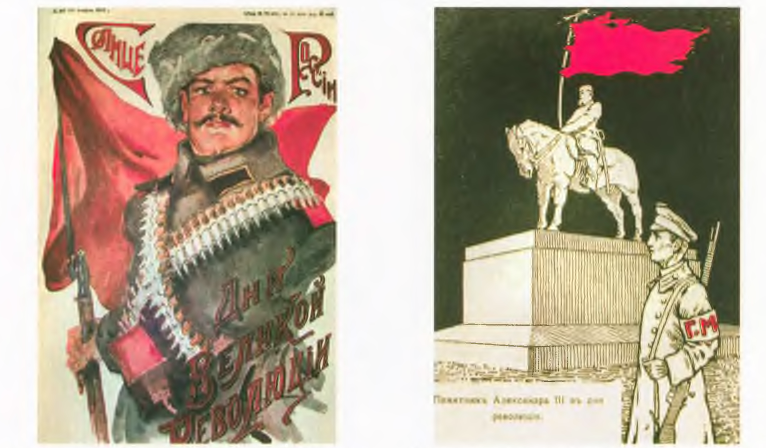
\includegraphics[width=148mm,height=140mm,keepaspectratio]{web/assets/i_001-source.png}\par{\small 原书图版：杂志士兵封面与骑马纪念像、市民袖标}\end{center}

\hypertarget{part2-4-b124}{}% part2-4-b124

\par\smallskip

\hypertarget{part2-4-b125}{}% part2-4-b125

\emph{杂志封面。封面上画着一名身穿沃伦近卫团制服的士兵。该团预备营于1917年2月27日起义。该团享有“第一个革命团”的声誉。}
\par


\hypertarget{part2-4-b126}{}% part2-4-b126

\emph{革命期间的亚历山大三世纪念碑。位于兹纳缅斯克广场的纪念碑被装饰上红旗，成为彼得格勒革命的象征之一。变化的另一个标志是佩戴市民治安队袖标的学生。明信片。1917年。}
\par


\hypertarget{part2-4-b127}{}% part2-4-b127

\par\smallskip

\hypertarget{part2-4-b128}{}% part2-4-b128

\needspace{120.5mm}\begin{center}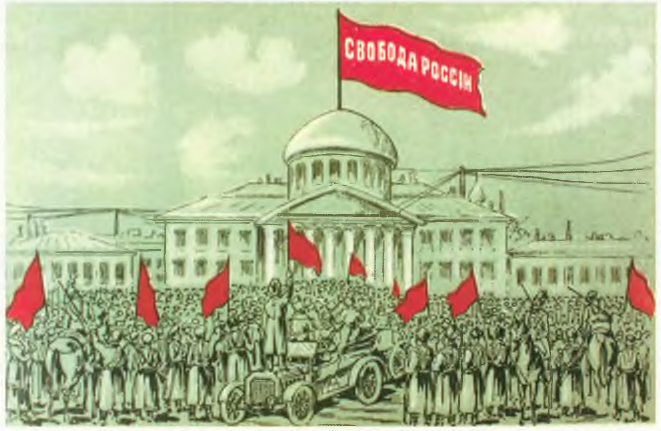
\includegraphics[width=148mm,height=140mm,keepaspectratio]{web/assets/i_002-source.png}\par{\small 原书图版：塔夫利达宫及夸张红旗}\end{center}

\hypertarget{part2-4-b129}{}% part2-4-b129

\par\smallskip

\hypertarget{part2-4-b130}{}% part2-4-b130

\emph{二月革命的象征之一，是绘有夸张巨大的红旗的塔夫利达宫图像。明信片。1917年。}
\par


\hypertarget{part2-4-b131}{}% part2-4-b131

\par\smallskip

\hypertarget{part2-4-b132}{}% part2-4-b132

\needspace{134.3mm}\begin{center}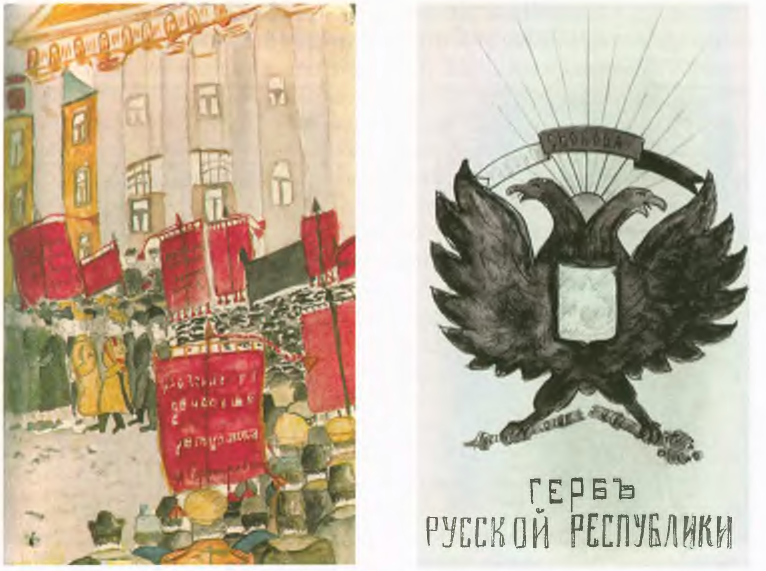
\includegraphics[width=148mm,height=140mm,keepaspectratio]{web/assets/i_003-source.png}\par{\small 原书图版：儿童画与共和国双头鹰国徽方案}\end{center}

\hypertarget{part2-4-b133}{}% part2-4-b133

\par\smallskip

\hypertarget{part2-4-b134}{}% part2-4-b134

\emph{儿童画。画中描绘1917年2月莫斯科的事件。1917年。}
\par


\hypertarget{part2-4-b135}{}% part2-4-b135

\emph{新国徽方案之一。1917年。}
\par


\hypertarget{part2-4-b136}{}% part2-4-b136

\par\smallskip

\hypertarget{part2-4-b137}{}% part2-4-b137

\needspace{124.3mm}\begin{center}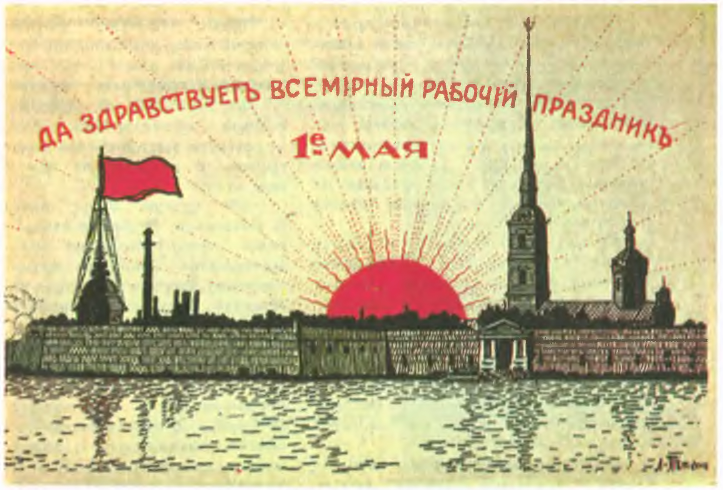
\includegraphics[width=148mm,height=140mm,keepaspectratio]{web/assets/i_004-source.png}\par{\small 原书图版：要塞、红旗与北方升起的太阳}\end{center}

\hypertarget{part2-4-b138}{}% part2-4-b138

\par\smallskip

\hypertarget{part2-4-b139}{}% part2-4-b139

\emph{彼得保罗要塞——昔日的“俄国巴士底狱”——被描绘成“新生活”的象征：要塞上空升起红旗，要塞上方升起“自由太阳”。按照画家的意愿，太阳从北方升起。明信片。1917年。}
\par


\hypertarget{part2-4-b140}{}% part2-4-b140

\needspace{205mm}\subsection{“民主化”的双头鹰}

\hypertarget{part2-4-b141}{}% part2-4-b141

\needspace{108.8mm}\begin{center}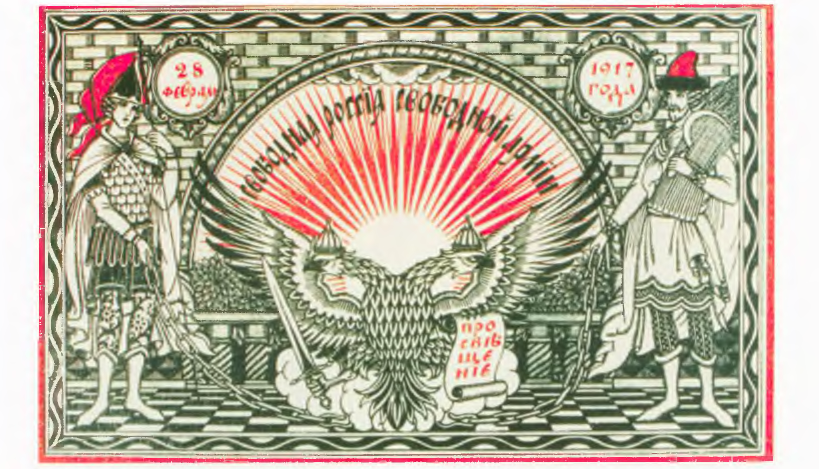
\includegraphics[width=148mm,height=140mm,keepaspectratio]{web/assets/i_005-source.png}\par{\small 原书图版：戴头盔双头鹰、剑、教育卷轴与红旗战士}\end{center}

\hypertarget{part2-4-b142}{}% part2-4-b142

\par\smallskip

\hypertarget{part2-4-b143}{}% part2-4-b143

\emph{明信片：“自由俄国致自由军队”。在画家笔下，被“自由太阳”照亮的双头鹰仍是俄国的国家象征。但皇冠被古代头盔取代，权杖和金球被剑与写有“教育”字样的卷轴取代。手持红旗的战士象征自由军队。}
\par


\hypertarget{part2-4-b144}{}% part2-4-b144

\par\smallskip

\hypertarget{part2-4-b145}{}% part2-4-b145

\needspace{96.8mm}\begin{center}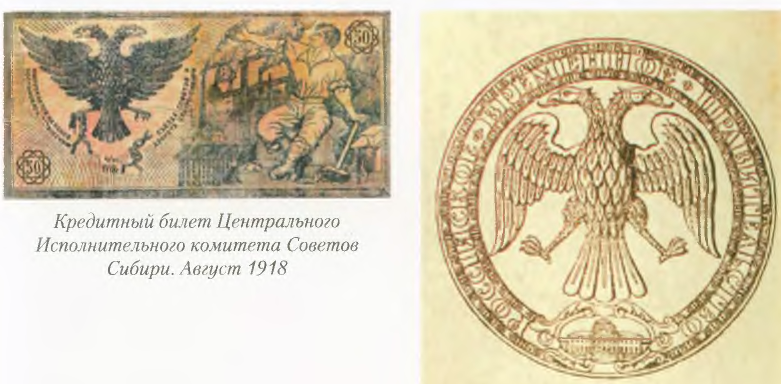
\includegraphics[width=148mm,height=140mm,keepaspectratio]{web/assets/i_006-source.png}\par{\small 原书图版：西伯利亚纸币与新国家印章}\end{center}

\hypertarget{part2-4-b146}{}% part2-4-b146

\par\smallskip

\hypertarget{part2-4-b147}{}% part2-4-b147

\emph{西伯利亚苏维埃中央执行委员会纸币。1918年8月。}
\par


\hypertarget{part2-4-b148}{}% part2-4-b148

\emph{新的俄罗斯国家印章。明信片。1917年。}
\par


\hypertarget{part2-4-b149}{}% part2-4-b149

\needspace{205mm}\subsection{作为“旧制度”象征的双头鹰}

\hypertarget{part2-4-b150}{}% part2-4-b150

\needspace{117.9mm}\begin{center}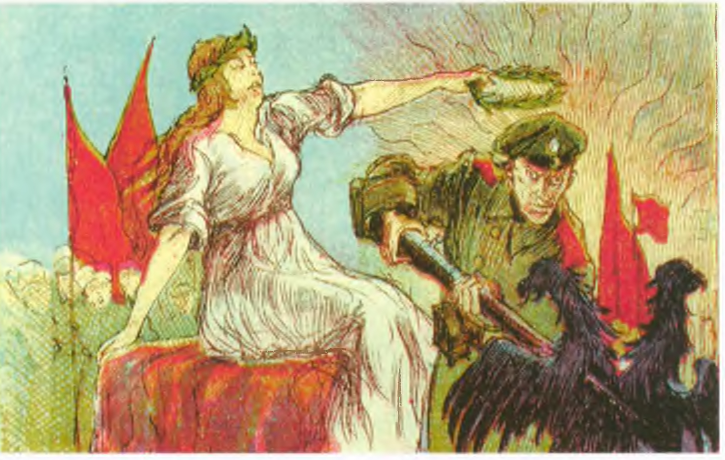
\includegraphics[width=148mm,height=140mm,keepaspectratio]{web/assets/i_007-source.png}\par{\small 原书图版：自由女神为毁鹰士兵加冠}\end{center}

\hypertarget{part2-4-b151}{}% part2-4-b151

\par\smallskip

\hypertarget{part2-4-b152}{}% part2-4-b152

\emph{“自由”把月桂花环戴在消灭双头鹰的俄国士兵头上。即使去掉皇冠也救不了双头鹰。明信片。1917年。}
\par


\hypertarget{part2-4-b153}{}% part2-4-b153

\par\smallskip

\hypertarget{part2-4-b154}{}% part2-4-b154

\needspace{123.5mm}\begin{center}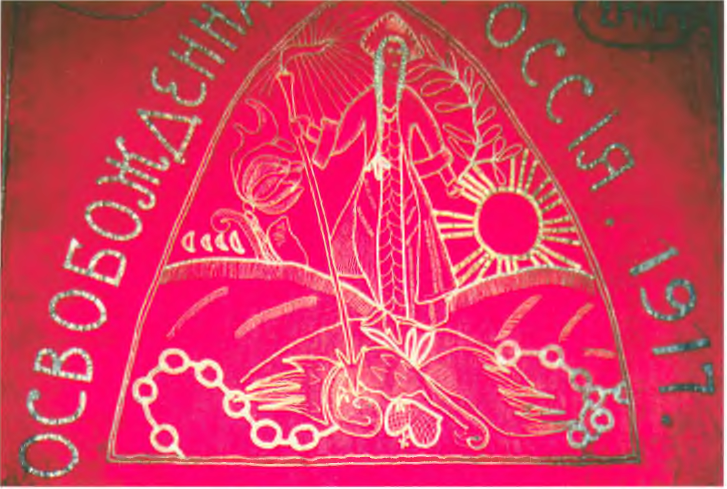
\includegraphics[width=148mm,height=140mm,keepaspectratio]{web/assets/i_008-source.png}\par{\small 原书图版：红旗上俄国女性寓意像踩鹰}\end{center}

\hypertarget{part2-4-b155}{}% part2-4-b155

\par\smallskip

\hypertarget{part2-4-b156}{}% part2-4-b156

\emph{部队的新军旗。身穿民族服装、象征“被解放的俄国”的妇女正在消灭双头鹰，这里的双头鹰体现“旧制度”。1917年。}
\par


\hypertarget{part2-4-b157}{}% part2-4-b157

\needspace{205mm}\subsection{革命条件下的旧象征与新象征}

\hypertarget{part2-4-b158}{}% part2-4-b158

\needspace{121.4mm}\begin{center}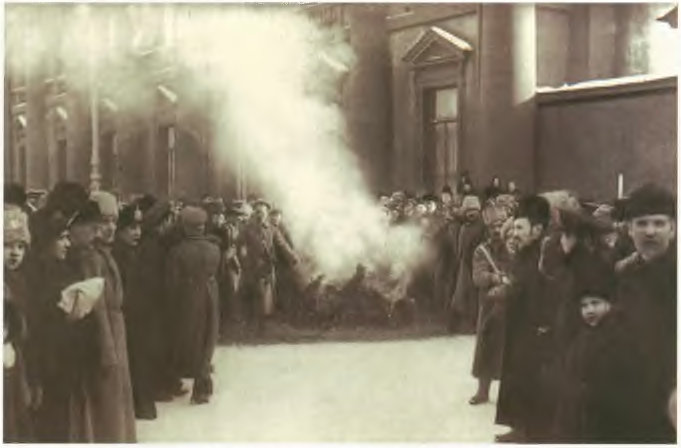
\includegraphics[width=148mm,height=140mm,keepaspectratio]{web/assets/i_009-source.png}\par{\small 原书图版：宫殿外焚烧徽记的照片}\end{center}

\hypertarget{part2-4-b159}{}% part2-4-b159

\par\smallskip

\hypertarget{part2-4-b160}{}% part2-4-b160

\emph{彼得格勒的二月革命。}
\par


\hypertarget{part2-4-b161}{}% part2-4-b161

\emph{阿尼奇科夫宫旁焚烧沙皇徽记。照片。1917年。}
\par


\hypertarget{part2-4-b162}{}% part2-4-b162

\par\smallskip

\hypertarget{part2-4-b163}{}% part2-4-b163

\needspace{129.2mm}\begin{center}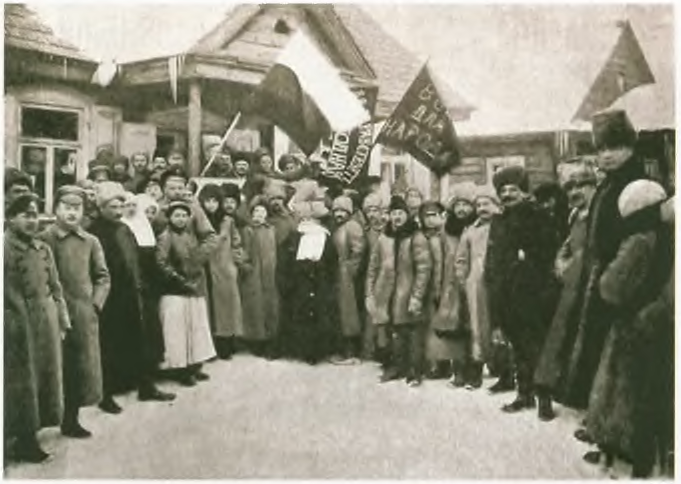
\includegraphics[width=148mm,height=140mm,keepaspectratio]{web/assets/i_010-source.png}\par{\small 原书图版：村镇群体举国旗及红旗照片}\end{center}

\hypertarget{part2-4-b164}{}% part2-4-b164

\par\smallskip

\hypertarget{part2-4-b165}{}% part2-4-b165

\emph{外省的“自由节日”。维尔纳省沃尔任镇的全俄地方自治联合会职员3月5日迎接新生活的曙光。《火花》（Искры）。1917年第12期（3月26日），第91页。国旗和红旗和平共处。照片。1917年。}
\par


\hypertarget{part2-4-b166}{}% part2-4-b166

\needspace{205mm}\subsection{“自由战士”崇拜}

\hypertarget{part2-4-b167}{}% part2-4-b167

\needspace{104.8mm}\begin{center}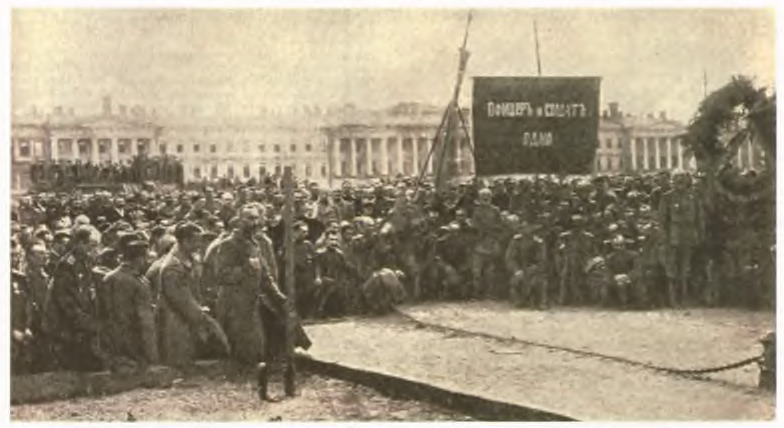
\includegraphics[width=148mm,height=140mm,keepaspectratio]{web/assets/i_011-source.png}\par{\small 原书图版：战神广场军人集会照片}\end{center}

\hypertarget{part2-4-b168}{}% part2-4-b168

\par\smallskip

\hypertarget{part2-4-b169}{}% part2-4-b169

\emph{全俄军官代表大会代表于1917年5月14日在战神广场游行。《火花》。1917年第20期（5月28日），第159页。1917年照片。}
\par


\hypertarget{part2-4-b170}{}% part2-4-b170

\par\smallskip

\hypertarget{part2-4-b171}{}% part2-4-b171

\needspace{130.1mm}\begin{center}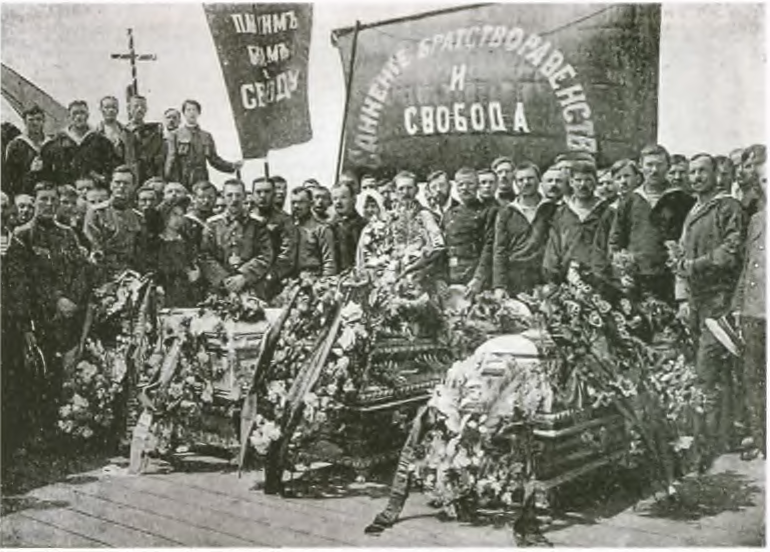
\includegraphics[width=148mm,height=140mm,keepaspectratio]{web/assets/i_012-source.png}\par{\small 原书图版：甲板上棺柩、军人与红旗}\end{center}

\hypertarget{part2-4-b172}{}% part2-4-b172

\par\smallskip

\hypertarget{part2-4-b173}{}% part2-4-b173

\emph{彼·彼·施密特中尉及其同志遗骸的迁葬。棺材停放在“玛丽亚公主”号巡洋舰甲板上。1917年。}
\par


\hypertarget{part2-4-b174}{}% part2-4-b174

\needspace{205mm}\subsection{革命象征与东正教会。喀琅施塔得。1917年}

\hypertarget{part2-4-b175}{}% part2-4-b175

\needspace{118.9mm}\begin{center}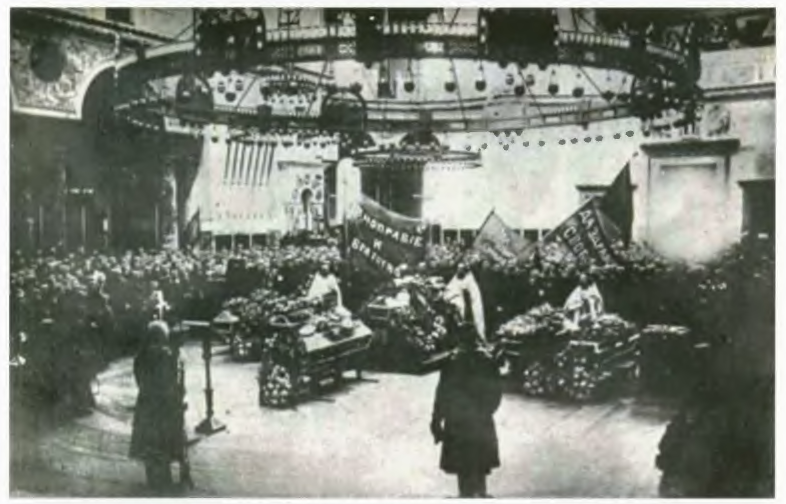
\includegraphics[width=148mm,height=140mm,keepaspectratio]{web/assets/i_013-source.png}\par{\small 原书图版：教堂内棺柩及红旗}\end{center}

\hypertarget{part2-4-b176}{}% part2-4-b176

\par\smallskip

\hypertarget{part2-4-b177}{}% part2-4-b177

\emph{在喀琅施塔得大教堂为二月革命中牺牲的水兵举行葬礼礼拜。红旗被抬进教堂。照片。1917年。}
\par


\hypertarget{part2-4-b178}{}% part2-4-b178

\par\smallskip

\hypertarget{part2-4-b179}{}% part2-4-b179

\needspace{164mm}\begin{center}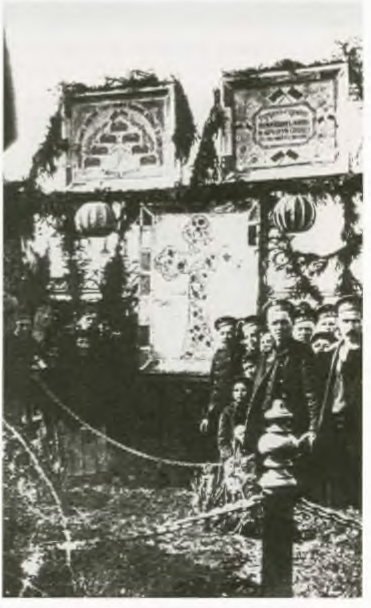
\includegraphics[width=148mm,height=140mm,keepaspectratio]{web/assets/i_014-source.png}\par{\small 原书图版：墓地、花环与宗教标志}\end{center}

\hypertarget{part2-4-b180}{}% part2-4-b180

\par\smallskip

\hypertarget{part2-4-b181}{}% part2-4-b181

\emph{二月革命中牺牲水兵之墓。喀琅施塔得。革命象征与宗教象征并存。照片。1917年。}
\par


\hypertarget{part2-4-b182}{}% part2-4-b182

\par\smallskip

\hypertarget{part2-4-b183}{}% part2-4-b183

\needspace{141.3mm}\begin{center}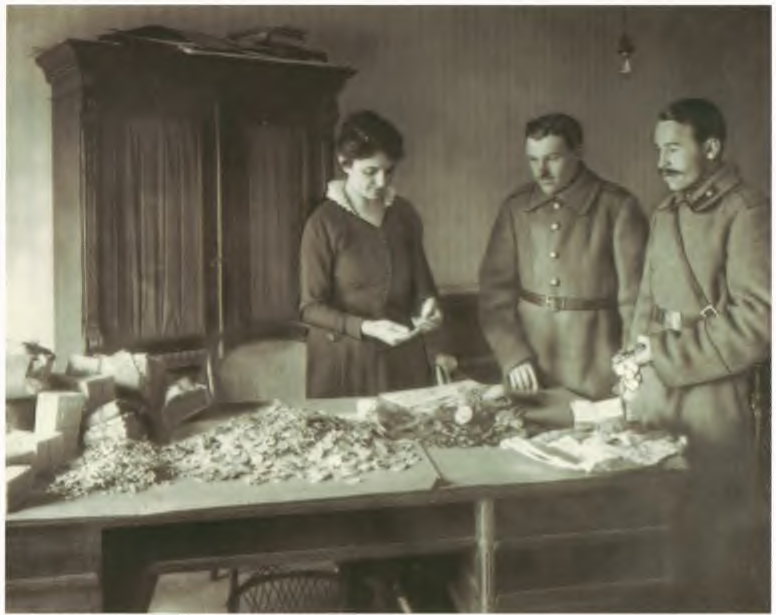
\includegraphics[width=148mm,height=140mm,keepaspectratio]{web/assets/i_015-source.png}\par{\small 原书图版：桌上勋章奖章、清点人员}\end{center}

\hypertarget{part2-4-b184}{}% part2-4-b184

\par\smallskip

\hypertarget{part2-4-b185}{}% part2-4-b185

\emph{彼得格勒苏维埃接收奖章和勋章。照片。1917年。}
\par


\hypertarget{part2-4-b186}{}% part2-4-b186

\par\smallskip

\hypertarget{part2-4-b187}{}% part2-4-b187

\needspace{117.9mm}\begin{center}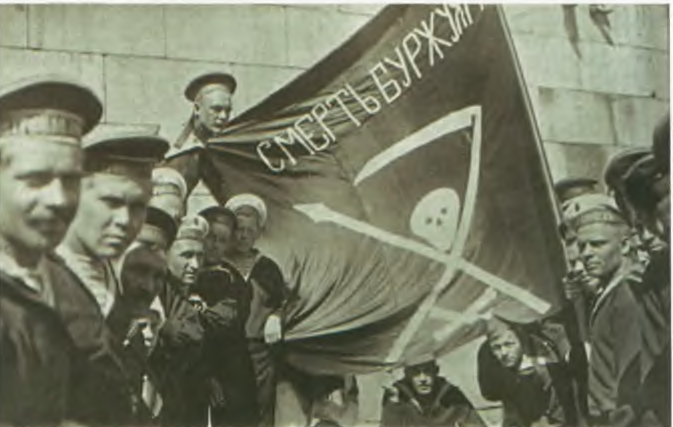
\includegraphics[width=148mm,height=140mm,keepaspectratio]{web/assets/i_016-source.png}\par{\small 原书图版：持死亡资产阶级横幅的水兵}\end{center}

\hypertarget{part2-4-b188}{}% part2-4-b188

\par\smallskip

\hypertarget{part2-4-b189}{}% part2-4-b189

\emph{“彼得罗巴甫洛夫斯克”号战列舰水兵在游行中。大多数海员衣着整洁，但制服并不统一。许多人摘下了无檐帽上的帽徽。照片。赫尔辛福斯。1917年夏。}
\par


\hypertarget{part2-4-b190}{}% part2-4-b190

\par\smallskip

\hypertarget{source-plate-185-h001}{}% source-plate-185-h001

\needspace{205mm}\subsection{革命象征与东正教会。1917年复活节}

\hypertarget{part2-4-b191}{}% part2-4-b191

\needspace{164mm}\begin{center}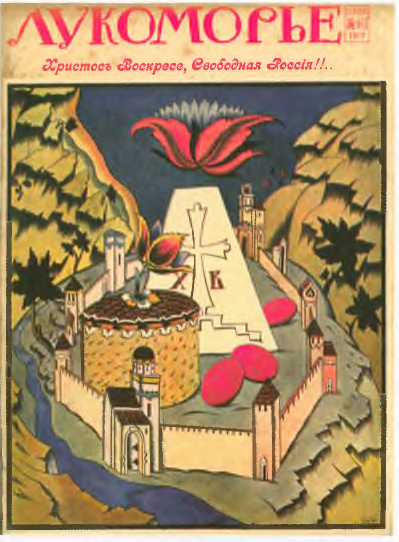
\includegraphics[width=148mm,height=140mm,keepaspectratio]{web/assets/i_017-source.png}\par{\small 原书图版：复活节号杂志彩色封面}\end{center}

\hypertarget{part2-4-b192}{}% part2-4-b192

\par\smallskip

\hypertarget{part2-4-b193}{}% part2-4-b193

\emph{画报复活节专号封面。1917年。}
\par


\hypertarget{part2-4-b194}{}% part2-4-b194

\par\smallskip

\hypertarget{part2-4-b195}{}% part2-4-b195

\needspace{130.5mm}\begin{center}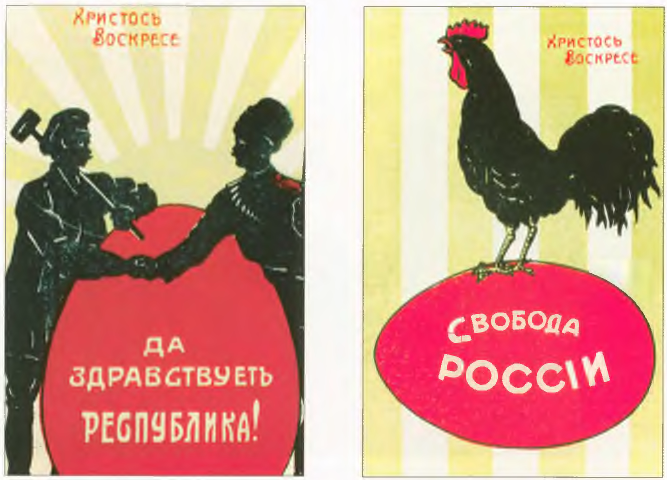
\includegraphics[width=148mm,height=140mm,keepaspectratio]{web/assets/i_018-source.png}\par{\small 原书图版：两幅复活节明信片、红蛋与共和口号}\end{center}

\hypertarget{part2-4-b196}{}% part2-4-b196

\par\smallskip

\hypertarget{part2-4-b197}{}% part2-4-b197

\emph{复活节明信片。1917年。}
\par


\hypertarget{part2-4-b198}{}% part2-4-b198

\par\smallskip

\hypertarget{part2-4-b199}{}% part2-4-b199

\needspace{164mm}\begin{center}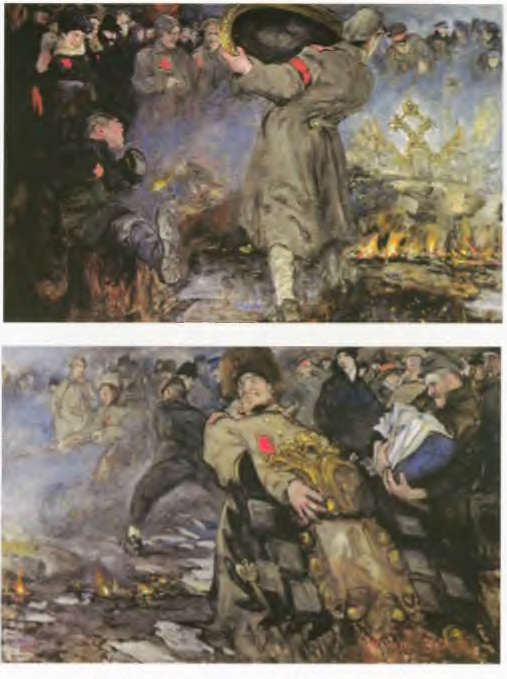
\includegraphics[width=148mm,height=140mm,keepaspectratio]{web/assets/i_019-source.png}\par{\small 原书图版：焚烧双头鹰画作两局部}\end{center}

\hypertarget{part2-4-b200}{}% part2-4-b200

\par\smallskip

\hypertarget{part2-4-b201}{}% part2-4-b201

\emph{阿·伊·瓦赫拉梅耶夫画作《焚烧双头鹰》（1917年）局部。}
\par


\hypertarget{part2-4-b202}{}% part2-4-b202

\par\smallskip

\hypertarget{part2-4-b203}{}% part2-4-b203

\needspace{131.3mm}\begin{center}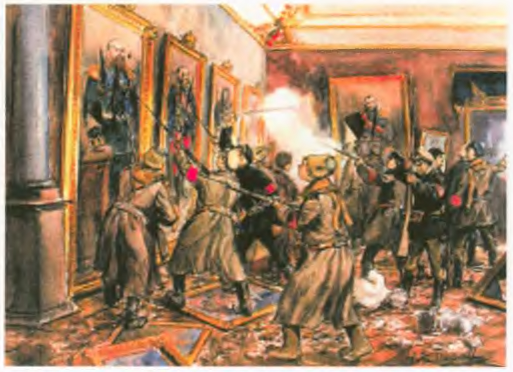
\includegraphics[width=148mm,height=140mm,keepaspectratio]{web/assets/i_020-source.png}\par{\small 原书图版：士兵在宫殿内毁像画作}\end{center}

\hypertarget{part2-4-b204}{}% part2-4-b204

\par\smallskip

\hypertarget{part2-4-b205}{}% part2-4-b205

\emph{伊·弗·弗拉基米罗夫画作（1918年？）。}
\par


\hypertarget{part2-4-b206}{}% part2-4-b206

\needspace{205mm}\subsection{1917年春天红旗的政治利用}

\hypertarget{part2-4-b207}{}% part2-4-b207

\needspace{123.9mm}\begin{center}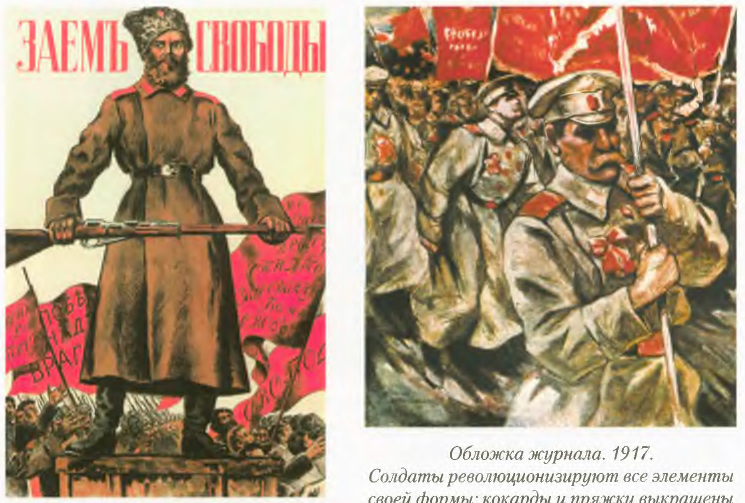
\includegraphics[width=148mm,height=140mm,keepaspectratio]{web/assets/i_021-source.png}\par{\small 原书图版：自由公债海报与军人红色服饰杂志封面}\end{center}

\hypertarget{part2-4-b208}{}% part2-4-b208

\par\smallskip

\hypertarget{part2-4-b209}{}% part2-4-b209

\emph{“自由公债”。鲍·米·库斯托季耶夫宣传画。1917年。}
\par


\hypertarget{part2-4-b210}{}% part2-4-b210

\emph{杂志封面。1917年。士兵们把自己制服的所有部件都革命化：帽徽和带扣被涂成红色或用红布包裹。}
\par


\hypertarget{part2-4-b211}{}% part2-4-b211

\par\smallskip

\hypertarget{part2-4-b212}{}% part2-4-b212

\needspace{120.2mm}\begin{center}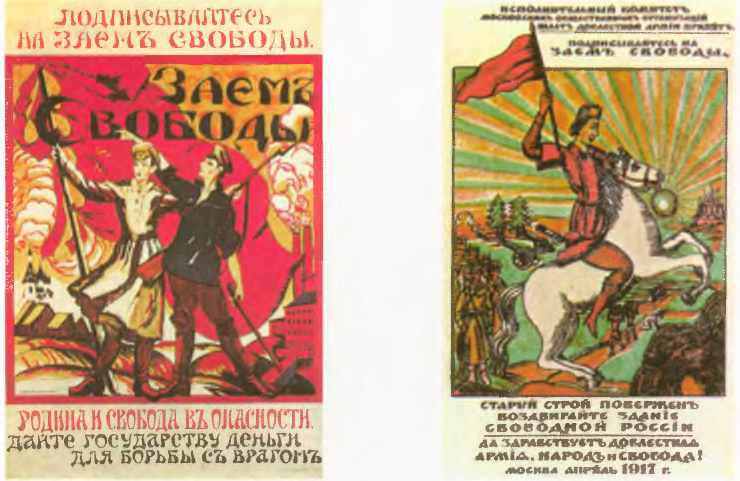
\includegraphics[width=148mm,height=140mm,keepaspectratio]{web/assets/i_022-source.png}\par{\small 原书图版：两幅自由公债宣传明信片}\end{center}

\hypertarget{part2-4-b213}{}% part2-4-b213

\par\smallskip

\hypertarget{part2-4-b214}{}% part2-4-b214

\emph{“自由公债”。阿·伊·克拉夫琴科明信片。1917年。}
\par


\hypertarget{part2-4-b215}{}% part2-4-b215

\emph{“自由公债”。彼·库兹涅佐夫明信片。1917年。}
\par


\hypertarget{part2-4-b216}{}% part2-4-b216

\needspace{205mm}\subsection{大众文化中的革命象征}

\hypertarget{part2-4-b217}{}% part2-4-b217

\needspace{117.9mm}\begin{center}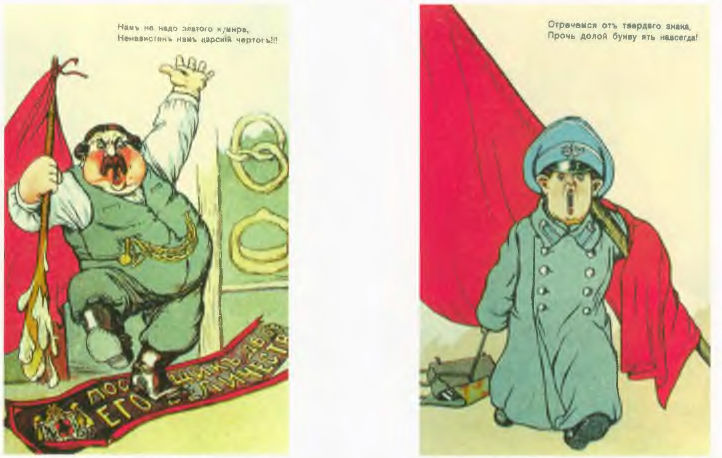
\includegraphics[width=148mm,height=140mm,keepaspectratio]{web/assets/i_023-source.png}\par{\small 原书图版：面包商踩旧招牌与正字法改革中学生两幅漫画}\end{center}

\hypertarget{part2-4-b218}{}% part2-4-b218

\par\smallskip

\hypertarget{part2-4-b219}{}% part2-4-b219

\emph{明信片（1917年）。明信片“我们不需要黄金偶像，沙皇的宫殿令我们憎恶！”。一位事业有成的面包师——昔日皇室供应商——象征那个时代的政治机会主义。他在红旗下高唱《工人马赛曲》，践踏自己的招牌。}
\par


\hypertarget{part2-4-b220}{}% part2-4-b220

\emph{明信片：“让我们抛弃硬音符（ъ），滚开，永远废除字母‘雅特’（ять，ѣ）！”手持红旗、改写《工人马赛曲》歌词的中学生象征反对“旧正字法”的斗争。正字法改革由临时政府实施，在社会上引起很大争论。后来，“旧”字母变成了政治象征。}
\par


\hypertarget{part2-4-b221}{}% part2-4-b221

\par\smallskip

\hypertarget{part2-4-b222}{}% part2-4-b222

\needspace{133.5mm}\begin{center}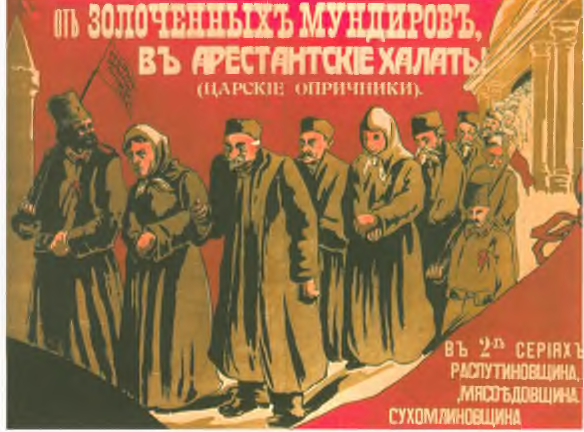
\includegraphics[width=148mm,height=140mm,keepaspectratio]{web/assets/i_024-source.png}\par{\small 原书图版：从金饰军服到囚服电影海报}\end{center}

\hypertarget{part2-4-b223}{}% part2-4-b223

\par\smallskip

\hypertarget{part2-4-b224}{}% part2-4-b224

\emph{电影海报。1917年。}
\par


\hypertarget{part2-4-b225}{}% part2-4-b225

\needspace{205mm}\subsection{革命与海军制服}

\hypertarget{part2-4-b226}{}% part2-4-b226

\needspace{135.5mm}\begin{center}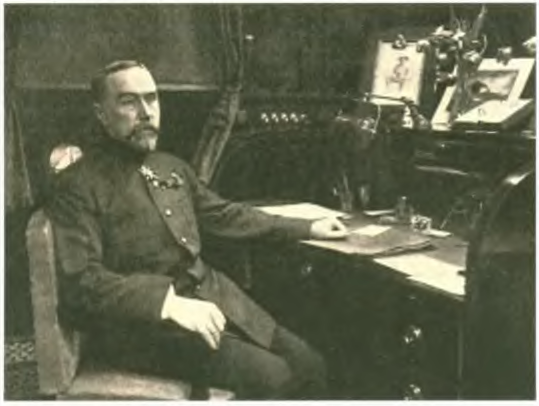
\includegraphics[width=148mm,height=140mm,keepaspectratio]{web/assets/i_025-source.png}\par{\small 原书图版：马克西莫夫桌前无肩章照}\end{center}

\hypertarget{part2-4-b227}{}% part2-4-b227

\par\smallskip

\hypertarget{part2-4-b228}{}% part2-4-b228

\emph{波罗的海舰队司令、海军中将亚·谢·马克西莫夫。这位将领没有佩戴其军衔的区别标志，他的制服上衣装饰着勋章和红蝴蝶结。照片。1917年4月。}
\par


\hypertarget{part2-4-b229}{}% part2-4-b229

\par\smallskip

\hypertarget{part2-4-b230}{}% part2-4-b230

\needspace{145.1mm}\begin{center}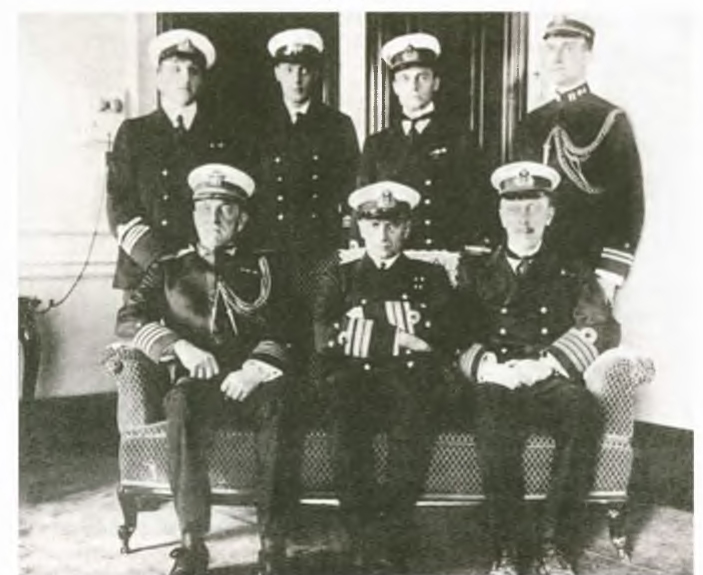
\includegraphics[width=148mm,height=140mm,keepaspectratio]{web/assets/i_026-source.png}\par{\small 原书图版：海军军官组照、新旧袖标军服}\end{center}

\hypertarget{part2-4-b231}{}% part2-4-b231

\par\smallskip

\hypertarget{part2-4-b232}{}% part2-4-b232

\emph{由海军将领亚·瓦·高尔察克带领的一群俄国海军军官在纽约。照片。1917年。}
\par


\hypertarget{part2-4-b233}{}% part2-4-b233

\needspace{205mm}\subsection{革命与服装}

\hypertarget{part2-4-b234}{}% part2-4-b234

\needspace{132.0mm}\begin{center}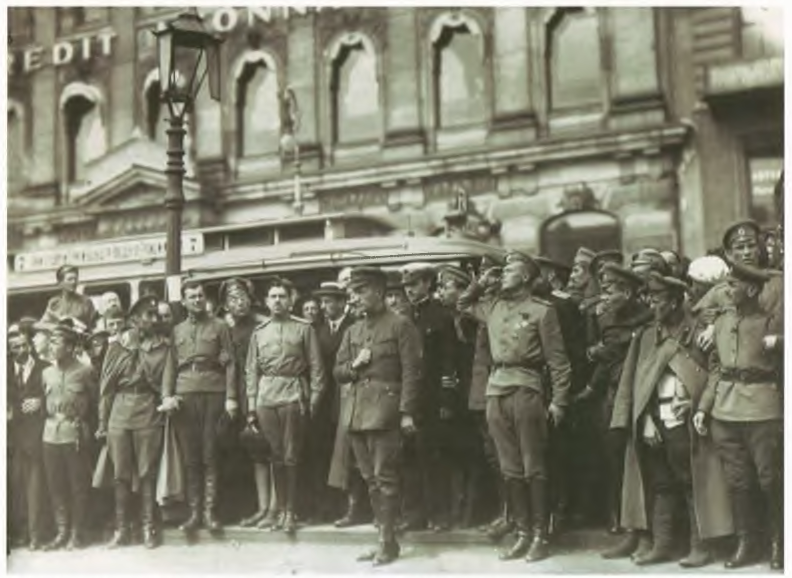
\includegraphics[width=148mm,height=140mm,keepaspectratio]{web/assets/i_027-source.png}\par{\small 原书图版：克伦斯基等人葬礼街头照片}\end{center}

\hypertarget{part2-4-b235}{}% part2-4-b235

\par\smallskip

\hypertarget{part2-4-b236}{}% part2-4-b236

\emph{七月事变中牺牲的哥萨克的隆重葬礼。彼得格勒，1917年7月15日，照片。亚·费·克伦斯基身后站着他的海军副官，后者即使在这样的仪式上也不敢穿夏季制服。离军事部长几步远的军人并不注意遵守着装规定。}
\par


\hypertarget{part2-4-b237}{}% part2-4-b237

\par\smallskip

\hypertarget{part2-4-b238}{}% part2-4-b238

\needspace{114.5mm}\begin{center}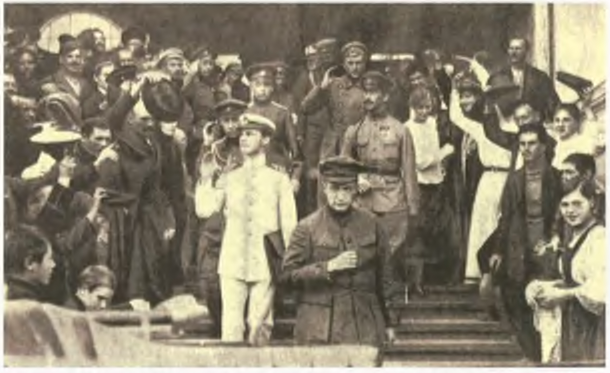
\includegraphics[width=148mm,height=140mm,keepaspectratio]{web/assets/i_028-source.png}\par{\small 原书图版：国务会议台阶、夏季白制服副官}\end{center}

\hypertarget{part2-4-b239}{}% part2-4-b239

\par\smallskip

\hypertarget{part2-4-b240}{}% part2-4-b240

\emph{莫斯科国务会议（1917年8月）。照片。亚·费·克伦斯基的海军副官身穿新夏季制服。}
\par


\hypertarget{part2-4-b241}{}% part2-4-b241

\needspace{205mm}\subsection{武装力量中的革命时尚}

\hypertarget{part2-4-b242}{}% part2-4-b242

\needspace{100.5mm}\begin{center}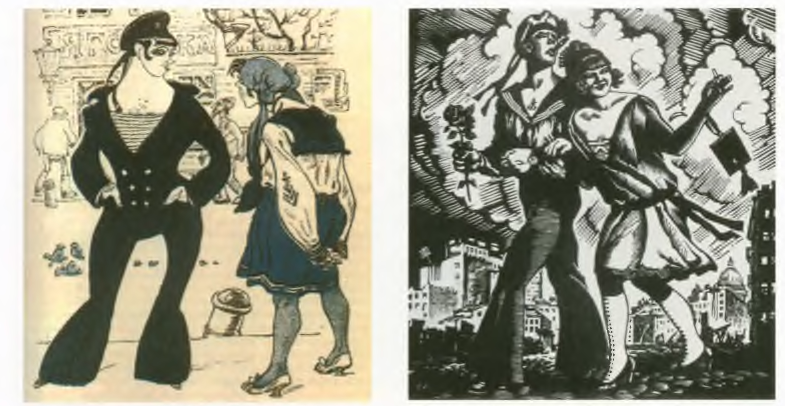
\includegraphics[width=148mm,height=140mm,keepaspectratio]{web/assets/i_029-source.png}\par{\small 原书图版：漫画与水兵情侣油毡版画}\end{center}

\hypertarget{part2-4-b243}{}% part2-4-b243

\par\smallskip

\hypertarget{part2-4-b244}{}% part2-4-b244

\emph{雷米（尼·瓦·列米佐夫）的漫画。《新萨蒂里孔》第37期。1917年。}
\par


\hypertarget{part2-4-b245}{}% part2-4-b245

\emph{鲍·米·库斯托季耶夫。《水兵与心爱的人》。油毡版画。1926年。}
\par


\hypertarget{part2-4-b246}{}% part2-4-b246

\par\smallskip

\hypertarget{part2-4-b247}{}% part2-4-b247

\needspace{133.8mm}\begin{center}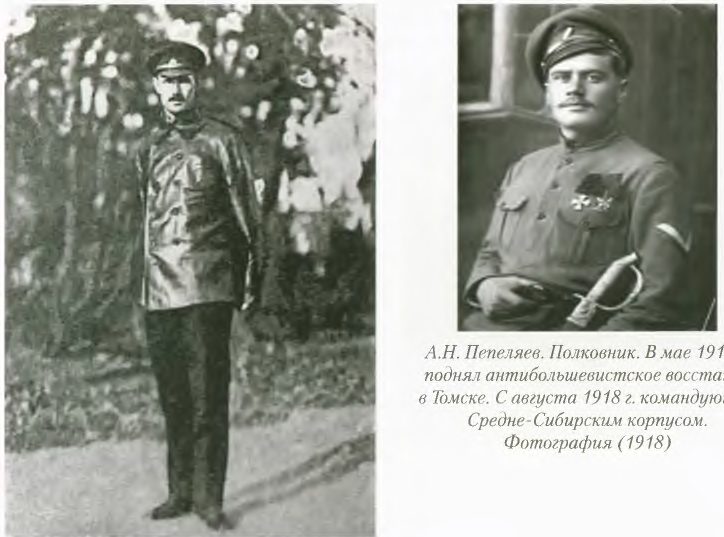
\includegraphics[width=148mm,height=140mm,keepaspectratio]{web/assets/i_030-source.png}\par{\small 原书图版：斯坦克维奇与佩佩利亚耶夫两照片}\end{center}

\hypertarget{part2-4-b248}{}% part2-4-b248

\par\smallskip

\hypertarget{part2-4-b249}{}% part2-4-b249

\emph{弗·鲍·斯坦克维奇。少尉，临时政府驻北方面军总司令处专员。照片（1917年）。}
\par


\hypertarget{part2-4-b250}{}% part2-4-b250

\emph{阿·尼·佩佩利亚耶夫。上校。1918年5月在托木斯克发动反布尔什维克起义。1918年8月起任中西伯利亚军军长。照片（1918年）。}
\par


\hypertarget{part2-4-b251}{}% part2-4-b251

\needspace{205mm}\subsection{武装力量中的红旗}

\hypertarget{part2-4-b252}{}% part2-4-b252

\needspace{112.3mm}\begin{center}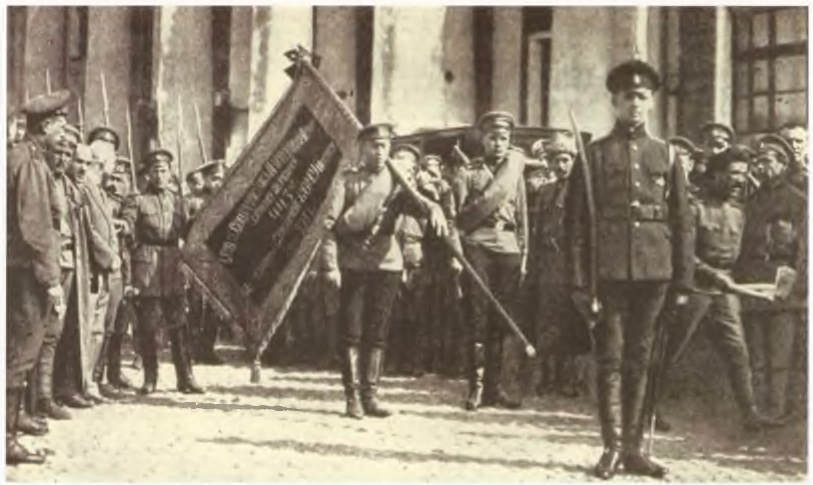
\includegraphics[width=148mm,height=140mm,keepaspectratio]{web/assets/i_031-source.png}\par{\small 原书图版：仪仗军旗移交照片}\end{center}

\hypertarget{part2-4-b253}{}% part2-4-b253

\par\smallskip

\hypertarget{part2-4-b254}{}% part2-4-b254

\emph{人民军队社会主义者联盟的军旗被授予仪仗队，以便转交第443索斯宁团，1917年5月20日。照片。彼得格勒军区司令彼·阿·波洛夫佐夫将军参加了仪式并发表隆重讲话。}
\par


\hypertarget{part2-4-b255}{}% part2-4-b255

\par\smallskip

\hypertarget{part2-4-b256}{}% part2-4-b256

\needspace{121.9mm}\begin{center}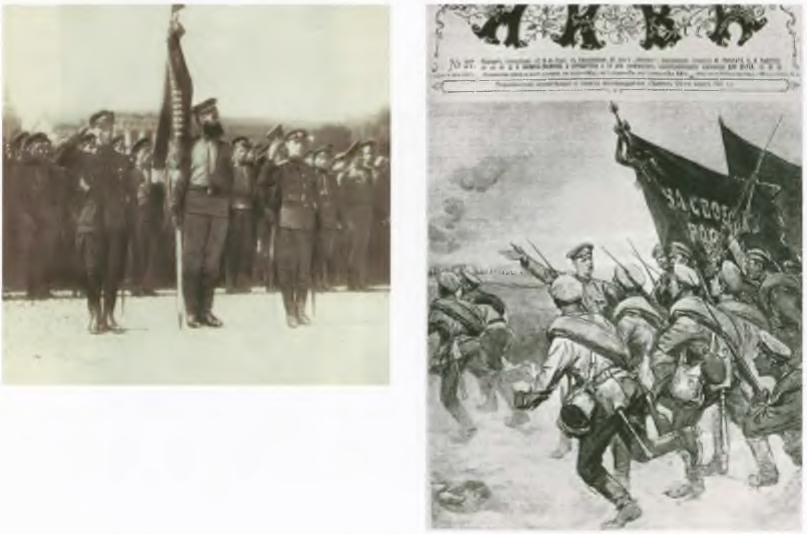
\includegraphics[width=148mm,height=140mm,keepaspectratio]{web/assets/i_032-source.png}\par{\small 原书图版：军旗列队照片与Нива封面}\end{center}

\hypertarget{part2-4-b257}{}% part2-4-b257

\par\smallskip

\hypertarget{part2-4-b258}{}% part2-4-b258

\emph{献给六月攻势的《田地》杂志封面。}
\par


\hypertarget{part2-4-b259}{}% part2-4-b259

\par\smallskip

\hypertarget{part2-4-b260}{}% part2-4-b260

这道命令的出台，是由陆军中反对肩章的运动引起的；看来，在舰队命令颁布之后，这场运动更加激烈了：“与此同时，已经出现的情况不仅是擅自废除肩章，甚至还有从军官身上强行扯下肩章的事。我警告，我不允许军队中出现此类擅自行动和暴力，并将对犯有此类行为者追究最严厉的责任。我命令陆军及陆军事务部门的全体军官和士兵，严格而准确地遵守一切现行且未被废除的服装规定”\nobreak\hypertarget{ref-n_600-zh}{}\hyperlink{note-n_600-zh}{\textsuperscript{333}}。可以确信，这道命令的出现与将军圈子中极为严重的担忧有关。陆军中围绕肩章的冲突，在他们看来完全是现实的前景。
\par


\hypertarget{part2-4-b261}{}% part2-4-b261

某些海军部门部队的军人身着陆军制服，他们也应保留肩章。海军参谋本部4月19日的电报称：“关于服装的命令仅适用于海军制服。至于那些穿着陆军式样衣服的人，以及在陆军地区的人，则应与陆军人员一样穿着保护色制服”\nobreak\hypertarget{ref-n_601-zh}{}\hyperlink{note-n_601-zh}{\textsuperscript{334}}。
\par


\hypertarget{part2-4-b262}{}% part2-4-b262

海军军官的制服后来被称为“克伦斯基制服”，以纪念五月初就任军事与海军部长的新部长，尽管它还是在古契科夫任内引入的。人们对此态度不一——一些海军军官甚至试图辞职以示抗议，愤慨的老兵们给舰队指挥部写来批评信。海军武备学校的学员们早已梦想戴上金色肩章，他们把这道命令的消息视为令人悲伤的噩耗\nobreak\hypertarget{ref-n_602-zh}{}\hyperlink{note-n_602-zh}{\textsuperscript{335}}。军官们还害怕不少意外开支：据一位舰上财务稽核官计算，每位军官至少需要120卢布来改制所有规定应备的成套军服。而领导海军军官服装修订特别委员会的海军少将尼·尼·科洛梅伊佐夫甚至认为，为此应向每位军官提供200卢布的一次性贷款。军官们担心新的开支，请求在战争结束前禁止采用新制服。6月7日，海军参谋本部发布通令解释：“在战争结束前，不会对服装作任何引起开支的改动”\nobreak\hypertarget{ref-n_603-zh}{}\hyperlink{note-n_603-zh}{\textsuperscript{336}}。
\par


\hypertarget{part2-4-b263}{}% part2-4-b263

但许多人喜欢这些新事物。年轻军官很快置办了英式新军帽和刺绣帽徽。甚至有人说，驱逐舰“诺维克”号舰长曾对自己的军官们宣称：“革命至少为我们做了一件好事：我们再也不用像那些该死的陆军军官那样戴肩章了”\nobreak\hypertarget{ref-n_604-zh}{}\hyperlink{note-n_604-zh}{\textsuperscript{337}}。
\par


\hypertarget{part2-4-b264}{}% part2-4-b264

海军军人传统的亲英情结也起了作用：袖部饰带是英国海军的识别标志。一些海军将领早在革命前就提议对俄国海军制服作相应改动。不过，军官们有时不满于饰带的尺寸和数量与“经典”英国样式不同：例如，俄国海军上校得到的制服类似英国海军中校。一些军官建议更精确地复制英国制服。海军中校弗·伊·鲁德涅夫写道：“还有什么更简单的呢，采纳英国制度吧，它是国际性的，而且完全明确。……最重要的是，不要自作聪明，把英国人的一切都拿来，他们的制服确实高明。”然而，进一步改革识别标志已不可能。“目前不能对服装作任何其他改动和补充，因为任何改动都无法实现，除了有害的刺激之外，什么也不会引起，”海军军官服装修订委员会的一位成员5月24日在致委员会主席的信中恰如其分地指出\nobreak\hypertarget{ref-n_605-zh}{}\hyperlink{note-n_605-zh}{\textsuperscript{338}}。
\par


\hypertarget{part2-4-b265}{}% part2-4-b265

一些水兵对废除肩章漠不关心，甚至带着讽刺：在他们看来，更换制服是在偷换舰队和国家真正的变革。但对大多数普通水兵来说，取消肩章成了新制度重要的象征性胜利。一首由赫尔辛福斯水兵活动家写成的朴实诗作中，主人公感叹道：
\par


\hypertarget{part2-4-b266}{}% part2-4-b266

\begin{readingquote}
\par\needspace{5\baselineskip}
我也曾佩戴漂亮的肩章，\\*
但它让我厌烦透顶，\\*
肩章上曾有个危险的标记，\\*
肩章如今已彻底覆灭\nobreak\hypertarget{ref-n_606-zh}{}\hyperlink{note-n_606-zh}{\textsuperscript{339}}。
\end{readingquote}
\par


\hypertarget{part2-4-b267}{}% part2-4-b267

在其他舰队，摘下肩章也不只是简单的更换制服——人们把它视为新时代来临的标志。正在遥远的香港修理的“佩琴加”号船上一名水兵回忆道：“所有水兵都高兴地扯下自己的肩章，有的扔进海里，有的扔进锅炉炉膛”\nobreak\hypertarget{ref-n_607-zh}{}\hyperlink{note-n_607-zh}{\textsuperscript{340}}。
\par


\hypertarget{part2-4-b268}{}% part2-4-b268

古契科夫的命令把“肩章革命”进程中已经发展起来的过程固定下来，为这一阶段重要的象征冲突划上句号。但这些命令也引发了新的冲突，制造了新的问题。舰队废除肩章，再次使敬礼问题急剧尖锐化。海军指挥部被迫再次让步，实际上无视了最高统帅的命令。4月18日，海军部长助理、海军少将米·阿·克德罗夫“为执行和处置”发出电报：“在岸上非队列场合，废除敬礼。军人相遇时可以相互举手触帽致意。这种相互致意并非义务，完全取决于相遇者的善意和分寸。”4月20日，黑海舰队司令、海军中将亚·瓦·高尔察克又把非队列场合废除敬礼的规定扩大到相对“安定”（从指挥部角度看）的塞瓦斯托波尔的陆军事务部门人员\nobreak\hypertarget{ref-n_608-zh}{}\hyperlink{note-n_608-zh}{\textsuperscript{341}}。
\par


\hypertarget{part2-4-b269}{}% part2-4-b269

水兵们同样把废除肩章视为深化象征性变革的信号，并积极着手革命“军服创制”的新阶段。海军军官和海军部门制服新式样制定委员会委员、海军少将奥·奥·里希特给海军参谋本部写道：“在赫尔辛福斯，舰队里开始有人议论，新的军官制服上金子太多了……最好把军官制服简化一下。”在当前形势下，许多军官也不急于置办新制服：“在赫尔辛福斯，很少有人给自己缝上饰带。”就连海军将领亚·谢·马克西莫夫也没有执行自己的命令，穿着没有饰带的制服：“只有脖子上的弗拉基米尔勋章还能多少表明他属于军官阶层。”的确，在1917年拍摄的一张正式肖像照片上，以“革命海军将领”名声自豪的马克西莫夫身穿没有任何识别标志的海军制服上衣，但佩戴勋章和红蝴蝶结。波罗的海舰队主要基地的水兵继续使自己的制服革命化。“赫尔辛福斯不大听谁的话，因此他们可能自己给自己设计制服，”里希特写道。例如，船员们干脆摘掉帽徽，有些人则用白色金属制小锚代替帽徽，这使他们更像民用船队的水手\nobreak\hypertarget{ref-n_609-zh}{}\hyperlink{note-n_609-zh}{\textsuperscript{342}}。
\par


\hypertarget{part2-4-b270}{}% part2-4-b270

革命时尚发展起来，征服了各舰队。如果说在陆军中，革命化的标志之一是身穿无肩章的新军便服上衣、头戴带军官帽徽的大檐帽的逃兵形象，那么在舰队中，革命的成果则是宽大无比的喇叭裤。水兵们穿制服上衣时常常卷起袖子，不穿海魂衫，事件的同时代人回忆起“袒胸露颈”的水兵。正是这种革命水兵——“革命的光彩与骄傲”——的形象，被鲍·米·库斯托季耶夫和伊·阿·弗拉基米罗夫留在画布上。对作家苔菲来说，“光着胸膛、留着蝴蝶式额发的水兵”也成为新生活的象征之一\nobreak\hypertarget{ref-n_610-zh}{}\hyperlink{note-n_610-zh}{\textsuperscript{343}}。一位海军军官回忆道：“有了钱以后，水兵们首先开始打扮起来。出现了高筒漆皮靴，甚至只是带镜面般靴筒的胶皮靴；掐腰的短呢外套，钉着骑兵式纽扣；紧身的法兰绒衬衫，下摆露在外面；军帽歪戴着，夏天甚至戴草帽……头发特别受重视，剪发简直被认为不成体统。最时髦的是额前留起高高的额发，把胡子神气地卷起来”\nobreak\hypertarget{ref-n_611-zh}{}\hyperlink{note-n_611-zh}{\textsuperscript{344}}。
\par


\hypertarget{part2-4-b271}{}% part2-4-b271

也许可以设想，这位观念相当保守的军官回忆录作者在描绘神气的“弟兄们”时故意渲染，但一些波罗的海水兵也在回忆录中留下了战友的生动肖像，他们晚上去城里跳舞，想打动芬兰和爱沙尼亚姑娘：“他穿着黑色漆皮鞋和熨得笔挺的宽大喇叭裤，活像一只腿上羽毛蓬乱的老公鸡，裤脚像扫帚一样扫着街上的尘土”\nobreak\hypertarget{ref-n_612-zh}{}\hyperlink{note-n_612-zh}{\textsuperscript{345}}。
\par


\hypertarget{part2-4-b272}{}% part2-4-b272

但为寻找新制服操心的不只是波罗的海水兵。黑海舰队司令8月11日的命令反映了那里正在形成的局面：“从舰上上岸或从岸上部队外出的人员穿着五花八门，往往极其散漫，甚至肮脏。……尤其不能容忍把制服与便服混穿，军事部长的命令已予禁止。”这道命令被塞瓦斯托波尔苏维埃的报纸转载，但发表得相当晚——直到9月30日。可以推测，各委员会成员对命令态度不一，但相当一部分黑海水兵赞成它。9月3日，报上出现了巡洋舰“普鲁特”号水兵的决议。他们谴责“不伦不类、非便非军”的换装，呼吁其他水兵按规定着装——“毕竟没有比我们的军服更漂亮的衣服了”（他们从许多平民借用海军制服元素这一点上看到了佐证）。巡洋舰水兵还反感“社交界”时兴的马鞭，尤其反感“弟兄们”往手指上套“几乎几十个”宝石戒指和指环的做派\nobreak\hypertarget{ref-n_613-zh}{}\hyperlink{note-n_613-zh}{\textsuperscript{346}}。
\par


\hypertarget{part2-4-b273}{}% part2-4-b273

海军军人的外表不仅令指挥部和某些舰艇上的舰员感到震惊，也令民选海军组织的积极分子感到震惊。波罗的海舰队中央委员会要求水兵不要在无檐帽上佩戴写有他舰名称的帽带，这一呼吁已通过波罗的海舰队各编队的命令宣布\nobreak\hypertarget{ref-n_614-zh}{}\hyperlink{note-n_614-zh}{\textsuperscript{347}}。可以推测，水兵们或者不愿在休假（尤其是擅自离舰）时被认出，或者想分享那些以战斗或革命历史闻名的舰艇船员的荣耀。布尔什维克帕·叶·德边科本人就是一个著名例子：他是“夏”（Ща）号运输舰水兵，后来成为波罗的海舰队中央委员会主席。他戴的无檐帽帽带上赫然写着“Петропавлоск”（！），把“彼得罗巴甫洛夫斯克”号的俄文舰名“Петропавловск”拼错了——这顶帽子保存在中央海军博物馆\nobreak\hypertarget{ref-n_615-zh}{}\hyperlink{note-n_615-zh}{\textsuperscript{348}}。拼写错误表明，这条帽带是手工制作的。不过，佩戴写有流行舰名的帽带的时尚在随后几年仍然保持。例如，彼得格勒军港的布尔什维克政委伊·德·斯拉德科夫，就在无檐帽上戴着一条写有“奥列格”的圣乔治帽带，尽管他从未在该巡洋舰上服役\nobreak\hypertarget{ref-n_616-zh}{}\hyperlink{note-n_616-zh}{\textsuperscript{349}}。水兵活动家试图以此巩固自己的威望。有时，更换帽带还被用于宣传目的。例如，“布尔什维克”巡洋舰“金刚石”号的水兵在敖德萨卫戍区乌克兰部队士兵中进行鼓动时，为伪装起见戴上了“乌克兰化”巡洋舰“水星纪念”号的帽带\nobreak\hypertarget{ref-n_617-zh}{}\hyperlink{note-n_617-zh}{\textsuperscript{350}}。在某些情况下，水兵们把黑色帽带换成红色帽带\nobreak\hypertarget{ref-n_618-zh}{}\hyperlink{note-n_618-zh}{\textsuperscript{351}}。看来，这在1917年获得革命新名称的舰艇上尤为普遍。中央海军博物馆藏品中保存着写有巡洋舰“留里克”号和驱逐舰“自由”号名称的红色帽带\nobreak\hypertarget{ref-n_619-zh}{}\hyperlink{note-n_619-zh}{\textsuperscript{352}}。
\par


\hypertarget{part2-4-b274}{}% part2-4-b274

9月4日，全俄海军中央委员会（Центрофлот）通过了一项引人注目的决议，随后在海军部门命令中公布（波罗的海舰队的命令错误地称这一呼吁来自波罗的海舰队中央委员会）：“近来在街头和其他公共场所，舰队人员中可以看到十足的化装舞会，任意穿戴制服，往往发展到离奇的装束，有时很难判断这是水兵、半平民还是半士兵。”全俄海军中央委员会呼吁“制止进一步的化装舞会”，并要求遵守海军部长的命令\nobreak\hypertarget{ref-n_620-zh}{}\hyperlink{note-n_620-zh}{\textsuperscript{353}}。
\par


\hypertarget{part2-4-b275}{}% part2-4-b275

这类呼吁无法阻止革命时尚的胜利进军。一名水兵写的讽刺诗，让人可以推测水兵们对这一呼吁可能作出的反应：
\par


\hypertarget{part2-4-b276}{}% part2-4-b276

\begin{readingquote}
\par\needspace{5\baselineskip}
哎，自由啊，哎，秩序啊。\\*
迈一步——就吵翻天。\\*
读读看，波罗的海舰队中央委员会\\*
写了个什么笑话。\par\smallskip
\par\needspace{5\baselineskip}
规定说，今后\\*
不许歪曲制服，\\*
“稀奇古怪的打扮”\\*
不许我们穿戴。\par\smallskip
\par\needspace{5\baselineskip}
军官们倒给打扮起来，\\*
照英国派头。\\*
简直个个都成了可人儿，\\*
哎——纯然是宝。\par\smallskip
\par\needspace{5\baselineskip}
可我们倒被忘了。\\*
“他们嘛，又不用去阅兵。”\\*
那没办法，只好\\*
来搞化装舞会。\par\smallskip
\par\needspace{5\baselineskip}
我们算什么，苦役犯吗？\\*
还是“自由”只是梦？\\*
好歹是自由公民……\\*
那就保持气派。\par\smallskip
\par\needspace{5\baselineskip}
我偏要气气波罗的海舰队中央委员会，\\*
管它呢——不在乎，\\*
我要穿着自己发明的制服\\*
招摇过市。\par\smallskip
\par\needspace{5\baselineskip}
让他们看看，吃一惊：\\*
一个社会主义者\\*
在短呢外套外面系领带，\\*
还拿着高加索马鞭。\par\smallskip
\par\needspace{5\baselineskip}
脚上套着护腿，\\*
鞋跟歪向一边，\\*
而帽徽给换成了\\*
链子上的锚。\par\smallskip
\par\needspace{5\baselineskip}
为了更有效果，\\*
为了像个平民，\\*
不戴帽带和军帽，\\*
改戴圆顶礼帽\nobreak\hypertarget{ref-n_621-zh}{}\hyperlink{note-n_621-zh}{\textsuperscript{354}}。
\end{readingquote}
\par


\hypertarget{part2-4-b277}{}% part2-4-b277

不过，水兵活动家们自己在这方面也没有树立应有的榜样。例如，在十月革命的日子里，波罗的海舰队中央委员会主席帕·叶·德边科就拒绝穿海军制服，而穿一件灰色短上衣，戴一顶柔软的宽檐帽。在记录波罗的海舰队第二次海军人员代表大会（1917年9月15日至10月5日举行）代表的照片上，可以看到水兵们衣着各异：有些人穿着工装来开会，另一些人则采用便服的部件，包括毛皮帽子\nobreak\hypertarget{ref-n_622-zh}{}\hyperlink{note-n_622-zh}{\textsuperscript{355}}。
\par


\hypertarget{part2-4-b278}{}% part2-4-b278

但一些年轻海军军官也把新旧制服的各种元素随意搭配，有时还搞个人的“军服创制”——这绝无助于建立纪律\nobreak\hypertarget{ref-n_623-zh}{}\hyperlink{note-n_623-zh}{\textsuperscript{356}}。也有的军官故意穿得随便，甚至邋遢，力图通过公然违反着装规定，在革命水兵中树立威信\nobreak\hypertarget{ref-n_624-zh}{}\hyperlink{note-n_624-zh}{\textsuperscript{357}}。这种革命环境下的生存策略，有时还导致个别军官后来干脆换上普通水兵的衣服。
\par


\hypertarget{part2-4-b279}{}% part2-4-b279

最后，海军制服改革还在舰队与陆军之间造成了一定的对立。水兵们感到自己具有革命优越性，居高临下地看待陆军部队。帕·叶·德边科后来这样写到1917年10月与水兵队伍对抗的哥萨克：“对他们来说，戴肩章的军官仍然是令人生畏的权力化身，迫使他们驯服地执行其意志”\nobreak\hypertarget{ref-n_625-zh}{}\hyperlink{note-n_625-zh}{\textsuperscript{358}}。舰队废除肩章，常常被视为在陆军中摘下金色和银色军官肩章的信号，有时甚至被视为彻底废除肩章识别标志的号召。
\par


\hypertarget{part2-4-b280}{}% part2-4-b280

上述文件，首先是古契科夫4月17日第2980号命令，就是间接证据。值得注意的是，同一天彼得格勒苏维埃也通过了一份专门呼吁书。它发给首都军区所有部队，并被载入团命令：“军事与海军部长关于摘下肩章、更改军人识别标志的命令仅涉及舰队。执行委员会认为，扯下军官和士兵的肩章是完全不能容许的。请向所有军人解释”\nobreak\hypertarget{ref-n_626-zh}{}\hyperlink{note-n_626-zh}{\textsuperscript{359}}。可以推测，既然苏维埃认为有必要通过这样的呼吁书，那么试图把反肩章斗争推广到陆军的行动，已颇具规模。然而这些命令和呼吁并不总是奏效：在伴随四月危机发生的冲突中，也发生过示威性地扯下陆军军官肩章的事。可能正是这些冲突导致4月21日海军部门颁布第141号命令，允许所有在彼得格勒的海军和海军部门人员在非执勤时穿着平民服装\nobreak\hypertarget{ref-n_627-zh}{}\hyperlink{note-n_627-zh}{\textsuperscript{360}}。
\par


\hypertarget{part2-4-b281}{}% part2-4-b281

其他卫戍区也发生了围绕识别标志的冲突。在陆上作战的海军部队、隶属于舰队司令的陆军部队，以及与海军频繁接触的陆军部队中，着装问题尤为尖锐。波罗的海舰队司令和海军部长的命令是否适用于这些部队的军人，并不清楚。此外，与水兵的经常交往本身就可能挑起新的冲突。
\par


\hypertarget{part2-4-b282}{}% part2-4-b282

尽管如此，在这类命令和呼吁之后，一些隶属于舰队指挥部的陆军部队恢复了规定的服装。4月23日，第3波罗的海沿岸骑兵团集会审议了议程上称为“关于我们先前摘下的肩章”的问题。由于“在彼得格勒市和其他地点人们都戴肩章”，决定重新讨论这一问题。经过激烈辩论，决定重新扣上保护色肩章，但那些已经购置白色团肩章的人也可以佩戴这种识别标志\nobreak\hypertarget{ref-n_628-zh}{}\hyperlink{note-n_628-zh}{\textsuperscript{361}}。可以推测，无论在此处还是其他场合，野战保护色肩章都被视为一种独特的妥协，既能为纪律拥护者接受，也能为“旧制度”象征的反对者接受。
\par


\hypertarget{part2-4-b283}{}% part2-4-b283

在一些部队中，恢复肩章之前先在各分队举行了独特的“公投”。例如，6月6日，隶属于波罗的海舰队司令的军官射击学校步兵团团委员会会议上，宣读了各连和队关于肩章问题的书面声明。并非所有分队都送来了决定，但多数仍主张戴肩章。于是，委员会多数成员通过了如下决议：“既然彼得格勒工兵代表苏维埃和军事部长克伦斯基的命令确认陆军佩戴肩章，那么，服从这些决定，并且不愿与整个陆军有所不同，团委员会认为应当戴上肩章，但要能区别我们团的制服，即带镶边，或绛红色肩章。将此决议通知奥兰岛执行委员会，并建议卫戍区其他陆军部队也戴上肩章”\nobreak\hypertarget{ref-n_629-zh}{}\hyperlink{note-n_629-zh}{\textsuperscript{362}}。但其他部队响应这一号召了吗？该团士兵执行了自己委员会的决定吗？无论如何，许多隶属于波罗的海舰队司令的陆军部队仍然不戴肩章。
\par


\hypertarget{part2-4-b284}{}% part2-4-b284

局势毕竟稳定下来，陆军肩章已经可以安然佩戴，不仅在偏远卫戍区，而且在赫尔辛福斯：在拍摄时间不早于4月中旬的照片上，赫尔辛福斯苏维埃主席团成员的陆军军官都佩戴着肩章。同时，在描绘夏季芬兰首都街头的照片上，可以看到不戴肩章的士兵\nobreak\hypertarget{ref-n_630-zh}{}\hyperlink{note-n_630-zh}{\textsuperscript{363}}。显然，在不同部队中，反肩章斗争的结局各不相同。
\par


\hypertarget{part2-4-b285}{}% part2-4-b285

在某些情况下，反肩章情绪依然存在，但看来并未导致立即摘下识别标志。4月21日，第2维堡要塞团委员会决定：“袖条、肩章、帽徽、马刺等物予以销毁，但目前暂不摘下，等待工兵代表苏维埃就此问题作出决定。”值得注意的是，委员会等待的正是苏维埃的决定，而不是政府的指令或指挥部的命令，这生动说明了武装力量中形成的双重政权局面。然而，就连这项相对温和的决议，也完全不能反映维堡卫戍区的实际情况。
\par


\hypertarget{part2-4-b286}{}% part2-4-b286

第42独立军军长弗·阿·奥拉诺夫斯基将军秘密报告北方面军参谋长：“另一个迫切问题是肩章问题；许多士兵甚至军官完全擅自摘下肩章，没有任何权威能制止这种混乱。军事部长就此发布的命令毫无意义，人们根本不予理会。整个第2维堡步兵团都不戴肩章，还迫使自己的团长和军官也摘下肩章。我甚至不能确信，有朝一日我不会被人强行扯下肩章。我无法前往赫尔辛福斯亲自会见总督和海军将领马克西莫夫，因为车站上有水兵值班，他们亲手扯下所有到站军官的肩章，而我绝不能接受自己受到这种人身侮辱。”而一些年轻军官、革命组织积极分子则乐于自己摘下肩章，利用这一姿态为自己的革命政治生涯服务。有时部队首长试图提出遵守规定着装的问题，但并不总能得到委员会支持。驻扎在斯韦阿堡要塞的第511瑟乔夫卡团委员会决定：“肩章问题暂悬置”\nobreak\hypertarget{ref-n_631-zh}{}\hyperlink{note-n_631-zh}{\textsuperscript{364}}。实际上，这可能意味着该团拒绝识别标志；在描绘赫尔辛福斯五一庆祝活动的照片上，可以看到不戴肩章的士兵\nobreak\hypertarget{ref-n_632-zh}{}\hyperlink{note-n_632-zh}{\textsuperscript{365}}。
\par


\hypertarget{part2-4-b287}{}% part2-4-b287

有时，陆军部队中摘下肩章要以命令的形式办理——最高当局总得设法事后使之与法律相符。4月18日晚，黑海舰队参谋长致电司令、海军将领亚·瓦·高尔察克：“要塞司令列尔贝格将军收到舰队关于摘下肩章的命令后，不顾我要求陆军军官保留保护色肩章的命令，下令要塞卫戍区摘下肩章。由于一些部队已经收到这一命令并摘下了肩章，考虑到这一事实，我下令在政府作出相应解释之前，将用袖条替换肩章的命令推广到整个卫戍区。我认为必须发布部长关于在陆军中保留肩章并说明理由的命令”\nobreak\hypertarget{ref-n_633-zh}{}\hyperlink{note-n_633-zh}{\textsuperscript{366}}。这封电报的作者看来明白，在卫戍区部队中保留肩章已不可能，于是引入袖条，以保住识别标志制度本身。值得注意的是，甚至在这场新的危机局面出现之前，他也没有试图保留金色和银色肩章。
\par


\hypertarget{part2-4-b288}{}% part2-4-b288

一些由水兵编成的陆军部队和兵团，以及处于海军指挥部作战管辖下的部队的委员会，自己也请求用袖条替换肩章。雷瓦尔工人和军人代表苏维埃中央陆军委员会、第1海军炮兵营委员会都递交了相应的报告和请求。他们被正式拒绝；1917年甚至设计并采用了带有这些部队番号字样的新肩章\nobreak\hypertarget{ref-n_634-zh}{}\hyperlink{note-n_634-zh}{\textsuperscript{367}}。但这些部队的士兵是否等待过摘下肩章的命令？他们是否服从保留肩章的要求？
\par


\hypertarget{part2-4-b289}{}% part2-4-b289

许多陆军部队拒绝重新戴上他们“错误地”摘下的肩章，尽管有相应的命令和解释。而隶属于波罗的海舰队指挥部的部队也有一些形式上的依据：马克西莫夫4月15日的命令也适用于它们。这位海军将领本人也承认：“命令也是为陆军部队发布的，”他5月28日正式通知北方面军总司令\nobreak\hypertarget{ref-n_635-zh}{}\hyperlink{note-n_635-zh}{\textsuperscript{368}}。在军事与海军部长的命令颁布后，产生了如何解释波罗的海舰队命令中涉及陆军部队部分的问题。4月26日，彼得大帝海军要塞陆上防线炮兵委员会要求马克西莫夫明确说明，摘下肩章的命令“不适用于陆上防线炮兵人员”。在当前形势下，舰队司令未必能采取这样的步骤，他就是害怕委员会和群众——他们把摘下肩章视为革命的重要成果——的反应。难怪舰队司令部对这一询问的答复措辞异常谨慎：“军事部长4月17日的命令已经解决了陆军军人佩戴肩章的问题，但我不坚持执行该命令，如果由于地方条件在执行命令时遇到严重困难”\nobreak\hypertarget{ref-n_636-zh}{}\hyperlink{note-n_636-zh}{\textsuperscript{369}}。实际上，这种立场认可了任何行动（以及不作为）。显然，海军将领马克西莫夫不无理由地害怕驻扎在芬兰的激进部队和军队组织的反应，并不急于撤销自己的命令。
\par


\hypertarget{part2-4-b290}{}% part2-4-b290

然而，军事与海军部长亚·伊·古契科夫在批准海军人员摘下肩章的同时，明确保留了所有陆军的肩章（尽管看来当时已有取消金银肩章、保留保护色肩章识别标志的方案）。海军参谋本部4月19日第51号通令明确指出，部长第125号命令仅涉及水兵，陆上战线的海军部队应穿着旧制服\nobreak\hypertarget{ref-n_637-zh}{}\hyperlink{note-n_637-zh}{\textsuperscript{370}}。
\par


\hypertarget{part2-4-b291}{}% part2-4-b291

5月11日，新任军事与海军部长亚·费·克伦斯基签署了“关于实施军人基本权利条例的命令”，尽管指挥部坚决反对，该命令允许军人在非执勤时穿着平民服装，但要求确立统一的着装。这份更常被称为“士兵权利宣言”的文件指出：“任何情况下都不允许混穿制服”（实际上，一些临时政府支持者也违反了这一要求）。然而，正是这份文件不顾将军们的要求，废除了“强制敬礼”\nobreak\hypertarget{ref-n_638-zh}{}\hyperlink{note-n_638-zh}{\textsuperscript{371}}。
\par


\hypertarget{part2-4-b292}{}% part2-4-b292

对士兵和军官来说，这都是最重要的象征性转折：“我们的长官满脑子都是尼古拉二世的精神，现在呼吸的也是这种精神。当颁布命令说不再敬礼时——所有军官都垂头丧气……”第107步兵团士兵写道\nobreak\hypertarget{ref-n_639-zh}{}\hyperlink{note-n_639-zh}{\textsuperscript{372}}。而在当时的氛围中，废除敬礼可能被视为新的、直接的号召，要求同一切识别标志作斗争。
\par


\hypertarget{part2-4-b293}{}% part2-4-b293

尽管“宣言”使敬礼仪式成为非义务，这根本没有消除相应象征冲突的土壤，问题在于如何解释这项命令。有时水兵和士兵把它解释为废除所有其他军事礼仪。例如，6月5日，在塞瓦斯托波尔水兵半队（флотский полуэкипаж），值班军官在卫兵集合派遣仪式上下令“立正”。年轻水兵执行条令口令，把步枪端成“持枪敬礼”，但许多老水兵没有执行这一口令，援引的竟是……克伦斯基关于废除敬礼的命令。不满的指挥官——他还带有一个德国姓氏——非常直率而激烈地表达了自己的情绪，随后被水兵逮捕。不久便传出谣言，说这名军官“顽固而粗暴地”要求向他敬礼——一个维护条令纪律的人，实际上被指控违反了军事与海军部长的命令。临时政府后来派往塞瓦斯托波尔调查冲突的专门委员会，正是这样歪曲地描述了局势。它把“胡贝尔军官要求敬礼，而水兵们觉得这是企图侵犯他们的权利”列为冲突原因之一（后来一些苏联历史学家也这样描述这场冲突）。这一谣言煽动了士兵和水兵，他们把严厉军官的行为看作恢复“旧制度”的明显迹象。在不久后举行的自发性集会上，决定逮捕几名不受欢迎的军官，逮捕时在他们那里又发现了多得可疑的武器，这使局势更加紧张。随后，集会决定解除所有军官的武装，并撤去黑海舰队司令、海军将领亚·瓦·高尔察克及其参谋长的职务。海军将领本人向最高统帅部报告说，运动是在执行委员会未批准的情况下开始的，但委员会也受到集会者的压力。6月6日晨，代表会议也决定收缴军官的武器，交给团委员会和舰艇委员会（早在3月5日，塞瓦斯托波尔就有人提出解除军官武装的要求）。这里说的是收缴火器和冷兵器，而冷兵器是军官权力的荣誉象征。凡来到塞瓦斯托波尔的军官，都必须把武器交给市中央执行委员会。随后就是高尔察克海军将领在旗舰船员面前那篇著名的讲话，讲完后他做了一个引人注目的姿态：把自己的圣乔治军刀扔进海里（6月16日，陆军和海军军官联盟决定赠予海军将领一把新的圣乔治短剑）。另一件不那么著名、却更悲惨的事是：一名年轻军官拒绝交出武器，开枪自尽。后来，临时政府解除了高尔察克对舰队的指挥权\nobreak\hypertarget{ref-n_640-zh}{}\hyperlink{note-n_640-zh}{\textsuperscript{373}}。
\par


\hypertarget{part2-4-b294}{}% part2-4-b294

黑海舰队指挥部把黑海军人这场抗议运动的原因，归结为事件前不久抵达塞瓦斯托波尔的波罗的海舰队激进代表的宣传。布尔什维克回忆录作者也极力强调他们的作用，帕·叶·德边科在回忆录早期版本中甚至声称，正是来到塞瓦斯托波尔的波罗的海水兵亲手解除了高尔察克的武装：“他们扯下他的剑，扔进海里”\nobreak\hypertarget{ref-n_641-zh}{}\hyperlink{note-n_641-zh}{\textsuperscript{374}}。一些苏联历史学家还强调塞瓦斯托波尔布尔什维克的主动作用，而实际上他们当时还很弱。因此，历史著作有时甚至根本不提围绕“敬礼”的冲突\nobreak\hypertarget{ref-n_642-zh}{}\hyperlink{note-n_642-zh}{\textsuperscript{375}}。
\par


\hypertarget{part2-4-b295}{}% part2-4-b295

1917年布尔什维克的政治对手、共产党人回忆录作者和苏联历史学家，都夸大了布尔什维克在塞瓦斯托波尔和整个黑海舰队中的组织影响。他们显然低估了部队人员运动的自发性，这些人总体上仍坚持护国主义观点。当时士兵和水兵投票支持温和社会主义者的政治决议，但选民的自发行动却使这些社会主义者陷入困境，这些行动完全不符合孟什维克和社会革命党人的策略。塞瓦斯托波尔护国主义社会主义者面对意外的大规模自发运动时的某种茫然，反映在他们之一的一篇文章中：“要知道，我们实际上一直站在‘统一’（Единство）的旗帜下（！），要知道，我们不让列宁进来，可突然，在一次集会上，出乎意料地，我们自己失去了自己，统一变成了……集会的专政！”\nobreak\hypertarget{ref-n_643-zh}{}\hyperlink{note-n_643-zh}{\textsuperscript{376}}。
\par


\hypertarget{part2-4-b296}{}% part2-4-b296

在塞瓦斯托波尔，对象征和礼仪的态度同样成为大规模运动——主要是自发运动——的信号，这场运动大大改变了黑海舰队的力量对比，使之有利于委员会，尽管委员会并未预料到这场运动。
\par


\hypertarget{part2-4-b297}{}% part2-4-b297

可见，甚至废除敬礼也根本没有消除基于军事致意礼仪的冲突土壤。此外，许多部队和军舰都认为“宣言”的规定明显不够。5月19日，布雷舰“勒拿”号船员通过了如下决议：“我们又到处听到：‘敬礼’、‘长官’等等。我们是自由的军人公民，我们知道该向谁致敬、向谁致意，不该向谁致意……我们要求废除军事‘礼遇’和‘仪式’，例如：把警卫队唤到甲板上、‘迎送礼号’（захождение）等等。”船员还要求修改并放宽军人穿着平民服装的规定：“我们要求修改关于允许使用平民服装的第7条。这一许可不应来自方面军总司令和舰队司令，而应来自军人委员会”\nobreak\hypertarget{ref-n_644-zh}{}\hyperlink{note-n_644-zh}{\textsuperscript{377}}。
\par


\hypertarget{part2-4-b298}{}% part2-4-b298

与此同时，波罗的海舰队司令不得不执行海军部长的指示，但自己并不急于发布明确的命令，因为那可能在他管辖的部队中引发新的冲突。海军将领亚·谢·马克西莫夫5月试图谨慎地在舰队的陆军部队中恢复肩章，采用说服的方法。他本人5月28日向北方面军指挥部报告：“几天后（4月15日命令颁布后。——原作者Б.К.注），我亲自向海军船员和陆军长官解释，全世界舰队都不戴肩章，相反，陆军部队，如同我们百万大军一样，都戴肩章。我希望陆军部队会逐渐戴上肩章，地方执行委员会正在这方面协助我。”此前，报上曾刊登波罗的海舰队司令的电报：“关于摘下肩章的命令只涉及舰队。全世界舰队都穿无肩章制服，而全世界陆军都戴肩章。赫尔辛福斯的陆军部队在命令颁布前就已摘下肩章。我希望他们现在会逐渐戴上肩章。”这位海军将领的呼吁实际上引用了古契科夫4月17日的命令，它刊登在雷瓦尔苏维埃的报纸上，编辑部加注：“……刊载目的是尽快确立军人统一的着装。”因此可以推测，对该卫戍区部队来说，这个问题相当迫切\nobreak\hypertarget{ref-n_645-zh}{}\hyperlink{note-n_645-zh}{\textsuperscript{378}}。然而，部长和舰队司令的命令远非总能得到执行，在赫尔辛福斯，甚至六月下半月仍有许多士兵不戴肩章。在记录6月18日游行的照片上，可以看到不少没有肩章识别标志的军人。当时的照片还显示，一些身为赫尔辛福斯苏维埃执行委员会委员的军人也不戴肩章\nobreak\hypertarget{ref-n_646-zh}{}\hyperlink{note-n_646-zh}{\textsuperscript{379}}。可见，拒绝肩章也得到了委员会知名代表以自身威望的支持。
\par


\hypertarget{part2-4-b299}{}% part2-4-b299

海军制服的改革对陆军制服产生了一定影响。5月23日，刚刚就任最高统帅的阿·阿·布鲁西洛夫将军批准了“后方志愿革命营组建计划”。计划为各营人员规定了特殊制服和特殊识别标志：“普通陆军服装，但不戴肩章。……以志愿者身份加入的军官保留自己的制服，但只限保护色，不戴肩章。长官在两只袖口周围佩戴红黑绦带，仿照海军人员的式样。班长——1条绦带，排长——2条，连长——3条，营长——4条。长官助理——同样数量的条带，但不带卷纹。”这一计划在一定程度上预示了后来在红军中实行的按职务设置识别标志的原则。可以推测，仿照海军制服是因为计划从黑海舰队水兵中招募相当一部分志愿兵（这些希望未能实现）。而在当时情况下，水兵要重新戴上肩章会极其困难——那会立刻招致反革命指控。然而，最高统帅6月13日的命令还是为这些营的人员引入了肩章：“普通陆军服装，保护色肩章上印有黑色图案，即骷髅和两根交叉骨头，作为不朽的象征。”但从照片看，一些志愿兵戴肩章，另一些则像军队许多其他部队一样无视肩章识别标志。所有志愿兵在外观上的共同标志是袖上的黑红色条带\nobreak\hypertarget{ref-n_647-zh}{}\hyperlink{note-n_647-zh}{\textsuperscript{380}}。
\par


\hypertarget{part2-4-b300}{}% part2-4-b300

海军军官肩部识别标志的问题还有后续。波罗的海舰队率先废除海军军官的肩章。但黑海舰队指挥部也有自己的识别标志改革计划，由相关委员会制定。夏季换装的时候到了，海军参谋本部已于4月22日批准黑海舰队司令、海军将领亚·瓦·高尔察克的倡议，他提议在白色制服上采用“黑色小肩牌……仿照英国舰队”。看来高尔察克认为有必要争取塞瓦斯托波尔苏维埃执行委员会的支持，该委员会4月29日会议上听取了“关于军官五月制服上衣肩章的报告”。委员会领导人没有被“肩章”一词吓倒，执行委员会的决议是：“[将问题]提交军官代表会议。”然而，舰队指挥部看来还是有些犹豫。4月30日晚，舰队接到命令：“5月1日零时换上夏季服装。白色制服上衣上军官的识别标志将在几天后宣布。”看来，黑海舰队海军军官有几天在夏季制服上不佩戴任何识别标志。最后，5月3日，高尔察克颁布新的舰队命令：“由于无法在白色军官制服上衣袖子上缝制金色饰带，海军部长认为必须保留军官的外部识别标志，授权我为黑海舰队规定夏季服装的识别标志，与所有共和制舰队白色制服上衣上的标志相一致。我为夏季服装规定肩部标志，其形式为黑色小牌，上面缝有金色饰带。饰带数量与1917年4月16日舰队和海军部门命令规定的袖条相同。肩部标志仅用于区分衔级，不具有旧肩章的意义”\nobreak\hypertarget{ref-n_648-zh}{}\hyperlink{note-n_648-zh}{\textsuperscript{381}}。
\par


\hypertarget{part2-4-b301}{}% part2-4-b301

高尔察克对不同受众使用的论据很有意思。在说服海军将领们时，他在部门内部通信中诉诸英国舰队在海军界的威望；而在面向广泛受众的命令中，他提出的却是另一些理由：技术方面、“共和制舰队”的传统（英国舰队显然不属于此类）。最后，他强调新识别标志不是肩章。这一切间接说明，反肩章情绪在水兵中广泛而强烈。
\par


\hypertarget{part2-4-b302}{}% part2-4-b302

黑海舰队指挥部显然仍为水兵可能对这种制服的反应感到不安。它显然害怕被指控复活旧制度。不过，看来黑海舰队的新肩部标志并未引起任何事端。高尔察克提出的优雅夏季制服也开始受到其他舰队军官的欢迎。例如，亚·费·克伦斯基的副官、海军中尉列·叶·科万科就穿这种制服（但在1917年夏天彼得格勒的某些游行期间，他穿的是带有袖上识别标志的深色制服上衣——见插图）。为海军人员制定新制服的专门委员会也批准了带肩部标志的制服。起初，5月10日，它主张保留带袖上识别标志的白色制服上衣，但第二天就通过了另一项建议：“鉴于袖条不实用，在保持同一制度的情况下将其移至肩部标志上。”同时打算“按照黑海舰队采用的样式”办理。而委员会一些成员则提议在大衣和蓝色制服上衣上也采用肩部标志\nobreak\hypertarget{ref-n_649-zh}{}\hyperlink{note-n_649-zh}{\textsuperscript{382}}。
\par


\hypertarget{part2-4-b303}{}% part2-4-b303

海军部门满足了里海区舰队指挥部的愿望，8月8日允许该编队采用这种制服。曾有一道命令草案，把这种肩牌推广到整个海军（草案日期为7月1日），但看来它最终没有签署，至少没有正式公布\nobreak\hypertarget{ref-n_650-zh}{}\hyperlink{note-n_650-zh}{\textsuperscript{383}}。可以推测，部领导害怕波罗的海舰队水兵的反应，因为正是他们发起了反对肩章识别标志的斗争。早在5月24日，就有人向舰队参谋长发出一份“机密”询问。其中通报了委员会的决定，并请收件人回答“是否宜在海军部门命令中公布这种制服”。舰队参谋长5月26日答复这一询问时报告说，波罗的海换夏季服装的问题“已按既成事实解决”：4月16日命令得到严格执行，白色制服上衣饰以袖部饰带。“无论如何，设立任何样式的肩部标志都被认为不受欢迎，也不符合普遍情绪，”他干巴巴地写道\nobreak\hypertarget{ref-n_651-zh}{}\hyperlink{note-n_651-zh}{\textsuperscript{384}}。可以推测，参谋长预见到了水兵可能的反应。事实上，一些波罗的海舰队军官即使在军事与海军部长亚·费·克伦斯基面前，也不在白色制服上衣上佩戴任何识别标志\nobreak\hypertarget{ref-n_652-zh}{}\hyperlink{note-n_652-zh}{\textsuperscript{385}}。应当认为，在波罗的海，海军军官制服上的任何肩部标志（但在某个时候之前，黑海不是这样！）都被视为旧制度的。于是，不同舰队的军官开始穿着不同的夏季制服。这一事实本身就说明，各舰队海军人员的激进程度不同，其象征意识类型在这一阶段也各不相同。
\par


\hypertarget{part2-4-b304}{}% part2-4-b304

这也可能影响人们对所进行的宣传运动的态度。黑海舰队代表团访问了波罗的海舰队，进行爱国主义和好战宣传。代表中最出色的演说者是大学生出身的水兵费·伊·巴特金\nobreak\hypertarget{ref-n_653-zh}{}\hyperlink{note-n_653-zh}{\textsuperscript{386}}。一名波罗的海水兵在回忆录中这样描述巴特金在波罗的海水兵面前的演讲：“他讲话时，身后站着戴肩章的军官，表示在黑海，水兵和军官携手行动”\nobreak\hypertarget{ref-n_654-zh}{}\hyperlink{note-n_654-zh}{\textsuperscript{387}}。回忆录作者显然记错了：军官不可能戴肩章，因为黑海代表团4月27日才离开塞瓦斯托波尔，也就是在舰队废除肩章的命令颁布之后\nobreak\hypertarget{ref-n_655-zh}{}\hyperlink{note-n_655-zh}{\textsuperscript{388}}。黑海军官想必穿着带肩牌的白色制服上衣，而以这种样子在波罗的海舰队进行好战宣传，当时是极不明智的。但值得注意的是，这些肩牌在回忆录作者记忆中却成了旧式肩章。
\par


\hypertarget{part2-4-b305}{}% part2-4-b305

看来，波罗的海水兵觉得自己比黑海舰队“更革命”，后者一切照旧，军官戴肩章、佩短剑等等。前往黑海各港口的波罗的海鼓动员在宣传中就利用这些论据。他们按波罗的海舰队最新“时尚”打扮，以其“革命”外表公然挑战衣着考究的黑海军官的权威。黑海舰队参谋长回忆道：“六月初，几名波罗的海舰队水兵带着波罗的海舰队中央委员会的‘授权书’来到塞瓦斯托波尔。他们一副强盗模样——头发蓬乱，军帽歪戴——不知为什么都戴着墨镜。很清楚，这是布尔什维克的代理人”\nobreak\hypertarget{ref-n_656-zh}{}\hyperlink{note-n_656-zh}{\textsuperscript{389}}。实际上并非所有波罗的海代表都是布尔什维克，但值得注意的是，当时人们正是根据这类外表特征来“判定”党派归属的。
\par


\hypertarget{part2-4-b306}{}% part2-4-b306

在讨论舰队技术军士长问题时，着装问题再次出现，这个问题于4月27日至30日列入尼·瓦·萨维奇委员会议程。俄国舰队的技术军士长由超期服役者充任，1917年总数为5815人。他们与义务役水兵的关系往往相当紧张。普通水兵把超期服役者称为“皮子”（шкуры，一种贬称），经常指责他们执行警察职能，这种指责常常不无根据，尽管技术军士长中也有不少各种舰队专业的高水平技术专家。难怪二月革命后许多水兵要求取消技术军士长制度。四月初，赫尔辛福斯苏维埃决定取消技术军士长和超期服役者的职位与称号\nobreak\hypertarget{ref-n_657-zh}{}\hyperlink{note-n_657-zh}{\textsuperscript{390}}。
\par


\hypertarget{part2-4-b307}{}% part2-4-b307

委员会领导人认为着装问题无关紧要：“制服问题无足轻重，这种小事我不想谈，也不会谈，”萨维奇本人宣称。委员会成员海军将领卡宁也表达了同样观点：“什么制服？这不都一样吗。这碍谁的眼了？只有轻浮的人才会在意。”然而其他参与讨论者持不同看法：几乎每位发言者都谈到制服，显然这个问题对他们异常重要。委员会中，代表喀琅施塔得和赫尔辛福斯普通水兵的水兵是技术军士长制度的激烈反对者。他们的发言中透出急切取消这一职位的愿望，同时要立即让原技术军士长改穿普通水兵的衣服。“让技术军士长穿法兰绒衬衫，这没什么不好，”其中一人说。一些水兵承认技术军士长的专业水平，但仍坚持更换制服：“不错，我们知道他们有用，但让他们穿上法兰绒衬衫又有什么关系。”一名喀琅施塔得水兵甚至拿军官的例子来指点技术军士长，同时按自己的方式解释了废除肩章的问题：“至于脱下制服上衣，我不明白他们为什么如此瞧不起“格兰卡”（галанка，水兵对帆布工作服的称呼。——原作者Б.К.注），不久前他们还穿着它。连军官都服从了摘下肩章，认为它们是多余的玩艺儿”\nobreak\hypertarget{ref-n_658-zh}{}\hyperlink{note-n_658-zh}{\textsuperscript{391}}。
\par


\hypertarget{part2-4-b308}{}% part2-4-b308

然而，委员会中一些军官反驳水兵，为技术军士长的制服上衣辩护：“改变他们的服装，就会给人以嘲笑他们的口实。”技术军士长的代表在委员会上当然也说了同样的话：“这里有人说，如果祖国母亲对你说：穿上爱斯基摩人的制服，为义务和对她的爱而服役，你就会去服役……并非所有人都会正确对待换装，但总会有人嘲笑，也许不是恶意，但还是会笑，那会很伤人”；“在取消这个制度并给他们换装之后……处境将非常艰难”。看来，有些人准备忍受一切，唯独不能忍受换装：“即使必须取消技术军士长，无论如何也不应该给他们换装，”一名喀琅施塔得技术军士长说\nobreak\hypertarget{ref-n_659-zh}{}\hyperlink{note-n_659-zh}{\textsuperscript{392}}。
\par


\hypertarget{part2-4-b309}{}% part2-4-b309

值得注意的是，各种观点拥护者都使用政治论据和政治指控。水兵指责技术军士长缺乏爱国心：“祖国的真正儿子，无论穿什么衣服，都准备保卫祖国。可他还说：后母俄罗斯给了法兰绒衫，后来又给了制服上衣，他欣然接受，而亲娘俄罗斯却要收回”；“大家都说，一切为了胜利，可又说：给我穿上粗麻布，我就不服役了”。而技术军士长们则怀疑，这个问题背后可能隐藏着挑衅者和“列宁追随者”的秘密破坏活动\nobreak\hypertarget{ref-n_660-zh}{}\hyperlink{note-n_660-zh}{\textsuperscript{393}}。
\par


\hypertarget{part2-4-b310}{}% part2-4-b310

委员会最终主张尽快取消技术军士长制度。关于服装问题的决定如下：“被废除职衔的技术军士长有权继续穿旧制服，在袖子上缝上规定的……专业袖标（штаты）。”也许委员会成员的意见受到了海军部门人员提供的信息影响，即让原技术军士长改穿水兵服装的预计开支：这将花费国库15万卢布。整场讨论没有多大实际意义：早在讨论结束前，克伦斯基就颁布了取消技术军士长称号的第254号命令\nobreak\hypertarget{ref-n_661-zh}{}\hyperlink{note-n_661-zh}{\textsuperscript{394}}。不过，看来许多原技术军士长确实继续穿着没有识别标志的旧制服。但至少在某些情况下，他们这样做是违反命令的。海军总务管理局（Главное морское хозяйственное управление）8月10日的公函称：“舰队技术军士长改称高级专业人员后，应按从预备役征召的水兵的标准发放服装”\nobreak\hypertarget{ref-n_662-zh}{}\hyperlink{note-n_662-zh}{\textsuperscript{395}}。
\par


\hypertarget{part2-4-b311}{}% part2-4-b311

如此热烈讨论原技术军士长可能穿什么制服的委员会成员们，当然不只是争论服装。这场争论背后是对革命目标和任务的完全不同理解。一名水兵相当坦率地表达了自己的立场：“草案……实际上划出了一个特殊的高级专业人员阶级。……我们社会民主主义的俄罗斯，为什么要这样做？”而这位喀琅施塔得水兵的反驳者们也不只是谈论保留制服，还谈到“阶级”的存在和保留。“没有阶级是……一种理想，而像任何理想一样，只有在非常遥远的未来才能实现，”一名军官颇有道理地说\nobreak\hypertarget{ref-n_663-zh}{}\hyperlink{note-n_663-zh}{\textsuperscript{396}}。他的反对者则梦想在新俄罗斯的海军人员中建立一个“无阶级”的共同体。
\par


\hypertarget{part2-4-b312}{}% part2-4-b312

可见，取消技术军士长特殊制服的要求，如同取消勋章和奖章的要求，以及一定程度上反对肩章的运动，都是一场广泛而矛盾的、争取最大程度平等化运动的体现。但有时，支持以平等原则建设武装力量的人走得还要远。
\par


\hypertarget{part2-4-b313}{}% part2-4-b313

武装力量中传播着彻底取消军衔和称号制度的观念。例如，第51师的选举人于4月29日选出了参加全俄农民代表苏维埃代表大会的代表，给他的训令中包含一项要求：“我们认为，军队中的军衔应当废除，只保留职务。”临时政府力求通过授予立功士兵和水兵军官官阶来促进他们晋升。然而革命组织积极分子担心，这样会从他们中间抽走最有能力和最积极的人。喀琅施塔得预备水雷营1917年6月决定：“如果需要人员担任职务，就选拔这样的人，但不要授予他们军官称号”\nobreak\hypertarget{ref-n_664-zh}{}\hyperlink{note-n_664-zh}{\textsuperscript{397}}。可以推测，这种否定称号和军衔的方针也反映在对肩章的态度上。
\par


\hypertarget{part2-4-b314}{}% part2-4-b314

在前线部队中，强行剥夺肩章的事看来并不少见。一首无名作者的名诗《军官的祈祷》1917年在前线军官中以手抄形式广为流传，诗中说道：
\par


\hypertarget{part2-4-b315}{}% part2-4-b315

\begin{readingquote}
\par\needspace{5\baselineskip}
……我们的忍耐已经到了极限：\\*
人民从我们身上扯下了肩章，\\*
把“军官战士”这一神圣称号\\*
践踏进污秽的泥泞\nobreak\hypertarget{ref-n_665-zh}{}\hyperlink{note-n_665-zh}{\textsuperscript{398}}。
\end{readingquote}
\par


\hypertarget{part2-4-b316}{}% part2-4-b316

这首诗的发表在报刊上引起争论。一位名叫亚·德鲁日宁的中尉给《共和派》杂志编辑部写道：“至于那些扯下肩章的人，我不会向他们鞠躬，而会在自己的祈祷中说：上帝啊，原谅他们吧，他们不知道自己在做什么”\nobreak\hypertarget{ref-n_666-zh}{}\hyperlink{note-n_666-zh}{\textsuperscript{399}}。但许多军官在读《军官的祈祷》时，想必体验到的却是另一种感情。
\par


\hypertarget{part2-4-b317}{}% part2-4-b317

舰队和一些陆军部队中废除肩章的运动使用了反君主制言辞。同时，各种形式的“去肩章化”都具有纯粹反军官的指向。在某些情况下，它们针对整个军官团，认为应把军官与士兵的权利完全“拉平”；在另一些情况下，只针对个别军官，剥夺其权力象征。例如，5月15日，第86维尔曼斯特兰德步兵团几个分队的士兵拒绝每周出操超过两次。据军长报告，他们要求一位特别固执的连长“坚决站在士兵一边，而不是站在属于资产阶级的军官一边”。连长向士兵指出其行为不合法，士兵们则大喊，应当褫夺他的军衔，因为他们不愿有这样的长官。人群中走出一名列兵，扯下了军官的肩章。随后人群散去，只是在连委员会劝说之后才归还了识别标志。士兵们对军长说，与军官的团结是可能的，只要后者“放弃资产阶级，完全转到无产阶级方面”\nobreak\hypertarget{ref-n_667-zh}{}\hyperlink{note-n_667-zh}{\textsuperscript{400}}。
\par


\hypertarget{part2-4-b318}{}% part2-4-b318

我们不知道这份报告对事件叙述得有多准确，报告作者也不是这一事件的直接见证人，但描绘的画面看来相当可信。显然，在人群赞同下行动的士兵反对的是具体军官，而不是原则上反对识别标志。自认为“无产阶级”的人群，或是想“褫夺军官的军衔”，或是想在象征上把他归入士兵。在这里，摘下肩章意味着由下层自行褫夺军衔。这是分队层面的权力斗争，同时使用了反资产阶级言辞。可以推测，如果连长不那么严厉，下属也不会把他归入“资产阶级”。士兵的社会分类体系相当灵活。值得注意的是，在此处肩章并不是“资产阶级”成员身份的标志，相反，它仍是荣誉的权力象征，应当从“资产阶级”代表那里夺走，交给“无产阶级”的拥护者。
\par


\hypertarget{part2-4-b319}{}% part2-4-b319

1917年6月初，第10西伯利亚步兵团发生了类似事件。一群步兵因一名二级上尉（штабс\babelhyphen{hard}капитан）侮辱士兵，将其“降级”。随后，团长按照士兵的要求，从这名被定罪的军官身上摘下肩章，士兵们则把他编入某个连当列兵\nobreak\hypertarget{ref-n_668-zh}{}\hyperlink{note-n_668-zh}{\textsuperscript{401}}。
\par


\hypertarget{part2-4-b320}{}% part2-4-b320

1917年5月23日，第650团士兵拒绝服从解散本部队的命令，逮捕了一批军官，包括团长，并扯下了他们的肩章。而在第403团的骚动中，士兵抓住团长，扯下他的军帽，同时有人喊道：“扯下他的肩章，用刺刀捅他”\nobreak\hypertarget{ref-n_669-zh}{}\hyperlink{note-n_669-zh}{\textsuperscript{402}}。
\par


\hypertarget{part2-4-b321}{}% part2-4-b321

在这些情况下，公然挑战军事纪律和长官权威的士兵，仍把肩章视为长官荣誉的识别标志，但同时把“褫夺长官军衔”的权利留给自己。与许多波罗的海水兵不同，他们并不把肩章视为原则上应予消除的“旧制度”象征。
\par


\hypertarget{part2-4-b322}{}% part2-4-b322

在另一些情况下，士兵把所有军官、所有穿着其他表示特权的制服的人都视为敌对阶级的代表。1917年7月，驻扎在特维尔的第6重型野战独立炮兵营一名军官报告了这种态度：“对资本主义的战争被理解为立即消灭资本家和资产者的号召——而且这指的是所有不穿严格意义上的士兵制服的人。”于是，一些革命后晋升为准尉的士官被士兵视为自己“阶级”的叛徒：“戴上了军官肩章，就是卖身给资产阶级了”\nobreak\hypertarget{ref-n_670-zh}{}\hyperlink{note-n_670-zh}{\textsuperscript{403}}。指挥人员的肩章常被视为社会不平等这一可恨的象征，军官的识别标志，有时甚至特许志愿兵（вольноопределяющиеся）的肩章也可能被视为属于“资产阶级”的标志。如果说三月开始反对军官肩章的波罗的海水兵使用的是反君主制言辞，那么1917年夏天，一部分士兵使用的则是反资产阶级言辞。在这里，建立新俄罗斯无阶级军人共同体的观念，是反资产阶级宣传加强和“反资产者”情绪传播的结果\nobreak\hypertarget{ref-n_671-zh}{}\hyperlink{note-n_671-zh}{\textsuperscript{404}}。
\par


\hypertarget{part2-4-b323}{}% part2-4-b323

而在某些部队中，恰恰是士兵拒绝戴自己的肩章。例如，驻扎在特维尔的第6独立重型野战炮兵营的一个炮兵连，在7月18日正式检查服装时发生冲突。一名炮兵不戴肩章来参加检查，并向指挥部宣称，他不愿当兵，认为战争是多余的，自己无论如何不会去打仗\nobreak\hypertarget{ref-n_672-zh}{}\hyperlink{note-n_672-zh}{\textsuperscript{405}}。在此，正如我们所见，公然违反着装规定被解释为反军国主义的象征。
\par


\hypertarget{part2-4-b324}{}% part2-4-b324

显然，否定肩章的不同形式与部队和分队政治激进化的程度之间存在某种联系。可以推测，临时政府的支持者更有纪律，而“布尔什维克化”的士兵更常否定肩章。例如，早在六月危机之前，第176步兵团就讨论了一项政治决议。几名军官试图反对其中一条：“承认列宁是自己的思想同志。”据调查委员会关于该团参与7月3日至4日事件的决议，回应他们的是“……愤怒的喊声，对军官肩章的愤慨具有异常尖锐和粗鲁的性质”\nobreak\hypertarget{ref-n_673-zh}{}\hyperlink{note-n_673-zh}{\textsuperscript{406}}。可以推测，该团的布尔什维克支持者在其他场合与本团军官发生冲突时，也使用过反肩章言辞。
\par


\hypertarget{part2-4-b325}{}% part2-4-b325

然而，在七月危机期间相互对抗的一些部队，在这方面看起来完全一样：两个阵营中都能遇到不戴肩章的军人，尽管多数政治对手仍佩戴肩章识别标志。甚至在占领克舍辛斯卡娅公馆——布尔什维克领导人的驻地——的精锐政府队伍战士中，也能看到不戴肩章的士兵。在七月事件中丧生的哥萨克的正式葬礼上，克伦斯基身旁也站着一些穿军装但不戴肩章的人\nobreak\hypertarget{ref-n_674-zh}{}\hyperlink{note-n_674-zh}{\textsuperscript{407}}。
\par


\hypertarget{part2-4-b326}{}% part2-4-b326

七月危机后，武装力量中恢复纪律的尝试也反映在对军事象征的态度上。例如，指挥部试图统一制服，不再靠劝说，而是靠命令。七八月间颁布了不少此类命令，这间接说明问题之尖锐。
\par


\hypertarget{part2-4-b327}{}% part2-4-b327

7月8日，彼得格勒军区司令彼·阿·波洛夫佐夫将军在第380号命令中要求部队遵守纪律和着装规定——“戴上肩章”\nobreak\hypertarget{ref-n_675-zh}{}\hyperlink{note-n_675-zh}{\textsuperscript{408}}。此时首都卫戍区的“叛乱”团正在被解散，显然这道命令针对的是支持临时政府的部队。因此可以推测，肩章问题对这些“忠诚”团来说也同样迫切。
\par


\hypertarget{part2-4-b328}{}% part2-4-b328

7月7日，海军上校鲍·彼·杜多罗夫（自6月1日起任海军部长第一助理）转达了亚·费·克伦斯基的指示：“在喀琅施塔得，迄今仍未把革命最初几天从当地军官手中夺走的武器归还他们，而陆军部队的军官和士兵不戴肩章行走。海军部长要求：1）归还军官武器。2）陆军军官和士兵遵守适用于他们的着装规定，因为舰队部队采用的用袖标替换肩章的做法不适用于陆军部队，即使这些部队驻扎在海军要塞或直接毗邻海军部队”\nobreak\hypertarget{ref-n_676-zh}{}\hyperlink{note-n_676-zh}{\textsuperscript{409}}。
\par


\hypertarget{part2-4-b329}{}% part2-4-b329

7月11日，波罗的海舰队司令部也宣布，4月15日关于舰队司令管辖的陆军部队军官摘下肩章的命令予以撤销。7月12日，波罗的海舰队司令管辖的部队长官、中将列·尼·帕尔霍莫夫发布命令：“舰队司令今日撤销了关于更改服装的第125号舰队命令中涉及陆军部队的部分。鉴于这一点，也鉴于全体革命陆军继续保留规定的服装，我命令在我管辖的要塞和阵地卫戍区恢复全体俄国陆军通用的制服，摘除一切非法和擅自采用的外部标志，恢复应有的军人仪表。”7月15日，正式宣布了波罗的海舰队新任司令亚·瓦·拉兹沃佐夫的第16号命令，他此时已获得海军少将军衔。他对马克西莫夫的命令作了不同解释，但也要求陆军部队佩戴肩章：“我的前任今年4月15日第125号命令不适用于陆军人员，他们在着装方面应遵循军事部门的命令”\nobreak\hypertarget{ref-n_677-zh}{}\hyperlink{note-n_677-zh}{\textsuperscript{410}}。
\par


\hypertarget{part2-4-b330}{}% part2-4-b330

然而这道命令并未执行。中将列·尼·帕尔霍莫夫7月17日视察彼得大帝海军要塞第1、第2要塞团时亲自确信了这一点。他在7月25日的命令中指出：“士兵穿着邋遢，许多人不按规定，不戴肩章，没有军人仪表，有些人因为头发又长又乱，模样极不体面。同时，多数人没有意识到必须保持表明士兵——祖国保卫者——崇高身份的外在标志”\nobreak\hypertarget{ref-n_678-zh}{}\hyperlink{note-n_678-zh}{\textsuperscript{411}}。
\par


\hypertarget{part2-4-b331}{}% part2-4-b331

彼得格勒卫戍区一些部队的指挥员也试图恢复着装规定。例如，第2预备机枪团团长向全团人员发出呼吁，7月21日团委员会会议审议了这份呼吁。团长要求“全团士兵都穿规定给他们的服装，各连和队对此进行监督，首先要迫使士兵把帽徽别在军帽上，并扣上肩章”\nobreak\hypertarget{ref-n_679-zh}{}\hyperlink{note-n_679-zh}{\textsuperscript{412}}。团长对下属采取这种“呼吁”形式本身，就说明当时对军事纪律的独特理解。它未必能导致恢复规定服装。
\par


\hypertarget{part2-4-b332}{}% part2-4-b332

最后，新任最高统帅拉·格·科尔尼洛夫将军也在7月24日第691号命令中要求恢复纪律，并相应地遵守规定着装。命令中谈到“军人礼貌”和必须尊重军衔较高者的部分，可以被解释为非常谨慎的敬礼号召。可以确信，许多持不同政治观点的士兵活动家都对命令的这一片段感到警惕。科尔尼洛夫的命令更为尖锐和明确地要求遵守军装：“必须使士兵重新具有军人仪表，振作起来，不允许在着装上有任何放肆行为。……一个穿军装的人，无论是士兵还是军官，那种放荡不羁、衣衫不整的样子，不仅使祖国保卫者的军人称号蒙羞，也使生养他的人民本身蒙羞”\nobreak\hypertarget{ref-n_680-zh}{}\hyperlink{note-n_680-zh}{\textsuperscript{413}}。
\par


\hypertarget{part2-4-b333}{}% part2-4-b333

然而，所有这些命令并未使许多部队恢复条令规定的服装，首先是波罗的海舰队司令管辖的陆军部队。在那里，命令遭到公开抵抗，士兵指责要求遵守规定服装的将军们忠于旧制度。新命令证明了这类情绪的普遍性。列·尼·帕尔霍莫夫将军8月3日的命令称：“我获悉，我关于恢复服装（第54号）和整顿警戒与内务勤务（第58号）等命令，被一些人理解为似乎是要把军队拉回过去的革命前时代。”将军呼吁为恢复纪律首先利用部队委员会的权威，并要求在思想上争取士兵。他还驳斥了当时相当严重的政治指控，即说他复活已被废除的“旧制度”礼仪：“至于敬礼，那么它（！）……只是自愿给予，任何人都无权要求或劝说所有人敬礼”\nobreak\hypertarget{ref-n_681-zh}{}\hyperlink{note-n_681-zh}{\textsuperscript{414}}。
\par


\hypertarget{part2-4-b334}{}% part2-4-b334

可以推测，在许多卫戍区，人们往往看不惯那些自愿向军衔较高者敬礼的士兵。而科尔尼洛夫团和各种突击部队的军人，那些故意“神气地”向自己长官致意的人，则被视为“旧制度”的拥护者。
\par


\hypertarget{part2-4-b335}{}% part2-4-b335

8月11日，波罗的海舰队司令管辖的陆军部队长官召集的专门委员会再次决定：“在允许穿平民服装的城市，不允许混穿制服。委员会决定把军官和士兵违反着装规定视为应受处罚的违纪行为，并认为必须责成团委员会和连委员会将违反着装规定者送交连、团法庭审判”\nobreak\hypertarget{ref-n_682-zh}{}\hyperlink{note-n_682-zh}{\textsuperscript{415}}。然而这一决定也未能恢复着装规定。
\par


\hypertarget{part2-4-b336}{}% part2-4-b336

指挥部为肩章而进行的斗争，是七月危机后武装力量恢复纪律总纲领的一部分，它显示出将军和军官实际权力的限度，甚至在这个国内许多人真诚相信“科尔尼洛夫疗法”能够医治国家的时期也是如此。
\par


\hypertarget{part2-4-b337}{}% part2-4-b337

但在这时，士兵们有时不经任何命令就摘下肩章，并要求军官也这样做，他们有时把军官称为“戴金色肩章的狗”，把将军称为“戴锯齿肩章的吸血鬼”。在某些情况下，“去肩章化”发生在士兵逮捕不受欢迎的军官时，此时肩章被视为公认的权力象征，被捕者不能拥有它。有时则指出，士兵这样做是表示与海军团结一致，舰队在这种情况下显得“更革命”，被士兵视为效仿的榜样。甚至在布尔什维克政变之前，拒绝摘下肩章就可能招致人群私刑，回忆录作者甚至讲到几起因此杀害军官、甚至一名武备学校学生的事件。例如，英国武官指出，第135师的一个团要求自己的团长摘下肩章，以表示与波罗的海舰队团结一致。士兵们同时声称，肩章是“旧制度的标志”。上校拒绝摘除肩章，被杀害了\nobreak\hypertarget{ref-n_683-zh}{}\hyperlink{note-n_683-zh}{\textsuperscript{416}}。
\par


\hypertarget{part2-4-b338}{}% part2-4-b338

同时，一些临时政府支持者的行为客观上支持了反肩章斗争，这些新政权代表身着半军装。一个著名例子是军事与海军部长亚·费·克伦斯基本人，他穿弗伦奇式上衣、戴军帽，不佩任何识别标志。在这种情况下，要求军装佩戴肩章的命令中的尖锐措辞，有时被理解为对军事部长的批评。著名社会革命党人、1917年7月至8月主持军事部事务的鲍·维·萨温科夫也选择了类似但更“民主”、更“民族”的军事领导人形象。很了解萨温科夫的政论家德·弗·菲洛索福夫这样描述他：“穿保护色司机装、大靴子。样子相当油滑。克伦斯基也是司机，但是‘富裕’人家的。黄色皮护腿。萨温科夫穿黑靴子”\nobreak\hypertarget{ref-n_684-zh}{}\hyperlink{note-n_684-zh}{\textsuperscript{417}}。这个例子很有传染性——许多临时政府专员和各种委员会成员都穿上了无肩章的弗伦奇式上衣\nobreak\hypertarget{ref-n_685-zh}{}\hyperlink{note-n_685-zh}{\textsuperscript{418}}。
\par


\hypertarget{part2-4-b339}{}% part2-4-b339

这位受欢迎、有威望的部长克伦斯基的一些讲话，也可能被视为要求着装上平等的号召。例如，他5月17日在塞瓦斯托波尔代表会议上发言时说：“民主的基本准则是人人平等。对民主来说，不存在领章上的区别，只存在劳动类别和个人才德上的区别”\nobreak\hypertarget{ref-n_686-zh}{}\hyperlink{note-n_686-zh}{\textsuperscript{419}}。在这次讲话中，克伦斯基首先呼吁听众尊重军官，但在那个时代的氛围中，他的话也可能被解读为同一切识别标志作斗争的号召。
\par


\hypertarget{part2-4-b340}{}% part2-4-b340

不过在前线，这位革命军事部长使自己的形象民主化，有时穿上带列兵肩章的士兵制服。这也可能引起军事传统拥护者和肩章反对者的不满。例如，1917年7月8日，一个姓佐托夫的人在彼得格勒一家商店橱窗里看到部长的照片，照片上克伦斯基穿着列兵制服。佐托夫愤慨地称部长为“流氓”，因此被捕\nobreak\hypertarget{ref-n_687-zh}{}\hyperlink{note-n_687-zh}{\textsuperscript{420}}。
\par


\hypertarget{part2-4-b341}{}% part2-4-b341

一些临时政府成员力求不让肩章出现在自己的部门。例如，最后一届临时政府的内务部长、孟什维克阿·马·尼基京认为，民警制服应“既不同于军装，也不同于前警察制服（没有肩部标志、帽徽、镶边等）”。按照设想，民警的识别标志（饰带、小星星）应放在衣领上。夏季浅色制服则配深蓝色领章\nobreak\hypertarget{ref-n_688-zh}{}\hyperlink{note-n_688-zh}{\textsuperscript{421}}。显然，对社会主义者尼基京及其同事来说，肩章也是“旧制度”的象征。值得注意的是，这一方案预示了后来苏联时期采用的识别标志制度。
\par


\hypertarget{part2-4-b342}{}% part2-4-b342

有时，被选进委员会的列兵和士官穿上了军官服装，但同时摘下肩章——以此显示自己的权力。而平民代表往往穿上半军装的弗伦奇式上衣，例如喀琅施塔得苏维埃执行委员会领导人、工艺工程师阿·尼·拉马诺夫\nobreak\hypertarget{ref-n_689-zh}{}\hyperlink{note-n_689-zh}{\textsuperscript{422}}。一些临时政府专员在1917年夏天就乐于穿皮夹克，不过一些前线军官早就喜欢上了它。据一位将军见证，身为军官的专员弗·鲍·斯坦克维奇早在七月就不戴自己的肩章了。在一份画报上发表的照片上，斯坦克维奇穿着没有识别标志的皮夹克\nobreak\hypertarget{ref-n_690-zh}{}\hyperlink{note-n_690-zh}{\textsuperscript{423}}。
\par


\hypertarget{part2-4-b343}{}% part2-4-b343

科尔尼洛夫将军的起事伴随着反军官和反将军情绪的爆发。在这种情况下，高级军官的肩章被视为叛变的象征。莫斯科布尔什维克报纸的社论称：“戴将军肩章的无赖们，曾信誓旦旦地谈论祖国和伟大的俄罗斯，却在里加把这一‘祖国’出卖了，他们给工农自由以新的打击。”关于戴金色肩章的阴谋家故意把里加交给敌人的谣言，被激进社会主义者的宣传所利用。戴将军肩章的人还被指控犯有其他罪行。8月29日，布尔什维克弗列罗夫斯基在喀琅施塔得苏维埃宣称：“将军的肩章造成了军队的崩溃。必须制止这种情况。”类似的指控也出现在其他苏维埃和委员会中。例如，在舍马哈市，一名士兵、当地工兵代表苏维埃主席指控所有将军以及一切“戴金色肩章的人”叛变\nobreak\hypertarget{ref-n_691-zh}{}\hyperlink{note-n_691-zh}{\textsuperscript{424}}。他究竟认为所有军官都是叛徒，还是对戴保护色肩章的人另眼相看？
\par


\hypertarget{part2-4-b344}{}% part2-4-b344

力求全体军人平等化的愿望也表现在彻底废除军衔的要求中。早在1917年6月27日，训练舰“民意党人”号全体会议就向喀琅施塔得工兵代表苏维埃呼吁，“通过波罗的海舰队中央委员会提出废除舰队一切军衔的问题，而按专业和所任职务支付薪饷”。9月13日，赫尔辛福斯苏维埃、基地和卫戍区各连、团、舰委员会代表要求废除“陆军和舰队中的一切军衔和一切特权，取消一切识别标志以及与之相关的年金”。最后，有影响力的波罗的海舰队中央委员会也反映了舰队第二次海军人员代表大会的决定，于10月19日通过决议：“……为尽快在新的民主原则基础上重建舰队，并认为各种军衔和勋章是舰队军事环境中分裂的主要因素，决定：停止晋升和授勋，废除军衔和勋章。将此推广到全国范围。一切军事劳动报酬都应按所任职务支付，而不是按军衔支付”\nobreak\hypertarget{ref-n_692-zh}{}\hyperlink{note-n_692-zh}{\textsuperscript{425}}。这个权威委员会的这一决议反映了席卷相当一部分军人的平等化情绪。
\par


\hypertarget{part2-4-b345}{}% part2-4-b345

“消灭一切身份等级、官阶、勋章”的要求也出现在这一时期通过的其他决议中。它们刊登在布尔什维克的出版物上，想必是布尔什维克积极分子在会议和集会上提出的\nobreak\hypertarget{ref-n_693-zh}{}\hyperlink{note-n_693-zh}{\textsuperscript{426}}。同时，这些文件中常常见到“军队彻底民主化”、在军队中实行指挥员选举制、士兵、军官及其家属在口粮与年金待遇方面平等的要求\nobreak\hypertarget{ref-n_694-zh}{}\hyperlink{note-n_694-zh}{\textsuperscript{427}}。可以确信，这类平等化要求也刺激了反肩章斗争。反过来，把肩章、官阶和勋章视为不平等标志的看法，也可能挑起争取“平等化”的斗争，而当时人们把这种斗争称为“民主化”\nobreak\hypertarget{ref-n_695-zh}{}\hyperlink{note-n_695-zh}{\textsuperscript{428}}。
\par


\hypertarget{part2-4-b346}{}% part2-4-b346

反肩章情绪在各种反军官行动中也继续表现出来。十月革命前夕，在凯克斯霍尔姆团委员会和军官会议上，一名激进的士官威胁军官们：“……不仅你们的肩章会飞掉，脑袋也会飞掉。”而在政变期间，“去肩章化”成了临时政府支持者被俘和投降的标志。装甲汽车营代表1917年10月29日报道：“……与士兵发生冲突时，军官和将军们扯下了自己的肩章。”《军事委员局公报》这样描述尼古拉耶夫工程学校士官生的投降：“士官生中一片恐慌。他们扯下肩章逃跑。”有时摘下肩章也不能免遭暴力报复，但有时战败者可以迅速混入胜利者当中，从而避免被捕\nobreak\hypertarget{ref-n_696-zh}{}\hyperlink{note-n_696-zh}{\textsuperscript{429}}。
\par


\hypertarget{part2-4-b347}{}% part2-4-b347

布尔什维克掌权往往伴随着对戴肩章者的暴力报复，军官和士官生的识别标志成了胜利者和旁观者的纪念品和战利品。例如，美国记者约翰·里德的档案中就保存着一枚被扯掉饰带的士官生肩章\nobreak\hypertarget{ref-n_697-zh}{}\hyperlink{note-n_697-zh}{\textsuperscript{430}}。
\par


\hypertarget{part2-4-b348}{}% part2-4-b348

然而，不应夸大1917年秋天反肩章情绪的普遍程度。俄国军队的许多部队仍保留条令规定的识别标志。甚至一些布尔什维克支持者继续佩戴的不仅是士兵肩章，还有军官肩章，尽管看来只是野战保护色肩章。“布尔什维克”团的军官甚至利用自己识别标志的权威，向别的分队下命令。例如，上述凯克斯霍尔姆团的军官在十月就是这样做的，他们用自己的命令“换掉”了彼得格勒战略要点的岗哨。准尉亚·费·伊林-热涅夫斯基率领一支水兵队伍前往莫斯科，随后又去俄国南部，他继续佩戴自己的军官肩章，这丝毫没有妨碍他履行职责。不过，在外省城市，一些陌生人并不知道自己在同布尔什维克政委谈话，他们告诫他，建议他立即摘下肩章，以便……避免被捕和枪决\nobreak\hypertarget{ref-n_698-zh}{}\hyperlink{note-n_698-zh}{\textsuperscript{431}}。这一事实本身就既说明反肩章运动的普遍，也说明著名布尔什维克之间在这个问题上并无一致态度。
\par


\hypertarget{part2-4-b349}{}% part2-4-b349

然而，1917年底抵达哈尔科夫的赤卫队员感到愤慨：指挥他们队伍的年轻军官一到这座南方大城市就戴上了自己的肩章。结果他被迫摘下肩章识别标志。赤卫队员后来弄清楚，这位虚荣军官的行为没有任何政治示威意味，他只是想吸引哈尔科夫年轻姑娘的注意。但值得注意的是，在当时，这支有不少布尔什维克的赤卫队的指挥员还敢做出这样的举动\nobreak\hypertarget{ref-n_699-zh}{}\hyperlink{note-n_699-zh}{\textsuperscript{432}}。
\par


\hypertarget{part2-4-b350}{}% part2-4-b350

著名化学家弗·尼·伊帕季耶夫将军最初与新政权合作，他回忆说，十月革命后他仍继续佩戴了一段时间肩章。没有收到任何废除肩章的命令，也没有人强迫他摘下，只是戴肩章的人在街上有时会遭到侮辱\nobreak\hypertarget{ref-n_700-zh}{}\hyperlink{note-n_700-zh}{\textsuperscript{433}}。街头自发的反肩章运动先于新政权发布相应命令。
\par


\hypertarget{part2-4-b351}{}% part2-4-b351

布尔什维克队伍中对服装缺乏统一而明确立场，还有一个情况可以证明：最初新政权还惯性般地使用旧的官僚措辞。例如，11月22日海军部门仍颁布命令，准许退役者“保留穿制服的权利”（с мундиром）\nobreak\hypertarget{ref-n_701-zh}{}\hyperlink{note-n_701-zh}{\textsuperscript{434}}。而一些新制度拥护者看来认为，应当利用军衔和勋奖来鼓励自己的战友。例如，根据1917年11月举行的全俄海军军人代表大会的决定，费·费·拉斯科尔尼科夫和伊·伊·瓦赫拉梅耶夫被晋升为海军中尉。新晋升的军官感谢代表们：“虽然舰队正在废除一切军衔和勋章，但民主通过代表大会授予他们的军衔，他们将引以为豪。”同时，不仅是海军少尉拉斯科尔尼科夫，就连原轮机技术军士长瓦赫拉梅耶夫——他在1917年夏天被降为一级轮机士官，后来成为海军革命委员会主席——也完全不反对别人称他们为海军中尉。代表大会还提议授予海军人民委员帕·叶·德边科军官军衔，但他拒绝了，声称他认为对自己唯一可能的称号是苏维埃共和国自由公民的称号。可以推测，德边科非常清楚，他接受军官军衔会在波罗的海引起多么大的愤怒风暴，因为他正是靠猛烈揭露肩章、军衔和勋章来建立自己的政治声誉的。然而，随后代表大会把海军上校米·瓦·伊万诺夫晋升为海军少将，此人同意与布尔什维克合作，加入了海军委员会，并主持海军部事务。德边科在回忆录中不无讽刺地指出：“这次晋升对舰队来说非常典型，因为舰队自二月革命以来一直反对一切军衔”\nobreak\hypertarget{ref-n_702-zh}{}\hyperlink{note-n_702-zh}{\textsuperscript{435}}。然而德边科没有提到，正是他本人在代表大会上提议把米·伊万诺夫晋升为海军将官军衔，此后才提出了把拉斯科尔尼科夫和瓦赫拉梅耶夫晋升到下一军衔的问题\nobreak\hypertarget{ref-n_703-zh}{}\hyperlink{note-n_703-zh}{\textsuperscript{436}}。代表大会关于晋升拉斯科尔尼科夫、瓦赫拉梅耶夫和米·伊万诺夫的决议，在11月21日海军部门命令中宣布\nobreak\hypertarget{ref-n_704-zh}{}\hyperlink{note-n_704-zh}{\textsuperscript{437}}。
\par


\hypertarget{part2-4-b352}{}% part2-4-b352

代表大会新晋升的人看来对自己的军衔感到自豪，在命令中署名“海军总参谋部政委、海军中尉伊林（拉斯科尔尼科夫）”、“海军部负责人、海军少将米·伊万诺夫”\nobreak\hypertarget{ref-n_705-zh}{}\hyperlink{note-n_705-zh}{\textsuperscript{438}}。拉斯科尔尼科夫正是这样签署了11月28日海军部门第33号命令，把波罗的海舰队第2巡洋舰旅旅长谢·尼·德米特里耶夫（德米特里耶夫第5）和波罗的海舰队布雷舰支队司令阿·阿·鲁热克晋升为海军少将，“以表彰服役功绩”\nobreak\hypertarget{ref-n_706-zh}{}\hyperlink{note-n_706-zh}{\textsuperscript{439}}。新政权最初利用旧军衔制度来奖励那些同意与其合作的高级军官。甚至相当激进的海军革命委员会也于11月10日向海军参谋本部申请，把队列士官阿·阿·斯米尔诺夫晋升为海军部系统少尉。海军部门继续颁布载有获得下一军衔者名单的命令\nobreak\hypertarget{ref-n_707-zh}{}\hyperlink{note-n_707-zh}{\textsuperscript{440}}。
\par


\hypertarget{part2-4-b353}{}% part2-4-b353

可以推测，并非所有新制度活动家都原则性地反对军衔制度。但在随后的几个月里，反对军衔、特别是反对肩章的斗争加强了，同时新政权感受到来自下层的压力。例如，11月18日，驻扎在沃伦的第39摩托车分队全体会议通过决议：“我们要求消灭军官和士兵之间的识别标志”\nobreak\hypertarget{ref-n_708-zh}{}\hyperlink{note-n_708-zh}{\textsuperscript{441}}。而一些部队不等中央政权的命令，自己就通过了相应决定。11月24日，第5卡尔戈波尔龙骑兵团委员会决定：“无论军官还是士兵的肩章和帽徽，今天一律摘下，因为欧洲宪兵和刽子手的军队已不复存在，只有穿着灰色军大衣的工农同志”\nobreak\hypertarget{ref-n_709-zh}{}\hyperlink{note-n_709-zh}{\textsuperscript{442}}。
\par


\hypertarget{part2-4-b354}{}% part2-4-b354

各部队和兵团开始了统一士兵和军官制服的运动，军队代表大会通过了相应决定。为此，11月底从最高统帅部发出电报解释：“代表大会关于军官服装及其薪饷待遇的决定，只有在人民委员会批准后才能付诸实施，而目前尚未批准”\nobreak\hypertarget{ref-n_710-zh}{}\hyperlink{note-n_710-zh}{\textsuperscript{443}}。实际上，新军事当局最初也试图像临时政府时期的将军和海军将领们那样行事。
\par


\hypertarget{part2-4-b355}{}% part2-4-b355

然而，布尔什维克控制的中央部门不得不考虑平等主义、反等级情绪，尽管最初他们也试图利用传统授勋和奖励制度的某些要素。11月28日，由人民委员帕·叶·德边科和海军部负责人、海军少将米·瓦·伊万诺夫签署的海军部门命令称：“在制定出关于舰队和海军部门军官及其他军人服役的新条例之前，暂时停止一切晋升和授勋”\nobreak\hypertarget{ref-n_711-zh}{}\hyperlink{note-n_711-zh}{\textsuperscript{444}}。
\par


\hypertarget{part2-4-b356}{}% part2-4-b356

最后，11月30日，最高统帅部军事革命委员会发出电报，附有“军队民主化条例”文本，命令所有部队和机关“……在中央政权制定并批准军队条例之前，遵循所列各项必须遵守的原则”。该决议第七条废除一切军官及文官官阶、称号和勋章。这一决定实际上使肩章变得多余。条例第八条则规定：“各兵种服装统一规定为步兵士兵式样，不得保留任何迄今存在的外部区别。各兵种和职务一律废除佩戴肩章。”指挥人员在执行公务时，须在袖子上佩戴写有相应字样的臂章。几天后，12月3日，颁布彼得格勒军区第11号命令，废除一切军衔和称号，只保留职务名称。一切“外部识别标志”以及勋章也一并废除。命令指出，其依据是中央执行委员会11月10日的决议。同一天，军事人民副委员通知俄国军队各兵团指挥员，供其知悉和遵循：已下令立即停止办理一切军官晋升以及军官、士兵的授勋提名事项\nobreak\hypertarget{ref-n_712-zh}{}\hyperlink{note-n_712-zh}{\textsuperscript{445}}。
\par


\hypertarget{part2-4-b357}{}% part2-4-b357

然而，命令的措辞为各种解释提供了可能。即使在彼得格勒，命令也被不同地接受。12月7日军事委员会开会时，守纪律但不知所措的老将军们穿着五花八门：一些人保留肩章，另一些人摘下了，最后，还有些人干脆宁愿穿便服。正如弗·格·格拉佐夫将军在日记中所写：“十足的化装舞会”\nobreak\hypertarget{ref-n_713-zh}{}\hyperlink{note-n_713-zh}{\textsuperscript{446}}。
\par


\hypertarget{part2-4-b358}{}% part2-4-b358

对俄国军队肩章的决定性打击，是1917年12月16日人民委员会通过的“关于全体军人权利平等的法令”。它废除一切军衔和称号、与之相关的特权和“外部区别”。随后，1918年1月8日，舰队和海军部门命令宣布了“舰队民主化条例”。其中特别规定：“迄今存在的、强调种姓差别的军衔名称一律废除……”。还指出，“所有海军军人共同的制服新式样应由专门委员会制定”\nobreak\hypertarget{ref-n_714-zh}{}\hyperlink{note-n_714-zh}{\textsuperscript{447}}。
\par


\hypertarget{part2-4-b359}{}% part2-4-b359

但同肩章作斗争的并不只有布尔什维克政府。早在1917年12月17日，军务总秘书西·瓦·彼得留拉的命令就规定了乌克兰人民军的临时制服：其全体人员应穿俄国军队的行军服，但不戴肩章和领章。可能这道命令是对12月16日苏维埃法令的回应——乌克兰社会主义者希望自己的激进程度不逊于俄罗斯社会主义者，况且中央拉达显然也受到否定肩章的士兵群众的压力。不过，乌克兰军队采用了新的职务识别标志，即袖上的银色V形条。然而，12月底，中央拉达领导层又引入了特殊的肩章\nobreak\hypertarget{ref-n_715-zh}{}\hyperlink{note-n_715-zh}{\textsuperscript{448}}。
\par


\hypertarget{part2-4-b360}{}% part2-4-b360

然而，与人民委员会对抗的其他势力拒绝执行其决议。例如，罗马尼亚方面军总司令部12月17日发出如下电报：“罗马尼亚方面军总司令命令确认，在中央拉达（乌克兰中央拉达。——原作者Б.К.注）公布军队民主化条例之前，方面军区域内一切关于民选长官和废除外部识别标志的指令均不予执行。”可能这道命令的目的也是暂停执行上述彼得留拉的命令\nobreak\hypertarget{ref-n_716-zh}{}\hyperlink{note-n_716-zh}{\textsuperscript{449}}。
\par


\hypertarget{part2-4-b361}{}% part2-4-b361

12月16日法令加剧了布尔什维克控制区内的反肩章斗争。新霍皮奥尔卫戍区司令处的政委12月28日向莫斯科军区司令部军事政治处报告：“军官军衔和制服识别标志已彻底消灭”\nobreak\hypertarget{ref-n_717-zh}{}\hyperlink{note-n_717-zh}{\textsuperscript{450}}。然而，反肩章斗争往往不只是奉上级命令进行，布尔什维克的法令在此反映了众多士兵的情绪，有时只是把已经形成的局面加以法律确认。反肩章运动也蔓延到人民委员会权力未及的地区。例如，在孟什维克控制的格鲁吉亚境内，正在组建的格鲁吉亚部队中，士兵开始扯下自己军官的肩章。目击者说，甚至在梯弗里斯（今第比利斯）的主要街道上，他们看到成堆被夺下的肩章。值得注意的是，格鲁吉亚军官把格鲁吉亚士兵这场反肩章运动视为“布尔什维主义”的表现，尽管没有任何证据表明他们的行动是某种党派鼓动的结果。事态发展到如此地步，以至于1918年2月3日高加索方面军专门下令，在确定新制服之前摘下肩章。直到5月底才颁布新命令，恢复军官佩戴肩章。然而，从一开始，孟什维克的人民卫队（在赤卫队基础上建立）以及后来的格鲁吉亚军队就废除了军衔，指挥人员按职务称呼。军队中的职务识别标志也放在袖子上，而人民卫队则根本没有\nobreak\hypertarget{ref-n_718-zh}{}\hyperlink{note-n_718-zh}{\textsuperscript{451}}。
\par


\hypertarget{part2-4-b362}{}% part2-4-b362

而红海军的一些指挥员为了在新的政治局势中巩固自己的威望，甚至开始穿普通水兵的制服\nobreak\hypertarget{ref-n_719-zh}{}\hyperlink{note-n_719-zh}{\textsuperscript{452}}。
\par


\hypertarget{part2-4-b363}{}% part2-4-b363

然而在舰队中，各种“共和制”指挥人员识别标志还是相当久没有消失。1918年7月，波罗的海舰队第五次海军人员代表大会甚至通过专门决议，其中一条规定：“袖上和胸前不得佩戴各种袖条和标志，本人专业标志除外（本条对指挥人员以及海军部门各校学员都具有约束力）。”但一些舰队指挥员仍继续佩戴某种识别标志，至少1918年秋天还有这种情况：10月30日，彼得格勒第二市区海军分部及共产党员水兵全体会议决定：“暂时保留水兵旧制服，但命令指挥人员立即摘下一切区别标志：袖条、帽徽和带鹰的纽扣，必须与全体红海军水兵一样穿同样制服”\nobreak\hypertarget{ref-n_720-zh}{}\hyperlink{note-n_720-zh}{\textsuperscript{453}}。
\par


\hypertarget{part2-4-b364}{}% part2-4-b364

许多布尔什维克支持者把任何保留或引入某种识别标志的企图，都视为恢复他们所仇恨的肩章的第一步，也就是“旧制度”复活的开始。不过，如果说早在1918年底，红军中就有人试图引入指挥人员的袖上识别标志（此时红海军正在根除这些标志），那么肩章则被视为明显的“旧制度”象征。这不仅对布尔什维克及其支持者来说是如此。
\par


\hypertarget{part2-4-b365}{}% part2-4-b365

在人民委员会反对者的阵营中，有时也表现出类似情绪。萨马拉立宪会议成员委员会人民军指挥部7月发布特别命令：“……军人……禁止佩戴旧军装的任何区别标志，例如帽徽、肩章等，凡准许佩戴的哥萨克部队除外——违者严惩。”对肩章的态度成为分裂布尔什维克反对者阵线的一个因素。例如，服装差异埋下了奥伦堡和乌拉尔哥萨克——他们忠于带肩章的旧制服——与其他军人之间冲突的可能。对人民军的士兵和军官来说，识别标志成了袖上的盾形臂章，上面缀有表示军衔的饰带和星星。不过，保护色衬衣上仍有窄肩章，不分军衔和部队，样式一律相同，缀有素面金属制的部队番号。西伯利亚军和北方地区部队的军人佩戴的也不是肩章，而是特殊识别标志。最初构成东方反布尔什维克力量基础的捷克斯洛伐克军团士兵也不戴肩章。该军团的相关命令早在1917年12月30日就已发布，也就是人民委员会和中央拉达废除肩章的同一个月份。值得注意的是，12月俄国军队波兰第1军也废除了肩章。可以推测，捷克斯洛伐克军团指挥部——临时政府此前曾试图用它来对抗布尔什维克和中央拉达——害怕被指控为反革命。从那时起，捷克斯洛伐克军团军人的识别标志就放在盾形臂章上。萨马拉立宪会议成员委员会的活动家以“捷克斯洛伐克”制服为样板，而保守的俄国将军们则指出，拒绝肩章的捷克斯洛伐克士兵具有“布尔什维克”外表。人民军的一批海军军官为自己想出了新制服：他们在保护色肩章上佩戴临时政府为夏季海军军官制服规定的黑色饰条，看起来像沙皇军队的士官。人民军的制服引起保守观点老军官的不少讽刺评论：“不戴肩章，右袖上有个像捷克式的盾形标志，军帽上不知为什么用圣乔治饰带代替帽徽。半同志的样子。”相反，与布尔什维克对抗的社会革命党人在宣传中攻击自己的保守盟友——后者在1918年11月高尔察克政变后又成了对手。社会革命党人常常断言，军官是反动派，他们恢复了肩章，以此为幌子，又在酝酿反动或反革命。这类指控使持不同政治观点的军官极为恼火。人民军失败后，东方的反布尔什维克力量试图联合。1918年9月23日成立了乌法督政府，其总政治路线更为保守，这也表现在象征和对政权知名人物的展示上。政治路线的“右转”也反映在服装上。
\par


\hypertarget{part2-4-b366}{}% part2-4-b366

一些社会革命党人看来并不反对恢复肩章，并在新组建的警察中采用了肩章。10月2日，督政府军队总司令、中将瓦·格·博尔德列夫发布如下命令：“军人只准穿着战争期间为他们规定的行军战斗服装，即任何合法全俄政权迄今未予废除的服装，佩戴保护色肩章，上有规定的军衔区别标志和部队番号字样。……袖上区别标志予以废除”\nobreak\hypertarget{ref-n_721-zh}{}\hyperlink{note-n_721-zh}{\textsuperscript{454}}。不过，这道命令并不意味着完全恢复被布尔什维克废除的服装：正如我们所见，其中只提到保护色肩章，显然并非所有反布尔什维克联盟参加者都准备同意采用金色和银色肩章。
\par


\hypertarget{part2-4-b367}{}% part2-4-b367

但肩章问题一再出现：1918年11月4日，海军将领高尔察克出任“督政府”即全俄临时政府军事与海军部长后，开始佩戴肩章（可能这些是1917年为夏季制服规定的肩部标志）\nobreak\hypertarget{ref-n_722-zh}{}\hyperlink{note-n_722-zh}{\textsuperscript{455}}。当高尔察克成为最高执政后，海军的肩章恢复了，还出现了新式海军将官肩章，相关命令于1918年12月6日颁布，肩章上的鹰在形状上不同于革命前海军将官肩章上的鹰——它们没有皇冠、权杖和金球（也不同于临时政府印章上的鹰）。高尔察克本人也佩戴这样的肩章。还为新部队制作了肩章识别标志，例如第25叶卡捷琳堡“高尔察克将军”山地步兵团（25-й Екатеринбургский адмирала Колчака полк горных стрелков）肩章上就有最高执政的花押字和双头鹰图像，相关命令于1919年1月颁布\nobreak\hypertarget{ref-n_723-zh}{}\hyperlink{note-n_723-zh}{\textsuperscript{456}}。
\par


\hypertarget{part2-4-b368}{}% part2-4-b368

这类服装改革明显使高尔察克军队的军人有别于他们昔日在反布尔什维克军队中的盟友。对许多西伯利亚社会革命党人的宣传来说，这位海军将领的“俄国肩章”是恢复“旧制度”的标志。而在社会革命党领导下举行反对最高执政起义的高尔察克军队部队，常常摘下自己的肩章。例如，1920年初在伊尔库茨克就发生了这样的事\nobreak\hypertarget{ref-n_724-zh}{}\hyperlink{note-n_724-zh}{\textsuperscript{457}}。
\par


\hypertarget{part2-4-b369}{}% part2-4-b369

1917年后在前俄罗斯帝国领土上出现的新国家实体的当局，反对肩章，尤其反对俄式金色肩章。对这些年轻国家的舆论来说，金色肩章是可恨帝国的一种象征。一些新组建的军队采用衣领上的识别标志和袖上V形条，例外的是阿塞拜疆军队，其军官佩戴俄式肩章。一些试图扮演“第三势力”的俄国政治和军事活动家也反对肩章，并创造别的识别标志。例如，斯·尼·布拉克-布拉霍维奇的军队在不同阶段对肩章的态度不同，他也塑造了“人民将军”的形象。这里也采用了衣领上的识别标志\nobreak\hypertarget{ref-n_725-zh}{}\hyperlink{note-n_725-zh}{\textsuperscript{458}}。因此，布尔什维克实现的一项重要象征变革得到了默然承认。
\par


\hypertarget{part2-4-b370}{}% part2-4-b370

许多红军的反对者也把肩章视为“旧制度”的标志。有时他们这样做是出于战术考虑，顾及他们活动地区的舆论。
\par


\hypertarget{part2-4-b371}{}% part2-4-b371

1920年初审讯海军将领高尔察克的非常侦查委员会委员阿·尼·阿列克谢耶夫斯基认为有必要专门谈到肩章问题：“这个问题本来很微不足道，可在我们俄国的现实中却成了大问题。”因此，争取肩章的斗争在他看来是非理性的：“当然，您后来应当像政治家那样行事：如果士兵群众中有反肩章情绪，那就作出让步。”然而对职业军人来说，这个问题从来不是“微不足道”的。高尔察克在回答关于他对肩章态度的问题时说：“我个人持肯定态度，理由是这是纯粹的俄国区别标志，国外任何地方都没有。我认为，我们的军队戴肩章时打仗，当军队精神转向，当它摘下肩章时，那与极度瓦解和耻辱的时期相联系。我个人认为：有什么理由摘下肩章？”\nobreak\hypertarget{ref-n_726-zh}{}\hyperlink{note-n_726-zh}{\textsuperscript{459}}。高尔察克和他的志同道合者都把肩章视为他们为之奋斗的那个俄罗斯的象征，对他们来说，在这个问题上作战术让步是不可容许的。而对许多离开布尔什维克控制区的难民来说，金色肩章的景象证明他们神奇地转移到了另一个政治世界。作家苔菲回忆起1918年在基辅使她震惊的一幕：“突然，一幅奇妙、前所未见的景象，仿佛是关于被遗忘生活的梦——如此不可思议、令人高兴，甚至令人恐惧：糖果店门口站着一位肩佩金色肩章的军官，正在吃点心！一位肩上戴着肩——章——的军官！”\nobreak\hypertarget{ref-n_727-zh}{}\hyperlink{note-n_727-zh}{\textsuperscript{460}}。
\par


\hypertarget{part2-4-b372}{}% part2-4-b372

戴“旧制度”金色肩章的白卫军军官形象，在国内战争时期布尔什维克的宣传中起了很大作用。但许多红军的反对者也把肩章视为敌视革命的象征。对无政府主义者来说，肩章则象征他们所仇恨的国家权力。1918年3月发表的一份无政府主义呼吁书的作者写道：“权力组织的基础是自愿服从或暴政；无论哪种情况，权力对我都是异己的：它凌驾于我之上，以其多数或强力替我决定。它的象征就是佩戴皱巴巴肩章的官员”\nobreak\hypertarget{ref-n_728-zh}{}\hyperlink{note-n_728-zh}{\textsuperscript{461}}。
\par


\hypertarget{part2-4-b373}{}% part2-4-b373

在喀琅施塔得叛乱期间，对峙双方都使用了戴金色肩章的敌人形象。倾向布尔什维克的水兵发给喀琅施塔得人的呼吁书称：“为什么如今在‘彼得罗巴甫洛夫斯克’号上，在这艘全体资产阶级和金肩章分子提起名字都胆战心惊的军舰上，如今却坐着一个沙皇将军？”这一主题在季诺维也夫和图哈切夫斯基致第7集团军红军战士的呼吁书中得到发展：“沙皇金肩章分子的到来最终将使喀琅施塔得人清醒过来，他们会悔悟地回到苏维埃共和国的劳动红旗之下。”而叛乱喀琅施塔得人的报纸则请人们亲自核实，要塞里既没有将军，也没有革命者所仇恨的肩章。在叛乱者的宣传中，苏维埃当权者被置于传统敌人旁边：“打倒共产主义制度的掠夺者和沙皇金肩章分子”\nobreak\hypertarget{ref-n_729-zh}{}\hyperlink{note-n_729-zh}{\textsuperscript{462}}。
\par


\hypertarget{part2-4-b374}{}% part2-4-b374

1921年2月，特别处一名线人关于某红军战士行为的报告也很说明问题。报告把以下的话归到此人头上：“我戴过金色肩章，为它们奋斗过，将来还要戴，还要一直奋斗到重新戴上肩章为止”\nobreak\hypertarget{ref-n_730-zh}{}\hyperlink{note-n_730-zh}{\textsuperscript{463}}。很可能这番话是告密者编造的，但值得注意的是，按照他的想象，布尔什维克政权的敌人正该这样说。
\par


\hypertarget{part2-4-b375}{}% part2-4-b375

肩章成了“白军”的标志。同肩章进行的象征性斗争也表现在国内战争中常见的虐待行为中：白军有时在俘获的政委皮肤上刻出星星，而红军战士和红色游击队员则用钉子把肩章钉在俘获军官的肩上\nobreak\hypertarget{ref-n_731-zh}{}\hyperlink{note-n_731-zh}{\textsuperscript{464}}。“金肩章分子”一词在苏维埃圈子里成了骂人的话，保存旧制徽饰可能成为被捕的原因。直到1943年，约·维·斯大林才在识别标志上实行了一种独特的象征性复辟，重新采用了肩章。
\par


\hypertarget{part2-4-b376}{}% part2-4-b376

1917年可以区分出两个相互联系的过程。许多军人力求使用平民服装的要素。在不同情况下，这种公然违反着装规定的行为可以有不同解读。在某些场合，这背后是保持个性的愿望，是对军装抹杀个性性质的反抗。有时这类行为也是一种独特的反军国主义示威。但与此同时，许多平民力求使自己的服装军事化，这在二月革命期间就已表现出来。这一趋势甚至表现在女性时尚中。在海军基地地区，姑娘们穿上水兵制服上衣；在彼得格勒，可以看到太太们脚穿过膝长靴、身穿马裤、套着军便服上衣、头戴军帽。喀琅施塔得一些工厂委员会积极分子在隆重仪式上神气地戴着水兵无檐帽，许多赤卫队员也使用军装的各种要素\nobreak\hypertarget{ref-n_732-zh}{}\hyperlink{note-n_732-zh}{\textsuperscript{465}}。
\par


\hypertarget{part2-4-b377}{}% part2-4-b377

半军装的弗伦奇式上衣和制服上衣成了“委员会阶层”代表的“制服”，无论其政治倾向如何。在日益严重的物资短缺条件下，便服与军装的搭配越来越普遍，在布尔什维克及其许多反对者那里，都成了一种独特的“国内战争制服”。
\par


\needspace{5\baselineskip}\subsection*{原注}

\par\needspace{2\baselineskip}\noindent\hypertarget{note-n_455-zh}{}\hyperlink{ref-n_455-zh}{\textsuperscript{188}} РГИА. Ф. 922. Оп. 1. Д. 24. Л. 121。\hfill\hyperlink{ref-n_455-zh}{\textsuperscript{\ensuremath{\hookleftarrow}}}\par

\par\needspace{2\baselineskip}\noindent\hypertarget{note-n_456-zh}{}\hyperlink{ref-n_456-zh}{\textsuperscript{189}} \emph{Леонов О., Ульянов И}. Регулярная пехота, 1855–1918. М., 1988. С. 206。\hfill\hyperlink{ref-n_456-zh}{\textsuperscript{\ensuremath{\hookleftarrow}}}\par

\par\needspace{2\baselineskip}\noindent\hypertarget{note-n_457-zh}{}\hyperlink{ref-n_457-zh}{\textsuperscript{190}} \emph{Пашков П.} Ордена и знаки отличия Гражданской войны 1917–1922 годов. Париж, 1961. С. 4。\hfill\hyperlink{ref-n_457-zh}{\textsuperscript{\ensuremath{\hookleftarrow}}}\par

\par\needspace{2\baselineskip}\noindent\hypertarget{note-n_458-zh}{}\hyperlink{ref-n_458-zh}{\textsuperscript{191}} Русская армия (1917–1920): Обмундирование. Знаки различия. Награды и нагрудные знаки / 编：О.В. Харитонов, В.В. Горшков. СПб., 1991. С. 43。\hfill\hyperlink{ref-n_458-zh}{\textsuperscript{\ensuremath{\hookleftarrow}}}\par

\par\needspace{2\baselineskip}\noindent\hypertarget{note-n_459-zh}{}\hyperlink{ref-n_459-zh}{\textsuperscript{192}} Единственный живой паж // Московские новости. 1999. № 23. 22–28 июня。\hfill\hyperlink{ref-n_459-zh}{\textsuperscript{\ensuremath{\hookleftarrow}}}\par

\par\needspace{2\baselineskip}\noindent\hypertarget{note-n_460-zh}{}\hyperlink{ref-n_460-zh}{\textsuperscript{193}} ГАРФ. Ф. 1792. Оп. 1. Д. 2. Л. 5–6 об。\hfill\hyperlink{ref-n_460-zh}{\textsuperscript{\ensuremath{\hookleftarrow}}}\par

\par\needspace{2\baselineskip}\noindent\hypertarget{note-n_461-zh}{}\hyperlink{ref-n_461-zh}{\textsuperscript{194}} РГИА. Ф. 570. Оп. 11. Д. 1045. Л. 65–65 об。\hfill\hyperlink{ref-n_461-zh}{\textsuperscript{\ensuremath{\hookleftarrow}}}\par

\par\needspace{2\baselineskip}\noindent\hypertarget{note-n_462-zh}{}\hyperlink{ref-n_462-zh}{\textsuperscript{195}} \emph{Спасский И.Г}. Иностранные и русские ордена до 1917 года. Л., 1963. С. 125; \emph{Кузнецов А., Чепурнов Н}. Наградная медаль. Т. 1; 1701–1917. М., 1995. С. 10–16; РГИА. Ф. 1405. Оп. 532. Д. 1401. Л. 7; РГА ВМФ. Архивохранилище печати, приказы командующего Черноморским флотом, приказ № 802; РГА ВМФ. Ф. Р-29. Оп. 1. Д. 160. Л. 15; Ф. Р-397. Оп. 3. д. 7. Л. 67 об。\hfill\hyperlink{ref-n_462-zh}{\textsuperscript{\ensuremath{\hookleftarrow}}}\par

\par\needspace{2\baselineskip}\noindent\hypertarget{note-n_463-zh}{}\hyperlink{ref-n_463-zh}{\textsuperscript{196}} РГИА. Ф. 570. Оп. 11. Д. 1045. Л. 65–65 об。\hfill\hyperlink{ref-n_463-zh}{\textsuperscript{\ensuremath{\hookleftarrow}}}\par

\par\needspace{2\baselineskip}\noindent\hypertarget{note-n_464-zh}{}\hyperlink{ref-n_464-zh}{\textsuperscript{197}} РГИА. Ф. 496. Оп. 3. Д. 1164. Л. 344。\hfill\hyperlink{ref-n_464-zh}{\textsuperscript{\ensuremath{\hookleftarrow}}}\par

\par\needspace{2\baselineskip}\noindent\hypertarget{note-n_465-zh}{}\hyperlink{ref-n_465-zh}{\textsuperscript{198}} Собрание узаконений и распоряжений правительства. Отд. 1-й. 1917. № 206. Ст. 1301; \emph{Кузнецов А., Чепурнов Н}. Наградная медаль. Т.1. С. 10–16。\hfill\hyperlink{ref-n_465-zh}{\textsuperscript{\ensuremath{\hookleftarrow}}}\par

\par\needspace{2\baselineskip}\noindent\hypertarget{note-n_466-zh}{}\hyperlink{ref-n_466-zh}{\textsuperscript{199}} РГИА. Ф. 570. Оп. 11. Д. 1045. Л. 69 об。\hfill\hyperlink{ref-n_466-zh}{\textsuperscript{\ensuremath{\hookleftarrow}}}\par

\par\needspace{2\baselineskip}\noindent\hypertarget{note-n_467-zh}{}\hyperlink{ref-n_467-zh}{\textsuperscript{200}} Русская армия (1917–1920)… С. 43–44; Наградные медали России второй половины XIX — начала XX вв.: Каталог / Автор\babelhyphen{hard}составитель Д.И. Петерс. М., 1989. С. 6; \emph{Кузнецов А., Чепурнов Н}. Наградная медаль. Т. 1. С. 10–16。\hfill\hyperlink{ref-n_467-zh}{\textsuperscript{\ensuremath{\hookleftarrow}}}\par

\par\needspace{2\baselineskip}\noindent\hypertarget{note-n_468-zh}{}\hyperlink{ref-n_468-zh}{\textsuperscript{201}} РГИА. Ф. 570. Оп. 11. Д. 1045. Л. 55,58, 73。\hfill\hyperlink{ref-n_468-zh}{\textsuperscript{\ensuremath{\hookleftarrow}}}\par

\par\needspace{2\baselineskip}\noindent\hypertarget{note-n_469-zh}{}\hyperlink{ref-n_469-zh}{\textsuperscript{202}} \emph{Шепелев Л.Е}. Титулы, мундиры, ордена в Российской империи. Л., 1991. С. 216; РГИА. Ф. 1405. Оп. 532. Д.1401. Л. 2. 13 об。\hfill\hyperlink{ref-n_469-zh}{\textsuperscript{\ensuremath{\hookleftarrow}}}\par

\par\needspace{2\baselineskip}\noindent\hypertarget{note-n_470-zh}{}\hyperlink{ref-n_470-zh}{\textsuperscript{203}} \emph{Платонов А.П}. 1) Февраль и Октябрь в Черноморском флоте. С. 35–36; 2) Черноморский флот в революции 1917 года и адмирал Колчак. Л., 1925. С. 79。\hfill\hyperlink{ref-n_470-zh}{\textsuperscript{\ensuremath{\hookleftarrow}}}\par

\par\needspace{2\baselineskip}\noindent\hypertarget{note-n_471-zh}{}\hyperlink{ref-n_471-zh}{\textsuperscript{204}} РГА ВМФ. Ф. Р—181. Оп. 1. Д. 39. Л. 31; Д. 43. Л. 45。\hfill\hyperlink{ref-n_471-zh}{\textsuperscript{\ensuremath{\hookleftarrow}}}\par

\par\needspace{2\baselineskip}\noindent\hypertarget{note-n_472-zh}{}\hyperlink{ref-n_472-zh}{\textsuperscript{205}} РГА ВМФ. Ф. Р-27. Оп. 1. Д. 26. Л. 8 об.; Д.14. Л. 12, 68。\hfill\hyperlink{ref-n_472-zh}{\textsuperscript{\ensuremath{\hookleftarrow}}}\par

\par\needspace{2\baselineskip}\noindent\hypertarget{note-n_473-zh}{}\hyperlink{ref-n_473-zh}{\textsuperscript{206}} РГА ВМФ. Ф. 507. Оп. 1. Д. 71. Л. 92 об.; \emph{Ховрин Н.А}. Балтийцы идут на штурм. М., 1987. С. 87。\hfill\hyperlink{ref-n_473-zh}{\textsuperscript{\ensuremath{\hookleftarrow}}}\par

\par\needspace{2\baselineskip}\noindent\hypertarget{note-n_474-zh}{}\hyperlink{ref-n_474-zh}{\textsuperscript{207}} Революционное движение в России после свержения самодержавия. С. 207; Известия Гельсингфорсского совета депутатов армии, флота и рабочих Свеаборгского порта. 1917. 9, 11, 12 марта; ГАРФ. Ф. 1778. Оп. 1. Д. 81. Л. 30; РГА ВМФ. Ф. Р. 402. Оп. 2. Д. 309. Л. 34。\hfill\hyperlink{ref-n_474-zh}{\textsuperscript{\ensuremath{\hookleftarrow}}}\par

\par\needspace{2\baselineskip}\noindent\hypertarget{note-n_475-zh}{}\hyperlink{ref-n_475-zh}{\textsuperscript{208}} Известия Гельсингфорсского совета депутатов армии, флота и рабочих Свеаборгского порта. 1917. 22 марта。\hfill\hyperlink{ref-n_475-zh}{\textsuperscript{\ensuremath{\hookleftarrow}}}\par

\par\needspace{2\baselineskip}\noindent\hypertarget{note-n_476-zh}{}\hyperlink{ref-n_476-zh}{\textsuperscript{209}} \emph{Ховрин Н.А}. Балтийцы идут на штурм… С. 64。\hfill\hyperlink{ref-n_476-zh}{\textsuperscript{\ensuremath{\hookleftarrow}}}\par

\par\needspace{2\baselineskip}\noindent\hypertarget{note-n_477-zh}{}\hyperlink{ref-n_477-zh}{\textsuperscript{210}} РГА ВМФ. Ф. 935. Оп. 1. Д. 2188. Л. 318–319。\hfill\hyperlink{ref-n_477-zh}{\textsuperscript{\ensuremath{\hookleftarrow}}}\par

\par\needspace{2\baselineskip}\noindent\hypertarget{note-n_478-zh}{}\hyperlink{ref-n_478-zh}{\textsuperscript{211}} РГА ВМФ. Архивохранилище печати, приказы командующего Черноморским флотом, приказ № 3211。\hfill\hyperlink{ref-n_478-zh}{\textsuperscript{\ensuremath{\hookleftarrow}}}\par

\par\needspace{2\baselineskip}\noindent\hypertarget{note-n_479-zh}{}\hyperlink{ref-n_479-zh}{\textsuperscript{212}} РГА ВМФ. Ф. 353. Оп. 1. Ф. 126, 208 об。\hfill\hyperlink{ref-n_479-zh}{\textsuperscript{\ensuremath{\hookleftarrow}}}\par

\par\needspace{2\baselineskip}\noindent\hypertarget{note-n_480-zh}{}\hyperlink{ref-n_480-zh}{\textsuperscript{213}} Известия Севастопольского совета депутатов армии, флота и рабочих. 1917. 21 июня; 7, 8, 9, 15 июля。\hfill\hyperlink{ref-n_480-zh}{\textsuperscript{\ensuremath{\hookleftarrow}}}\par

\par\needspace{2\baselineskip}\noindent\hypertarget{note-n_481-zh}{}\hyperlink{ref-n_481-zh}{\textsuperscript{214}} Революционное движение в России в апреле 1917 г…. С. 549–550。\hfill\hyperlink{ref-n_481-zh}{\textsuperscript{\ensuremath{\hookleftarrow}}}\par

\par\needspace{2\baselineskip}\noindent\hypertarget{note-n_482-zh}{}\hyperlink{ref-n_482-zh}{\textsuperscript{215}} Моряк. Гельсингфорс, 1917. № 1. С. 2。\hfill\hyperlink{ref-n_482-zh}{\textsuperscript{\ensuremath{\hookleftarrow}}}\par

\par\needspace{2\baselineskip}\noindent\hypertarget{note-n_483-zh}{}\hyperlink{ref-n_483-zh}{\textsuperscript{216}} Русское слово. 1917. 21 марта; Русский инвалид. 1917. 24 апреля。\hfill\hyperlink{ref-n_483-zh}{\textsuperscript{\ensuremath{\hookleftarrow}}}\par

\par\needspace{2\baselineskip}\noindent\hypertarget{note-n_484-zh}{}\hyperlink{ref-n_484-zh}{\textsuperscript{217}} Волна. Гельсингфорс, 1917. 25 мая; \emph{[Болдырев В.Г]} Из дневника ген. В.Г. Болдырева // Красный архив. 1927. Т. 4 (23). С. 272–273。\hfill\hyperlink{ref-n_484-zh}{\textsuperscript{\ensuremath{\hookleftarrow}}}\par

\par\needspace{2\baselineskip}\noindent\hypertarget{note-n_485-zh}{}\hyperlink{ref-n_485-zh}{\textsuperscript{218}} Известия Гельсингфорсского совета депутатов армии, флота и рабочих Свеаборгского порта. 1917. 12 марта。\hfill\hyperlink{ref-n_485-zh}{\textsuperscript{\ensuremath{\hookleftarrow}}}\par

\par\needspace{2\baselineskip}\noindent\hypertarget{note-n_486-zh}{}\hyperlink{ref-n_486-zh}{\textsuperscript{219}} РГИА. Ф. 797. Оп. 86. Д. 14. Л.70。\hfill\hyperlink{ref-n_486-zh}{\textsuperscript{\ensuremath{\hookleftarrow}}}\par

\par\needspace{2\baselineskip}\noindent\hypertarget{note-n_487-zh}{}\hyperlink{ref-n_487-zh}{\textsuperscript{220}} РГА ВМФ. Ф. 417. Оп. 2. Д. 2304. Л. 163. 早在革命前，就有人呼吁改变战争期间佩戴勋章的规定。当时在英国“阿斯科尔德”号巡洋舰的舰长主张效仿盟国：“所有盟国以及我们在法国的部队都仿效英国人，战争期间不佩戴勋章，只佩戴窄窄的勋章绶带条。”РГА ВМФ. Ф. 417. Оп. 2. Д. 2304. Л. 10 об. 1917年2月10日致海军参谋本部的信（Письмо в Главный морской штаб от 10 февраля 1917 г.）。\hfill\hyperlink{ref-n_487-zh}{\textsuperscript{\ensuremath{\hookleftarrow}}}\par

\par\needspace{2\baselineskip}\noindent\hypertarget{note-n_488-zh}{}\hyperlink{ref-n_488-zh}{\textsuperscript{221}} Моряк. Гельсингфорс, 1917. № 1. С. 2。\hfill\hyperlink{ref-n_488-zh}{\textsuperscript{\ensuremath{\hookleftarrow}}}\par

\par\needspace{2\baselineskip}\noindent\hypertarget{note-n_489-zh}{}\hyperlink{ref-n_489-zh}{\textsuperscript{222}} РГА ВМФ. Ф. Р-402. Оп. 2. Д. 406. Л. 180。\hfill\hyperlink{ref-n_489-zh}{\textsuperscript{\ensuremath{\hookleftarrow}}}\par

\par\needspace{2\baselineskip}\noindent\hypertarget{note-n_490-zh}{}\hyperlink{ref-n_490-zh}{\textsuperscript{223}} Известия Севастопольского совета депутатов армии, флота и рабочих. 1917. 16 июня; Известия Севастопольского совета военных и рабочих депутатов. 1917. 2, 20 сентября; РГА ВМФ. Ф. Р-183. Оп. 1. Д. 46. Л. 57\hfill\hyperlink{ref-n_490-zh}{\textsuperscript{\ensuremath{\hookleftarrow}}}\par

\par\needspace{2\baselineskip}\noindent\hypertarget{note-n_491-zh}{}\hyperlink{ref-n_491-zh}{\textsuperscript{224}} \emph{Платонов А.П}. Черноморский флот в революции 1917 года… С. 79; \emph{Жуков В.К}. Черноморский флот в революции 1917–1918 гг. С. 50。\hfill\hyperlink{ref-n_491-zh}{\textsuperscript{\ensuremath{\hookleftarrow}}}\par

\par\needspace{2\baselineskip}\noindent\hypertarget{note-n_492-zh}{}\hyperlink{ref-n_492-zh}{\textsuperscript{225}} \emph{[Ренгартен И.И.]} Октябрьская революция в Балтийском флоте… С. 36。\hfill\hyperlink{ref-n_492-zh}{\textsuperscript{\ensuremath{\hookleftarrow}}}\par

\par\needspace{2\baselineskip}\noindent\hypertarget{note-n_493-zh}{}\hyperlink{ref-n_493-zh}{\textsuperscript{226}} РГА ВМФ. Ф. Р-92. Оп. 22. Д. 1. Л. 346。\hfill\hyperlink{ref-n_493-zh}{\textsuperscript{\ensuremath{\hookleftarrow}}}\par

\par\needspace{2\baselineskip}\noindent\hypertarget{note-n_494-zh}{}\hyperlink{ref-n_494-zh}{\textsuperscript{227}} РГА ВМФ. Ф. 249. Оп. 1. Д. 108. Л. 337。\hfill\hyperlink{ref-n_494-zh}{\textsuperscript{\ensuremath{\hookleftarrow}}}\par

\par\needspace{2\baselineskip}\noindent\hypertarget{note-n_495-zh}{}\hyperlink{ref-n_495-zh}{\textsuperscript{228}} РГА ВМФ. Ф. 353. Оп. 1. Д. 128. Л. 2。\hfill\hyperlink{ref-n_495-zh}{\textsuperscript{\ensuremath{\hookleftarrow}}}\par

\par\needspace{2\baselineskip}\noindent\hypertarget{note-n_496-zh}{}\hyperlink{ref-n_496-zh}{\textsuperscript{229}} РГА ВМФ. Ф. 353. Оп. 1. Д. 127. Л. 119。\hfill\hyperlink{ref-n_496-zh}{\textsuperscript{\ensuremath{\hookleftarrow}}}\par

\par\needspace{2\baselineskip}\noindent\hypertarget{note-n_497-zh}{}\hyperlink{ref-n_497-zh}{\textsuperscript{230}} \emph{Колесников Г.А., Рожков А.М}. Ордена и медали СССР. М., 1974. С. 4。\hfill\hyperlink{ref-n_497-zh}{\textsuperscript{\ensuremath{\hookleftarrow}}}\par

\par\needspace{2\baselineskip}\noindent\hypertarget{note-n_498-zh}{}\hyperlink{ref-n_498-zh}{\textsuperscript{231}} \emph{Можейко И}. Награды. М., 1998. С. 312–316; \emph{Смолин А.В}. Белое движение на Северо\babelhyphen{hard}Западе России, 1918–1920 гг. СПб., 1999. С. 307, 328–329。\hfill\hyperlink{ref-n_498-zh}{\textsuperscript{\ensuremath{\hookleftarrow}}}\par

\par\needspace{2\baselineskip}\noindent\hypertarget{note-n_499-zh}{}\hyperlink{ref-n_499-zh}{\textsuperscript{232}} \emph{Квинитадзе Г.И}. Мои воспоминания в годы независимости Грузии. Paris, 1985. С. 46。\hfill\hyperlink{ref-n_499-zh}{\textsuperscript{\ensuremath{\hookleftarrow}}}\par

\par\needspace{2\baselineskip}\noindent\hypertarget{note-n_500-zh}{}\hyperlink{ref-n_500-zh}{\textsuperscript{233}} \emph{Бахметев Е}. Октябрь в Феврале (Кронштадтские впечатления) // Красный балтиец. 1920. № 6. С. 38。\hfill\hyperlink{ref-n_500-zh}{\textsuperscript{\ensuremath{\hookleftarrow}}}\par

\par\needspace{2\baselineskip}\noindent\hypertarget{note-n_501-zh}{}\hyperlink{ref-n_501-zh}{\textsuperscript{234}} РГА ВМФ. Ф. 21. Оп. 1. Д. 21. Л. 63。\hfill\hyperlink{ref-n_501-zh}{\textsuperscript{\ensuremath{\hookleftarrow}}}\par

\par\needspace{2\baselineskip}\noindent\hypertarget{note-n_502-zh}{}\hyperlink{ref-n_502-zh}{\textsuperscript{235}} \emph{Бубнов А.Д}. В Царской ставке. СПб., 1995. С. 154; \emph{Знаменский О.Н}. Интеллигенция накануне Великого Октября… С. 197。\hfill\hyperlink{ref-n_502-zh}{\textsuperscript{\ensuremath{\hookleftarrow}}}\par

\par\needspace{2\baselineskip}\noindent\hypertarget{note-n_503-zh}{}\hyperlink{ref-n_503-zh}{\textsuperscript{236}} Речь. 1917. 27 апреля。\hfill\hyperlink{ref-n_503-zh}{\textsuperscript{\ensuremath{\hookleftarrow}}}\par

\par\needspace{2\baselineskip}\noindent\hypertarget{note-n_504-zh}{}\hyperlink{ref-n_504-zh}{\textsuperscript{237}} Witnesses of the Russian Revolution. P.101; \emph{Набоков В.Д}. Временное правительство // Архив русской революции (Репринт). М., 1991. Т. 1–2. С. 70–71, 125。\hfill\hyperlink{ref-n_504-zh}{\textsuperscript{\ensuremath{\hookleftarrow}}}\par

\par\needspace{2\baselineskip}\noindent\hypertarget{note-n_505-zh}{}\hyperlink{ref-n_505-zh}{\textsuperscript{238}} \emph{Бубнов А.Д}. В царской Ставке. С. 153; \emph{Knox A. W. F}. With the Russian Army. London, 1921. Vol. 2. P.585。\hfill\hyperlink{ref-n_505-zh}{\textsuperscript{\ensuremath{\hookleftarrow}}}\par

\par\needspace{2\baselineskip}\noindent\hypertarget{note-n_506-zh}{}\hyperlink{ref-n_506-zh}{\textsuperscript{239}} РГА ВМФ. Ф. 21. Оп. 1. Д. 21. Л. 63。\hfill\hyperlink{ref-n_506-zh}{\textsuperscript{\ensuremath{\hookleftarrow}}}\par

\par\needspace{2\baselineskip}\noindent\hypertarget{note-n_507-zh}{}\hyperlink{ref-n_507-zh}{\textsuperscript{240}} Иностранные дипломаты о революции 1917 г. // Красный архив. 1927. Т. 5(24). С. 111。\hfill\hyperlink{ref-n_507-zh}{\textsuperscript{\ensuremath{\hookleftarrow}}}\par

\par\needspace{2\baselineskip}\noindent\hypertarget{note-n_508-zh}{}\hyperlink{ref-n_508-zh}{\textsuperscript{241}} \emph{Воропаев}. Начало военно\babelhyphen{hard}морской службы на Балтийском флоте // ЦВММ. Рукописно\babelhyphen{hard}документальный фонд, В-18992. Л. 10; \emph{Жуков В.К}. Черноморский флот в революции 1917–1918 гг. С. 18–19。\hfill\hyperlink{ref-n_508-zh}{\textsuperscript{\ensuremath{\hookleftarrow}}}\par

\par\needspace{2\baselineskip}\noindent\hypertarget{note-n_509-zh}{}\hyperlink{ref-n_509-zh}{\textsuperscript{242}} \emph{Егоров И.Н. (Орлов К.Н.)} Жизнь рабочего\babelhyphen{hard}революционера… С-10。\hfill\hyperlink{ref-n_509-zh}{\textsuperscript{\ensuremath{\hookleftarrow}}}\par

\par\needspace{2\baselineskip}\noindent\hypertarget{note-n_510-zh}{}\hyperlink{ref-n_510-zh}{\textsuperscript{243}} \emph{Симанович В}. Из Шлиссельбургской крепости на волю // На волю! Падение самодержавия. Освобождение из царских тюрем и каторги: Сб. воспоминаний к 10-летию Февральской революции. Л., 1927. С. 11。\hfill\hyperlink{ref-n_510-zh}{\textsuperscript{\ensuremath{\hookleftarrow}}}\par

\par\needspace{2\baselineskip}\noindent\hypertarget{note-n_511-zh}{}\hyperlink{ref-n_511-zh}{\textsuperscript{244}} \emph{[Сухомлинов В.А.]} Воспоминания Сухомлинова. М.; Л., 1926. С. 291; Известия Гельсингфорсского совета депутатов армии, флота и рабочих. 1917. 8 апреля; Царская армия в период Мировой войны и Февральской революции. Казань, 1932. С. 149, 158; \emph{Философов Д. В}. Дневник // Звезда. 1992. № 1. С. 200。\hfill\hyperlink{ref-n_511-zh}{\textsuperscript{\ensuremath{\hookleftarrow}}}\par

\par\needspace{2\baselineskip}\noindent\hypertarget{note-n_512-zh}{}\hyperlink{ref-n_512-zh}{\textsuperscript{245}} \emph{Панцержанский Э.С.} От Февраля к Октябрю // Север. 1987. № 7. С. 77–78; \emph{Fedotoff White D}. Survival through War and Revolution in Russia. Philadelphia; London, 1939. P. 111; РГА ВМФ. Ф. Р-402. Д. 119, Л. 15 об。\hfill\hyperlink{ref-n_512-zh}{\textsuperscript{\ensuremath{\hookleftarrow}}}\par

\par\needspace{2\baselineskip}\noindent\hypertarget{note-n_513-zh}{}\hyperlink{ref-n_513-zh}{\textsuperscript{246}} \emph{Корнаков П.К.} Опыт привлечения вексиллологических источников для решения геральдических проблем // Труды Государственного исторического музея. М., 1986. Вып. 61. С. 134–144。\hfill\hyperlink{ref-n_513-zh}{\textsuperscript{\ensuremath{\hookleftarrow}}}\par

\par\needspace{2\baselineskip}\noindent\hypertarget{note-n_514-zh}{}\hyperlink{ref-n_514-zh}{\textsuperscript{247}} \emph{Родичев Ф.И}. Воспоминания и очерки о русском либерализме. Newtonville, Ма, 1983. С. 107。\hfill\hyperlink{ref-n_514-zh}{\textsuperscript{\ensuremath{\hookleftarrow}}}\par

\par\needspace{2\baselineskip}\noindent\hypertarget{note-n_515-zh}{}\hyperlink{ref-n_515-zh}{\textsuperscript{248}} \emph{Половцов П.А}. Дни затмения. С. 26, 28,30; Иностранные дипломаты о революции 1917 года. С. 111; \emph{Верховский А.И}. 1) Россия на Голгофе (Из походного дневника 1914–1918 гг.). Пг., 1918. С. 68; 2) На трудном перевале. С. 175; \emph{Жуков В.К}. Черноморский флот в революции 1917–1918 гг. С. 20–21。\hfill\hyperlink{ref-n_515-zh}{\textsuperscript{\ensuremath{\hookleftarrow}}}\par

\par\needspace{2\baselineskip}\noindent\hypertarget{note-n_516-zh}{}\hyperlink{ref-n_516-zh}{\textsuperscript{249}} РГИА. Ф. 922. Оп. 1. Д. 24. Л. 118。\hfill\hyperlink{ref-n_516-zh}{\textsuperscript{\ensuremath{\hookleftarrow}}}\par

\par\needspace{2\baselineskip}\noindent\hypertarget{note-n_517-zh}{}\hyperlink{ref-n_517-zh}{\textsuperscript{250}} \emph{Бурджалов Э.Н}. Вторая русская революция: Москва, фронт, периферия. С. 146; \emph{Дубенский Д.Н}. Как произошел переворот в России (ноябрь 1916 г. — апрель 1917 г.) // Русская летопись. 1922. Кн. 3. С. 93–94; \emph{[Врангель П.Н]} Воспоминания генерала барона П.Н. Врангеля. Франкфурт\babelhyphen{hard}на\babelhyphen{hard}Майне, 1969. С. 24; Русская армия (1917–1920)… С. 26–28; \emph{Gourko B}. War and Revolution in Russia, 1914–1917. New York, 1919. P.327。\hfill\hyperlink{ref-n_517-zh}{\textsuperscript{\ensuremath{\hookleftarrow}}}\par

\par\needspace{2\baselineskip}\noindent\hypertarget{note-n_518-zh}{}\hyperlink{ref-n_518-zh}{\textsuperscript{251}} \emph{Граббе П}. Окна на Неву: Мои юные годы в России. СПб., 1995. С. 144。\hfill\hyperlink{ref-n_518-zh}{\textsuperscript{\ensuremath{\hookleftarrow}}}\par

\par\needspace{2\baselineskip}\noindent\hypertarget{note-n_519-zh}{}\hyperlink{ref-n_519-zh}{\textsuperscript{252}} \emph{Михайлов А}. Шляхетный корпус // Родина. 1997. № 6. С. 58。\hfill\hyperlink{ref-n_519-zh}{\textsuperscript{\ensuremath{\hookleftarrow}}}\par

\par\needspace{2\baselineskip}\noindent\hypertarget{note-n_520-zh}{}\hyperlink{ref-n_520-zh}{\textsuperscript{253}} РГА ВМФ. Ф. 353. Оп. 1. Д. 44. Л. 91об。\hfill\hyperlink{ref-n_520-zh}{\textsuperscript{\ensuremath{\hookleftarrow}}}\par

\par\needspace{2\baselineskip}\noindent\hypertarget{note-n_521-zh}{}\hyperlink{ref-n_521-zh}{\textsuperscript{254}} \emph{Кригер\babelhyphen{hard}Войновский Э.Б}. Записки инженера: Воспоминания, впечатления, мысли о революции; \emph{Спроге В.Э}. Записки инженера. М., 1999. С. 186。\hfill\hyperlink{ref-n_521-zh}{\textsuperscript{\ensuremath{\hookleftarrow}}}\par

\par\needspace{2\baselineskip}\noindent\hypertarget{note-n_522-zh}{}\hyperlink{ref-n_522-zh}{\textsuperscript{255}} \emph{Темирев С.Н}. Воспоминания морского офицера. С. 71。\hfill\hyperlink{ref-n_522-zh}{\textsuperscript{\ensuremath{\hookleftarrow}}}\par

\par\needspace{2\baselineskip}\noindent\hypertarget{note-n_523-zh}{}\hyperlink{ref-n_523-zh}{\textsuperscript{256}} \emph{Корнаков П}. Краски войны. С. 26–27, С. 50–51; Русская армия (1917–1920)… С. 32。\hfill\hyperlink{ref-n_523-zh}{\textsuperscript{\ensuremath{\hookleftarrow}}}\par

\par\needspace{2\baselineskip}\noindent\hypertarget{note-n_524-zh}{}\hyperlink{ref-n_524-zh}{\textsuperscript{257}} Революционное движение в России в апреле 1917 г…. С. 194。\hfill\hyperlink{ref-n_524-zh}{\textsuperscript{\ensuremath{\hookleftarrow}}}\par

\par\needspace{2\baselineskip}\noindent\hypertarget{note-n_525-zh}{}\hyperlink{ref-n_525-zh}{\textsuperscript{258}} \emph{Верховский А.И}. 1) Россия на Голгофе… С. 67–68; 2) На трудном перевале. С. 170\hfill\hyperlink{ref-n_525-zh}{\textsuperscript{\ensuremath{\hookleftarrow}}}\par

\par\needspace{2\baselineskip}\noindent\hypertarget{note-n_526-zh}{}\hyperlink{ref-n_526-zh}{\textsuperscript{259}} Революционное движение в России после свержения самодержавия. С. 215; 238。\hfill\hyperlink{ref-n_526-zh}{\textsuperscript{\ensuremath{\hookleftarrow}}}\par

\par\needspace{2\baselineskip}\noindent\hypertarget{note-n_527-zh}{}\hyperlink{ref-n_527-zh}{\textsuperscript{260}} \emph{[Болдырев В.Г.]} Из дневника генерала В.Г. Болдырева. С. 257; Солдатские письма 1917 года. М.; Л., 1927. С. 34; Революционное движение в России после свержения самодержавия. С. 612, 635。\hfill\hyperlink{ref-n_527-zh}{\textsuperscript{\ensuremath{\hookleftarrow}}}\par

\par\needspace{2\baselineskip}\noindent\hypertarget{note-n_528-zh}{}\hyperlink{ref-n_528-zh}{\textsuperscript{261}} \emph{Ipatieff V.N}. The Life of a Chemist. Stanford; London, 1946. P. 247, 249。\hfill\hyperlink{ref-n_528-zh}{\textsuperscript{\ensuremath{\hookleftarrow}}}\par

\par\needspace{2\baselineskip}\noindent\hypertarget{note-n_529-zh}{}\hyperlink{ref-n_529-zh}{\textsuperscript{262}} Революционное движение в России после свержения самодержавия. С. 622; Солдатские письма 1917 года. С. 20–21。\hfill\hyperlink{ref-n_529-zh}{\textsuperscript{\ensuremath{\hookleftarrow}}}\par

\par\needspace{2\baselineskip}\noindent\hypertarget{note-n_530-zh}{}\hyperlink{ref-n_530-zh}{\textsuperscript{263}} РГА ВМФ. Ф. 716. Оп. 1. Д. 277. Л. 95。\hfill\hyperlink{ref-n_530-zh}{\textsuperscript{\ensuremath{\hookleftarrow}}}\par

\par\needspace{2\baselineskip}\noindent\hypertarget{note-n_531-zh}{}\hyperlink{ref-n_531-zh}{\textsuperscript{264}} РГА ВМФ. Ф. 716. Оп. 1. Д. 278. Л. 96。\hfill\hyperlink{ref-n_531-zh}{\textsuperscript{\ensuremath{\hookleftarrow}}}\par

\par\needspace{2\baselineskip}\noindent\hypertarget{note-n_532-zh}{}\hyperlink{ref-n_532-zh}{\textsuperscript{265}} РГА ВМФ. Ф. 249. Оп. 1. Д. 103. Л. 12 об。\hfill\hyperlink{ref-n_532-zh}{\textsuperscript{\ensuremath{\hookleftarrow}}}\par

\par\needspace{2\baselineskip}\noindent\hypertarget{note-n_533-zh}{}\hyperlink{ref-n_533-zh}{\textsuperscript{266}} Известия Гельсингфорсского совета депутатов армии, флота и рабочих Свеаборгского порта. 1917. 9 марта; РГА ВМФ. Ф. 479. Оп. 1. Д. 1328. Л. 92。\hfill\hyperlink{ref-n_533-zh}{\textsuperscript{\ensuremath{\hookleftarrow}}}\par

\par\needspace{2\baselineskip}\noindent\hypertarget{note-n_534-zh}{}\hyperlink{ref-n_534-zh}{\textsuperscript{267}} РГА ВМФ. Ф. Р-181. Оп.1. Д. 43. Л. 5; Известия Гельсингфорсского совета депутатов армии, флота и рабочих Свеаборгского порта. 1917. 16 марта。\hfill\hyperlink{ref-n_534-zh}{\textsuperscript{\ensuremath{\hookleftarrow}}}\par

\par\needspace{2\baselineskip}\noindent\hypertarget{note-n_535-zh}{}\hyperlink{ref-n_535-zh}{\textsuperscript{268}} РГА ВМФ. Ф. Р—181. Оп. 1. Д. 43. Л. 57–57 об。\hfill\hyperlink{ref-n_535-zh}{\textsuperscript{\ensuremath{\hookleftarrow}}}\par

\par\needspace{2\baselineskip}\noindent\hypertarget{note-n_536-zh}{}\hyperlink{ref-n_536-zh}{\textsuperscript{269}} РГА ВМФ. Ф. Р-181. Оп. 1. Д. 43. Л. 87, 99, 106 об。\hfill\hyperlink{ref-n_536-zh}{\textsuperscript{\ensuremath{\hookleftarrow}}}\par

\par\needspace{2\baselineskip}\noindent\hypertarget{note-n_537-zh}{}\hyperlink{ref-n_537-zh}{\textsuperscript{270}} Архив кино-, фото-, фонодокументов Санкт\babelhyphen{hard}Петербурга, Г-14600. Д.19776。\hfill\hyperlink{ref-n_537-zh}{\textsuperscript{\ensuremath{\hookleftarrow}}}\par

\par\needspace{2\baselineskip}\noindent\hypertarget{note-n_538-zh}{}\hyperlink{ref-n_538-zh}{\textsuperscript{271}} РГА ВМФ. Ф. Р-404. Оп. 2. Д. 143. Л. 4; Правда. 1917. 15 апреля; \emph{Колбин И.Н}. 1) Кронштадт от Февраля до корниловских дней // Красная летопись. 1927. № 2(23). С. 136; 2) Кронштадт организуется, готовится к бою. С. 27。\hfill\hyperlink{ref-n_538-zh}{\textsuperscript{\ensuremath{\hookleftarrow}}}\par

\par\needspace{2\baselineskip}\noindent\hypertarget{note-n_539-zh}{}\hyperlink{ref-n_539-zh}{\textsuperscript{272}} \emph{Баранов С}. По своим следам…, Л. 20–21。\hfill\hyperlink{ref-n_539-zh}{\textsuperscript{\ensuremath{\hookleftarrow}}}\par

\par\needspace{2\baselineskip}\noindent\hypertarget{note-n_540-zh}{}\hyperlink{ref-n_540-zh}{\textsuperscript{273}} Правда. 1917. 11 марта; 15 апреля; \emph{Авдеев Н}. Революция 1917 года (Хроника событий). М.; Пг., 1923. Т. 1: Январь\babelhyphen{hard}апрель. С. 65; Революционное движение в России после свержения самодержавия. М., 1957. С. 623; РГА ВМФ. Ф. 716. Оп. 1. Д. 278. Л.120, 131 об。\hfill\hyperlink{ref-n_540-zh}{\textsuperscript{\ensuremath{\hookleftarrow}}}\par

\par\needspace{2\baselineskip}\noindent\hypertarget{note-n_541-zh}{}\hyperlink{ref-n_541-zh}{\textsuperscript{274}} \emph{Гордиенко И}. В Кронштадте в 1917 г. (Из первого периода Февральской революции) // Пролетарская революция… 1926. № 1(16). С. 53。\hfill\hyperlink{ref-n_541-zh}{\textsuperscript{\ensuremath{\hookleftarrow}}}\par

\par\needspace{2\baselineskip}\noindent\hypertarget{note-n_542-zh}{}\hyperlink{ref-n_542-zh}{\textsuperscript{275}} \emph{Кондаков Д}. В революционном Кронштадте // Военные моряки в борьбе за победу Октябрьской революции. М., 1958. С. 291–292。\hfill\hyperlink{ref-n_542-zh}{\textsuperscript{\ensuremath{\hookleftarrow}}}\par

\par\needspace{2\baselineskip}\noindent\hypertarget{note-n_543-zh}{}\hyperlink{ref-n_543-zh}{\textsuperscript{276}} \emph{Ховрин Н.А}. Балтийцы идут на штурм. С. 56; \emph{Самойлов В}. На вольном острове Котлин // Русская воля. 1917. 13 апр。\hfill\hyperlink{ref-n_543-zh}{\textsuperscript{\ensuremath{\hookleftarrow}}}\par

\par\needspace{2\baselineskip}\noindent\hypertarget{note-n_544-zh}{}\hyperlink{ref-n_544-zh}{\textsuperscript{277}} ЦВММ. Фонд фотографий и негативов, № 036152; 32852/1; альбом № 44262. Л. 2 об. №№ 24, 32。\hfill\hyperlink{ref-n_544-zh}{\textsuperscript{\ensuremath{\hookleftarrow}}}\par

\par\needspace{2\baselineskip}\noindent\hypertarget{note-n_545-zh}{}\hyperlink{ref-n_545-zh}{\textsuperscript{278}} \emph{Бахметев Е}. Октябрь в Феврале (Кронштадтские впечатления) // Красный балтиец. 1920. № 6. С. 40。\hfill\hyperlink{ref-n_545-zh}{\textsuperscript{\ensuremath{\hookleftarrow}}}\par

\par\needspace{2\baselineskip}\noindent\hypertarget{note-n_546-zh}{}\hyperlink{ref-n_546-zh}{\textsuperscript{279}} РГА ВМФ. Ф. 434. Оп. 1. Д. 1285. 感谢伊·尼·奈穆申（И.Н. Наймушин）向我提供这些资料。\hfill\hyperlink{ref-n_546-zh}{\textsuperscript{\ensuremath{\hookleftarrow}}}\par

\par\needspace{2\baselineskip}\noindent\hypertarget{note-n_547-zh}{}\hyperlink{ref-n_547-zh}{\textsuperscript{280}} Кронштадтский совет в 1917 году: Протоколы и постановления. Л., 1976. С. 118–120 （校样，корректура） // Бумаги О.Н. Знаменского. Отдел истории революций и общественных движений Санкт\babelhyphen{hard}Петербургского института истории РАН （下称“Бумаги О.Н. Знаменского”）。\hfill\hyperlink{ref-n_547-zh}{\textsuperscript{\ensuremath{\hookleftarrow}}}\par

\par\needspace{2\baselineskip}\noindent\hypertarget{note-n_548-zh}{}\hyperlink{ref-n_548-zh}{\textsuperscript{281}} 关于喀琅施塔得革命史的最新研究是帕·尼·戈尔杰耶夫的学位论文：\emph{Гордеев П.Н}. Кронштадтский совет рабочих и солдатских депутатов в марте — октябре 1917 года: Дис… канд. ист. наук. СПб., 2007。\hfill\hyperlink{ref-n_548-zh}{\textsuperscript{\ensuremath{\hookleftarrow}}}\par

\par\needspace{2\baselineskip}\noindent\hypertarget{note-n_549-zh}{}\hyperlink{ref-n_549-zh}{\textsuperscript{282}} Public Record Office, Foreign Office, Collection 371. Vol. 2996. № 76703. P. 119; \emph{Половцов П.А.} Дни затмения… С. 85。\hfill\hyperlink{ref-n_549-zh}{\textsuperscript{\ensuremath{\hookleftarrow}}}\par

\par\needspace{2\baselineskip}\noindent\hypertarget{note-n_550-zh}{}\hyperlink{ref-n_550-zh}{\textsuperscript{283}} Кронштадтский совет в 1917 году: Протоколы и постановления. С. 46: Бумаги О.Н. Знаменского。\hfill\hyperlink{ref-n_550-zh}{\textsuperscript{\ensuremath{\hookleftarrow}}}\par

\par\needspace{2\baselineskip}\noindent\hypertarget{note-n_551-zh}{}\hyperlink{ref-n_551-zh}{\textsuperscript{284}} \emph{Гордиенко И}. В Кронштадте в 1917 г…. С. 44. — 值得注意的是，在回忆录的较晚版本中，回忆者没有提到喀琅施塔得人对布尔什维克的这种态度。参见：\emph{Гордиенко И.М}. Из боевого прошлого (1914–1918 гг.). М., 1957. С. 71. 事后追述中，喀琅施塔得人的激进主义被加上了布尔什维克色彩。\hfill\hyperlink{ref-n_551-zh}{\textsuperscript{\ensuremath{\hookleftarrow}}}\par

\par\needspace{2\baselineskip}\noindent\hypertarget{note-n_552-zh}{}\hyperlink{ref-n_552-zh}{\textsuperscript{285}} \emph{Зингер М.Е}. 1917 год в Балтийском флоте… Л. 233。\hfill\hyperlink{ref-n_552-zh}{\textsuperscript{\ensuremath{\hookleftarrow}}}\par

\par\needspace{2\baselineskip}\noindent\hypertarget{note-n_553-zh}{}\hyperlink{ref-n_553-zh}{\textsuperscript{286}} \emph{Д.А}. День 4 марта на крейсере // Военная быль. 1958. № 32. С. 6–7. — 在“彼得罗巴甫洛夫斯克”号战列舰上，经过长时间谈判，阿·伊·涅佩宁这位海军将领允许军官把武器交给副舰长，条件是武器由这位海军将领保管。\emph{Зингер М.Е}. 1917 год в Балтийском флоте:… Л. 113。\hfill\hyperlink{ref-n_553-zh}{\textsuperscript{\ensuremath{\hookleftarrow}}}\par

\par\needspace{2\baselineskip}\noindent\hypertarget{note-n_554-zh}{}\hyperlink{ref-n_554-zh}{\textsuperscript{287}} ЦВММ. Фонд фотографий и негативов, №№ 05357,05359,015573/2, 015572。\hfill\hyperlink{ref-n_554-zh}{\textsuperscript{\ensuremath{\hookleftarrow}}}\par

\par\needspace{2\baselineskip}\noindent\hypertarget{note-n_555-zh}{}\hyperlink{ref-n_555-zh}{\textsuperscript{288}} РГА ВМФ. Ф. 479. Оп. 2. Д. 1254. Л. 41。\hfill\hyperlink{ref-n_555-zh}{\textsuperscript{\ensuremath{\hookleftarrow}}}\par

\par\needspace{2\baselineskip}\noindent\hypertarget{note-n_556-zh}{}\hyperlink{ref-n_556-zh}{\textsuperscript{289}} \emph{Шабалин И.А}. Восстание и казнь моряков с «Памяти Азова». Ревель, 1917. С. 7。\hfill\hyperlink{ref-n_556-zh}{\textsuperscript{\ensuremath{\hookleftarrow}}}\par

\par\needspace{2\baselineskip}\noindent\hypertarget{note-n_557-zh}{}\hyperlink{ref-n_557-zh}{\textsuperscript{290}} \emph{Зингер М.Е}. 1917 год в Балтийском флоте:… Л. 233。\hfill\hyperlink{ref-n_557-zh}{\textsuperscript{\ensuremath{\hookleftarrow}}}\par

\par\needspace{2\baselineskip}\noindent\hypertarget{note-n_558-zh}{}\hyperlink{ref-n_558-zh}{\textsuperscript{291}} \emph{Дыбенко П.Е}. 1) Мятежники… С. 35; 2) Из недр царского флота к Великому Октябрю… С. 71。\hfill\hyperlink{ref-n_558-zh}{\textsuperscript{\ensuremath{\hookleftarrow}}}\par

\par\needspace{2\baselineskip}\noindent\hypertarget{note-n_559-zh}{}\hyperlink{ref-n_559-zh}{\textsuperscript{292}} \emph{Граф Г.К}. На «Новике» (Балтийский флот в войну и революцию). 2-е изд. СПб., 1997. С. 277–278。\hfill\hyperlink{ref-n_559-zh}{\textsuperscript{\ensuremath{\hookleftarrow}}}\par

\par\needspace{2\baselineskip}\noindent\hypertarget{note-n_560-zh}{}\hyperlink{ref-n_560-zh}{\textsuperscript{293}} \emph{Платонов А.П}. Черноморский флот в революции 1917 года… С. 51。\hfill\hyperlink{ref-n_560-zh}{\textsuperscript{\ensuremath{\hookleftarrow}}}\par

\par\needspace{2\baselineskip}\noindent\hypertarget{note-n_561-zh}{}\hyperlink{ref-n_561-zh}{\textsuperscript{294}} 可以推测，不同海军军官群体之间的矛盾也起了一定作用。诺任此前主张所有海军军官的制服统一；在他看来，水文测绘军官在他们中间是一种“黑骨头”（出身低微者）。\hfill\hyperlink{ref-n_561-zh}{\textsuperscript{\ensuremath{\hookleftarrow}}}\par

\par\needspace{2\baselineskip}\noindent\hypertarget{note-n_562-zh}{}\hyperlink{ref-n_562-zh}{\textsuperscript{295}} \emph{Граф Г.К}. На «Новике»… С. 315–316; \emph{Панцержанский Э.С}. От Февраля к Октябрю. С. 77–78, 82–84; Известия Гельсингфорсского совета депутатов армии, флота и рабочих Свеаборгского порта. 1917. 12, 19 марта. 据某些资料，赫尔辛福斯军官共和联盟的决定起了一定作用。\emph{Зингер М.Е}. 1917 год в Балтийском флоте:… л. 235。\hfill\hyperlink{ref-n_562-zh}{\textsuperscript{\ensuremath{\hookleftarrow}}}\par

\par\needspace{2\baselineskip}\noindent\hypertarget{note-n_563-zh}{}\hyperlink{ref-n_563-zh}{\textsuperscript{296}} РГА ВМФ. Ф. 417. Оп. 2. Д. 2304. Л. 44; Ф. 479. Оп. 2. Д. 1050. Л. 671–671 об.; Д. 1254. Л. 7–7 об., 9; Ф. 716. Оп. 2. Д. 122. Л. 294。\hfill\hyperlink{ref-n_563-zh}{\textsuperscript{\ensuremath{\hookleftarrow}}}\par

\par\needspace{2\baselineskip}\noindent\hypertarget{note-n_564-zh}{}\hyperlink{ref-n_564-zh}{\textsuperscript{297}} \emph{Зингер М.Е}. 1917 год в Балтийском флоте:… Л. 234–235。\hfill\hyperlink{ref-n_564-zh}{\textsuperscript{\ensuremath{\hookleftarrow}}}\par

\par\needspace{2\baselineskip}\noindent\hypertarget{note-n_565-zh}{}\hyperlink{ref-n_565-zh}{\textsuperscript{298}} РГА ВМФ. Ф. Р-29. Оп. 1. Д. 200. Л. 22. 感谢叶·尤·杜布罗夫斯卡娅（Е.Ю. Дубровская）向我提供这些资料。\hfill\hyperlink{ref-n_565-zh}{\textsuperscript{\ensuremath{\hookleftarrow}}}\par

\par\needspace{2\baselineskip}\noindent\hypertarget{note-n_566-zh}{}\hyperlink{ref-n_566-zh}{\textsuperscript{299}} \emph{Ховрин Н.А}. Балтийцы идут на штурм. М., 1987. С. 65。\hfill\hyperlink{ref-n_566-zh}{\textsuperscript{\ensuremath{\hookleftarrow}}}\par

\par\needspace{2\baselineskip}\noindent\hypertarget{note-n_567-zh}{}\hyperlink{ref-n_567-zh}{\textsuperscript{300}} \emph{Ховрин Н.А}. В 1917 году во флоте (Воспоминания матроса) // Красная летопись. 1926. № 5 (20). С. 60。\hfill\hyperlink{ref-n_567-zh}{\textsuperscript{\ensuremath{\hookleftarrow}}}\par

\par\needspace{2\baselineskip}\noindent\hypertarget{note-n_568-zh}{}\hyperlink{ref-n_568-zh}{\textsuperscript{301}} \emph{Залежский В.Н}. В борьбе за Балтфлот… С. 51–52; \emph{Королев Г.} Прошлые дни//Ленин и Красный флот. Л., 1924. С. 42。\hfill\hyperlink{ref-n_568-zh}{\textsuperscript{\ensuremath{\hookleftarrow}}}\par

\par\needspace{2\baselineskip}\noindent\hypertarget{note-n_569-zh}{}\hyperlink{ref-n_569-zh}{\textsuperscript{302}} РГА ВМФ. Ф. 479. Оп. 2. Д. 1254. Л. 4–5 об。\hfill\hyperlink{ref-n_569-zh}{\textsuperscript{\ensuremath{\hookleftarrow}}}\par

\par\needspace{2\baselineskip}\noindent\hypertarget{note-n_570-zh}{}\hyperlink{ref-n_570-zh}{\textsuperscript{303}} \emph{Темирев С.Н}. Воспоминания морского офицера. С. 80。\hfill\hyperlink{ref-n_570-zh}{\textsuperscript{\ensuremath{\hookleftarrow}}}\par

\par\needspace{2\baselineskip}\noindent\hypertarget{note-n_571-zh}{}\hyperlink{ref-n_571-zh}{\textsuperscript{304}} РГА ВМФ. Ф. 417. Оп. 2. Д. 2304. Л. 49。\hfill\hyperlink{ref-n_571-zh}{\textsuperscript{\ensuremath{\hookleftarrow}}}\par

\par\needspace{2\baselineskip}\noindent\hypertarget{note-n_572-zh}{}\hyperlink{ref-n_572-zh}{\textsuperscript{305}} \emph{Зингер М.Е}. 1917 год в Балтийском флоте… С. 236–237。\hfill\hyperlink{ref-n_572-zh}{\textsuperscript{\ensuremath{\hookleftarrow}}}\par

\par\needspace{2\baselineskip}\noindent\hypertarget{note-n_573-zh}{}\hyperlink{ref-n_573-zh}{\textsuperscript{306}} Копии большевистских резолюций, постановлений. С. 47。\hfill\hyperlink{ref-n_573-zh}{\textsuperscript{\ensuremath{\hookleftarrow}}}\par

\par\needspace{2\baselineskip}\noindent\hypertarget{note-n_574-zh}{}\hyperlink{ref-n_574-zh}{\textsuperscript{307}} \emph{Панцержанский Э.С}. От Февраля к Октябрю. С. 84。\hfill\hyperlink{ref-n_574-zh}{\textsuperscript{\ensuremath{\hookleftarrow}}}\par

\par\needspace{2\baselineskip}\noindent\hypertarget{note-n_575-zh}{}\hyperlink{ref-n_575-zh}{\textsuperscript{308}} РГА ВМФ. Ф. 417. Оп. 2. Д. 2304. Л. 48, 61。\hfill\hyperlink{ref-n_575-zh}{\textsuperscript{\ensuremath{\hookleftarrow}}}\par

\par\needspace{2\baselineskip}\noindent\hypertarget{note-n_576-zh}{}\hyperlink{ref-n_576-zh}{\textsuperscript{309}} \emph{Зингер М.Е}. 1917 год в Балтийском флоте:… С. 238。\hfill\hyperlink{ref-n_576-zh}{\textsuperscript{\ensuremath{\hookleftarrow}}}\par

\par\needspace{2\baselineskip}\noindent\hypertarget{note-n_577-zh}{}\hyperlink{ref-n_577-zh}{\textsuperscript{310}} Cambridge University Library, Manuscript Room, Templewood Papers, File II: 2; Documents on British Relations with Russia, 1917–1918: F.N.A. Cromie’s Letters, March 27th to July 11th, 1917 // Canadian-American Slavic Studies. 1973. Vol. 7. Fasc. 3. P. 368–369。\par
〔校注：正文原书称克罗米为командор。英国《伦敦公报》1916年5月31日第5417页列其为Cdr.（Commander，海军中校）。这一记载不能单独确定其1917年4月的衔级，故此处保留原书衔名，不将其径译为准将。参见\href{https://www.thegazette.co.uk/London/issue/29603/supplement/5417/data.pdf}{公报原页}。〕\par
\hfill\hyperlink{ref-n_577-zh}{\textsuperscript{\ensuremath{\hookleftarrow}}}\par

\par\needspace{2\baselineskip}\noindent\hypertarget{note-n_578-zh}{}\hyperlink{ref-n_578-zh}{\textsuperscript{311}} Известия Гельсингфорсского совета депутатов армии, флота и рабочих Свеаборгского порта. 1917. 26 апреля。\hfill\hyperlink{ref-n_578-zh}{\textsuperscript{\ensuremath{\hookleftarrow}}}\par

\par\needspace{2\baselineskip}\noindent\hypertarget{note-n_579-zh}{}\hyperlink{ref-n_579-zh}{\textsuperscript{312}} РГА ВМФ. Ф. 417. Оп. 2. Д. 2304. Л. 33.47 об.; Ф. 479. Оп. 2. Д. 1254. Л.10; Ф. 716. Оп. 1. Д. 279. Л. 4。\hfill\hyperlink{ref-n_579-zh}{\textsuperscript{\ensuremath{\hookleftarrow}}}\par

\par\needspace{2\baselineskip}\noindent\hypertarget{note-n_580-zh}{}\hyperlink{ref-n_580-zh}{\textsuperscript{313}} РГА ВМФ. Ф. 417. Оп. 2. Д. 2304. Л. 50–51 об., 63。\hfill\hyperlink{ref-n_580-zh}{\textsuperscript{\ensuremath{\hookleftarrow}}}\par

\par\needspace{2\baselineskip}\noindent\hypertarget{note-n_581-zh}{}\hyperlink{ref-n_581-zh}{\textsuperscript{314}} РГА ВМФ. Ф. 417. Оп. 2. Д. 2304. Л. 51–52,57 об.; Ф. 479. Оп. 2. Д.1254. Л. 16–17。\hfill\hyperlink{ref-n_581-zh}{\textsuperscript{\ensuremath{\hookleftarrow}}}\par

\par\needspace{2\baselineskip}\noindent\hypertarget{note-n_582-zh}{}\hyperlink{ref-n_582-zh}{\textsuperscript{315}} Вестник Временного правительства. 1917. 18 апреля; РГА ВМФ. Ф. 715. Оп. 1. Д. 3. Л. 223–225。\hfill\hyperlink{ref-n_582-zh}{\textsuperscript{\ensuremath{\hookleftarrow}}}\par

\par\needspace{2\baselineskip}\noindent\hypertarget{note-n_583-zh}{}\hyperlink{ref-n_583-zh}{\textsuperscript{316}} РГА ВМФ. Ф. Р-27. Оп. 1. Д. 14. Л. 101 об。\hfill\hyperlink{ref-n_583-zh}{\textsuperscript{\ensuremath{\hookleftarrow}}}\par

\par\needspace{2\baselineskip}\noindent\hypertarget{note-n_584-zh}{}\hyperlink{ref-n_584-zh}{\textsuperscript{317}} РГА ВМФ. Ф. 249. Оп. 1.Д. 103. Л. 179–180; Ф. 417. Оп. 2. Д. 2304. Л. 49。\hfill\hyperlink{ref-n_584-zh}{\textsuperscript{\ensuremath{\hookleftarrow}}}\par

\par\needspace{2\baselineskip}\noindent\hypertarget{note-n_585-zh}{}\hyperlink{ref-n_585-zh}{\textsuperscript{318}} РГА ВМФ. Ф. 417. Оп. 2. Д. 2304. Л. 54–56, 228–232 об.; Альбом II одежды Русского флота (1856–1945 гг.) к рукописи «Историческое описание формы одежды Отечественного флота за 250 лет». С.Ф. Юрьев // ЦВММ. Фонд хранения знамен, флагов, обмундирования и нумизматики, № 40825/2. Рис. 82–84; Еженедельник морского сборника. 1917. № 5. С. 3–5; \emph{Доценко В.Д}. Русский морской мундир, 1696–1917. СПб., 1994. С. 142–147; Русская армия (1917–1920)… С. 28–30; \emph{Тронь А.А}. Морская форма русской смуты // Цитадель. 1998. № 1(6). С. 64–67。\hfill\hyperlink{ref-n_585-zh}{\textsuperscript{\ensuremath{\hookleftarrow}}}\par

\par\needspace{2\baselineskip}\noindent\hypertarget{note-n_586-zh}{}\hyperlink{ref-n_586-zh}{\textsuperscript{319}} \emph{Деникин А.И}. Очерки русской смуты… С. 157。\hfill\hyperlink{ref-n_586-zh}{\textsuperscript{\ensuremath{\hookleftarrow}}}\par

\par\needspace{2\baselineskip}\noindent\hypertarget{note-n_587-zh}{}\hyperlink{ref-n_587-zh}{\textsuperscript{320}} Копии большевистских резолюций, постановлений // Рукописно\babelhyphen{hard}документальный фонд ЦВММ, В-11833/1. Л. 34–35. — 应当指出，大约在这个时候，该巡洋舰的船员发起了提高水兵薪饷的运动。“俄罗斯”号船员要求当局立即满足他们的要求，否则威胁使用武器。\hfill\hyperlink{ref-n_587-zh}{\textsuperscript{\ensuremath{\hookleftarrow}}}\par

\par\needspace{2\baselineskip}\noindent\hypertarget{note-n_588-zh}{}\hyperlink{ref-n_588-zh}{\textsuperscript{321}} РГА ВМФ. Ф. Р-27. Оп. 1. Д.14. 21.-22 об。\hfill\hyperlink{ref-n_588-zh}{\textsuperscript{\ensuremath{\hookleftarrow}}}\par

\par\needspace{2\baselineskip}\noindent\hypertarget{note-n_589-zh}{}\hyperlink{ref-n_589-zh}{\textsuperscript{322}} РГА ВМФ. Ф. 417. Оп. 2. Д. 2304. Л. 80, 81, 95, 121。\hfill\hyperlink{ref-n_589-zh}{\textsuperscript{\ensuremath{\hookleftarrow}}}\par

\par\needspace{2\baselineskip}\noindent\hypertarget{note-n_590-zh}{}\hyperlink{ref-n_590-zh}{\textsuperscript{323}} Протоколы и постановления Центрального комитета Балтийского флота (1917–1918). М.; Л., 1963. С. 47; РГА ВМФ. Ф. Р-27. Оп. 1. Д. 1. Л. 19。\hfill\hyperlink{ref-n_590-zh}{\textsuperscript{\ensuremath{\hookleftarrow}}}\par

\par\needspace{2\baselineskip}\noindent\hypertarget{note-n_591-zh}{}\hyperlink{ref-n_591-zh}{\textsuperscript{324}} РГА ВМФ. Ф. 249. Оп. 1. Д. 103. Л. 203; Ф. 507. Оп. 1. Д. 70. Л. 42 об.; Ф. Р-27. Оп. 1. Д. 14. Л. 21–22 об。\hfill\hyperlink{ref-n_591-zh}{\textsuperscript{\ensuremath{\hookleftarrow}}}\par

\par\needspace{2\baselineskip}\noindent\hypertarget{note-n_592-zh}{}\hyperlink{ref-n_592-zh}{\textsuperscript{325}} РГА ВМФ. Ф. 935. Оп. 1. Д. 2190. Л. 42 об. 9月27日海军近卫队命令（Приказ по Гвардейскому экипажу от 27 сентября）。\hfill\hyperlink{ref-n_592-zh}{\textsuperscript{\ensuremath{\hookleftarrow}}}\par

\par\needspace{2\baselineskip}\noindent\hypertarget{note-n_593-zh}{}\hyperlink{ref-n_593-zh}{\textsuperscript{326}} РГА ВМФ. Ф. 417. Оп. 2. Д. 2304. Л. 67。\hfill\hyperlink{ref-n_593-zh}{\textsuperscript{\ensuremath{\hookleftarrow}}}\par

\par\needspace{2\baselineskip}\noindent\hypertarget{note-n_594-zh}{}\hyperlink{ref-n_594-zh}{\textsuperscript{327}} Петроградский совет рабочих и солдатских депутатов в 1917 году: Протоколы, стенограммы и отчеты, резолюции и постановления общих собраний, секций, заседаний Исполнительного комитета Бюро Исполнительного комитета и фракций (27 февраля — 25 октября 1917 года). СПб., 1995. Т. 2: 1 апреля-5 мая 1917 года. С. 219, 222, 234; РГА ВМФ. Ф. 935. Оп. 1. Д. 2193. Л. 278 об。\hfill\hyperlink{ref-n_594-zh}{\textsuperscript{\ensuremath{\hookleftarrow}}}\par

\par\needspace{2\baselineskip}\noindent\hypertarget{note-n_595-zh}{}\hyperlink{ref-n_595-zh}{\textsuperscript{328}} РГА ВМФ. Ф. 417. Оп. 2. Д. 2304. Л. 49。\hfill\hyperlink{ref-n_595-zh}{\textsuperscript{\ensuremath{\hookleftarrow}}}\par

\par\needspace{2\baselineskip}\noindent\hypertarget{note-n_596-zh}{}\hyperlink{ref-n_596-zh}{\textsuperscript{329}} Вестник Временного правительства. 1917. 18 апреля; РГА ВМФ. Ф. 417. Оп. 2. Д. 2304. Л. 53。\hfill\hyperlink{ref-n_596-zh}{\textsuperscript{\ensuremath{\hookleftarrow}}}\par

\par\needspace{2\baselineskip}\noindent\hypertarget{note-n_597-zh}{}\hyperlink{ref-n_597-zh}{\textsuperscript{330}} РГА ВМФ. Ф. 935. Оп. 1. Д. 2188. Л. 336 об。\hfill\hyperlink{ref-n_597-zh}{\textsuperscript{\ensuremath{\hookleftarrow}}}\par

\par\needspace{2\baselineskip}\noindent\hypertarget{note-n_598-zh}{}\hyperlink{ref-n_598-zh}{\textsuperscript{331}} National Archives (Washington), RG 45, WA 6, Box 716. folder 4. P. 3。\hfill\hyperlink{ref-n_598-zh}{\textsuperscript{\ensuremath{\hookleftarrow}}}\par

\par\needspace{2\baselineskip}\noindent\hypertarget{note-n_599-zh}{}\hyperlink{ref-n_599-zh}{\textsuperscript{332}} \emph{Монастырев Н.А}. Гибель царского флота. С. 83; \emph{Королев В.И}. Черноморская трагедия… С. 8; РГА ВМФ. Ф. 715. Оп. 1. Д. 3. Л. 223; Ф. 870. Оп. 6. Д. 574. Л. 61 об。\hfill\hyperlink{ref-n_599-zh}{\textsuperscript{\ensuremath{\hookleftarrow}}}\par

\par\needspace{2\baselineskip}\noindent\hypertarget{note-n_600-zh}{}\hyperlink{ref-n_600-zh}{\textsuperscript{333}} Вестник Временного правительства. 1917. 18 апреля; РГА ВМФ. Ф. Р 181. Оп. 1. Д. 5. Л. 225。\hfill\hyperlink{ref-n_600-zh}{\textsuperscript{\ensuremath{\hookleftarrow}}}\par

\par\needspace{2\baselineskip}\noindent\hypertarget{note-n_601-zh}{}\hyperlink{ref-n_601-zh}{\textsuperscript{334}} РГА ВМФ. Ф. 715. Оп. 1. Д. 3. Л. 195。\hfill\hyperlink{ref-n_601-zh}{\textsuperscript{\ensuremath{\hookleftarrow}}}\par

\par\needspace{2\baselineskip}\noindent\hypertarget{note-n_602-zh}{}\hyperlink{ref-n_602-zh}{\textsuperscript{335}} РГА ВМФ. Ф. 417. Оп. 2. Д. 2304. Л. 140–141; \emph{Тарсаидзе А.Г}. Морской корпус: за четверть века, 1901–1925. Нью\babelhyphen{hard}Йорк, 1944. С. 22。\hfill\hyperlink{ref-n_602-zh}{\textsuperscript{\ensuremath{\hookleftarrow}}}\par

\par\needspace{2\baselineskip}\noindent\hypertarget{note-n_603-zh}{}\hyperlink{ref-n_603-zh}{\textsuperscript{336}} РГА ВМФ. Ф. 417. Оп. 2. Д. 2304. Л. 142, 144, 177, 210。\hfill\hyperlink{ref-n_603-zh}{\textsuperscript{\ensuremath{\hookleftarrow}}}\par

\par\needspace{2\baselineskip}\noindent\hypertarget{note-n_604-zh}{}\hyperlink{ref-n_604-zh}{\textsuperscript{337}} \emph{Fedotoff White D}. Survival Through War… P. 165。\hfill\hyperlink{ref-n_604-zh}{\textsuperscript{\ensuremath{\hookleftarrow}}}\par

\par\needspace{2\baselineskip}\noindent\hypertarget{note-n_605-zh}{}\hyperlink{ref-n_605-zh}{\textsuperscript{338}} РГА ВМФ. Ф. 417. Оп. 2. Д. 2304. Л. 75–078, 127, 129, 149。\hfill\hyperlink{ref-n_605-zh}{\textsuperscript{\ensuremath{\hookleftarrow}}}\par

\par\needspace{2\baselineskip}\noindent\hypertarget{note-n_606-zh}{}\hyperlink{ref-n_606-zh}{\textsuperscript{339}} \emph{Андринг Э.А}. Новые политические песни и стихотворения свободной России. Пг., 1917. С. 12。\hfill\hyperlink{ref-n_606-zh}{\textsuperscript{\ensuremath{\hookleftarrow}}}\par

\par\needspace{2\baselineskip}\noindent\hypertarget{note-n_607-zh}{}\hyperlink{ref-n_607-zh}{\textsuperscript{340}} ЦВММ. Рукописно\babelhyphen{hard}документальный фонд, № В-7762. Л. 29。\hfill\hyperlink{ref-n_607-zh}{\textsuperscript{\ensuremath{\hookleftarrow}}}\par

\par\needspace{2\baselineskip}\noindent\hypertarget{note-n_608-zh}{}\hyperlink{ref-n_608-zh}{\textsuperscript{341}} РГА ВМФ. Ф. 417. Оп. 2. Д. 2290. Л. 7; Ф. 715. Оп. 1. Д. 3. Л. 223–225; РГА ВМФ. Архивохранилище печати, приказы командующего Черноморским флотом, приказ № 1529。\hfill\hyperlink{ref-n_608-zh}{\textsuperscript{\ensuremath{\hookleftarrow}}}\par

\par\needspace{2\baselineskip}\noindent\hypertarget{note-n_609-zh}{}\hyperlink{ref-n_609-zh}{\textsuperscript{342}} РГА ВМФ. Ф. 417. Оп. 2. Д. 2304. Л. 131–131 об.; Моряк. Гельсингфорс, 1917. № 1. С. 11。\hfill\hyperlink{ref-n_609-zh}{\textsuperscript{\ensuremath{\hookleftarrow}}}\par

\par\needspace{2\baselineskip}\noindent\hypertarget{note-n_610-zh}{}\hyperlink{ref-n_610-zh}{\textsuperscript{343}} \emph{Нитраур Э}. «Жизнь смеется и плачет»: О судьбе и творчестве Тэффи // Тэффи. Ностальгия: Рассказы; Воспоминания. Л., 1989. С. 7。\hfill\hyperlink{ref-n_610-zh}{\textsuperscript{\ensuremath{\hookleftarrow}}}\par

\par\needspace{2\baselineskip}\noindent\hypertarget{note-n_611-zh}{}\hyperlink{ref-n_611-zh}{\textsuperscript{344}} \emph{Граф Г.К}. На «Новике»… С. 367。\hfill\hyperlink{ref-n_611-zh}{\textsuperscript{\ensuremath{\hookleftarrow}}}\par

\par\needspace{2\baselineskip}\noindent\hypertarget{note-n_612-zh}{}\hyperlink{ref-n_612-zh}{\textsuperscript{345}} \emph{Воропаев}. Военно\babelhyphen{hard}морская служба на линейном корабле «Гангут» // ЦВММ. Рукописно\babelhyphen{hard}документальный фонд. В-18992. Л. 12。\hfill\hyperlink{ref-n_612-zh}{\textsuperscript{\ensuremath{\hookleftarrow}}}\par

\par\needspace{2\baselineskip}\noindent\hypertarget{note-n_613-zh}{}\hyperlink{ref-n_613-zh}{\textsuperscript{346}} РГА ВМФ. Архивохранилище печати, приказы командующего Черноморским флотом, приказ № 3338; Известия Севастопольского совета военных и рабочих депутатов. 1917. 3, 30 сентября。\hfill\hyperlink{ref-n_613-zh}{\textsuperscript{\ensuremath{\hookleftarrow}}}\par

\par\needspace{2\baselineskip}\noindent\hypertarget{note-n_614-zh}{}\hyperlink{ref-n_614-zh}{\textsuperscript{347}} РГА ВМФ. Ф. 21. Оп. 1. Д. 21. Л. 131。\hfill\hyperlink{ref-n_614-zh}{\textsuperscript{\ensuremath{\hookleftarrow}}}\par

\par\needspace{2\baselineskip}\noindent\hypertarget{note-n_615-zh}{}\hyperlink{ref-n_615-zh}{\textsuperscript{348}} ЦВММ. Фонд хранения знамен, флагов, обмундирования и нумизматики, № 36576。\hfill\hyperlink{ref-n_615-zh}{\textsuperscript{\ensuremath{\hookleftarrow}}}\par

\par\needspace{2\baselineskip}\noindent\hypertarget{note-n_616-zh}{}\hyperlink{ref-n_616-zh}{\textsuperscript{349}} 同上, рукописно\babelhyphen{hard}документальный фонд. В-5988. Л. 1。\hfill\hyperlink{ref-n_616-zh}{\textsuperscript{\ensuremath{\hookleftarrow}}}\par

\par\needspace{2\baselineskip}\noindent\hypertarget{note-n_617-zh}{}\hyperlink{ref-n_617-zh}{\textsuperscript{350}} \emph{Коновалов В.Г}. Подвиг «Алмаза». С. 58. — 中央海军博物馆保存着一条写有“水星纪念”（Память Меркурия）字样的自制帽带，它与印有该舰舰名的制式帽带差别很大。ЦВММ, фонд хранения знамен, флагов, обмундирования и нумизматики, № 14694. 可能它曾用于上述目的。\hfill\hyperlink{ref-n_617-zh}{\textsuperscript{\ensuremath{\hookleftarrow}}}\par

\par\needspace{2\baselineskip}\noindent\hypertarget{note-n_618-zh}{}\hyperlink{ref-n_618-zh}{\textsuperscript{351}} \emph{Бахметев Е}. Октябрь в Феврале (Кронштадтские впечатления) // Красный балтиец. 1920. № 6. С. 41。\hfill\hyperlink{ref-n_618-zh}{\textsuperscript{\ensuremath{\hookleftarrow}}}\par

\par\needspace{2\baselineskip}\noindent\hypertarget{note-n_619-zh}{}\hyperlink{ref-n_619-zh}{\textsuperscript{352}} ЦВММ, фонд хранения знамен, флагов, обмундирования и нумизматики, №№ 38177, 30921。\hfill\hyperlink{ref-n_619-zh}{\textsuperscript{\ensuremath{\hookleftarrow}}}\par

\par\needspace{2\baselineskip}\noindent\hypertarget{note-n_620-zh}{}\hyperlink{ref-n_620-zh}{\textsuperscript{353}} \emph{Юрьев С.Ф.} Историческое описание формы одежды Отечественного флота за 250 лет (1695–1945). Часть III: Материалы, приложения. С. 487 // ЦВММ, фонд хранения знамен, флагов, обмундирования и нумизматики, № 40824/3; РГА ВМФ. Ф. Р-92. Оп. 22. Д. 1. Л. 357。\hfill\hyperlink{ref-n_620-zh}{\textsuperscript{\ensuremath{\hookleftarrow}}}\par

\par\needspace{2\baselineskip}\noindent\hypertarget{note-n_621-zh}{}\hyperlink{ref-n_621-zh}{\textsuperscript{354}} \emph{Амурский С}. Протест // Моряк. Гельсингфорс, 1917. № 16. С. 382。\hfill\hyperlink{ref-n_621-zh}{\textsuperscript{\ensuremath{\hookleftarrow}}}\par

\par\needspace{2\baselineskip}\noindent\hypertarget{note-n_622-zh}{}\hyperlink{ref-n_622-zh}{\textsuperscript{355}} Октябрьская революция в Балтийском флоте (Из дневника И.И. Ренгартена). С. 49; \emph{Дыбенко П.Е}. Мятежники… С. 71。\hfill\hyperlink{ref-n_622-zh}{\textsuperscript{\ensuremath{\hookleftarrow}}}\par

\par\needspace{2\baselineskip}\noindent\hypertarget{note-n_623-zh}{}\hyperlink{ref-n_623-zh}{\textsuperscript{356}} 在5月25日第97号通令中，海军参谋本部通知说，可以对规定的制服作某些变通，但同时“提请年轻军官特别注意，这些变通是为了降低军官装备费用。这一情况不应成为置办杂色服装的借口，只要有可能置办制式服装”。РГА ВМФ. Ф. 417. Оп. 2. Д. 2304. Л. 234. — 出现这样的命令本身就说明，年轻军官违反着装规定并非罕见现象。\hfill\hyperlink{ref-n_623-zh}{\textsuperscript{\ensuremath{\hookleftarrow}}}\par

\par\needspace{2\baselineskip}\noindent\hypertarget{note-n_624-zh}{}\hyperlink{ref-n_624-zh}{\textsuperscript{357}} \emph{Исаков И.С}. Таллин, Балтика — 1917. Таллин, 1989. С. 38。\hfill\hyperlink{ref-n_624-zh}{\textsuperscript{\ensuremath{\hookleftarrow}}}\par

\par\needspace{2\baselineskip}\noindent\hypertarget{note-n_625-zh}{}\hyperlink{ref-n_625-zh}{\textsuperscript{358}} \emph{Дыбенко П.Е}. Из недр царского флота к Великому Октябрю… С. 183。\hfill\hyperlink{ref-n_625-zh}{\textsuperscript{\ensuremath{\hookleftarrow}}}\par

\par\needspace{2\baselineskip}\noindent\hypertarget{note-n_626-zh}{}\hyperlink{ref-n_626-zh}{\textsuperscript{359}} РГА ВМФ. Ф. 417. Оп. 2. Д. 2304. Л. 64–64 об。\hfill\hyperlink{ref-n_626-zh}{\textsuperscript{\ensuremath{\hookleftarrow}}}\par

\par\needspace{2\baselineskip}\noindent\hypertarget{note-n_627-zh}{}\hyperlink{ref-n_627-zh}{\textsuperscript{360}} РГА ВМФ. Ф. 249. Оп. 1. Д. 103. Л. 202。\hfill\hyperlink{ref-n_627-zh}{\textsuperscript{\ensuremath{\hookleftarrow}}}\par

\par\needspace{2\baselineskip}\noindent\hypertarget{note-n_628-zh}{}\hyperlink{ref-n_628-zh}{\textsuperscript{361}} Известия Совета депутатов армии, флота и рабочих Або\babelhyphen{hard}Оландской укрепленной позиции в городе Або. 1917. 27 апреля。\hfill\hyperlink{ref-n_628-zh}{\textsuperscript{\ensuremath{\hookleftarrow}}}\par

\par\needspace{2\baselineskip}\noindent\hypertarget{note-n_629-zh}{}\hyperlink{ref-n_629-zh}{\textsuperscript{362}} РГА ВМФ. Ф. 353. Оп. 1. Д. 126. Л. 74。\par
〔校注：引文中“带镶边”所对应的原书字样为с кадром（印184页），此处按肩章外观的上下文作暂译，未据此改动俄文。〕\par
\hfill\hyperlink{ref-n_629-zh}{\textsuperscript{\ensuremath{\hookleftarrow}}}\par

\par\needspace{2\baselineskip}\noindent\hypertarget{note-n_630-zh}{}\hyperlink{ref-n_630-zh}{\textsuperscript{363}} ЦВММ. Фонд фотографий и негативов, № 032322。\hfill\hyperlink{ref-n_630-zh}{\textsuperscript{\ensuremath{\hookleftarrow}}}\par

\par\needspace{2\baselineskip}\noindent\hypertarget{note-n_631-zh}{}\hyperlink{ref-n_631-zh}{\textsuperscript{364}} Революционное движение в России в апреле 1917 г…. С. 513, 519–520; \emph{Миллер В.И}. Солдатские комитеты русской армии в 1917 г. (Возникновение и начальный период деятельности). М., 1974. С. 251。\hfill\hyperlink{ref-n_631-zh}{\textsuperscript{\ensuremath{\hookleftarrow}}}\par

\par\needspace{2\baselineskip}\noindent\hypertarget{note-n_632-zh}{}\hyperlink{ref-n_632-zh}{\textsuperscript{365}} ЦВММ. Фонд фотографий и негативов, № 4541。\hfill\hyperlink{ref-n_632-zh}{\textsuperscript{\ensuremath{\hookleftarrow}}}\par

\par\needspace{2\baselineskip}\noindent\hypertarget{note-n_633-zh}{}\hyperlink{ref-n_633-zh}{\textsuperscript{366}} РГА ВМФ. Ф. 417. Оп. 2. Д. 2304. Л. 88, 233。\hfill\hyperlink{ref-n_633-zh}{\textsuperscript{\ensuremath{\hookleftarrow}}}\par

\par\needspace{2\baselineskip}\noindent\hypertarget{note-n_634-zh}{}\hyperlink{ref-n_634-zh}{\textsuperscript{367}} РГА ВМФ.Ф. 417. Оп. 2. Д. 2304. Л. 122–123, 133, 188–189; Д. 2318. Л. 8–9。\hfill\hyperlink{ref-n_634-zh}{\textsuperscript{\ensuremath{\hookleftarrow}}}\par

\par\needspace{2\baselineskip}\noindent\hypertarget{note-n_635-zh}{}\hyperlink{ref-n_635-zh}{\textsuperscript{368}} РГА ВМФ. Ф. 479. Оп. 2. Д. 1254. Л. 43。\hfill\hyperlink{ref-n_635-zh}{\textsuperscript{\ensuremath{\hookleftarrow}}}\par

\par\needspace{2\baselineskip}\noindent\hypertarget{note-n_636-zh}{}\hyperlink{ref-n_636-zh}{\textsuperscript{369}} 同上。Л. 24, 27。\hfill\hyperlink{ref-n_636-zh}{\textsuperscript{\ensuremath{\hookleftarrow}}}\par

\par\needspace{2\baselineskip}\noindent\hypertarget{note-n_637-zh}{}\hyperlink{ref-n_637-zh}{\textsuperscript{370}} РГА ВМФ. Ф. 417. Оп. 2. Д. 2304. Л. 233; РГА ВМФ. Архивохранилище печати, приказы командующего Черноморским флотом, приказ № 1567。\hfill\hyperlink{ref-n_637-zh}{\textsuperscript{\ensuremath{\hookleftarrow}}}\par

\par\needspace{2\baselineskip}\noindent\hypertarget{note-n_638-zh}{}\hyperlink{ref-n_638-zh}{\textsuperscript{371}} Революционное движение в России в мае\babelhyphen{hard}июне 1917 г. Июньская демонстрация. М., 1959. С. 237–239. 参见5月4日方面军总司令、临时政府和苏维埃执行委员会领导层会议上罗梅科-古尔科将军（В.И. Ромейко\babelhyphen{hard}Гурко）的呼吁：“我要谈谈敬礼问题。你们可以把它称为问候，但它应当是必须履行的。”\emph{Деникин А.И}. Очерки русской смуты:… С. 310。\hfill\hyperlink{ref-n_638-zh}{\textsuperscript{\ensuremath{\hookleftarrow}}}\par

\par\needspace{2\baselineskip}\noindent\hypertarget{note-n_639-zh}{}\hyperlink{ref-n_639-zh}{\textsuperscript{372}} \emph{Смольянинов М.М}. Революционное движение солдатских масс на Западном фронте в 1917 году. Минск, 1981. С. 43。\hfill\hyperlink{ref-n_639-zh}{\textsuperscript{\ensuremath{\hookleftarrow}}}\par

\par\needspace{2\baselineskip}\noindent\hypertarget{note-n_640-zh}{}\hyperlink{ref-n_640-zh}{\textsuperscript{373}} \emph{Платонов А.П.} 1) Черноморский флот в революции 1917 года… С. 88–90; 2) Февраль и Октябрь в Черноморском флоте. С. 42–45; Жуков В.К. Черноморский флот в революции 1917–1918 гг. С. 17, 56; \emph{Хесин С. С.} Октябрьская революция и флот. С. 182; РГА ВМФ. Ф. 716. Оп. 1. Д. 277. Л. 242, 244, 254; Известия Севастопольского совета депутатов армии, флота и рабочих. 1917. 28 июня。\hfill\hyperlink{ref-n_640-zh}{\textsuperscript{\ensuremath{\hookleftarrow}}}\par

\par\needspace{2\baselineskip}\noindent\hypertarget{note-n_641-zh}{}\hyperlink{ref-n_641-zh}{\textsuperscript{374}} РГА ВМФ. Ф. 716. Оп. 1. Д. 277. Л. 248; \emph{Дыбенко П.Е.} Мятежники… С. 51. — 在回忆录的较晚版本中，德边科声称，是黑海舰队水兵扔掉了高尔察克的武器，不过他们是在波罗的海水兵的影响下行动的。\emph{Дыбенко П.Е}. Из недр царского флота к Великому Октябрю… С. 94. — 两种说法都远离事实，但也许反映了1917年波罗的海舰队对其它舰队的那种优越感，它自认为是“最革命的”舰队。\hfill\hyperlink{ref-n_641-zh}{\textsuperscript{\ensuremath{\hookleftarrow}}}\par

\par\needspace{2\baselineskip}\noindent\hypertarget{note-n_642-zh}{}\hyperlink{ref-n_642-zh}{\textsuperscript{375}} \emph{Попов П}. Моряки Черноморского флота в борьбе за власть Советов // Военные моряки в борьбе за победу Октябрьской революции. М., 1958. С. 172–174。\hfill\hyperlink{ref-n_642-zh}{\textsuperscript{\ensuremath{\hookleftarrow}}}\par

\par\needspace{2\baselineskip}\noindent\hypertarget{note-n_643-zh}{}\hyperlink{ref-n_643-zh}{\textsuperscript{376}} Известия Севастопольского совета депутатов армии, флота и рабочих. 1917. 10 июня. — 5月初出现了列宁即将来到克里米亚的传闻。这在半岛上引起了抗议浪潮。5月4日，塞瓦斯托波尔代表会议表示反对这位布尔什维克领袖到来，相关指示被发往各地。这一插曲表明，当时布尔什维克在克里米亚和黑海舰队的地位薄弱。\par
〔校注：引文“旗帜下”的原书字样为под знамением（印189页），其后的惊叹号也见于原书；通常表示“在旗帜下”应作под знаменем。此处按语境译意，保留“统一”（Единство）一词，不另补报刊名称。〕\par
\hfill\hyperlink{ref-n_643-zh}{\textsuperscript{\ensuremath{\hookleftarrow}}}\par

\par\needspace{2\baselineskip}\noindent\hypertarget{note-n_644-zh}{}\hyperlink{ref-n_644-zh}{\textsuperscript{377}} Копии большевистских резолюций, постановлений. Л. 40–41。\hfill\hyperlink{ref-n_644-zh}{\textsuperscript{\ensuremath{\hookleftarrow}}}\par

\par\needspace{2\baselineskip}\noindent\hypertarget{note-n_645-zh}{}\hyperlink{ref-n_645-zh}{\textsuperscript{378}} Известия Ревельского совета рабочих и воинских депутатов. 1917. 25 мая; РГА ВМФ. Ф. 479. Оп. 2. Д. 1254. Л. 43。\hfill\hyperlink{ref-n_645-zh}{\textsuperscript{\ensuremath{\hookleftarrow}}}\par

\par\needspace{2\baselineskip}\noindent\hypertarget{note-n_646-zh}{}\hyperlink{ref-n_646-zh}{\textsuperscript{379}} ЦВММ. Фонд фотографий и негативов, альбом № 036157/1–3; 042872/2。\hfill\hyperlink{ref-n_646-zh}{\textsuperscript{\ensuremath{\hookleftarrow}}}\par

\par\needspace{2\baselineskip}\noindent\hypertarget{note-n_647-zh}{}\hyperlink{ref-n_647-zh}{\textsuperscript{380}} \emph{Кибовский А}. Революцией призванные (Ударные революционные батальоны из волонтеров тыла) // Цейхгауз. 1998. № 8(2). С. 30–36; Разложение армии в 1917 году. С. 64–69; \emph{Хесин С.С}. Октябрьская революция и флот. С. 225. — 这些标志可能还表明该方案另一个激进方面——指挥人员的选举制：“革命营里不应有‘军官’和‘士兵’这两个词，而应有‘首长’和‘志愿兵’，因为每个志愿兵都可以被选为首长。”\emph{Деникин А.И}. Очерки русской смуты… С. 391。\hfill\hyperlink{ref-n_647-zh}{\textsuperscript{\ensuremath{\hookleftarrow}}}\par

\par\needspace{2\baselineskip}\noindent\hypertarget{note-n_648-zh}{}\hyperlink{ref-n_648-zh}{\textsuperscript{381}} РГА ВМФ. Ф. 417. Оп. 2. Д. 2304. Л. 89, 135–138, 155, 226–227; Ф. 715. Оп. 1. Д. 3. Л. 182; Ф. Р-181. Оп. 1. Д. 15. Л. 117。\hfill\hyperlink{ref-n_648-zh}{\textsuperscript{\ensuremath{\hookleftarrow}}}\par

\par\needspace{2\baselineskip}\noindent\hypertarget{note-n_649-zh}{}\hyperlink{ref-n_649-zh}{\textsuperscript{382}} РГА ВМФ. Ф. Р. 402. Оп. 1. Д. 3. Л. 1а, 4, 6. Д. 4. Л. 7, 13–15, 18。\hfill\hyperlink{ref-n_649-zh}{\textsuperscript{\ensuremath{\hookleftarrow}}}\par

\par\needspace{2\baselineskip}\noindent\hypertarget{note-n_650-zh}{}\hyperlink{ref-n_650-zh}{\textsuperscript{383}} РГА ВМФ. Ф. 417. Оп. 2. Д. 2304. Л. 235–240。\hfill\hyperlink{ref-n_650-zh}{\textsuperscript{\ensuremath{\hookleftarrow}}}\par

\par\needspace{2\baselineskip}\noindent\hypertarget{note-n_651-zh}{}\hyperlink{ref-n_651-zh}{\textsuperscript{384}} РГА ВМФ. Ф. 417. Оп. 2. д. 2304. Л. 180; Ф. 479. Оп. 2. Д. 1254. Л. 39, 41。\hfill\hyperlink{ref-n_651-zh}{\textsuperscript{\ensuremath{\hookleftarrow}}}\par

\par\needspace{2\baselineskip}\noindent\hypertarget{note-n_652-zh}{}\hyperlink{ref-n_652-zh}{\textsuperscript{385}} ЦВММ. Фонд фотографий и негативов, № 05417. 亚·费·克伦斯基在“留里克”号巡洋舰上（А.Ф. Керенский на крейсере «Рюрик»）。\hfill\hyperlink{ref-n_652-zh}{\textsuperscript{\ensuremath{\hookleftarrow}}}\par

\par\needspace{2\baselineskip}\noindent\hypertarget{note-n_653-zh}{}\hyperlink{ref-n_653-zh}{\textsuperscript{386}} РГА ВМФ. Архивохранилище печати, приказы командующего Черноморским флотом, приказ № 1664。\hfill\hyperlink{ref-n_653-zh}{\textsuperscript{\ensuremath{\hookleftarrow}}}\par

\par\needspace{2\baselineskip}\noindent\hypertarget{note-n_654-zh}{}\hyperlink{ref-n_654-zh}{\textsuperscript{387}} РГА ВМФ. Ф. Р-402. Оп. 2. Д.143. Л. 49。\hfill\hyperlink{ref-n_654-zh}{\textsuperscript{\ensuremath{\hookleftarrow}}}\par

\par\needspace{2\baselineskip}\noindent\hypertarget{note-n_655-zh}{}\hyperlink{ref-n_655-zh}{\textsuperscript{388}} \emph{Хесин С.С}. Октябрьская революция и флот. С. 213。\hfill\hyperlink{ref-n_655-zh}{\textsuperscript{\ensuremath{\hookleftarrow}}}\par

\par\needspace{2\baselineskip}\noindent\hypertarget{note-n_656-zh}{}\hyperlink{ref-n_656-zh}{\textsuperscript{389}} \emph{Смирнов М.И}. Адмирал Колчак во время революции в Черноморском флоте. С. 249–250。\hfill\hyperlink{ref-n_656-zh}{\textsuperscript{\ensuremath{\hookleftarrow}}}\par

\par\needspace{2\baselineskip}\noindent\hypertarget{note-n_657-zh}{}\hyperlink{ref-n_657-zh}{\textsuperscript{390}} \emph{Хесин С. С}. Октябрьская революция и флот. С. 28–29, 182–183。\hfill\hyperlink{ref-n_657-zh}{\textsuperscript{\ensuremath{\hookleftarrow}}}\par

\par\needspace{2\baselineskip}\noindent\hypertarget{note-n_658-zh}{}\hyperlink{ref-n_658-zh}{\textsuperscript{391}} РГА ВМФ. Ф. Р 27. Оп. 1. Д. 14. Л. 36, 43, 45–46, 47 об。\hfill\hyperlink{ref-n_658-zh}{\textsuperscript{\ensuremath{\hookleftarrow}}}\par

\par\needspace{2\baselineskip}\noindent\hypertarget{note-n_659-zh}{}\hyperlink{ref-n_659-zh}{\textsuperscript{392}} РГА ВМФ. Ф. Р-27. Оп. 1. Д. 14. Л. 37, 39, 43, 44。\hfill\hyperlink{ref-n_659-zh}{\textsuperscript{\ensuremath{\hookleftarrow}}}\par

\par\needspace{2\baselineskip}\noindent\hypertarget{note-n_660-zh}{}\hyperlink{ref-n_660-zh}{\textsuperscript{393}} РГА ВМФ. Ф. Р-27. Оп. 1. Д. 14. Л. 44, 47об。\hfill\hyperlink{ref-n_660-zh}{\textsuperscript{\ensuremath{\hookleftarrow}}}\par

\par\needspace{2\baselineskip}\noindent\hypertarget{note-n_661-zh}{}\hyperlink{ref-n_661-zh}{\textsuperscript{394}} РГА ВМФ. Ф. Р-27. Оп. 1. Д. 14. Л. 50–52. — 谢·谢·赫辛的研究称克伦斯基批准了委员会的决定，这一说法不准确。\emph{Хесин С.С}. Октябрьская революция и флот. С. 183。\hfill\hyperlink{ref-n_661-zh}{\textsuperscript{\ensuremath{\hookleftarrow}}}\par

\par\needspace{2\baselineskip}\noindent\hypertarget{note-n_662-zh}{}\hyperlink{ref-n_662-zh}{\textsuperscript{395}} РГА ВМФ. Архивохранилище печати, приказы командующего Черноморским флотом, приказ № 3481。\hfill\hyperlink{ref-n_662-zh}{\textsuperscript{\ensuremath{\hookleftarrow}}}\par

\par\needspace{2\baselineskip}\noindent\hypertarget{note-n_663-zh}{}\hyperlink{ref-n_663-zh}{\textsuperscript{396}} РГА ВМФ. Ф. Р-27. Оп. 1. Д. 14. Л. 35 об。\hfill\hyperlink{ref-n_663-zh}{\textsuperscript{\ensuremath{\hookleftarrow}}}\par

\par\needspace{2\baselineskip}\noindent\hypertarget{note-n_664-zh}{}\hyperlink{ref-n_664-zh}{\textsuperscript{397}} Революционное движение в России в апреле 1917 г… С. 539–540; Волна. Гельсингфорс, 1917. 14 июня; Копии большевистских резолюций, постановлений. Л. 272。\hfill\hyperlink{ref-n_664-zh}{\textsuperscript{\ensuremath{\hookleftarrow}}}\par

\par\needspace{2\baselineskip}\noindent\hypertarget{note-n_665-zh}{}\hyperlink{ref-n_665-zh}{\textsuperscript{398}} \emph{Бурский П.Д., генерал\babelhyphen{hard}майор}. Революция и офицеры. М., 1917. С. 11。\hfill\hyperlink{ref-n_665-zh}{\textsuperscript{\ensuremath{\hookleftarrow}}}\par

\par\needspace{2\baselineskip}\noindent\hypertarget{note-n_666-zh}{}\hyperlink{ref-n_666-zh}{\textsuperscript{399}} 转引自：\emph{Журавлев В.А}. Без веры, царя и отечества: Российская периодическая печать и армия в марте\babelhyphen{hard}октябре 1917 года. СПб., 1999. С. 129。\hfill\hyperlink{ref-n_666-zh}{\textsuperscript{\ensuremath{\hookleftarrow}}}\par

\par\needspace{2\baselineskip}\noindent\hypertarget{note-n_667-zh}{}\hyperlink{ref-n_667-zh}{\textsuperscript{400}} Революционное движение в русской армии (27 февраля — 24 октября 1917 года). М., 1968. С. 101。\hfill\hyperlink{ref-n_667-zh}{\textsuperscript{\ensuremath{\hookleftarrow}}}\par

\par\needspace{2\baselineskip}\noindent\hypertarget{note-n_668-zh}{}\hyperlink{ref-n_668-zh}{\textsuperscript{401}} Разложение армии в 1917 году. С. 109–110。\hfill\hyperlink{ref-n_668-zh}{\textsuperscript{\ensuremath{\hookleftarrow}}}\par

\par\needspace{2\baselineskip}\noindent\hypertarget{note-n_669-zh}{}\hyperlink{ref-n_669-zh}{\textsuperscript{402}} Революционное движение в России в мае\babelhyphen{hard}июне 1917 г…. С. 350, 362。\hfill\hyperlink{ref-n_669-zh}{\textsuperscript{\ensuremath{\hookleftarrow}}}\par

\par\needspace{2\baselineskip}\noindent\hypertarget{note-n_670-zh}{}\hyperlink{ref-n_670-zh}{\textsuperscript{403}} Пролетарская революция. 1923. № 5(17). С. 303; \emph{Половцов П.А}. Дни затмения… С. 88。\hfill\hyperlink{ref-n_670-zh}{\textsuperscript{\ensuremath{\hookleftarrow}}}\par

\par\needspace{2\baselineskip}\noindent\hypertarget{note-n_671-zh}{}\hyperlink{ref-n_671-zh}{\textsuperscript{404}} \emph{Колоницкий Б.И}. Антибуржуазная пропаганда и «антибуржуйское» сознание // Анатомия революции, 1917 год в России (Массы, партии, власть). СПб., 1994. С. 188–202。\hfill\hyperlink{ref-n_671-zh}{\textsuperscript{\ensuremath{\hookleftarrow}}}\par

\par\needspace{2\baselineskip}\noindent\hypertarget{note-n_672-zh}{}\hyperlink{ref-n_672-zh}{\textsuperscript{405}} Протокольные страницы борьбы Керенского с большевиками (Тверь) // Пролетарская революция. 1923. № 5(17). С. 298。\hfill\hyperlink{ref-n_672-zh}{\textsuperscript{\ensuremath{\hookleftarrow}}}\par

\par\needspace{2\baselineskip}\noindent\hypertarget{note-n_673-zh}{}\hyperlink{ref-n_673-zh}{\textsuperscript{406}} Большевизация Петроградского гарнизона:… С. 182。\hfill\hyperlink{ref-n_673-zh}{\textsuperscript{\ensuremath{\hookleftarrow}}}\par

\par\needspace{2\baselineskip}\noindent\hypertarget{note-n_674-zh}{}\hyperlink{ref-n_674-zh}{\textsuperscript{407}} Архив кино-, фото-, фонодокументов Санкт\babelhyphen{hard}Петербурга, А9276, Г14234, Г16477, Д1863, Д19763。\hfill\hyperlink{ref-n_674-zh}{\textsuperscript{\ensuremath{\hookleftarrow}}}\par

\par\needspace{2\baselineskip}\noindent\hypertarget{note-n_675-zh}{}\hyperlink{ref-n_675-zh}{\textsuperscript{408}} \emph{Журавлев В.А}. Без веры, царя и отечества… 1999. С. 148; \emph{Половцов П.А}. Дни затмения… С. 161。\hfill\hyperlink{ref-n_675-zh}{\textsuperscript{\ensuremath{\hookleftarrow}}}\par

\par\needspace{2\baselineskip}\noindent\hypertarget{note-n_676-zh}{}\hyperlink{ref-n_676-zh}{\textsuperscript{409}} РГА ВМФ. Ф. 417. Оп. 2. Д. 2314. Л. 247。\hfill\hyperlink{ref-n_676-zh}{\textsuperscript{\ensuremath{\hookleftarrow}}}\par

\par\needspace{2\baselineskip}\noindent\hypertarget{note-n_677-zh}{}\hyperlink{ref-n_677-zh}{\textsuperscript{410}} РГА ВМФ. Ф. 479. Оп. 2. Д. 1050. Л. 45; Д. 1328. Л. 216; Ф. 353. Оп. 1. Д. 40. Л. 73; Д. 44. Л. 75。\hfill\hyperlink{ref-n_677-zh}{\textsuperscript{\ensuremath{\hookleftarrow}}}\par

\par\needspace{2\baselineskip}\noindent\hypertarget{note-n_678-zh}{}\hyperlink{ref-n_678-zh}{\textsuperscript{411}} РГА ВМФ. Ф. 353. Оп. 1. Д. 44. Л. 80。\hfill\hyperlink{ref-n_678-zh}{\textsuperscript{\ensuremath{\hookleftarrow}}}\par

\par\needspace{2\baselineskip}\noindent\hypertarget{note-n_679-zh}{}\hyperlink{ref-n_679-zh}{\textsuperscript{412}} Большевизация Петроградского гарнизона:… С. 228。\hfill\hyperlink{ref-n_679-zh}{\textsuperscript{\ensuremath{\hookleftarrow}}}\par

\par\needspace{2\baselineskip}\noindent\hypertarget{note-n_680-zh}{}\hyperlink{ref-n_680-zh}{\textsuperscript{413}} РГА ВМФ. Архивохранилище печати, приказы командующего Черноморским флотом, приказ № 3331。\hfill\hyperlink{ref-n_680-zh}{\textsuperscript{\ensuremath{\hookleftarrow}}}\par

\par\needspace{2\baselineskip}\noindent\hypertarget{note-n_681-zh}{}\hyperlink{ref-n_681-zh}{\textsuperscript{414}} РГА ВМФ. Ф. 353. Оп. 1. Д. 44. Л. 90–90 об。\hfill\hyperlink{ref-n_681-zh}{\textsuperscript{\ensuremath{\hookleftarrow}}}\par

\par\needspace{2\baselineskip}\noindent\hypertarget{note-n_682-zh}{}\hyperlink{ref-n_682-zh}{\textsuperscript{415}} РГА ВМФ. Ф. 353. Оп. 1. Д. 126. Л. 122。\hfill\hyperlink{ref-n_682-zh}{\textsuperscript{\ensuremath{\hookleftarrow}}}\par

\par\needspace{2\baselineskip}\noindent\hypertarget{note-n_683-zh}{}\hyperlink{ref-n_683-zh}{\textsuperscript{416}} \emph{Knox A}. With the Russian Army. Vol. 2. P. 623; Новое русское слово. 1954. 19 февраля; \emph{Оглоблев Е}. Мой корпус // Кадетская перекличка. 1987. № 43. С. 122。\hfill\hyperlink{ref-n_683-zh}{\textsuperscript{\ensuremath{\hookleftarrow}}}\par

\par\needspace{2\baselineskip}\noindent\hypertarget{note-n_684-zh}{}\hyperlink{ref-n_684-zh}{\textsuperscript{417}} \emph{Философов Д}. Дневник // Звезда. 1992. № 3. С. 153; \emph{Половцов П.А}. Дни затмения… С. 161。\hfill\hyperlink{ref-n_684-zh}{\textsuperscript{\ensuremath{\hookleftarrow}}}\par

\par\needspace{2\baselineskip}\noindent\hypertarget{note-n_685-zh}{}\hyperlink{ref-n_685-zh}{\textsuperscript{418}} 这种风尚后来被苏联的机关干部接了过去；20年代，这种服装被称为“领袖装”，后来被称为“斯大林装”。在共产主义中国，它被称为“列宁装”。其实更有理由把它称为“克伦斯基装”。\hfill\hyperlink{ref-n_685-zh}{\textsuperscript{\ensuremath{\hookleftarrow}}}\par

\par\needspace{2\baselineskip}\noindent\hypertarget{note-n_686-zh}{}\hyperlink{ref-n_686-zh}{\textsuperscript{419}} РГА ВМФ. Ф. Р-183. Оп. 1. Д. 42. Л. 1 об。\hfill\hyperlink{ref-n_686-zh}{\textsuperscript{\ensuremath{\hookleftarrow}}}\par

\par\needspace{2\baselineskip}\noindent\hypertarget{note-n_687-zh}{}\hyperlink{ref-n_687-zh}{\textsuperscript{420}} ЦГА СПб. Ф. 131. Оп. 1. Д. 16. Л. 51。\hfill\hyperlink{ref-n_687-zh}{\textsuperscript{\ensuremath{\hookleftarrow}}}\par

\par\needspace{2\baselineskip}\noindent\hypertarget{note-n_688-zh}{}\hyperlink{ref-n_688-zh}{\textsuperscript{421}} РГИА. Ф. 1405. Оп. 532. Д. 1358. Л. 526, 534。\hfill\hyperlink{ref-n_688-zh}{\textsuperscript{\ensuremath{\hookleftarrow}}}\par

\par\needspace{2\baselineskip}\noindent\hypertarget{note-n_689-zh}{}\hyperlink{ref-n_689-zh}{\textsuperscript{422}} Петроградская газета. 1917. 8 июня (Иллюстрированное приложение)。\hfill\hyperlink{ref-n_689-zh}{\textsuperscript{\ensuremath{\hookleftarrow}}}\par

\par\needspace{2\baselineskip}\noindent\hypertarget{note-n_690-zh}{}\hyperlink{ref-n_690-zh}{\textsuperscript{423}} \emph{[Болдырев В.Г.]} Из дневника генерала В.Г. Болдырева. С. 267; Искры. 1917. № 42. С. 331。\hfill\hyperlink{ref-n_690-zh}{\textsuperscript{\ensuremath{\hookleftarrow}}}\par

\par\needspace{2\baselineskip}\noindent\hypertarget{note-n_691-zh}{}\hyperlink{ref-n_691-zh}{\textsuperscript{424}} Революционное движение в августе 1917 г. Разгром Корниловского мятежа. М., 1959. С. 504, 564; Революционное движение в русской армии… С. 413。\hfill\hyperlink{ref-n_691-zh}{\textsuperscript{\ensuremath{\hookleftarrow}}}\par

\par\needspace{2\baselineskip}\noindent\hypertarget{note-n_692-zh}{}\hyperlink{ref-n_692-zh}{\textsuperscript{425}} Голос правды. Кронштадт, 1917. 4 июля; РГА ВМФ. Ф. 353. Оп. 1. Д. 126. Л. 209 об.; Протоколы и постановления Центрального комитета Балтийского флота… С. 252。\hfill\hyperlink{ref-n_692-zh}{\textsuperscript{\ensuremath{\hookleftarrow}}}\par

\par\needspace{2\baselineskip}\noindent\hypertarget{note-n_693-zh}{}\hyperlink{ref-n_693-zh}{\textsuperscript{426}} Большевизация Петроградского гарнизона:… С. 274–275. 1917年9月8日第5预备机枪团士兵大会通过的决议。\hfill\hyperlink{ref-n_693-zh}{\textsuperscript{\ensuremath{\hookleftarrow}}}\par

\par\needspace{2\baselineskip}\noindent\hypertarget{note-n_694-zh}{}\hyperlink{ref-n_694-zh}{\textsuperscript{427}} Большевизация Петроградского гарнизона:… С. 284, 285, 287, 289, 294 и др。\hfill\hyperlink{ref-n_694-zh}{\textsuperscript{\ensuremath{\hookleftarrow}}}\par

\par\needspace{2\baselineskip}\noindent\hypertarget{note-n_695-zh}{}\hyperlink{ref-n_695-zh}{\textsuperscript{428}} 关于1917年的“民主化”和对“民主”的理解，参见：\emph{Колоницкий Б.И}. Язык демократии: Проблемы «перевода» текстов эпохи революции 1917 года // Исторические понятия и политические идеи в России XVI–XX века. СПб., 2006. С. 152–189。\hfill\hyperlink{ref-n_695-zh}{\textsuperscript{\ensuremath{\hookleftarrow}}}\par

\par\needspace{2\baselineskip}\noindent\hypertarget{note-n_696-zh}{}\hyperlink{ref-n_696-zh}{\textsuperscript{429}} \emph{Ховрин Н}. В 1917 году во флоте… С. 69; \emph{Дрезен А}. Петроградский гарнизон в Октябре (Материалы)// Красная летопись. 1927. № 2 (23). С. 132; Совещание полковых представителей Петроградского гарнизона // 同上. С. 223; Октябрь на фронте / 公布者：И. Тоболина // Красный архив. 1927. Т. 4 (23). С. 159; Большевизация Петроградского гарнизона. С. 350。\hfill\hyperlink{ref-n_696-zh}{\textsuperscript{\ensuremath{\hookleftarrow}}}\par

\par\needspace{2\baselineskip}\noindent\hypertarget{note-n_697-zh}{}\hyperlink{ref-n_697-zh}{\textsuperscript{430}} Houghton Library, Harvard University, bMS Am 1091, № 1371。\hfill\hyperlink{ref-n_697-zh}{\textsuperscript{\ensuremath{\hookleftarrow}}}\par

\par\needspace{2\baselineskip}\noindent\hypertarget{note-n_698-zh}{}\hyperlink{ref-n_698-zh}{\textsuperscript{431}} \emph{Ильин\babelhyphen{hard}Женевский А}. От Февраля к захвату власти: Воспоминания о 1917 годе. Л., б.г. С. 186。\hfill\hyperlink{ref-n_698-zh}{\textsuperscript{\ensuremath{\hookleftarrow}}}\par

\par\needspace{2\baselineskip}\noindent\hypertarget{note-n_699-zh}{}\hyperlink{ref-n_699-zh}{\textsuperscript{432}} \emph{Dune E.M}. Notes of a Red Guard. Urbana; Chicago, 1993. P. 97–98。\hfill\hyperlink{ref-n_699-zh}{\textsuperscript{\ensuremath{\hookleftarrow}}}\par

\par\needspace{2\baselineskip}\noindent\hypertarget{note-n_700-zh}{}\hyperlink{ref-n_700-zh}{\textsuperscript{433}} \emph{Ipatieff V.N}. The Life of a Chemist. P. 259。\hfill\hyperlink{ref-n_700-zh}{\textsuperscript{\ensuremath{\hookleftarrow}}}\par

\par\needspace{2\baselineskip}\noindent\hypertarget{note-n_701-zh}{}\hyperlink{ref-n_701-zh}{\textsuperscript{434}} РГА ВМФ. Ф. 249. Оп. 1. Д. 108. Л. 376。\hfill\hyperlink{ref-n_701-zh}{\textsuperscript{\ensuremath{\hookleftarrow}}}\par

\par\needspace{2\baselineskip}\noindent\hypertarget{note-n_702-zh}{}\hyperlink{ref-n_702-zh}{\textsuperscript{435}} \emph{Дыбенко П.Е}. 1) Мятежники… С. 102; 2) Из недр царского флота к Великому Октябрю… С. 197; \emph{Вахрамеев И.И}. Во имя революции (Воспоминания). С. 68; РГА ВМФ. Ф. Р-402. Оп. 2. Д. 406. Л. 88。\hfill\hyperlink{ref-n_702-zh}{\textsuperscript{\ensuremath{\hookleftarrow}}}\par

\par\needspace{2\baselineskip}\noindent\hypertarget{note-n_703-zh}{}\hyperlink{ref-n_703-zh}{\textsuperscript{436}} РГА ВМФ. Р-29. Оп. 1. Д. 159. Л. 32。\hfill\hyperlink{ref-n_703-zh}{\textsuperscript{\ensuremath{\hookleftarrow}}}\par

\par\needspace{2\baselineskip}\noindent\hypertarget{note-n_704-zh}{}\hyperlink{ref-n_704-zh}{\textsuperscript{437}} РГА ВМФ. Ф. 249. Оп. 1. Д. 108. Л. 345。\hfill\hyperlink{ref-n_704-zh}{\textsuperscript{\ensuremath{\hookleftarrow}}}\par

\par\needspace{2\baselineskip}\noindent\hypertarget{note-n_705-zh}{}\hyperlink{ref-n_705-zh}{\textsuperscript{438}} РГА ВМФ. Ф. 935. Оп. 1. Д. 2190. Л. 136, 144, 165。\hfill\hyperlink{ref-n_705-zh}{\textsuperscript{\ensuremath{\hookleftarrow}}}\par

\par\needspace{2\baselineskip}\noindent\hypertarget{note-n_706-zh}{}\hyperlink{ref-n_706-zh}{\textsuperscript{439}} РГА ВМФ. Ф. 249. Оп. 1. Д. 108. Л. 343。\hfill\hyperlink{ref-n_706-zh}{\textsuperscript{\ensuremath{\hookleftarrow}}}\par

\par\needspace{2\baselineskip}\noindent\hypertarget{note-n_707-zh}{}\hyperlink{ref-n_707-zh}{\textsuperscript{440}} Военно\babelhyphen{hard}морской революционный комитет: Сб. документов. Л., 1975. С. 136–137。\hfill\hyperlink{ref-n_707-zh}{\textsuperscript{\ensuremath{\hookleftarrow}}}\par

\par\needspace{2\baselineskip}\noindent\hypertarget{note-n_708-zh}{}\hyperlink{ref-n_708-zh}{\textsuperscript{441}} Революционное движение в военных округах… С. 360–361。\hfill\hyperlink{ref-n_708-zh}{\textsuperscript{\ensuremath{\hookleftarrow}}}\par

\par\needspace{2\baselineskip}\noindent\hypertarget{note-n_709-zh}{}\hyperlink{ref-n_709-zh}{\textsuperscript{442}} Войсковые комитеты действующей армии… С. 437。\hfill\hyperlink{ref-n_709-zh}{\textsuperscript{\ensuremath{\hookleftarrow}}}\par

\par\needspace{2\baselineskip}\noindent\hypertarget{note-n_710-zh}{}\hyperlink{ref-n_710-zh}{\textsuperscript{443}} \emph{Солнцева С.А}. Военная символика Февральской революции // Военно\babelhyphen{hard}исторический журнал. 1999. № 5. С. 70。\hfill\hyperlink{ref-n_710-zh}{\textsuperscript{\ensuremath{\hookleftarrow}}}\par

\par\needspace{2\baselineskip}\noindent\hypertarget{note-n_711-zh}{}\hyperlink{ref-n_711-zh}{\textsuperscript{444}} РГА ВМФ. Ф. 249. Оп. 1. Д. 108. Л. 351。\hfill\hyperlink{ref-n_711-zh}{\textsuperscript{\ensuremath{\hookleftarrow}}}\par

\par\needspace{2\baselineskip}\noindent\hypertarget{note-n_712-zh}{}\hyperlink{ref-n_712-zh}{\textsuperscript{445}} \emph{Шепелев Л.Е}. Титулы, мундиры, ордена… С. 217–218; РГА ВМФ. Ф. 353. Оп. 1. Д. 128. Л. 2; Ф. 715. Оп. 1. Д. 18. Л. 212。\hfill\hyperlink{ref-n_712-zh}{\textsuperscript{\ensuremath{\hookleftarrow}}}\par

\par\needspace{2\baselineskip}\noindent\hypertarget{note-n_713-zh}{}\hyperlink{ref-n_713-zh}{\textsuperscript{446}} РГИА. Ф. 922. Оп. 1. Д. 24. Л. 28。\hfill\hyperlink{ref-n_713-zh}{\textsuperscript{\ensuremath{\hookleftarrow}}}\par

\par\needspace{2\baselineskip}\noindent\hypertarget{note-n_714-zh}{}\hyperlink{ref-n_714-zh}{\textsuperscript{447}} Декреты Советской власти. М., 1957. Т. 1. С. 242–243. Балтийские моряки в борьбе за власть Советов (ноябрь 1917 — декабрь 1918). Л., 1968. С. 70–71。\hfill\hyperlink{ref-n_714-zh}{\textsuperscript{\ensuremath{\hookleftarrow}}}\par

\par\needspace{2\baselineskip}\noindent\hypertarget{note-n_715-zh}{}\hyperlink{ref-n_715-zh}{\textsuperscript{448}} \emph{Дерябин А}. Гражданская война в России, 1917–1922: Национальные армии. М., 1998. С. 22。\hfill\hyperlink{ref-n_715-zh}{\textsuperscript{\ensuremath{\hookleftarrow}}}\par

\par\needspace{2\baselineskip}\noindent\hypertarget{note-n_716-zh}{}\hyperlink{ref-n_716-zh}{\textsuperscript{449}} РГА ВМФ. Ф. 715. Оп. 1. Д. 133. Л. 285。\hfill\hyperlink{ref-n_716-zh}{\textsuperscript{\ensuremath{\hookleftarrow}}}\par

\par\needspace{2\baselineskip}\noindent\hypertarget{note-n_717-zh}{}\hyperlink{ref-n_717-zh}{\textsuperscript{450}} Революционное движение в военных округах… С. 412。\hfill\hyperlink{ref-n_717-zh}{\textsuperscript{\ensuremath{\hookleftarrow}}}\par

\par\needspace{2\baselineskip}\noindent\hypertarget{note-n_718-zh}{}\hyperlink{ref-n_718-zh}{\textsuperscript{451}} \emph{Дерябин А}. Гражданская война в России… С. 26, 36–40; \emph{Квинитадзе Г.И}. Мои воспоминания… С. 45。\hfill\hyperlink{ref-n_718-zh}{\textsuperscript{\ensuremath{\hookleftarrow}}}\par

\par\needspace{2\baselineskip}\noindent\hypertarget{note-n_719-zh}{}\hyperlink{ref-n_719-zh}{\textsuperscript{452}} \emph{Граф Г.К}. На «Новике»… С. 418。\hfill\hyperlink{ref-n_719-zh}{\textsuperscript{\ensuremath{\hookleftarrow}}}\par

\par\needspace{2\baselineskip}\noindent\hypertarget{note-n_720-zh}{}\hyperlink{ref-n_720-zh}{\textsuperscript{453}} РГА ВМФ. Ф. Р. 402. Оп. 2. Д. 406. Л. 26; Моряки в борьбе за власть Советов (ноябрь 1917 — декабрь 1918). Л., 1968. С. 276。\hfill\hyperlink{ref-n_720-zh}{\textsuperscript{\ensuremath{\hookleftarrow}}}\par

\par\needspace{2\baselineskip}\noindent\hypertarget{note-n_721-zh}{}\hyperlink{ref-n_721-zh}{\textsuperscript{454}} \emph{Дерябин А}. 1) Народная армия Комуча. 1918 г. // Цейхгауз. 1994. № 1 (3). С. 34; 2) Гражданская война в России… С. 28–30; 3) Гражданская война в России, 1917–1922; Белые армии. М., 1999. С. 5–6; \emph{Сахаров К.В}. Белая Сибирь… С. 7, 10, 17, 22, 26, 35, 85, 221, 228; \emph{Лейтенант М}. Война на Волге. С. 291; Протоколы допроса адмирала Колчака чрезвычайной следственной комиссией в Иркутске в январе\babelhyphen{hard}феврале 1920 г. // Архив русской революции. Берлин, 1923. (Репринта, изд. 1991). Т.Х. С. 285–286。\hfill\hyperlink{ref-n_721-zh}{\textsuperscript{\ensuremath{\hookleftarrow}}}\par

\par\needspace{2\baselineskip}\noindent\hypertarget{note-n_722-zh}{}\hyperlink{ref-n_722-zh}{\textsuperscript{455}} \emph{Каревский А}. Униформологический портрет адмирала А.В.Колчака. \url{http://kolchakiya.narod.ru/uniformology/Kolchak_portrait.htm} 查阅于2011年8月28日。\hfill\hyperlink{ref-n_722-zh}{\textsuperscript{\ensuremath{\hookleftarrow}}}\par

\par\needspace{2\baselineskip}\noindent\hypertarget{note-n_723-zh}{}\hyperlink{ref-n_723-zh}{\textsuperscript{456}} \emph{Буяков А., Крицкий Н., Кузнецов Н}. Адмиральские погоны А.В. Колчака // Цейхгауз. 2002. № 17 (1). С. 34–35; \url{http://kolchakiya.narod.ru/uniformology/25_Ekater_reg.htm} 查阅于2011年8月28日。\hfill\hyperlink{ref-n_723-zh}{\textsuperscript{\ensuremath{\hookleftarrow}}}\par

\par\needspace{2\baselineskip}\noindent\hypertarget{note-n_724-zh}{}\hyperlink{ref-n_724-zh}{\textsuperscript{457}} \emph{Сахаров К.В}. Белая Сибирь… С. 204。\hfill\hyperlink{ref-n_724-zh}{\textsuperscript{\ensuremath{\hookleftarrow}}}\par

\par\needspace{2\baselineskip}\noindent\hypertarget{note-n_725-zh}{}\hyperlink{ref-n_725-zh}{\textsuperscript{458}} \emph{Дерябин А}. Гражданская война в России, 1917–1922: Национальные армии… С. 12。\hfill\hyperlink{ref-n_725-zh}{\textsuperscript{\ensuremath{\hookleftarrow}}}\par

\par\needspace{2\baselineskip}\noindent\hypertarget{note-n_726-zh}{}\hyperlink{ref-n_726-zh}{\textsuperscript{459}} Протоколы допроса адмирала Колчака… С. 286。\hfill\hyperlink{ref-n_726-zh}{\textsuperscript{\ensuremath{\hookleftarrow}}}\par

\par\needspace{2\baselineskip}\noindent\hypertarget{note-n_727-zh}{}\hyperlink{ref-n_727-zh}{\textsuperscript{460}} \emph{Тэффи}. Ностальгия: Рассказы; Воспоминания. С. 329。\hfill\hyperlink{ref-n_727-zh}{\textsuperscript{\ensuremath{\hookleftarrow}}}\par

\par\needspace{2\baselineskip}\noindent\hypertarget{note-n_728-zh}{}\hyperlink{ref-n_728-zh}{\textsuperscript{461}} Анархисты: Документы и материалы (1883–1935 гг.). М., 1999. Т. 2. (1917–1935 гг.). С. 129。\hfill\hyperlink{ref-n_728-zh}{\textsuperscript{\ensuremath{\hookleftarrow}}}\par

\par\needspace{2\baselineskip}\noindent\hypertarget{note-n_729-zh}{}\hyperlink{ref-n_729-zh}{\textsuperscript{462}} Кронштадтская трагедия 1921 года: Документы в двух книгах. М., 1999. Кн.1. С. 262, 278, 439; Известия Временного революционного комитета матросов, солдат и рабочих города Кронштадта. 1921. 16 марта。\hfill\hyperlink{ref-n_729-zh}{\textsuperscript{\ensuremath{\hookleftarrow}}}\par

\par\needspace{2\baselineskip}\noindent\hypertarget{note-n_730-zh}{}\hyperlink{ref-n_730-zh}{\textsuperscript{463}} Кронштадтская трагедия… Кн. 1. С. 108。\hfill\hyperlink{ref-n_730-zh}{\textsuperscript{\ensuremath{\hookleftarrow}}}\par

\par\needspace{2\baselineskip}\noindent\hypertarget{note-n_731-zh}{}\hyperlink{ref-n_731-zh}{\textsuperscript{464}} 白军发现了圣安德烈旗团军官莫伊谢耶夫海军中尉的尸体。中尉肩章被六枚大钉子钉在他的肩上，每颗星上方各钉一枚。\emph{Кадесников Н.З}. Краткий очерк Белой Борьбы… С. 43. 关于鼓动者号召用钉子把肩章钉在军官肩上的情况，参见：\emph{Сахаров К.В}. Белая Сибирь… С. 59。\hfill\hyperlink{ref-n_731-zh}{\textsuperscript{\ensuremath{\hookleftarrow}}}\par

\par\needspace{2\baselineskip}\noindent\hypertarget{note-n_732-zh}{}\hyperlink{ref-n_732-zh}{\textsuperscript{465}} \emph{Дыбенко П.Е}. Мятежники… С. 29, 42; ЦВММ. Фонд фотографий и негативов, альбом № 44262, снимок № 57。\hfill\hyperlink{ref-n_732-zh}{\textsuperscript{\ensuremath{\hookleftarrow}}}\par

\hypertarget{part2-5-h001}{}% part2-5-h001

\needspace{5\baselineskip}\section{5. 革命：在专名中的反映}

\hypertarget{part2-5-b001}{}% part2-5-b001

\nopagebreak[4]

革命的“象征化”过程在俄国专名体系中也表现得尤为独特。当然，一些名称在新形势下听起来“旧制度味十足”的机构被改了名。例如，早在3月15日，临时政府就决定把帝国公共图书馆改名为国家图书馆。罗曼诺夫委员会改为流浪儿童救济委员会，帝国科学院改为俄罗斯科学院\nobreak\hypertarget{ref-n_733-zh}{}\hyperlink{note-n_733-zh}{\textsuperscript{466}}。
\par


\hypertarget{part2-5-b002}{}% part2-5-b002

布尔什维克后来那场声势浩大的地名革命，是由最初清除城市街道和广场的君主制名称的尝试开其先河的。早在3月3日，叶卡捷琳诺斯拉夫市杜马就决定以国家杜马主席、同乡米·弗·罗江科的名字命名市中心广场\nobreak\hypertarget{ref-n_734-zh}{}\hyperlink{note-n_734-zh}{\textsuperscript{467}}。
\par


\hypertarget{part2-5-b003}{}% part2-5-b003

3月8日，彼得格勒市杜马会议上有人提议清除那些听起来带有君主制色彩的名称，代之以能让人想起“伟大自由日子”的名称。例如，建议把尼古拉耶夫大街改名为2月27日大街，把宫廷桥改名为自由桥。把宫廷桥改名为自由桥的建议，也得到了宫廷部专员下属艺术会议的支持，该会议还主张为桥梁装饰方案举办新的竞赛。到4月8日，市政执行局拟定了改名清单。“君主制”名称应按照革命的总体意识形态加以更改：友爱大街（原米哈伊洛夫大街）、更新大街（原阿列克谢耶夫大街）、自由滨河路（原宫廷滨河路）、2月27日广场（原宫廷广场）、人民公园（原亚历山大公园）等\nobreak\hypertarget{ref-n_735-zh}{}\hyperlink{note-n_735-zh}{\textsuperscript{468}}。
\par


\hypertarget{part2-5-b004}{}% part2-5-b004

人们对改名方案的态度当然各不相同。在激进知识分子中颇有威望的著名政论家瓦·瓦·沃多沃佐夫坚决反对这些方案，他呼吁“不要把时间和金钱浪费在琐事上”\nobreak\hypertarget{ref-n_736-zh}{}\hyperlink{note-n_736-zh}{\textsuperscript{469}}。然而在当时情况下，远非所有反对改名者都能公开表明立场。
\par


\hypertarget{part2-5-b005}{}% part2-5-b005

改名浪潮也席卷了外省。沃罗涅日市杜马3月24日审议了“罗曼诺夫王朝纪念物”问题。会上报告了市政执行局的一项建议：将罗曼诺夫大街改名为科斯托马罗夫大街，以纪念这位著名的历史学家、沃罗涅日省人。但市杜马赞成另一个名称——自由大街，因为它更符合二月革命的政治意识形态\nobreak\hypertarget{ref-n_737-zh}{}\hyperlink{note-n_737-zh}{\textsuperscript{470}}。在克列缅丘格，市杜马和社会委员会决定把叶卡捷琳娜大街改名为革命大道（有趣的是，这同时提高了这条城市干道的地位），把阿列克谢耶夫大街改名为舍甫琴科大街，把斯托雷平大街改名为约洛斯大街。在雅罗斯拉夫尔，有人提议以“俄国革命祖母”叶·康·布列什科-布列什科夫斯卡娅的名字命名一座公共公园。在古利亚伊波列，集市广场被改名为革命牺牲者广场。许多城市的中心广场被命名为自由广场（卡卢加、巴库等）。革命期间被各种组织占用的省长和总督官邸，被改名为自由宫、自由之家。一些成为自由之家的省长官邸，甚至在国内战争期间由白军控制的地区也保留了自己的新名称\nobreak\hypertarget{ref-n_738-zh}{}\hyperlink{note-n_738-zh}{\textsuperscript{471}}。而在鄂木斯克，工人和军人代表苏维埃选择前总督官邸作为自己的驻地，并将其改名为共和国之家。可见，在某些情况下，被占用的建筑失去了“宫殿”这一“君主制”身份。但在另一些情况下，这一身份得以保留，从而提高了设在传统政府官邸中的相关组织的地位。“宫殿”一词本身即与权力中心联系在一起。一些苏维埃的正式地址是这样的：“特维尔，宫殿，工人代表苏维埃局”，“梯弗里斯市，宫殿”\nobreak\hypertarget{ref-n_739-zh}{}\hyperlink{note-n_739-zh}{\textsuperscript{472}}。
\par


\hypertarget{part2-5-b006}{}% part2-5-b006

二月革命后，一些居民点也改了自己的名字。新近出现的摩尔曼地区的罗曼诺夫城（Романов\babelhyphen{hard}на\babelhyphen{hard}Мурмане）——其正式奠基典礼直到1916年9月21日才举行——的名字在新形势下显得明显带有君主制色彩。根据海军部长3月26日给白海—摩尔曼地区管理局的第65号命令，该城改名为摩尔曼斯克\nobreak\hypertarget{ref-n_740-zh}{}\hyperlink{note-n_740-zh}{\textsuperscript{473}}。
\par


\hypertarget{part2-5-b007}{}% part2-5-b007

4月13日，内务部提出设想，让阿列克谢耶夫斯克市恢复苏拉热夫斯克之名，即该市兴建前原址村庄的名称——用一个意识形态中立的名称取代旧的意识形态符号。然而，市杜马原定于4月10日在首次会议上审议城市和一些带有“君主制”名称的街道的改名问题。为城市选定了一个符合二月革命意识形态的名称，到月底它便获得了新名——斯沃博德内（自由城）\nobreak\hypertarget{ref-n_741-zh}{}\hyperlink{note-n_741-zh}{\textsuperscript{474}}。
\par


\hypertarget{part2-5-b008}{}% part2-5-b008

4月，司法部收到一封来自托木斯克省、写给部长“公民克伦斯基”的电报。电报称，谢尔吉耶沃-米哈伊洛夫斯克乡人民会议一致决定废除该乡“为纪念可恨的罗曼诺夫王朝一位大公而起的名称”。电报向部长报告：“……会议……决定以您的名字——自由俄罗斯最好的公民——来命名该乡。愿对您的纪念——您是不知疲倦地为受侮辱受损害者的自由、为土地与自由而斗争的战士——不仅对从今以后克伦斯基乡的公民是神圣的，而且对自由俄罗斯民主共和国的每一位公民都是神圣的。对您所做的一切，我们表示热烈感谢。公民克伦斯基，愿您长命百岁！”该乡全体居民未必都积极支持这一决定。它更可能反映了一群地方积极分子的立场。值得注意的是，对他们来说，这位受欢迎政治家的名字变成了新制度的象征。克伦斯基本人的反应也很有趣——这种对他个人的颂扬并未引起他的抗议，而且电报上还有他简短的批示：“致谢”。而以部长名义于4月13日发给克伦斯基乡会议的正式答复则写道：“感谢你们的问候和给予我的关注”\nobreak\hypertarget{ref-n_742-zh}{}\hyperlink{note-n_742-zh}{\textsuperscript{475}}。
\par


\hypertarget{part2-5-b009}{}% part2-5-b009

也存在非正式改名：皇村当时仍保留旧的“君主制”名称，但在日常谈话中，人们开始称它为“士兵村”\nobreak\hypertarget{ref-n_743-zh}{}\hyperlink{note-n_743-zh}{\textsuperscript{476}}。这种在日常层面禁忌君主制地名的做法，表明社会意识已极度政治化。
\par


\hypertarget{part2-5-b010}{}% part2-5-b010

革命时期的反君主制改名引发了各种玩笑：“你们就算拿下‘皇帝城’（察尔格勒，即君士坦丁堡）……然后呢？——那我们就把它……那个……改名为‘共和国城’”\nobreak\hypertarget{ref-n_744-zh}{}\hyperlink{note-n_744-zh}{\textsuperscript{477}}。
\par


\hypertarget{part2-5-b011}{}% part2-5-b011

一系列岛屿的名称问题也提上日程。5月9日会议上，临时政府决定授权外交部长将尼古拉二世皇帝地和阿列克谢皇储岛的改名问题提交地理学会征求意见。应选择“更符合俄国当前状况”的名称\nobreak\hypertarget{ref-n_745-zh}{}\hyperlink{note-n_745-zh}{\textsuperscript{478}}。
\par


\hypertarget{part2-5-b012}{}% part2-5-b012

军事院校也改了名（相关命令于4月22日颁布）。例如，基辅康斯坦丁·康斯坦丁诺维奇大公军事学校名称简化为基辅军事学校。4月24日，侍从武备学校改名为彼得格勒武备学校（军事部长第234、235号命令）。这些命令仍由亚·伊·古契科夫签署，而新任军事部长亚·费·克伦斯基下令授予宫廷掷弹兵连“圣乔治掷弹兵连”的新名称（第311号命令）。
\par


\hypertarget{part2-5-b013}{}% part2-5-b013

二月革命后，军舰改名过程大概尤为密集，这显然既因为水兵更为激进，也因为相当多的军舰带有“君主制”名称。革命水兵认为自己不可能继续在无檐帽上佩戴让人想起“可恨过去”的舰名帽带。难怪革命一开始，水兵们便在没有任何命令的情况下摘掉这类帽带。
\par


\hypertarget{part2-5-b014}{}% part2-5-b014

最先改名的军舰大概是医院船“尼古拉二世皇帝”号，这艘轮船原先属于俄国东亚轮船公司。各种手册称改名早在3月2日就已发生，但更可能是在稍后。改名倡议可能来自该船船员，而新名称由赫尔辛福斯的革命组织提出。显然，水兵的激烈反应还因为：这艘带有“君主制”名称的船是在革命前夕才被编入海军的——相关命令日期为2月22日。3月7日，赫尔辛福斯陆海军军人和工人代表苏维埃执行委员会请求波罗的海舰队司令给该船改名。看来舰队司令支持了这一请求。但到这时船员改变了主意，可能“同志”这一新名称被视为过于“党派化”。3月20日，医院船主任医生向苏维埃执行委员会提交了3月16日舰船委员会会议记录，其中请求授予该船“公民”之名，以取代执行委员会提议的“同志”。执行委员会授权舰船委员会自行向舰队指挥部提出申请，但此时该船命运已经确定。根据海军部3月15日命令，该船被编入波罗的海医院船队，并获得新名“同志”。有趣的是，命令文本最初写的是另一个名字——“医生”。转向更“革命”的名称，可能是因为担心赫尔辛福斯苏维埃的反应——该苏维埃实际上已经给这艘船改了名\nobreak\hypertarget{ref-n_746-zh}{}\hyperlink{note-n_746-zh}{\textsuperscript{479}}。
\par


\hypertarget{part2-5-b015}{}% part2-5-b015

1917年的改名还受到更早的“专名反革命”的刺激：对于那些积极参与1905年俄国革命的军舰，沙皇政府剥夺了它们因“叛乱”而“蒙羞”的名称。装甲舰“波将金-塔夫里切斯基公爵”号当时改称“潘捷列伊蒙”号，巡洋舰“奥恰科夫”号改称“卡古尔”号，“亚速纪念”号改称“德维纳”号。根据海军部3月31日命令，这些军舰恢复了旧名，而这些旧名在新形势下被视为革命的。对这艘著名装甲舰作了某种例外处理：“公爵”头衔听起来“旧制度味十足”，于是该舰改称“波将金-塔夫里切斯基”号。同一命令还把名称明显带有君主制色彩的战列舰“皇储”号命名为“公民”号\nobreak\hypertarget{ref-n_747-zh}{}\hyperlink{note-n_747-zh}{\textsuperscript{480}}。但显然，海军部只是在追随波罗的海舰队司令更为激进的政策，而后者又受到赫尔辛福斯苏维埃和各舰船员的强大压力。海军将领亚·谢·马克西莫夫3月29日第75号命令已经宣布：“兹宣布，训练舰‘德维纳’号恢复原名‘亚速纪念’号，战列舰‘皇储’号命名为‘公民’号。”不过，关于恢复隶属潜艇师的训练舰“德维纳”号旧名的命令，早在3月28日就已下达\nobreak\hypertarget{ref-n_748-zh}{}\hyperlink{note-n_748-zh}{\textsuperscript{481}}。得到各委员会和苏维埃支持的水兵运动，迫使舰队司令、随后又迫使海军部着手给军舰改名。
\par


\hypertarget{part2-5-b016}{}% part2-5-b016

然而，这艘最著名的革命装甲舰上的水兵对恢复旧名“波将金-塔夫里切斯基”感到不满。早在3月9日，“潘捷列伊蒙”号舰船委员会就向塞瓦斯托波尔苏维埃报告，全体船员都主张授予该舰“自由战士”之名。水兵们如此渴望得到这个名称，以至于请求紧急提出订购印有此名的新帽带的问题，以便在接到该名称的命令后“……能立即把它们戴到无檐帽上”\nobreak\hypertarget{ref-n_749-zh}{}\hyperlink{note-n_749-zh}{\textsuperscript{482}}。看来，“波将金”号水兵拒绝佩带叶卡捷琳娜二世宠臣的名字，这个名字同样被视为可耻的君主制过去的象征。
\par


\hypertarget{part2-5-b017}{}% part2-5-b017

到这时，其他军舰也提出了改名问题。3月21日，波罗的海舰队战列舰“保罗一世皇帝”号舰船委员会已决定请求舰长和赫尔辛福斯苏维埃执行委员会给该舰改名。据回忆录作者记载，在提出这一请求之前，该战列舰船员举行了全体大会。新舰名问题引发了长时间争论，最后多数人主张把该战列舰命名为“共和国”号。值得注意的是，舰船委员会不仅向指挥部提出这一请求，也向地方苏维埃提出，后者因此被视为有相应职权的权力机关。黑海舰队战列舰“叶卡捷琳娜大帝女皇”号（“叶卡捷琳娜二世女皇”号）舰船委员会也采取了类似策略，它于4月11日请求塞瓦斯托波尔苏维埃协助尽快把该舰改名为“自由俄罗斯”号，原因是“……船员坚持要求这样做”。4月16日，海军部又下达了给战列舰改名的命令：仍在尼古拉耶夫船厂建造的最新无畏舰“亚历山大三世皇帝”号改称“自由”（Воля）号，装甲舰“尼古拉一世皇帝”号改称“民主”号，“保罗一世皇帝”号改称“共和国”号，“叶卡捷琳娜二世女皇”号改称“自由俄罗斯”号\nobreak\hypertarget{ref-n_750-zh}{}\hyperlink{note-n_750-zh}{\textsuperscript{483}}。海军部顺应了各舰船员的倡议。可以推测，在某些情况下，新名称也符合部分船员的党派偏好。例如，7月初，战列舰“自由”号舰船委员会主席在向社会革命党代表讲话时声称，该党的口号对他们军舰尤其亲切，因为它名为“自由”\nobreak\hypertarget{ref-n_751-zh}{}\hyperlink{note-n_751-zh}{\textsuperscript{484}}。
\par


\hypertarget{part2-5-b018}{}% part2-5-b018

命令颁布时，海军中将亚·瓦·高尔察克正在彼得格勒，他当天就向当时黑海舰队最强大的军舰发出贺电，并命令将自己的祝贺列入舰队命令。他的电文写道：“海军部长已同意将战列舰‘叶卡捷琳娜女皇’号改名为‘自由俄罗斯’号。海军部长向黑海舰队最好的军舰致敬并致意，它如今接受了我们自由祖国这一伟大名称，并表达信心：该舰将以自己的服役活动无愧于这一崇高名称，自豪地保持它，以光耀和壮大自由俄罗斯。我本人也向自己的旗舰致以衷心问候和祝贺”\nobreak\hypertarget{ref-n_752-zh}{}\hyperlink{note-n_752-zh}{\textsuperscript{485}}。黑海舰队司令表现出相当高的战术灵活性：他立即利用由船员和委员会倡议促成的军舰改名，进行爱国主义和好战宣传。高尔察克试图以此加强舰队纪律，提高海军部和他本人的威望。
\par


\hypertarget{part2-5-b019}{}% part2-5-b019

在这种情况下，“潘捷列伊蒙”号船员觉得自己尤其受了委屈。它向塞瓦斯托波尔苏维埃发出了一封新的、措辞鲜明的呼吁书：“当前，当巡洋舰‘卡古尔’号和战列舰‘叶卡捷琳娜大帝’号都得到了它们所求的名称（‘卡古尔’号改为‘奥恰科夫’号，‘叶卡捷琳娜’号改为‘自由俄罗斯’号）时，我们‘潘捷列伊蒙’号官兵却得到了我们完全不需要、也从未请求的‘波将金’。我们抗议这份‘礼物’，并声明：在最高当局把我们请求的‘自由战士’之名授予我们之前，我们绝不放弃我们亲爱的‘潘捷列伊蒙’，因为‘潘捷列伊蒙’在本次战争中建有伟大战功，在功绩上只能让位于我们1905年的兄弟，而不是‘波将金’。因此我们请求中央执行委员会将上述情况转告海军部副部长：我们不承认‘波将金’这一名称，并迫切希望把战列舰‘潘捷列伊蒙’号只改名为‘自由战士’号，请尽快付诸实施”\nobreak\hypertarget{ref-n_753-zh}{}\hyperlink{note-n_753-zh}{\textsuperscript{486}}。
\par


\hypertarget{part2-5-b020}{}% part2-5-b020

这样一份文件本身出现，就说明双重政权时期人们对纪律有独特的理解；值得注意的是，水兵在这种情况下仍向本应代表他们利益的塞瓦斯托波尔苏维埃求助。这一次，海军部也满足了该舰船员和苏维埃的要求，1917年4月28日，装甲舰获得“自由战士”之名。同一命令把通报船“亚历山大一世皇帝”号改名为“共和派”号\nobreak\hypertarget{ref-n_754-zh}{}\hyperlink{note-n_754-zh}{\textsuperscript{487}}。
\par


\hypertarget{part2-5-b021}{}% part2-5-b021

同月，黑海舰队运输船“尼古拉一世皇帝”号改名为“维彻”号（古罗斯市民会议）。新名称应使人想起古诺夫哥罗德的共和传统。楚德湖区舰队的两艘武装轮船也改了名：根据北方面军和波罗的海舰队总司令4月23日命令，轮船“皇帝”号改称“总统”号，“阿列克谢皇储”号改称“共和派”号。可能这次改名倡议来自某一级指挥部：当时左翼团体并不主张总统制共和国。不过，海军中很快出现了好几艘“共和派”号，根据7月22日命令，该船改称“民粹派”号\nobreak\hypertarget{ref-n_755-zh}{}\hyperlink{note-n_755-zh}{\textsuperscript{488}}。
\par


\hypertarget{part2-5-b022}{}% part2-5-b022

5月，海军部又接连下达了给军舰改名的命令。5月5日，通报船“尼古拉一世皇帝”号改称“飞行员”号。5月8日，训练舰“林达”号被命名为“解放者”号（并转入通报船类别），破冰船“沙皇米哈伊尔·费奥多罗维奇”号改称“沃伦人”号（近卫沃伦团预备营率先加入革命）。5月9日，战列舰“亚历山大二世皇帝”号获得新名“自由曙光”号\nobreak\hypertarget{ref-n_756-zh}{}\hyperlink{note-n_756-zh}{\textsuperscript{489}}。黑海舰队数艘布雷舰在5月被剥夺了君主制头衔：“格奥尔基皇储”号干脆改称“格奥尔基”号，“康斯坦丁大公”号改称“康斯坦丁”号，“克谢尼娅女大公”号改称“克谢尼娅”号，“阿列克谢大公”号改称“阿列克谢”号。但这些布雷舰的船员和委员会在正式命令之前就已“民主化”了本舰名称：在3月底的文件中，它们已被“去掉头衔”提及\nobreak\hypertarget{ref-n_757-zh}{}\hyperlink{note-n_757-zh}{\textsuperscript{490}}。
\par


\hypertarget{part2-5-b023}{}% part2-5-b023

在这里，至少在某些情况下，命令只是确认了地方苏维埃已经作出的决定。战列舰“亚历山大二世”号舰船委员会经全体船员同意，决定授予该舰新名“自由曙光”。早在4月10日，舰长就请求波罗的海舰队炮术训练支队队长向上级长官申请给该舰改名。不清楚这份文件是否呈送指挥部，但喀琅施塔得所有海军部队长官将其转交给了喀琅施塔得工人和士兵代表苏维埃执行委员会。讨论时有人指出了先例：把“亚历山大三世”号改名为“自由”号。最后，4月24日，喀琅施塔得苏维埃执行委员会决定把战列舰“亚历山大二世”号改名为“自由曙光”号，从而支持了船员的决定。（值得注意的是，执行委员会不愿再次提及“皇帝”一词。）此后才下达了指挥部的命令\nobreak\hypertarget{ref-n_758-zh}{}\hyperlink{note-n_758-zh}{\textsuperscript{491}}。
\par


\hypertarget{part2-5-b024}{}% part2-5-b024

6月3日，海军部命令授予训练舰“尼古拉耶夫”号“民意党人”之名\nobreak\hypertarget{ref-n_759-zh}{}\hyperlink{note-n_759-zh}{\textsuperscript{492}}。有趣的是，在这里水兵无法容忍这个“君主制”地名，然而赋予该舰名称的城市却继续保留着自己的名字。
\par


\hypertarget{part2-5-b025}{}% part2-5-b025

在波罗的海舰队，素有“监狱”恶名的浮动营房“沃尔霍夫”号（1号）改名为“新俄罗斯”（Новорусск）号（另据资料，俄文作Новорусский）\nobreak\hypertarget{ref-n_760-zh}{}\hyperlink{note-n_760-zh}{\textsuperscript{493}}。并强调，从此这艘军舰将和整个俄罗斯一样，迎接新的命运。
\par


\hypertarget{part2-5-b026}{}% part2-5-b026

潜艇“陆军元帅舍列梅捷夫伯爵”号船员也认为本舰名称“旧制度味十足”，尽管这艘潜艇是由舍列梅捷夫家族私人出资建造的。二月革命后最初几天，水兵就递交了申请，要求授予该舰“大马哈鱼”之名。新名也与许多俄国潜艇的名称风格一致——“欧洲鳇”、“鮈鱼”、“小体鲟”、“狗鱼”、“鲭鱼”、“鲈鱼”等。波罗的海舰队司令部将文件转呈海军部，潜艇兵的要求得到满足：8月4日，该潜艇获得新名\nobreak\hypertarget{ref-n_761-zh}{}\hyperlink{note-n_761-zh}{\textsuperscript{494}}。
\par


\hypertarget{part2-5-b027}{}% part2-5-b027

10月16日，蒸汽纵帆船“阿拉迈斯”号编入波罗的海舰队。它属于“马祖特”石油工业和贸易公司，依照船舶军用征调义务被征入海军。该船改称军用石油运输船“联邦”号\nobreak\hypertarget{ref-n_762-zh}{}\hyperlink{note-n_762-zh}{\textsuperscript{495}}。当时只有社会革命党的纲领提出联邦制共和国的主张，或许这一名称反映了社会革命党人对领导舰队政治工作的各机关的影响程度。
\par


\hypertarget{part2-5-b028}{}% part2-5-b028

可见，更改“君主制”名称的倡议常常来自船员，随后由海军当局作出专门决定。
\par


\hypertarget{part2-5-b029}{}% part2-5-b029

然而在某些情况下，水兵也保留了船只的旧名：施密特中尉之子曾对曾参与镇压1905年水兵起义的“罗斯季斯拉夫”号船员说，该舰因反革命行动而蒙羞，应更改舰名。但水兵们未能达成一致，过了一段时间，情绪自行平息\nobreak\hypertarget{ref-n_763-zh}{}\hyperlink{note-n_763-zh}{\textsuperscript{496}}。
\par


\hypertarget{part2-5-b030}{}% part2-5-b030

波罗的海舰队训练舰“彼得大帝”号也保留了旧名。7月，波罗的海舰队中央委员会提出授予该舰“共和国”之名的问题，但海军部长亚·费·克伦斯基认为必须保留“历史名称”\nobreak\hypertarget{ref-n_764-zh}{}\hyperlink{note-n_764-zh}{\textsuperscript{497}}。这一决定可能受到七月危机后波罗的海舰队中央委员会影响下降的影响。但更合理的推测是，俄国海军缔造者的名字也被认为配得上新俄罗斯的纪念。不过，1917年11月初，该舰船员请求海军革命委员会将其改名为“共和派”号。委员会满足了这一请求，但“彼得大帝”号仍以旧名经历了国内战争\nobreak\hypertarget{ref-n_765-zh}{}\hyperlink{note-n_765-zh}{\textsuperscript{498}}。值得注意的是，舰队中有几艘同名舰船，1917年它们都保留了原名\nobreak\hypertarget{ref-n_766-zh}{}\hyperlink{note-n_766-zh}{\textsuperscript{499}}。可以推测，彼得一世这个名字并未引起特别尖锐的政治冲突，当时普通水兵尚能接受。
\par


\hypertarget{part2-5-b031}{}% part2-5-b031

不过，一些带有明显“君主制”名称的军舰却令人惊讶地长期保留了旧名。例如，在黑海，港口船“叶卡捷琳娜大帝”号和通报船“亚历山大·米哈伊洛维奇大公”号继续使用旧名。波罗的海舰队的蒸汽游艇“公主”号甚至参加了十月政变，执行彼得格勒军事革命委员会的命令\nobreak\hypertarget{ref-n_767-zh}{}\hyperlink{note-n_767-zh}{\textsuperscript{500}}。
\par


\hypertarget{part2-5-b032}{}% part2-5-b032

新意识形态也反映在新方案中：战列舰“圣安德烈”号执行委员会提议集资建造一艘最新式驱逐舰，命名为“自由”（Свобода）号。该舰应成为纪念革命的“纪念舰”。但赫尔辛福斯苏维埃执行委员会3月20日反对这一方案，还有人提议谴责该舰委员会。有人断言该提议缺乏实际意义：新舰不可能在战争结束前建成。但也提出了政治理由。执行委员会宣称，它“不赞同‘圣安德烈’号的军国主义想法，认为这对自由人民并不合适”。“纪念舰”建造问题被置于关于战争的总体讨论中；对各类国际主义者来说，这场政治运动不可接受。战列舰代表提出异议，特别指出他们的提议早在3月14日就已获执行委员会批准。冲突暴露了苏维埃机构的低效。执行委员会中反对“圣安德烈”号倡议的人陷入孤立，遂提出辞职。执行委员会认为，宜将所筹款项转交海军部，并把“自由”这一名称授予一艘当年春季即将下水的驱逐舰。但3月24日，执行委员会会议上再次提出“自由”号驱逐舰问题。造船工程师团上校罗·阿·马特罗索夫提议将此名授予一艘采用他本人发明、全新舰体设计的军舰，因为如果把它授给按现有设计建造的舰船，这个名称“将无法名副其实”。但执行委员会维持原决定。波罗的海舰队司令4月27日通知赫尔辛福斯陆海军军人和工人代表苏维埃执行委员会，他已建议将“自由”这一名称授予正在建造的驱逐舰“弗拉基米尔”号，该舰应于夏季加入现役波罗的海舰队。但该舰建造拖延。专门成立的委员会仍不断收到用于资助该项目的钱款和贵重物品。例如，8月9日，波罗的海舰队中央委员会将舰队人员募集的贵重物品转交给为建造“自由”号而设的募捐委员会。除钱款和银表外，清单还列有：大银质奖章2枚、小银质奖章96枚、青铜质奖章175枚、银质圣乔治十字章3枚、四级圣弗拉基米尔勋章2枚、带剑圣弗拉基米尔勋章1枚。这份清单无疑只包括了部分捐赠。例如，仅“阿芙乐尔”号巡洋舰官兵就向该基金缴纳了四级圣乔治十字章1枚、金质圣弗拉基米尔十字章2枚、银质奖章84枚和青铜质奖章160枚\nobreak\hypertarget{ref-n_768-zh}{}\hyperlink{note-n_768-zh}{\textsuperscript{501}}。8月30日，驱逐舰“弗拉基米尔”号改名为“自由”号（海军部第221号秘密命令），该舰于10月16日投入勤务\nobreak\hypertarget{ref-n_769-zh}{}\hyperlink{note-n_769-zh}{\textsuperscript{502}}。
\par


\hypertarget{part2-5-b033}{}% part2-5-b033

不仅水兵，海军军官也试图在军舰名称中反映自己对革命的记忆。例如，编入第聂伯河区舰队的大型高速拖船“闪电”号获得新名“涅佩宁将军”（Адмирал Непенин）号，以纪念3月4日赫尔辛福斯起义期间遇害的波罗的海舰队司令。涅佩宁的传记作者写道，拖船官兵曾在无檐帽上佩戴写有新名称的帽带，“……直到布尔什维克的迫害迫使停止武装工作并遣散该舰全体人员”\nobreak\hypertarget{ref-n_770-zh}{}\hyperlink{note-n_770-zh}{\textsuperscript{503}}。遗憾的是，他没有提到遣散船员的确切日期以及布尔什维克所宣称的行动动机。不过不清楚他们是否真是布尔什维克：对俄国和乌克兰各种倾向的激进团体来说，这样的拖船名称可能是“旧制度”的象征，而保守派军官有时把所有社会主义者都视为“布尔什维克”。
\par


\hypertarget{part2-5-b034}{}% part2-5-b034

俄国海军在美国购买的一艘船被命名为“团结”号（它于8月30日因不明原因烧毁）。同样在美国购买的其他游艇被命名为“黎明”号和“日出”号\nobreak\hypertarget{ref-n_771-zh}{}\hyperlink{note-n_771-zh}{\textsuperscript{504}}。新名称的意识形态含义并不明显，但这些词都可见于二月革命后许多欢呼“自由曙光”的政治文本。
\par


\hypertarget{part2-5-b035}{}% part2-5-b035

海军部所属船坞中那些带有“君主制”名称的也改了名。首先提上日程的，看来是赫尔辛福斯尼古拉二世干船坞的改名问题。海军参谋本部决定更改所有海军船坞的名称。海军部命令更改了喀琅施塔得、塞瓦斯托波尔、符拉迪沃斯托克船坞的“君主制”名称\nobreak\hypertarget{ref-n_772-zh}{}\hyperlink{note-n_772-zh}{\textsuperscript{505}}。
\par


\hypertarget{part2-5-b036}{}% part2-5-b036

军舰改名表面上类似地名变更。但改名过程体现了不同的政治进程。海军指挥部通常是在水兵及其组织的强大压力下行动的。有时海军当局面对既成事实，只是用自己的命令确认已经完成的改名。与此同时，政治上温和的城市自治机关试图匆忙提高自己的地位，把自己说成革命进程的主体。这里的象征性变革具有某种补偿性质。值得注意的是，工业城市的苏维埃当时对改名过程并不特别感兴趣，它们的利益在于直接争夺权力和影响。许多大城市和工业中心在很长时间里仍保留着明显“君主制”的名称。
\par


\hypertarget{part2-5-b037}{}% part2-5-b037

获得新名称的军舰大多在1917年夏天之前改名。布尔什维克掌权也带来了一些改名，它们延续了已经开始的过程。例如，根据1917年12月13日海军部命令，以保罗一世皇帝命名的海军伤残军人院改名为俄罗斯共和国自由舰队之家\nobreak\hypertarget{ref-n_773-zh}{}\hyperlink{note-n_773-zh}{\textsuperscript{506}}。
\par


\hypertarget{part2-5-b038}{}% part2-5-b038

军舰改名进程在1918年获得新的推动。2月，一批罗马尼亚早在1916年交给盟国俄国的舰船被改名。1918年2月，在与罗马尼亚军队开始军事行动的背景下，黑海舰队中央委员会没收了这些舰船，并将其交给罗马尼亚自治最高委员会。俄国—罗马尼亚联合委员会立即决定给舰船改名：“鉴于这些船只的名称反映了君主制精神，反映了好战而嚣张的沙文主义——在那里，在罗马尼亚，而且这些名称与革命相抵触，兹决定：下列船只今后将使用以下名称：‘图拉真皇帝’号——‘社会革命’号，‘罗马尼亚’号——‘罗马尼亚共和国’号，‘卡罗尔国王’号——‘约安·罗阿泰’号，‘达契亚’号——‘1907’号，‘玛丽亚公主’号——‘解放’号”\nobreak\hypertarget{ref-n_774-zh}{}\hyperlink{note-n_774-zh}{\textsuperscript{507}}。
\par


\hypertarget{part2-5-b039}{}% part2-5-b039

1918年夏秋，苏维埃伏尔加河区舰队的船只被改名。一些舰船获得了完全符合二月革命精神的名称——“自由战士”。另一些则反映了新政权的意识形态——“共产主义者万尼亚”、“罗沙尔”。1918年一下子有两艘红海军舰船获得“鼓动员”之名（1919年又有一艘），另有两艘获得“施密特中尉”之名（1918至1922年间共有十二艘舰船获得这一名称！）。炮舰“创立者”（Учредитель）号改名为“恐怖分子”号，具有双重象征意义。正在形成的列宁崇拜也反映在军舰名称中：1919至1922年间，至少有十艘舰船以他的名字命名。
\par


\hypertarget{part2-5-b040}{}% part2-5-b040

布尔什维克还使用了通过改名惩罚军舰的惯用手段。镇压喀琅施塔得起义后不久，支持叛乱者的波罗的海舰队战列舰“彼得罗巴甫洛夫斯克”号和“塞瓦斯托波尔”号于1921年3月31日分别获得新名“马拉”号和“巴黎公社”号\nobreak\hypertarget{ref-n_775-zh}{}\hyperlink{note-n_775-zh}{\textsuperscript{508}}。
\par


\hypertarget{part2-5-b041}{}% part2-5-b041

白军也推行自己的改名方针，为自己运动的英雄建立崇拜。战列舰“自由”号（1917年前为“亚历山大三世皇帝”号）于1919年10月获得“阿列克谢耶夫将军”号之名。巡洋舰“奥恰科夫”号在1917年恢复了其“革命”名称，起初又被改称“卡古尔”号，1919年10月获得“科尔尼洛夫将军”号之名。可见，白军运动否定二月革命时期的改名，但同时也并未复辟明显带有君主制色彩的革命前名称。
\par


\hypertarget{part2-5-b042}{}% part2-5-b042

1917年商业船只也纷纷改名——好几艘客船获得了符合时代精神的名称“自由”。伏尔加河轮船“蒙福者亚历山大皇帝”号改称“弗拉基米尔·柯罗连科”号。但船主所起的新名有时并不意识形态化。例如，革命前“伏尔加河上”公司几乎所有船只都带有“沙皇”名字。轮船“君主”号改名为“风”号，“专制君主”号改名为“农民”号。在伏尔加河拥有船队的“高加索与墨丘利”公司于4月废除了轮船以前所有的“沙皇”名称，改用俄国城市名为船只命名。属于阿尔汉格尔斯克—摩尔曼斯克定期轮船公司的轮船“克谢尼娅女大公”号获得“北方”号之名\nobreak\hypertarget{ref-n_776-zh}{}\hyperlink{note-n_776-zh}{\textsuperscript{509}}。不过，志愿船队的一些船只在很长时间里保留着明显“君主制”的名称：1919年，北方地区的“沙皇”号和“皇后”号船只参加了白军和干涉军部队的撤离\nobreak\hypertarget{ref-n_777-zh}{}\hyperlink{note-n_777-zh}{\textsuperscript{510}}。
\par


\hypertarget{part2-5-b043}{}% part2-5-b043

革命也反映在商业生活中：例如，一家咖啡馆老板给自己的店铺起名“自由”。电影业商人同样紧跟政治行情。出现了“自由”（Воля）和“自由”（Свобода）两家电影制片厂，一家新电影院则取名“共和国”。一些矿场在1917年春天就已获得“红旗”之名\nobreak\hypertarget{ref-n_778-zh}{}\hyperlink{note-n_778-zh}{\textsuperscript{511}}。
\par


\hypertarget{part2-5-b044}{}% part2-5-b044

革命侵入私人生活，并立即反映在姓氏人名中。霍卢耶夫（意为“奴才”）、杜拉科夫（“傻瓜”）、纽哈洛夫（“嗅探者”）和涅戈佳耶夫（“坏蛋”）等姓氏的持有者纷纷放弃不雅姓氏，有时这也与革命有关：在“新生活”中，不体面的姓氏不可容忍。姓察列夫（“沙皇的”）和然达尔莫夫（“宪兵的”）的人出于显而易见的思想原因改姓。某位普拉夫丁和列宁的一位同姓者也决定更改家族姓氏，这是反布尔什维克情绪扩散的结果。然而，正是“罗曼诺夫”这一姓氏被视为“不体面”和“侮辱性”的，1917年改姓人数超过其他任何姓氏，仅次于巴尔达科夫、巴尔达克和巴尔达琴科（词根意为“妓院、混乱”）。可以想见，与沙皇同姓的人感到很不自在。前大公德米特里·帕夫洛维奇1917年4月23日写道：“……如今‘罗曼诺夫’这个姓氏就是一切肮脏、卑劣和不端行为的同义词。”他的亲戚、康斯坦丁·康斯坦丁诺维奇大公之子加夫里尔·康斯坦丁诺维奇有机会亲自证实这一说法的正确性。已在苏维埃时期，某机构一位不知道自己在与谁打交道的女登记员在填写他的登记卡。听到“罗曼诺夫”这个姓氏后，她对在新条件下拥有如此不便姓氏的人表示了真诚的同情；后者当然宁愿不再继续这个危险的话题\nobreak\hypertarget{ref-n_779-zh}{}\hyperlink{note-n_779-zh}{\textsuperscript{512}}。
\par


\hypertarget{part2-5-b045}{}% part2-5-b045

许多姓罗曼诺夫的人的艰难处境对同时代人并非秘密，改换这个姓氏成了简单玩笑的题材。例如，一家讽刺杂志刊登了一则“启事”，说罗曼·罗曼诺维奇·罗曼诺夫希望成为列斯普布利坎·列斯普布利坎诺维奇·列斯普布利坎诺夫（名字、父称和姓氏全都换上了“共和”词根）\nobreak\hypertarget{ref-n_780-zh}{}\hyperlink{note-n_780-zh}{\textsuperscript{513}}。
\par


\hypertarget{part2-5-b046}{}% part2-5-b046

排在姓罗曼诺夫的人之后的是不幸的拉斯普京同姓者\nobreak\hypertarget{ref-n_781-zh}{}\hyperlink{note-n_781-zh}{\textsuperscript{514}}。两名姓苏霍姆利诺夫的士官也改了姓，这并非偶然（有趣的是，其中一人希望成为苏沃洛夫）。有时甚至连“尼古拉耶夫”这个姓氏也被视为“旧制度的”。革命语言影响了改姓者的选择，他们常常宁愿自称沃伦斯基、沃斯克列先斯基、格拉日丹尼诺夫、列斯普布利坎斯基、奥布诺夫连斯基、拉斯茨韦塔耶夫、杰莫克拉托夫、斯沃博德诺夫（这些姓氏分别源自“自由”“复活”“公民”“共和”“更新”“繁荣”“民主”“自由”等词）。有些人则希望采用受欢迎政治活动家的姓氏——李沃夫、克伦斯基\nobreak\hypertarget{ref-n_782-zh}{}\hyperlink{note-n_782-zh}{\textsuperscript{515}}。
\par


\hypertarget{part2-5-b047}{}% part2-5-b047

有趣的是，姓拉斯普京的人的改姓申请通常得到批准，而罗曼诺夫同姓者则遭到拒绝。官员们这样解释自己的决定：“未发现充分理由，因为他们与前皇室没有任何亲属关系”\nobreak\hypertarget{ref-n_783-zh}{}\hyperlink{note-n_783-zh}{\textsuperscript{516}}。不过，许多拥有“君主制”姓氏的人看来在1917年未向权力机关申请就改了姓（文件很容易伪造、购买），况且还可以在与之竞争的另一权力中心获得所需文件。苏维埃关于公民有权更改姓氏和绰号的法令（1918年3月）通过后，程序大大简化\nobreak\hypertarget{ref-n_784-zh}{}\hyperlink{note-n_784-zh}{\textsuperscript{517}}。许多拥有“不雅”姓氏和“沙皇”姓氏的人都利用了这项法令。
\par


\hypertarget{part2-5-b048}{}% part2-5-b048

革命期间，“尼古拉”这一名字（革命前最常见的男性名字）的流行度下降。已知有一个例子：一位流放中的革命者给女儿取名为“革命”。然而，所谓革命名字只是在后来、在革命的布尔什维克阶段，尤其是1923年以后，才相对广泛地流行起来\nobreak\hypertarget{ref-n_785-zh}{}\hyperlink{note-n_785-zh}{\textsuperscript{518}}。
\par


\hypertarget{part2-5-b049}{}% part2-5-b049

象征变革对人名的影响，是政治侵入私人生活的最鲜明表现之一。这一过程受到以往革命经验的影响，特别是18世纪法国大革命时代的“命名爱好者”运动（在布尔什维克的象征革命中表现得更为明显）。但第一次世界大战经验的影响也显而易见。圣彼得堡和一系列街道的改名，以及把德国姓氏、名字和父称大规模换成俄语名称，为这类变革创造了重要先例\nobreak\hypertarget{ref-n_786-zh}{}\hyperlink{note-n_786-zh}{\textsuperscript{519}}。民族主义者要求深化这一进程，使越来越多的地名俄罗斯化。激进知识分子则认为这些改名是沙文主义和低级趣味的表现（后来许多人也正是这样看待革命时期的改名）。国际主义社会主义者示威性地继续使用首都的旧名。直到1921年4月4日省党委作出专门决定之前，布尔什维克彼得堡委员会一直保留旧名\nobreak\hypertarget{ref-n_787-zh}{}\hyperlink{note-n_787-zh}{\textsuperscript{520}}。1917年，布尔什维克的政治对手把这解释为国际主义者亲德的标志，后者不得不为自己辩护\nobreak\hypertarget{ref-n_788-zh}{}\hyperlink{note-n_788-zh}{\textsuperscript{521}}。另一方面，民族主义宣传也为革命者提供了一定机会，他们利用排外情绪的潜力进行政治动员：轻蔑地把执政王朝称为荷尔斯泰因-戈托普王朝、安哈尔特-采尔布斯特王朝等。总体而言，世界大战时代的地名实验大大促进了旧制度政治象征体系的动摇。
\par


\hypertarget{part2-5-b050}{}% part2-5-b050

在一些改姓事例中，仇德情绪和对革命象征的拥护结合在一起。1917年6月1日，军校生叶·彼·施密特——巡洋舰“奥恰科夫”号起义英雄施密特中尉的儿子——向临时政府递交了一份专门呈文。他写道：“为了给自己和后代保留我父亲的光荣名字，同时又不愿作为一个完全的俄国人（我的祖先于18世纪初来到俄国，1794年获得贵族身份）而姓一个纯粹的德国姓氏，我请求临时政府在我的姓氏上附加‘奥恰科夫斯基’这一附加名，并允许我及后代今后称为‘施密特-奥恰科夫斯基’。”6月17日，临时政府批准了这一请求\nobreak\hypertarget{ref-n_789-zh}{}\hyperlink{note-n_789-zh}{\textsuperscript{522}}。
\par


\hypertarget{part2-5-b051}{}% part2-5-b051

1917年二月开始的各种进程被布尔什维克以更大规模继续下去，他们使用了另一些意识形态符号群，不过这些符号部分也与二月革命的象征相重合。更重要的是，二月革命的专名变革对布尔什维克来说是一个参照样板。然而，这一过程并非二月象征革命中最激进的方面。例如，社会主义运动的象征和名称在这里相对较少使用\nobreak\hypertarget{ref-n_790-zh}{}\hyperlink{note-n_790-zh}{\textsuperscript{523}}。
\par


\hypertarget{part2-5-b052}{}% part2-5-b052

\par\medskip\centerline{* * *}\medskip

\hypertarget{part2-5-b053}{}% part2-5-b053

\nopagebreak[4]

1917年俄国革命的历史学家对反对“旧制度”象征的斗争关注相对较少。即使写到，也只是把它当作时代的一抹独特色彩。“肩章革命”就是一个例子，它实际上没有引起政治史研究者的注意。然而，正如我们所看到的，肩章问题有时简直就是生死问题。拒绝摘下肩章（以及其他象征引发的冲突）有时导致杀人，有时军官则手持武器捍卫自己的肩章。被剥夺肩章和勋章可能成为自杀的原因\nobreak\hypertarget{ref-n_791-zh}{}\hyperlink{note-n_791-zh}{\textsuperscript{524}}。
\par


\hypertarget{part2-5-b054}{}% part2-5-b054

对肩章和“旧制度”其他象征的态度，是各部队和兵团革命化程度的独特指标。但往往正是围绕这些象征的冲突，成为这种激进化的最重要因素和起点。更令人惊讶的是，革命史学家和俄国海军史学家在论著中都极少关注这一题材，尽管他们不可能不知道围绕军衔标志的斗争引发了大量冲突。
\par


\hypertarget{part2-5-b055}{}% part2-5-b055

如何解释这种沉默？
\par


\hypertarget{part2-5-b056}{}% part2-5-b056

1943年苏联陆军、继而海军恢复肩章后，回忆这段往事极为不便，它丝毫无助于苏联武装力量中军纪的培养。况且在此之前，苏联史学描绘的是“典型的”有觉悟的革命水兵形象，正是他成为布尔什维克十月的象征。而自发暴动、摘除肩章的场面则妨碍了这种图景的营造。然而，阻碍人们叙述反对“过去象征”斗争事件的，恐怕不只是审查制度和研究者的自我审查。处于完全不同条件下的西方历史学家同样低估了政治斗争的这一维度。例如，一部关于1917年波罗的海舰队的详尽研究著作，几乎没有提到围绕军装的冲突。作者只用一句话带过：“马克西莫夫在4月承认了可恨肩章的终结，他还‘民主化’了自己军官的制服”\nobreak\hypertarget{ref-n_792-zh}{}\hyperlink{note-n_792-zh}{\textsuperscript{525}}。可见，在这里，简短导致事件本身被描述得极不准确。
\par


\hypertarget{part2-5-b057}{}% part2-5-b057

这一史学空白可以用历史学家研究革命现象的一般方法来解释。如果说在二月革命问题上还提出过自发性与自觉性关系的问题，那么在随后的几个月里，“群众”只被描绘成政党影响的对象。不同学派和不同观点的研究者主要关注争夺群众意识、进而争夺权力的主要参与者——政党。而政党并不是“肩章革命”以及其他一系列象征冲突的直接发起者，尽管在某些条件下，党的宣传可能被视为反对肩章、勋章、旗帜和纪念碑的号召。
\par


\hypertarget{part2-5-b058}{}% part2-5-b058

在特定的政治文化情境中，政治象征、特别是肩章，成为群众性自发运动自我组织和自我调节的因素，而这一运动有时被历史学家眼中的政党斗争所遮蔽。然而在二月革命后的最初几个月，恢复和建设党组织的过程才刚刚开始，在一些地区它们尚处于初建阶段。而且在随后的几个月里，政党也远非总能控制群众运动。常常参加群众性自发抗议行动（往往伴随暴力）的，正是那些此前不久还守纪律地投票支持温和社会主义者的人。群众政治意识的激进化过程是多维的，不能只把它描述为转向极端政党的立场。有时正是对现存象征的否定导致了与当局的对抗。
\par


\hypertarget{part2-5-b059}{}% part2-5-b059

“肩章革命”——连同围绕象征的其他冲突——是原属下级军阶的军人与军官斗争的一种形式。而反军官行动在1917年成为异常重要的政治进程，其意义可与反对“资产阶级”的斗争相提并论。不过，在当时条件下，反资产阶级宣传也可能被视为反对军官、反对“军官阶级”的号召（我们在当时的史料中见到的正是这一术语）\nobreak\hypertarget{ref-n_793-zh}{}\hyperlink{note-n_793-zh}{\textsuperscript{526}}。
\par


\hypertarget{part2-5-b060}{}% part2-5-b060

当然，争取军队和舰队“民主化”的斗争往往具有反军官性质，在这场斗争中提出了指挥人员选举制、所有军人薪金、退休及抚恤金和口粮平等，以及最终废除军衔和称号的要求。激进社会主义者的宣传支持这些要求。例如，这些要求见于布尔什维克报刊刊登的决议中，想必也是布尔什维克鼓动员在会议和集会上提出的。与此同时，反军官行动常常是自发开始的，政党并不知情，有时甚至违背其意愿。在这些情况下，正是新旧象征在人群的自我组织中发挥了重要作用。
\par


\hypertarget{part2-5-b061}{}% part2-5-b061

肩章的例子对于还原同时代人对白军运动的认知也很有意义。该运动领导人对“旧制度”某些象征的忠诚，包括那些在二月革命后不久实际上、有时甚至在法律上已被废除的象征（例如舰队中的肩章），导致人们把他们视为君主制拥护者（这并不总符合事实）。借助象征和仪式形成的白军事业领袖形象，远比他们的意识形态和政策保守。
\par


\needspace{5\baselineskip}\subsection*{原注}

\par\needspace{2\baselineskip}\noindent\hypertarget{note-n_733-zh}{}\hyperlink{ref-n_733-zh}{\textsuperscript{466}} \emph{Авдеев Н}. Революция 1917 года… Т. 1. С. 97; \emph{Романовский С.}И. Наука под гнетом российской истории. СПб., 1999. С. 134。\hfill\hyperlink{ref-n_733-zh}{\textsuperscript{\ensuremath{\hookleftarrow}}}\par

\par\needspace{2\baselineskip}\noindent\hypertarget{note-n_734-zh}{}\hyperlink{ref-n_734-zh}{\textsuperscript{467}} Русский инвалид. 1917. 8 марта. 计划在广场上树立一座解放纪念碑，其中心要素应是罗江科的雕像。还计划在叶卡捷琳诺斯拉夫市杜马大厅里安放罗江科的大理石像。\hfill\hyperlink{ref-n_734-zh}{\textsuperscript{\ensuremath{\hookleftarrow}}}\par

\par\needspace{2\baselineskip}\noindent\hypertarget{note-n_735-zh}{}\hyperlink{ref-n_735-zh}{\textsuperscript{468}} Известия Петроградской городской думы. 1917. № 3–4. С. 156–157; № 5–6. С. 221; Русская воля. 1917. 22 марта; РГИА. Ф. 794. Оп. 1. Д. 35. Л. 8。\hfill\hyperlink{ref-n_735-zh}{\textsuperscript{\ensuremath{\hookleftarrow}}}\par

\par\needspace{2\baselineskip}\noindent\hypertarget{note-n_736-zh}{}\hyperlink{ref-n_736-zh}{\textsuperscript{469}} День. Пг., 1917. 11 марта。\hfill\hyperlink{ref-n_736-zh}{\textsuperscript{\ensuremath{\hookleftarrow}}}\par

\par\needspace{2\baselineskip}\noindent\hypertarget{note-n_737-zh}{}\hyperlink{ref-n_737-zh}{\textsuperscript{470}} РГИА. Ф. 1284. Оп. 187. Д. 8. Л. 62。\hfill\hyperlink{ref-n_737-zh}{\textsuperscript{\ensuremath{\hookleftarrow}}}\par

\par\needspace{2\baselineskip}\noindent\hypertarget{note-n_738-zh}{}\hyperlink{ref-n_738-zh}{\textsuperscript{471}} Русское слово. 1917. 30 апреля; Рабочая газета. 1917. 14 марта; \emph{Брешко\babelhyphen{hard}Брешковская Е}. 1917-ый год // Новый журнал. 1954. Т. XXXVIII. С. 199; \emph{Махно Н}. Воспоминания. М., 1992. С. 33; Протоколы допроса адмирала Колчака… С. 289。\hfill\hyperlink{ref-n_738-zh}{\textsuperscript{\ensuremath{\hookleftarrow}}}\par

\par\needspace{2\baselineskip}\noindent\hypertarget{note-n_739-zh}{}\hyperlink{ref-n_739-zh}{\textsuperscript{472}} Революционное движение в России после свержения самодержавия… С. 205, 346; \emph{Сеф С. Е}. Революция 1917 года в Закавказье… С. 131。\hfill\hyperlink{ref-n_739-zh}{\textsuperscript{\ensuremath{\hookleftarrow}}}\par

\par\needspace{2\baselineskip}\noindent\hypertarget{note-n_740-zh}{}\hyperlink{ref-n_740-zh}{\textsuperscript{473}} Военные моряки в борьбе за власть Советов на Севере… С. 357; РГА ВМФ. Ф. 249. Оп. 1. Д. 103. Л. 359. — 摩尔曼斯克的历史学家认为，改名是由于摩尔曼斯克苏维埃的“呈请”。关于此事参见：\emph{Киселев Л.А., Климов Ю.Н}. Мурман в дни революции и Гражданской войны. Мурманск, 1977. С. 29。\hfill\hyperlink{ref-n_740-zh}{\textsuperscript{\ensuremath{\hookleftarrow}}}\par

\par\needspace{2\baselineskip}\noindent\hypertarget{note-n_741-zh}{}\hyperlink{ref-n_741-zh}{\textsuperscript{474}} РГИА. Ф. 1276. Оп. 14. Д. 39. Л. 2; Амурское эхо. 1917. 12, 30 апр。\hfill\hyperlink{ref-n_741-zh}{\textsuperscript{\ensuremath{\hookleftarrow}}}\par

\par\needspace{2\baselineskip}\noindent\hypertarget{note-n_742-zh}{}\hyperlink{ref-n_742-zh}{\textsuperscript{475}} РГИА. Ф. 1405. Оп. 538. Д. 177. Л. 49–51。\hfill\hyperlink{ref-n_742-zh}{\textsuperscript{\ensuremath{\hookleftarrow}}}\par

\par\needspace{2\baselineskip}\noindent\hypertarget{note-n_743-zh}{}\hyperlink{ref-n_743-zh}{\textsuperscript{476}} \emph{Чеботарева В}. В Дворцовом лазарете в Царском Селе (Дневник: 14 июля 1915 — 5 января 1918) // Новый журнал. Нью\babelhyphen{hard}Йорк, 1991. Кн. 182. С. 205。\hfill\hyperlink{ref-n_743-zh}{\textsuperscript{\ensuremath{\hookleftarrow}}}\par

\par\needspace{2\baselineskip}\noindent\hypertarget{note-n_744-zh}{}\hyperlink{ref-n_744-zh}{\textsuperscript{477}} Яичница всмятку, или Несерьезно о серьезном: Над кем и над чем смеялись в России в 1917 году. М., 1992. С. 211. 另见：С. 57, 111. 比较部分知识分子对俄国革命首都的态度：“德国人正向鬼城进军，那个臭名昭著的列宁在那里鼓吹他那有害的胡说八道，”教师谢·帕·卡布卢科夫4月17日在日记中写道。参见：ОР РНБ. Ф. 322. Оп.1. Д. 44. Л. 294。\hfill\hyperlink{ref-n_744-zh}{\textsuperscript{\ensuremath{\hookleftarrow}}}\par

\par\needspace{2\baselineskip}\noindent\hypertarget{note-n_745-zh}{}\hyperlink{ref-n_745-zh}{\textsuperscript{478}} ГАРФ. Ф. 1779. Оп. 2. Д. 1. Ч. 2. Л. 37–44об。\hfill\hyperlink{ref-n_745-zh}{\textsuperscript{\ensuremath{\hookleftarrow}}}\par

\par\needspace{2\baselineskip}\noindent\hypertarget{note-n_746-zh}{}\hyperlink{ref-n_746-zh}{\textsuperscript{479}} Корабли и вспомогательные суда… С. 146; Известия Гельсингфорсского совета депутатов армии, флота и рабочих Свеаборгского порта. 1917. 14, 28 марта; РГА ВМФ. Ф. 249. Оп. 1. Д. 103. Л. 30。\hfill\hyperlink{ref-n_746-zh}{\textsuperscript{\ensuremath{\hookleftarrow}}}\par

\par\needspace{2\baselineskip}\noindent\hypertarget{note-n_747-zh}{}\hyperlink{ref-n_747-zh}{\textsuperscript{480}} 同上。Л. 101。\hfill\hyperlink{ref-n_747-zh}{\textsuperscript{\ensuremath{\hookleftarrow}}}\par

\par\needspace{2\baselineskip}\noindent\hypertarget{note-n_748-zh}{}\hyperlink{ref-n_748-zh}{\textsuperscript{481}} РГА ВМФ. Ф. 479. Оп. 1. Д. 1328. Л. 110 об.; Ф. 507. Оп. 1. Д. 71. Л. 7。\hfill\hyperlink{ref-n_748-zh}{\textsuperscript{\ensuremath{\hookleftarrow}}}\par

\par\needspace{2\baselineskip}\noindent\hypertarget{note-n_749-zh}{}\hyperlink{ref-n_749-zh}{\textsuperscript{482}} РГА ВМФ. Ф. 181. Оп. 1. Д. 43. Л. 86。\hfill\hyperlink{ref-n_749-zh}{\textsuperscript{\ensuremath{\hookleftarrow}}}\par

\par\needspace{2\baselineskip}\noindent\hypertarget{note-n_750-zh}{}\hyperlink{ref-n_750-zh}{\textsuperscript{483}} Известия Гельсингфорсского совета депутатов армии, флота и рабочих Свеаборгского порта. 1917. 28 марта; \emph{Ховрин Н.А}. Балтийцы идут на штурм. С. 64; РГА ВМФ, Ф. 249. Оп. 1. Д. 103. Л. 184; Ф. 181. Оп. 1. Д. 43. Л. 108; \emph{Гречанюк Н.М., Попов П.И}. Моряки Черноморского флота в борьбе за власть Советов. Симферополь, 1957. С. 34。\hfill\hyperlink{ref-n_750-zh}{\textsuperscript{\ensuremath{\hookleftarrow}}}\par

\par\needspace{2\baselineskip}\noindent\hypertarget{note-n_751-zh}{}\hyperlink{ref-n_751-zh}{\textsuperscript{484}} Известия Севастопольского совета депутатов армии, флота и рабочих. 1917. 6 июля。\hfill\hyperlink{ref-n_751-zh}{\textsuperscript{\ensuremath{\hookleftarrow}}}\par

\par\needspace{2\baselineskip}\noindent\hypertarget{note-n_752-zh}{}\hyperlink{ref-n_752-zh}{\textsuperscript{485}} РГА ВМФ. Архивохранилище печати, приказы командующего Черноморским флотом, приказ № 1479。\hfill\hyperlink{ref-n_752-zh}{\textsuperscript{\ensuremath{\hookleftarrow}}}\par

\par\needspace{2\baselineskip}\noindent\hypertarget{note-n_753-zh}{}\hyperlink{ref-n_753-zh}{\textsuperscript{486}} РГА ВМФ. Ф. 181. Оп. 1. Д. 43. Л. 144。\hfill\hyperlink{ref-n_753-zh}{\textsuperscript{\ensuremath{\hookleftarrow}}}\par

\par\needspace{2\baselineskip}\noindent\hypertarget{note-n_754-zh}{}\hyperlink{ref-n_754-zh}{\textsuperscript{487}} РГА ВМФ. Ф. 249. Оп. 1. Д. 103. Л. 243。\hfill\hyperlink{ref-n_754-zh}{\textsuperscript{\ensuremath{\hookleftarrow}}}\par

\par\needspace{2\baselineskip}\noindent\hypertarget{note-n_755-zh}{}\hyperlink{ref-n_755-zh}{\textsuperscript{488}} Корабли и вспомогательные суда… С. 300–301; РГА ВМФ. Ф. 716. Оп. 2. Д. 114. Л. 15, 163。\hfill\hyperlink{ref-n_755-zh}{\textsuperscript{\ensuremath{\hookleftarrow}}}\par

\par\needspace{2\baselineskip}\noindent\hypertarget{note-n_756-zh}{}\hyperlink{ref-n_756-zh}{\textsuperscript{489}} РГА ВМФ. Ф. 249. Оп. 1. Д. 103. Л. 258, 272, 275。\hfill\hyperlink{ref-n_756-zh}{\textsuperscript{\ensuremath{\hookleftarrow}}}\par

\par\needspace{2\baselineskip}\noindent\hypertarget{note-n_757-zh}{}\hyperlink{ref-n_757-zh}{\textsuperscript{490}} РГА ВМФ. Ф. Р-181. Оп. 1. Д. 43. Л. 45; Корабли и вспомогательные суда… С. 191–192。\hfill\hyperlink{ref-n_757-zh}{\textsuperscript{\ensuremath{\hookleftarrow}}}\par

\par\needspace{2\baselineskip}\noindent\hypertarget{note-n_758-zh}{}\hyperlink{ref-n_758-zh}{\textsuperscript{491}} Кронштадтский совет в 1917 году: Протоколы и постановления. С. 46: Бумаги О.Н. Знаменского; РГА ВМФ. Ф. Р-661. Оп. 1. Д. 81. Л. 9; Д. 133. Л. 210–210 об。\hfill\hyperlink{ref-n_758-zh}{\textsuperscript{\ensuremath{\hookleftarrow}}}\par

\par\needspace{2\baselineskip}\noindent\hypertarget{note-n_759-zh}{}\hyperlink{ref-n_759-zh}{\textsuperscript{492}} РГА ВМФ. Ф. 249. Оп. 1. Д. 103. Л. 387。\hfill\hyperlink{ref-n_759-zh}{\textsuperscript{\ensuremath{\hookleftarrow}}}\par

\par\needspace{2\baselineskip}\noindent\hypertarget{note-n_760-zh}{}\hyperlink{ref-n_760-zh}{\textsuperscript{493}} \emph{Ховрин Н.А}. Балтийцы идут на штурм. С. 64; Июльские дни в Петрограде // Красный архив. 1927. Т. 5 (24). С. 42。\hfill\hyperlink{ref-n_760-zh}{\textsuperscript{\ensuremath{\hookleftarrow}}}\par

\par\needspace{2\baselineskip}\noindent\hypertarget{note-n_761-zh}{}\hyperlink{ref-n_761-zh}{\textsuperscript{494}} РГА ВМФ. Ф. 479. Оп. 1. Д. 1249. Л. 2, 3, 6–6 об。\hfill\hyperlink{ref-n_761-zh}{\textsuperscript{\ensuremath{\hookleftarrow}}}\par

\par\needspace{2\baselineskip}\noindent\hypertarget{note-n_762-zh}{}\hyperlink{ref-n_762-zh}{\textsuperscript{495}} РГА ВМФ. Ф. 479. Оп. 1. Д. 1329. Л. 20 об。\hfill\hyperlink{ref-n_762-zh}{\textsuperscript{\ensuremath{\hookleftarrow}}}\par

\par\needspace{2\baselineskip}\noindent\hypertarget{note-n_763-zh}{}\hyperlink{ref-n_763-zh}{\textsuperscript{496}} \emph{Каланов Н.А}. Названия кораблей революции и Гражданской войны // Судостроение. 1987.№ 12.С. 46–48; Русское слово. 1917. 16 марта, 21 апреля; Рабочая газета. 1917. 17 марта; \emph{Граф Г.К}. На «Новике»… С. 325; РГА ВМФ. Ф. Р-661. Оп. 1. Д. 81. Л. 9, 31 (об.); Д. 133. Л. 210–210 (об.)。\hfill\hyperlink{ref-n_763-zh}{\textsuperscript{\ensuremath{\hookleftarrow}}}\par

\par\needspace{2\baselineskip}\noindent\hypertarget{note-n_764-zh}{}\hyperlink{ref-n_764-zh}{\textsuperscript{497}} РГА ВМФ. Ф. 479. Оп. 1. Д. 1249. Л. 2, 6–6об。\hfill\hyperlink{ref-n_764-zh}{\textsuperscript{\ensuremath{\hookleftarrow}}}\par

\par\needspace{2\baselineskip}\noindent\hypertarget{note-n_765-zh}{}\hyperlink{ref-n_765-zh}{\textsuperscript{498}} 该舰直到1923年12月才更名为“第1号趸船”（Блокшив № 1）。\hfill\hyperlink{ref-n_765-zh}{\textsuperscript{\ensuremath{\hookleftarrow}}}\par

\par\needspace{2\baselineskip}\noindent\hypertarget{note-n_766-zh}{}\hyperlink{ref-n_766-zh}{\textsuperscript{499}} Военно\babelhyphen{hard}Морской революционный комитет… Л., 1975. С. 134–135. — 以彼得一世命名的有黑海舰队的一艘医院船，1953年改名为“雅库特”号，以及波罗的海舰队的一艘破冰船，该船1917年秋触雷。参见：Корабли и вспомогательные суда… С. 121, 153, 233。\hfill\hyperlink{ref-n_766-zh}{\textsuperscript{\ensuremath{\hookleftarrow}}}\par

\par\needspace{2\baselineskip}\noindent\hypertarget{note-n_767-zh}{}\hyperlink{ref-n_767-zh}{\textsuperscript{500}} Корабли и вспомогательные суда… С. 99, 203, 238。\hfill\hyperlink{ref-n_767-zh}{\textsuperscript{\ensuremath{\hookleftarrow}}}\par

\par\needspace{2\baselineskip}\noindent\hypertarget{note-n_768-zh}{}\hyperlink{ref-n_768-zh}{\textsuperscript{501}} РГА ВМФ. Ф. 417. Оп. 2. Д. 2297. Л. 23; Ф. 479. Оп. 1. Д. 1050. Л. 689 об。\hfill\hyperlink{ref-n_768-zh}{\textsuperscript{\ensuremath{\hookleftarrow}}}\par

\par\needspace{2\baselineskip}\noindent\hypertarget{note-n_769-zh}{}\hyperlink{ref-n_769-zh}{\textsuperscript{502}} Известия Гельсингфорсского совета депутатов армии, флота и рабочих Свеаборгского порта. 1917. 28, 31 марта; РГА ВМФ. Ф. Р-95. Оп. 1. Д. 64. Л. 13; Ф. 417. Оп. 2. Д. 2297. Л. 22, 23; Ф. 417. Оп. 2. Д. 2319. Л. 7; Ф. 479. Оп. 1. Д. 1249. Л. 1; Ф. 479. Оп. 1. Д. 1329. Л. 25 об.; Ф. Р-92. Оп. 22. Д. 1. Л. 335. 382 об。\hfill\hyperlink{ref-n_769-zh}{\textsuperscript{\ensuremath{\hookleftarrow}}}\par

\par\needspace{2\baselineskip}\noindent\hypertarget{note-n_770-zh}{}\hyperlink{ref-n_770-zh}{\textsuperscript{503}} \emph{Дудоров Б.П}. Адмирал Непенин. С. 231。\hfill\hyperlink{ref-n_770-zh}{\textsuperscript{\ensuremath{\hookleftarrow}}}\par

\par\needspace{2\baselineskip}\noindent\hypertarget{note-n_771-zh}{}\hyperlink{ref-n_771-zh}{\textsuperscript{504}} National Archives (Washington), RG 45, WA 6, Box 712, folder 5; \emph{Варнек П.А}. Русский Север в Первую мировую войну // Морские записки. Нью\babelhyphen{hard}Йорк, 1950. Т. 8, № 2. С. 25。\hfill\hyperlink{ref-n_771-zh}{\textsuperscript{\ensuremath{\hookleftarrow}}}\par

\par\needspace{2\baselineskip}\noindent\hypertarget{note-n_772-zh}{}\hyperlink{ref-n_772-zh}{\textsuperscript{505}} РГА ВМФ. Ф. 249. Оп. 1. Д. 103. Л. 248, 309, 354; Ф. 417. Оп. 2. Д. 2321. Л. 4。\hfill\hyperlink{ref-n_772-zh}{\textsuperscript{\ensuremath{\hookleftarrow}}}\par

\par\needspace{2\baselineskip}\noindent\hypertarget{note-n_773-zh}{}\hyperlink{ref-n_773-zh}{\textsuperscript{506}} РГА ВМФ. Ф. 249. Оп. 1. Д. 108. Л. 442 а。\hfill\hyperlink{ref-n_773-zh}{\textsuperscript{\ensuremath{\hookleftarrow}}}\par

\par\needspace{2\baselineskip}\noindent\hypertarget{note-n_774-zh}{}\hyperlink{ref-n_774-zh}{\textsuperscript{507}} Корабли и вспомогательные суда… С. 203–205。\hfill\hyperlink{ref-n_774-zh}{\textsuperscript{\ensuremath{\hookleftarrow}}}\par

\par\needspace{2\baselineskip}\noindent\hypertarget{note-n_775-zh}{}\hyperlink{ref-n_775-zh}{\textsuperscript{508}} Кронштадтская трагедия 1921 года… Кн. 2. С. 13。\hfill\hyperlink{ref-n_775-zh}{\textsuperscript{\ensuremath{\hookleftarrow}}}\par

\par\needspace{2\baselineskip}\noindent\hypertarget{note-n_776-zh}{}\hyperlink{ref-n_776-zh}{\textsuperscript{509}} Русское слово. 1917. 21 марта; Вестник Временного правительства. 1917. 16 апреля; Амурское эхо. 1917. 28 апреля; Корабли и вспомогательные суда… С. 379, 477; Съезды, конференции и совещания в Тобольской губернии. Томск, 1992. С. 67。\hfill\hyperlink{ref-n_776-zh}{\textsuperscript{\ensuremath{\hookleftarrow}}}\par

\par\needspace{2\baselineskip}\noindent\hypertarget{note-n_777-zh}{}\hyperlink{ref-n_777-zh}{\textsuperscript{510}} National Archives (Washington), RG 45, WA 6, Box 708. Fold. 1。\hfill\hyperlink{ref-n_777-zh}{\textsuperscript{\ensuremath{\hookleftarrow}}}\par

\par\needspace{2\baselineskip}\noindent\hypertarget{note-n_778-zh}{}\hyperlink{ref-n_778-zh}{\textsuperscript{511}} Кино\babelhyphen{hard}журнал. 1917. № 7/10. С. 71; № 11/16. С. 15, 122; Сине\babelhyphen{hard}журнал. 1917.№ 17–20.С. 88; \emph{[Штерн О.]} Царские пленники: Дневник Отто Штерна, 1914–1918. М., 1992. С. 44。\hfill\hyperlink{ref-n_778-zh}{\textsuperscript{\ensuremath{\hookleftarrow}}}\par

\par\needspace{2\baselineskip}\noindent\hypertarget{note-n_779-zh}{}\hyperlink{ref-n_779-zh}{\textsuperscript{512}} К истории последних дней царского режима (1916–1917 гг.) / 公布者：П. Садиков // Красный архив. 1926. Т. 1 (14). С. 229; Великий князь Гавриил Константинович. В Мраморном дворце. Нью\babelhyphen{hard}Йорк, 1955. С. 356. 姓罗曼诺夫的人申请改姓的材料参见：РГИА. Ф. 1412. Оп. 16. Д. 531–540, 543, 544; Ф. 1343. Оп. 43. Д. 359. 另见：\emph{Verner A. M}. What’s in a Name? Of Dog-Killers, Jews and Rasputin // Slavic Review. 1994. Vol. 53, № 4. P. 1046–1070。\hfill\hyperlink{ref-n_779-zh}{\textsuperscript{\ensuremath{\hookleftarrow}}}\par

\par\needspace{2\baselineskip}\noindent\hypertarget{note-n_780-zh}{}\hyperlink{ref-n_780-zh}{\textsuperscript{513}} Трепач. 1917. № 2. С. 10。\hfill\hyperlink{ref-n_780-zh}{\textsuperscript{\ensuremath{\hookleftarrow}}}\par

\par\needspace{2\baselineskip}\noindent\hypertarget{note-n_781-zh}{}\hyperlink{ref-n_781-zh}{\textsuperscript{514}} РГИА. Ф. 1412. Оп. 16. Д. 101–103, 106–112。\hfill\hyperlink{ref-n_781-zh}{\textsuperscript{\ensuremath{\hookleftarrow}}}\par

\par\needspace{2\baselineskip}\noindent\hypertarget{note-n_782-zh}{}\hyperlink{ref-n_782-zh}{\textsuperscript{515}} \emph{Verner A. M}. Op. cit. P. 1070。\hfill\hyperlink{ref-n_782-zh}{\textsuperscript{\ensuremath{\hookleftarrow}}}\par

\par\needspace{2\baselineskip}\noindent\hypertarget{note-n_783-zh}{}\hyperlink{ref-n_783-zh}{\textsuperscript{516}} РГИА. Ф. 1412. Оп. 16. Д. 529. Л. 19。\hfill\hyperlink{ref-n_783-zh}{\textsuperscript{\ensuremath{\hookleftarrow}}}\par

\par\needspace{2\baselineskip}\noindent\hypertarget{note-n_784-zh}{}\hyperlink{ref-n_784-zh}{\textsuperscript{517}} Декреты Советской власти. Т. 1. С. 520–521。\hfill\hyperlink{ref-n_784-zh}{\textsuperscript{\ensuremath{\hookleftarrow}}}\par

\par\needspace{2\baselineskip}\noindent\hypertarget{note-n_785-zh}{}\hyperlink{ref-n_785-zh}{\textsuperscript{518}} \emph{Kolonitski B}. «Revolutionary Names»: Russian Personal Names and Political Consciousness in the 1920s and 1930s // Revolutionary Russia. 1993. Vol. 6. № 2. P. 210–228。\hfill\hyperlink{ref-n_785-zh}{\textsuperscript{\ensuremath{\hookleftarrow}}}\par

\par\needspace{2\baselineskip}\noindent\hypertarget{note-n_786-zh}{}\hyperlink{ref-n_786-zh}{\textsuperscript{519}} 类似现象也出现在其他交战国，在英国，连执政王朝都更换了家族姓氏。\hfill\hyperlink{ref-n_786-zh}{\textsuperscript{\ensuremath{\hookleftarrow}}}\par

\par\needspace{2\baselineskip}\noindent\hypertarget{note-n_787-zh}{}\hyperlink{ref-n_787-zh}{\textsuperscript{520}} 感谢塔·阿·阿布罗西莫娃提供省委员会决议日期的信息。\hfill\hyperlink{ref-n_787-zh}{\textsuperscript{\ensuremath{\hookleftarrow}}}\par

\par\needspace{2\baselineskip}\noindent\hypertarget{note-n_788-zh}{}\hyperlink{ref-n_788-zh}{\textsuperscript{521}} \emph{Ольминский М.} Смешная претензия // Правда. 1917. 14 апреля。\hfill\hyperlink{ref-n_788-zh}{\textsuperscript{\ensuremath{\hookleftarrow}}}\par

\par\needspace{2\baselineskip}\noindent\hypertarget{note-n_789-zh}{}\hyperlink{ref-n_789-zh}{\textsuperscript{522}} РГИА. Ф. 1343. Оп. 43. Д. 765. Л. 3; Д. 766. Л. 3–4 (об.). — 他后来保留了这个名字。关于此事参见：\emph{Шмидт\babelhyphen{hard}Очаковский Е}. Лейтенант Шмидт «Красный адмирал» (Воспоминания сына). Прага, 1926。\hfill\hyperlink{ref-n_789-zh}{\textsuperscript{\ensuremath{\hookleftarrow}}}\par

\par\needspace{2\baselineskip}\noindent\hypertarget{note-n_790-zh}{}\hyperlink{ref-n_790-zh}{\textsuperscript{523}} 革命也反映在动物命名上。总炮兵局局长阿·阿·马尼科夫斯基将军把猫和狗分别命名为“布尔什维克”和“孟什维克”。这里我们看到对象征变革的讽刺性反应。参见：Knox A. With the Russian Army. Vol. 2. P. 716。\hfill\hyperlink{ref-n_790-zh}{\textsuperscript{\ensuremath{\hookleftarrow}}}\par

\par\needspace{2\baselineskip}\noindent\hypertarget{note-n_791-zh}{}\hyperlink{ref-n_791-zh}{\textsuperscript{524}} 退役将军彼·伊·米先科在国内战争期间开枪自杀，此前在一次搜查中他的肩章和勋章被摘掉。参见：\emph{Деникин А.И}. Очерки русской смуты… С. 157。\hfill\hyperlink{ref-n_791-zh}{\textsuperscript{\ensuremath{\hookleftarrow}}}\par

\par\needspace{2\baselineskip}\noindent\hypertarget{note-n_792-zh}{}\hyperlink{ref-n_792-zh}{\textsuperscript{525}} \emph{Mawdsley E}. The Russian Revolution… P. 38。\hfill\hyperlink{ref-n_792-zh}{\textsuperscript{\ensuremath{\hookleftarrow}}}\par

\par\needspace{2\baselineskip}\noindent\hypertarget{note-n_793-zh}{}\hyperlink{ref-n_793-zh}{\textsuperscript{526}} \emph{Лукьянов Ф}. Письмо в редакцию // Прибой. Гельсингфорс, 1917. 8 декабря。\hfill\hyperlink{ref-n_793-zh}{\textsuperscript{\ensuremath{\hookleftarrow}}}\par

\hypertarget{part3-h001}{}% part3-h001

\needspace{5\baselineskip}\chapter{第三章 “新生活”的象征}

\hypertarget{part3-1-h001}{}% part3-1-h001

\needspace{5\baselineskip}\section{1. 革命条件下的革命象征}

\hypertarget{part3-1-b001}{}% part3-1-b001

\nopagebreak[4]

推翻沙皇制度的过程发生在革命地下组织的政治象征之下。二月革命之后，红旗和革命歌曲获得了新的意义。它们成为新生活的标志，有时甚至扮演国家象征的角色。但在不同情境中，人们对它们的感知和“翻译”各不相同。
\par


\hypertarget{part3-1-b002}{}% part3-1-b002

\needspace{5\baselineskip}\subsection{争夺红旗}

\hypertarget{part3-1-b003}{}% part3-1-b003

\nopagebreak[4]

二月革命是在红旗下进行的。莫斯科一名学生受街头所见所闻的感染，画了“整整14面红旗”。他向家人解释自己这幅画的意义时说：“我……说，我画的是革命”\nobreak\hypertarget{ref-n_794-zh}{}\hyperlink{note-n_794-zh}{\textsuperscript{1}}。
\par


\hypertarget{part3-1-b004}{}% part3-1-b004

革命刚一发生，新国家象征的问题便提上了日程。尽管曾有人尝试保留俄国国旗、甚至使它革命化，但实际上（而非法律上）扮演新国家象征角色的是红旗。1917年5月底，西班牙驻彼得格勒大使向马德里报告：“国旗已不复存在，只有红色的革命旗帜。”红旗无处不在——它们被竖立在美术学院和各位大公的宫殿之上，飘扬在政府机关和银行大楼之上。人们还把红旗挂到出租公寓楼上。“所有房子都挂着红旗，”作家阿·列米佐夫3月3日在日记中写道。冬宫上方也升起了红旗，仪式伴有隆重的礼炮。农业部职员自费购买了一面写有“前进”字样的大红旗，赠送给政府——这面旗帜应当被竖立在宫殿之上。可以推测，这次活动的发起人是出于机会主义和钻营的考虑，但值得注意的是，就连中央政府部门的官员也认为可以把红旗用作新的主要国家象征。前往俄国的外国人一过边境便遇到革命象征。瑞典社会民主党人布兰廷写道：“渡过托尔尼奥河时，首先映入眼帘的，是芬兰边境城市屋顶上的红旗”\nobreak\hypertarget{ref-n_795-zh}{}\hyperlink{note-n_795-zh}{\textsuperscript{2}}。
\par


\hypertarget{part3-1-b005}{}% part3-1-b005

试图同红旗作斗争，至少在革命的都城会被视为严重的过错。例如，有这样一个事例，4月中旬，精英院校海军武备学校的几名学员偷偷扯下了本校大楼上的红旗。肇事者很快被找到并逮捕。法院宣判他们无罪，但他们仍被学校开除\nobreak\hypertarget{ref-n_796-zh}{}\hyperlink{note-n_796-zh}{\textsuperscript{3}}。
\par


\hypertarget{part3-1-b006}{}% part3-1-b006

一家流行杂志的版面上出现了一首题为《红旗》的诗。这首诗欢迎焚烧象征着旧制度的警察档案，并肯定革命的新象征：
\par


\hypertarget{part3-1-b007}{}% part3-1-b007

\begin{readingquote}
\par\needspace{5\baselineskip}
火焰般的舞蹈盘旋翻飞，\\*
在积满灰尘的霉烂纸堆上，\\*
生命的象征——红旗\\*
正拂遍俄罗斯。\nobreak\hypertarget{ref-n_797-zh}{}\hyperlink{note-n_797-zh}{\textsuperscript{4}}
\end{readingquote}
\par


\hypertarget{part3-1-b008}{}% part3-1-b008

红旗远不止是一种新的国家象征。正是在红旗这一“爱的旗帜”上，革命象征的神圣化表现得尤为强烈。各派社会主义者的宣传造就了对“神圣的自由红帜”的真正崇拜\nobreak\hypertarget{ref-n_798-zh}{}\hyperlink{note-n_798-zh}{\textsuperscript{5}}。
\par


\hypertarget{part3-1-b009}{}% part3-1-b009

对这一神圣象征的认同，被比作全世界劳动者终将迎来的“觉醒”。例如，1917年10月中旬，黑海舰队中央委员会向波罗的海水兵发出致敬信：“在这个决定性的时刻，当世界各国仍有劳动兄弟看不见劳动的红旗——他们被暴君和掠夺者即帝国主义者所蒙蔽……”\nobreak\hypertarget{ref-n_799-zh}{}\hyperlink{note-n_799-zh}{\textsuperscript{6}}
\par


\hypertarget{part3-1-b010}{}% part3-1-b010

保卫革命旗帜成了保卫革命的象征。在拉·格·科尔尼洛夫将军发动叛乱的日子里，莫斯科布尔什维克的报纸号召：“我们绝不不战而交出红旗。这是无产阶级革命的神圣旗帜：它可以被子弹打穿，可以被刺刀撕成碎片，但它绝不会倒下！”\nobreak\hypertarget{ref-n_800-zh}{}\hyperlink{note-n_800-zh}{\textsuperscript{7}}
\par


\hypertarget{part3-1-b011}{}% part3-1-b011

红旗的形象对于革命的政治文化异常重要，它出现在著名的革命歌曲中，出现在新的诗篇中，出现在宣传材料中，也出现在各种会议和群众集会通过的决议中。几家新成立的出版社，以及二月后出现的至少12种定期出版物，都取名“红旗”：它们是苏维埃的出版物，是各政治党派的机关报——社会革命党人、各派社会民主党人\nobreak\hypertarget{ref-n_801-zh}{}\hyperlink{note-n_801-zh}{\textsuperscript{8}}。
\par


\hypertarget{part3-1-b012}{}% part3-1-b012

二月革命的积极参加者常常把自己比作革命的旗手。例如，喀琅施塔得的代表在3月29日全俄工兵代表苏维埃会议上宣称：“……我们牢牢地把红旗握在自己手中”\nobreak\hypertarget{ref-n_802-zh}{}\hyperlink{note-n_802-zh}{\textsuperscript{9}}。
\par


\hypertarget{part3-1-b013}{}% part3-1-b013

对红旗的批评在革命积极分子中间引起了尖锐反应。例如，1917年有许多作者提起立宪民主党领袖帕·尼·米留可夫当年对革命象征的攻击。无政府主义者3月初在洛桑印发的传单写道：“……自由资产阶级——也就是如今这个古契科夫—米留可夫联盟——借米留可夫之口，从杜马讲坛的高处宣布对‘红破布’的诅咒，并自称‘皇帝陛下的忠顺反对派’。〈……〉无妨：十年前古契科夫先生们和米留可夫先生们曾对‘红破布’大加诅咒，如今却要对着它甜蜜地微笑。”社会革命党领袖维·米·切尔诺夫也写到这件事：“当年米留可夫对社会主义的这一徽记表现出言语上的不敬，把它称作‘红破布’，曾引起不分派别的社会主义者的普遍愤慨……”\nobreak\hypertarget{ref-n_803-zh}{}\hyperlink{note-n_803-zh}{\textsuperscript{10}}
\par


\hypertarget{part3-1-b014}{}% part3-1-b014

红旗具有多重含义。作为革命的象征，它可能被视为“生命的象征”、“自由的象征”，被视为爱国主义的“新制度象征”。与此同时，它也可能被“读作”一种“国际”（Интернационал）的象征，象征毫不妥协的社会斗争和反军国主义斗争。例如，近卫立陶宛预备团第四连士兵9月3日通过的决议写道：“……我们只跟着苏维埃及其中央机关走，并高高举起我们在2月27日手持武器夺来的那面旗帜。我们不会放下这面红旗，它让我们想起自己的鲜血——在已进入第四年的战争中，我们为与己无关的资本利益而流下的血。反革命越是抬头，我们就把红旗举得越高，把武器握得越紧；我们这支由工人、士兵和农民组成的统一军队将更加强大”\nobreak\hypertarget{ref-n_804-zh}{}\hyperlink{note-n_804-zh}{\textsuperscript{11}}。
\par


\hypertarget{part3-1-b015}{}% part3-1-b015

有时，红旗又被视为社会报复的威严象征，预示着所有革命反对者都将遭到清算。赫尔辛福斯布尔什维克的报纸在六月游行当天写道：“让我们的红旗——它们被成千上万为革命和兄弟情谊的理想献出生命的牺牲者的神圣鲜血所洗涤——让这些旗帜告诉所有人：与我们开玩笑是不行的，我们不会半途而废”\nobreak\hypertarget{ref-n_805-zh}{}\hyperlink{note-n_805-zh}{\textsuperscript{12}}。
\par


\hypertarget{part3-1-b016}{}% part3-1-b016

革命的象征还包括红色蝴蝶结、红色花结、红色臂章、红色帽徽、红色领带，甚至红色裙子——五一庆祝活动中担任引导员的妇女就穿着红裙子。6月18日游行时，一些女工戴着红围巾、穿着鲜红色连衣裙。革命象征成了时尚元素，这说明它们广受欢迎。红色蝴蝶结在起义期间就已出现在彼得格勒，一些士兵当时就用红丝带装饰自己的帽徽。在首都，似乎所有人——士兵和学生、司机和马车夫、乘车人和马车主人——都佩戴着红色蝴蝶结。整支整支的部队佩戴着翻领上的红色蝴蝶结去参加“自由节”。英国武官3月7（20）日向伦敦报告说，半数士兵佩戴红色花结或红色臂章。彼得格勒一些指挥官干脆命令自己的军官、士兵和军校生上街时在胸前别上红色蝴蝶结，“出于安全考虑”。一名学生这样描述革命的日子：“你见不到一个人不戴红丝带。”另一篇儿童作文中的一句话也传达了革命时尚传播的氛围：“大家都给自己做了红蝴蝶结，我也做了一个”\nobreak\hypertarget{ref-n_806-zh}{}\hyperlink{note-n_806-zh}{\textsuperscript{13}}。
\par


\hypertarget{part3-1-b017}{}% part3-1-b017

不晚于3月4日，停泊在赫尔辛福斯的许多舰艇上的水兵就戴上了红色蝴蝶结。很快，红色蝴蝶结也传到了许多偏远前线。3月13日，希腊驻罗马尼亚王室宫廷大使向雅典报告，同时指出俄军罗马尼亚方面军总体秩序良好：“非常多的士兵公开在街上佩戴红蝴蝶结……”。在这里，红蝴蝶结同样成了革命时尚不可或缺的元素。该方面军一个兵团的指挥官回忆说：“在博尔格拉德，所有人都佩戴着胸前的红蝴蝶结散步，每个人都竭力在尺寸上胜过别人”\nobreak\hypertarget{ref-n_807-zh}{}\hyperlink{note-n_807-zh}{\textsuperscript{14}}。
\par


\hypertarget{part3-1-b018}{}% part3-1-b018

瓦·格·博尔德列夫将军的日记使人可以追踪红色蝴蝶结如何在普斯科夫传播——北方面军司令部就设在那里。众所周知，3月2日，亚·伊·古契科夫和瓦·瓦·舒尔金到达那里，接受了尼古拉二世签署的退位诏书。随行的是五名武装警卫，他们的衣服上装饰着红色蝴蝶结，博尔德列夫把他们称作“赤卫队员”。这些首都来客的装束起初让普斯科夫驻军官兵感到惊讶，但他们的榜样极具传染性：3月4日，警卫连的一些士兵和汽车司机也给自己戴上了红色蝴蝶结，而其他部队还没有人戴。然而，就连忠诚部队的士兵也为“红丝带”和敬礼的问题感到不安。在这种情况下，博尔德列夫将军对士兵们说，他并不坚持取消蝴蝶结，因为他相信士兵们自己会不再佩戴。与此同时，他本人拒绝佩戴蝴蝶结，因为着装规则没有规定佩戴蝴蝶结。第二天，即3月5日，参加纪念革命阅兵的部队都戴上了蝴蝶结——“眼前因红丝带而发花……”\nobreak\hypertarget{ref-n_808-zh}{}\hyperlink{note-n_808-zh}{\textsuperscript{15}}。
\par


\hypertarget{part3-1-b019}{}% part3-1-b019

不过，也有不少情况是：促使人们在衣服上别红色蝴蝶结的主要原因，是希望使自己免遭街头过激行为的伤害\nobreak\hypertarget{ref-n_809-zh}{}\hyperlink{note-n_809-zh}{\textsuperscript{16}}。同时代人的回忆中充满了这样的例子：高级官员和军官、上流社会人士和保守政治家，或是为了保障自身安全，或是出于投机考虑，给自己戴上巨大的红色蝴蝶结。钻营之徒竭力适应新形势。据称，就连著名的黑色百人团成员弗·米·普里什克维奇也在自己的西装上别了一朵红康乃馨。一些回忆录提到，军事与海军部长亚·伊·古契科夫、彼得格勒军区司令拉·格·科尔尼洛夫中将（一些白军军官甚至把后者称作“红色将军”、“自由主义者和民主派”）都给自己戴上了巨大的红色蝴蝶结\nobreak\hypertarget{ref-n_810-zh}{}\hyperlink{note-n_810-zh}{\textsuperscript{17}}。甚至许多在二月革命日子里作为“旧制度”拥护者被捕的人，也戴上了红色蝴蝶结。
\par


\hypertarget{part3-1-b020}{}% part3-1-b020

彼·尼·弗兰格尔将军回忆说：“在彼得堡，首先令我震惊的是数量庞大的红色蝴蝶结，几乎人人都戴着它。不仅那些在街上游荡、敞开军大衣、不带武器的士兵、大学生、女学员、出租汽车司机和马车夫身上看得见，就连衣着讲究的便装人士和相当多的军官身上也看得见。我还遇到一些体面的私家马车，车夫装饰着红色蝴蝶结，马车主人则在皮袄上别着红色蝴蝶结。我亲眼见过不少年迈而功勋卓著的将军，他们也不嫌用这种时髦的革命颜色装饰自己的大衣。其中，我遇到一位皇帝侍从，他也给自己戴上了红色蝴蝶结，肩章上的花押已经被拆掉；我忍不住向他表示，看到他这副模样实在令人困惑。他显然很尴尬，试图用玩笑搪塞：‘有什么办法呢，我只是按规矩着装——这是新的着装规定。’许多人正是由于普遍的怯懦、胆怯和对新主宰者的奴颜婢膝而做过了头”\nobreak\hypertarget{ref-n_811-zh}{}\hyperlink{note-n_811-zh}{\textsuperscript{18}}。
\par


\hypertarget{part3-1-b021}{}% part3-1-b021

起初，正如博尔德列夫的日记所证明的那样，红色蝴蝶结主要是“首都的时尚”；因此，从彼得格勒来到莫吉廖夫的最高统帅部的将军和军官在火车上会把它们摘下来。然而，在莫吉廖夫举行纪念革命的庆典时，最高统帅部人员也给自己戴上了红色蝴蝶结。而在五一游行时，就连最高统帅部的许多军官和将军也佩戴着翻领上的红色蝴蝶结出来了\nobreak\hypertarget{ref-n_812-zh}{}\hyperlink{note-n_812-zh}{\textsuperscript{19}}。
\par


\hypertarget{part3-1-b022}{}% part3-1-b022

那个时代众多的政治伪装现象引起了讽刺作家和漫画家的注意。某位外省孟什维克诗人发表了一首诗，号召在立宪会议选举中投自己党的票，并揭露伪装起来的阶级敌人：
\par


\hypertarget{part3-1-b023}{}% part3-1-b023

\begin{readingquote}
\par\needspace{5\baselineskip}
资本家和工厂主\\*
也戴上了红蝴蝶结，\\*
但他们同时并未打盹，\\*
而是把口袋塞得鼓鼓囊囊。\nobreak\hypertarget{ref-n_813-zh}{}\hyperlink{note-n_813-zh}{\textsuperscript{20}}
\end{readingquote}
\par


\hypertarget{part3-1-b024}{}% part3-1-b024

莫斯科工人代表苏维埃外省部的指导员4月12日报告说：“农民……只知道一个组织——工兵代表苏维埃；他们只信任这一个组织，其余的人他们要么不知道，要么视为人民的敌人——那些如今只是挂上红丝带的人”\nobreak\hypertarget{ref-n_814-zh}{}\hyperlink{note-n_814-zh}{\textsuperscript{21}}。有可能，这位积极分子把自己对局势的理解加到了农民头上。但对我们来说重要的是，他正是这样描绘了一个在新条件下伪装起来的隐蔽人民公敌的形象。
\par


\hypertarget{part3-1-b025}{}% part3-1-b025

一个阴险隐秘、用红色蝴蝶结伪装自己的革命敌人的形象，也出现在当时的呼吁书和决议中。彼得格勒无政府主义者联合会在致工人和士兵的呼吁书中指出，“反动和资本主义的资产阶级在革命初期把自己伪装成红色……”。波罗的海舰队一艘驱逐舰的船员也警告说：“我们请求那些至今仍处于谗言迷雾中、重复我们昨日敌人那些卑劣叫嚣的同志们睁开眼来——这些敌人只是人为地、表面上用一小截红丝带遮掩自己。”7月2日阿博—奥兰阵地驻军会议谴责“旧官僚机器的碎片”“用红色蝴蝶结遮掩着”\nobreak\hypertarget{ref-n_815-zh}{}\hyperlink{note-n_815-zh}{\textsuperscript{22}}。
\par


\hypertarget{part3-1-b026}{}% part3-1-b026

不同级别的政治家也在谈论政治伪装现象。高加索军队边区代表大会的一名代表警告要提防“如今穿上了红色”的革命隐秘敌人。弗·伊·列宁5月22日在第一次全俄农民代表苏维埃代表大会上发言时也宣称：“这些革命教会了地主和资本家，教会他们必须用欺骗和谄媚来统治人民；必须加入进来，在西装翻领上别一枚红色徽章，哪怕身上穿的是军装，也要说：‘我们是革命民主派，劳驾，请稍等，我们会为你们把一切都办好。’”布尔什维克的报纸则谴责“用红丝带遮掩自己的黑色百人团小报”\nobreak\hypertarget{ref-n_816-zh}{}\hyperlink{note-n_816-zh}{\textsuperscript{23}}。
\par


\hypertarget{part3-1-b027}{}% part3-1-b027

然而在某些情况下，红色蝴蝶结和徽章确实按照新当局的决定成了“新制服”。3月6日，斯维亚堡港海军、陆军和工人代表会议一致决定：“……在翻领上佩戴红色，作为自由与团结的徽记。佩戴这一徽记的具体细节提交执行委员会审议。”3月9日，苏维埃执行委员会便批准了三种花结——普通花结、苏维埃代表花结和执行委员会委员花结\nobreak\hypertarget{ref-n_817-zh}{}\hyperlink{note-n_817-zh}{\textsuperscript{24}}。二月革命后出现的“委员会阶级”的代表们创造了自己的新身份识别标志，即革命权力的象征。在当时的照片上，赫尔辛福斯苏维埃执行委员会委员佩戴着特殊徽章和花结。然而一些社会主义者不赞成实行“委员会”的红色身份识别标志，这违背了他们的平等主义意识。“我记得，苏维埃成员佩戴特殊标志当时让我们非常愤怒。我们从中感到某种与革命格格不入的东西，某种新官僚阶层的诞生，”一位从彼得格勒来到赫尔辛福斯的布尔什维克宣传员回忆说\nobreak\hypertarget{ref-n_818-zh}{}\hyperlink{note-n_818-zh}{\textsuperscript{25}}。
\par


\hypertarget{part3-1-b028}{}% part3-1-b028

在波罗的海舰队的一些舰艇上，红色徽记很快被视为新制度的荣誉标志——水兵和军官都佩戴它。3月7日，驱逐舰“轮机工程师兹韦列夫”号两名军官的妻子给该舰船员寄去她们亲手制作的红色徽记，数量与船员人数相同。随附的信写道：“我们给你们大家，亲爱的‘兹韦列夫号’船员们，送去我们的一份小礼物，作为伟大事件的纪念，也纪念你们对我们丈夫表现出的信任和爱。我们衷心祝愿你们大家在亲爱的、获得解放的祖国的新生活中幸福。”（可以推测，革命日子里舰上船员曾保护自己的指挥官，当时杀害军官的事件并不少见。）水兵们回答说：“我们怀着自豪和感激佩戴自由徽记和象征，感谢你们的劳动”\nobreak\hypertarget{ref-n_819-zh}{}\hyperlink{note-n_819-zh}{\textsuperscript{26}}。值得注意的是，该舰船员持极端护国主义立场，甚至拒绝让以激进著称的喀琅施塔得苏维埃代表团登舰，此事成为波罗的海舰队中央委员会专门调查的对象。但即便如此，船员、军官及其家属仍为革命时尚的传播作出了自己的特殊贡献。
\par


\hypertarget{part3-1-b029}{}% part3-1-b029

与此同时，在偏远驻军和兵团、在前线，军官们曾一度试图阻止士兵佩戴红色蝴蝶结和花结，有时还亲手把它们扯下来。一些前线军官和将军试图同改变军服样式的“擅自”传播革命时尚作斗争。他们用自己的命令禁止“佩戴任何法律未规定、部队命令未宣布的标志和装饰”\nobreak\hypertarget{ref-n_820-zh}{}\hyperlink{note-n_820-zh}{\textsuperscript{27}}。
\par


\hypertarget{part3-1-b030}{}% part3-1-b030

起初，在一些部队和分队中，士兵们执行了这些命令，摘下了红旗和蝴蝶结。例如在奥恰科夫，要塞司令维·伊·切克梅涅夫将军禁止部队举着红旗上街\nobreak\hypertarget{ref-n_821-zh}{}\hyperlink{note-n_821-zh}{\textsuperscript{28}}。对二月革命在象征层面的不同理解引发了尖锐冲突。而在另一些部队，事情以撤职乃至殴打那些同红色蝴蝶结作斗争的军官告终\nobreak\hypertarget{ref-n_822-zh}{}\hyperlink{note-n_822-zh}{\textsuperscript{29}}。
\par


\hypertarget{part3-1-b031}{}% part3-1-b031

例如，3月14日，第14西伯利亚团（西南方面军）士兵逮捕了团长，因为他在该团宣誓时发表了政治上可疑的讲话，并禁止士兵在军大衣上佩戴红色花结。被捕军官被押往基辅执行委员会。3月30日，诺沃格勒-沃伦斯基（Новоград\babelhyphen{hard}Волынский）军官、士兵和工人代表苏维埃（基辅省）逮捕了第264步兵预备团团长，此人谈到红旗时说：“该扔掉这些红破布了”\nobreak\hypertarget{ref-n_823-zh}{}\hyperlink{note-n_823-zh}{\textsuperscript{30}}。
\par


\hypertarget{part3-1-b032}{}% part3-1-b032

上述事件都发生在1917年3月，显然，部分军官和将军同红旗作斗争的尝试首先也属于革命这一早期阶段。但到了4月9日，第26军军长叶夫根尼—路德维希·卡尔洛维奇·米勒将军还走到新到的补充连队面前，要求他们摘下红蝴蝶结，理由是制服规定中没有这种装饰。显然，这道命令被视为反革命命令，来自另一种政治环境的后方驻军士兵的不满演变成了真正的暴动。一群士兵逮捕了将军，把他关进禁闭所。军事部助理部长维·费·诺维茨基将军在方面军司令呈报这一事件的报告上批示：“……我们的长官并不总是懂得分寸。革命日子里怎么能对红蝴蝶结吹毛求疵？何必硬往枪口上撞，去激怒人群？”这一事件表明，后方和作战军队对革命象征的态度截然不同。对于军事部的官员来说，红蝴蝶结是革命时期不可避免、已习以为常的坏事；而对于某些前线将军和军官来说，它却是不可容忍的着装违规。对于刚从后方来到前线的士兵来说，红蝴蝶结几乎已经是制服的新要素，因此他们把米勒将军的行动视为复辟企图，视为对革命俄国公认象征的蓄意恶毒侮辱。还可以推测，在此之前，该地段前线指挥部一直不允许佩戴红色蝴蝶结。
\par


\hypertarget{part3-1-b033}{}% part3-1-b033

在其他地方，类似的冲突更早便已发生，有时结局要惨烈得多。3月访问北方面军部队的国家杜马代表指出：“到处都听得到抱怨：即使戴上红蝴蝶结，也会被扯掉。”在方面军司令部，士兵已经可以自由佩戴红色蝴蝶结；而在列日察，苏梅团的军官“对士兵和红蝴蝶结发表尖刻言论”，结果发生冲突，团长在冲突中被杀\nobreak\hypertarget{ref-n_824-zh}{}\hyperlink{note-n_824-zh}{\textsuperscript{31}}。
\par


\hypertarget{part3-1-b034}{}% part3-1-b034

渐渐地，部队指挥官不得不容忍红丝带和红蝴蝶结的佩戴，开始出现这样的命令：指挥官们在其中呼吁不要理会这些革命象征\nobreak\hypertarget{ref-n_825-zh}{}\hyperlink{note-n_825-zh}{\textsuperscript{32}}。西南方面军总司令阿·阿·布鲁西洛夫将军看来试图防止围绕革命象征发生类似冲突，专门发布命令，要求军官不要干涉，同时正式允许士兵佩戴蝴蝶结和徽章。不久，在前线一些兵团中，红蝴蝶结几乎成了必须佩戴的要素，成了“新制服”的一部分\nobreak\hypertarget{ref-n_826-zh}{}\hyperlink{note-n_826-zh}{\textsuperscript{33}}。这时，如果某位军官不戴红蝴蝶结，有时反而会招致士兵的敌视行动。不过，红蝴蝶结时尚的高峰看来是在春季几个月。此后，它们就较少出现了。
\par


\hypertarget{part3-1-b035}{}% part3-1-b035

起初，地方军事机关和民政当局也试图同红旗作斗争。这引发了冲突，革命群众对“神圣”革命象征受到的真实或想象中的侮辱反应激烈。例如，值得注意的是，一位神父在彼得格勒喀山大教堂旁呼吁听众跟着教会圣幡行进，“而绝不是跟着红破布走”（孟什维克的报纸把他的言论评为“黑色百人团式的挑衅行径”）\nobreak\hypertarget{ref-n_827-zh}{}\hyperlink{note-n_827-zh}{\textsuperscript{34}}。这种将两种象征对立起来的做法本身，就间接证明当时红旗已被神圣化。
\par


\hypertarget{part3-1-b036}{}% part3-1-b036

盟国罗马尼亚的当局也以自己的方式试图同红旗作斗争——俄国军队驻扎在该国境内。例如，在雅西，商店被禁止向俄国士兵出售制作旗帜和徽章用的红布\nobreak\hypertarget{ref-n_828-zh}{}\hyperlink{note-n_828-zh}{\textsuperscript{35}}。
\par


\hypertarget{part3-1-b037}{}% part3-1-b037

与此同时，临时政府成员及其地方代表要么容忍红旗，要么自己也积极利用它来解决各种策略性政治任务。无论哪种情况，他们实际上都违反了自己颁布的法律，并促成了红旗作为国家象征的确立。“国旗已被革命的红色旗帜取代，”一家保守派杂志的作者遗憾地指出\nobreak\hypertarget{ref-n_829-zh}{}\hyperlink{note-n_829-zh}{\textsuperscript{36}}。
\par


\hypertarget{part3-1-b038}{}% part3-1-b038

围绕红旗的局势既显示了临时政府实际权力的限度，也显示了其策略的特点。但它同时也证明了群众象征意识的刻板定式——当时的当局不可能无视这些定式。
\par


\hypertarget{part3-1-b039}{}% part3-1-b039

在“自由节”上，一些团举着红旗出场，有时士兵甚至用红旗替换自己的团旗。例如，3月10日在坎斯克，士兵们举着社会民主党和社会革命党的党旗行进\nobreak\hypertarget{ref-n_830-zh}{}\hyperlink{note-n_830-zh}{\textsuperscript{37}}。
\par


\hypertarget{part3-1-b040}{}% part3-1-b040

红旗相当早地进入了某些哥萨克部队。彼·尼·弗兰格尔将军这样回忆他3月17日参加阿穆尔哥萨克团团庆的情景：“我惊讶地看到，大多数百人队里竖着的不是百人队小旗，而是红旗……团长骑马跑来报告，乐队奏起《马赛曲》。接受团长报告后，我问他是怎么回事，这算什么化装舞会，得到的回答出乎我的意料：‘是哥萨克们要求的。’”将军对哥萨克们宣称，他不会“坐在红裙子底下”，随即离开了庆典。根据师部命令，该团团长受到申斥；上校试图抗议，结果被撤职\nobreak\hypertarget{ref-n_831-zh}{}\hyperlink{note-n_831-zh}{\textsuperscript{38}}。回忆录作者声称，此后该兵团再没有发生过“革命示威活动”，但看来，大多数围绕革命象征的此类冲突都以保守指挥官在政治上的失败告终。
\par


\hypertarget{part3-1-b041}{}% part3-1-b041

一些部队力求获得新定制缝制的红旗。例如在普斯科夫，一些部队在3月5日就举着“绣工华丽的红色旗幅”参加纪念革命的阅兵。第481梅晓夫团士兵委员会不晚于3月12日通过的第一项决议决定：“会议决定把团里现有的旗帜换成自由之旗——一块红色（鲜红色）的旗布，上面用白字写着：‘为了祖国、自由、平等和博爱’。”这一决定遭到师长反对。他的批示写道：“旗帜问题不是团的问题，而是整个俄国军队的问题，当然很快就会解决。只需要等待，并向士兵解释这一点。在立宪会议之前，似乎不应提出旗帜问题”\nobreak\hypertarget{ref-n_832-zh}{}\hyperlink{note-n_832-zh}{\textsuperscript{39}}。
\par


\hypertarget{part3-1-b042}{}% part3-1-b042

在某些情况下，委员会试图利用官方命令来获得一面革命团旗。例如，5月24日，军官射击学校步兵团团委员会决定：“根据本年4月4日军事部第182号命令，本团军旗应送往彼得格勒总军需管理局技术委员会更换新旗。团委员会希望拥有如下旗帜：绛红色丝绸旗面，一面为自由俄国国徽，另一面半圆形排列‘自由、平等、博爱’，半圆中央为‘军官射击学校步兵团’。”绛红色是步枪兵部队（стрелковые части）的标志色，但在新条件下也可能被视为革命象征。在这项决定之前，3月19日还通过了关于团委员会印章的决定。印章中央刻有“军官射击学校步兵团”，四周环绕“自由、平等、博爱”。法国大革命的口号成了该团独特的格言，团委员会也因此被称为“自由、平等、博爱”委员会\nobreak\hypertarget{ref-n_833-zh}{}\hyperlink{note-n_833-zh}{\textsuperscript{40}}。我们不知道步兵团的这项申请最终结果如何。
\par


\hypertarget{part3-1-b043}{}% part3-1-b043

不过，一些部队终究得到了红旗，它们往往是社会主义组织和工人集体的礼物。二月革命日子里，擅自离开皇村的海军近卫队水兵前往彼得格勒市中心，经过普梯洛夫工厂时，该厂工人举行了简短集会，在《马赛曲》声中向近卫水兵赠送了一面“巨大的”红旗\nobreak\hypertarget{ref-n_834-zh}{}\hyperlink{note-n_834-zh}{\textsuperscript{41}}。显然，这里说的是一面普通旗帜；而且看来水兵们并未把它视为本部队的新象征。无论如何，在描绘海军近卫队参加1917年春季游行的照片中，并没有这面旗帜。
\par


\hypertarget{part3-1-b044}{}% part3-1-b044

4月14日，在彼得霍夫区工兵代表苏维埃执行委员会（彼得格勒）会议上，近卫巴甫洛夫团代表请求允许该团与普梯洛夫工厂工人交换旗帜，作为“他们之间团结”的象征。苏维埃执行委员会支持了这一请求\nobreak\hypertarget{ref-n_835-zh}{}\hyperlink{note-n_835-zh}{\textsuperscript{42}}。
\par


\hypertarget{part3-1-b045}{}% part3-1-b045

在某些情况下，红旗不仅被视为部队的新象征，还获得了部队正式象征的地位。例如，“狄纳莫”工厂的工人和职员向第14西伯利亚步兵团赠送了一面红旗。同时还送去一份证书，上面写道：“……我们赠予第14西伯利亚步兵团红旗。愿它成为工人和士兵在我们争取自由、平等、博爱的共同斗争中血肉团结的保证。”这面旗帜按照一切规矩被钉在该团圣乔治军旗的旗杆上，并于1917年4月30日隆重授予该团。彼得格勒“老帕尔维亚宁”工厂6月14日向近卫莫斯科团赠送旗帜，这场仪式被布尔什维克宣传员用来在士兵中进行宣传。秋天，该厂又向第13西伯利亚步兵团骑马侦察队赠送旗帜。礼物旗帜上常常绘有工人和士兵的形象，象征革命力量的团结\nobreak\hypertarget{ref-n_836-zh}{}\hyperlink{note-n_836-zh}{\textsuperscript{43}}。而彼得格勒法俄工厂工人赠送给波罗的海第2水兵队的旗帜上，则绘着一名工人和一名水兵，背景是自由的朝阳\nobreak\hypertarget{ref-n_837-zh}{}\hyperlink{note-n_837-zh}{\textsuperscript{44}}。
\par


\hypertarget{part3-1-b046}{}% part3-1-b046

全俄农民代表大会也向前线送去了红旗。1917年5月20日，人民军队社会主义者联盟向第443索斯宁团赠送了一面绘有镰刀、剑和锤子的红旗。出席仪式的有彼得格勒军区司令彼·阿·波洛夫佐夫少将、彼得格勒苏维埃主席尼·谢·齐赫泽和农业部长维·米·切尔诺夫。这次获得了军事部长的正式批准，旗帜按照一切规矩被祝圣，并成为团旗\nobreak\hypertarget{ref-n_838-zh}{}\hyperlink{note-n_838-zh}{\textsuperscript{45}}。
\par


\hypertarget{part3-1-b047}{}% part3-1-b047

六月攻势前夕，亚·费·克伦斯基亲自把一面红旗隆重授予跪着的波季团（第29师）团长。该团深受鼓舞的士兵向部长宣誓“为祖国而死”，但据安·伊·邓尼金将军说，在随后的战斗中，该团可耻地退却了\nobreak\hypertarget{ref-n_839-zh}{}\hyperlink{note-n_839-zh}{\textsuperscript{46}}。
\par


\hypertarget{part3-1-b048}{}% part3-1-b048

8月初，社会革命党领袖、临时政府部长维·米·切尔诺夫抵达雷瓦尔，参加“亚速纪念”号巡洋舰起义周年庆典。切尔诺夫隆重地向波罗的海舰队赠送了全俄农民代表苏维埃的旗帜\nobreak\hypertarget{ref-n_840-zh}{}\hyperlink{note-n_840-zh}{\textsuperscript{47}}。
\par


\hypertarget{part3-1-b049}{}% part3-1-b049

1917年夏天，部队常常举着红旗接受检阅\nobreak\hypertarget{ref-n_841-zh}{}\hyperlink{note-n_841-zh}{\textsuperscript{48}}。在一张描绘1917年8月6日彼得格勒近卫预备营阅兵的照片上，一名旗手站在团队列前；旗帜上清晰可见“自由”字样。两侧站着护旗官——身穿近卫军装的年轻军官。显然，这面旗帜被视为正式的团旗，而出席阅兵的高级指挥部要么认可这一点，要么至少没有公开提出异议\nobreak\hypertarget{ref-n_842-zh}{}\hyperlink{note-n_842-zh}{\textsuperscript{49}}。
\par


\hypertarget{part3-1-b050}{}% part3-1-b050

向第84希尔万步兵团授予红旗的仪式办得十分隆重，团委员会甚至为此在8月27日组织了专门的“自由之旗”节\nobreak\hypertarget{ref-n_843-zh}{}\hyperlink{note-n_843-zh}{\textsuperscript{50}}。
\par


\hypertarget{part3-1-b051}{}% part3-1-b051

以工业企业名义向部队赠送红旗的活动在1917年秋天仍在继续。例如，波罗的海造船机械厂为特别海军重型炮兵连第2号列车准备了一面旗帜。旗上“第三国际万岁。争取全世界和平”的题词使它不同于最初的礼物旗帜，这体现了社会主义国际主义者影响的加强\nobreak\hypertarget{ref-n_844-zh}{}\hyperlink{note-n_844-zh}{\textsuperscript{51}}。
\par


\hypertarget{part3-1-b052}{}% part3-1-b052

革命象征也反映在新组建的突击部队的旗帜上。根据1917年6月13日最高统帅第439号命令，革命突击营获得特殊旗帜：红色底面上绘有黑色圣安德烈斜十字，并写有“为了各国人民的自由，公民们，拿起武器前进”。旗帜另一面应保持纯红色——直到建立战功为止。一旦建立战功，旗帜便饰以“不朽的徽记”——一个颅骨和两根骨头。各营组织者利用革命辞藻，强调自己拥护彼得格勒苏维埃的意识形态和政治立场。他们的号召是：“到德国街垒去——那里有和平，有我们的自由！所有珍视祖国命运的人，所有珍视各国人民兄弟情谊伟大理想的人——工人、士兵、妇女、军校生、大学生、军官、官员，都到志愿营的红旗下来吧”\nobreak\hypertarget{ref-n_845-zh}{}\hyperlink{note-n_845-zh}{\textsuperscript{52}}。
\par


\hypertarget{part3-1-b053}{}% part3-1-b053

由前线志愿者组建的突击部队的象征中也使用了红色。最高统帅的相关命令指出，这些兵团的颜色是红色——“争取自由的斗争的象征”，以及黑色——“表明一旦俄国灭亡便不愿活下去”。黑色和红色成了1917年组建的科尔尼洛夫团的军装和旗帜颜色，该团在整个内战期间都保留了这些颜色。由此可见，革命地下组织的传统也间接影响了白军运动的象征体系\nobreak\hypertarget{ref-n_846-zh}{}\hyperlink{note-n_846-zh}{\textsuperscript{53}}。
\par


\hypertarget{part3-1-b054}{}% part3-1-b054

1917年6月18日，俄国军队在红旗下发起进攻。红旗是进攻中的“革命护国主义”的象征。“当红旗在德国皇帝宫殿上空飘扬的那一天，战争就会结束，”一名前线志愿兵写道。临时政府7月8日的呼吁书也描绘了红旗招展、胜利前进的俄国军队形象：“革命军队的战士们！你们的兄弟已经举起红旗投入战斗，他们召唤你们同他们一道，为保卫自由、为争取公正的持久和平条件而协同猛攻。”7月9日，社会主义者部长米·伊·斯科别列夫号召北方面军部队：“同志们，举起红旗，拿起武器，把解放带给各国人民。”这一号召被发往各集团军。一些将军也试图模仿社会主义者部长的语言。“我们手举红旗，心怀对祖国的爱，奔赴援助战友，把敌人从俄国土地上扫除，”这是弗·尼·克列姆博夫斯基将军7月6日签署的致北方面军部队的命令\nobreak\hypertarget{ref-n_847-zh}{}\hyperlink{note-n_847-zh}{\textsuperscript{54}}。
\par


\hypertarget{part3-1-b055}{}% part3-1-b055

拉·格·科尔尼洛夫将军也使用红旗。他曾手持红旗摆姿势拍照；6月20日，将军用这样的话欢迎军事与海军部长亚·费·克伦斯基：“……现在，当我们知道我们是在为俄国人民的幸福及其未来而战，军队将在这面红旗下前进并履行自己的义务。”军事部长本人在演讲中也描绘了英勇的俄军举着红旗冲锋的形象：“我看见，在致命炮火的可怕呼啸下，我们的同志和兄弟举着革命的红旗，高呼‘自由万岁！’‘土地与自由！’向前冲去。”7月，克伦斯基在明斯克对军人讲话时，向“英勇的军队和……将高举革命红旗前进的……指挥人员”致敬。临时政府这样向部队通报进攻：“革命军队的部队，你们的兄弟已经举起红旗投入战斗，他们召唤你们同他们一道，为保卫自由而协同猛攻。”在这些文本中，革命红旗成了进攻宣传准备的工具。当时还存在设立一种特殊“红色革命旗帜”的方案，用以奖赏在进攻中表现特别突出的团。6月18日，军事与海军部长克伦斯基电告部长会议主席格·叶·李沃夫公爵：“我坚决请求紧急批准我以自由人民的名义，向参加本月18日战斗的各团授予红旗——这些红旗如今已由进攻各团自己倡议，在战斗期间飘扬……”临时政府首脑的回答是：“……临时政府以自由人民的名义，向参加本月18日战斗的英雄团授予红旗……”\nobreak\hypertarget{ref-n_848-zh}{}\hyperlink{note-n_848-zh}{\textsuperscript{55}}
\par


\hypertarget{part3-1-b056}{}% part3-1-b056

这组往来电报在俄国武装力量各兵团的命令中被宣读，在军人眼中加强了新红旗的正式国家性质。后来，布尔什维克实现了这一构想，于1918年8月设立了荣誉革命军旗，用来奖赏红军部队和兵团。然而在1917年6月，布尔什维克把这一方案视为对“国际”（Интернационал）的旗帜、对他们神圣象征的亵渎性侮辱。《士兵真理报》6月22日写道：“[士兵们]被英法照会的黑带蒙住了眼睛，被盲目地领向死亡，而给这些团的奖赏竟是红旗。何必给予旗帜，当人民已经夺取、已经争得这些旗帜？不需要临时政府赠予红旗，用这些旗帜去祝福兄弟相残的屠杀。昨天我们自己举起了这些旗帜，举着它们走过首都，向全世界表明：我们反对进攻政策，反对一切国家的帝国主义者，主张全部政权转归人民”\nobreak\hypertarget{ref-n_849-zh}{}\hyperlink{note-n_849-zh}{\textsuperscript{56}}。
\par


\hypertarget{part3-1-b057}{}% part3-1-b057

与此同时，各种民族旗帜开始在武装力量中成为红旗的有力竞争者。例如，3月间，乌克兰的许多部队已经举着黄蓝旗参加游行\nobreak\hypertarget{ref-n_850-zh}{}\hyperlink{note-n_850-zh}{\textsuperscript{57}}。“乌克兰化”的第34军司令部上方升起了民族旗帜，该军由帕·彼·斯科罗帕茨基指挥（后来该军获得第1乌克兰军称号）\nobreak\hypertarget{ref-n_851-zh}{}\hyperlink{note-n_851-zh}{\textsuperscript{58}}。黑海舰队部分舰艇乌克兰化努力的反映，是1917年秋天升起的黄蓝旗（见第二章）。
\par


\hypertarget{part3-1-b058}{}% part3-1-b058

各种民族旗帜被用作国家象征，反映了权力危机。然而在全国范围内，红旗仍占主导地位。在某些情况下，除红旗外出现任何其他旗帜都不被允许。例如，开赴前线的补充连沿途扯下管理局、部队和司令部悬挂的所有旗帜，要求到处都以红旗取而代之。看来这种现象非常普遍，因为总参谋部总局动员处专门要求让所有开赴前线的人了解各种旗帜的含义。这项指示被列入5月3日彼得格勒军区命令\nobreak\hypertarget{ref-n_852-zh}{}\hyperlink{note-n_852-zh}{\textsuperscript{59}}。
\par


\hypertarget{part3-1-b059}{}% part3-1-b059

后来，最高统帅参谋长又发布专门命令，要求向下级军阶的军人解释：不得在车厢上悬挂红旗，因为在铁路上红旗是危险信号，经常把它移作他用会削弱铁路员工的警惕性。可以推测，命令起草者不仅想防止铁路事故，也想限制革命象征的传播\nobreak\hypertarget{ref-n_853-zh}{}\hyperlink{note-n_853-zh}{\textsuperscript{60}}。
\par


\hypertarget{part3-1-b060}{}% part3-1-b060

红帜有时被视为一种强大而独特的国际象征，与民族象征相对立。孟什维克的中央机关报发表了一首诗，这首诗后来又被一些持护国主义立场的温和社会主义者的地方刊物转载：
\par


\hypertarget{part3-1-b061}{}% part3-1-b061

\begin{readingquote}
\par\needspace{5\baselineskip}
红帜——你是自由的象征，\\*
你在敌旗之间骄傲飘扬。\\*
你威严地召唤各国人民投入斗争，\\*
对你而言没有国界，也没有族群。\nobreak\hypertarget{ref-n_854-zh}{}\hyperlink{note-n_854-zh}{\textsuperscript{61}}
\end{readingquote}
\par


\hypertarget{part3-1-b062}{}% part3-1-b062

难怪俄国各种倾向的革命组织有时对民族象征保持警惕。当临时政府废除一切限制芬兰权利的法令后，大公国境内挂起了绘有狮子的芬兰民族旗帜。这时，阿博市警察局长官邸响起了电话铃声。打电话的人转达了俄国军队地方军事委员会的一项决定，据称要求摘下这些旗帜。后来，这个电话被归咎于“挑衅分子”，但它也许确实反映了委员会某些成员的立场。值得注意的是，阿博的俄国军队执行委员会专门向赫尔辛福斯苏维埃询问在这种情况下应采取什么行动。赫尔辛福斯苏维埃执行委员会3月11日宣布，它“认为悬挂各种旗帜……没有任何障碍，并请阿博执行委员会在此事上给当地居民完全的自由”\nobreak\hypertarget{ref-n_855-zh}{}\hyperlink{note-n_855-zh}{\textsuperscript{62}}。
\par


\hypertarget{part3-1-b063}{}% part3-1-b063

五一节前夕，民族旗帜问题变得尖锐起来。彰显国际主义的活动具有了全国性节日的性质，它要求否定民族主义。在这种条件下，民族象征显得完全不可接受。节日前夕，喀琅施塔得布尔什维克的报纸直接号召：“在资本家五颜六色的旗帜对面，升起的是我们的红旗”\nobreak\hypertarget{ref-n_856-zh}{}\hyperlink{note-n_856-zh}{\textsuperscript{63}}。
\par


\hypertarget{part3-1-b064}{}% part3-1-b064

喀琅施塔得以其激进立场著称。然而，与民族旗帜有关的冲突在雷瓦尔也发生了，当时那里温和政党占优势。俄国社会民主工党雷瓦尔委员会节前印发的传单写道：“这面红旗，是国际无产阶级在工人庆祝五一节时高高举在所有民族旗帜之上的。在这一天，为了证明自己同各国工人团结一致、证明为共同的无产阶级目标而联合，工人们只举着红旗上街；在这一天，没有民族旗帜的位置。如果民族旗帜被举出来，就应把它们视为违背国际兄弟情谊。尤其现在如此：俄国革命推翻了沙皇政权，把红旗竖立在旧制度的废墟上，并且在立宪会议之前不会把它从新占领的阵地上降下。”难怪在雷瓦尔庆祝节日期间，爱沙尼亚民族旗帜被扯下，参加游行的捷克人的旗帜也遭到损坏。布尔什维克断言，扯下爱沙尼亚旗帜的是俄国水兵，后来据称爱沙尼亚工人还唱着《马赛曲》加入其中。对这些说法应当谨慎对待，但第二天地方苏维埃通过的决议很能说明问题：“工兵代表苏维埃谴责扯旗这种暴力行为，同时说明：5月1日是“国际”（Интернационал）的节日，是国际性节日，在这一天悬挂民族旗帜违背“国际”的思想”\nobreak\hypertarget{ref-n_857-zh}{}\hyperlink{note-n_857-zh}{\textsuperscript{64}}。换言之，政治上温和的苏维埃认为，冲突是民族旗帜的出现本身挑起的。可以推测，在这种和其他情况下，国际主义辞藻被用来维护国家的统一。
\par


\hypertarget{part3-1-b065}{}% part3-1-b065

在其他城市，五一庆典上“资产阶级民族主义”旗帜也被认为不可接受。例如在敖德萨，犹太复国主义者举着自己的旗帜试图加入游行，但庆典组织者认为他们参加“劳动节”不可接受，并且“为了不把民族主义—资产阶级游行同劳动游行混在一起”，让犹太复国主义者改走别的街道\nobreak\hypertarget{ref-n_858-zh}{}\hyperlink{note-n_858-zh}{\textsuperscript{65}}。
\par


\hypertarget{part3-1-b066}{}% part3-1-b066

不过，红旗和民族旗帜常常和平共处。3月26日，彼得格勒就举行了爱沙尼亚共和派游行（主要由军人组成），他们举着民族旗帜。爱沙尼亚社会民主党人拒绝参加这次游行，因为他们认为，“资产者用这样的游行蒙蔽人民群众的意识，使他们脱离阶级斗争”。但值得注意的是，参加游行的、持相对温和政治观点的人，也在红色横幅上写着要求爱沙尼亚自治的口号。游行者的队伍中还有一面红旗，上面绘着一面小小的爱沙尼亚旗\nobreak\hypertarget{ref-n_859-zh}{}\hyperlink{note-n_859-zh}{\textsuperscript{66}}。在其他情况下，红旗也被用作民族运动的象征。
\par


\hypertarget{part3-1-b067}{}% part3-1-b067

穆斯林和犹太复国主义者也在红旗上写自己的口号。东正教宗教游行队伍的前头举着红帜，妇女平等联盟组织的游行中也举着红帜。童子军也弄到了红旗。学生的红旗和横幅上写着这样的口号：“学习是光，不学是暗”，“保护童工与普遍义务教育”。不过，一些年幼的游行者提出了更激进的要求。孩子们有时要求消除“父母的枷锁”，并在自己的红旗上写道：“儿童社会主义万岁！”\nobreak\hypertarget{ref-n_860-zh}{}\hyperlink{note-n_860-zh}{\textsuperscript{67}}
\par


\hypertarget{part3-1-b068}{}% part3-1-b068

红旗成为各种组织的象征，其数量之多，使一些政治集团试图宣称自己拥有对革命旗帜的专属权利。他们只把自己的政党、自己的领袖视为“真正的旗手”。在这方面，喀琅施塔得布尔什维克在五一游行中打出的口号很能说明问题：“俄国社会民主工党万岁。只有它捍卫无产阶级的利益，只有它过去和现在都把我们的红旗高高举起，过去和现在都召唤我们走向伟大目标——社会主义！”5月13日，沃罗涅日驻军士兵集会（由当地布尔什维克组织）这样欢迎本党领袖：“我们向亲爱的列宁同志致以兄弟般的敬礼，他是革命无产阶级、工人、农民和士兵的坚定战士，始终高高举着“国际”的红旗……”\nobreak\hypertarget{ref-n_861-zh}{}\hyperlink{note-n_861-zh}{\textsuperscript{68}}
\par


\hypertarget{part3-1-b069}{}% part3-1-b069

在文章和决议中，革命的“真正旗手”常常被同那些不配保存红旗、却企图加以占有的政治力量对立起来。1917年11月底，海军军人第一次代表大会向海军革命委员会致敬，“它解散了全俄海军中央委员会（Центрофлот），没有让水兵们的革命红旗被踩进泥里”\nobreak\hypertarget{ref-n_862-zh}{}\hyperlink{note-n_862-zh}{\textsuperscript{69}}。
\par


\hypertarget{part3-1-b070}{}% part3-1-b070

有时，明显的政治对手也会各举红旗，同时相互斗争。例如四月危机期间，反对外交部长帕·尼·米留可夫“帝国主义”政策的游行者自然是在红旗下行进的。但米留可夫的支持者也举着红旗和其他旗帜参加反游行。他们利用大量现成的红旗和一块块普通红布，当场用粉笔和木炭在上面写下自己的口号。例如，自5月1日（旧历4月18日）节日以来一直挂在涅瓦大街上的巨幅红旗上，出现了“临时政府万岁”的题词。米留可夫的支持者还使用了4月17日伤残者爱国游行用过的红色横幅，并手持红玫瑰。争夺旗帜在四月危机期间起了很大作用。各种游行的参加者扯下并毁坏政治对手的旗帜。这类行动的消息影响了事态发展。例如，一些工业企业的工人得知涅瓦大街上有人在扯下“他们的”红旗和横幅后，抛弃了原先的一切犹豫，坚决赶往市中心。到达后，他们参与毁坏政治对手的红旗和标语。同时，米留可夫的反对者似乎不愿承认对手也举着红色横幅，因此在描述事件时，要么不提被毁旗帜的颜色，要么特意强调说，例如扯下的是一面写有“米留可夫万岁”的白旗\nobreak\hypertarget{ref-n_863-zh}{}\hyperlink{note-n_863-zh}{\textsuperscript{70}}。
\par


\hypertarget{part3-1-b071}{}% part3-1-b071

摧毁“别人的”红旗、捍卫“自己的”红旗的愿望，在其他城市各种倾向的游行中也出现过。有时原因是旗帜上的口号，有时攻击目标干脆就是对手的象征。例如6月2日，雷瓦尔港的一次集会上，一群支持社会革命党的巡洋舰水兵袭击了以“布尔什维克”著称的“共和国”号和“俄罗斯”号两艘激进舰艇的水兵。“社会革命党人”试图夺取一面红旗，旗上用俄语、爱沙尼亚语和拉脱维亚语写着社会民主党的口号“全世界无产者联合起来”，也就是说，这面旗帜原则上也可能是孟什维克的。苏联作者指出，集会者守住了自己的旗帜。这是因为历史学家显然不愿承认，一面写着马克思主义口号的旗帜竟被波罗的海水兵毁掉。然而雷瓦尔军事组织的决议毕竟指出，旗帜被撕破了；水兵回忆录的早期版本中也可读到同样的说法。布尔什维克军人宣称，若再发生类似情况，他们准备采取极端措施：“我们向资产阶级及其走狗宣布：今后绝不允许6月2日那样的事重演，我们将手持武器，自卫反击他们恶意的、无耻强暴的勾当。我们号召所有水兵和士兵站到我们的旗帜下来。”然而6月18日，雷瓦尔又有人试图在新游行中撕毁布尔什维克的红旗\nobreak\hypertarget{ref-n_864-zh}{}\hyperlink{note-n_864-zh}{\textsuperscript{71}}。类似事件6月25日发生在彼尔姆：一大群士兵袭击了莫托维利哈工兵代表苏维埃和地方俄国社会民主工党委员会组织的工人游行。冲突中撕毁了多达20面红旗\nobreak\hypertarget{ref-n_865-zh}{}\hyperlink{note-n_865-zh}{\textsuperscript{72}}。
\par


\hypertarget{part3-1-b072}{}% part3-1-b072

彼得格勒六月游行作为一场独特的“旗帜公投”载入史册，但更准确地说，应称之为“红旗公投”——红旗上写着政治对手完全不同的口号。这次游行同样伴随着对“别人的”红旗的毁坏。如果说在彼得格勒被扯下的是临时政府支持者的旗帜，那么在雷瓦尔，左派社会主义拥护者的红旗再次遭到攻击。“护国派”袭击了“发动机”厂工人的旗帜，旗上写着“打倒10个资本家部长！向战争宣战！”由于水兵及时赶到支援，旗帜得以保住。6月25日，阿尔汉格尔斯克也有人袭击布尔什维克的旗帜；为此专门召开的集会把这些行动评价为“反革命企图”\nobreak\hypertarget{ref-n_866-zh}{}\hyperlink{note-n_866-zh}{\textsuperscript{73}}。
\par


\hypertarget{part3-1-b073}{}% part3-1-b073

与此同时，一些指挥人员竭力利用红旗来加强军事纪律和自己的威望。例如，阿·阿·布鲁西洛夫将军就任最高统帅时，于5月25日发布命令，号召“……所有各级、各种身份的俄国战士团结在写有‘自由、平等、博爱’格言的红旗周围，冲向敌人，击溃他们，永远摧毁德国军国主义”。这样的号召确认了红旗特殊的、事实上的官方地位。可以推测，这引起了部分将军和军官的抗议。据安·伊·邓尼金将军说，布鲁西洛夫为自己的行为辩解，称其出于爱国和务实考虑：“您以为我乐意成天挥舞红破布吗？但有什么办法？俄国病了，军队病了，必须医治。而我不知道别的药”\nobreak\hypertarget{ref-n_867-zh}{}\hyperlink{note-n_867-zh}{\textsuperscript{74}}。布鲁西洛夫并不是唯一试图借助红旗威望来“医治”国家和军队的将军。如前所述，未来的白军运动领袖——海军将领亚·瓦·高尔察克和拉·格·科尔尼洛夫将军——也做过类似的尝试。
\par


\hypertarget{part3-1-b074}{}% part3-1-b074

6月18日，全国得知俄国西南方面军各集团军发起进攻。在彼得格勒，支持进攻的人把克伦斯基的肖像别在红旗上——“革命领袖”的形象成了一种独特的政治象征。另一些游行者则把这位受欢迎的军事部长的肖像别在三色国旗上。这一天，革命象征和旧国旗和平共处，共同领袖的崇拜把它们联结在一起。
\par


\hypertarget{part3-1-b075}{}% part3-1-b075

为较早游行准备的红旗在七月危机期间也被对立双方使用。同时，不同旗帜上有时可以读到完全相同的口号。许多事件参与者为此深感困惑。其中一人回忆说：“当我读到开来部队旗帜上的题词时，我感到困惑——他们的口号与我们的几乎没有什么不同。意思完全一样”\nobreak\hypertarget{ref-n_868-zh}{}\hyperlink{note-n_868-zh}{\textsuperscript{75}}。
\par


\hypertarget{part3-1-b076}{}% part3-1-b076

许多自发骚乱的参与者常常使用红旗，试图以此使自己的行动“合法化”。但镇压这些骚乱同样是在红旗下进行的。难怪下诺夫哥罗德的商人向莫斯科军区部队司令亚·伊·韦尔霍夫斯基上校赠送了一大束红玫瑰——正是他镇压了当地驻军士兵的骚乱。选择这种花并非偶然，花束附有一张名片，上面写着“来自下诺夫哥罗德感激的商人，献给革命的司令”\nobreak\hypertarget{ref-n_869-zh}{}\hyperlink{note-n_869-zh}{\textsuperscript{76}}。下诺夫哥罗德的企业主欢迎强有力的政权在红旗下整顿城市秩序。
\par


\hypertarget{part3-1-b077}{}% part3-1-b077

七月危机之后，围绕波罗的海舰队中央委员会——该舰队水兵的最高民选机关——的旗帜发生了冲突。这面旗帜是一块红布，上面绘着两个交叉的锚和“ЦКБФ”字样。波罗的海舰队中央委员会请求允许升起这面旗帜。显然，问题只是使一面已经存在的旗帜获得法律地位：5月1日，这面旗就已升在“维奥拉”号主桅的上桅，该舰成了波罗的海舰队中央委员会的驻地。然而，7月14日，海军部长助理、海军上校鲍·彼·杜多罗夫在同舰队司令谈判时宣称：“无论是委员会（波罗的海舰队中央委员会第一届组成被解散后成立的清理委员会。——Б.К.），还是未来的中央委员会，都无权升起任何擅自设立的旗帜。旗帜只能由中央政权按法定程序批准。”波罗的海舰队中央委员会请求中央政权批准旗帜样本的正式申请被驳回。7月28日，杜多罗夫把克伦斯基的决定通知波罗的海舰队司令：“部长驳回了这一申请，因为舰上的旗帜只授予首长人员。”杜多罗夫在波罗的海舰队中央委员会送来的图样上也作了类似批示。舰队司令同样也不允许升旗。但在把这一决定通知波罗的海舰队中央委员会时，海军将领用了另一种更圆滑的措辞：图样被驳回，是因为俄国海军中这种旗帜“并不存在”\nobreak\hypertarget{ref-n_870-zh}{}\hyperlink{note-n_870-zh}{\textsuperscript{77}}。更合理的推测是，政府的决定是七月事件后波罗的海舰队中央委员会影响下降的结果：这个有影响的委员会被剥夺了重要的权力象征。于是，波罗的海舰队中央委员会的旗帜被降下一段时间\nobreak\hypertarget{ref-n_871-zh}{}\hyperlink{note-n_871-zh}{\textsuperscript{78}}。
\par


\hypertarget{part3-1-b078}{}% part3-1-b078

布尔什维克的党组织利用这一事件进行宣传，开始在会议上推动相应决议，促使波罗的海舰队中央委员会采取更激进的立场，公开向临时政府挑战。例如，驱逐舰“阿夫特罗伊尔”号船员宣称：“我们坚决抗议降下波罗的海舰队中央委员会的旗帜。”决议要求：旗帜“应当骄傲地飘扬，让一切黑暗势力胆寒”。赫尔辛福斯的一次大型集会通过了类似决议：“我们要求波罗的海舰队中央委员会把自己的旗帜升到‘北极星’号游艇上。”舰队最强大的编队——第一战列舰旅也提出了同样的要求\nobreak\hypertarget{ref-n_872-zh}{}\hyperlink{note-n_872-zh}{\textsuperscript{79}}。
\par


\hypertarget{part3-1-b079}{}% part3-1-b079

1917年8月底，国内政治局势再次发生根本变化：科尔尼洛夫将军向临时政府发起挑战，后者因此需要部队和舰队委员会的支持。在这种形势下，波罗的海舰队中央委员会不再等待政府和海军部的任何批准，于8月28日再次升起了自己的旗帜\nobreak\hypertarget{ref-n_873-zh}{}\hyperlink{note-n_873-zh}{\textsuperscript{80}}。
\par


\hypertarget{part3-1-b080}{}% part3-1-b080

舰桅上的红旗成了1917年3月波罗的海舰队加入革命的标志（见第二章），但此后几个月里它仍不断升起，反映了各种性质、各个层面的社会和政治冲突，也反映了各舰队、编队和个别军舰上斗争的特点。
\par


\hypertarget{part3-1-b081}{}% part3-1-b081

1917年5月，波罗的海舰队一些舰艇的船员越来越坚决地提出提高水兵薪饷的问题。他们实际上向海军部和政府发出了最后通牒。赫尔辛福斯水兵组织的一名积极分子回忆说，在一次会议上决定升起红旗取代圣安德烈旗，并且在政府改善水兵物质状况之前不降下。旗帜升起了，水兵运动也得到了赫尔辛福斯苏维埃的支持。结果政府让步，提高了水兵薪饷\nobreak\hypertarget{ref-n_874-zh}{}\hyperlink{note-n_874-zh}{\textsuperscript{81}}。
\par


\hypertarget{part3-1-b082}{}% part3-1-b082

然而，红旗也升在一些宣称忠于政府的舰艇上。例如，1917年6月9日，巡洋舰“佩琴加”号远航抵达符拉迪沃斯托克。岸上的人看到舰上飘扬着红旗，上面写着“自由俄国万岁”、“我们支持临时政府”\nobreak\hypertarget{ref-n_875-zh}{}\hyperlink{note-n_875-zh}{\textsuperscript{82}}。
\par


\hypertarget{part3-1-b083}{}% part3-1-b083

更常见的是，战斗红旗成为水兵政治激进主义的象征。在赫尔辛福斯苏维埃支持下成立的水兵俱乐部开始出版《水兵》杂志，并为此获得了政府的专门补贴。刊物封面上画着一艘军舰，桅上飘扬着战斗旗。谨慎的画家避免画舰尾旗：潜在读者——波罗的海水兵——对此看法不一，如前所述，许多水兵仍忠于圣安德烈旗。值得注意的是，虽然杂志的发起人中看来有布尔什维克，但他们根本未能控制杂志内容。“杂志不断从暴力迫害纲领转向社会革命党纲领，后来又转向无党派等等，但遗憾的是，始终没有成为布尔什维克的杂志，”一名布尔什维克水兵回忆说。对刊物“暴力迫害倾向”的指责带有揭露宣传色彩，但杂志的社论确实持护国主义精神。同时，社论充满了同资本进行不妥协斗争的热情：“《水兵》把战斗旗帜升到应有的位置，投入了同俄国农民和工人的敌人——资本——的战斗；在我们的敌人资本被击溃之前，《水兵》绝不会降下自己的战斗旗帜”\nobreak\hypertarget{ref-n_876-zh}{}\hyperlink{note-n_876-zh}{\textsuperscript{83}}。另一份水兵杂志《风暴》由雷瓦尔水兵俱乐部“联合”在同一时期出版，封面同样画着一艘装甲舰，桅上飘扬着红旗。
\par


\hypertarget{part3-1-b084}{}% part3-1-b084

看来，一些海军编队在庆祝5月1日时，在桅顶升起了红旗取代圣安德烈旗。无论如何，节日前夕，北冰洋区舰队司令部命令各舰舰长：如果船员表达这样的愿望，不得阻拦。地方工兵代表苏维埃也已提前获知这项命令\nobreak\hypertarget{ref-n_877-zh}{}\hyperlink{note-n_877-zh}{\textsuperscript{84}}。
\par


\hypertarget{part3-1-b085}{}% part3-1-b085

当时的决议中出现了革命舰队举着革命红旗投入战斗的形象。例如，8月初，报刊上出现了波罗的海舰队最强大舰艇之一通过的决议：“革命的‘彼得罗巴甫洛夫斯克’号战列舰将自豪地升起革命的红旗，为人民的权利战斗到底”\nobreak\hypertarget{ref-n_878-zh}{}\hyperlink{note-n_878-zh}{\textsuperscript{85}}。然而，如上所述，海军的正式象征仍然是圣安德烈旗。
\par


\hypertarget{part3-1-b086}{}% part3-1-b086

七月危机后，克伦斯基领导临时政府时，一块红布像旧时的皇帝旗一样，升在成了他官邸的冬宫上空。然而，这位革命的总理也许此时自己得出结论：革命象征无法成为全体国民团结的象征。他汽车上的小红旗被军事部长的旗帜取代。这似乎证实了据说是克伦斯基副官所说的话：“红破布”已经让临时政府首脑厌烦，他想把圣安德烈旗定为国旗\nobreak\hypertarget{ref-n_879-zh}{}\hyperlink{note-n_879-zh}{\textsuperscript{86}}。这一切想必让许多真诚的二月革命拥护者、尤其是社会主义者感到警觉。
\par


\hypertarget{part3-1-b087}{}% part3-1-b087

拉·格·科尔尼洛夫将军发动叛乱后，政府于9月1日宣布俄国为共和国——这正是此前左派社会主义者推动的许多决议所要求的。在波罗的海舰队，经舰队司令随员、海军上校阿·米·夏斯特内倡议，为纪念这一事件，所有舰艇升起了桅顶革命旗，乐队奏起《马赛曲》，在场者高呼“乌拉”。随后，9月4日，各舰桅顶的红旗又升了三天，以纪念米哈伊尔·亚历山德罗维奇大公放弃皇位半周年\nobreak\hypertarget{ref-n_880-zh}{}\hyperlink{note-n_880-zh}{\textsuperscript{87}}。
\par


\hypertarget{part3-1-b088}{}% part3-1-b088

然而，宣布共和国的决定引起了自由派和保守派集团的不满：形式上只有立宪会议才有权改变国家制度。出人意料的是，政治光谱左翼的力量也加入了抗议。9月6日，在“彼得罗巴甫洛夫斯克”号战列舰倡议下，波罗的海舰队19艘舰艇表示抗议：他们希望宣布的是民主共和国。最初传来的消息说，国家政体正是这样确定的。“共和国”号战列舰的舰委员会也加入了他们，尽管此前船员一直为自己新的革命名称感到自豪。布尔什维克水兵尼·安·霍夫林在回忆录中写道，19艘舰艇舰委员会的联席会议是布尔什维克倡议召开的。对这一说法应谨慎对待：许多在苏联时期撰写和出版的回忆录极力夸大了党的领导作用。无论如何，这些舰艇的委员会决定9月8日升起战斗旗，并“在一切与民主政体有关的改革付诸实施之前，不降下这些旗帜”。但实际上，9月7日，波罗的海舰队一些舰艇的桅顶就已升起红旗。升旗被视为船员对政府和舰队民选机关施加压力。9月7日，波罗的海舰队中央委员会经过激烈辩论，不得不支持这一决定，并将其推广到全舰队（值得注意的是，在这次会议上，“彼得罗巴甫洛夫斯克”号的代表是一名要求升旗的无党派水兵）。就连波罗的海舰队中央委员会的温和成员也明白，如果拒不让步，他们就会同舰队最重要舰艇的船员发生对抗，而这些船员已决心升起红旗。波罗的海舰队中央委员会的相关决议写道：“鉴于临时政府的法令宣布的是俄罗斯共和国，而不是民主共和国，为抗议含糊其辞和无限期推迟实行共和制度，定于9月8日早晨8时在波罗的海舰队所有舰艇的桅顶，以及岸上部队升起红旗，并在联邦民主共和国建立之前不降下这些旗帜。”不过也附带说明：奉命出海的舰艇应当降下战斗旗。
\par


\hypertarget{part3-1-b089}{}% part3-1-b089

波罗的海舰队的红旗直到9月12日民主会议开幕那天才降下。赫尔辛福斯苏维埃代表会议、芬兰革命委员会和波罗的海舰队中央委员会的联席会议决定：“波罗的海舰队升起了战斗旗帜。它以此表达对革命坚定不移的忠诚和忠贞。舰队表明，它准备全力争取把政权转归革命民主派——无产阶级和劳动农民——手中，并要求民主会议把这一措施付诸实施。〈……〉旗帜应在民主会议召开之日晚上8时降下。”然而，驻泊在汉格和拉普维克基地的舰艇即使在这项决定通过后也没有降下红旗\nobreak\hypertarget{ref-n_881-zh}{}\hyperlink{note-n_881-zh}{\textsuperscript{88}}。
\par


\hypertarget{part3-1-b090}{}% part3-1-b090

可以推测，激进的布尔什维克拥护者不同意波罗的海舰队中央委员会和其他委员会的决定，他们希望保留红旗。喀琅施塔得布尔什维克的报纸就此写道：“是应当在会议召开之日降下战斗旗帜，还是应当把它们升着，象征波罗的海舰队的意愿，象征在行动上而非口头上革命的民主派所追求的目标？”\nobreak\hypertarget{ref-n_882-zh}{}\hyperlink{note-n_882-zh}{\textsuperscript{89}}
\par


\hypertarget{part3-1-b091}{}% part3-1-b091

黑海舰队中央委员会也决定，为庆祝共和国，9月22日在各舰升起红旗。这一决定得到塞瓦斯托波尔苏维埃的支持。一些船员把这些决定理解为长期升起红旗的号召：“听取黑海舰队中央委员会关于为庆祝宣布的口号‘民主联邦共和国万岁’而在黑海舰队舰艇上升起红旗、并将其保留到立宪会议的决议后，‘罗斯季斯拉夫’号战列舰船员会同舰委员会欢迎黑海舰队中央委员会，并表示服从”\nobreak\hypertarget{ref-n_883-zh}{}\hyperlink{note-n_883-zh}{\textsuperscript{90}}。然而，看来红旗飘扬的时间相对不长。黑海舰队舰艇上再次升起红旗是在11月28日，当时舰队军事政治部门下令：“……升起一天信号‘全部政权归立宪会议’，在桅顶升红色国旗”\nobreak\hypertarget{ref-n_884-zh}{}\hyperlink{note-n_884-zh}{\textsuperscript{91}}。值得注意的是，在这里，红旗既被视为俄国的国家象征，又被视为立宪会议的象征。
\par


\hypertarget{part3-1-b092}{}% part3-1-b092

许多反对“深化革命”的人并不热情地注视着红旗几乎完全的统治——他们所期盼的政治稳定，是与放弃革命象征联系在一起的。英国报纸通讯员、美军军官斯·沃什伯恩写信给美国陆军部长说，饥饿和寒冷在秋天就会使一个“强有力的政府”在俄国掌权：“当那个时候到来，我们将看到士兵和工人代表委员会带着他们的红旗躲进地下室”\nobreak\hypertarget{ref-n_885-zh}{}\hyperlink{note-n_885-zh}{\textsuperscript{92}}。毫无疑问，他是在引用俄国交谈者的话。
\par


\hypertarget{part3-1-b093}{}% part3-1-b093

公开反对红旗的行动被所有俄国社会主义者视为反革命行为。与此同时，各派社会主义者都宣称自己才是“真正的”旗手，指责对手侮辱革命的神圣象征。哈尔科夫无政府主义者—共产主义者联合会9月30日通过的呼吁书谴责临时政府支持者这些新的“特辖军”：“讨伐队像古时候一样在各地乱窜，搜寻叛逆；刽子手们如此无耻地把红旗握在手里，其实他们更该拿起扫帚和狗头”\nobreak\hypertarget{ref-n_886-zh}{}\hyperlink{note-n_886-zh}{\textsuperscript{93}}。这一过程后来仍在继续：布尔什维克掌权后，他们的政治对手开始指责他们亵渎革命象征。红旗的地位实际上直到1918年4月才以法律形式固定下来，当时全俄中央执行委员会通过了相应法令，承认写有“俄罗斯苏维埃联邦社会主义共和国”字样的旗帜为俄罗斯共和国国旗\nobreak\hypertarget{ref-n_887-zh}{}\hyperlink{note-n_887-zh}{\textsuperscript{94}}。
\par


\hypertarget{part3-1-b094}{}% part3-1-b094

然而，许多布尔什维克的反对者仍把他们视为窃取革命神圣象征的不义篡夺者。因此，反布尔什维克运动有时也在红旗下进行。例如，11月17日，第1芬兰步兵师突击营进入莫吉廖夫，前来保护最高统帅部免遭布尔什维克队伍袭击。步兵纵队上方飘扬着一面鲜红的旗帜，上面写着：“打倒无政府状态”\nobreak\hypertarget{ref-n_888-zh}{}\hyperlink{note-n_888-zh}{\textsuperscript{95}}。
\par


\hypertarget{part3-1-b095}{}% part3-1-b095

布尔什维克的反对者后来继续使用红旗。1918年1月5（18）日，许多在彼得格勒捍卫立宪会议的游行者举着红旗，社会革命党代表则佩戴红色蝴蝶结。苏联作者极不愿承认革命象征被这样使用，他们强调参加游行的还有立宪民主党人，这些人举着绿色（党旗）和白色旗帜\nobreak\hypertarget{ref-n_889-zh}{}\hyperlink{note-n_889-zh}{\textsuperscript{96}}。相反，许多立宪会议拥护者竭力强调，正是他们才是革命象征的承载者，是英勇革命传统的捍卫者。社会革命党领袖维·米·切尔诺夫1918年1月这样描述布尔什维克枪杀捍卫立宪会议的游行队伍：“……好几次，游行的人潮迎着齐射冲上前去，用革命颂歌的歌声压过枪声；好几次，他们以惊人的热情聚集在红旗周围，从倒地的伤者或死者手中接过旗帜。”他不仅指责布尔什维克极端残忍，还指责他们亵渎革命的神圣象征：“在向从利季内大街退却的游行者射击时，他们从背后追射。随后，他们追上人群，夺过红旗，把它折成碎片，撕成破布，用靴子践踏。〈……〉如今，如果这个对社会主义者神圣的徽记被赤卫队员沉重肮脏的靴子践踏，谁也不会感到惊讶”\nobreak\hypertarget{ref-n_890-zh}{}\hyperlink{note-n_890-zh}{\textsuperscript{97}}。
\par


\hypertarget{part3-1-b096}{}% part3-1-b096

确实，1918年1月5（18）日，街头的斗争再次围绕红旗展开。赤卫队员和士兵从游行者手中夺过横幅和旗帜，扯下旗布，扔进篝火或涅瓦河的冰面上。赤卫队员同红旗作斗争带有仪式性质。在布尔什维克拥护者的子弹下丧生的游行者中，有一位农民格·列·洛格维诺夫，他是社会革命党人、全俄农民代表苏维埃执行委员会委员，当时正举着一面大红旗走在队伍前列\nobreak\hypertarget{ref-n_891-zh}{}\hyperlink{note-n_891-zh}{\textsuperscript{98}}。
\par


\hypertarget{part3-1-b097}{}% part3-1-b097

与此同时，支持布尔什维克的群众把政治对手使用红旗视为一种独特的伪装，视为对革命条件的适应。“汉古特”号战列舰船员在给人民委员会的信中写道：“如果需要武装力量去同披着社会主义红旗的黑帮作斗争，只要你们一声召唤，我们全体将像一个人一样走上街垒，不胜利，毋宁死”\nobreak\hypertarget{ref-n_892-zh}{}\hyperlink{note-n_892-zh}{\textsuperscript{99}}。
\par


\hypertarget{part3-1-b098}{}% part3-1-b098

然而，后来一些布尔什维克的反对者仍在使用红旗。格鲁吉亚政治生活中孟什维克占主导，这也反映在政治进程的象征装饰上。只是过了一段时间，革命和国际主义的象征才被格鲁吉亚民族象征排挤。例如，革命初期，曾是沙皇高加索总督官邸的宫殿上方飘扬着红旗。后来，红旗旁出现了两面小小的民族旗，再后来，它们全被一面巨大的格鲁吉亚旗取代\nobreak\hypertarget{ref-n_893-zh}{}\hyperlink{note-n_893-zh}{\textsuperscript{100}}。
\par


\hypertarget{part3-1-b099}{}% part3-1-b099

伊热夫斯克工厂的工人举着红旗同红军作战，他们希望推翻布尔什维克政权；立宪会议成员委员会所属部队也是如此。许多反布尔什维克起义的参加者也使用红帜。红与红交战，争夺红帜占有权的象征之战仍在继续。例如，喀琅施塔得叛乱期间，红旗继续飘扬在向布尔什维克政权挑战的战列舰上。叛乱者认为自己是红旗的真正捍卫者、真正的旗手：“我们喀琅施塔得人……推翻了共产党人的可恶枷锁，举起了劳动者第三次革命的红旗。”而反共的“彼得格勒工人组织”1921年4月印发的传单则说：“喀琅施塔得起义不是为了反革命，不是反对人民，而是为了从那个政党手中夺回光荣的红旗——该党用自己的所作所为，用闻所未闻的罪行和欺骗，把红旗溅满了污秽和人民的鲜血”\nobreak\hypertarget{ref-n_894-zh}{}\hyperlink{note-n_894-zh}{\textsuperscript{101}}。
\par


\hypertarget{part3-1-b100}{}% part3-1-b100

1918年5月，哲学家格·彼·费多托夫使用的正是那些关于篡夺、亵渎、玷污和糟蹋革命神圣象征的形象：“整整一年，我们以无法表达的痛苦注视着红旗如何在泥泞中被拖曳，注视着人们如何以兄弟情谊和正义的名义发泄仇恨、贪婪和欲望。〈……〉以社会主义的名义，劳动群众被真正资产阶级的、小市民的贪欲之毒所毒害”\nobreak\hypertarget{ref-n_895-zh}{}\hyperlink{note-n_895-zh}{\textsuperscript{102}}。
\par


\hypertarget{part3-1-b101}{}% part3-1-b101

然而，在内战过程中，二月革命的象征——红旗，实质上在十月以前就扮演了国旗的角色——逐渐开始被视为红方、布尔什维克拥护者的象征，因为他们随时间推移垄断了这一革命象征。白方实际上也承认了这种对革命象征的占有——他们对红色的厌恶甚至发展到把自己的“红十字会”改组成“白十字会”，其象征是蓝底上的白十字\nobreak\hypertarget{ref-n_896-zh}{}\hyperlink{note-n_896-zh}{\textsuperscript{103}}。
\par


\hypertarget{part3-1-b102}{}% part3-1-b102

二月革命后的最初几个月里，还创造了一些后来被布尔什维克使用的新象征。例如“镰刀与锤子”徽记的历史就是如此。今天它被视为主要的共产主义象征，但在1917年，反对布尔什维克的社会主义者也可能把它视为自己的象征。正如彼·康·科尔纳科夫的研究所表明，这一标志最早出现在1917年3月的军旗上，构图由锤子、剑和镰刀组成。几周后，5月1日节日期间，这一徽记以“经典”形式出现在旗帜上。其作者看来是列·弗·鲁德涅夫，后来成为著名的苏联建筑师。这一天，镰刀与锤子装饰了马林斯基宫（可以推测，临时政府成员并不反对用这样的象征装饰他们的驻地）。随后又出现了其他变体，包括镰刀、锤子和刺刀（剑），由不同政治集团提出。认为社会各个阶层对革命纹章持有相似看法的结论是公允的\nobreak\hypertarget{ref-n_897-zh}{}\hyperlink{note-n_897-zh}{\textsuperscript{104}}。后来，这一徽记成为俄罗斯苏维埃联邦社会主义共和国和苏联国徽的最重要组成部分。
\par


\hypertarget{part3-1-b103}{}% part3-1-b103

1917年的纹章意识与苏维埃象征之间还存在另一种联系。1917年就曾有人尝试为革命的俄国制定新国徽。社会革命党人德·奥·赫拉耶夫建议在红旗上绘一个地球，周围环绕月桂花环，每一片叶子代表一个“加盟共和国”，这预示了苏联国徽的要素\nobreak\hypertarget{ref-n_898-zh}{}\hyperlink{note-n_898-zh}{\textsuperscript{105}}。
\par


\hypertarget{part3-1-b104}{}% part3-1-b104

\needspace{5\baselineskip}\subsection{《马赛曲》与《国际歌》}

\hypertarget{part3-1-b105}{}% part3-1-b105

\nopagebreak[4]

二月革命后，有人尝试为俄国创作新的国歌。在临时政府负责原宫廷部事务的专员属下运作的艺术事务特别会议，于3月6日成立了一个专门小组委员会，审议国歌问题。稍后，3月25日，又成立了一个专门的“音乐委员会”，审议创作新俄国国歌的问题。这个委员会大概没有表现出特别的积极性，因为已知著名钢琴家和指挥家亚·伊·齐洛蒂1917年4月曾向原宫廷部专员费·亚·戈洛温提议，召集一个由音乐家和文学家组成的专门委员会，预先审议提交给临时政府的国歌方案\nobreak\hypertarget{ref-n_899-zh}{}\hyperlink{note-n_899-zh}{\textsuperscript{106}}。
\par


\hypertarget{part3-1-b106}{}% part3-1-b106

大约同一时期，其他团体也发起了创作新国歌的倡议。早在1917年3月初，马林斯基剧院演员代表就请求作曲家亚·康·格拉祖诺夫紧急创作一首“国歌”，并计划在3月13日演出。报刊甚至出现消息说，作曲家已写出“自由颂”，但他本人很快辟谣，表示新国歌“应当等一等”。格拉祖诺夫认为，国歌音乐应保持俄罗斯风格，但同时应“能为世界各国人民所理解”。作曲家创作俄国国歌音乐的参照是里姆斯基-科萨科夫的合唱曲和民歌。诉诸民间创作的号召在报刊上得到响应，出现了把格拉祖诺夫改编的《伏尔加船夫曲》定为国歌的建议：“这是一首真正庄严的革命歌曲”\nobreak\hypertarget{ref-n_900-zh}{}\hyperlink{note-n_900-zh}{\textsuperscript{107}}。
\par


\hypertarget{part3-1-b107}{}% part3-1-b107

《俄罗斯音乐报》刊登了一份关于俄国新国歌的问卷，希望了解音乐界的意见。编辑部建议创作一首临时国歌，在立宪会议作出决定之前有效。有人提议专门举办一次国歌创作比赛。比赛条件中包括这样的要求：“就歌词内容而言，国歌应当爱国且无党派……国歌文本应适合罗斯某首流行的庄严旋律。”编辑部认为，这样的旋律可以是“古老的俄罗斯《光荣颂》和格林卡的合唱《光荣吧》”。报纸读者还提出了其他方案：里姆斯基-科萨科夫歌剧《雪姑娘》中贝伦代伊人的颂歌，博尔特尼扬斯基的《我们的主在锡安何其荣耀》。同时还出现了以《马赛曲》甚至旧国歌的旋律为基础创作新俄国国歌的号召。然而，《音乐同时代人》杂志认为举办新国歌创作比赛的想法并不成功。杂志编辑部建议采用一首已经由人民创造的著名曲调。编辑部的选择落在格拉祖诺夫改编的《伏尔加船夫曲》上\nobreak\hypertarget{ref-n_901-zh}{}\hyperlink{note-n_901-zh}{\textsuperscript{108}}。
\par


\hypertarget{part3-1-b108}{}% part3-1-b108

1917年还提出了新俄国的其他国歌方案。例如，诗人康·德·巴尔蒙特为亚·格·格列恰尼诺夫的音乐写了国歌《俄国万岁，自由的国家！》。费·伊·夏里亚宾也提出了自己的俄国国歌方案，新歌的音乐部分借自加里波第派的军歌，歌词则由这位著名歌唱家自己创作。他在文学艺术工作者会议上演唱了自己的国歌《自由公民》，但与会者多数倾向于认为夏里亚宾的歌不适合作为新国歌。马林斯基剧院合唱团甚至不得不公开辟谣，否认存在与夏里亚宾一起演唱“某首小曲”的计划。受了委屈的歌唱家还是在普列奥布拉任斯基团的集会音乐会上演唱了自己的国歌。演出引起暴风雨般的掌声，但这首歌很快就被遗忘了\nobreak\hypertarget{ref-n_902-zh}{}\hyperlink{note-n_902-zh}{\textsuperscript{109}}。
\par


\hypertarget{part3-1-b109}{}% part3-1-b109

关于新国歌的争论对于重建当时部分艺术知识分子的观点很有意思。但它们并没有多少政治意义：实际上，二月革命后扮演俄国国歌角色的是《马赛曲》，到1917年它已成为革命运动公认的颂歌。政权的反对者用唱《马赛曲》——更准确地说，是俄语的《工人马赛曲》——来表达对二月革命成功的喜悦。许多政治犯用唱革命歌曲来迎接二月革命的消息。例如，布尔什维克瓦·弗·古比雪夫和苦役伙伴们跳上铺板，唱起《马赛曲》。这些“政治”苦役犯的直接反应很能说明问题——显然，在这个圈子里，人们认为《马赛曲》将成为革命的共同颂歌\nobreak\hypertarget{ref-n_903-zh}{}\hyperlink{note-n_903-zh}{\textsuperscript{110}}。在一些城市，兴奋的革命拥护者得知彼得格勒爆发二月革命后，冲进当地剧院，打断演出，要求演员和乐师演奏革命颂歌\nobreak\hypertarget{ref-n_904-zh}{}\hyperlink{note-n_904-zh}{\textsuperscript{111}}。
\par


\hypertarget{part3-1-b110}{}% part3-1-b110

就连不知道《马赛曲》内容的人也把它视为革命的颂歌。一位事件同时代人这样描述革命开始后赫尔辛福斯的第一次政治游行：“……在一些水兵纵队的前头，舰上乐队演奏《马赛曲》；间歇时，全体水兵都试着唱《马赛曲》，尽管几乎没有人知道歌词”\nobreak\hypertarget{ref-n_905-zh}{}\hyperlink{note-n_905-zh}{\textsuperscript{112}}。
\par


\hypertarget{part3-1-b111}{}% part3-1-b111

《俄罗斯音乐报》的作者写道：“正如国旗被社会主义的、或无政府主义的红色旗帜取代一样，在我们这里，国歌的职责也由《马赛曲》履行”\nobreak\hypertarget{ref-n_906-zh}{}\hyperlink{note-n_906-zh}{\textsuperscript{113}}。这种旋律的地位有时还以命令形式固定下来。3月12日，波罗的海舰队司令海军将领亚·谢·马克西莫夫就发布了第24号命令，其中特别指出：“我要求在隆重升旗时以及一切庄严场合演奏《马赛曲》，直到写出自由俄国的新国歌为止”\nobreak\hypertarget{ref-n_907-zh}{}\hyperlink{note-n_907-zh}{\textsuperscript{114}}。
\par


\hypertarget{part3-1-b112}{}% part3-1-b112

在迎接临时政府成员、接待外国代表团、剧院演出季开幕和开演前，都会演奏《马赛曲》。有时观众要求演奏，迫使剧院乐师一遍又一遍地演奏这首受欢迎的革命颂歌。有时在革命颂歌响起时，在场者脱下帽子，临时政府部长们有时还带头这样做。这种局面也为另一种示威创造了有利环境：演奏《马赛曲》时，保守的海军军官继续示威性地坐着。然而《马赛曲》逐渐征服了武装力量，军队在早晚祈祷时开始演奏它，各团在阅兵时踏着革命颂歌的乐声行进。俄国军队六月进攻的准备也是在《马赛曲》声中进行的：这首革命进行曲伴随着克伦斯基在前线的宣传旅行，妇女突击队也在《马赛曲》声中游行。俄国军队在《马赛曲》声中发起进攻，最初军事胜利的消息也同样在革命颂歌声中迎来\nobreak\hypertarget{ref-n_908-zh}{}\hyperlink{note-n_908-zh}{\textsuperscript{115}}。
\par


\hypertarget{part3-1-b113}{}% part3-1-b113

其实，两种《马赛曲》一直在同时鸣响：乐队演奏经典法国版本，人们唱的则是俄语《工人马赛曲》。这增强了这一象征的多义性，但一些事件参与者只把自己的理解视为“正确”。法国外交官路·德·罗比安3月19日在日记中写道：“乐队演奏《马赛曲》，它的每一个词如今听起来都带着残酷的讽刺”\nobreak\hypertarget{ref-n_909-zh}{}\hyperlink{note-n_909-zh}{\textsuperscript{116}}。确实，俄国革命的国际主义口号与法国国歌的爱国主义激情并不合拍。然而俄语《工人马赛曲》也不是一首民族战歌，它号召进行毫不妥协的社会斗争。
\par


\hypertarget{part3-1-b114}{}% part3-1-b114

与此同时，《马赛曲》又是护国主义的象征。早在1914年，一些学生组织就号召“唱着《马赛曲》”而不是唱着《上帝保佑沙皇》来保卫祖国\nobreak\hypertarget{ref-n_910-zh}{}\hyperlink{note-n_910-zh}{\textsuperscript{117}}。1917年，一些俄国政治家也这样“解读”《马赛曲》的“法国式”爱国主义和好战含义，并相应地在自己的好战宣传中使用它\nobreak\hypertarget{ref-n_911-zh}{}\hyperlink{note-n_911-zh}{\textsuperscript{118}}；克伦斯基不止一次领唱《马赛曲》，甚至指挥热情洋溢的听众合唱\nobreak\hypertarget{ref-n_912-zh}{}\hyperlink{note-n_912-zh}{\textsuperscript{119}}。鼓吹进攻的报纸也诉诸革命颂歌的权威：“我们有什么权利唱《马赛曲》，它号召讨伐暴君？”一份好战刊物还刊登了这样的诗：
\par


\hypertarget{part3-1-b115}{}% part3-1-b115

\begin{readingquote}
\par\needspace{3\baselineskip}
而我们向前推进，高唱《马赛曲》，\\*
我们拼命想要胜利。\nobreak\hypertarget{ref-n_913-zh}{}\hyperlink{note-n_913-zh}{\textsuperscript{120}}
\end{readingquote}
\par


\hypertarget{part3-1-b116}{}% part3-1-b116

护国派还试图利用其他革命歌曲，为它们提供相应的“翻译”。地下革命运动的歌曲中那种同敌人毫不妥协斗争的热情，有时也吸引了主张继续世界战争的人。例如，“勇士”号巡洋舰的水兵和军官通过了一份告前线士兵书，号召他们进攻：“我们相信，自由俄国的陆海力量协同猛攻，德国军国主义将被击成齑粉，威廉悬在我们头顶的铁拳将无力地垂下。所以
\par


\hypertarget{part3-1-b117}{}% part3-1-b117

\begin{readingquote}
\par\needspace{5\baselineskip}
\emph{‘同志们，勇敢地齐步前进，}\\*
\emph{在斗争中坚强起精神，}\\*
\emph{通往自由王国的道路，}\\*
\emph{我们要用胸膛为自己开辟。’”}\nobreak\hypertarget{ref-n_914-zh}{}\hyperlink{note-n_914-zh}{\textsuperscript{121}}
\end{readingquote}
\par


\hypertarget{part3-1-b118}{}% part3-1-b118

驻扎在采列尔角各炮兵连委员会的呼吁书以“同志们，同心协力，齐步前进！”的号召结尾——在这里，这首著名的地下革命歌曲同样成了为战胜外部敌人而建立“国内和解”的工具\nobreak\hypertarget{ref-n_915-zh}{}\hyperlink{note-n_915-zh}{\textsuperscript{122}}。
\par


\hypertarget{part3-1-b119}{}% part3-1-b119

一些激进的社会主义国际主义者认为《马赛曲》是资产阶级和沙文主义的颂歌。然而，把这首歌用于爱国军事宣传的尝试有时适得其反——听众依据俄语歌词，把它理解为深化社会革命和反军国主义革命的号召。此外，这首歌还被用来在劳资冲突中动员罢工者。例如，4月9日，几百名为军需工场工作的基辅裁缝开会决定开始罢工，会议结束时响起了《工人马赛曲》。9月26日，巴库油田和工厂委员会会议通过罢工决定后，与会者也唱起了《马赛曲》\nobreak\hypertarget{ref-n_916-zh}{}\hyperlink{note-n_916-zh}{\textsuperscript{123}}。
\par


\hypertarget{part3-1-b120}{}% part3-1-b120

与此同时，在集会和会议上，社会主义者的颂歌《国际歌》越来越频繁地响起。起初，它的旋律相对鲜为人知。《国际歌》极少在“自由节”上演奏。文学家弗·亚·波谢观察了哈尔科夫的“革命节”，专门指出《国际歌》未曾响起。然而在里加相应的游行中，《国际歌》与《马赛曲》和葬礼进行曲一起响起。这也许是因为这里的组织者是拉脱维亚社会民主党人\nobreak\hypertarget{ref-n_917-zh}{}\hyperlink{note-n_917-zh}{\textsuperscript{124}}。
\par


\hypertarget{part3-1-b121}{}% part3-1-b121

1917年3月14日，彼得格勒工兵代表苏维埃通过了著名的《致全世界各国人民》宣言，随后，坐在楼座上的乐队奏起《国际歌》，接着又响起了《马赛曲》。显然，演奏顺序并非偶然：苏维埃领导人以此象征这份文件的国际意义，也象征自己对国际主义的拥护，而通过的文件正是这种拥护的体现。然而，当莫斯科士兵代表苏维埃响应这一宣言时，它的代表们只唱了一首《马赛曲》。看来他们认为，这首歌已经完全足以展示国际主义\nobreak\hypertarget{ref-n_918-zh}{}\hyperlink{note-n_918-zh}{\textsuperscript{125}}。
\par


\hypertarget{part3-1-b122}{}% part3-1-b122

3月23日，彼得格勒革命牺牲者葬礼那天，也很少听到《国际歌》。只有抵达首都的喀琅施塔得人乐队演奏了《国际歌》，而且他们还是照着乐谱演奏这首不熟悉的旋律\nobreak\hypertarget{ref-n_919-zh}{}\hyperlink{note-n_919-zh}{\textsuperscript{126}}。然而随着时间推移，社会主义者的国际颂歌越来越频繁地响起。
\par


\hypertarget{part3-1-b123}{}% part3-1-b123

在彼得格勒，人们用《马赛曲》和《国际歌》迎接弗·伊·列宁。还在芬兰边境的别洛奥斯特罗夫，党的积极分子就用唱《马赛曲》来欢迎他。随后，革命颂歌在彼得格勒响起，由整齐排列在芬兰车站站台上的军乐队演奏\nobreak\hypertarget{ref-n_920-zh}{}\hyperlink{note-n_920-zh}{\textsuperscript{127}}。一些区党组织也带着自己的乐队来了（列宁的偶然同行者、英国军官布罗姆黑德注意到了三支乐队）。布尔什维克弗·伊·扎列日斯基回忆说，列宁结束著名演说后，响起了“革命颂歌”。可以推测，演奏的是《马赛曲》。很可能，布尔什维克领袖当时怀着复杂的心情听俄国革命的颂歌。据叶·德·斯塔索娃说，当天深夜，在同布尔什维克领导人谈话之后，列宁提议在场者唱革命歌曲，大家唱了《华沙工人歌》、《在苦狱中受尽折磨》，但当有人唱起《马赛曲》时，布尔什维克领袖皱了皱眉，说：“我们唱《国际歌》吧”\nobreak\hypertarget{ref-n_921-zh}{}\hyperlink{note-n_921-zh}{\textsuperscript{128}}。
\par


\hypertarget{part3-1-b124}{}% part3-1-b124

列宁的这种反应如何解释？许多不同派别的社会主义者把《马赛曲》视为“资产阶级”革命的颂歌，并以社会主义象征——“无产阶级”颂歌《国际歌》——与之对立。不仅布尔什维克这样认为。孟什维克弗·列·李沃夫-罗加切夫斯基1917年写道：“……在世界战争的氛围中，我们这个野蛮落后的国家正在发生资产阶级革命，而在西欧，资产阶级革命的时代早已过去，《国际歌》早已取代《马赛曲》，社会主义正在叩击过时的资产阶级制度的大门”\nobreak\hypertarget{ref-n_922-zh}{}\hyperlink{note-n_922-zh}{\textsuperscript{129}}。完全自然，公开号召社会主义革命的列宁对“资产阶级的”《马赛曲》持否定态度。
\par


\hypertarget{part3-1-b125}{}% part3-1-b125

此外，对于欧洲的社会主义国际主义者来说，《马赛曲》首先是主要交战国之一、“帝国主义”强国的国歌。对它的否定态度成了区分国际主义者（自认为真正的社会主义者）同协约国“社会爱国主义者”的重要标志。例如，这体现在1917年3月在巴黎举行的庆祝俄国革命胜利的集会上。参加者有持不同政治观点、对战争态度各异的俄国侨民。他们用各种象征表达对二月革命的喜悦，这在当时条件下不可避免地导致尖锐冲突。作家伊·格·爱伦堡回忆说：“一些人唱起《马赛曲》，另一些人唱起《国际歌》。庆祝活动以打架告终。”另一方面，1917年5月1日，驻法国的俄国军队庆祝活动令附近村庄居民大为惊讶：俄国军乐队先演奏《马赛曲》，然后演奏《国际歌》。法国农民对这两种在他们看来完全不相容的象征并存感到十分困惑：“大家都厌倦打仗了，我们的人也在造反……但为什么军官跟他们在一起！他们为什么演奏《马赛曲》？你们真是奇怪的民族！”\nobreak\hypertarget{ref-n_923-zh}{}\hyperlink{note-n_923-zh}{\textsuperscript{130}}当时对法国人来说，《国际歌》是叛乱和国际主义的标志，而《马赛曲》是爱国主义和共和守法的象征（法国共产党人直到20世纪30年代中期人民阵线时代才承认《马赛曲》，当时他们也重新承认了“爱国主义”一词）。由此可见，外国驻俄外交官、法国农民和俄国侨民社会主义者，包括列宁，尽管差异重重，都对这首歌作出“欧洲式”反应，把它同《国际歌》对立起来。
\par


\hypertarget{part3-1-b126}{}% part3-1-b126

然而，在俄国以及1917年驻法国的俄国远征军部队中，两首歌可以共存，被视为统一的革命政治文化的标志。在这里，《马赛曲》充当国际主义的象征。例如，在俄德战线上，俄国军队的团乐队演奏《马赛曲》成了开始联欢的信号。五一节这天，许多战段都响起这首颂歌（不过有时也演奏《国际歌》）\nobreak\hypertarget{ref-n_924-zh}{}\hyperlink{note-n_924-zh}{\textsuperscript{131}}。只能猜测，从德方指挥联欢的德国情报军官和宣传人员听到《马赛曲》——他们死敌的国歌——时是什么心情。但对俄国战壕士兵来说，它是积极国际主义行动的号令。“整天战壕里都在奏乐，强大的《马赛曲》声传向敌人，”一位参加当天联欢的前线士兵这样描述\nobreak\hypertarget{ref-n_925-zh}{}\hyperlink{note-n_925-zh}{\textsuperscript{132}}。
\par


\hypertarget{part3-1-b127}{}% part3-1-b127

回到前面提到的斯塔索娃回忆片段，应当提到苏联研究者的评论，他们断言，二月革命后政治斗争的象征性反映就是“资产阶级的”《马赛曲》同“无产阶级的”《国际歌》的冲突。这其中有一定道理。早在列宁抵达之前，布尔什维克就特别重视宣传《国际歌》。例如，3月10日《真理报》刊登了米·斯·奥利明斯基的文章，他写道：“俄国军队的所有连、骑兵连、百人队、炮兵连及其他分队都应当学会合唱《国际歌》。”值得注意的是，这篇文章听起来像战斗指令，模仿了军事命令的文风。然而几个月后，甚至许多布尔什维克积极分子也不大清楚《国际歌》的歌词。例如，已知1917年6月，尼·伊·波德沃伊斯基同军事组织党代表会议代表一起学唱《国际歌》；用他自己的话说，当时很少有人知道它的词曲\nobreak\hypertarget{ref-n_926-zh}{}\hyperlink{note-n_926-zh}{\textsuperscript{133}}。
\par


\hypertarget{part3-1-b128}{}% part3-1-b128

有时，甚至在列宁抵达之后，一些布尔什维克仍把《马赛曲》视为公认的党歌。4月9日，布尔什维克临时委员会委员亚·米特罗凡诺夫在萨马拉市党代表会议开幕时，号召同志们以演唱革命颂歌来开始会议：“每一次我们从地下走上街头抗议、在街垒上战斗，都是在工人马赛曲的乐声中进行的——那么，就让我们在旧日歌声中开始新条件下的党建和斗争吧。”随后，全体起立，唱起《马赛曲》。接着，为纪念党的“光明殉难者”，大家唱了葬礼进行曲《你们牺牲了》。4月17日，萨马拉引信厂（Трубочный завод）布尔什维克也以《马赛曲》和革命《葬礼进行曲》开始自己的会议\nobreak\hypertarget{ref-n_927-zh}{}\hyperlink{note-n_927-zh}{\textsuperscript{134}}。
\par


\hypertarget{part3-1-b129}{}% part3-1-b129

当然，《国际歌》是布尔什维克的党歌——四月代表会议和布尔什维克第六次代表大会都以它结束。然而在1917年，布尔什维克并未垄断《国际歌》：孟什维克党代表会议的代表和社会革命党第三次代表大会的代表在结束各自会议时也唱它。在彼得格勒奇尼泽利马戏场由社会革命党人组织的五一集会上，先响起了《马赛曲》，随后克伦斯基号召全体在场者唱《国际歌》。他带头唱起来，整个大厅热情地接过了这首国际社会主义颂歌的歌词。《国际歌》文本被刊印在各种政治倾向的出版社——布尔什维克、孟什维克、社会革命党人、苏维埃和部队委员会出版物，以及追求商业目的的无党派出版社——出版的歌本中\nobreak\hypertarget{ref-n_928-zh}{}\hyperlink{note-n_928-zh}{\textsuperscript{135}}。
\par


\hypertarget{part3-1-b130}{}% part3-1-b130

渐渐地，《国际歌》传播得越来越广。它当然在4月18日（新历5月1日）尤其频繁地响起，尽管《马赛曲》仍是主要和最受欢迎的“革命颂歌”。
\par


\hypertarget{part3-1-b131}{}% part3-1-b131

四月危机期间，一些团为抗议“米留可夫照会”上街，它们的乐队演奏《国际歌》。游行者也唱它，布尔什维克的报刊专门指出了这一点。但同样的乐队也演奏《马赛曲》，工人们唱《工人马赛曲》。后来，一些布尔什维克强调这一情况，作为游行者爱好和平、忠诚守法的证据。“工人们唱着《马赛曲》，他们的行为中没有任何威胁周围人的东西……”一位布尔什维克见证人向调查这些日子血腥冲突原因的律师报告说\nobreak\hypertarget{ref-n_929-zh}{}\hyperlink{note-n_929-zh}{\textsuperscript{136}}。
\par


\hypertarget{part3-1-b132}{}% part3-1-b132

由此可见，1917年3月至10月，对立的政治力量——“国际主义者”和“护国派”——有时使用相同的政治象征，首先是《马赛曲》和红旗。这在七月危机期间表现得尤为鲜明。彼得堡布尔什维克委员会关于支持运动、组织游行的决定，被激动的人群用《马赛曲》迎接。第二天，游行纵队在革命歌曲声中行进（提到唱《马赛曲》）。一些团带着自己的乐队上街，演奏革命颂歌。数千名抵达首都的喀琅施塔得人也带来了乐队，他们演奏《国际歌》和《马赛曲》。据费·拉斯科尔尼科夫回忆，在克舍辛斯卡娅公馆旁，喀琅施塔得水兵唱起了《国际歌》。与此同时，前来保护塔夫利达宫、防备好战游行者的各团乐队也演奏《马赛曲》，纵队上方飘扬着革命红旗。激动的护国派——社会革命党人和孟什维克——用革命颂歌迎接自己的保卫者。国际主义者尼·尼·苏汉诺夫回忆说：“他们得意洋洋，斜眼瞟着左派，满怀激情地互相抓住手，如痴如醉地光着头站在那里，拉长声音唱《马赛曲》。”许多左派社会主义者这时想起了1871年被击败的巴黎公社、得意洋洋的凡尔赛分子、资产阶级共和国的国歌。他们也不能不想到被枪杀的公社社员、社会主义运动的殉难者。愤怒的列·马尔托夫高喊：“反动开始时的典型场面。”然而在几位演说者讲话之后，《马赛曲》又响了起来\nobreak\hypertarget{ref-n_930-zh}{}\hyperlink{note-n_930-zh}{\textsuperscript{137}}。
\par


\hypertarget{part3-1-b133}{}% part3-1-b133

《马赛曲》继续是全体革命者的颂歌，就连国际主义者、《国际歌》的拥护者也承认这一点。作家米·彼·阿尔齐巴舍夫描述了发生在莫斯科大剧院的一件事。应观众要求，幕间休息时乐队开始演奏《马赛曲》，场内全体照例起立。演出继续，但在最后一幕前，一些坐在沙皇包厢里（这本身就是权力的象征）的苏维埃成员利用出现的间歇（此处没有安排幕间休息），要求演奏《国际歌》。一部分观众鼓掌，另一部分愤怒喊叫——对他们来说，《国际歌》只是社会主义者的党歌，被视为国际主义的象征，这对爱国和好战的观众来说不可接受。演出中断，风波愈演愈烈，但机灵的乐师再次奏起《马赛曲》，全体观众立刻起立——二月革命的颂歌当时对护国派和国际主义者都是“自己的”。此后演出再无干扰地继续\nobreak\hypertarget{ref-n_931-zh}{}\hyperlink{note-n_931-zh}{\textsuperscript{138}}。
\par


\hypertarget{part3-1-b134}{}% part3-1-b134

此后几个月，俄国报刊提到演唱革命歌曲的次数减少了，原因有几个。第一，演唱歌曲不再是重要的政治新闻：如果说二月最初几天，唱歌这一事实本身就成了严肃的政治行动、成为革命传播的前所未见的标志，那么几个月后，演奏《马赛曲》已变成寻常事件，有时甚至是官方的、近乎例行公事的仪式。相应地，这类信息不再引起记者、大概也不再引起读者的兴趣。
\par


\hypertarget{part3-1-b135}{}% part3-1-b135

第二，公众对歌曲的态度发生了变化。对歌曲似乎普遍的迷恋，是二月革命后亢奋情绪、政治时尚的一种表现。相反，随着战争持续、供应恶化、犯罪增加和权力危机而来的失望与沮丧日益加深，导致了政治冷漠的蔓延，有时甚至导致反革命情绪。显然，在这种形势下频繁演奏“自由颂歌”必定让许多人恼火。早在春天，自由派报刊上就可以看到尖锐批评布尔什维克报刊的文章：当国家经济困难加剧、所有爱国公民都应当去解决这些困难时，布尔什维克报刊却号召工人学唱革命歌曲。极端社会主义者的反对者断言，在这种形势下不应唱歌，而应“干实事”\nobreak\hypertarget{ref-n_932-zh}{}\hyperlink{note-n_932-zh}{\textsuperscript{139}}。
\par


\hypertarget{part3-1-b136}{}% part3-1-b136

然而，1917年秋天布尔什维克及其支持者在彼得格勒组织的许多集会，仍像春天的集会音乐会：受欢迎演说者的讲话同工人合唱团的演出交替进行。例如，布尔什维克《女工》杂志编辑部在著名“现代”马戏场召开的集会，以唱《国际歌》结束。随后，据布尔什维克报纸报道，“在革命歌曲和掌声中，人们把柯伦泰同志抬了出去”\nobreak\hypertarget{ref-n_933-zh}{}\hyperlink{note-n_933-zh}{\textsuperscript{140}}。如果说一些人的二月最初几天的亢奋被失望取代——春天的过度政治化让位于日益增长的政治冷漠，那么“深化革命”的拥护者则继续用革命象征展示自己的情感。
\par


\hypertarget{part3-1-b137}{}% part3-1-b137

《国际歌》成了日益布尔什维克化（更准确地说，日益激进化的）苏维埃的正式歌曲。例如，在准备布尔什维克起义中起了不小作用的北方区域苏维埃代表大会，以唱《国际歌》结束。与此同时，伊万诺沃市苏维埃成员每次会议都以唱《国际歌》结束。莫斯科巴斯曼区工厂委员会代表会议（6月15日）的代表们也是唱着这首社会主义颂歌散去的\nobreak\hypertarget{ref-n_934-zh}{}\hyperlink{note-n_934-zh}{\textsuperscript{141}}。
\par


\hypertarget{part3-1-b138}{}% part3-1-b138

到1917年秋天，《马赛曲》不再是主要的革命歌曲。10月15日，尤里耶夫（塔尔图）举行了由地方苏维埃组织的一场引人注目的政治游行。参加游行的拉脱维亚、爱沙尼亚和俄国各团，在《同志们，勇敢地前进！》的乐曲声中行进\nobreak\hypertarget{ref-n_935-zh}{}\hyperlink{note-n_935-zh}{\textsuperscript{142}}。
\par


\hypertarget{part3-1-b139}{}% part3-1-b139

在布尔什维克十月革命的日子里，彼得格勒街头相对较少听到歌声和音乐。政治象征作为自我组织因素的意义，完全无法同二月时相比。这时决定局势的不是革命象征，而是政治指示和战斗命令。掷弹兵团委员会10月17日决议承认了这一事实：“我们认为，伴随着音乐和红旗举行阅兵的时代已经过去；我们将以有组织的散兵线并带警戒出动，而且只应响应全俄工农代表苏维埃代表大会的号召，去保卫革命民主派的全权机关”\nobreak\hypertarget{ref-n_936-zh}{}\hyperlink{note-n_936-zh}{\textsuperscript{143}}。
\par


\hypertarget{part3-1-b140}{}% part3-1-b140

不过，在前赤卫队员的回忆录中，可以遇到这样的说法：武装的普梯洛夫工人纵队伴着“心爱的赤卫队歌曲”《同志们，勇敢地前进！》走向冬宫（正是这一母题后来被用于许多关于“伟大十月”的苏联电影和戏剧）。同时，许多老战士可能随着岁月流逝，力图赋予事件更重大的意义，给它们染上庄严喜庆的色彩。有时这种浪漫化是在苏联艺术影响下产生的：人们已经“按爱森斯坦”、“按马雅可夫斯基”来描述十月。相应地，回忆录作者在本来没有音乐的地方也“听见”了音乐；许多情况下，显然我们面对的是伪回忆。
\par


\hypertarget{part3-1-b141}{}% part3-1-b141

例如，1932年，一名“阿穆尔”号布雷舰的机工回忆说：“在音乐声和‘乌拉’声中，‘阿穆尔’号从‘阿芙乐尔’号旁驶过……”然而，1917年10月在同一艘舰上的喀琅施塔得苏维埃执行委员会委员伊·彼·弗列罗夫斯基，在十年前的1922年回忆同一幕时却不无遗憾地说：“欢迎的呼声震响，欢乐和兴奋在甲板上沸腾。多么遗憾，我们忘了乐队！没关系，很快就会有另一种音乐”\nobreak\hypertarget{ref-n_937-zh}{}\hyperlink{note-n_937-zh}{\textsuperscript{144}}。显然，随着时间推移，十月在回忆录作者以及他们的编辑和审查者眼中显得越来越庄严宏伟。这类回忆支持了被灌输到群众意识中的官方盛典式叙事。宣传套话甚至进入了苏联时期的专门研究：“在伟大十月的历史性日子里，赤卫队员、士兵和水兵的队伍唱着《国际歌》去攻打冬宫……”\nobreak\hypertarget{ref-n_938-zh}{}\hyperlink{note-n_938-zh}{\textsuperscript{145}}这样一幕在现实中未必发生过。可以推测，观察攻打的外国记者会报道此事，他们通常会记录如此富有色彩的场面。
\par


\hypertarget{part3-1-b142}{}% part3-1-b142

然而，在第二次苏维埃代表大会上，歌声无疑响起过：通过《和平法令》后，代表们唱起《国际歌》，随后又为纪念死难者唱了革命葬礼颂歌《你们牺牲了……》。不同政治倾向的报纸都在报道中提到此事。代表大会10月26日闭幕后，一些代表也唱起了《国际歌》。孟什维克《工人报》的记者指出：“代表大会成员试图唱《国际歌》，但什么也唱不出来，大家就散了。”值得注意的是，布尔什维克的报纸没有提到以党的社会主义颂歌结束苏维埃代表大会的失败尝试，而孟什维克的中央机关报却记录了此事\nobreak\hypertarget{ref-n_939-zh}{}\hyperlink{note-n_939-zh}{\textsuperscript{146}}。对孟什维克来说，这一插曲具有象征意义：它是布尔什维克社会主义实验未来失败的标志。
\par


\hypertarget{part3-1-b143}{}% part3-1-b143

11月3日，约翰·里德观察到开赴对抗克伦斯基部队的纵队行进：“……沿着扎戈罗德内大街，两千名赤卫队员在一支军乐队的伴奏下行进，乐队演奏着《马赛曲》（它是多么准确地契合这支队伍的情绪啊！）”\nobreak\hypertarget{ref-n_940-zh}{}\hyperlink{note-n_940-zh}{\textsuperscript{147}}彼得格勒赤卫队员和同克伦斯基、克拉斯诺夫部队作战后返回首都的部队，受到红旗、《马赛曲》和《国际歌》的迎接。他们唱着革命歌曲走过城市街道。军乐队也用《马赛曲》迎送参加彼得格勒战斗的赫尔辛福斯水兵队伍\nobreak\hypertarget{ref-n_941-zh}{}\hyperlink{note-n_941-zh}{\textsuperscript{148}}。显然，许多普通布尔什维克拥护者不同于部分党的领导层，此时仍把《马赛曲》视为自己的歌。
\par


\hypertarget{part3-1-b144}{}% part3-1-b144

有时，《马赛曲》也在代表大会和官方仪式上响起，因为事件参与者把它视为“新革命”的象征。10月25日，驻芬兰部队苏维埃和委员会联席会议决定把政权转归苏维埃，会议以唱《马赛曲》结束。11月15日，第一次全俄海军代表大会第一次会议也在《马赛曲》声中结束。11月19日，黑海舰队第一次代表大会代表在最后一次会议后唱着《马赛曲》散去。而在明斯克，11月26日在《马赛曲》声中，地方苏维埃的荣誉红旗被授予一个团\nobreak\hypertarget{ref-n_942-zh}{}\hyperlink{note-n_942-zh}{\textsuperscript{149}}。
\par


\hypertarget{part3-1-b145}{}% part3-1-b145

许多支持布尔什维克及其盟友的中下层积极分子，继续把《马赛曲》视为新政权的官方象征，并用它进行政治动员。
\par


\hypertarget{part3-1-b146}{}% part3-1-b146

关于莫斯科战斗日子里唱《国际歌》的情况，伊·格·爱伦堡在给马·亚·沃洛申的信中写道：“牧首乘车经过，洒着圣水……迎面走来一连士兵，扯着嗓子唱《国际歌》。”在莫斯科红场上，起义参加者葬礼期间，军乐队奏起《国际歌》，游行者接过了歌声。随后乐队开始演奏革命葬礼进行曲，脱帽站立的人群跟着唱起来\nobreak\hypertarget{ref-n_943-zh}{}\hyperlink{note-n_943-zh}{\textsuperscript{150}}。
\par


\hypertarget{part3-1-b147}{}% part3-1-b147

在塞瓦斯托波尔，新政权的建立伴随着一场场面壮观的示威活动。布尔什维克水兵得知彼得格勒事件后，乘着装饰红旗的小艇开始巡行各舰，号召立即举行示威。停泊在锚地的舰艇披上节日盛装，红旗飘扬，乐队演奏《国际歌》，水兵们唱歌。在这种气氛下，塞瓦斯托波尔苏维埃执行委员会的社会革命党—孟什维克领袖不得不宣布，城市及其周边地区的政权转归苏维埃\nobreak\hypertarget{ref-n_944-zh}{}\hyperlink{note-n_944-zh}{\textsuperscript{151}}。
\par


\hypertarget{part3-1-b148}{}% part3-1-b148

政变赋予歌曲和歌唱新的意义，革命歌曲被用作新政权的象征，但布尔什维克的反对者不愿放弃自己的政治象征，不愿把这些象征让给胜利者。1918年1月5日，立宪会议开幕那天，革命歌曲在彼得格勒街头响起。据说，捍卫立宪会议的游行者举着红旗，在《工人马赛曲》和《同志们，勇敢地前进！》的乐声中行进。一名参加驱散立宪会议的水兵后来回忆说，“游行在革命马赛曲声中平静地进行”。 《新生活报》记者写道：“人们唱着歌；从那些抗议布尔什维克政策的游行者口中——布尔什维克自称代表工人和农民群众——传出‘起来吧，起来吧，劳动人民，走向敌人，饥饿的人们’以及‘通往自由王国的道路，我们要用胸膛为自己开辟’这些歌词，听起来十分奇怪。”游行队伍有乐队伴随，其中包括奥布霍夫工厂工人的乐队。晚上，在马林斯基剧院，应观众要求，演出第三幕前演奏了《马赛曲》，全场起立聆听。幕布升起，一位观众发表了演说\nobreak\hypertarget{ref-n_945-zh}{}\hyperlink{note-n_945-zh}{\textsuperscript{152}}。显然，二月革命的颂歌被视为立宪会议的象征，其拥护者和捍卫者正是这样认为的。
\par


\hypertarget{part3-1-b149}{}% part3-1-b149

但在塔夫利达宫里响起了另一种旋律。在同立宪会议社会革命党多数发生激烈冲突后，布尔什维克代表雅·米·斯维尔德洛夫宣布会议开幕。随后，“左边”传来号召：“同志们，《国际歌》！”据社会革命党人马·韦·维什尼亚克说，这声号召出自布尔什维克伊·伊·斯克沃尔佐夫-斯捷潘诺夫，他刚刚收到列宁的一张便条。另一名社会革命党人尼·弗·斯维亚季茨基回忆说：“这首颂歌对许多社会革命党人——对我也是如此——就像对布尔什维克一样，是珍爱的战斗歌曲。我不由自主地跳起来，和他们一起唱。〈……〉那是一幅庄严的景象：整个立宪会议不分派别，一致唱着革命社会主义者的战斗颂歌。”也许回忆的语调受到了“时间和地点环境”的影响——文本1928年发表于受审查的苏联报刊。维什尼亚克在侨居地撰写回忆录，他的回忆则不同：“他不时（社会革命党领袖维·米·切尔诺夫。——Б.К.）转身面向本派成员，用大幅手势竭力鼓舞和带动他们。然而唱的人不多。两翼都跑调得令人难以忍受。不仅唱歌的人——各派各唱各的，跑调不堪——就连《国际歌》本身在当前局面下也透出虚假。”也许回忆录作者有意想“贬低”社会主义颂歌演唱的意义，把它写得没那么庄严、没那么壮观，甚至“虚假”。不过，其他事件参与者也提到切尔诺夫在“指挥”自己的派别。《新生活报》记者写道：“……社会革命党人由切尔诺夫指挥，布尔什维克有自己的指挥。”据布尔什维克费·费·拉斯科尔尼科夫说，社会革命党领袖甚至利用唱社会主义颂歌搞了一个小小的象征性示威：唱到“但如果巨大的雷霆在群狗和刽子手头顶炸响”时，他做了一个富有表现力的手势，指向布尔什维克。无论如何，最大派别的领袖们丝毫没有反对让《国际歌》成为全俄立宪会议的象征\nobreak\hypertarget{ref-n_946-zh}{}\hyperlink{note-n_946-zh}{\textsuperscript{153}}。
\par


\hypertarget{part3-1-b150}{}% part3-1-b150

唱《国际歌》的插曲看来对许多事件参与者关于立宪会议的态度产生了一定影响。许多持自由派和保守派观点的人把立宪会议视为“党派性的”和“社会主义的”。海军将领亚·瓦·高尔察克后来指出：“……立宪会议……一开场就在切尔诺夫指挥下唱起《国际歌》，引起了我所接触的大多数人的否定态度。人们认为它是人为的、党派性的。这也是我的看法”\nobreak\hypertarget{ref-n_947-zh}{}\hyperlink{note-n_947-zh}{\textsuperscript{154}}。
\par


\hypertarget{part3-1-b151}{}% part3-1-b151

在立宪会议被驱散后不久召开的第三次苏维埃代表大会上，《马赛曲》和《国际歌》都演奏了；布尔什维克这时仍把二月革命的颂歌当作自己政权的象征之一。但此后，主要官方颂歌的角色完全转归《国际歌》。《马赛曲》则越来越被解释为“资产阶级的”二月的颂歌，与十月的《国际歌》相对立。
\par


\hypertarget{part3-1-b152}{}% part3-1-b152

从此，正是《国际歌》伴随新政权的一切官方仪式——代表大会和集会、阅兵和各级革命领袖的会见。例如，1919年6月，克·叶·伏罗希洛夫抵达当时被视为红方盟友的尼·伊·马赫诺司令部时，马赫诺的乐队演奏了《国际歌》——无政府主义者也把它视为自己的颂歌\nobreak\hypertarget{ref-n_948-zh}{}\hyperlink{note-n_948-zh}{\textsuperscript{155}}。
\par


\hypertarget{part3-1-b153}{}% part3-1-b153

各种会议——常常是企业员工、住宅居民等必须参加的——现在必定以唱《国际歌》结束。这种官方“利用”、对“他们”政治象征的糟蹋，不能不令温和社会主义者恼火。孟什维克叶·阿纳尼因回忆说：“然后，随着信号，我们全体起立，唱《国际歌》。唱的是‘这是（而不是将是）我们最后的、决定性的战斗’。这一切充满了令人无法忍受的官僚形式主义，和沙皇时代强迫人们在奏《上帝保佑沙皇》时起立一模一样。”相应地，在新环境中，仪式的强制性为表达对政权和（或）其政策的不满、为象征性抗议提供了土壤——在集会和会议上拒绝唱《国际歌》，成了反布尔什维克示威的明显标志——例如1921年3月喀琅施塔得叛乱前夕就发生了这种情况\nobreak\hypertarget{ref-n_949-zh}{}\hyperlink{note-n_949-zh}{\textsuperscript{156}}。
\par


\hypertarget{part3-1-b154}{}% part3-1-b154

一些布尔什维克的反对者利用地下革命歌曲创作自己的颂歌。内战时期，乌克兰甚至出现了《土匪国际歌》。由大规模人民反布尔什维克起义参加者组成的白军伊热夫斯克—沃特金斯克师战士，唱着一首用《华沙工人歌》曲调谱写的歌。他们的另一首歌则使用了《国际歌》的旋律\nobreak\hypertarget{ref-n_950-zh}{}\hyperlink{note-n_950-zh}{\textsuperscript{157}}。
\par


\hypertarget{part3-1-b155}{}% part3-1-b155

\needspace{5\baselineskip}\subsection{“公民”与“同志”}

\hypertarget{part3-1-b156}{}% part3-1-b156

\nopagebreak[4]

二月革命带来了新的称呼形式。武装力量中旧的称呼规范——“大人”、“尊贵大人”、“阁下”、“尊贵阁下”等等——被彼得格勒苏维埃3月1日通过的《第一号命令》废除。一些部队和舰艇委员会自行决定废除这类官阶敬称\nobreak\hypertarget{ref-n_951-zh}{}\hyperlink{note-n_951-zh}{\textsuperscript{158}}。后来，新的称呼形式又由一些兵团和海军编队指挥官签署的陆海军命令固定下来。
\par


\hypertarget{part3-1-b157}{}% part3-1-b157

早在3月3日，雷瓦尔会议参加者就主张改变称呼，出席会议的有高级军官和各船员选出的代表。于是，3月4日早晨，雷瓦尔锚地高级长官海军将领弗·康·皮尔金主张按照“盟国舰队的样子”改变称呼：对下级军阶的军人应称呼“您”，以“军官先生”取代习用的尊称。3月5日，波罗的海舰队司令海军将领亚·谢·马克西莫夫以第3号命令确认了《第一号命令》的规定。对所有军衔较高者，都应在军衔前加“先生”：“海军少尉先生”、“海军中尉先生”等等。不过，这项命令对陆海军将官作了例外，仍应称他们为“阁下”，甚至“尊贵阁下”。然而同一天，军事与海军部长亚·伊·古契科夫也签署了陆海军部命令（分别为第114号和第5号），其中已不作任何例外。根据这项命令，甚至陆海军高级军官也应称为“将军先生”、“海军将军先生”等等\nobreak\hypertarget{ref-n_952-zh}{}\hyperlink{note-n_952-zh}{\textsuperscript{159}}。正是这样，前皇帝的警卫士兵开始把被推翻的沙皇称为“上校先生”。
\par


\hypertarget{part3-1-b158}{}% part3-1-b158

新称呼听起来很不习惯。也许正因如此，黑海舰队司令亚·瓦·高尔察克海军中将3月15日发布专门命令：队列中的船员在回答问候和呼话时，应省去军衔称呼。这样一来，尊称问题便消失了\nobreak\hypertarget{ref-n_953-zh}{}\hyperlink{note-n_953-zh}{\textsuperscript{160}}。
\par


\hypertarget{part3-1-b159}{}% part3-1-b159

此后轮到正式文件。例如，波罗的海潜艇师师长3月19日命令在报告和公文中废除尊称，不用“阁下”、“尊贵大人”，而用“向您报告”或“向您通报”\nobreak\hypertarget{ref-n_954-zh}{}\hyperlink{note-n_954-zh}{\textsuperscript{161}}。
\par


\hypertarget{part3-1-b160}{}% part3-1-b160

起初，这一新事物让许多职业军官暴跳如雷：“‘海军中尉先生’这种称呼取代了惯常的‘尊贵大人’，让我震惊，彻底击垮了我，”一名执行战斗任务后返回革命塞瓦斯托波尔的海军潜艇军官回忆说\nobreak\hypertarget{ref-n_955-zh}{}\hyperlink{note-n_955-zh}{\textsuperscript{162}}。在前线一些地段，军官甚至不顾命令，要求沿用习惯的尊称，有时还以武器威胁士兵\nobreak\hypertarget{ref-n_956-zh}{}\hyperlink{note-n_956-zh}{\textsuperscript{163}}。然而，这种对新称呼形式的否定不可能持续太久。
\par


\hypertarget{part3-1-b161}{}% part3-1-b161

不过，在偏远前线地段和远处海军基地，旧的尊称形式仍保留着。巴统舰艇支队一名军官回忆说，许多超期服役水兵顽固地继续按旧方式尊称军官。这很容易相信：1917年8月，罗马尼亚方面军的一个集团军司令还同部队委员会成员开会。结果发现，许多士兵仍用军事部长第114号命令废除的尊称来称呼指挥人员。显然，这不可能不导致冲突，于是8月14日发布了专门的集团军命令，要求解释过渡到新“称呼”形式的必要性\nobreak\hypertarget{ref-n_957-zh}{}\hyperlink{note-n_957-zh}{\textsuperscript{164}}。
\par


\hypertarget{part3-1-b162}{}% part3-1-b162

甚至临时政府的部长们有时也因惯性继续被按旧方式尊称。例如，斯维亚日斯克地方自治医务管理局主席5月2日给克伦斯基写信，仍称他为“阁下”\nobreak\hypertarget{ref-n_958-zh}{}\hyperlink{note-n_958-zh}{\textsuperscript{165}}。
\par


\hypertarget{part3-1-b163}{}% part3-1-b163

然而后来，“先生”一词也遭到禁忌——在这方面，俄国革命效法18世纪法国革命的榜样\nobreak\hypertarget{ref-n_959-zh}{}\hyperlink{note-n_959-zh}{\textsuperscript{166}}。这一称呼与社会不平等联系在一起，在俄国，人们也恰恰强调和突出了这个词的这一含义。革命传统也要求对被否定的称呼作这样的“翻译”：在许多宣传文本和地下革命歌曲中，“先生们”被称为人民之敌。到了20世纪20年代，这一称呼几乎完全被排挤，被视为“旧制度的”。听到“先生”这个称呼，可以回敬一句：“先生们都在巴黎”、“多少年没有先生了！”等等。苏维埃活动家开始用这个词讽刺地称呼自己的对手\nobreak\hypertarget{ref-n_960-zh}{}\hyperlink{note-n_960-zh}{\textsuperscript{167}}。
\par


\hypertarget{part3-1-b164}{}% part3-1-b164

各类呼吁书的起草者在选择新称呼时不无犹豫。一位同时代人回忆起塞瓦斯托波尔军官、士兵和水兵代表3月初起草第一份宣言时的疑虑：“在呼吁书里怎样称呼人民？‘先生们’——令人厌恶，因为这个称呼浸透了旧制度的腐朽和谎言。‘同志们’——在士兵中间和军官中间都还没有获得普遍认可。最后，经过长时间寻找，决定用‘弟兄们’来开始问候。这也不特别好。但唯一剩下的称呼‘公民’又显得干巴巴的，像官腔”\nobreak\hypertarget{ref-n_961-zh}{}\hyperlink{note-n_961-zh}{\textsuperscript{168}}。
\par


\hypertarget{part3-1-b165}{}% part3-1-b165

不过起初，主要的新通用称呼是“公民”。“现在大家都开始被称为公民了，”一篇学校作文这样描述革命\nobreak\hypertarget{ref-n_962-zh}{}\hyperlink{note-n_962-zh}{\textsuperscript{169}}。新俄国的居民被称为“公民”，受欢迎的政治活动家、临时政府成员则被称为“第一公民”。例如，塞瓦斯托波尔海军医生协会在致古契科夫的问候中，称他为“首任公民海军部长”\nobreak\hypertarget{ref-n_963-zh}{}\hyperlink{note-n_963-zh}{\textsuperscript{170}}。人们常常把国家杜马主席米·弗·罗江科称为“第一公民”，而格鲁吉亚民族民主党则把领导临时政府的格·叶·李沃夫称为“复兴俄国的伟大公民”\nobreak\hypertarget{ref-n_964-zh}{}\hyperlink{note-n_964-zh}{\textsuperscript{171}}。但后来，这种革命“头衔”几乎被克伦斯基独占。
\par


\hypertarget{part3-1-b166}{}% part3-1-b166

拉·格·科尔尼洛夫将军在自己的命令中称呼“人民军队的士兵们和俄国公民们”\nobreak\hypertarget{ref-n_965-zh}{}\hyperlink{note-n_965-zh}{\textsuperscript{172}}。报刊上“公民”一词有时大写，以强调这一新革命称呼的特殊、荣誉地位\nobreak\hypertarget{ref-n_966-zh}{}\hyperlink{note-n_966-zh}{\textsuperscript{173}}。许多“旧制度”的显要人物也使用这一称呼，而试图最初保住海军近卫队指挥官职位的基里尔·弗拉基米罗维奇大公，在自己的部队里被称为“罗曼诺夫公民”。这不大可能是在这位皇室成员不同意的情况下发生的。其他一些皇室成员有时也被示威性地称为“罗曼诺夫公民”、“罗曼诺娃女公民”\nobreak\hypertarget{ref-n_967-zh}{}\hyperlink{note-n_967-zh}{\textsuperscript{174}}。
\par


\hypertarget{part3-1-b167}{}% part3-1-b167

新称呼成了承认新制度的标志，使用它应当增强相关人物的威望。例如，黑海舰队代表团领队费·巴特金率团前往俄国各城市和前线路段进行宣传，他称司令为“我们爱戴的海军将军高尔察克公民”\nobreak\hypertarget{ref-n_968-zh}{}\hyperlink{note-n_968-zh}{\textsuperscript{175}}。他以此促进了海军将领政治影响的加强，也使自己援引舰队司令威望的话更有分量。
\par


\hypertarget{part3-1-b168}{}% part3-1-b168

二月革命后政治地位的变化通过官方文告得到强调。第106师师长命令写道：“我衷心祝贺我师全体军人获得伟大俄罗斯国家的自由和公民身份”\nobreak\hypertarget{ref-n_969-zh}{}\hyperlink{note-n_969-zh}{\textsuperscript{176}}。
\par


\hypertarget{part3-1-b169}{}% part3-1-b169

普通人也自豪地使用这个对他们来说新的“称号”，它象征着获得新地位。“祝贺你们成为公民，而我们将勇敢履行自己的义务，直到完全胜利，”一名士兵3月写信回家说\nobreak\hypertarget{ref-n_970-zh}{}\hyperlink{note-n_970-zh}{\textsuperscript{177}}。近卫重炮兵营士兵写信给彼得格勒苏维埃：“公民——听起来多么愉快、多么自豪。愿这个令人自豪的词让我们那些拥护旧制度的敌人战栗。”相应地，一些前警察官员担心自己会在新国家中被剥夺新地位。例如，辛菲罗波尔警察局副局长请求地方城市公共委员会“把他列入伟大自由俄国的公民之列”\nobreak\hypertarget{ref-n_971-zh}{}\hyperlink{note-n_971-zh}{\textsuperscript{178}}。
\par


\hypertarget{part3-1-b170}{}% part3-1-b170

这种称呼形式体现了对欧洲革命传统的倾向，即把“臣民”和“公民”对立起来。这也表现在向临时政府宣誓的仪式上。军人和官员通常要么先写明自己的称号，然后签名，要么只签个名。但有时会在姓氏前加上“公民”\nobreak\hypertarget{ref-n_972-zh}{}\hyperlink{note-n_972-zh}{\textsuperscript{179}}。不过也出现了混合称呼：“先生公民们”、“公民同志们”\nobreak\hypertarget{ref-n_973-zh}{}\hyperlink{note-n_973-zh}{\textsuperscript{180}}。
\par


\hypertarget{part3-1-b171}{}% part3-1-b171

对立的政治力量也常常使用这一称呼。布尔什维克夺取全国政权时，把自己的胜利号召发给“俄国公民们”；但率领反布尔什维克部队向彼得格勒推进的彼·尼·克拉斯诺夫少将，也向“公民士兵们”发出呼吁\nobreak\hypertarget{ref-n_974-zh}{}\hyperlink{note-n_974-zh}{\textsuperscript{181}}。
\par


\hypertarget{part3-1-b172}{}% part3-1-b172

与此同时，一些俄国人因政治危机加剧、粮食困难增加和犯罪率飙升而感到不安，随时间推移拒绝“革命”身份。例如，一位基辅居民7月10日给克伦斯基写信——克伦斯基常常把新俄国的“公民”同皇帝的守法臣民“庸人”对立起来。这封信的署名是：“愤怒的庸人，但不是公民”\nobreak\hypertarget{ref-n_975-zh}{}\hyperlink{note-n_975-zh}{\textsuperscript{182}}。
\par


\hypertarget{part3-1-b173}{}% part3-1-b173

“公民”一词在各种文本中意义重大，但在不同情境中被感知、“翻译”得各不相同。有时这一称呼被视为全国居民一律平等的标志，被视为克服社会、阶级、身份等级差别的象征。彼得格勒军官代表苏维埃宣称，为了“……自由之战，整个俄国——士兵、军官、工人、农民——将融合为一体——成为‘自由俄国的公民’”。但有时人们甚至认为，这也是消除民族差别的标志，是革命导致新公民共同体建立的象征。“现在不再有民族之分，人人平等，人人都是公民，”士兵弗·科列奇尼科夫3月17日在赫尔辛福斯“自由战士”葬礼上说\nobreak\hypertarget{ref-n_976-zh}{}\hyperlink{note-n_976-zh}{\textsuperscript{183}}。
\par


\hypertarget{part3-1-b174}{}% part3-1-b174

尽管如此，在革命进程中，“同志”一词越来越受欢迎，很快成为最时髦的问候语。“大家都说‘同志！’‘同志！’人人都非常高兴，都觉得好极了，”一名莫斯科学生在自己的作文中回忆革命说\nobreak\hypertarget{ref-n_977-zh}{}\hyperlink{note-n_977-zh}{\textsuperscript{184}}。
\par


\hypertarget{part3-1-b175}{}% part3-1-b175

一名前水兵这样记住喀琅施塔得第一个革命日子：“连里出现了‘同志’这个词。这个我们本来的、以前被禁止的称呼，如今牢固地进入了兵营生活，我们用得如此频繁，甚至在本不需要用的地方也用。”例如，值岗水兵强迫被捕军官称他们为“同志”，自己也这样称呼对方。不过，一些被捕者主动表示。 “现在大概该称您为‘同志’了，”一名老上校对自己的押送水兵说\nobreak\hypertarget{ref-n_978-zh}{}\hyperlink{note-n_978-zh}{\textsuperscript{185}}。对时髦词语的迷恋也反映在部队民选组织的文书工作中。例如，军官射击学校步兵团团委员会审议了“主任医生对生病的同志们不尽职”、“关于希望加入波兰营的波兰同志”等问题\nobreak\hypertarget{ref-n_979-zh}{}\hyperlink{note-n_979-zh}{\textsuperscript{186}}。
\par


\hypertarget{part3-1-b176}{}% part3-1-b176

革命称呼很快成了政治伪装、适应新制度的标志。例如，一名给自己制服戴上巨大红蝴蝶结的海军军官，3月4日就在赫尔辛福斯称呼“水兵同志们”\nobreak\hypertarget{ref-n_980-zh}{}\hyperlink{note-n_980-zh}{\textsuperscript{187}}。然而值得注意的是，这类钻营者和机会主义者不用别人提示就知道在这种场合该如何称呼。这说明，俄罗斯帝国的许多居民虽然与革命地下组织毫无关系，却熟悉革命政治文化。
\par


\hypertarget{part3-1-b177}{}% part3-1-b177

不过，“同志”一词有时也成为正式问候语。苏维埃中央执行委员会把自己的呼吁发给“军官同志们”，雷瓦尔海军军官联盟的回信则寄给“亲爱的同志们”。某个团的团长可以称本团委员会成员为“同志们”，而在另一个团，团长这样问候队列中的全体士兵。主持喀琅施塔得阅兵的一位高级军官问候“同志们”，不过他们按条令回答：“祝您健康，将军先生。”甚至波罗的海舰队司令海军中将亚·谢·马克西莫夫在一些命令中也称呼“水兵同志们”。彼得格勒苏维埃代表称彼得格勒军区司令为“总司令同志”，将军对此没有异议。最后，抵达莫斯科的军事部长克伦斯基也用革命方式问候仪仗队士兵：“你们好，士兵同志们！”\nobreak\hypertarget{ref-n_981-zh}{}\hyperlink{note-n_981-zh}{\textsuperscript{188}}
\par


\hypertarget{part3-1-b178}{}% part3-1-b178

“同志”一词成了通用问候语。“当时，尽管存在尖锐的政治分歧，所有人都是‘同志’，”萨拉托夫大学一位前教授回忆说\nobreak\hypertarget{ref-n_982-zh}{}\hyperlink{note-n_982-zh}{\textsuperscript{189}}。
\par


\hypertarget{part3-1-b179}{}% part3-1-b179

人们也这样称呼临时政府成员——各种集体通过的决议常常颂扬“克伦斯基同志”。对于克伦斯基所塑造的“民主部长”形象来说，“同志”这一称呼异常重要，它也预设了相应的“同志式”行动。克伦斯基以自己的民主风度征服了那些到革命首都进行政治朝圣的外省代表。他们狂喜的反应很像后来苏联读本中描写的拜访列宁的模范农民请愿代表。克伦斯基的同志式朴实只会衬托出他的伟大：“我，一个乡村人民教师，见到了部长。他迎接我——请坐，同志。什么时候有过部长把普通士兵称作同志的事？这位部长就是克伦斯基。他不仅为俄国人做了一件伟大的事。这件事将远远超出我们祖国的边界，走在全世界前面”\nobreak\hypertarget{ref-n_983-zh}{}\hyperlink{note-n_983-zh}{\textsuperscript{190}}。
\par


\hypertarget{part3-1-b180}{}% part3-1-b180

对许多外国人来说，“同志”是他们跨越俄国边境时学会的第一个俄语词\nobreak\hypertarget{ref-n_984-zh}{}\hyperlink{note-n_984-zh}{\textsuperscript{191}}。在俄国，也出现了以前完全不可能的称呼，比如“哥萨克同志们”。甚至警察为了表明忠于新制度，也称同事为“警察同志们”。四月危机期间，反对“列宁派”、组织支持米留可夫游行的人，也互称“同志”。十月革命中保卫冬宫的妇女突击队员使用“同志”称呼。更有甚者，她们也这样称呼俘虏她们的人——支持布尔什维克各团的士兵。后来，甚至连乡村巫师有时也称呼“神灵同志们”\nobreak\hypertarget{ref-n_985-zh}{}\hyperlink{note-n_985-zh}{\textsuperscript{192}}。
\par


\hypertarget{part3-1-b181}{}% part3-1-b181

二月革命日子里，“同志”一词在街头、在革命运动中心特别频繁地响起。这一称呼本身就表明属于革命亚文化，并向当局挑战。二月革命日子里被关在塔夫利达宫里的沙皇高官，对这个随时随地、恰当不恰当地被提起的词感到刺耳。“同志”成了自我认同的标志；“我们”、“同志们”同“他们”、敌人、可恨的“资产者”相对立。“……同志！资产者！……同志！资产者！这两个词悬在空中……这两个词被不同的声音无休止地重复，我开始感到恶心，”一位1917年访问革命首都的解放运动老战士回忆说\nobreak\hypertarget{ref-n_986-zh}{}\hyperlink{note-n_986-zh}{\textsuperscript{193}}。这一说法也得到其他史料证实。6月，士兵们写信给自己的军官：“对您来说，‘同志’是一个鞑靼词，贬低了自由的含义。而对我们来说，凡是不厌恶我们的信念、我们的目标、我们的思想的人，都被视为同志……‘同志’一词对我们来说高于‘公民’一词，因此它不仅不贬低自由思想，反而号召巩固自由。我们大家和你们一样，对那些不存心害我们的公民没有任何意见。但对你们，资产阶级，我们公开宣布：你们面前的是我们这些劲敌。不共戴天的敌人”\nobreak\hypertarget{ref-n_987-zh}{}\hyperlink{note-n_987-zh}{\textsuperscript{194}}。
\par


\hypertarget{part3-1-b182}{}% part3-1-b182

确实，这时“同志”一词也获得了负面含义。对时髦词语的迷恋引起了相应的漫画。例如，一幅画上画着一只鹅对猪说：“你好，同志！”\nobreak\hypertarget{ref-n_988-zh}{}\hyperlink{note-n_988-zh}{\textsuperscript{195}}许多保守派、甚至自由派，都讽刺地、有时轻蔑地把革命的热衷者、首先是士兵称为“同志们”。这种用法早在1917年3月初就出现了。一些外国人正是从这个意义上学到“同志”一词的，他们不用翻译也能明白：“等候时同‘同志’哨兵聊了几句”\nobreak\hypertarget{ref-n_989-zh}{}\hyperlink{note-n_989-zh}{\textsuperscript{196}}。
\par


\hypertarget{part3-1-b183}{}% part3-1-b183

后来，“同志们”开始被用来称呼苏维埃精英、布尔什维克的拥护者。在白方的语汇中，这个词的作用大致相当于红方的“资产者”。“同志”一词成了衡量不可接受的政治激进主义的单位，白军军官把暂时的政治盟友、温和社会主义者称为“半同志”（后者仍继续使用自己旧的党内称呼）。十月革命后，一些布尔什维克的政治对手继续使用这一称呼，有时在他们队伍中引起混乱。例如，雅罗斯拉夫尔反布尔什维克起义期间，孟什维克工人组建了自己的战斗队，来到集合点。当他们称担任领导职务的军官为“同志们”时，听到的却是尖锐的回答：“这里没有同志，这里只有士兵和军官。”在社会主义者战斗队员中，这样的话引起了困惑——他们认为，只有明显的反革命分子、他们的敌人才会这样回答\nobreak\hypertarget{ref-n_990-zh}{}\hyperlink{note-n_990-zh}{\textsuperscript{197}}。也可以重建军官们的反应，对他们来说，“同志们”体现着敌人。在这件事以及许多其他情况下，对革命象征的不同态度都分裂了反布尔什维主义者的阵线。
\par


\hypertarget{part3-1-b184}{}% part3-1-b184

随着时间推移，在白军占领区，“同志”这一称呼完全消失，被禁忌。科学院院士弗·伊·维尔纳茨基这样描述1919年白军进入哈尔科夫后的气氛：“有趣的是，公众言谈中布尔什维克外表迅速消失。‘同志们’不见了，出现了先生、老爷等等，整个谈话的性质完全变了”\nobreak\hypertarget{ref-n_991-zh}{}\hyperlink{note-n_991-zh}{\textsuperscript{198}}。
\par


\hypertarget{part3-1-b185}{}% part3-1-b185

对于接受“同志”身份的人来说，这意味着进入忠诚的内部圈子。这里的“同志们”是积极的公民，同时也是头等公民。这一趋势在苏维埃时期得到发展：“同志”成了享有充分权利的公民之间的称呼。而例如囚犯则用“公民”一词称呼长官。1917年，这一趋势才刚刚显现，但不能不看到它。
\par


\hypertarget{part3-1-b186}{}% part3-1-b186

为什么一种新的“革命”称呼开始排挤另一种？ “公民”称号听起来是政治解放的象征，但许多冲突的积极参加者认为政治革命还不够，梦想社会革命。1917年3月17日发表的中央工业区工会中央局的呼吁书鲜明地证明了这一点：“政治自由的明亮光芒闯入了我们的生活。我们成了公民，但仍是资本的奴隶。饥饿的坚固锁链把我们拴在工厂、工场、作坊、商店和办事处”\nobreak\hypertarget{ref-n_992-zh}{}\hyperlink{note-n_992-zh}{\textsuperscript{199}}。这一立场表明，“公民”身份不足以实现社会解放，它要求转向反资本主义斗争，并相应地寻找新的自我定义词语。“同志”这一称呼听起来要革命得多。
\par


\hypertarget{part3-1-b187}{}% part3-1-b187

此外，“公民”一词在革命前俄国的官方“旧制度”政治语汇中根本没有被排除；在这里，一个坚定的君主主义者可以自称“俄国公民和皇帝陛下的忠顺臣民”\nobreak\hypertarget{ref-n_993-zh}{}\hyperlink{note-n_993-zh}{\textsuperscript{200}}。还可以想起沙皇支持的、由弗·彼·梅谢尔斯基公爵出版的保守刊物《公民》，以及右翼人士彼·费·布拉采尔的杂志《俄罗斯公民》。甚至革命前一些小型商业船只也可以取名“公民”\nobreak\hypertarget{ref-n_994-zh}{}\hyperlink{note-n_994-zh}{\textsuperscript{201}}。革命前的俄国存在“荣誉公民”、“世袭公民”等正式称号，这在推翻君主制后有时导致某些误会：一些哥萨克对新称呼极为反感，因为他们担心有人想把他们从“哥萨克”类别转为“公民”，即“城里人”，从而剥夺一切传统和特权。另一些哥萨克则相反，不愿承担本身份等级的传统义务，力图成为“公民”。4月16日在赤塔举行的外贝加尔哥萨克代表大会决定：“哥萨克身份等级作为旧制残余应予废除，其成员应与所有自由公民平等”\nobreak\hypertarget{ref-n_995-zh}{}\hyperlink{note-n_995-zh}{\textsuperscript{202}}。
\par


\hypertarget{part3-1-b188}{}% part3-1-b188

一名士兵也大致从“身份等级”的角度、但带着正面意义“翻译”这个术语，他写信回家说：“所有农民都获得了自由，现在农民变成了公民”\nobreak\hypertarget{ref-n_996-zh}{}\hyperlink{note-n_996-zh}{\textsuperscript{203}}。
\par


\hypertarget{part3-1-b189}{}% part3-1-b189

“同志”一词成了政治共同体中获承认的成员的标志。如果说某些命令仍迂腐地标明“公爵”、“男爵”等贵族头衔，那么在一些委员会的记录中，每个人名前面都必定加上“同志”一词：“……选入委员会的有军官别卢哈同志和水兵同志们……”\nobreak\hypertarget{ref-n_997-zh}{}\hyperlink{note-n_997-zh}{\textsuperscript{204}}
\par


\hypertarget{part3-1-b190}{}% part3-1-b190

至少在白军控制的某些地区，旧的尊称恢复了——“大人”等等。这成了反布尔什维克力量阵营分裂的标志，有时也是分裂的原因之一。例如，捷克斯洛伐克军团领导人竭力强调自己的民主倾向，实行了“将军兄弟”（брате\babelhyphen{hard}генерале）的称呼。捷克斯洛伐克将军拉·盖达也要求别人这样称呼自己，他在指挥俄军时把自己同海军将领高尔察克周围的保守圈子对立起来。发动反高尔察克起义的社会革命党人立即实行加“公民”一词的称呼：“准尉公民”等等。而阿·尼·佩佩利亚耶夫中将为了同高尔察克相对立，刻意塑造“人民英雄将军”的形象，同时使用社会革命党的称呼和俄语化的捷克斯洛伐克称呼：“将军公民”、“将军兄弟”（брат\babelhyphen{hard}генерал）。然而这类实验让许多保守的俄国职业军官反感，他们要求沿用传统而习惯的革命前尊称\nobreak\hypertarget{ref-n_998-zh}{}\hyperlink{note-n_998-zh}{\textsuperscript{205}}。
\par


\hypertarget{part3-1-b191}{}% part3-1-b191

\needspace{5\baselineskip}\subsection{活的革命象征}

\hypertarget{part3-1-b192}{}% part3-1-b192

\nopagebreak[4]

二月革命的核心人物和最受欢迎的人物是亚·费·克伦斯基。他在临时政府中担任过最重要的职位——司法部长（3月至4月）、军事与海军部长（5月至8月），随后领导政府（自7月8日起），并从8月30日起成为最高统帅。然而，简单列举这些职务，既不能说明克伦斯基的真正威望，也不能说明他在第一届革命内阁中已经拥有的实际权力。
\par


\hypertarget{part3-1-b193}{}% part3-1-b193

有一段时间，克伦斯基不仅是最受欢迎的二月的政治活动家，体现着某种政治路线。他还是革命的化身、革命的象征。颂扬革命领袖的小册子作者正是这样描述他的：“高尚的二月革命的崇高象征”，“克伦斯基的名字已经成为一种代称。克伦斯基是真理的象征，是成功的保证；克伦斯基是那座灯塔、那束火炬，精疲力竭的游泳者向它伸出双手，从他的火光、他的话语和号召中获得新的力量，去进行艰苦斗争”\nobreak\hypertarget{ref-n_999-zh}{}\hyperlink{note-n_999-zh}{\textsuperscript{206}}。
\par


\hypertarget{part3-1-b194}{}% part3-1-b194

看来，频繁把克伦斯基比作太阳，与潜意识中对君主制传统的倾向有关。“俄国自由之太阳”——友好的报刊这样称呼他。1917年5月底，这位部长抵达斯摩棱斯克时，迎接者举着标语：“俄国太阳克伦斯基万岁！”另一条政治口号也不让人惊讶：“自由之太阳克伦斯基万岁！”接近克伦斯基的政论家弗·弗·基里亚科夫写道：“他的名字成了我们‘微笑的’革命之美、纯洁和明朗的同义词。亚·费·克伦斯基成了俄国人民的宠儿和希望，‘红太阳’。”在六月攻势准备期间，“民主部长”在前线会见的场面也很能说明问题——他讲话之后，许多士兵亲吻克伦斯基的手、衣服、汽车，以及他踏过的土地。一些人哭泣，另一些人跪着祈祷\nobreak\hypertarget{ref-n_1000-zh}{}\hyperlink{note-n_1000-zh}{\textsuperscript{207}}。
\par


\hypertarget{part3-1-b195}{}% part3-1-b195

对克伦斯基的态度成了独特的政治指示器，帮助人们在当时复杂局势中辨别方向：人们根据对这位备受爱戴领袖的态度来评价政治活动家和政党。例如，早在3月，叶卡捷琳诺斯拉夫“自由节”上就响起口号：“克伦斯基万岁！”在西南方面军，代表团举着红旗欢迎克伦斯基，旗上写着：“谁跟克伦斯基在一起，谁就和我们在一起”\nobreak\hypertarget{ref-n_1001-zh}{}\hyperlink{note-n_1001-zh}{\textsuperscript{208}}。为革命领袖高呼“万岁”取代了有实质内容的政治口号。六月游行时，一所军事医院举着写有“领袖克伦斯基同志万岁！”的旗帜出场\nobreak\hypertarget{ref-n_1002-zh}{}\hyperlink{note-n_1002-zh}{\textsuperscript{209}}。克伦斯基与科尔尼洛夫冲突期间，塞瓦斯托波尔苏维埃宣称，它“挺身保卫自己的领袖克伦斯基、苏维埃和革命”——值得注意的是，领袖的名字被放在第一位\nobreak\hypertarget{ref-n_1003-zh}{}\hyperlink{note-n_1003-zh}{\textsuperscript{210}}。用鲜花摆成的克伦斯基语录装饰着革命牺牲者的坟墓\nobreak\hypertarget{ref-n_1004-zh}{}\hyperlink{note-n_1004-zh}{\textsuperscript{211}}。
\par


\hypertarget{part3-1-b196}{}% part3-1-b196

克伦斯基的画像也成了政治标志。格·别雷赫的中篇小说描述了彼得格勒一群孩子的反应。他们模仿大人，决定组织自己的政治俱乐部。在院子里挖了一个地窝棚后，他们首先在墙上挂起克伦斯基的肖像\nobreak\hypertarget{ref-n_1005-zh}{}\hyperlink{note-n_1005-zh}{\textsuperscript{212}}。这体现了对大人的模仿：在他们看来，“真正的”俱乐部就应该是这个样子。
\par


\hypertarget{part3-1-b197}{}% part3-1-b197

6月19日，彼得格勒举行了纪念俄国军队进攻顺利开始的爱国游行。《真理报》记者报道说，游行者举着两面红旗和一面三色旗，所有旗帜上都别着克伦斯基的肖像。另一些游行者举着军事部长的肖像——有一张广为流传的照片，上面是普列汉诺夫举着克伦斯基的肖像。另一张照片上，著名突击部队指挥官玛·列·博奇卡列娃也举着革命领袖的肖像。游行者举着的一些克伦斯基照片装饰着花束，有时这位受欢迎部长的肖像简直淹没在花丛中\nobreak\hypertarget{ref-n_1006-zh}{}\hyperlink{note-n_1006-zh}{\textsuperscript{213}}。
\par


\hypertarget{part3-1-b198}{}% part3-1-b198

其他城市也举行了爱国游行。在基辅，人们举着敢死突击营的红黑旗，旗下醒目地展示着克伦斯基的肖像。人们齐声喊“乌拉！”迎接这幅肖像。基辅军区圣乔治骑士联盟和革命突击营志愿者通过专门决议，致克伦斯基，宣称“在全体民主力量举行游行之日，[它]向您俯下自己的革命旗帜致敬，并请求您这位受爱戴的革命领袖，下令让我们为祖国的幸福和全世界的和平而赴死”\nobreak\hypertarget{ref-n_1007-zh}{}\hyperlink{note-n_1007-zh}{\textsuperscript{214}}。
\par


\hypertarget{part3-1-b199}{}% part3-1-b199

克伦斯基的肖像还装饰了其他庆祝活动，包括8月15日庆祝的全俄农民事业日\nobreak\hypertarget{ref-n_1008-zh}{}\hyperlink{note-n_1008-zh}{\textsuperscript{215}}。但与此同时，“民主部长”的政治对手也把克伦斯基的画像视为重要的政治象征。科尔尼洛夫将军发动叛乱后不久，9月2日夜至3日凌晨，奥廖尔市一群军官和特许志愿兵聚集在当地“自由”咖啡馆，随意谈论当前局势。经在场一人提议，决定示威性地撕毁克伦斯基的肖像，并立即付诸实施。然而这一举动引起了咖啡馆其他顾客的愤怒。争吵随之爆发。民警会同骑炮兵营巡逻队赶到，六名“示威者”被捕\nobreak\hypertarget{ref-n_1009-zh}{}\hyperlink{note-n_1009-zh}{\textsuperscript{216}}。这件事的一切都很能说明问题——时髦咖啡馆的名称、夜间餐桌谈话的主题、日常“破坏圣像”的行为，以及手边正好有克伦斯基肖像，这说明他的画像流传之广。但特别有趣的是公众的尖锐反应，它证实了所发生事情的仪式性质。君主制的法律意识被投射到新局势上：革命前的法律规定，对皇室成员及其画像的侮辱要处以相当严厉的惩罚\nobreak\hypertarget{ref-n_1010-zh}{}\hyperlink{note-n_1010-zh}{\textsuperscript{217}}。显然，对最高权力代表进行神圣化的需求，已扎根于新“公民”的政治意识中。
\par


\hypertarget{part3-1-b200}{}% part3-1-b200

领袖的名字本身成了最重要的政治标志。5月产生了设立专门“人类之友亚·费·克伦斯基基金”的想法。莫斯科亚历山大军事学校军校生请求让1917届毕业班以克伦斯基命名，部长本人好不容易才说服他们放弃这个主意。一群前线士兵请求基辅市长把一些带有“沙皇”名称的街道改名。首先，他们提议“为纪念军事部长克伦斯基，把斯托雷平街改名为克伦斯基街”。博布鲁伊斯克的一条街也获得了领袖的名字。1917年改姓时，一些人还选择以这位受欢迎政治家的姓氏——克伦斯基——作为新姓氏\nobreak\hypertarget{ref-n_1011-zh}{}\hyperlink{note-n_1011-zh}{\textsuperscript{218}}。
\par


\hypertarget{part3-1-b201}{}% part3-1-b201

“民主部长”克伦斯基被称为“民主的象征”。“对我们来说，克伦斯基不是部长，不是人民的代言人，他甚至不再只是一个凡人。克伦斯基是革命的象征，”崇拜“人民部长”的人这样写道，他们主观上自认为是民主的拥护者；这是1917年印发的一份传单的内容。对他们来说，克伦斯基体现着革命、新的革命制度。“俄国自由通过您的嘴对我们说话，”波罗的海海军师第3海军团委员会和团长这样对军事部长说。而特拉伊宁工厂工人通过的决议写道：“我们希望，由民主的象征亚·费·克伦斯基创建的革命政府将成为拯救正在下沉的船只的船长，国家在一切有生力量的支持下将被引上未来的光明道路”\nobreak\hypertarget{ref-n_1012-zh}{}\hyperlink{note-n_1012-zh}{\textsuperscript{219}}。
\par


\hypertarget{part3-1-b202}{}% part3-1-b202

克伦斯基崇拜存在的时间相对不长，但它对俄国政治文化的发展产生了不小影响。早在革命最初几个月，许多委员会成员无论政治倾向如何，都模仿这位受欢迎部长的演讲方式、风格，甚至服装。后来成为布尔什维克军队政委象征的德·安·富尔曼诺夫也不例外——他当时自己也承认在模仿克伦斯基的演说方式（富尔曼诺夫1917年5月29日的日记）\nobreak\hypertarget{ref-n_1013-zh}{}\hyperlink{note-n_1013-zh}{\textsuperscript{220}}。
\par


\hypertarget{part3-1-b203}{}% part3-1-b203

克伦斯基及其支持者和崇拜者找到的许多象征，后来被用于制造布尔什维克领袖的崇拜，这些领袖的名字和形象同样成了新政权的象征。1917年，内战领袖的崇拜——红方和白方——已经开始形成（列宁崇拜在布尔什维主义亚文化中，科尔尼洛夫将军崇拜在军事组织亚文化中）。然而有一段时间，只有克伦斯基扮演着新国家人格化象征的角色。例如，值得注意的是，颇受欢迎的“人民部长”雕塑胸像被赠送给那些购买大量“自由公债”的人（不少于2.5万卢布）\nobreak\hypertarget{ref-n_1014-zh}{}\hyperlink{note-n_1014-zh}{\textsuperscript{221}}。
\par


\needspace{5\baselineskip}\subsection*{原注}

\par\needspace{2\baselineskip}\noindent\hypertarget{note-n_794-zh}{}\hyperlink{ref-n_794-zh}{\textsuperscript{1}} \emph{Воронов В}. Февральская революция в детских записях // Вестник просвещения. 1927. № 3. С. 11。\hfill\hyperlink{ref-n_794-zh}{\textsuperscript{\ensuremath{\hookleftarrow}}}\par

\par\needspace{2\baselineskip}\noindent\hypertarget{note-n_795-zh}{}\hyperlink{ref-n_795-zh}{\textsuperscript{2}} \emph{Ремизов А}. Дневник, 1917–1921 // Минувшее. М.; СПб., 1994. Т. 16. С. 421; \emph{Г.П. (Полковник Г.П. Перетц)}. В цитадели русской революции: Записки коменданта Таврического дворца. Пг., 1917. С. 50 (репринт, изд.: СПб., 1997); \emph{Савинский А.А}. Февральская революция 1917 г. (Свидетельства русского дипломата) // Международная жизнь. 1993. № 2. С. 158; Русское слово. 1917. 14 марта; РГИА. Ф. 797. Оп. 93. Д. 255, Л. 58. 另见：\emph{Чернов В.М}. Перед бурей: Воспоминания. Нью\babelhyphen{hard}Йорк, 1953. С. 311。\hfill\hyperlink{ref-n_795-zh}{\textsuperscript{\ensuremath{\hookleftarrow}}}\par

\par\needspace{2\baselineskip}\noindent\hypertarget{note-n_796-zh}{}\hyperlink{ref-n_796-zh}{\textsuperscript{3}} \emph{Лобач\babelhyphen{hard}Жученко Б.Б}. Записки последнего гардемарина. М., 1993. С. 73。\hfill\hyperlink{ref-n_796-zh}{\textsuperscript{\ensuremath{\hookleftarrow}}}\par

\par\needspace{2\baselineskip}\noindent\hypertarget{note-n_797-zh}{}\hyperlink{ref-n_797-zh}{\textsuperscript{4}} \emph{Лесная Л}. Красный флаг// Новый Сатирикон. 1917. № 11. С. 2。\hfill\hyperlink{ref-n_797-zh}{\textsuperscript{\ensuremath{\hookleftarrow}}}\par

\par\needspace{2\baselineskip}\noindent\hypertarget{note-n_798-zh}{}\hyperlink{ref-n_798-zh}{\textsuperscript{5}} 例如参见：\emph{Шабалин И.А}. Восстание и казнь моряков с «Памяти Азова». Ревель, 1917. С. 1, 23。\hfill\hyperlink{ref-n_798-zh}{\textsuperscript{\ensuremath{\hookleftarrow}}}\par

\par\needspace{2\baselineskip}\noindent\hypertarget{note-n_799-zh}{}\hyperlink{ref-n_799-zh}{\textsuperscript{6}} Известия Севастопольского совета военных и рабочих депутатов. 1917. 15 октября。\hfill\hyperlink{ref-n_799-zh}{\textsuperscript{\ensuremath{\hookleftarrow}}}\par

\par\needspace{2\baselineskip}\noindent\hypertarget{note-n_800-zh}{}\hyperlink{ref-n_800-zh}{\textsuperscript{7}} Революционное движение в августе 1917 г. Разгром Корниловского мятежа. М., 1959. С. 564。\hfill\hyperlink{ref-n_800-zh}{\textsuperscript{\ensuremath{\hookleftarrow}}}\par

\par\needspace{2\baselineskip}\noindent\hypertarget{note-n_801-zh}{}\hyperlink{ref-n_801-zh}{\textsuperscript{8}} Периодическая печать России в 1917 году: Библиографический указатель. Л., 1987. Ч. 1: А\babelhyphen{hard}М. С. 323–324。\hfill\hyperlink{ref-n_801-zh}{\textsuperscript{\ensuremath{\hookleftarrow}}}\par

\par\needspace{2\baselineskip}\noindent\hypertarget{note-n_802-zh}{}\hyperlink{ref-n_802-zh}{\textsuperscript{9}} Всероссийское совещание Советов рабочих и солдатских депутатов: Стенографический отчет. М.; Л., 1927. С. 55。\hfill\hyperlink{ref-n_802-zh}{\textsuperscript{\ensuremath{\hookleftarrow}}}\par

\par\needspace{2\baselineskip}\noindent\hypertarget{note-n_803-zh}{}\hyperlink{ref-n_803-zh}{\textsuperscript{10}} Анархисты: Документы и материалы (1883–1935 гг.) / 编：В.В. Кривенький. М., 1999. Т. 2. (1917–1935 гг.). С. 14, 16; \emph{Гусев К.В}. В.М. Чернов (Штрихи к политическому портрету). М., 1999. С. 117。\hfill\hyperlink{ref-n_803-zh}{\textsuperscript{\ensuremath{\hookleftarrow}}}\par

\par\needspace{2\baselineskip}\noindent\hypertarget{note-n_804-zh}{}\hyperlink{ref-n_804-zh}{\textsuperscript{11}} Большевизация Петроградского гарнизона: Сб. материалов и документов. Л., 1932. С. 269。\hfill\hyperlink{ref-n_804-zh}{\textsuperscript{\ensuremath{\hookleftarrow}}}\par

\par\needspace{2\baselineskip}\noindent\hypertarget{note-n_805-zh}{}\hyperlink{ref-n_805-zh}{\textsuperscript{12}} Волна. Гельсингфорс, 1917. 18 июня。\hfill\hyperlink{ref-n_805-zh}{\textsuperscript{\ensuremath{\hookleftarrow}}}\par

\par\needspace{2\baselineskip}\noindent\hypertarget{note-n_806-zh}{}\hyperlink{ref-n_806-zh}{\textsuperscript{13}} Революционное движение в России в мае\babelhyphen{hard}июне 1917 г. Июньская демонстрация. М., 1959. С. 530; \emph{Солнцева С.А}. Военная символика Февральской революции // Военно\babelhyphen{hard}исторический журнал. 1999. № 5. С. 70; \emph{Воронов В}. 1) Октябрьская революция в детских записях // Вестник просвещения. 1927. № 12. С. 4; 2) Февральская революция в детских записях // Вестник просвещения. 1927. № 3. С. 10; PRO FO, 371, Vol. 2996, № 71865. P. 31。\hfill\hyperlink{ref-n_806-zh}{\textsuperscript{\ensuremath{\hookleftarrow}}}\par

\par\needspace{2\baselineskip}\noindent\hypertarget{note-n_807-zh}{}\hyperlink{ref-n_807-zh}{\textsuperscript{14}} \emph{Д.А}. День 4 марта на крейсере (Продолжение) // Военная быль. 1958. № 33. С. 11–12; 另见：Иностранные дипломаты о революции 1917 г. // Красный архив. 1927. Т. 5 (24). С. 119; \emph{Фабрицкий С.С}. Из прошлого: Воспоминания флигель\babelhyphen{hard}адъютанта государя императора Николая II. Берлин, 1926. С. 154–155。\hfill\hyperlink{ref-n_807-zh}{\textsuperscript{\ensuremath{\hookleftarrow}}}\par

\par\needspace{2\baselineskip}\noindent\hypertarget{note-n_808-zh}{}\hyperlink{ref-n_808-zh}{\textsuperscript{15}} \emph{[Болдырев В.Г.]} Из дневника ген. В.Г. Болдырева // Красный архив. 1927. Т. 4 (23). С. 254, 256–258。\hfill\hyperlink{ref-n_808-zh}{\textsuperscript{\ensuremath{\hookleftarrow}}}\par

\par\needspace{2\baselineskip}\noindent\hypertarget{note-n_809-zh}{}\hyperlink{ref-n_809-zh}{\textsuperscript{16}} \emph{Знаменский О.Н}. Интеллигенция накануне Великого Октября (февраль — октябрь 1917 г.). Л., 1988. С. 99。\hfill\hyperlink{ref-n_809-zh}{\textsuperscript{\ensuremath{\hookleftarrow}}}\par

\par\needspace{2\baselineskip}\noindent\hypertarget{note-n_810-zh}{}\hyperlink{ref-n_810-zh}{\textsuperscript{17}} \emph{Мельгунов С.П}. Мартовские дни 1917 года. Париж, 1961. С. 44; \emph{Кологривов К.Н}. Арест Государыни\babelhyphen{hard}императрицы Александры Федоровны и августейших детей их Величеств // Русская летопись. Париж, 1922. Кн. 3. С. 194; \emph{Ходнев Д.И}. Февральская революция и запасной батальон лейб\babelhyphen{hard}гвардии Финляндского полка // 1917 год в судьбах России и мира. Февральская революция: От новых источников к новому осмыслению. М., 1997. С. 282; \emph{Редигер А}. История моей жизни: Воспоминания военного министра. М., 1999. Т. 2. С. 446。\hfill\hyperlink{ref-n_810-zh}{\textsuperscript{\ensuremath{\hookleftarrow}}}\par

\par\needspace{2\baselineskip}\noindent\hypertarget{note-n_811-zh}{}\hyperlink{ref-n_811-zh}{\textsuperscript{18}} \emph{[Врангель П.Н.]} Воспоминания генерала барона П.Н. Врангеля. Франкфурт\babelhyphen{hard}на\babelhyphen{hard}Майне, 1969. С. 24。\hfill\hyperlink{ref-n_811-zh}{\textsuperscript{\ensuremath{\hookleftarrow}}}\par

\par\needspace{2\baselineskip}\noindent\hypertarget{note-n_812-zh}{}\hyperlink{ref-n_812-zh}{\textsuperscript{19}} \emph{Дубенский Д.Н}. Как произошел переворот в России (Ноябрь 1916 г. — апрель 1917 г.) // Русская летопись. Париж, 1922. Кн. 3. С. 104; \emph{Бубнов А.Д}. В царской Ставке. СПб., 1995. С. 146; \emph{Солнцева С.А}. Военная символика Февральской революции. С. 69; \emph{Деникин А.И}. Очерки русской смуты: Крушение власти и армии (Февраль — сентябрь 1917). М., 1991. Примечание А.Г. Кавтарадзе. С. 502。\hfill\hyperlink{ref-n_812-zh}{\textsuperscript{\ensuremath{\hookleftarrow}}}\par

\par\needspace{2\baselineskip}\noindent\hypertarget{note-n_813-zh}{}\hyperlink{ref-n_813-zh}{\textsuperscript{20}} Воин\babelhyphen{hard}гражданин: Орган армейского комитета VI армии. Болград, 1917. 29 октября。\hfill\hyperlink{ref-n_813-zh}{\textsuperscript{\ensuremath{\hookleftarrow}}}\par

\par\needspace{2\baselineskip}\noindent\hypertarget{note-n_814-zh}{}\hyperlink{ref-n_814-zh}{\textsuperscript{21}} Революционное движение в России в апреле 1917 г. Апрельский кризис. М., 1958. С. 593。\hfill\hyperlink{ref-n_814-zh}{\textsuperscript{\ensuremath{\hookleftarrow}}}\par

\par\needspace{2\baselineskip}\noindent\hypertarget{note-n_815-zh}{}\hyperlink{ref-n_815-zh}{\textsuperscript{22}} Анархисты… Т. 2. С. 55; Прибой. Гельсингфорс, 1917. 6 августа; Копии большевистских резолюций, постановлений // ЦВММ. Рукописно\babelhyphen{hard}документальный фонд, В-11833/1. Л. 320。\hfill\hyperlink{ref-n_815-zh}{\textsuperscript{\ensuremath{\hookleftarrow}}}\par

\par\needspace{2\baselineskip}\noindent\hypertarget{note-n_816-zh}{}\hyperlink{ref-n_816-zh}{\textsuperscript{23}} \emph{Сеф С.Е}. Революция 1917 года в Закавказье (Документы, материалы). Тифлис, 1927. С. 103; \emph{Ленин В.И}. Полн. собр. соч. Т. 32. С. 179; Голос правды. Кронштадт, 1917. 16 марта。\hfill\hyperlink{ref-n_816-zh}{\textsuperscript{\ensuremath{\hookleftarrow}}}\par

\par\needspace{2\baselineskip}\noindent\hypertarget{note-n_817-zh}{}\hyperlink{ref-n_817-zh}{\textsuperscript{24}} Известия Гельсингфорсского совета депутатов армии, флота и рабочих Свеаборгского порта. 1917. 9, 16 марта; РГА ВМФ. Ф. Р-402. Оп. 2. Д. 309. Л. 34; Ф. 2063. Оп. 1. Д. 7. Л. 1。\hfill\hyperlink{ref-n_817-zh}{\textsuperscript{\ensuremath{\hookleftarrow}}}\par

\par\needspace{2\baselineskip}\noindent\hypertarget{note-n_818-zh}{}\hyperlink{ref-n_818-zh}{\textsuperscript{25}} \emph{Ильин\babelhyphen{hard}Женевский А.Ф}. От Февраля к захвату власти: Воспоминания о 1917 годе. Л., б.г. С. 25; ЦВММ. Фонд фотографий и негативов, № 036157/1–3。\hfill\hyperlink{ref-n_818-zh}{\textsuperscript{\ensuremath{\hookleftarrow}}}\par

\par\needspace{2\baselineskip}\noindent\hypertarget{note-n_819-zh}{}\hyperlink{ref-n_819-zh}{\textsuperscript{26}} Известия Гельсингфорсского совета депутатов армии, флота и рабочих Свеаборгского порта. 1917. 16 марта。\hfill\hyperlink{ref-n_819-zh}{\textsuperscript{\ensuremath{\hookleftarrow}}}\par

\par\needspace{2\baselineskip}\noindent\hypertarget{note-n_820-zh}{}\hyperlink{ref-n_820-zh}{\textsuperscript{27}} \emph{Солнцева С.А}. Военная символика Февральской революции. С. 70。\hfill\hyperlink{ref-n_820-zh}{\textsuperscript{\ensuremath{\hookleftarrow}}}\par

\par\needspace{2\baselineskip}\noindent\hypertarget{note-n_821-zh}{}\hyperlink{ref-n_821-zh}{\textsuperscript{28}} \emph{Гречанюк Н.М., Попов П.И}. Моряки Черноморского флота в борьбе за власть Советов. Симферополь, 1957. С. 23; \emph{Мельгунов С.П}. Мартовские дни 1917 года. С. 256; \emph{Гиацинтов Э}. Записки белого офицера. СПб., 1992. С. 114。\hfill\hyperlink{ref-n_821-zh}{\textsuperscript{\ensuremath{\hookleftarrow}}}\par

\par\needspace{2\baselineskip}\noindent\hypertarget{note-n_822-zh}{}\hyperlink{ref-n_822-zh}{\textsuperscript{29}} Революционное движение в России после свержения самодержавия. М., 1957. С. 634。\hfill\hyperlink{ref-n_822-zh}{\textsuperscript{\ensuremath{\hookleftarrow}}}\par

\par\needspace{2\baselineskip}\noindent\hypertarget{note-n_823-zh}{}\hyperlink{ref-n_823-zh}{\textsuperscript{30}} Великая Октябрьская социалистическая революция: Хроника событий. Т. 1: 27 февраля — 6 мая 1917 года. М., 1957. С. 196, 331。\hfill\hyperlink{ref-n_823-zh}{\textsuperscript{\ensuremath{\hookleftarrow}}}\par

\par\needspace{2\baselineskip}\noindent\hypertarget{note-n_824-zh}{}\hyperlink{ref-n_824-zh}{\textsuperscript{31}} Разложение армии в 1917 году. М.; Л., 1925. С. 36, 44, 45。\hfill\hyperlink{ref-n_824-zh}{\textsuperscript{\ensuremath{\hookleftarrow}}}\par

\par\needspace{2\baselineskip}\noindent\hypertarget{note-n_825-zh}{}\hyperlink{ref-n_825-zh}{\textsuperscript{32}} \emph{Солнцева С.А}. Военная символика Февральской революции // Военно\babelhyphen{hard}исторический журнал. 1999. № 5. С. 70。\hfill\hyperlink{ref-n_825-zh}{\textsuperscript{\ensuremath{\hookleftarrow}}}\par

\par\needspace{2\baselineskip}\noindent\hypertarget{note-n_826-zh}{}\hyperlink{ref-n_826-zh}{\textsuperscript{33}} \emph{Бурджалов Э.Н}. Вторая русская революция: Москва, фронт, периферия. М., 1971. С. 145–147。\hfill\hyperlink{ref-n_826-zh}{\textsuperscript{\ensuremath{\hookleftarrow}}}\par

\par\needspace{2\baselineskip}\noindent\hypertarget{note-n_827-zh}{}\hyperlink{ref-n_827-zh}{\textsuperscript{34}} Рабочая газета. 1917. 24 мая。\hfill\hyperlink{ref-n_827-zh}{\textsuperscript{\ensuremath{\hookleftarrow}}}\par

\par\needspace{2\baselineskip}\noindent\hypertarget{note-n_828-zh}{}\hyperlink{ref-n_828-zh}{\textsuperscript{35}} Революционное движение в России в апреле 1917 г…. С. 496。\hfill\hyperlink{ref-n_828-zh}{\textsuperscript{\ensuremath{\hookleftarrow}}}\par

\par\needspace{2\baselineskip}\noindent\hypertarget{note-n_829-zh}{}\hyperlink{ref-n_829-zh}{\textsuperscript{36}} Исторический вестник. 1917. Т. 148. С. 654。\hfill\hyperlink{ref-n_829-zh}{\textsuperscript{\ensuremath{\hookleftarrow}}}\par

\par\needspace{2\baselineskip}\noindent\hypertarget{note-n_830-zh}{}\hyperlink{ref-n_830-zh}{\textsuperscript{37}} Правда. 1917. 23 марта。\hfill\hyperlink{ref-n_830-zh}{\textsuperscript{\ensuremath{\hookleftarrow}}}\par

\par\needspace{2\baselineskip}\noindent\hypertarget{note-n_831-zh}{}\hyperlink{ref-n_831-zh}{\textsuperscript{38}} \emph{[Врангель П.Н.]} Воспоминания генерала барона П.Н. Врангеля. С. 26–27。\hfill\hyperlink{ref-n_831-zh}{\textsuperscript{\ensuremath{\hookleftarrow}}}\par

\par\needspace{2\baselineskip}\noindent\hypertarget{note-n_832-zh}{}\hyperlink{ref-n_832-zh}{\textsuperscript{39}} \emph{[Болдырев В.Г.]} Из дневника ген. В.Г. Болдырева // Красный архив. 1927. Т. 4 (23). С. 259; Войсковые комитеты действующей армии (март 1917 г. — март 1918 г.). М., 1982. С. 32–34。\hfill\hyperlink{ref-n_832-zh}{\textsuperscript{\ensuremath{\hookleftarrow}}}\par

\par\needspace{2\baselineskip}\noindent\hypertarget{note-n_833-zh}{}\hyperlink{ref-n_833-zh}{\textsuperscript{40}} РГА ВМФ. Ф. 353. Оп. 1. Д. 43, 63, 146 об。\hfill\hyperlink{ref-n_833-zh}{\textsuperscript{\ensuremath{\hookleftarrow}}}\par

\par\needspace{2\baselineskip}\noindent\hypertarget{note-n_834-zh}{}\hyperlink{ref-n_834-zh}{\textsuperscript{41}} \emph{Хесин С.С}. Октябрьская революция и флот. М., 1971. С. 37; \emph{Сорокин Ф}. Гвардейский экипаж в Февральские дни 1917 года. М., 1932. С. 48–49。\hfill\hyperlink{ref-n_834-zh}{\textsuperscript{\ensuremath{\hookleftarrow}}}\par

\par\needspace{2\baselineskip}\noindent\hypertarget{note-n_835-zh}{}\hyperlink{ref-n_835-zh}{\textsuperscript{42}} Великая Октябрьская социалистическая революция:… Т. 1. С. 457。\hfill\hyperlink{ref-n_835-zh}{\textsuperscript{\ensuremath{\hookleftarrow}}}\par

\par\needspace{2\baselineskip}\noindent\hypertarget{note-n_836-zh}{}\hyperlink{ref-n_836-zh}{\textsuperscript{43}} \emph{Корнаков П.К}. 1917 год в отражении вексиллологических источников (По материалам Петрограда и действующей армии): Дис… кандид. ист. наук. Л., 1989. С. 358–360; \emph{Журавлев В.А}. Без веры, царя и отечества: Российская периодическая печать и армия в марте\babelhyphen{hard}октябре 1917 года. СПб., 1999. С. 99; \emph{Лацис}. Июльские дни в Петрограде (Из дневника агитатора) // Пролетарская революция. 1923. № 5(17). С. 107; Войсковые комитеты действующей армии… С. 134, 391. 另见第401页。\hfill\hyperlink{ref-n_836-zh}{\textsuperscript{\ensuremath{\hookleftarrow}}}\par

\par\needspace{2\baselineskip}\noindent\hypertarget{note-n_837-zh}{}\hyperlink{ref-n_837-zh}{\textsuperscript{44}} ЦВММ. Фонд фотографий и негативов, № 05281。\hfill\hyperlink{ref-n_837-zh}{\textsuperscript{\ensuremath{\hookleftarrow}}}\par

\par\needspace{2\baselineskip}\noindent\hypertarget{note-n_838-zh}{}\hyperlink{ref-n_838-zh}{\textsuperscript{45}} \emph{Корнаков П.К}. 1917 год в отражении вексиллологических источников… С. 174, 361–362; \emph{Солнцева С.А}. Военная символика Февральской революции. С. 71; \emph{Журавлев В.А}. Без веры, царя и отечества:… С. 81。\hfill\hyperlink{ref-n_838-zh}{\textsuperscript{\ensuremath{\hookleftarrow}}}\par

\par\needspace{2\baselineskip}\noindent\hypertarget{note-n_839-zh}{}\hyperlink{ref-n_839-zh}{\textsuperscript{46}} \emph{Деникин А.И}. Очерки русской смуты… С. 429。\hfill\hyperlink{ref-n_839-zh}{\textsuperscript{\ensuremath{\hookleftarrow}}}\par

\par\needspace{2\baselineskip}\noindent\hypertarget{note-n_840-zh}{}\hyperlink{ref-n_840-zh}{\textsuperscript{47}} \emph{Хесин С.С}. Октябрьская революция и флот. С. 313。\hfill\hyperlink{ref-n_840-zh}{\textsuperscript{\ensuremath{\hookleftarrow}}}\par

\par\needspace{2\baselineskip}\noindent\hypertarget{note-n_841-zh}{}\hyperlink{ref-n_841-zh}{\textsuperscript{48}} \emph{Верховский А.И}. Россия на Голгофе (Из походного дневника 1914–1918 гг.). Пг., 1918. С. 92。\hfill\hyperlink{ref-n_841-zh}{\textsuperscript{\ensuremath{\hookleftarrow}}}\par

\par\needspace{2\baselineskip}\noindent\hypertarget{note-n_842-zh}{}\hyperlink{ref-n_842-zh}{\textsuperscript{49}} Архив кино-, фото-, фонодокументов Санкт\babelhyphen{hard}Петербурга. Д. 3760。\hfill\hyperlink{ref-n_842-zh}{\textsuperscript{\ensuremath{\hookleftarrow}}}\par

\par\needspace{2\baselineskip}\noindent\hypertarget{note-n_843-zh}{}\hyperlink{ref-n_843-zh}{\textsuperscript{50}} \emph{Солнцева С.А}. Военная символика Февральской революции. С. 72。\hfill\hyperlink{ref-n_843-zh}{\textsuperscript{\ensuremath{\hookleftarrow}}}\par

\par\needspace{2\baselineskip}\noindent\hypertarget{note-n_844-zh}{}\hyperlink{ref-n_844-zh}{\textsuperscript{51}} Каталог флагов и знамен Центрального Военно\babelhyphen{hard}морского музея. Л., 1967. С. 103。\hfill\hyperlink{ref-n_844-zh}{\textsuperscript{\ensuremath{\hookleftarrow}}}\par

\par\needspace{2\baselineskip}\noindent\hypertarget{note-n_845-zh}{}\hyperlink{ref-n_845-zh}{\textsuperscript{52}} \emph{Кибовский А}. Революцией призванные (Ударные революционные батальоны из волонтеров тыла) // Цейхгауз. 1998. № 8 (2). С. 30–36; Разложение армии в 1917 году. С. 69。\hfill\hyperlink{ref-n_845-zh}{\textsuperscript{\ensuremath{\hookleftarrow}}}\par

\par\needspace{2\baselineskip}\noindent\hypertarget{note-n_846-zh}{}\hyperlink{ref-n_846-zh}{\textsuperscript{53}} \emph{Корнаков П.К}. Краски войны // Родина. 1990. № 10. С. 26, 27。\hfill\hyperlink{ref-n_846-zh}{\textsuperscript{\ensuremath{\hookleftarrow}}}\par

\par\needspace{2\baselineskip}\noindent\hypertarget{note-n_847-zh}{}\hyperlink{ref-n_847-zh}{\textsuperscript{54}} \emph{Солнцева С.А}. Военная символика Февральской революции. С. 72; \emph{Латыш\babelhyphen{hard}доброволец}. Братание на фронте (Из действующей армии) // Моряк. 1917. № 1. С. 4; РГА ВМФ. Ф. 715. Оп. 1. Д. 133. Л. 67; Ф. 716. Оп. 2. Д. 114. Л. 150。\hfill\hyperlink{ref-n_847-zh}{\textsuperscript{\ensuremath{\hookleftarrow}}}\par

\par\needspace{2\baselineskip}\noindent\hypertarget{note-n_848-zh}{}\hyperlink{ref-n_848-zh}{\textsuperscript{55}} \emph{Корнаков П.К}. 1917 год в отражении вексиллологических источников… С. 364–365; \emph{Солнцева С.А}. Военная символика Февральской революции. С. 71–72; Известия Севастопольского совета депутатов армии, флота и рабочих. 1917. 5 июля; РГА ВМФ. Ф. 715. Оп. 1. Д. 133. Л. 46; Ф. 479. Оп. 1. Д. 1328. Л. 197–197 об。\hfill\hyperlink{ref-n_848-zh}{\textsuperscript{\ensuremath{\hookleftarrow}}}\par

\par\needspace{2\baselineskip}\noindent\hypertarget{note-n_849-zh}{}\hyperlink{ref-n_849-zh}{\textsuperscript{56}} Большевизация Петроградского гарнизона: Сб. материалов и документов. Л., 1932. С. 127。\hfill\hyperlink{ref-n_849-zh}{\textsuperscript{\ensuremath{\hookleftarrow}}}\par

\par\needspace{2\baselineskip}\noindent\hypertarget{note-n_850-zh}{}\hyperlink{ref-n_850-zh}{\textsuperscript{57}} Українська Центральна Рада: Документи і матеріали. Київ, 1996. Т. 1. С. 49。\hfill\hyperlink{ref-n_850-zh}{\textsuperscript{\ensuremath{\hookleftarrow}}}\par

\par\needspace{2\baselineskip}\noindent\hypertarget{note-n_851-zh}{}\hyperlink{ref-n_851-zh}{\textsuperscript{58}} \emph{Деникин А.И}. Очерки русской смуты… С. 386–387。\hfill\hyperlink{ref-n_851-zh}{\textsuperscript{\ensuremath{\hookleftarrow}}}\par

\par\needspace{2\baselineskip}\noindent\hypertarget{note-n_852-zh}{}\hyperlink{ref-n_852-zh}{\textsuperscript{59}} РГА ВМФ. Ф. 935. Оп. 1. Д. 2188. Л. 344–344 об。\hfill\hyperlink{ref-n_852-zh}{\textsuperscript{\ensuremath{\hookleftarrow}}}\par

\par\needspace{2\baselineskip}\noindent\hypertarget{note-n_853-zh}{}\hyperlink{ref-n_853-zh}{\textsuperscript{60}} \emph{Солнцева С.А}. Военная символика Февральской революции. С. 71。\hfill\hyperlink{ref-n_853-zh}{\textsuperscript{\ensuremath{\hookleftarrow}}}\par

\par\needspace{2\baselineskip}\noindent\hypertarget{note-n_854-zh}{}\hyperlink{ref-n_854-zh}{\textsuperscript{61}} Известия Севастопольского совета военных и рабочих депутатов. 1917. 20 июля。\hfill\hyperlink{ref-n_854-zh}{\textsuperscript{\ensuremath{\hookleftarrow}}}\par

\par\needspace{2\baselineskip}\noindent\hypertarget{note-n_855-zh}{}\hyperlink{ref-n_855-zh}{\textsuperscript{62}} Известия Гельсингфорсского совета депутатов армии, флота и рабочих Свеаборгского порта. 1917. 19 марта。\hfill\hyperlink{ref-n_855-zh}{\textsuperscript{\ensuremath{\hookleftarrow}}}\par

\par\needspace{2\baselineskip}\noindent\hypertarget{note-n_856-zh}{}\hyperlink{ref-n_856-zh}{\textsuperscript{63}} Голос правды. Кронштадт, 1917. 13 апреля。\hfill\hyperlink{ref-n_856-zh}{\textsuperscript{\ensuremath{\hookleftarrow}}}\par

\par\needspace{2\baselineskip}\noindent\hypertarget{note-n_857-zh}{}\hyperlink{ref-n_857-zh}{\textsuperscript{64}} Революционное движение в России в апреле 1917 г… С. 101–102; РГА ВМФ. Ф. Р-402. Д. 119. Л. 98; \emph{Петров М.А}. Большевизация южных баз Балтийского флота в 1917 году. Л.,1981. С. 51–52. — 看来，在策划雷瓦尔六月示威时考虑了这一插曲。当地舰队委员会决定：“参加示威者可以自由使用革命口号和民族旗帜。”参见：Балтийские моряки в подготовке и проведении Великой Октябрьской социалистической революции. М.; Л., 1957. С. 97。\hfill\hyperlink{ref-n_857-zh}{\textsuperscript{\ensuremath{\hookleftarrow}}}\par

\par\needspace{2\baselineskip}\noindent\hypertarget{note-n_858-zh}{}\hyperlink{ref-n_858-zh}{\textsuperscript{65}} \emph{Ачканов Г}. 1) Очерки Февральской и Октябрьской революции в Одессе (Развитие революционного движения в Одессе и роль большевиков). Одесса, 1927. С. 11; 2) От Февраля к Октябрю // Октябрь на Одещине: Сб. статей и воспоминаний к 10-летию Октября. Одесса, 1927. С. 7。\hfill\hyperlink{ref-n_858-zh}{\textsuperscript{\ensuremath{\hookleftarrow}}}\par

\par\needspace{2\baselineskip}\noindent\hypertarget{note-n_859-zh}{}\hyperlink{ref-n_859-zh}{\textsuperscript{66}} \emph{Авдеев Н}. Революция 1917 года (Хроника событий). М.; Пг., 1923. Т. 1: Январь\babelhyphen{hard}апрель. С. 127; Великая Октябрьская социалистическая революция… Т. 1. С. 298; Архив кино-, фото-, фонодокументов Санкт\babelhyphen{hard}Петербурга. Д. 1976。\hfill\hyperlink{ref-n_859-zh}{\textsuperscript{\ensuremath{\hookleftarrow}}}\par

\par\needspace{2\baselineskip}\noindent\hypertarget{note-n_860-zh}{}\hyperlink{ref-n_860-zh}{\textsuperscript{67}} ЦВММ. Фонд фотографий и негативов, № 4532, 4533, 4534; Русское слово. 1917. 4 марта; Witnesses of the Russian Revolution. London, 1994. P. 101; Реликвии Великого Октября из фондов Центрального музея революции СССР и Государственного музея Великой Октябрьской социалистической революции. М., 1987. С. 32, 34; \emph{Корнаков П.К}. 1917 год в отражении вексиллологических источников… С. 61–62。\hfill\hyperlink{ref-n_860-zh}{\textsuperscript{\ensuremath{\hookleftarrow}}}\par

\par\needspace{2\baselineskip}\noindent\hypertarget{note-n_861-zh}{}\hyperlink{ref-n_861-zh}{\textsuperscript{68}} Великая Октябрьская социалистическая революция… Т. 1. С. 498。\hfill\hyperlink{ref-n_861-zh}{\textsuperscript{\ensuremath{\hookleftarrow}}}\par

\par\needspace{2\baselineskip}\noindent\hypertarget{note-n_862-zh}{}\hyperlink{ref-n_862-zh}{\textsuperscript{69}} \emph{Вахрамеев И.И}. Во имя революции (Воспоминания). М., 1957. С. 93。\hfill\hyperlink{ref-n_862-zh}{\textsuperscript{\ensuremath{\hookleftarrow}}}\par

\par\needspace{2\baselineskip}\noindent\hypertarget{note-n_863-zh}{}\hyperlink{ref-n_863-zh}{\textsuperscript{70}} Новое время. 1917. 22 апр.; Апрельские дни 1917 года в Петрограде // Красный архив. 1929. Т. 2 (33). С. 40, 43, 50, 66, 74; \emph{Корнаков П.К}. 1917 год в отражении вексиллологических источников… С. 135, 139; Большевизация Петроградского гарнизона… С. 81。\hfill\hyperlink{ref-n_863-zh}{\textsuperscript{\ensuremath{\hookleftarrow}}}\par

\par\needspace{2\baselineskip}\noindent\hypertarget{note-n_864-zh}{}\hyperlink{ref-n_864-zh}{\textsuperscript{71}} \emph{Дыбенко П.Е}. 1) Мятежники (Из воспоминаний о революции). М., 1923. С. 56; 2) Из недр царского флота к Великому Октябрю: Из воспоминаний о революции. М., 1928. С. 89–90; \emph{Ховрин Н.} В 1917 году во флоте (Воспоминания матроса) // Красная летопись. 1926. № 5 (20). С. 62; \emph{Петров М.А}. Большевизация южных баз Балтийского флота… С. 66, 75; Копии большевистских резолюций, постановлений. Л. 328。\hfill\hyperlink{ref-n_864-zh}{\textsuperscript{\ensuremath{\hookleftarrow}}}\par

\par\needspace{2\baselineskip}\noindent\hypertarget{note-n_865-zh}{}\hyperlink{ref-n_865-zh}{\textsuperscript{72}} Революционное движение в России в мае — июне 1917 г…. С. 553。\hfill\hyperlink{ref-n_865-zh}{\textsuperscript{\ensuremath{\hookleftarrow}}}\par

\par\needspace{2\baselineskip}\noindent\hypertarget{note-n_866-zh}{}\hyperlink{ref-n_866-zh}{\textsuperscript{73}} \emph{Петров М.А}. Большевизация южных баз Балтийского флота… С. 76; Военные моряки в борьбе за власть Советов на Севере (1917–1920 гг.): Сб. документов. Л., 1982. С. 41。\hfill\hyperlink{ref-n_866-zh}{\textsuperscript{\ensuremath{\hookleftarrow}}}\par

\par\needspace{2\baselineskip}\noindent\hypertarget{note-n_867-zh}{}\hyperlink{ref-n_867-zh}{\textsuperscript{74}} 转引自：\emph{Солнцева С.А}. Военная символика Февральской революции. С. 71。\hfill\hyperlink{ref-n_867-zh}{\textsuperscript{\ensuremath{\hookleftarrow}}}\par

\par\needspace{2\baselineskip}\noindent\hypertarget{note-n_868-zh}{}\hyperlink{ref-n_868-zh}{\textsuperscript{75}} \emph{Корнаков П.К}. 1917 год в отражении вексиллологических источников… С. 180–190。\hfill\hyperlink{ref-n_868-zh}{\textsuperscript{\ensuremath{\hookleftarrow}}}\par

\par\needspace{2\baselineskip}\noindent\hypertarget{note-n_869-zh}{}\hyperlink{ref-n_869-zh}{\textsuperscript{76}} \emph{Верховский А.И}. На трудном перевале. М., 1959. С. 284。\hfill\hyperlink{ref-n_869-zh}{\textsuperscript{\ensuremath{\hookleftarrow}}}\par

\par\needspace{2\baselineskip}\noindent\hypertarget{note-n_870-zh}{}\hyperlink{ref-n_870-zh}{\textsuperscript{77}} РГА ВМФ. Ф. 315. Оп. 1. Д. 1641. Л. 1; Ф. 417. Оп. 2. Д. 2334. Л. 2; \emph{Зингер М.Е}. 1917 год в Балтийском флоте: Опыт систематического исследования революционных событий // РГА ВМФ. Ф. Р-29. Оп. 1. Д. 153. Л. 513; Протоколы и постановления Центрального комитета Балтийского флота (1917–1918). М.; Л., 1963. С. 87, 100, 137; \emph{Дыбенко П.Е}. 1) Мятежник… С. 40; 2) Из недр царского флота к Великому Октябрю… С. 76; \emph{Миланов В.Я., Семенович Н.Н}. Флаги отечественного флота, 1667–1996. М., 1996. С. 145–149。\hfill\hyperlink{ref-n_870-zh}{\textsuperscript{\ensuremath{\hookleftarrow}}}\par

\par\needspace{2\baselineskip}\noindent\hypertarget{note-n_871-zh}{}\hyperlink{ref-n_871-zh}{\textsuperscript{78}} \emph{Дыбенко П.Е}. Мятежники… С. 60。\hfill\hyperlink{ref-n_871-zh}{\textsuperscript{\ensuremath{\hookleftarrow}}}\par

\par\needspace{2\baselineskip}\noindent\hypertarget{note-n_872-zh}{}\hyperlink{ref-n_872-zh}{\textsuperscript{79}} Прибой. Гельсингфорс, 1917. 22 августа, 9 сентября; Копии большевистских резолюций, постановлений. Л. 243, 251; \emph{Миланов В.Я., Семенович Н.Н}. Флаги отечественного флота… С. 149。\hfill\hyperlink{ref-n_872-zh}{\textsuperscript{\ensuremath{\hookleftarrow}}}\par

\par\needspace{2\baselineskip}\noindent\hypertarget{note-n_873-zh}{}\hyperlink{ref-n_873-zh}{\textsuperscript{80}} \emph{Миланов В.Я., Семенович Н.Н}. Флаги отечественного флота… С. 149。\hfill\hyperlink{ref-n_873-zh}{\textsuperscript{\ensuremath{\hookleftarrow}}}\par

\par\needspace{2\baselineskip}\noindent\hypertarget{note-n_874-zh}{}\hyperlink{ref-n_874-zh}{\textsuperscript{81}} \emph{Вишневский Е}. Матросская фракция Гельсингфорсского совета // Октябрьский шквал (Моряки Балтийского флота в 1917 году). Л., 1927. С. 55。\hfill\hyperlink{ref-n_874-zh}{\textsuperscript{\ensuremath{\hookleftarrow}}}\par

\par\needspace{2\baselineskip}\noindent\hypertarget{note-n_875-zh}{}\hyperlink{ref-n_875-zh}{\textsuperscript{82}} Военные моряки в борьбе за власть Советов на Дальнем Востоке (1917–1922): Документы и материалы. Владивосток, 1989. С. 64。\hfill\hyperlink{ref-n_875-zh}{\textsuperscript{\ensuremath{\hookleftarrow}}}\par

\par\needspace{2\baselineskip}\noindent\hypertarget{note-n_876-zh}{}\hyperlink{ref-n_876-zh}{\textsuperscript{83}} Моряк. Гельсингфорс, 1917. № 1. С. 1; \emph{Вишневский Е}. Матросская фракция Гельсингфорсского совета. С. 66。\hfill\hyperlink{ref-n_876-zh}{\textsuperscript{\ensuremath{\hookleftarrow}}}\par

\par\needspace{2\baselineskip}\noindent\hypertarget{note-n_877-zh}{}\hyperlink{ref-n_877-zh}{\textsuperscript{84}} Военные моряки в борьбе за власть Советов на Севере… С. 30。\hfill\hyperlink{ref-n_877-zh}{\textsuperscript{\ensuremath{\hookleftarrow}}}\par

\par\needspace{2\baselineskip}\noindent\hypertarget{note-n_878-zh}{}\hyperlink{ref-n_878-zh}{\textsuperscript{85}} Прибой. Гельсингфорс, 1917. 4 августа。\hfill\hyperlink{ref-n_878-zh}{\textsuperscript{\ensuremath{\hookleftarrow}}}\par

\par\needspace{2\baselineskip}\noindent\hypertarget{note-n_879-zh}{}\hyperlink{ref-n_879-zh}{\textsuperscript{86}} \emph{Половцов П.А}. Дни затмения. М., 1999. 182。\hfill\hyperlink{ref-n_879-zh}{\textsuperscript{\ensuremath{\hookleftarrow}}}\par

\par\needspace{2\baselineskip}\noindent\hypertarget{note-n_880-zh}{}\hyperlink{ref-n_880-zh}{\textsuperscript{87}} \emph{[Ренгартен И.И.]} Балтийский флот накануне Октября (Из дневника И.И. Ренгартена) // Красный архив. 1929. Т. 4 (35). С. 22, 24。\hfill\hyperlink{ref-n_880-zh}{\textsuperscript{\ensuremath{\hookleftarrow}}}\par

\par\needspace{2\baselineskip}\noindent\hypertarget{note-n_881-zh}{}\hyperlink{ref-n_881-zh}{\textsuperscript{88}} \emph{Хесин С.С}. Октябрьская революция и флот. С. 386–387; \emph{Дыбенко П.Е}. Из недр царского флота к Великому Октябрю… С. 133–134; \emph{[Ренгартен И.И.]} Балтийский флот накануне Октября. С. 23–24;\emph{Ховрин Н.А.} Балтийцы идут на штурм. М., 1987. С. 135; Балтийские моряки в подготовке и проведении Великой Октябрьской социалистической революции. М.; Л., 1957. С. 210–212; Протоколы и постановления Центрального комитета Балтийского флота… С. 175, 192–193, 198, 201, 214; Пролетарское дело. 1917. 25 сентября; Копии большевистских резолюций, постановлений. Л. 91; \emph{Mawdsley E}. The Russian Revolution and the Baltic Fleet (War and Politics, February 1917 — April 1918). London; Basingstoke, 1978. P.80。\hfill\hyperlink{ref-n_881-zh}{\textsuperscript{\ensuremath{\hookleftarrow}}}\par

\par\needspace{2\baselineskip}\noindent\hypertarget{note-n_882-zh}{}\hyperlink{ref-n_882-zh}{\textsuperscript{89}} Пролетарское дело. Кронштадт, 1917. 25 сент.; Копии большевистских резолюций, постановлений. Л. 184。\hfill\hyperlink{ref-n_882-zh}{\textsuperscript{\ensuremath{\hookleftarrow}}}\par

\par\needspace{2\baselineskip}\noindent\hypertarget{note-n_883-zh}{}\hyperlink{ref-n_883-zh}{\textsuperscript{90}} \emph{Хесин С.С}. Октябрьская революция и флот. С. 386; Известия Севастопольского совета военных и рабочих депутатов. 1917. 8 октября。\hfill\hyperlink{ref-n_883-zh}{\textsuperscript{\ensuremath{\hookleftarrow}}}\par

\par\needspace{2\baselineskip}\noindent\hypertarget{note-n_884-zh}{}\hyperlink{ref-n_884-zh}{\textsuperscript{91}} РГА ВМФ. Ф. Р-183. Оп. 1. Д. 22. Л. 23。\hfill\hyperlink{ref-n_884-zh}{\textsuperscript{\ensuremath{\hookleftarrow}}}\par

\par\needspace{2\baselineskip}\noindent\hypertarget{note-n_885-zh}{}\hyperlink{ref-n_885-zh}{\textsuperscript{92}} Library of Congress, Manuscript Division, S. Washburn Papers。\hfill\hyperlink{ref-n_885-zh}{\textsuperscript{\ensuremath{\hookleftarrow}}}\par

\par\needspace{2\baselineskip}\noindent\hypertarget{note-n_886-zh}{}\hyperlink{ref-n_886-zh}{\textsuperscript{93}} Анархисты… Т. 2. С. 59。\hfill\hyperlink{ref-n_886-zh}{\textsuperscript{\ensuremath{\hookleftarrow}}}\par

\par\needspace{2\baselineskip}\noindent\hypertarget{note-n_887-zh}{}\hyperlink{ref-n_887-zh}{\textsuperscript{94}} Декреты Советской власти. М., 1959. Т. 2. С. 62。\hfill\hyperlink{ref-n_887-zh}{\textsuperscript{\ensuremath{\hookleftarrow}}}\par

\par\needspace{2\baselineskip}\noindent\hypertarget{note-n_888-zh}{}\hyperlink{ref-n_888-zh}{\textsuperscript{95}} \emph{Кибовский А}. Революцией призванные… С. 30–36; \emph{Поликарпов В.Д}. Пролог Гражданской войны в России. М., 1976. С. 245。\hfill\hyperlink{ref-n_888-zh}{\textsuperscript{\ensuremath{\hookleftarrow}}}\par

\par\needspace{2\baselineskip}\noindent\hypertarget{note-n_889-zh}{}\hyperlink{ref-n_889-zh}{\textsuperscript{96}} \emph{Ильин\babelhyphen{hard}Женевский А.Ф}. Трагикомедия Учредительного собрания // Красная летопись. 1927. № 3 (24). С. 131。\hfill\hyperlink{ref-n_889-zh}{\textsuperscript{\ensuremath{\hookleftarrow}}}\par

\par\needspace{2\baselineskip}\noindent\hypertarget{note-n_890-zh}{}\hyperlink{ref-n_890-zh}{\textsuperscript{97}} 转引自：\emph{Гусев К.В}. В.М.Чернов (Штрихи к политическому портрету). М., 1999. С. 115, 117。\hfill\hyperlink{ref-n_890-zh}{\textsuperscript{\ensuremath{\hookleftarrow}}}\par

\par\needspace{2\baselineskip}\noindent\hypertarget{note-n_891-zh}{}\hyperlink{ref-n_891-zh}{\textsuperscript{98}} \emph{Рабинович А}. Большевики у власти: Первый год советской эпохи в Петрограде. М., 2007. С. 173–174, 176。\hfill\hyperlink{ref-n_891-zh}{\textsuperscript{\ensuremath{\hookleftarrow}}}\par

\par\needspace{2\baselineskip}\noindent\hypertarget{note-n_892-zh}{}\hyperlink{ref-n_892-zh}{\textsuperscript{99}} РГА ВМФ. Ф. Р-54. Оп. 1. Д. 3. Л. 13。\hfill\hyperlink{ref-n_892-zh}{\textsuperscript{\ensuremath{\hookleftarrow}}}\par

\par\needspace{2\baselineskip}\noindent\hypertarget{note-n_893-zh}{}\hyperlink{ref-n_893-zh}{\textsuperscript{100}} \emph{Квинитадзе Г.И}. Мои воспоминания в годы независимости Грузии, 1917–1921. Paris, 1985. С. 14。\hfill\hyperlink{ref-n_893-zh}{\textsuperscript{\ensuremath{\hookleftarrow}}}\par

\par\needspace{2\baselineskip}\noindent\hypertarget{note-n_894-zh}{}\hyperlink{ref-n_894-zh}{\textsuperscript{101}} Кронштадтская трагедия 1921 года: Документы в двух книгах. М., 1999. Кн. 1. С. 255, 404; Кн. 2. С. 45。\hfill\hyperlink{ref-n_894-zh}{\textsuperscript{\ensuremath{\hookleftarrow}}}\par

\par\needspace{2\baselineskip}\noindent\hypertarget{note-n_895-zh}{}\hyperlink{ref-n_895-zh}{\textsuperscript{102}} \emph{Федотов Г.П}. Собрание сочинений: В 12 т. М., 1996. Т. 1. С. 101。\hfill\hyperlink{ref-n_895-zh}{\textsuperscript{\ensuremath{\hookleftarrow}}}\par

\par\needspace{2\baselineskip}\noindent\hypertarget{note-n_896-zh}{}\hyperlink{ref-n_896-zh}{\textsuperscript{103}} Герб и флаг России (X–XX века) / 责任编辑：Г.В. Вилинбахов. М., 1997. С. 472. 在这方面，白军与无政府主义者遵循同样的考虑；无政府主义者此前曾建立政治性的“黑十字”组织。\hfill\hyperlink{ref-n_896-zh}{\textsuperscript{\ensuremath{\hookleftarrow}}}\par

\par\needspace{2\baselineskip}\noindent\hypertarget{note-n_897-zh}{}\hyperlink{ref-n_897-zh}{\textsuperscript{104}} \emph{Корнаков П.}К. 1) 1917 год в отражении вексиллологических источников… С. 105; 2) Символика и ритуалы революции 1917 г. // Анатомия революции (1917 год в России: Массы, партия, власть)… С. 358–359. 早在1914年，纪念地方自治50周年的徽章上就绘有镰刀和锤子，其位置与后来俄罗斯苏维埃联邦社会主义共和国国徽上的相同。Герб и флаг России (X–XX века)… С. 358–359。\hfill\hyperlink{ref-n_897-zh}{\textsuperscript{\ensuremath{\hookleftarrow}}}\par

\par\needspace{2\baselineskip}\noindent\hypertarget{note-n_898-zh}{}\hyperlink{ref-n_898-zh}{\textsuperscript{105}} \emph{Корнаков П.К}. Символика и ритуалы революции 1917 г…. С. 363。\hfill\hyperlink{ref-n_898-zh}{\textsuperscript{\ensuremath{\hookleftarrow}}}\par

\par\needspace{2\baselineskip}\noindent\hypertarget{note-n_899-zh}{}\hyperlink{ref-n_899-zh}{\textsuperscript{106}} ГАРФ. Ф. 6834. Оп. 1. Д. 8. Л. 2,5; РГИА. Ф. 794. Оп. 1. Д. 35. Л. 2; Речь. 1917. 30 апр。\hfill\hyperlink{ref-n_899-zh}{\textsuperscript{\ensuremath{\hookleftarrow}}}\par

\par\needspace{2\baselineskip}\noindent\hypertarget{note-n_900-zh}{}\hyperlink{ref-n_900-zh}{\textsuperscript{107}} РГИА. Ф. 794. Оп. 1. Д. 35. Л. 2; Биржевые ведомости (вечерний выпуск). Пг., 1917. 5 апреля; Речь. 1917. 26 апреля。\hfill\hyperlink{ref-n_900-zh}{\textsuperscript{\ensuremath{\hookleftarrow}}}\par

\par\needspace{2\baselineskip}\noindent\hypertarget{note-n_901-zh}{}\hyperlink{ref-n_901-zh}{\textsuperscript{108}} \emph{Знаменский О.Н}. Интеллигенция накануне Великого Октября… С. 183–184。\hfill\hyperlink{ref-n_901-zh}{\textsuperscript{\ensuremath{\hookleftarrow}}}\par

\par\needspace{2\baselineskip}\noindent\hypertarget{note-n_902-zh}{}\hyperlink{ref-n_902-zh}{\textsuperscript{109}} \emph{Знаменский О.Н}. Интеллигенция накануне Великого Октября… С. 114; \emph{Безпалов В}. Театры в дни революции. Л., 1927. С. 43–44. 费·伊·夏里亚宾的国歌歌词曾发表在革命歌曲集中。参见：Песни свободы. Армавир, 1917. Вып.1, С. 17; Песни и гимны свободной России. М., 1917. С. 12–13. 关于创建新国歌的尝试，参见：\emph{Соболева Н.А., Артамонов В.А}. Символы России. М., 1993. С. 143。\hfill\hyperlink{ref-n_902-zh}{\textsuperscript{\ensuremath{\hookleftarrow}}}\par

\par\needspace{2\baselineskip}\noindent\hypertarget{note-n_903-zh}{}\hyperlink{ref-n_903-zh}{\textsuperscript{110}} \emph{Бурджалов Э.Н}. Вторая русская революция: Москва, фронт, периферия. С. 313。\hfill\hyperlink{ref-n_903-zh}{\textsuperscript{\ensuremath{\hookleftarrow}}}\par

\par\needspace{2\baselineskip}\noindent\hypertarget{note-n_904-zh}{}\hyperlink{ref-n_904-zh}{\textsuperscript{111}} \emph{Паперников Я}. Воспоминания о Февральской революции 1917 г. // На волю! Падение самодержавия. Освобождение из царских тюрем и каторги: Сб. воспоминаний к 10-летию Февральской революции. Л., 1927. С. 12–13。\hfill\hyperlink{ref-n_904-zh}{\textsuperscript{\ensuremath{\hookleftarrow}}}\par

\par\needspace{2\baselineskip}\noindent\hypertarget{note-n_905-zh}{}\hyperlink{ref-n_905-zh}{\textsuperscript{112}} \emph{Залежский В.Н}. В борьбе за Балтфлот: Революционное движение в Балтийском флоте. М.; Л., 1925. С. 18。\hfill\hyperlink{ref-n_905-zh}{\textsuperscript{\ensuremath{\hookleftarrow}}}\par

\par\needspace{2\baselineskip}\noindent\hypertarget{note-n_906-zh}{}\hyperlink{ref-n_906-zh}{\textsuperscript{113}} Русская музыкальная газета. 1917. № 19–20. Библиографический листок。\hfill\hyperlink{ref-n_906-zh}{\textsuperscript{\ensuremath{\hookleftarrow}}}\par

\par\needspace{2\baselineskip}\noindent\hypertarget{note-n_907-zh}{}\hyperlink{ref-n_907-zh}{\textsuperscript{114}} РГА ВМФ. Ф. 92. Оп. 22. Д. 1. Л. 104。\hfill\hyperlink{ref-n_907-zh}{\textsuperscript{\ensuremath{\hookleftarrow}}}\par

\par\needspace{2\baselineskip}\noindent\hypertarget{note-n_908-zh}{}\hyperlink{ref-n_908-zh}{\textsuperscript{115}} Южная мысль. 1917. 16 мая; Русский инвалид. 1917. 27 июня, 1 июля; Вперед. М., 1917. 6 июля; Приказы и речи первого русского военного и морского министра\babelhyphen{hard}социалиста А.Ф. Керенского. Б.м., 1917. С. 25, 62; \emph{Граф Г.К}. На «Новике» (Балтийский флот в войну и революцию). 2-е изд. СПб., 1997. С. 368; Разложение армии в 1917 году. С. 52; \emph{Безпалов В}. Театры в дни революции. С. 76; \emph{Heald E.T}. Witness to Revolution: Letters from Russia (1916–1919). Kent, 1972. P. 90; \emph{Соболева Н.А., Артамонов В.А}. Символы России. С. 185。\hfill\hyperlink{ref-n_908-zh}{\textsuperscript{\ensuremath{\hookleftarrow}}}\par

\par\needspace{2\baselineskip}\noindent\hypertarget{note-n_909-zh}{}\hyperlink{ref-n_909-zh}{\textsuperscript{116}} \emph{Robien de L}. The Diary of a Diplomat in Russia (1917–1918). London, 1967. P. 25, 61–62。\hfill\hyperlink{ref-n_909-zh}{\textsuperscript{\ensuremath{\hookleftarrow}}}\par

\par\needspace{2\baselineskip}\noindent\hypertarget{note-n_910-zh}{}\hyperlink{ref-n_910-zh}{\textsuperscript{117}} \emph{Morrissey S.K}. Heralds of Revolution: Russian Students and the Mythologies of Radicalism. New York; Oxford, 1998. P. 220。\hfill\hyperlink{ref-n_910-zh}{\textsuperscript{\ensuremath{\hookleftarrow}}}\par

\par\needspace{2\baselineskip}\noindent\hypertarget{note-n_911-zh}{}\hyperlink{ref-n_911-zh}{\textsuperscript{118}} 例如参见：\emph{Н.А}. Марсельеза // Русский инвалид. 1917. 27 июня。\hfill\hyperlink{ref-n_911-zh}{\textsuperscript{\ensuremath{\hookleftarrow}}}\par

\par\needspace{2\baselineskip}\noindent\hypertarget{note-n_912-zh}{}\hyperlink{ref-n_912-zh}{\textsuperscript{119}} \emph{Соболев Г.Л}. Революционное сознание рабочих и солдат Петрограда в 1917 г. (Период двоевластия) Л., 1973. С. 162–163。\hfill\hyperlink{ref-n_912-zh}{\textsuperscript{\ensuremath{\hookleftarrow}}}\par

\par\needspace{2\baselineskip}\noindent\hypertarget{note-n_913-zh}{}\hyperlink{ref-n_913-zh}{\textsuperscript{120}} Русская воля. 1917. 7 мая; \emph{Л.Ив}. Солдат на побывке. Пг., 1917. С. 12。\hfill\hyperlink{ref-n_913-zh}{\textsuperscript{\ensuremath{\hookleftarrow}}}\par

\par\needspace{2\baselineskip}\noindent\hypertarget{note-n_914-zh}{}\hyperlink{ref-n_914-zh}{\textsuperscript{121}} РГА ВМФ. Ф. 716. Оп. 1. Д. 277. Л. 227。\hfill\hyperlink{ref-n_914-zh}{\textsuperscript{\ensuremath{\hookleftarrow}}}\par

\par\needspace{2\baselineskip}\noindent\hypertarget{note-n_915-zh}{}\hyperlink{ref-n_915-zh}{\textsuperscript{122}} \emph{Зингер М.Е}. 1917 год в Балтийском флоте… Л. 325。\hfill\hyperlink{ref-n_915-zh}{\textsuperscript{\ensuremath{\hookleftarrow}}}\par

\par\needspace{2\baselineskip}\noindent\hypertarget{note-n_916-zh}{}\hyperlink{ref-n_916-zh}{\textsuperscript{123}} Революционное движение в России в апреле 1917 г… С. 369; \emph{Сеф С.Е}. Революция 1917 года в Закавказье… С. 248。\hfill\hyperlink{ref-n_916-zh}{\textsuperscript{\ensuremath{\hookleftarrow}}}\par

\par\needspace{2\baselineskip}\noindent\hypertarget{note-n_917-zh}{}\hyperlink{ref-n_917-zh}{\textsuperscript{124}} \emph{Поссе В.А.} От Февраля до Бреста (Воспоминания) // Русское прошлое: Историко\babelhyphen{hard}документальный альманах. 1991. Кн. 1. С. 198; \emph{Ezergailis A}. The 1917 Revolution in Latvia. New York; London, 1974. P. 14。\hfill\hyperlink{ref-n_917-zh}{\textsuperscript{\ensuremath{\hookleftarrow}}}\par

\par\needspace{2\baselineskip}\noindent\hypertarget{note-n_918-zh}{}\hyperlink{ref-n_918-zh}{\textsuperscript{125}} \emph{Суханов Н.Н}. Записки о революции. М., 1991. Т. 1. Кн. 2. С. 267; Солдат\babelhyphen{hard}гражданин. 1917. 19 марта。\hfill\hyperlink{ref-n_918-zh}{\textsuperscript{\ensuremath{\hookleftarrow}}}\par

\par\needspace{2\baselineskip}\noindent\hypertarget{note-n_919-zh}{}\hyperlink{ref-n_919-zh}{\textsuperscript{126}} \emph{Стасова Е.Д}. Воспоминания. М., 1969. С. 94。\hfill\hyperlink{ref-n_919-zh}{\textsuperscript{\ensuremath{\hookleftarrow}}}\par

\par\needspace{2\baselineskip}\noindent\hypertarget{note-n_920-zh}{}\hyperlink{ref-n_920-zh}{\textsuperscript{127}} 看来，迎接革命流亡者的仪式已经相当成熟。例如，维·米·切尔诺夫回忆说，他也曾站在装甲车上演讲。参见：\emph{Чернов В.М}. Перед бурей: Воспоминания. Нью\babelhyphen{hard}Йорк, 1953. С. 312。\hfill\hyperlink{ref-n_920-zh}{\textsuperscript{\ensuremath{\hookleftarrow}}}\par

\par\needspace{2\baselineskip}\noindent\hypertarget{note-n_921-zh}{}\hyperlink{ref-n_921-zh}{\textsuperscript{128}} Правда. 1917. 5 апреля; \emph{Суханов Н.Н}. Записки о революции. Т. 2. С. 285; Октябрю навстречу: Воспоминания участников революционного движения в Петрограде в марте — октябре 1917 г. Л., 1987. С. 58; \emph{Стасова Е.Д}. 1) Воспоминания… С. 134–135; 2) Страницы жизни и борьбы. М., 1957. С. 94; \emph{Bromhead A}. Russian Diaries, 1916–1917 // Imperial War Museum (London), A. Bromhead Papers。\hfill\hyperlink{ref-n_921-zh}{\textsuperscript{\ensuremath{\hookleftarrow}}}\par

\par\needspace{2\baselineskip}\noindent\hypertarget{note-n_922-zh}{}\hyperlink{ref-n_922-zh}{\textsuperscript{129}} Социалисты о текущем моменте: Материалы Великой революции 1917 г. М., 1917. С. II。\hfill\hyperlink{ref-n_922-zh}{\textsuperscript{\ensuremath{\hookleftarrow}}}\par

\par\needspace{2\baselineskip}\noindent\hypertarget{note-n_923-zh}{}\hyperlink{ref-n_923-zh}{\textsuperscript{130}} \emph{Эренбург И.Г}. Люди, годы, жизнь. М., 1961. Кн. 1–2. С. 333。\hfill\hyperlink{ref-n_923-zh}{\textsuperscript{\ensuremath{\hookleftarrow}}}\par

\par\needspace{2\baselineskip}\noindent\hypertarget{note-n_924-zh}{}\hyperlink{ref-n_924-zh}{\textsuperscript{131}} \emph{Хабас Р}. Первое мая в России в 1917 году // Пролетарская революция. 1927. № 5 (64). С. 38; Революционное движение в русской армии (27 февраля — 24 октября 1917 года). М., 1968. С. 93; История латышских стрелков (1915–1920). Рига, 1972. С. 129; Войсковые комитеты действующей армии… С. 96。\hfill\hyperlink{ref-n_924-zh}{\textsuperscript{\ensuremath{\hookleftarrow}}}\par

\par\needspace{2\baselineskip}\noindent\hypertarget{note-n_925-zh}{}\hyperlink{ref-n_925-zh}{\textsuperscript{132}} \emph{Латыш\babelhyphen{hard}доброволец}. Братание на фронте… С. 3–4。\hfill\hyperlink{ref-n_925-zh}{\textsuperscript{\ensuremath{\hookleftarrow}}}\par

\par\needspace{2\baselineskip}\noindent\hypertarget{note-n_926-zh}{}\hyperlink{ref-n_926-zh}{\textsuperscript{133}} \emph{Кедров М.С}. Всероссийская конференция военных организаций РСДРП (большевиков) // Октябрю навстречу… С. 158。\hfill\hyperlink{ref-n_926-zh}{\textsuperscript{\ensuremath{\hookleftarrow}}}\par

\par\needspace{2\baselineskip}\noindent\hypertarget{note-n_927-zh}{}\hyperlink{ref-n_927-zh}{\textsuperscript{134}} Революционное движение в России в апреле 1917 г… С. 57, 125。\hfill\hyperlink{ref-n_927-zh}{\textsuperscript{\ensuremath{\hookleftarrow}}}\par

\par\needspace{2\baselineskip}\noindent\hypertarget{note-n_928-zh}{}\hyperlink{ref-n_928-zh}{\textsuperscript{135}} Правда. 1917. 2 мая; Рабочий и солдат. 1917. 6 авг.; Труд. М.,1917. 6 июня; Меньшевики в 1917 году. Т. 1: От января до июльских событий. М., 1994. С. 443; \emph{Abraham R}. Alexander Kerensky: The First Love of Revolution. London; New York, 1987. P. 173。\hfill\hyperlink{ref-n_928-zh}{\textsuperscript{\ensuremath{\hookleftarrow}}}\par

\par\needspace{2\baselineskip}\noindent\hypertarget{note-n_929-zh}{}\hyperlink{ref-n_929-zh}{\textsuperscript{136}} Большевизация Петроградского гарнизона:… С. 81, 83–84; Великая Октябрьская социалистическая революция… Т. 1. С. 545。\hfill\hyperlink{ref-n_929-zh}{\textsuperscript{\ensuremath{\hookleftarrow}}}\par

\par\needspace{2\baselineskip}\noindent\hypertarget{note-n_930-zh}{}\hyperlink{ref-n_930-zh}{\textsuperscript{137}} \emph{Раскольников Ф}. В июльские дни // Пролетарская революция. 1923. № 5 (17). С. 61, 64, 65; Шестой съезд РСДРП (б), Август 1917 г: Протоколы. М., 1958. С. 17–18; \emph{Церетели И.Г}. Воспоминания о Февральской революции. Париж, 1963. Кн. 2. С. 298, 328; \emph{Иоффе Г.З}. Семнадцатый год: Ленин, Керенский, Корнилов. М., 1995. С. 86; Дело народа. 1917. 4, 5 июля; \emph{Суханов Н.Н}. Записки о революции. Т. 2. Кн. 4. С. 340; \emph{Колбин И.Н}. Кронштадт от февраля до корниловских дней // Красная летопись. 1927. № 2 (23). С. 150; Вперед. М., 1917. 6 июля。\hfill\hyperlink{ref-n_930-zh}{\textsuperscript{\ensuremath{\hookleftarrow}}}\par

\par\needspace{2\baselineskip}\noindent\hypertarget{note-n_931-zh}{}\hyperlink{ref-n_931-zh}{\textsuperscript{138}} \emph{Свифт Э}. Культурное строительство или культурная разруха? (Некоторые аспекты театральной жизни Петрограда и Москвы в 1917 г.) // Анатомия революции (1917 год в России: Массы, партия, власть). СПб., 1994. С. 297; \emph{Арцыбашев М}. Марсельеза и интернационал // Рампа и жизнь. 1917. № 22. С. 8。\hfill\hyperlink{ref-n_931-zh}{\textsuperscript{\ensuremath{\hookleftarrow}}}\par

\par\needspace{2\baselineskip}\noindent\hypertarget{note-n_932-zh}{}\hyperlink{ref-n_932-zh}{\textsuperscript{139}} Русская музыкальная газета. 1917. № 15–16. Стб. 322。\hfill\hyperlink{ref-n_932-zh}{\textsuperscript{\ensuremath{\hookleftarrow}}}\par

\par\needspace{2\baselineskip}\noindent\hypertarget{note-n_933-zh}{}\hyperlink{ref-n_933-zh}{\textsuperscript{140}} Рабочий путь. 1917. 28 сент., 7 окт。\hfill\hyperlink{ref-n_933-zh}{\textsuperscript{\ensuremath{\hookleftarrow}}}\par

\par\needspace{2\baselineskip}\noindent\hypertarget{note-n_934-zh}{}\hyperlink{ref-n_934-zh}{\textsuperscript{141}} Революционное движение в России в мае — июне 1917 г… С. 307; Рабочий путь. 1917. 15 окт.; \emph{Бреслав Б}. В канун Октября 1917 года: Съезд Советов Северной области 11–13 октября 1917 г. М., 1934. С. 71; \emph{Дрейден С.Д}. Музыка — революции. М., 1981. С. 138–139。\hfill\hyperlink{ref-n_934-zh}{\textsuperscript{\ensuremath{\hookleftarrow}}}\par

\par\needspace{2\baselineskip}\noindent\hypertarget{note-n_935-zh}{}\hyperlink{ref-n_935-zh}{\textsuperscript{142}} Революционное движение в военных округах (март 1917 г. — март 1918 г.): Сб. документов и материалов. М., 1988. С. 288。\hfill\hyperlink{ref-n_935-zh}{\textsuperscript{\ensuremath{\hookleftarrow}}}\par

\par\needspace{2\baselineskip}\noindent\hypertarget{note-n_936-zh}{}\hyperlink{ref-n_936-zh}{\textsuperscript{143}} \emph{Дрезен А}. Петроградский гарнизон в Октябре (Материалы) // Красная летопись. 1927. № 2 (23). С. 119。\hfill\hyperlink{ref-n_936-zh}{\textsuperscript{\ensuremath{\hookleftarrow}}}\par

\par\needspace{2\baselineskip}\noindent\hypertarget{note-n_937-zh}{}\hyperlink{ref-n_937-zh}{\textsuperscript{144}} В дни Октября: Воспоминания участников Октябрьского вооруженного восстания в Петрограде. Л., 1982. С. 238, 256, 260。\hfill\hyperlink{ref-n_937-zh}{\textsuperscript{\ensuremath{\hookleftarrow}}}\par

\par\needspace{2\baselineskip}\noindent\hypertarget{note-n_938-zh}{}\hyperlink{ref-n_938-zh}{\textsuperscript{145}} \emph{Нутрихин А}. Песни русских рабочих // Песни русских рабочих (XVII — начало XX века). М.; Л., 1962. С. 37。\hfill\hyperlink{ref-n_938-zh}{\textsuperscript{\ensuremath{\hookleftarrow}}}\par

\par\needspace{2\baselineskip}\noindent\hypertarget{note-n_939-zh}{}\hyperlink{ref-n_939-zh}{\textsuperscript{146}} Второй Всероссийский съезд Советов рабочих и солдатских депутатов (25–26 октября 1917 г.). М., 1997. С. 56, 78,82。\hfill\hyperlink{ref-n_939-zh}{\textsuperscript{\ensuremath{\hookleftarrow}}}\par

\par\needspace{2\baselineskip}\noindent\hypertarget{note-n_940-zh}{}\hyperlink{ref-n_940-zh}{\textsuperscript{147}} \emph{Рид Д}. 10 дней, которые потрясли мир. М., 1957. С. 202。\hfill\hyperlink{ref-n_940-zh}{\textsuperscript{\ensuremath{\hookleftarrow}}}\par

\par\needspace{2\baselineskip}\noindent\hypertarget{note-n_941-zh}{}\hyperlink{ref-n_941-zh}{\textsuperscript{148}} Большевизация Петроградского гарнизона… С. 325; Балтийский флот в Октябрьской революции и Гражданской войне. М.; Л., 1932. С. 35; Балтийские моряки в подготовке и проведении… С. 292; Военно\babelhyphen{hard}морской революционный комитет; Сб. документов. Л., 1975. С. 103; \emph{Грунт А.Я., Старцев В.И}. Петроград\babelhyphen{hard}Москва, июль — ноябрь 1917. М., 1984. С. 255。\hfill\hyperlink{ref-n_941-zh}{\textsuperscript{\ensuremath{\hookleftarrow}}}\par

\par\needspace{2\baselineskip}\noindent\hypertarget{note-n_942-zh}{}\hyperlink{ref-n_942-zh}{\textsuperscript{149}} Балтийские моряки в подготовке и проведении… С. 271–272; Моряки в борьбе за власть Советов на Украине (ноябрь 1917–1920 гг.). Киев, 1963. С. 38; Военно\babelhyphen{hard}Морской революционный комитет… С. 180; Войсковые комитеты действующей армии… С. 421; Революционное движение в военных округах… С. 373。\hfill\hyperlink{ref-n_942-zh}{\textsuperscript{\ensuremath{\hookleftarrow}}}\par

\par\needspace{2\baselineskip}\noindent\hypertarget{note-n_943-zh}{}\hyperlink{ref-n_943-zh}{\textsuperscript{150}} Эренбург, Савинков, Волошин в годы смуты // Звезда. 1996. № 2. С. 195; \emph{Рид Д}. Указ. соч. С. 211。\hfill\hyperlink{ref-n_943-zh}{\textsuperscript{\ensuremath{\hookleftarrow}}}\par

\par\needspace{2\baselineskip}\noindent\hypertarget{note-n_944-zh}{}\hyperlink{ref-n_944-zh}{\textsuperscript{151}} \emph{Платонов А.П}. Февраль и Октябрь в Черноморском флоте. Симферополь, 1932. С. 69–70。\hfill\hyperlink{ref-n_944-zh}{\textsuperscript{\ensuremath{\hookleftarrow}}}\par

\par\needspace{2\baselineskip}\noindent\hypertarget{note-n_945-zh}{}\hyperlink{ref-n_945-zh}{\textsuperscript{152}} Воспоминание Рахманова Даниила Петровича по прохождении военной службы, и революционные события, и Гражданская война // ЦВММ. Рукописно\babelhyphen{hard}документальный фонд, № В-9116. Л. 4; Новая жизнь. 1918. 6 янв.; Русская музыкальная газета. 1918. № 1–2. Стб. 29。\hfill\hyperlink{ref-n_945-zh}{\textsuperscript{\ensuremath{\hookleftarrow}}}\par

\par\needspace{2\baselineskip}\noindent\hypertarget{note-n_946-zh}{}\hyperlink{ref-n_946-zh}{\textsuperscript{153}} Учредительное собрание: Стенографический отчет. Пг., 1918. С. 4; \emph{Вишняк М}. 1) Всероссийское Учредительное собрание. Париж, 1932. С. 103–104; 2) Дань прошлому. Нью\babelhyphen{hard}Йорк, 1954. С. 363; \emph{Святицкий Н.В}. 5–6 января 1918 года: Из воспоминаний бывшего эсера // Новый мир. 1928. № 2. С. 225; Новая жизнь. 1918. 6 янв.; \emph{Раскольников Ф}. О времени и о себе: Воспоминания, письма, документы. Л., 1989. С. 338–339。\hfill\hyperlink{ref-n_946-zh}{\textsuperscript{\ensuremath{\hookleftarrow}}}\par

\par\needspace{2\baselineskip}\noindent\hypertarget{note-n_947-zh}{}\hyperlink{ref-n_947-zh}{\textsuperscript{154}} Протоколы допроса адмирала Колчака Чрезвычайной следственной комиссией в Иркутске в январе\babelhyphen{hard}феврале 1920 г. // Архив русской революции. Берлин, 1923. (Репринтн. изд. 1991). Т. X. С. 250.; \emph{Протасов Л.Г}. Всероссийское Учредительное собрание: История рождения и гибели. М., 1997. С. 309。\hfill\hyperlink{ref-n_947-zh}{\textsuperscript{\ensuremath{\hookleftarrow}}}\par

\par\needspace{2\baselineskip}\noindent\hypertarget{note-n_948-zh}{}\hyperlink{ref-n_948-zh}{\textsuperscript{155}} \emph{Сяков Ю}. Под знаменем черным гигантской борьбы // Час пик. 1991. 24 августа。\hfill\hyperlink{ref-n_948-zh}{\textsuperscript{\ensuremath{\hookleftarrow}}}\par

\par\needspace{2\baselineskip}\noindent\hypertarget{note-n_949-zh}{}\hyperlink{ref-n_949-zh}{\textsuperscript{156}} \emph{Ананьин Е}. Из воспоминаний революционера, 1905–1923 // Меньшевики. Бенсон (Вермонт), 1988. С. 251; Кронштадт в марте 1921 г. // Отечественные архивы. 1996. № 1. С. 53。\hfill\hyperlink{ref-n_949-zh}{\textsuperscript{\ensuremath{\hookleftarrow}}}\par

\par\needspace{2\baselineskip}\noindent\hypertarget{note-n_950-zh}{}\hyperlink{ref-n_950-zh}{\textsuperscript{157}} \emph{Білий В}. Коротеньки пісні («частушки») років 1917–1925 // Етнографічный вісник. Киів, 1925. Кн.1. С. 32; Памятники Отечества. 1995. № 1–2. С. 177; 感谢伊·伊·科布泽夫提供的信息。这里不能不想到旺代人的《反马赛曲》。\emph{Schama S}. Citizens: A Chronicle of the French Revolution. New York, 1989. P. 702。\hfill\hyperlink{ref-n_950-zh}{\textsuperscript{\ensuremath{\hookleftarrow}}}\par

\par\needspace{2\baselineskip}\noindent\hypertarget{note-n_951-zh}{}\hyperlink{ref-n_951-zh}{\textsuperscript{158}} \emph{Хесин С.С}. Октябрьская революция и флот. С. 104。\hfill\hyperlink{ref-n_951-zh}{\textsuperscript{\ensuremath{\hookleftarrow}}}\par

\par\needspace{2\baselineskip}\noindent\hypertarget{note-n_952-zh}{}\hyperlink{ref-n_952-zh}{\textsuperscript{159}} Вестник Временного правительства. 1917.18 апреля; РГА ВМФ. Ф. Р-92. Оп. 22. Д. 1. Л. 88, 91–91об.; \emph{Зингер М.Е}. 1917 год в Балтийском флоте… Л. 111–112。\hfill\hyperlink{ref-n_952-zh}{\textsuperscript{\ensuremath{\hookleftarrow}}}\par

\par\needspace{2\baselineskip}\noindent\hypertarget{note-n_953-zh}{}\hyperlink{ref-n_953-zh}{\textsuperscript{160}} РГА ВМФ. Архивохранилище печати, приказы командующего Черноморским флотом, приказ № 967。\hfill\hyperlink{ref-n_953-zh}{\textsuperscript{\ensuremath{\hookleftarrow}}}\par

\par\needspace{2\baselineskip}\noindent\hypertarget{note-n_954-zh}{}\hyperlink{ref-n_954-zh}{\textsuperscript{161}} РГА ВМФ. Ф. 507. Оп. 1. Д. 70. Л. 13 об。\hfill\hyperlink{ref-n_954-zh}{\textsuperscript{\ensuremath{\hookleftarrow}}}\par

\par\needspace{2\baselineskip}\noindent\hypertarget{note-n_955-zh}{}\hyperlink{ref-n_955-zh}{\textsuperscript{162}} \emph{Монастырев Н.А}. Гибель царского флота. СПб., 1995. С. 83。\hfill\hyperlink{ref-n_955-zh}{\textsuperscript{\ensuremath{\hookleftarrow}}}\par

\par\needspace{2\baselineskip}\noindent\hypertarget{note-n_956-zh}{}\hyperlink{ref-n_956-zh}{\textsuperscript{163}} Революционное движение в России после свержения самодержавия. С. 659。\hfill\hyperlink{ref-n_956-zh}{\textsuperscript{\ensuremath{\hookleftarrow}}}\par

\par\needspace{2\baselineskip}\noindent\hypertarget{note-n_957-zh}{}\hyperlink{ref-n_957-zh}{\textsuperscript{164}} \emph{Федоровский В.М}. Батумский отряд судов в 1917 году // Военная быль. 1964. № 69. С. 23; РГА ВМФ. Ф. 715. Оп. 1. Д. 18. Л. 22。\hfill\hyperlink{ref-n_957-zh}{\textsuperscript{\ensuremath{\hookleftarrow}}}\par

\par\needspace{2\baselineskip}\noindent\hypertarget{note-n_958-zh}{}\hyperlink{ref-n_958-zh}{\textsuperscript{165}} РГИА. Ф. 1405. Оп. 533. Д. 2649. Л. 48。\hfill\hyperlink{ref-n_958-zh}{\textsuperscript{\ensuremath{\hookleftarrow}}}\par

\par\needspace{2\baselineskip}\noindent\hypertarget{note-n_959-zh}{}\hyperlink{ref-n_959-zh}{\textsuperscript{166}} \emph{Селищев А.М}. Язык революционной эпохи: Из наблюдений за русским языком последних лет (1917–1926). М., 1928. С. 18–19, 21。\par
〔校注：господин可作礼貌称呼“先生”，也可指“老爷、主人”。本段的反讽利用了后一层阶级含义。〕\par
\hfill\hyperlink{ref-n_959-zh}{\textsuperscript{\ensuremath{\hookleftarrow}}}\par

\par\needspace{2\baselineskip}\noindent\hypertarget{note-n_960-zh}{}\hyperlink{ref-n_960-zh}{\textsuperscript{167}} 同上。С. 192。\hfill\hyperlink{ref-n_960-zh}{\textsuperscript{\ensuremath{\hookleftarrow}}}\par

\par\needspace{2\baselineskip}\noindent\hypertarget{note-n_961-zh}{}\hyperlink{ref-n_961-zh}{\textsuperscript{168}} \emph{Верховский А.И}. На трудном перевале. С. 185。\hfill\hyperlink{ref-n_961-zh}{\textsuperscript{\ensuremath{\hookleftarrow}}}\par

\par\needspace{2\baselineskip}\noindent\hypertarget{note-n_962-zh}{}\hyperlink{ref-n_962-zh}{\textsuperscript{169}} \emph{Воронов В.} Февральская революция в детских записях // Вестник просвещения. 1927. № 3. С. 10。\hfill\hyperlink{ref-n_962-zh}{\textsuperscript{\ensuremath{\hookleftarrow}}}\par

\par\needspace{2\baselineskip}\noindent\hypertarget{note-n_963-zh}{}\hyperlink{ref-n_963-zh}{\textsuperscript{170}} РГА ВМФ. Ф. 417. Оп. 2. Д. 2314. Л. 57。\hfill\hyperlink{ref-n_963-zh}{\textsuperscript{\ensuremath{\hookleftarrow}}}\par

\par\needspace{2\baselineskip}\noindent\hypertarget{note-n_964-zh}{}\hyperlink{ref-n_964-zh}{\textsuperscript{171}} ГАРФ. Ф. 1779. Оп. 1. Д. 294. Л. 56。\hfill\hyperlink{ref-n_964-zh}{\textsuperscript{\ensuremath{\hookleftarrow}}}\par

\par\needspace{2\baselineskip}\noindent\hypertarget{note-n_965-zh}{}\hyperlink{ref-n_965-zh}{\textsuperscript{172}} Вестник Временного правительства. 1917. 7 марта。\hfill\hyperlink{ref-n_965-zh}{\textsuperscript{\ensuremath{\hookleftarrow}}}\par

\par\needspace{2\baselineskip}\noindent\hypertarget{note-n_966-zh}{}\hyperlink{ref-n_966-zh}{\textsuperscript{173}} Известия Гельсингфорсского совета депутатов армии, флота и рабочих Свеаборгского порта. 1917. 11 марта。\hfill\hyperlink{ref-n_966-zh}{\textsuperscript{\ensuremath{\hookleftarrow}}}\par

\par\needspace{2\baselineskip}\noindent\hypertarget{note-n_967-zh}{}\hyperlink{ref-n_967-zh}{\textsuperscript{174}} \emph{Сорокин Ф}. Гвардейский экипаж… С. 56; \emph{Верховский А.И}. На трудном перевале. С. 242。\hfill\hyperlink{ref-n_967-zh}{\textsuperscript{\ensuremath{\hookleftarrow}}}\par

\par\needspace{2\baselineskip}\noindent\hypertarget{note-n_968-zh}{}\hyperlink{ref-n_968-zh}{\textsuperscript{175}} РГА ВМФ. Ф. 716. Оп. 1. Д. 277. Л. 206。\hfill\hyperlink{ref-n_968-zh}{\textsuperscript{\ensuremath{\hookleftarrow}}}\par

\par\needspace{2\baselineskip}\noindent\hypertarget{note-n_969-zh}{}\hyperlink{ref-n_969-zh}{\textsuperscript{176}} РГА ВМФ. Ф. 21. Оп. 1. Д. 21. Л. 45。\hfill\hyperlink{ref-n_969-zh}{\textsuperscript{\ensuremath{\hookleftarrow}}}\par

\par\needspace{2\baselineskip}\noindent\hypertarget{note-n_970-zh}{}\hyperlink{ref-n_970-zh}{\textsuperscript{177}} Революционное движение в русской армии… С. 57。\hfill\hyperlink{ref-n_970-zh}{\textsuperscript{\ensuremath{\hookleftarrow}}}\par

\par\needspace{2\baselineskip}\noindent\hypertarget{note-n_971-zh}{}\hyperlink{ref-n_971-zh}{\textsuperscript{178}} Солдатские письма 1917 года. М.; Л., 1927. С. 33; \emph{Никольский П}. Симферопольский Городской Общественный Комитет // Революция в Крыму. Симферополь, 1927. № 1(7). С. 71。\hfill\hyperlink{ref-n_971-zh}{\textsuperscript{\ensuremath{\hookleftarrow}}}\par

\par\needspace{2\baselineskip}\noindent\hypertarget{note-n_972-zh}{}\hyperlink{ref-n_972-zh}{\textsuperscript{179}} РГА ВМФ. Ф. 417. Оп. 2. Д. 2322. Л. 46, 47об。\hfill\hyperlink{ref-n_972-zh}{\textsuperscript{\ensuremath{\hookleftarrow}}}\par

\par\needspace{2\baselineskip}\noindent\hypertarget{note-n_973-zh}{}\hyperlink{ref-n_973-zh}{\textsuperscript{180}} 例如，雷瓦尔市长兼爱斯特兰省专员伊·伊·波斯卡就使用过这样的称呼。——参见：РГА ВМФ. Ф. Р-402. Оп. 2. Д. 119. Л. 12。\hfill\hyperlink{ref-n_973-zh}{\textsuperscript{\ensuremath{\hookleftarrow}}}\par

\par\needspace{2\baselineskip}\noindent\hypertarget{note-n_974-zh}{}\hyperlink{ref-n_974-zh}{\textsuperscript{181}} Большевизация Петроградского гарнизона:… С. 340。\hfill\hyperlink{ref-n_974-zh}{\textsuperscript{\ensuremath{\hookleftarrow}}}\par

\par\needspace{2\baselineskip}\noindent\hypertarget{note-n_975-zh}{}\hyperlink{ref-n_975-zh}{\textsuperscript{182}} ГАРФ. Ф. 1778. Оп. 1. Д. 362. Л. 338。\hfill\hyperlink{ref-n_975-zh}{\textsuperscript{\ensuremath{\hookleftarrow}}}\par

\par\needspace{2\baselineskip}\noindent\hypertarget{note-n_976-zh}{}\hyperlink{ref-n_976-zh}{\textsuperscript{183}} Известия Гельсингфорсского совета депутатов армии, флота и рабочих Свеаборгского порта. 1917. 19, 28 марта。\hfill\hyperlink{ref-n_976-zh}{\textsuperscript{\ensuremath{\hookleftarrow}}}\par

\par\needspace{2\baselineskip}\noindent\hypertarget{note-n_977-zh}{}\hyperlink{ref-n_977-zh}{\textsuperscript{184}} \emph{Воронов В}. Февральская революция в детских записях. С. 11。\hfill\hyperlink{ref-n_977-zh}{\textsuperscript{\ensuremath{\hookleftarrow}}}\par

\par\needspace{2\baselineskip}\noindent\hypertarget{note-n_978-zh}{}\hyperlink{ref-n_978-zh}{\textsuperscript{185}} \emph{Баранов С.} По своим следам: Воспоминания старого балтийца\babelhyphen{hard}большевика // ЦВММ. Рукописно\babelhyphen{hard}документальный фонд, № 35763. Л. 23, 25, 27, 39, 41, 55。\hfill\hyperlink{ref-n_978-zh}{\textsuperscript{\ensuremath{\hookleftarrow}}}\par

\par\needspace{2\baselineskip}\noindent\hypertarget{note-n_979-zh}{}\hyperlink{ref-n_979-zh}{\textsuperscript{186}} РГА ВМФ. Ф. 353. Оп. 1. Д. 126. Л. 41,47 об。\hfill\hyperlink{ref-n_979-zh}{\textsuperscript{\ensuremath{\hookleftarrow}}}\par

\par\needspace{2\baselineskip}\noindent\hypertarget{note-n_980-zh}{}\hyperlink{ref-n_980-zh}{\textsuperscript{187}} \emph{Д.А}. День 4 марта на крейсере (Продолжение) // Военная быль. 1958. № 33. С. 12\hfill\hyperlink{ref-n_980-zh}{\textsuperscript{\ensuremath{\hookleftarrow}}}\par

\par\needspace{2\baselineskip}\noindent\hypertarget{note-n_981-zh}{}\hyperlink{ref-n_981-zh}{\textsuperscript{188}} Войсковые комитеты действующей армии… С. 324, 411; \emph{Оськин Д.П}. Записки прапорщика. М., 1931. С. 99; РГА ВМФ. Ф. 507. Оп. 1. Д. 70. Л. 20 об.; Ф. Р-27. Оп. 1. Д. 28. Л. 24; \emph{Солнцева С.А}. Военная символика Февральской революции. С. 69; \emph{Половцов П.А}. Дни затмения… С. 91。\hfill\hyperlink{ref-n_981-zh}{\textsuperscript{\ensuremath{\hookleftarrow}}}\par

\par\needspace{2\baselineskip}\noindent\hypertarget{note-n_982-zh}{}\hyperlink{ref-n_982-zh}{\textsuperscript{189}} Воспоминания Г.Г. Тальберга // Library of Congress, Manuscript Division, Talberg Papers, Box 3。\hfill\hyperlink{ref-n_982-zh}{\textsuperscript{\ensuremath{\hookleftarrow}}}\par

\par\needspace{2\baselineskip}\noindent\hypertarget{note-n_983-zh}{}\hyperlink{ref-n_983-zh}{\textsuperscript{190}} \emph{Керенский А.Ф.} Издалека: Сб. статей (1920–1921). Париж, 1922. С. 218; \emph{Соболев Г.Л}. 1) Александр Федорович Керенский (Штрихи к политическому портрету) // Александр Керенский: Любовь и ненависть революции (Дневники, статьи, очерки и воспоминания современников). Чебоксары, 1993. С. 22; 2) Революционное сознание рабочих и солдат… С. 162; \emph{Голиков А.Г}. Феномен Керенского // Отечественная история. 1992. № 5. С. 64, 65。\hfill\hyperlink{ref-n_983-zh}{\textsuperscript{\ensuremath{\hookleftarrow}}}\par

\par\needspace{2\baselineskip}\noindent\hypertarget{note-n_984-zh}{}\hyperlink{ref-n_984-zh}{\textsuperscript{191}} \emph{Welle-Strand E}. Korenski: Verdenskrigens homo novus. Kobenhavn, 1917. S. 5; \emph{Heald E.T}. Witness to Revolution… P.100。\hfill\hyperlink{ref-n_984-zh}{\textsuperscript{\ensuremath{\hookleftarrow}}}\par

\par\needspace{2\baselineskip}\noindent\hypertarget{note-n_985-zh}{}\hyperlink{ref-n_985-zh}{\textsuperscript{192}} Русское слово. 1917. 14 марта; \emph{Деникин А.И}. Очерки русской смуты… С. 484; Новый журнал. Нью\babelhyphen{hard}Йорк, 1953. Кн. 68. С. 218, 219, 222; Революция в деревне: Очерки / Ред. В.Г. Тан\babelhyphen{hard}Богораз. М.; Л., 1924. С. 9; Апрельские дни 1917 года в Петрограде. С. 41, 53。\hfill\hyperlink{ref-n_985-zh}{\textsuperscript{\ensuremath{\hookleftarrow}}}\par

\par\needspace{2\baselineskip}\noindent\hypertarget{note-n_986-zh}{}\hyperlink{ref-n_986-zh}{\textsuperscript{193}} [Дебагорий\babelhyphen{hard}Мокриевич В.К.] «Революция приняла чересчур левый характер»: Из воспоминаний В.К. Дебагория\babelhyphen{hard}Мокриевича // Исторический архив. 1998. № 5–6. С. 120。\hfill\hyperlink{ref-n_986-zh}{\textsuperscript{\ensuremath{\hookleftarrow}}}\par

\par\needspace{2\baselineskip}\noindent\hypertarget{note-n_987-zh}{}\hyperlink{ref-n_987-zh}{\textsuperscript{194}} Революционное движение в русской армии… С. 123。\hfill\hyperlink{ref-n_987-zh}{\textsuperscript{\ensuremath{\hookleftarrow}}}\par

\par\needspace{2\baselineskip}\noindent\hypertarget{note-n_988-zh}{}\hyperlink{ref-n_988-zh}{\textsuperscript{195}} Трепач. 1917. № 2. С. 11。\par
〔校注：俄语俗语“鹅与猪不是伙伴”（Гусь свинье не товарищ）里的товарищ意为“伙伴”。这里可理解为以革命称呼“同志”反转该俗语。〕\par
\hfill\hyperlink{ref-n_988-zh}{\textsuperscript{\ensuremath{\hookleftarrow}}}\par

\par\needspace{2\baselineskip}\noindent\hypertarget{note-n_989-zh}{}\hyperlink{ref-n_989-zh}{\textsuperscript{196}} ОР РНБ. Ф. 322. Оп. 1. Д. 43. Л. 77; \emph{Bromhead A}. Russian Diaries, 1916–1917 // Imperial War Museum (London), A. Bromhead Papers. 作者不懂俄语，把塔夫里达花园也称为“同志花园”——Tovarisch Sad。\hfill\hyperlink{ref-n_989-zh}{\textsuperscript{\ensuremath{\hookleftarrow}}}\par

\par\needspace{2\baselineskip}\noindent\hypertarget{note-n_990-zh}{}\hyperlink{ref-n_990-zh}{\textsuperscript{197}} \emph{[Богданов\babelhyphen{hard}Хорошев]} Из показаний меньшевика Богданова\babelhyphen{hard}Хорошева // Пролетарская революция. 1923. № 10(22). С. 215–226。\hfill\hyperlink{ref-n_990-zh}{\textsuperscript{\ensuremath{\hookleftarrow}}}\par

\par\needspace{2\baselineskip}\noindent\hypertarget{note-n_991-zh}{}\hyperlink{ref-n_991-zh}{\textsuperscript{198}} \emph{Вернадский В.И}. Дневники, 1917–1921. Киев, 1994。\hfill\hyperlink{ref-n_991-zh}{\textsuperscript{\ensuremath{\hookleftarrow}}}\par

\par\needspace{2\baselineskip}\noindent\hypertarget{note-n_992-zh}{}\hyperlink{ref-n_992-zh}{\textsuperscript{199}} Революционное движение в России после свержения самодержавия. С. 513。\hfill\hyperlink{ref-n_992-zh}{\textsuperscript{\ensuremath{\hookleftarrow}}}\par

\par\needspace{2\baselineskip}\noindent\hypertarget{note-n_993-zh}{}\hyperlink{ref-n_993-zh}{\textsuperscript{200}} Из архива Щегловитова / 公布者：И. Тоболина // Красный архив. 1926. Т. 2 (15). С. 110。\hfill\hyperlink{ref-n_993-zh}{\textsuperscript{\ensuremath{\hookleftarrow}}}\par

\par\needspace{2\baselineskip}\noindent\hypertarget{note-n_994-zh}{}\hyperlink{ref-n_994-zh}{\textsuperscript{201}} Корабли и вспомогательные суда Советского Военно\babelhyphen{hard}морского флота (1917–1927 гг.): Справочник. М., 1981. С. 331。\hfill\hyperlink{ref-n_994-zh}{\textsuperscript{\ensuremath{\hookleftarrow}}}\par

\par\needspace{2\baselineskip}\noindent\hypertarget{note-n_995-zh}{}\hyperlink{ref-n_995-zh}{\textsuperscript{202}} Великая Октябрьская социалистическая революция… Т. 1. С. 485。\hfill\hyperlink{ref-n_995-zh}{\textsuperscript{\ensuremath{\hookleftarrow}}}\par

\par\needspace{2\baselineskip}\noindent\hypertarget{note-n_996-zh}{}\hyperlink{ref-n_996-zh}{\textsuperscript{203}} \emph{Гарви П}. Воспоминания: Петербург — 1906 г., Петербург\babelhyphen{hard}Одесса\babelhyphen{hard}Вена — 1912 г. New York, 1961. С. 251; Революционное движение в русской армии… С. 57。\hfill\hyperlink{ref-n_996-zh}{\textsuperscript{\ensuremath{\hookleftarrow}}}\par

\par\needspace{2\baselineskip}\noindent\hypertarget{note-n_997-zh}{}\hyperlink{ref-n_997-zh}{\textsuperscript{204}} РГА ВМФ. Ф. 507. Оп. 1. Д. 71. Л. 47 об。\hfill\hyperlink{ref-n_997-zh}{\textsuperscript{\ensuremath{\hookleftarrow}}}\par

\par\needspace{2\baselineskip}\noindent\hypertarget{note-n_998-zh}{}\hyperlink{ref-n_998-zh}{\textsuperscript{205}} \emph{Сахаров К.В}. Белая Сибирь… С. 92, 306。\hfill\hyperlink{ref-n_998-zh}{\textsuperscript{\ensuremath{\hookleftarrow}}}\par

\par\needspace{2\baselineskip}\noindent\hypertarget{note-n_999-zh}{}\hyperlink{ref-n_999-zh}{\textsuperscript{206}} \emph{В\babelhyphen{hard}ий В}. А.Ф. Керенский. Пг., 1917. С. 3; \emph{Леонидов О}. Вождь свободы Керенский. М., 1917. С. 4。\hfill\hyperlink{ref-n_999-zh}{\textsuperscript{\ensuremath{\hookleftarrow}}}\par

\par\needspace{2\baselineskip}\noindent\hypertarget{note-n_1000-zh}{}\hyperlink{ref-n_1000-zh}{\textsuperscript{207}} Приказы и речи… С. 29; \emph{Кирьяков В.В}. А.Ф. Керенский как оратор // \emph{Керенский А.Ф}. Избранные речи. Пг., 1917. С. 13; \emph{Арманд Л}. Керенский. Пг., 1917. С. 11; \emph{Abraham R}. Alexander Kerensky… P. 200。\hfill\hyperlink{ref-n_1000-zh}{\textsuperscript{\ensuremath{\hookleftarrow}}}\par

\par\needspace{2\baselineskip}\noindent\hypertarget{note-n_1001-zh}{}\hyperlink{ref-n_1001-zh}{\textsuperscript{208}} Рабочая газета. 1917. 22 марта; Приказы и речи… С. 23。\hfill\hyperlink{ref-n_1001-zh}{\textsuperscript{\ensuremath{\hookleftarrow}}}\par

\par\needspace{2\baselineskip}\noindent\hypertarget{note-n_1002-zh}{}\hyperlink{ref-n_1002-zh}{\textsuperscript{209}} \emph{Корнаков П.К}. 1917 год в отражении вексиллологических источников… С. 155。\hfill\hyperlink{ref-n_1002-zh}{\textsuperscript{\ensuremath{\hookleftarrow}}}\par

\par\needspace{2\baselineskip}\noindent\hypertarget{note-n_1003-zh}{}\hyperlink{ref-n_1003-zh}{\textsuperscript{210}} \emph{Хесин С.С}. Октябрьская революция и флот. С. 350–351。\hfill\hyperlink{ref-n_1003-zh}{\textsuperscript{\ensuremath{\hookleftarrow}}}\par

\par\needspace{2\baselineskip}\noindent\hypertarget{note-n_1004-zh}{}\hyperlink{ref-n_1004-zh}{\textsuperscript{211}} Благородная жертва Февральской революции 1917 года студент Петроградского университета Владимир Иванович Хлебцевич. Сызрань, 1918. С. 28。\hfill\hyperlink{ref-n_1004-zh}{\textsuperscript{\ensuremath{\hookleftarrow}}}\par

\par\needspace{2\baselineskip}\noindent\hypertarget{note-n_1005-zh}{}\hyperlink{ref-n_1005-zh}{\textsuperscript{212}} \emph{Белых Г.} Дом веселых нищих. Л., 1930. С. 172。\hfill\hyperlink{ref-n_1005-zh}{\textsuperscript{\ensuremath{\hookleftarrow}}}\par

\par\needspace{2\baselineskip}\noindent\hypertarget{note-n_1006-zh}{}\hyperlink{ref-n_1006-zh}{\textsuperscript{213}} Русский инвалид. 1917. 21 июня; Правда. 1917. 20 июня. 另见：\emph{Корнаков П.К}. 1917 год в отражении вексиллологических источников… С. 173。\hfill\hyperlink{ref-n_1006-zh}{\textsuperscript{\ensuremath{\hookleftarrow}}}\par

\par\needspace{2\baselineskip}\noindent\hypertarget{note-n_1007-zh}{}\hyperlink{ref-n_1007-zh}{\textsuperscript{214}} Киевлянин. 1917. 20 июня。\hfill\hyperlink{ref-n_1007-zh}{\textsuperscript{\ensuremath{\hookleftarrow}}}\par

\par\needspace{2\baselineskip}\noindent\hypertarget{note-n_1008-zh}{}\hyperlink{ref-n_1008-zh}{\textsuperscript{215}} Дело деревни. Тамбов, 1917. 27 августа。\hfill\hyperlink{ref-n_1008-zh}{\textsuperscript{\ensuremath{\hookleftarrow}}}\par

\par\needspace{2\baselineskip}\noindent\hypertarget{note-n_1009-zh}{}\hyperlink{ref-n_1009-zh}{\textsuperscript{216}} Русское слово. 1917. 5 сентября。\hfill\hyperlink{ref-n_1009-zh}{\textsuperscript{\ensuremath{\hookleftarrow}}}\par

\par\needspace{2\baselineskip}\noindent\hypertarget{note-n_1010-zh}{}\hyperlink{ref-n_1010-zh}{\textsuperscript{217}} 参见：Уложение о наказаниях уголовных и исправительных 1885 г. / Изд. Н.С. Таганцев. Изд. 18-е, пересмотренное и дополненное. Пг., 1916. С. 338。\hfill\hyperlink{ref-n_1010-zh}{\textsuperscript{\ensuremath{\hookleftarrow}}}\par

\par\needspace{2\baselineskip}\noindent\hypertarget{note-n_1011-zh}{}\hyperlink{ref-n_1011-zh}{\textsuperscript{218}} Известия Петроградского совета. 1917. 24 мая; \emph{Abraham R}. Alexander Kerensky… P. 202; Киевлянин. 1917. 3 июня; \emph{Verner A.M}. What’s in a Name? Of Dog-Killers, Jews and Rasputin // Slavic Review. 1994. Vol. 53, № 4. P. 1070。\hfill\hyperlink{ref-n_1011-zh}{\textsuperscript{\ensuremath{\hookleftarrow}}}\par

\par\needspace{2\baselineskip}\noindent\hypertarget{note-n_1012-zh}{}\hyperlink{ref-n_1012-zh}{\textsuperscript{219}} Государственный музей политической истории России (Санкт\babelhyphen{hard}Петербург), фонд 2, № 10964. \emph{Кулегин А., Бобров В}. История без купюр // Советские музеи. 1990. № 3. С. 5–6; Русский инвалид. 1917. 24 июня; Земля и воля. 1917. 28 июля。\hfill\hyperlink{ref-n_1012-zh}{\textsuperscript{\ensuremath{\hookleftarrow}}}\par

\par\needspace{2\baselineskip}\noindent\hypertarget{note-n_1013-zh}{}\hyperlink{ref-n_1013-zh}{\textsuperscript{220}} \emph{Куприяновский П.В}. Неизвестный Фурманов. Иваново, 1996. С. 61。\hfill\hyperlink{ref-n_1013-zh}{\textsuperscript{\ensuremath{\hookleftarrow}}}\par

\par\needspace{2\baselineskip}\noindent\hypertarget{note-n_1014-zh}{}\hyperlink{ref-n_1014-zh}{\textsuperscript{221}} Биржевой курьер. 1917. 28 июля; \emph{Смирнова Е.Ю.} Язык революции в финансовых периодических изданиях. С. 5 （打字稿）. 感谢叶·尤·斯米尔诺娃向我提供这些资料。\hfill\hyperlink{ref-n_1014-zh}{\textsuperscript{\ensuremath{\hookleftarrow}}}\par

\hypertarget{part3-2-h001}{}% part3-2-h001

\needspace{5\baselineskip}\section{2. 革命象征与大众文化}

\hypertarget{part3-2-b001}{}% part3-2-b001

\nopagebreak[4]

在1917年革命最初几个月政治成为时尚的背景下，闲暇生活的政治化成了社会生活最重要的特征。这立刻在戏剧演出中表现出来。有时甚至最普通的剧目也变成了引人注目的政治示威。
\par


\hypertarget{part3-2-b002}{}% part3-2-b002

推翻君主制后，彼得格勒的原帝国剧院于1917年3月13日首次重新开放。马林斯基剧院上演了尼·尼·切列普宁的序曲《纪念为自由捐躯的战士》和《五月之夜》。应观众要求，合唱团和乐队数次演唱、演奏了《纪念捐躯者》、《伏尔加船夫曲》和《马赛曲》。3月15日，剧院以《睡美人》恢复芭蕾舞演出，厅内观众同样不断要求加演《马赛曲》，这首歌响起时全场起立。有时旧剧目也被“革命化”，脚本被改写，配乐被更换。例如，在布拉戈维申斯克，四月初人民之家剧团上演了话剧《工人村》，其内容中加入了革命歌曲\nobreak\hypertarget{ref-n_1015-zh}{}\hyperlink{note-n_1015-zh}{\textsuperscript{222}}。
\par


\hypertarget{part3-2-b003}{}% part3-2-b003

二月革命后还出现了一种新的剧场体裁，最初极受欢迎，即集会音乐会：其间乐队演奏、合唱团演唱，演员表演艺术朗诵，穿插着知名政治家、解放运动老战士和受欢迎演说家的讲话。观众有时正是冲着政治活动家而来的，他们的名字印在海报和广告牌上。这类集会音乐会的明星当然非亚·费·克伦斯基莫属。有一次，在彼得格勒奇尼泽利马戏场举行的一场此类集会音乐会上，克伦斯基在欢呼声中入场，他提议全场齐唱《马赛曲》。一家报纸的记者报道说：“亚·费·克伦斯基领唱了头几句……这时乐队指挥把琴弓递给司法部长，于是部长继续用它指挥。最后，沃伦斯基团乐队指挥对克伦斯基说：‘您不仅是出色的部长，还是位指挥家’”\nobreak\hypertarget{ref-n_1016-zh}{}\hyperlink{note-n_1016-zh}{\textsuperscript{223}}。
\par


\hypertarget{part3-2-b004}{}% part3-2-b004

参加集会音乐会的还有俄国艺术的知名人士，他们有时向观众展示自己创作的革命作品。例如，同样是在塞瓦斯托波尔，在一场盛大的露天音乐会上，费·伊·夏里亚宾手持红旗演唱了他的《革命颂》\nobreak\hypertarget{ref-n_1017-zh}{}\hyperlink{note-n_1017-zh}{\textsuperscript{224}}。
\par


\hypertarget{part3-2-b005}{}% part3-2-b005

慈善舞会这一形式也经历了“革命化”和“民主化”。例如，4月22日，在雷瓦尔俄国公众会堂举行了一场资助“革命战士”的假面舞会。应邀前来的第二炮兵团乐队自然以演奏《马赛曲》开场\nobreak\hypertarget{ref-n_1018-zh}{}\hyperlink{note-n_1018-zh}{\textsuperscript{225}}。
\par


\hypertarget{part3-2-b006}{}% part3-2-b006

革命传统立即影响了电影：放映开始前，乐队和钢琴师演奏《马赛曲》。许多电影制片厂迅速推出了一批相应的“革命”影片，片名中使用了革命歌曲的歌词：《让我们弃绝旧世界》、《你们在殊死斗争中牺牲了》、《不要为倒下的战士的遗体哭泣》。有时几家相互竞争的影片公司会同时拍摄同一片名的多部影片。社会革命党的口号“在斗争中你将获得自己的权利”也给一部影片提供了片名。1917年拍摄了一部片名颇具现实意义的影片《资产阶级分子（人民之敌）：社会剧》。还有几部影片向观众介绍解放运动的历史，揭露已覆灭的制度，颂扬“为自由而战的战士”\nobreak\hypertarget{ref-n_1019-zh}{}\hyperlink{note-n_1019-zh}{\textsuperscript{226}}。
\par


\hypertarget{part3-2-b007}{}% part3-2-b007

还组织了革命游览活动，这类活动有时会演变成规模可观的政治示威。例如，8月6日星期日，一大群彼得格勒工人前往喀琅施塔得，组织者是布尔什维克最优秀的鼓动家之一弗·沃洛达尔斯基，参加者中还有布尔什维克党第六次代表大会的代表。游览者在《马赛曲》的乐声中，在几支乐队的陪同下登上三艘轮船。铜管乐声时而从这艘船传来，时而从那艘船传来，间歇时成千上万的工人唱起《国际歌》和其他革命歌曲。喀琅施塔得人也用音乐迎接来客。三支铜管乐队和一支弦乐队分布在不同地点，一支接一支地演奏《国际歌》和《马赛曲》。在1905年革命牺牲者墓前，响起了革命葬礼进行曲《你们在殊死斗争中牺牲了……》。这次政治游览以其规模引人注目，但还可以举出许多其他“革命旅游”的例子。例如，喀琅施塔得人对谢斯特罗列茨克的工人进行了回访\nobreak\hypertarget{ref-n_1020-zh}{}\hyperlink{note-n_1020-zh}{\textsuperscript{227}}。
\par


\hypertarget{part3-2-b008}{}% part3-2-b008

市场迅速回应了日益政治化的消费者的新需求。在莫斯科，早在革命事件期间，对需求反应敏捷的街头小贩就开始出售一种前所未见的商品：红色棉布带，两戈比一条。在激动的人群中，商品几秒钟就卖光了。幸运地买到这些紧俏饰物的人把带子撕开，分给也想用这个流行的革命象征装饰自己的同伴\nobreak\hypertarget{ref-n_1021-zh}{}\hyperlink{note-n_1021-zh}{\textsuperscript{228}}。彼得格勒街头也出现了出售红色蝴蝶结和小旗的商贩。到三月中旬，时髦的红色蝴蝶结价格已达20—30戈比\nobreak\hypertarget{ref-n_1022-zh}{}\hyperlink{note-n_1022-zh}{\textsuperscript{229}}。
\par


\hypertarget{part3-2-b009}{}% part3-2-b009

红色时尚也表现为对红色布料需求的增加。一位当时的讽刺诗人这样写道，对象是“民主派小姐”：
\par


\hypertarget{part3-2-b010}{}% part3-2-b010

\begin{readingquote}
\par\needspace{9\baselineskip}
仿佛遭受沉重损失，\\*
愁闷啃噬着小姐们的心：\\*
天啊，商店里\\*
连一块红布也没有！\\*
这一切真是太糟糕，\\*
简直像世界到了尽头！\\*
我是这样一个民主派，\\*
而且……红色又正适合我！\nobreak\hypertarget{ref-n_1023-zh}{}\hyperlink{note-n_1023-zh}{\textsuperscript{230}}
\end{readingquote}
\par


\hypertarget{part3-2-b011}{}% part3-2-b011

二月革命后发行了许多纪念革命、揭露“旧制度”的明信片。印刷明信片的公司也顾及政治化买主的兴趣。“罗曼诺夫”和“拉斯普京”题材很抢手。1917年，这类产品被视为“色情作品”\nobreak\hypertarget{ref-n_1024-zh}{}\hyperlink{note-n_1024-zh}{\textsuperscript{231}}。但利用革命象征、首先是红旗的明信片也颇受欢迎。
\par


\hypertarget{part3-2-b012}{}% part3-2-b012

奖章形状的专门纪念徽章也很畅销。上面常常绘有红旗。献给克伦斯基的纪念章尤为突出。它们在形式上模仿战争年代发行的铸有尼古拉二世及其他皇室成员肖像的纪念章和奖章。一枚纪念“革命部长”的纪念章尤其能说明问题：正面是“克伦斯基的侧面像，面向右，衬以植物纹样”，背面题词：“光荣的——英明的——真正而受人民爱戴的领袖 1917年”。出售此类纪念章所得款项用于爱国需要。在革命领袖崇拜蔓延的氛围中，甚至出现了发行铸有克伦斯基肖像的新奖章的传闻。“不过出现了铸有罗马式侧面像的奖章，人们把它们和圣乔治十字勋章并排佩戴……”，一位贵族妇女在6月20日给亲人的信中写道。从上下文看，这里说的是克伦斯基，而“罗马式侧面像”的提法带有反犹倾向。（当时流传着各种关于这位部长犹太血统的猜测。）有趣的是，这一圈子里的传言夸大了君主制传统对革命领袖崇拜形成的影响，从而预示了斯大林在40年代进行的一种独特的局部象征复辟，当时苏联的奖章上出现了在世领袖的侧面像。一些铸有克伦斯基肖像的纪念章成了苏维埃时期徽章的蓝本，从1918年起，这些徽章上开始出现弗·伊·列宁的肖像。它们是在同样的作坊、以同样的风格制作的，看来还使用了同样的模具和冲压模\nobreak\hypertarget{ref-n_1025-zh}{}\hyperlink{note-n_1025-zh}{\textsuperscript{232}}。
\par


\hypertarget{part3-2-b013}{}% part3-2-b013

在“革命时尚”的氛围中，在私人生活政治化的气氛里，受欢迎的革命领袖形象成了媚俗文化的元素。与此同时，大众文化产品在“高雅”文化代表中也颇有市场。“我有这样一件纪念品：一本带金边的绿松石色硬纸小书，打开来：左边是打碎的镜子，右边是克伦斯基。克伦斯基日日夜夜照着那面映出其希望破灭的镜子。这件圣物是我从保姆娜佳那里得到的，用一面完好的、没有独裁者的真镜子换来的，”玛·伊·茨维塔耶娃回忆道。茨维塔耶娃还买了一尊克伦斯基半身像，它取代了原先摆在她书桌上的拿破仑半身像\nobreak\hypertarget{ref-n_1026-zh}{}\hyperlink{note-n_1026-zh}{\textsuperscript{233}}。
\par


\hypertarget{part3-2-b014}{}% part3-2-b014

绘有“人民部长”的明信片也很抢手，他的肖像挂在商店橱窗里，他的照片在拍卖会上展出（拍卖所得也用于爱国需要）。在街头即兴举行的爱国拍卖会上，出售“人民领袖”的肖像，可以听到这样的喊声：“克伦斯基同志——两百卢布！谁出更高价？”例如，在顿河畔罗斯托夫，一幅“最优秀公民”的肖像卖了390卢布。在负责组建革命突击营志愿军的中央委员会组织的集会音乐会上，举行了一场美式拍卖，克伦斯基的一幅肖像卖到1.2万卢布。但看来独特的纪录是在莫斯科创下的：5月26日克伦斯基在大剧院发表著名演讲后，在集会音乐会上，他的一张照片卖了1.6万卢布（另据资料，为15,100卢布），另一张卖了5000卢布。在其他拍卖会上还出售了“第一公民”的半身像\nobreak\hypertarget{ref-n_1027-zh}{}\hyperlink{note-n_1027-zh}{\textsuperscript{234}}。
\par


\hypertarget{part3-2-b015}{}% part3-2-b015

出版商开始发行符合时代要求的读物。收录革命歌曲的歌本很受买主欢迎。这些歌被演唱，人们努力学唱，它们成了时髦。各种政治力量则通过把歌词印成单页传单和明信片来宣传歌曲，如同1905年一样。例如，布尔什维克出版社“激浪”发行了一套明信片，上面有马克思、恩格斯肖像和《国际歌》歌词\nobreak\hypertarget{ref-n_1028-zh}{}\hyperlink{note-n_1028-zh}{\textsuperscript{235}}。
\par


\hypertarget{part3-2-b016}{}% part3-2-b016

革命歌曲也刊登在报纸上。例如，3月5日，在复刊的布尔什维克《真理报》第一期上就刊登了《国际歌》歌词。4月16日，即五一游行前夕，又再次刊登。3月8日刊登了《红旗》歌词，9日，即原定革命牺牲者葬礼日的前夕，刊登了《葬礼进行曲》，10日刊登了《红旗已泛红光》，11日刊登了《可憎的冬天的统治就要结束……》和《小机器》，12日刊登了《同心协力，同志们，齐步前进》，4月6日刊登了《农民马赛曲》，4月7日刊登了《华沙工人歌》。
\par


\hypertarget{part3-2-b017}{}% part3-2-b017

有趣的是把《真理报》和孟什维克的《工人报》作一比较。孟什维克的中央机关报3月9日也刊登了革命葬礼进行曲（《你们在殊死斗争中牺牲了……》），11日刊登了《国际歌》，4月18日，即五一游行当天，刊登了《红旗》和再次刊登的《国际歌》。莫斯科孟什维克报纸《前进报》4月15日刊登了《红旗》歌词，18日刊登了《国际歌》。
\par


\hypertarget{part3-2-b018}{}% part3-2-b018

可以说，布尔什维克相对更重视借助歌曲进行鼓动（这看来在策略上是正确的）。同样可以看出，无论对布尔什维克还是对孟什维克来说，《国际歌》都是最重要的音乐象征。
\par


\hypertarget{part3-2-b019}{}% part3-2-b019

革命歌曲的流行也反映在对相应歌本的需求上\nobreak\hypertarget{ref-n_1029-zh}{}\hyperlink{note-n_1029-zh}{\textsuperscript{236}}。例如，一名前线士兵在写给孟什维克报纸编辑部的信中请求寄一些政治书籍：“……以及政治歌曲集，不妨也注明曲调，说明它接近哪一首老歌”\nobreak\hypertarget{ref-n_1030-zh}{}\hyperlink{note-n_1030-zh}{\textsuperscript{237}}。这些出版物在1917年3月的“自由节日”期间就已使用。游行参与者一边看着小歌本，一边唱着不太熟悉的歌\nobreak\hypertarget{ref-n_1031-zh}{}\hyperlink{note-n_1031-zh}{\textsuperscript{238}}。
\par


\hypertarget{part3-2-b020}{}% part3-2-b020

现已查明1917年出版歌本82种\nobreak\hypertarget{ref-n_1032-zh}{}\hyperlink{note-n_1032-zh}{\textsuperscript{239}}，但可以确信，还有一些版本至今不为人知。总体而言，歌曲集可分为两类：革命地下活动旧歌的汇编，以及诗人们（往往是业余诗人）1917年二月革命后创作的诗歌集。在后一种情况下，诗作常常是在流行歌曲（不一定是革命歌曲）影响下写成的。有些小册子则是这两类出版物的结合。也出版过传统类型的歌本，除革命颂歌外还收录民歌、茨冈浪漫曲和城市浪漫曲等。值得注意的是，1917年这类出版物中也刊载革命歌曲，这证明了它们的流行。
\par


\hypertarget{part3-2-b021}{}% part3-2-b021

歌本由各种各样的出版社出版。社会革命党人（莫斯科、伊尔库茨克、斯洛博茨科伊、秋明、尤里耶夫）出版过，社会民主党人——孟什维克、布尔什维克、联合组织——（莫斯科、亚历山德里亚、比斯克、叶卡捷琳诺达尔、喀山、克拉斯诺亚尔斯克、哈尔科夫）也出版过。彼得格勒的布尔什维克出版社（“激浪”、“生活与知识”）也发行了歌本。各类苏维埃和委员会——莫斯科工人代表苏维埃、符拉迪沃斯托克士兵代表苏维埃、萨马拉农民代表苏维埃、托木斯克卫戍部队士兵代表苏维埃、第539博罗夫斯克团委员会——的出版社也发行歌本。而赫尔辛福斯军队、舰队和工人代表苏维埃的“传播人民主权思想分会”则出版了好几种歌本。
\par


\hypertarget{part3-2-b022}{}% part3-2-b022

许多由党组织、苏维埃和委员会出版的歌本，是专门为“自由节日”和五一节发行的。
\par


\hypertarget{part3-2-b023}{}% part3-2-b023

但私营商业出版社也出版歌本。这本身就说明革命歌曲很受欢迎，显然，出版这类小册子被认为有利可图。
\par


\hypertarget{part3-2-b024}{}% part3-2-b024

未能发现立宪民主党出版的歌本。看来，俄国自由派当时无法把革命地下活动的歌曲视为“自己的”，而他们又未能提出自己的政治象征。
\par


\hypertarget{part3-2-b025}{}% part3-2-b025

革命歌曲在休闲时被演唱，人们还向餐厅乐队点奏这些歌曲。留声机唱片生产商立即嗅到了商机，马上开始发行相应的唱片。各家公司的广告承诺：“……不久，自由的俄国就将在‘书写的小爱神’名牌唱片上听到革命曲目中所有最优秀、最受欢迎的节目。”基辅“电声”公司自豪地表示，它“从革命最初的日子起”就开始发行“自由”唱片。广告招徕道：“俄国夜莺——玛丽亚·亚历山德罗夫娜·卡林斯卡娅演唱了她的全部新曲目：茨冈浪漫曲和自由之歌。”该公司自然发行了由阿·阿·科希茨合唱团演唱、谢·特·阿巴库莫夫乐队伴奏的《工人马赛曲》唱片。“电声”还发行了乌克兰民族颂歌和锡安主义者的颂歌。莫斯科“留声机”股份公司制作了“自由颂歌、歌曲和演说”系列唱片。例如，几种《马赛曲》录音上市销售。由莫斯科国家剧院合唱团演唱的《俄国马赛曲》也在其中。各公司还发行了至少三种革命葬礼进行曲（《你们在殊死斗争中牺牲了……》）录音。1917年发行最多的当然是《马赛曲》唱片，其次是革命葬礼进行曲（《你们在殊死斗争中牺牲了……》）录音。已知还有至少两种《华沙工人歌》录音和两种《国际歌》录音\nobreak\hypertarget{ref-n_1033-zh}{}\hyperlink{note-n_1033-zh}{\textsuperscript{240}}。这类唱片无疑有相当大的需求。人们在什么场合听革命葬礼进行曲唱片呢？无论如何，这类产品的需求表明私人生活极度政治化。
\par


\hypertarget{part3-2-b026}{}% part3-2-b026

革命歌曲使休闲生活政治化。士兵们有时是自发地在空闲时间学唱这些歌，是“为了怡情”而唱。一位君主派军官在4月17日的日记中写到自己的小俄罗斯龙骑兵：“但他们唱的不是乌克兰歌曲，也不是我们曾在土耳其荒漠、波斯草原和山口以及西方面军战场的雪地中听过的旧团歌。不——他们竟唱起了《马赛曲》，而且唱得很糟，有时歌词和曲调都出错。但他们像孩子一样努力，这非俄国的曲调越来越整齐……又响亮地传来了某种革命曲调。得关上窗户，那新的、胜利的、骄傲的歌声正从那里冲进来”\nobreak\hypertarget{ref-n_1034-zh}{}\hyperlink{note-n_1034-zh}{\textsuperscript{241}}。
\par


\hypertarget{part3-2-b027}{}% part3-2-b027

“革命时尚”持续了几个月。二月革命后的兴奋被失望和冷漠取代，越来越多的人把注意力集中在自己家庭的日常生活问题上。然而，市场主体参与革命象征传播这一事实本身却极为重要。它反映了对革命象征的巨大群众需求。另一方面，生产者和销售者自然关心自己商品——革命象征——的销路，他们为其做广告，用各种方式刺激需求。说来矛盾，但除了社会主义政党之外，正是企业家为革命和社会主义象征的传播做了不少事，而这些象征后来常常激起反对“资产阶级”的斗争。
\par


\needspace{5\baselineskip}\subsection*{原注}

\par\needspace{2\baselineskip}\noindent\hypertarget{note-n_1015-zh}{}\hyperlink{ref-n_1015-zh}{\textsuperscript{222}} \emph{Безпалов В}. Театры в дни революции. С. 39, 41; \emph{Суханов Н.Н}. Записки о революции. Т. 1. Кн. 2. С. 263, 264; Амурское эхо. Благовещенск, 1917. 8 апреля; Русская музыкальная газета. 1917. № 17–18. Стб. 358; № 19–20. Стб. 380。\hfill\hyperlink{ref-n_1015-zh}{\textsuperscript{\ensuremath{\hookleftarrow}}}\par

\par\needspace{2\baselineskip}\noindent\hypertarget{note-n_1016-zh}{}\hyperlink{ref-n_1016-zh}{\textsuperscript{223}} 转引自：\emph{Соболев Г.Л}. Революционное сознание рабочих и солдат Петрограда… С. 162–163。\hfill\hyperlink{ref-n_1016-zh}{\textsuperscript{\ensuremath{\hookleftarrow}}}\par

\par\needspace{2\baselineskip}\noindent\hypertarget{note-n_1017-zh}{}\hyperlink{ref-n_1017-zh}{\textsuperscript{224}} Известия Севастопольского совета военных и рабочих депутатов. 1917. 13 июля。\hfill\hyperlink{ref-n_1017-zh}{\textsuperscript{\ensuremath{\hookleftarrow}}}\par

\par\needspace{2\baselineskip}\noindent\hypertarget{note-n_1018-zh}{}\hyperlink{ref-n_1018-zh}{\textsuperscript{225}} РГА ВМФ. Ф. Р-402. Оп. 2. Д. 119. Л. 105 об。\hfill\hyperlink{ref-n_1018-zh}{\textsuperscript{\ensuremath{\hookleftarrow}}}\par

\par\needspace{2\baselineskip}\noindent\hypertarget{note-n_1019-zh}{}\hyperlink{ref-n_1019-zh}{\textsuperscript{226}} Кине\babelhyphen{hard}журнал. 1917. № 11/16. С. 137, С. XIV; Сине\babelhyphen{hard}фоно. 1917. № 11–12. С. 31, 64, 97, 120。\hfill\hyperlink{ref-n_1019-zh}{\textsuperscript{\ensuremath{\hookleftarrow}}}\par

\par\needspace{2\baselineskip}\noindent\hypertarget{note-n_1020-zh}{}\hyperlink{ref-n_1020-zh}{\textsuperscript{227}} Пролетарий. 1917. 15, 18 августа; \emph{Колвин И.Н}. Кронштадт от Февраля до корниловских дней. С. 155; \emph{Флеровский И.П}. Большевистский Кронштадт в 1917 году (По личным воспоминаниям). Л., 1957. С. 79。\hfill\hyperlink{ref-n_1020-zh}{\textsuperscript{\ensuremath{\hookleftarrow}}}\par

\par\needspace{2\baselineskip}\noindent\hypertarget{note-n_1021-zh}{}\hyperlink{ref-n_1021-zh}{\textsuperscript{228}} \emph{Dune E.M}. Notes of a Red Guard. Urbana; Chicago, 1993. P. 35。\hfill\hyperlink{ref-n_1021-zh}{\textsuperscript{\ensuremath{\hookleftarrow}}}\par

\par\needspace{2\baselineskip}\noindent\hypertarget{note-n_1022-zh}{}\hyperlink{ref-n_1022-zh}{\textsuperscript{229}} Русская воля. 1917. 17 марта。\hfill\hyperlink{ref-n_1022-zh}{\textsuperscript{\ensuremath{\hookleftarrow}}}\par

\par\needspace{2\baselineskip}\noindent\hypertarget{note-n_1023-zh}{}\hyperlink{ref-n_1023-zh}{\textsuperscript{230}} \emph{Дон\babelhyphen{hard}Жуан}. Барышням\babelhyphen{hard}демократкам // Развлечение: Приложение к иллюстрированному журналу «Родина». 1917. № 12. С. 2。\hfill\hyperlink{ref-n_1023-zh}{\textsuperscript{\ensuremath{\hookleftarrow}}}\par

\par\needspace{2\baselineskip}\noindent\hypertarget{note-n_1024-zh}{}\hyperlink{ref-n_1024-zh}{\textsuperscript{231}} 参见：\emph{Колоницкий Б.И}. «Трагическая эротика»: Образы императорской семьи в годы Первой мировой войны. М., 2010. С. 352–367。\hfill\hyperlink{ref-n_1024-zh}{\textsuperscript{\ensuremath{\hookleftarrow}}}\par

\par\needspace{2\baselineskip}\noindent\hypertarget{note-n_1025-zh}{}\hyperlink{ref-n_1025-zh}{\textsuperscript{232}} \emph{Рафальский С}. Что было и чего не было. Лондон, 1984. С. 59; Русская армия, 1917–1920: Обмундирование, знаки различия. Награды и нагрудные знаки. Санкт\babelhyphen{hard}Петербург, 1991. С. 47–48; \emph{Кривцов В.Д}. Аверс № 2: Советские значки и жетоны (Каталог для коллекционера). М., 1996. С. 172–173; РГИА. Ф. 1623. Оп. 1. Д. 613. Л. 37 об。\hfill\hyperlink{ref-n_1025-zh}{\textsuperscript{\ensuremath{\hookleftarrow}}}\par

\par\needspace{2\baselineskip}\noindent\hypertarget{note-n_1026-zh}{}\hyperlink{ref-n_1026-zh}{\textsuperscript{233}} \emph{Цветаева М.И}. Собрание сочинений. М., 1994. Т. 4. С. 521。\hfill\hyperlink{ref-n_1026-zh}{\textsuperscript{\ensuremath{\hookleftarrow}}}\par

\par\needspace{2\baselineskip}\noindent\hypertarget{note-n_1027-zh}{}\hyperlink{ref-n_1027-zh}{\textsuperscript{234}} Солдат\babelhyphen{hard}гражданин. М., 1917. 27 мая; Русский инвалид. 1917. 28 июня; Труд. М., 1917. 10 августа; Петроградская газета. 1917. 1, 2 августа; \emph{Abraham R}. Alexander Kerensky… P. 207。\hfill\hyperlink{ref-n_1027-zh}{\textsuperscript{\ensuremath{\hookleftarrow}}}\par

\par\needspace{2\baselineskip}\noindent\hypertarget{note-n_1028-zh}{}\hyperlink{ref-n_1028-zh}{\textsuperscript{235}} \emph{Дрейден С.Д}. Музыка — революции. С. 131。\hfill\hyperlink{ref-n_1028-zh}{\textsuperscript{\ensuremath{\hookleftarrow}}}\par

\par\needspace{2\baselineskip}\noindent\hypertarget{note-n_1029-zh}{}\hyperlink{ref-n_1029-zh}{\textsuperscript{236}} 德国统帅部也试图利用对歌本的需求为自己的宣传服务。柏林报纸《俄罗斯导报》的出版社（该报由德国当局为在德国的俄国战俘出版）印制了一本带巴拉莱卡琴谱的歌本（我们未能查阅该出版物本身，选目不明）。这本小册子在1917年被用于前线宣传。例如，5月底至6月初，仅在驻扎拉脱维亚的巴伐利亚第二后备师地段，每天就有数十本歌本以各种方式被送进俄军战壕。德国侦察人员报告说，俄国士兵“唱着歌、兴高采烈地”迎接这本歌本。参见：巴伐利亚军事档案馆（慕尼黑）。巴伐利亚第二后备师全宗。第5目，第2、9卷。\hfill\hyperlink{ref-n_1029-zh}{\textsuperscript{\ensuremath{\hookleftarrow}}}\par

\par\needspace{2\baselineskip}\noindent\hypertarget{note-n_1030-zh}{}\hyperlink{ref-n_1030-zh}{\textsuperscript{237}} Рабочая газета. 1917. 11 мая。\hfill\hyperlink{ref-n_1030-zh}{\textsuperscript{\ensuremath{\hookleftarrow}}}\par

\par\needspace{2\baselineskip}\noindent\hypertarget{note-n_1031-zh}{}\hyperlink{ref-n_1031-zh}{\textsuperscript{238}} Русский инвалид. 1917. 28 июня。\hfill\hyperlink{ref-n_1031-zh}{\textsuperscript{\ensuremath{\hookleftarrow}}}\par

\par\needspace{2\baselineskip}\noindent\hypertarget{note-n_1032-zh}{}\hyperlink{ref-n_1032-zh}{\textsuperscript{239}} 资料来源：1917年的《图书年鉴》、俄罗斯国家图书馆（米·叶·萨尔蒂科夫-谢德林国家公共图书馆）的卡片目录、各出版社目录。歌本出版物的详细清单见尼·伊·米罗涅茨的专著：\emph{Миронец Н.И}. Революционная поэзия Октября и Гражданской войны как исторический источник. Киев, 1988. С. 167–174。\hfill\hyperlink{ref-n_1032-zh}{\textsuperscript{\ensuremath{\hookleftarrow}}}\par

\par\needspace{2\baselineskip}\noindent\hypertarget{note-n_1033-zh}{}\hyperlink{ref-n_1033-zh}{\textsuperscript{240}} Граммофонный мир. 1917. № 6–7. С. 6–7, 8–9, 14–15; № 8. С. 8–9。\hfill\hyperlink{ref-n_1033-zh}{\textsuperscript{\ensuremath{\hookleftarrow}}}\par

\par\needspace{2\baselineskip}\noindent\hypertarget{note-n_1034-zh}{}\hyperlink{ref-n_1034-zh}{\textsuperscript{241}} \emph{Столыпин А.А}. Записки драгунского офицера, 1917–1920 гг. // Русское прошлое. 1992. Кн. 3. С. 14–15。\hfill\hyperlink{ref-n_1034-zh}{\textsuperscript{\ensuremath{\hookleftarrow}}}\par

\hypertarget{part3-3-h001}{}% part3-3-h001

\needspace{5\baselineskip}\section{3. 革命政治文化中的时间}

\hypertarget{part3-3-b001}{}% part3-3-b001

\nopagebreak[4]

对任何革命来说，确定自己在历史——世界史和本国史——中的位置，都会成为一个重要的意识形态问题。有些革命被视为与过去的彻底决裂，革命的开端被视为一种新的起点，被视为“新历史”的开端。另一些革命意识形态则把变革与过去的某些趋势联系起来，为新国家、新社会构建革命的谱系。各种革命时间模式与各种革命发展路径之间存在一定联系：对过去的全盘否定、所宣告的与传统的决裂，会启动革命深化和政治进程激进化的机制。
\par


\hypertarget{part3-3-b002}{}% part3-3-b002

临时政府简直不得不创造自己的历史传统。例如，早在1917年3月16日，临时政府就通过决议，取消“沙皇节”的庆祝活动（皇帝、皇后和皇储的生日与命名日，皇帝登基和加冕的日子——这些节日在革命前具有国家和宗教性质）。建立新的全民节日的问题随之提上日程。内务部受命拟定相应建议并提交政府。第一份方案已经拟定，并于5月11日送交国民教育部讨论。该文件计划设立三个全民节日：2月19日——农民摆脱农奴依附地位的解放日；10月17日——“俄国确立第一个立宪制度的纪念日”；2月27日——“纪念伟大的俄国革命，当时人民自己通过国家杜马执行委员会掌握了政权”。值得注意的是，对最后一个节日的描述本身就符合某种意识形态：当局力图把杜马在政变中起决定作用这一观念植入大众意识。还讨论了赋予五一节（旧历4月18日）国家地位的问题；1917年，国家机关已宣布该日为非办公日。但这一建议被否决，内务部一位要员作出如下结论：“五一是工人的节日，甚至不是所有工人的节日，而只是社会民主党国际主义者的节日。因此，为一个党的节日举行全民庆祝活动，恐怕并不合适。在国外，五一只是党的节日。”还有人建议减少作为国家节日庆祝的宗教节日数量。内务部的建议被送交司法部和圣主教公会，所有部门都对它表示赞同\nobreak\hypertarget{ref-n_1035-zh}{}\hyperlink{note-n_1035-zh}{\textsuperscript{242}}。可见，临时政府的官员试图把革命与俄国自由主义传统联系起来。
\par


\hypertarget{part3-3-b003}{}% part3-3-b003

然而，整套革命象征所提供的历史时间观念，与临时政府官员所提供的历史观完全相悖。革命象征对事件参与者的政治意识产生了巨大影响。革命歌曲影响了革命时期领袖们的修辞。一部研究革命时代语言的经典著作的作者指出：“为被压迫者复仇者的形象，铁与血的形象，猛兽的形象，有百万触手的九头蛇的形象，熊熊烈火席卷全世界的形象，都出现在革命活动家的演说中”\nobreak\hypertarget{ref-n_1036-zh}{}\hyperlink{note-n_1036-zh}{\textsuperscript{243}}。只需补充一点：同样的形象此前也曾被第一次世界大战期间各交战国的军国主义宣传所使用。这使革命领袖们的听众对相应文本更加易于接受。
\par


\hypertarget{part3-3-b004}{}% part3-3-b004

革命歌曲也常被这个时代的决议和书信引用。例如，第26军军长的哥萨克卫队给亚·费·克伦斯基寄去37卢布75戈比，指定用于“在殊死斗争中为盼望已久的自由牺牲的战士的家庭”\nobreak\hypertarget{ref-n_1037-zh}{}\hyperlink{note-n_1037-zh}{\textsuperscript{244}}。可以看到，信中使用了革命葬礼进行曲的歌词。农民阿·伊·皮萨奇金写给《士兵报》的信以另一首革命歌曲的歌词结尾：“我们给所有有钱的财阀、所有劳动群众的寄生虫带来死亡”\nobreak\hypertarget{ref-n_1038-zh}{}\hyperlink{note-n_1038-zh}{\textsuperscript{245}}。
\par


\hypertarget{part3-3-b005}{}% part3-3-b005

革命歌曲的歌词常被用于制作红旗。例如，奥赫塔火药厂硝化棉制造车间的哀悼旗上绣着这样的诗句：
\par


\hypertarget{part3-3-b006}{}% part3-3-b006

\begin{readingquote}
\par\needspace{5\baselineskip}
死者不需要哀诉，也不需要眼泪。\\*
请以另一种方式向他们致敬。\\*
无畏地踏过死者的遗体前行。\\*
举着他们的旗帜前进。\nobreak\hypertarget{ref-n_1039-zh}{}\hyperlink{note-n_1039-zh}{\textsuperscript{246}}
\end{readingquote}
\par


\hypertarget{part3-3-b007}{}% part3-3-b007

旗帜的制作者使用了列·伊·帕尔明的《安魂曲》。这首创作于1860年代的诗仍然流行，并被收入1917年出版的许多歌本。
\par


\hypertarget{part3-3-b008}{}% part3-3-b008

几乎在所有地下革命运动的歌曲中都能遇到相同的意义单元；例如，《工人马赛曲》在这方面与《国际歌》毫无二致。首先是现在与未来的对立。现在是“旧世界”（《工人马赛曲》），是“暴力的世界”和“永恒苦难”的世界，是“监狱”和“奴役”。相应地，现在的属性是“镣铐”和“奴隶的束缚”，“枷锁”和“折磨”。现在的另一个特征是“无情的压迫”：这是“眼泪”和“沉重劳动”的世界。“饥饿”、“贫困”、“可恶的贫困的枷锁”统治着这个被诅咒的世界。
\par


\hypertarget{part3-3-b009}{}% part3-3-b009

革命歌曲中阴郁的现在（“黑暗”、“夜的幽暗”、“耻辱的黑暗”、“黑日子”）也被比作老年（“衰朽的世界”）、比作“最可怕的梦”，甚至比作“可憎的坟墓”。“沙皇的宫殿”和“金冠”——现在的其他象征——以其不祥的光辉只会衬托出这难以忍受的黑暗。
\par


\hypertarget{part3-3-b010}{}% part3-3-b010

与现在的压迫和暴力、贫困和黑暗相对立的是未来，是“神圣劳动的自由的王国”（《工人马赛曲》）——“新世界”、“未来的新生活”：
\par


\hypertarget{part3-3-b011}{}% part3-3-b011

\begin{readingquote}
\par\needspace{6\baselineskip}
没有眼泪和苦难的日子，\\*
没有主人也没有奴隶，\\*
那时，代替折磨的\\*
将是兄弟情谊和爱。\\*
（《红旗已在飘扬》）
\end{readingquote}
\par


\hypertarget{part3-3-b012}{}% part3-3-b012

未来是“更好的世界”、“自由”和“兄弟之爱”的王国。这是善与真理最终胜利的时代，《工人马赛曲》断言并承诺：“恶将消亡，谎言将永远消亡”。未来是一种独特的历史终结，意味着“永恒自由”的到来（《无产阶级马赛曲》）。未来的象征光明而灿烂——是“曙光”和“太阳”，“光明”和“白昼”。
\par


\hypertarget{part3-3-b013}{}% part3-3-b013

从阴郁现在向光明未来的突破，可以而且应当通过一场宏大的最终战斗——“最后的斗争”（《工人马赛曲》）来实现。不可避免的是“殊死的”、“决定命运的”、“最后的、决定性的战斗”。伟大的最后战斗常被比作“无情的严厉审判”（《红旗》）。这是“赎罪之时”、“复仇与审判的瞬间”、“人民复仇”的时刻。所有传播自己政治象征的社会主义政党的宣传，正是把听众引向为这样一场战斗做准备。1917年社会革命党军事组织出版的一本小册子写道：“真理与光明为一方，黑暗与专横为另一方的搏斗是不可避免的”\nobreak\hypertarget{ref-n_1040-zh}{}\hyperlink{note-n_1040-zh}{\textsuperscript{247}}。这场即将到来的、为未来而战的伟大战斗被神圣化并被浪漫化。
\par


\hypertarget{part3-3-b014}{}% part3-3-b014

最后战斗的结果将是强大的敌人被彻底镇压（敌人的形象存在于所有革命歌曲中）。敌人是黑暗势力的代表——“黑暗的仆从”（《红旗》）、“黑暗势力”（《华沙工人歌》）。革命社会主义象征中以隐蔽形式存在宗教形象，这在1917年俄国革命的条件下尤为重要，当时政治意识与宗教意识相互交织。
\par


\hypertarget{part3-3-b015}{}% part3-3-b015

敌人首先包括“上司”和“当局”。例如，《工人马赛曲》把“吸血鬼沙皇”称为主要敌人。其他革命歌曲也号召同“统治者”、“暴君”、“专制制度”、“凶恶的吸血鬼”、“财阀沙皇”、“专制君主沙皇”、“令人窒息的沙皇制度”、“沙皇父亲”、“上司”、“盲目的领袖”、“渺小的暴君”进行无情斗争。
\par


\hypertarget{part3-3-b016}{}% part3-3-b016

敌人中也提到政权的代理人——警察、宪兵、地方行政长官（земские начальники）、“官僚”、“刽子手法官”。在一些歌曲中，阻挡通往光明未来之路的敌人还包括神父、“教士”。然而，非常常见的是，社会上层也被归入敌人之列。例如，《工人马赛曲》提到“富翁”、“富农”、“有钱人”。在其他歌曲中，敌人是“老爷”、“厂主和商人”、“老板（хозяин таровой）”。在一些歌曲中，敌人角色由“资产阶级”、“资本的权力”、“资产者”扮演（《无产阶级马赛曲》、《红旗——民意党人之歌》）。莫斯科工人代表苏维埃专门为士兵出版的五一歌本的编者完全有理由断言：“五一节，无产阶级的歌声胜利地响起，令整个资产阶级世界胆寒”\nobreak\hypertarget{ref-n_1041-zh}{}\hyperlink{note-n_1041-zh}{\textsuperscript{248}}。
\par


\hypertarget{part3-3-b017}{}% part3-3-b017

敌人的伦理和审美形象是可怕的，其外表令人厌恶，道德上完全败坏。在地下革命运动象征的世界里，“人民之敌”被安排在可怕的动物志中，那里满是嗜血而危险的猛兽。《工人马赛曲》号召同“恶棍”、“狗”、“贪婪的群犬”斗争，同出卖良心和荣誉、日益肥壮的“贪食者”斗争。其他歌曲也号召同“劳动群众的寄生虫”、“狗和刽子手的群伙”、“敌人”、“无耻之徒”、“蜘蛛”、“吸血鬼”、“骗子”、“脑满肠肥的败类”进行最后决战：
\par


\hypertarget{part3-3-b018}{}% part3-3-b018

\begin{readingquote}
\par\needspace{5\baselineskip}
冲向盗贼，冲向狗——冲向富人！\\*
还有那凶恶的吸血鬼——沙皇！\\*
打吧，消灭他们，这些该死的恶棍！\\*
亮起来吧，美好生活的曙光！
\end{readingquote}
\par


\hypertarget{part3-3-b019}{}% part3-3-b019

《工人马赛曲》——二月革命中最流行的歌曲，实际上已成为革命俄国的国歌——就是这样号召的。
\par


\hypertarget{part3-3-b020}{}% part3-3-b020

伟大斗争的结果不应仅仅是战胜敌人，而应是把敌人彻底消灭——没有这一点，“新生活”——“光明未来”——的到来就不可能：
\par


\hypertarget{part3-3-b021}{}% part3-3-b021

\begin{readingquote}
\par\needspace{6\baselineskip}
工厂主和商人，你的忠实儿子们，\\*
我们要像尘土一样把他们吹散在田野上，\\*
而在敌意和严酷贫困的地方，\\*
我们将建立起兄弟情谊和自由。\\*
（《小机器》）
\end{readingquote}
\par


\hypertarget{part3-3-b022}{}% part3-3-b022

法国外交官路·德·罗比安观察了彼得格勒街头演唱革命歌曲的情景，对其嗜血内容加以讽刺：“男高音要求砍掉贵族的脑袋，女高音要求砍掉沙皇的脑袋，男低音则根本不想饶过任何人”\nobreak\hypertarget{ref-n_1042-zh}{}\hyperlink{note-n_1042-zh}{\textsuperscript{249}}。
\par


\hypertarget{part3-3-b023}{}% part3-3-b023

一些歌曲集富有表现力的标题也很能说明问题：《人民愤怒之歌》、《恐怖之歌》、《仇恨、斗争与复仇之歌》、《红旗：革命之歌——仇恨之歌》。最后一本歌本出版于梯弗里斯，封面上印有格·叶·李沃夫和亚·费·克伦斯基的肖像。因此可以推测，编者持相当温和的、也许是自由主义的观点。但与此同时，他们不仅出版革命歌曲，还认为有必要通过给这本小册子起如此凶猛的标题来强化其效果。难怪1919年敖德萨肃清反革命非常委员会的大楼装饰着一幅引用《华沙工人歌》的彩绘宣传画：
\par


\hypertarget{part3-3-b024}{}% part3-3-b024

\begin{readingquote}
\par\needspace{3\baselineskip}
被人民的鲜血浸透的宝座，\\*
我们要用敌人的血把它染红！
\end{readingquote}
\par


\hypertarget{part3-3-b025}{}% part3-3-b025

伊·阿·布宁在看到一个契卡标语后深受触动，重读了一本1917年的歌本。他痛苦而愤怒地写道，几代俄国青年在自己心中燃起对“地主、工厂主、小市民、对所有这些‘吸血鬼’”的仇恨\nobreak\hypertarget{ref-n_1043-zh}{}\hyperlink{note-n_1043-zh}{\textsuperscript{250}}。然而在1917年，出版此类歌本的不仅有“革命青年”的代表，还有具有爱国情绪的国家主义社会主义者以及商业出版社：当时对“吸血鬼”的仇恨销路很好。
\par


\hypertarget{part3-3-b026}{}% part3-3-b026

地下革命运动歌曲的作者以及相应的演唱者，把自己看作准备进行最后一战、情同手足的战士群体的一员。一些歌集的名称也很能说明问题——《自由战士之歌》等。“最后战斗”被神圣化，革命战士的牺牲崇拜被浪漫化。歌曲张扬着积极行动、充满活力地、以暴力和革命方式改造社会的激情。
\par


\hypertarget{part3-3-b027}{}% part3-3-b027

革命歌曲的形象与1917年最激进的政治号召尤为合拍。拉脱维亚社会民主党人的报纸这样描述6月18日在里加的游行：“在歌声、音乐和演说中——到处都响着一个令人欢欣鼓舞、给旧世界带来绝望的号召：‘清算的时刻临近了，临近了！’……”\nobreak\hypertarget{ref-n_1044-zh}{}\hyperlink{note-n_1044-zh}{\textsuperscript{251}}。
\par


\hypertarget{part3-3-b028}{}% part3-3-b028

一位权威研究者正确地指出，俄国革命最初并未产生在意义和流传范围上可与旧革命颂歌相比的新歌\nobreak\hypertarget{ref-n_1045-zh}{}\hyperlink{note-n_1045-zh}{\textsuperscript{252}}。然而，创作新歌词的尝试值得研究者注意——这些诗可以成为重建革命时代政治意识的极珍贵史料。
\par


\hypertarget{part3-3-b029}{}% part3-3-b029

上文已经指出，许多作者明显以旧歌为范本——1917年出现了《马赛曲》、《华沙工人歌》、《杜比努什卡》的各种变体，在已有的流行歌曲上添加了新段落。但在追求原创的文本中，我们也遇到同样的形象。在这些文本中，与现在、“大地沉闷的梦”相对立的是“真理的王国”、“光明自由的王国”；与“废墟”、“腐朽”和“黑暗”相对立的是“未来欢腾的光明”；与“镣铐的世界”相对立的是“兄弟情谊的王国”。向“新生活”的突破依然被设想为要通过宏大的战斗和彻底镇压敌人来实现。敌人也被不断提及——“刽子手和强盗”、“残暴野兽的群伙”、“可耻的刽子手大军”、“黑暗大军”、“残害人民的刽子手”、“旧日的仇敌”、“蟒蛇和游蛇的孽种”、“暴君”、“疯狂的瞎子”、“民贼”\nobreak\hypertarget{ref-n_1046-zh}{}\hyperlink{note-n_1046-zh}{\textsuperscript{253}}。
\par


\hypertarget{part3-3-b030}{}% part3-3-b030

对敌人不应有任何宽恕：“让人民的火焰不要熄灭，吞噬残余的敌人！”——1917年3月23日由工兵准尉弗·祖巴金“应涅韦尔市团结一致的卫戍部队之愿”写成的《人民马赛曲》这样写道\nobreak\hypertarget{ref-n_1047-zh}{}\hyperlink{note-n_1047-zh}{\textsuperscript{254}}。
\par


\hypertarget{part3-3-b031}{}% part3-3-b031

然而，新文本中也感受到其他传统的直接影响。例如，革命有时被视为上帝意志的实现：“如今主的意志已经实现”\nobreak\hypertarget{ref-n_1048-zh}{}\hyperlink{note-n_1048-zh}{\textsuperscript{255}}。有时也能感受到世界大战时代军国主义宣传的影响。这并不奇怪——1917年一些革命诗歌的作者此前曾写过爱国和好战的文本\nobreak\hypertarget{ref-n_1049-zh}{}\hyperlink{note-n_1049-zh}{\textsuperscript{256}}。
\par


\hypertarget{part3-3-b032}{}% part3-3-b032

但新文本与旧革命歌曲的主要区别仍在于一种独特的时间定位转换。旧革命歌曲中阴郁的“现在”，在1917年已被描述为“过去”。如果说从前歌曲号召未来的战斗，那么在新歌中，正在经历的这场革命被视为与敌人进行决定性最后战斗的时刻，被视为“新生活”的开端。同样值得注意的是，1917年俄国各城市出版了至少12种名为《新生活》的定期出版物，著名的彼得格勒国际主义者报纸只是其中最出名的一家。例如，一本歌本的编者写道：“黑夜在身后，前方是：太阳、光明、自由劳动和胜利！”\nobreak\hypertarget{ref-n_1050-zh}{}\hyperlink{note-n_1050-zh}{\textsuperscript{257}}。对于二月革命后创作新诗的诗人们来说，“爱的星辰”已经升起，“金色曙光”已经闪耀，幸福已经走向被压迫者\nobreak\hypertarget{ref-n_1051-zh}{}\hyperlink{note-n_1051-zh}{\textsuperscript{258}}。
\par


\hypertarget{part3-3-b033}{}% part3-3-b033

更能说明问题的是，二月革命后旧革命歌曲的歌词也发生了变化——人们开始以另一种方式演唱它们，其中也同样体验着“决战”。一位研究革命时代歌曲的研究者正确指出：“在一些较早创作的歌曲中，动作时间从现在时变成了过去时。例如，从前唱的是‘支撑着他们宝座的一切’，革命后则开始唱：‘曾支撑宝座的一切’、‘曾支撑暴君的一切’”\nobreak\hypertarget{ref-n_1052-zh}{}\hyperlink{note-n_1052-zh}{\textsuperscript{259}}。演唱《杜比努什卡》时，时间也发生了变化，歌曲的情节被移入过去：“但时刻到来了，人民醒来了”（从前相应地唱“时刻将到来”和“将醒来”）\nobreak\hypertarget{ref-n_1053-zh}{}\hyperlink{note-n_1053-zh}{\textsuperscript{260}}。在《同志们，勇敢地前进！》这首歌中，人们相应地用“推翻了”代替“我们要用强有力的手永远推翻世世代代的压迫”\nobreak\hypertarget{ref-n_1054-zh}{}\hyperlink{note-n_1054-zh}{\textsuperscript{261}}。革命葬礼进行曲中的诗句，也从未来“转换”到现在和过去：“……专制垮台了，全体人民站起来了！”\nobreak\hypertarget{ref-n_1055-zh}{}\hyperlink{note-n_1055-zh}{\textsuperscript{262}}。
\par


\hypertarget{part3-3-b034}{}% part3-3-b034

这类变化不能视为偶然，它们表明了那个时代大众政治意识的特征。革命的参与者要求“严厉审判”，欢迎“新生活”。对许多革命参与者来说，现在、革命的时代，是独特的、特殊的、神圣的时间，是此前全部发展的终点，是新历史的开端。重要的是，这一点为持不同政治观点的人所共有。我们在各种史料中都能遇到这种对现在的感受，包括亚·费·克伦斯基的演说。“我们生活在一个伟大的时代，历史学家将为它写下许多书，关于它将编出传说和歌曲，我们未来的后代将羡慕地说，他们未能生活在我们的时代，”这位“人民部长”1917年5月在农民代表大会上的演说中说道\nobreak\hypertarget{ref-n_1056-zh}{}\hyperlink{note-n_1056-zh}{\textsuperscript{263}}。
\par


\hypertarget{part3-3-b035}{}% part3-3-b035

但对克伦斯基的许多反对者来说，革命事件也是伟大最后战斗的时代。他们用革命歌曲的话来描述这个时代：“我们舰队和赫尔辛福斯的情绪非常好，但我向你们声明，如果你们丢掉我们世世代代为自己争取来的政权，那你们不如在最后决战的街垒上牺牲，而不要到舰队来，”波罗的海舰队中央委员会的代表1917年11月初向彼得格勒报告说，他逐字引用了《国际歌》\nobreak\hypertarget{ref-n_1057-zh}{}\hyperlink{note-n_1057-zh}{\textsuperscript{264}}。此前，黑海舰队中央委员会在致波罗的海水兵的呼吁书中也使用了同样的形象：“我们和你们一起走向最后战斗的街垒”\nobreak\hypertarget{ref-n_1058-zh}{}\hyperlink{note-n_1058-zh}{\textsuperscript{265}}。莫斯科无政府主义团体联合会11月初发表的宣言也诉诸革命颂歌的文本：“工人、农民和士兵同志们，伟大而神圣的时刻到来了，全世界所有民族都梦想着它，歌曲中唱的就是它。为和平、土地、面包和自由而进行的‘最后决战’正在到来”\nobreak\hypertarget{ref-n_1059-zh}{}\hyperlink{note-n_1059-zh}{\textsuperscript{266}}。值得注意的是，这段文本直接提到了歌曲。可以推测，第一次世界大战时代同样号召“最后一场战争”、号召“结束战争的战争”的军国主义宣传，强化了对革命末世论象征的感受。
\par


\hypertarget{part3-3-b036}{}% part3-3-b036

\par\medskip\centerline{* * *}\medskip

\hypertarget{part3-3-b037}{}% part3-3-b037

\nopagebreak[4]

在革命进程中，革命象征获得了异常广泛的传播。所有社会主义政党以及面向革命时代特殊需求的商业机构都在大量复制它们。相应地，消费者在选择某些商品时，也间接促进了革命象征的传播。与此同时，革命象征也可能成为各种自发的群众运动自我组织的工具。
\par


\hypertarget{part3-3-b038}{}% part3-3-b038

革命象征对全国的征服是不均衡的。它们在一些地区成为公认的、有时是官方的象征，在另一些地区却在一段时间内遭到顽强的否定。这不可能不造成一定的政治紧张，挑起权力斗争，参与其中的既有地方党组织成员，也有在革命条件下迅速政治化的众多非党积极分子。革命象征的传播有时成为各种政治力量影响力的标志。例如，象征在军事指挥机关与部队委员会的冲突中起了不小作用。相应地，部队委员会影响力的增强表现在革命象征的传播和合法化上。但有时正是围绕象征的斗争成为此类冲突的催化剂和起点，而最终从中获胜的是部队委员会。
\par


\hypertarget{part3-3-b039}{}% part3-3-b039

1917年，整套革命象征体系对俄国各主要社会主义政党来说是共同的，无论它们在当时政治生活中的地位如何，也无论它们对最重要政治问题的态度如何。竞争者，有时甚至是敌人，使用同样的象征来进行政治认同和动员，力图传播它们，促进它们的神圣化。
\par


\hypertarget{part3-3-b040}{}% part3-3-b040

革命政治象征日益加强的垄断，成为政治斗争的最重要因素。这些象征作为新制度象征而得到实际确立的过程正在进行。布尔什维克在夺取政权时支持了这一进程，赋予它新的动力，并以法律形式将这一进程确认下来。
\par


\hypertarget{part3-3-b041}{}% part3-3-b041

相应地，政治斗争不仅表现为“旧制度”象征与“新生活”象征之间的斗争，也表现为不同派别政治力量之间争夺革命象征的斗争，后者同时朝几个方向发展。第一，各政党力图表明只有自己才是这些象征的真正承载者。第二，各种政治力量为同样的象征建立不同的等级序列。可以追踪到，最初广泛使用二月革命主要象征《工人马赛曲》的布尔什维克，逐渐把《国际歌》推到首位。而对其他社会主义者来说，《国际歌》虽是重要象征，但仍属次要。最后，第三，进行着争夺象征“正确翻译”的斗争。各种力量把某一象征的某种特定含义推到首位。
\par


\hypertarget{part3-3-b042}{}% part3-3-b042

地下革命运动的象征本身的性质，对整个政治斗争进程留下了深刻印记。这些象征所提供的世界观本身，就指向“深化革命”。阶级和解、全体国民团结和继续战争的拥护者，不能完全无条件地依靠它们。
\par


\hypertarget{part3-3-b043}{}% part3-3-b043

布尔什维克则力图把自己说成革命象征体系当之无愧的、唯一的守护者。他们逐渐在这方面取得了重要成功：如果说最初他们的一些对手还试图把红旗和革命歌曲当作自己的象征，那么随着时间推移，布尔什维克则以革命神圣象征捍卫者的形象出现，抵御那些主张恢复“旧世界”象征的人。列宁及其拥护者得以掌握二月革命的象征武库，成功地利用并发展了它。这是他们最重要的政治胜利。
\par


\needspace{5\baselineskip}\subsection*{原注}

\par\needspace{2\baselineskip}\noindent\hypertarget{note-n_1035-zh}{}\hyperlink{ref-n_1035-zh}{\textsuperscript{242}} РГИА. Ф. 797. Оп. 86. Д. 21. Л. 64; Ф. 1284. Оп. 187. Д. 1. Л. 1–11。\hfill\hyperlink{ref-n_1035-zh}{\textsuperscript{\ensuremath{\hookleftarrow}}}\par

\par\needspace{2\baselineskip}\noindent\hypertarget{note-n_1036-zh}{}\hyperlink{ref-n_1036-zh}{\textsuperscript{243}} \emph{Селищев А.М.} Язык революционной эпохи… С. 133。\hfill\hyperlink{ref-n_1036-zh}{\textsuperscript{\ensuremath{\hookleftarrow}}}\par

\par\needspace{2\baselineskip}\noindent\hypertarget{note-n_1037-zh}{}\hyperlink{ref-n_1037-zh}{\textsuperscript{244}} РГИА. Ф. 1405. Оп. 533. Д. 2649. Л. 22。\hfill\hyperlink{ref-n_1037-zh}{\textsuperscript{\ensuremath{\hookleftarrow}}}\par

\par\needspace{2\baselineskip}\noindent\hypertarget{note-n_1038-zh}{}\hyperlink{ref-n_1038-zh}{\textsuperscript{245}} Революционное движение в августе… С. 326。\hfill\hyperlink{ref-n_1038-zh}{\textsuperscript{\ensuremath{\hookleftarrow}}}\par

\par\needspace{2\baselineskip}\noindent\hypertarget{note-n_1039-zh}{}\hyperlink{ref-n_1039-zh}{\textsuperscript{246}} \emph{Булдаков В.П}. Красная смута: Природа и последствия революционного насилия. М., 2010. С. 171。\hfill\hyperlink{ref-n_1039-zh}{\textsuperscript{\ensuremath{\hookleftarrow}}}\par

\par\needspace{2\baselineskip}\noindent\hypertarget{note-n_1040-zh}{}\hyperlink{ref-n_1040-zh}{\textsuperscript{247}} \emph{Шабалин И.А}. Восстание и казнь моряков с «Памяти Азова». С. 4。\hfill\hyperlink{ref-n_1040-zh}{\textsuperscript{\ensuremath{\hookleftarrow}}}\par

\par\needspace{2\baselineskip}\noindent\hypertarget{note-n_1041-zh}{}\hyperlink{ref-n_1041-zh}{\textsuperscript{248}} Песни революции. М., 1917. С. 2。\par
〔校注：本段所引хозяин таровой，影印本亦作此形。таровой词形存疑；译文仅按可判定的хозяин作“老板”，保留俄文以供查核。〕\par
\hfill\hyperlink{ref-n_1041-zh}{\textsuperscript{\ensuremath{\hookleftarrow}}}\par

\par\needspace{2\baselineskip}\noindent\hypertarget{note-n_1042-zh}{}\hyperlink{ref-n_1042-zh}{\textsuperscript{249}} \emph{Robien L. de}. The Diary of a Diplomat… P. 28。\hfill\hyperlink{ref-n_1042-zh}{\textsuperscript{\ensuremath{\hookleftarrow}}}\par

\par\needspace{2\baselineskip}\noindent\hypertarget{note-n_1043-zh}{}\hyperlink{ref-n_1043-zh}{\textsuperscript{250}} \emph{Бунин И.А}. Окаянные дни. М., 1990. С. 97–99。\hfill\hyperlink{ref-n_1043-zh}{\textsuperscript{\ensuremath{\hookleftarrow}}}\par

\par\needspace{2\baselineskip}\noindent\hypertarget{note-n_1044-zh}{}\hyperlink{ref-n_1044-zh}{\textsuperscript{251}} Революционное движение в России в мае\babelhyphen{hard}июне 1917 г…. С. 545–546。\hfill\hyperlink{ref-n_1044-zh}{\textsuperscript{\ensuremath{\hookleftarrow}}}\par

\par\needspace{2\baselineskip}\noindent\hypertarget{note-n_1045-zh}{}\hyperlink{ref-n_1045-zh}{\textsuperscript{252}} Корнаков П.К. Символика и ритуалы революции 1917 г. // Анатомия революции: 1917 год в России: Массы, партии, власть. С.-Петербург, 1994. С. 363–364。\hfill\hyperlink{ref-n_1045-zh}{\textsuperscript{\ensuremath{\hookleftarrow}}}\par

\par\needspace{2\baselineskip}\noindent\hypertarget{note-n_1046-zh}{}\hyperlink{ref-n_1046-zh}{\textsuperscript{253}} \emph{Емельянченко И}. На зов грядущего // Единство. 1917. 28 марта; Песни Великой Русской революции. М., 1917. С. 4, 5; Вперед: Сборник революционных песен. Б.м., 1917. С. 8, 9, 11–12, 13, 14; Вы жертвою пали… М., 1917. С. 5–6, 7–8; Гражданские песни. Пг., 1917. С. 1–3; Новый сборник свободных песен «Пролетарий». Барнаул, 1917. С. 7, 24–25。\hfill\hyperlink{ref-n_1046-zh}{\textsuperscript{\ensuremath{\hookleftarrow}}}\par

\par\needspace{2\baselineskip}\noindent\hypertarget{note-n_1047-zh}{}\hyperlink{ref-n_1047-zh}{\textsuperscript{254}} Новый сборник свободных песен «Пролетарий»… С. 7。\hfill\hyperlink{ref-n_1047-zh}{\textsuperscript{\ensuremath{\hookleftarrow}}}\par

\par\needspace{2\baselineskip}\noindent\hypertarget{note-n_1048-zh}{}\hyperlink{ref-n_1048-zh}{\textsuperscript{255}} \emph{Шкулев Ф}. Ныне свершилася воля Господня // Песни Великой Русской революции. М., 1917. С. 3. 小册子封面上有一个很有代表性的标题：“我们久已等待神圣的自由”。\hfill\hyperlink{ref-n_1048-zh}{\textsuperscript{\ensuremath{\hookleftarrow}}}\par

\par\needspace{2\baselineskip}\noindent\hypertarget{note-n_1049-zh}{}\hyperlink{ref-n_1049-zh}{\textsuperscript{256}} \emph{Шкулев Ф}. Что ты кайзер… // Спите орлы боевые. М., 1916. С. 14–15。\hfill\hyperlink{ref-n_1049-zh}{\textsuperscript{\ensuremath{\hookleftarrow}}}\par

\par\needspace{2\baselineskip}\noindent\hypertarget{note-n_1050-zh}{}\hyperlink{ref-n_1050-zh}{\textsuperscript{257}} Гражданские песни. С. 1。\hfill\hyperlink{ref-n_1050-zh}{\textsuperscript{\ensuremath{\hookleftarrow}}}\par

\par\needspace{2\baselineskip}\noindent\hypertarget{note-n_1051-zh}{}\hyperlink{ref-n_1051-zh}{\textsuperscript{258}} Вперед: Сборник революционных песен. С. 9, 10, 13。\hfill\hyperlink{ref-n_1051-zh}{\textsuperscript{\ensuremath{\hookleftarrow}}}\par

\par\needspace{2\baselineskip}\noindent\hypertarget{note-n_1052-zh}{}\hyperlink{ref-n_1052-zh}{\textsuperscript{259}} \emph{Миронец Н.И}. Публикация сборников революционных песен в 1917–1922 гг. // Археографический ежегодник за 1987 год. М., 1988. С. 68。\hfill\hyperlink{ref-n_1052-zh}{\textsuperscript{\ensuremath{\hookleftarrow}}}\par

\par\needspace{2\baselineskip}\noindent\hypertarget{note-n_1053-zh}{}\hyperlink{ref-n_1053-zh}{\textsuperscript{260}} \emph{Полищук Н.С}. Отражение самосознания рабочих в их песенном репертуаре // Российский пролетариат: Облик, борьба, гегемония. М., 1970. С. 179。\hfill\hyperlink{ref-n_1053-zh}{\textsuperscript{\ensuremath{\hookleftarrow}}}\par

\par\needspace{2\baselineskip}\noindent\hypertarget{note-n_1054-zh}{}\hyperlink{ref-n_1054-zh}{\textsuperscript{261}} \emph{Иванов Д.И}. Я — матрос Гангута! М., 1987. С. 141。\hfill\hyperlink{ref-n_1054-zh}{\textsuperscript{\ensuremath{\hookleftarrow}}}\par

\par\needspace{2\baselineskip}\noindent\hypertarget{note-n_1055-zh}{}\hyperlink{ref-n_1055-zh}{\textsuperscript{262}} \emph{Канн\babelhyphen{hard}Новикова Е}. Вы жертвою пали в борьбе роковой. М., 1968. С. 84。\par
〔校注：本段俄文сроки（期限），影印本亦如此；据所引歌词及上下文，译文按строки（诗句）理解，未改原文。〕\par
\hfill\hyperlink{ref-n_1055-zh}{\textsuperscript{\ensuremath{\hookleftarrow}}}\par

\par\needspace{2\baselineskip}\noindent\hypertarget{note-n_1056-zh}{}\hyperlink{ref-n_1056-zh}{\textsuperscript{263}} \emph{Керенский А.Ф}. Голос первого народного министра к крестьянам и рабочим о земле и воле. Пг., 1917. С. 6; Речи А.Ф. Керенского. Киев, 1917. С. 16. А.Ф. Керенский об армии и войне. Одесса, 1917. С. 13, 14。\hfill\hyperlink{ref-n_1056-zh}{\textsuperscript{\ensuremath{\hookleftarrow}}}\par

\par\needspace{2\baselineskip}\noindent\hypertarget{note-n_1057-zh}{}\hyperlink{ref-n_1057-zh}{\textsuperscript{264}} Военно\babelhyphen{hard}Морской революционный комитет… С. 104。\hfill\hyperlink{ref-n_1057-zh}{\textsuperscript{\ensuremath{\hookleftarrow}}}\par

\par\needspace{2\baselineskip}\noindent\hypertarget{note-n_1058-zh}{}\hyperlink{ref-n_1058-zh}{\textsuperscript{265}} Известия Севастопольского совета военных и рабочих депутатов. 1917. 15 октября。\hfill\hyperlink{ref-n_1058-zh}{\textsuperscript{\ensuremath{\hookleftarrow}}}\par

\par\needspace{2\baselineskip}\noindent\hypertarget{note-n_1059-zh}{}\hyperlink{ref-n_1059-zh}{\textsuperscript{266}} Анархисты… Т. 2. С. 68。\hfill\hyperlink{ref-n_1059-zh}{\textsuperscript{\ensuremath{\hookleftarrow}}}\par

\hypertarget{conclusion-h001}{}% conclusion-h001

\needspace{5\baselineskip}\chapter{结论}

\hypertarget{conclusion-b001}{}% conclusion-b001

\nopagebreak[4]

亚·费·克伦斯基极不愿公开承认自己的错误，但晚年仍指出，临时政府本应建立新的国家象征体系：“嗯，至少该换一首国歌，因为我们唱的是《马赛曲》。也许还需要一面新国旗，我不知道。”而在20世纪60年代中期，一枚俄国三色旗形状的徽章别在前临时政府首脑的西服翻领上\nobreak\hypertarget{ref-n_1060-zh}{}\hyperlink{note-n_1060-zh}{\textsuperscript{1}}。许多前政治人物都有改写自己历史和自己传记的愿望，克伦斯基也颇有此特点。这表现在他的回忆录中，他力图显得比1917年实际上的自己温和得多、现代得多，也“西方”得多。这也表现在他的象征性举动中：一个为确立红旗、《工人马赛曲》和其他革命象征（包括《国际歌》）出力甚多的人，晚年却使用“旧制度”的象征，这对革命时代的政治家克伦斯基来说是完全不可接受的。这本身就承认了政治象征在1917年俄国革命进程中所起的作用。
\par


\hypertarget{conclusion-b002}{}% conclusion-b002

20世纪初，俄国形成了一种独特的政治对抗体系——地下革命运动。不同时期、不同国家也存在更发达的地下组织结构，但与俄国模式不同，它们的行动通常针对外来统治。而在俄国，地下组织常常针对“自己的”帝国。尽管有警察的镇压与侦破，尽管有告密者和挑衅密探打入地下组织内部，地下革命组织仍一次又一次地重建起来。地下革命组织的重建得益于一种特定政治文化的存在，这种文化是几代抗议行动参与者和革命知识分子的创造性努力造就的。例如，出现了数百篇诗歌文本，在此基础上创作了数十首流行革命歌曲。同时，这些作者以欧洲革命和社会主义传统为取向（法国和波兰革命传统的影响在这里尤为明显）。
\par


\hypertarget{conclusion-b003}{}% conclusion-b003

地下革命运动的亚文化进入了与各种社会文化群体亚文化的对话，这或许正是其自我发展的重要因素。例如，不能看不到地下运动的亚文化与俄国知识分子文化之间的联系。地下革命运动的传统对“觉悟工人”、即所谓“工人知识分子”这一特殊亚文化的形成也产生了不小影响。
\par


\hypertarget{conclusion-b004}{}% conclusion-b004

几乎所有重要的革命象征都是在1905年革命之前创造的。可以推测，在第一次俄国革命期间及此后时期的新条件下，革命象征的潜在创作者找到了政治和创作自我表达的其他方式。然而在这些条件下，革命象征获得了广泛知名度，革命象征被大量复制。在此期间，地下运动的政治文化也渗透进了大众文化。
\par


\hypertarget{conclusion-b005}{}% conclusion-b005

二月革命一度把完全无法联合的政治运动联合起来，使他们团结起来反对共同敌人——“黑暗势力”。同时，这个术语本身可以被完全不同的方式“翻译”。“黑暗势力”有时指拉斯普京和所谓拉斯普京分子，有时指“德国党”和“德国间谍”、“宫廷党”和某种“黑色集团”。黑色百人团成员用它来称呼犹太人和共济会成员，社会主义者则用它来称呼君主派，甚至“资产者”。在二月，共和派和君主派、社会主义者和企业家、战争拥护者和反对者、帝国拥护者、民族自治支持者和分离主义者都起来反对“黑暗势力”这个俄国的“共同”敌人。
\par


\hypertarget{conclusion-b006}{}% conclusion-b006

但他们虽然追求不同目标，为了政治动员却常常使用同样的象征，尽管并不总是认同这些象征。二月革命是在红旗下、在法国《马赛曲》的乐声中、在俄国《工人马赛曲》的歌声中进行的。对一些人来说，这些是久已重要而珍贵的象征。而一些二月革命的积极参与者要么被迫容忍革命象征，要么试图在策略上利用它为自己谋利。然而，即便为了达到具体政治目的而对革命象征采取这种宽容态度，也促进了它的确立。著名俄国民族主义者瓦·瓦·舒尔金觉得《马赛曲》的“刺耳声响”和“嚎叫”“刺激神经”，但这位有威望的保守政治家本人在“自由颂歌”响起时在场，就使这首歌对许多温和的革命参与者来说成了“自己的”、体面的、几乎合法的东西\nobreak\hypertarget{ref-n_1061-zh}{}\hyperlink{note-n_1061-zh}{\textsuperscript{2}}。
\par


\hypertarget{conclusion-b007}{}% conclusion-b007

社会主义者并不是这场革命的唯一参与者——他们自己认为这是一场“资产阶级民主”革命——但革命是在社会主义和革命象征下进行的，这对国家后来的发展产生了深刻影响。
\par


\hypertarget{conclusion-b008}{}% conclusion-b008

自由派在1917年没有向自己的追随者提出自己的特殊象征——例如，值得注意的是，与各种社会主义政党不同，立宪民主党人当时没有出版歌集。后来，帕·尼·米留可夫完全有理由写道：“人民自由党意识到与过去的政治象征彻底决裂的全部危险”\nobreak\hypertarget{ref-n_1062-zh}{}\hyperlink{note-n_1062-zh}{\textsuperscript{3}}。然而，正如我们所看到的，旧国家象征遭到全国的断然排斥，在1917年把自己的命运与它们联系在一起无异于政治自杀：它们越来越被视为反革命的象征。许多同时代人正是这样看待七月危机期间在彼得格勒丧生的哥萨克的葬礼的：这场仪式的组织者示威性地无视革命象征和革命仪式。这使许多二月革命的支持者感到警觉，即使他们当时反对布尔什维克。
\par


\hypertarget{conclusion-b009}{}% conclusion-b009

一部研究苏联节日的有趣而重要著作的作者马·罗尔夫断言：“因此，1917年不仅是双重政权的年份，也是两种象征体系并行存在的年份”\nobreak\hypertarget{ref-n_1063-zh}{}\hyperlink{note-n_1063-zh}{\textsuperscript{4}}。对围绕象征发生的冲突的研究，使人无法同意这一结论。与欧洲社会主义传统相联系的地下革命运动的象征，在二月革命后几乎垄断了政治领域。俄国存在着战时罕见的政治多元格局（不过君主派的活动空间受到严重限制），但在政治象征领域，地下革命运动的符号几乎独占统治地位。任何侵犯革命象征的行为都被视为反革命。许多普通的二月革命支持者，无论其党派归属如何，都对任何哪怕局部象征复辟的尝试极为敏感。甚至连保守政治活动家也不得不考虑既成局势——他们被迫采取政治伪装，使用革命政治象征，从而促进了它的确立。
\par


\hypertarget{conclusion-b010}{}% conclusion-b010

二月革命后国内形成的政治、文化和心理氛围，刺激了新政治象征的创造过程。正是在这一时期，苏维埃的纹章体系开始形成。革命象征实际上成了革命国家的象征，尽管这不符合临时政府的立法，有时还明显违背其法律文件。同时，一部分部长积极使用革命象征，并促进了它的合法化。
\par


\hypertarget{conclusion-b011}{}% conclusion-b011

对国家象征的双重态度清楚地表明了二月革命后的政权危机。布尔什维克建立自己政权的国家象征，例如把红旗定为国旗，只是使实际形成的局面合法化。而在废除勋章、肩章和其他标志时，他们依靠的是几个月来发展起来的群众性自发运动。
\par


\hypertarget{conclusion-b012}{}% conclusion-b012

对旧政治象征的断然否定具有重要政治意义。有时正是旧象征成为普通军人同军官、指挥机关之间冲突的土壤。最终，布尔什维克及其盟友从这些冲突中获得了主要利益，但可以确信，许多大大小小的“象征之战”开始时并没有政党积极分子的直接参与。象征成了自发运动自我组织的最重要因素，这些运动是政党斗争的重要背景，并常常影响其结局。
\par


\hypertarget{conclusion-b013}{}% conclusion-b013

因此，重要的是划分出围绕象征的斗争特别尖锐的时期。
\par


\hypertarget{conclusion-b014}{}% conclusion-b014

在三月至十月，确立新象征和新仪式（红旗、红蝴蝶结、《马赛曲》等）以及否定“旧制度”象征和仪式（国旗、国歌、教堂礼拜中的“提名祈祷”、肩章、舰名、敬礼等）的斗争具有特殊意义。这些冲突的结果导致苏维埃和部队委员会权力加强，尽管它们自己并不总是这些政治战斗的发起者，而是跟随群众性自发运动。最终，临时政府也迎合了这些运动，实际上（有时也在法律上）否定“旧”象征的地位，并赋予革命象征官方地位。
\par


\hypertarget{conclusion-b015}{}% conclusion-b015

七月事件后，政府试图稳定和整顿国家象征体系，例如下令在各地恢复正式的海军旗。尽管这一决定得到执行，但从持不同政治观点的革命政治文化承载者看来，当局的行动像是一种象征性的“复辟”。他们在恢复纪律、复活旧仪式和旧象征的同时，把革命象征——当时条件下最重要的政治动员和合法化工具——拱手让给了对手。
\par


\hypertarget{conclusion-b016}{}% conclusion-b016

到1917年秋，政治时尚被冷漠和失望取代。但革命传统的影响给俄国政治文化留下了深刻印记，有时连处于对立阵营的人和群体也感受到它的影响。
\par


\hypertarget{conclusion-b017}{}% conclusion-b017

值得注意的是，秋天围绕象征的斗争再度激化，在武装力量中尤为尖锐。在陆军中，肩章问题再次变得紧迫；在海军中，圣安德烈旗的权威再次受到质疑。所有这些都是群众激进化的标志，这一进程促成了布尔什维克及其临时盟友——左派社会革命党人、国际主义者、无政府主义者、乌克兰社会主义者——的政治胜利。然而，没有证据表明所有这些冲突背后都有政党组织。更合理的推测是，被视为“旧制度”的象征再次成为群众自我组织的工具，成为他们表达不满的形式。
\par


\hypertarget{conclusion-b018}{}% conclusion-b018

政治斗争几乎总是政治象征的斗争，是不同象征体系的冲突。例如，1917年地下革命运动的象征体系排挤了被视为“旧制度”象征的国家象征和民族象征。然而二月革命后，“象征之争”还有其他维度。例如，进行着争夺某一象征归属权的斗争，对手试图使用本方视为“自己的”象征，会遭到异常激烈的回击。这也反映在革命的语言中：例如，人们把自己和自己的政治领袖称为“真正的旗手”，他们“高高举起”红旗。这种表述意味着还存在“不真正的”旗手，他们不配拥有神圣象征，或者以欺骗手段窃取这些象征。布尔什维克和温和社会主义者常常相互发出此类指责。
\par


\hypertarget{conclusion-b019}{}% conclusion-b019

斗争还围绕对某一象征的理解、围绕解释和“翻译”它的权利、围绕赋予它某种含义的权利展开。例如，并非所有革命支持者都把象征解读为社会主义含义。对许多人来说，红旗是共同的“自由之旗”、“友爱之旗”。它们既可以被视为国际主义的象征，与一切民族象征相对立，也可以被视为新的俄国国旗、是“革命护国主义”的象征。但红旗也可以被视为“无产阶级的旗帜”、同资产阶级斗争的象征。在革命发展过程中，群众可能转向先前已接受的象征的激进含义。含义的等级序列发生变化，对符号最激进的理解被推到首位。
\par


\hypertarget{conclusion-b020}{}% conclusion-b020

布尔什维克及其盟友着眼于“深化”革命，能够为自己利用二月革命后确立的几乎整个象征体系。它不需要彻底替换，只是在统一符号体系内改变了象征的等级序列。例如，《国际歌》排挤了《马赛曲》，尽管最初并未将它排除。在许多二月革命支持者眼中，布尔什维克对“他们的”政治象征体系的使用和发展，使新政权显得“革命”，因而也就合法。
\par


\hypertarget{conclusion-b021}{}% conclusion-b021

可以推测，正是政治象征、尤其是歌曲，影响了二月革命后“觉醒”并投身政治生活的群众的政治文化形成。它们成了政治教育的重要工具。正是对政治象征的掌握（以及反复使用、重复），构成了政治化的初始阶段。在这方面，1917年的许多士兵和水兵重复了此前几代俄国革命青年走过的道路。
\par


\hypertarget{conclusion-b022}{}% conclusion-b022

1917年俄国革命的特点在于其混融性：象征变化不仅具有纯粹政治意义，还具有政治—道德—宗教意义。俄国革命的语言和象征渗透进俄国东正教会。但教会政治化的另一面是政治的神圣化。革命象征获得了神圣性质，有时被物神化。
\par


\hypertarget{conclusion-b023}{}% conclusion-b023

革命象征对刚刚接触政治生活的群众产生了特殊的情感和审美影响。二月革命后的大众政治化最初表现为对政治读物的巨大需求。然而，众多政治生活的新信徒却大失所望：那些如此有吸引力的政治文本包含大量专门术语和难懂词语，现代政治语言仍是一种陌生的、外来的语言。需要专门对它们进行“翻译”，因此各种政治词典和“详解辞典”在革命最初几个月大受欢迎，也就不足为奇\nobreak\hypertarget{ref-n_1064-zh}{}\hyperlink{note-n_1064-zh}{\textsuperscript{5}}。
\par


\hypertarget{conclusion-b024}{}% conclusion-b024

在这种环境中，正是革命象征把群众引入政治世界。它们被按字面理解，被用作描述、分类和解释极其复杂的现实的工具，被当作直接的行动指南。二月革命后革命象征的垄断地位客观上导致革命深化，整个革命象征体系都促成了这一点，这首先有利于布尔什维克及其政治盟友。而对于实现临时政府提出的目标、建立全体国民的团结、确立革命的“全民”性质、进行战争来说，“新生活”的象征恐怕不是好工具。它们更可能促进革命的“深化”，为国内战争做文化和心理准备，它们首先指向同内部敌人、政治和社会敌人的斗争。最后，它们实际上排除了“左翼敌人”存在的可能，这也为“深化”革命的支持者创造了有利条件。
\par


\hypertarget{conclusion-b025}{}% conclusion-b025

结果，温和社会主义者处于两难境地：他们不能放弃自己久已使用的政治象征，继续传播和宣传它们，无论如何不能把它们让给对手。但同时，许多温和的二月革命支持者也意识到传播革命象征可能带来的后果，以及对其进行激进解释的可能性。
\par


\hypertarget{conclusion-b026}{}% conclusion-b026

新政权代表有时坦率地说出自己的恐惧。二月革命后不久，辛菲罗波尔社会委员会执行局甚至反对在该市出版收录先前被禁歌曲的小册子《自由之歌》。在执行局成员看来，该出版物“在革命胜利的光明时刻显得不合时宜，并对愚昧的群众有危险”\nobreak\hypertarget{ref-n_1065-zh}{}\hyperlink{note-n_1065-zh}{\textsuperscript{6}}。当然，在1917年的条件下，这种审查损害了那些禁止出版革命歌曲的公众人物的公信力。
\par


\hypertarget{conclusion-b027}{}% conclusion-b027

但激进知识分子的代表也不可能不害怕自己象征可能产生的影响。著名书志学家伊·弗·弗拉季斯拉夫列夫在革命歌曲集序言中写道：“自由的人民将唱前几代战士创作的自由之歌……但人民走向光明未来的道路将是自己的，不同于前几代不得不走的道路。人民……不会走上血与暴力的道路，那是统治国家的刽子手和嗜血发狂的暴君之手从前推他走的路”\nobreak\hypertarget{ref-n_1066-zh}{}\hyperlink{note-n_1066-zh}{\textsuperscript{7}}。
\par


\hypertarget{conclusion-b028}{}% conclusion-b028

这段话鲜明地说明了激进知识分子矛盾而悲剧性的处境：他们创造并传播革命象征体系，在二月革命后确立其垄断地位，同时却徒劳地试图把它的影响限制在象征领域，希望不让象征语言可能的“字面翻译”成为直接政治行动的指南。以政治手段阻止革命“深化”的愿望，矛盾地与对革命传统、革命象征、革命心态的培植结合在一起，这不可能不导致社会的进一步革命化。
\par


\hypertarget{conclusion-b029}{}% conclusion-b029

1917年，象征变化的主要趋势具有创新性质，它代表着彻底克服过去、全盘否定过去的纲领。同时使用了解放运动亚文化的象征，地下抗议亚文化发生扩张，并在几乎完全否定革命前象征的情况下，要求自身具有普遍性和垄断性。激进的象征革命为“革命深化”创造了条件。
\par


\hypertarget{conclusion-b030}{}% conclusion-b030

二月革命实际上（尽管不是在法律上）标志着与旧国家象征的决裂。布尔什维克则获得了利用整套逐步确立的革命象征体系的机会。
\par


\hypertarget{conclusion-b031}{}% conclusion-b031

第一枚苏维埃邮票的历史很能说明问题。1917年4月宣布了新邮票图案竞赛。评委会选中了里·扎里尼什（里·扎林）的《斩断锁链的剑》。准备了五种试印方案，其中一种获批——面值15戈比。但由于技术原因，这枚邮票在临时政府存在期间未能印制。该图案后来被苏维埃邮电人民委员部用于第一批苏维埃邮票中的两枚，面值分别为35和75戈比。邮票直到1918年才印成，并于11月7日——推翻临时政府一周年之日——开始发行\nobreak\hypertarget{ref-n_1067-zh}{}\hyperlink{note-n_1067-zh}{\textsuperscript{8}}。二月革命的象征成了新政权的重要象征。
\par


\hypertarget{conclusion-b032}{}% conclusion-b032

布尔什维克继续并完成了二月革命开始的过程：他们通过法令，把十月革命前夕国内形成的实际局面在法律上固定下来——地下革命运动亚文化的符号垄断了象征空间，实际上（有时也在法律上）扮演了国家象征的角色。这为激进社会主义者创造了有利机会。布尔什维克及其盟友在控制革命象征方面取得的一系列胜利，大大减轻了他们争夺政权的难度。
\par


\needspace{5\baselineskip}\subsection*{原注}

\par\needspace{2\baselineskip}\noindent\hypertarget{note-n_1060-zh}{}\hyperlink{ref-n_1060-zh}{\textsuperscript{1}} \emph{Боровик Г}. Временный правитель России // Совершенно секретно. 1997. № 3; \emph{Решетников В}. Александр Керенский: Правда и вымысел // Известия. 1991. 5 июля。\hfill\hyperlink{ref-n_1060-zh}{\textsuperscript{\ensuremath{\hookleftarrow}}}\par

\par\needspace{2\baselineskip}\noindent\hypertarget{note-n_1061-zh}{}\hyperlink{ref-n_1061-zh}{\textsuperscript{2}} \emph{Шульгин В.В}. Дни. 1920: Записки. М., 1989. С. 183, 190–191, 197, 210。\hfill\hyperlink{ref-n_1061-zh}{\textsuperscript{\ensuremath{\hookleftarrow}}}\par

\par\needspace{2\baselineskip}\noindent\hypertarget{note-n_1062-zh}{}\hyperlink{ref-n_1062-zh}{\textsuperscript{3}} \emph{Милюков П.Н}. При свете двух революций // Исторический архив. 1993. № 1. С. 171. 另见：\emph{Stites R}. Revolutionary Dreams: Utopian Vision and Experimental Life in Russian Revolution. New York; Oxford, 1979. P. 82。\par
〔校注：本书影印本此处亦将《Revolutionary Dreams》的出版年记为1979；该书原版扉页与版权页均为1989。保留本书原记。〕\par
\hfill\hyperlink{ref-n_1062-zh}{\textsuperscript{\ensuremath{\hookleftarrow}}}\par

\par\needspace{2\baselineskip}\noindent\hypertarget{note-n_1063-zh}{}\hyperlink{ref-n_1063-zh}{\textsuperscript{4}} \emph{Рольф М}. Советские массовые праздники. М., 2009. С. 62。\hfill\hyperlink{ref-n_1063-zh}{\textsuperscript{\ensuremath{\hookleftarrow}}}\par

\par\needspace{2\baselineskip}\noindent\hypertarget{note-n_1064-zh}{}\hyperlink{ref-n_1064-zh}{\textsuperscript{5}} 关于1917年现代政治语言“翻译”的问题，参见：\emph{Figes O}. The Russian Revolution of 1917 and it’s Language in the Village // Russian Review. 1997. Vol. 56. № 3。\hfill\hyperlink{ref-n_1064-zh}{\textsuperscript{\ensuremath{\hookleftarrow}}}\par

\par\needspace{2\baselineskip}\noindent\hypertarget{note-n_1065-zh}{}\hyperlink{ref-n_1065-zh}{\textsuperscript{6}} \emph{Никольский П}. Симферопольский Городской Общественный Комитет // Революция в Крыму. Симферополь, 1927. № 1 (7). С. 93。\hfill\hyperlink{ref-n_1065-zh}{\textsuperscript{\ensuremath{\hookleftarrow}}}\par

\par\needspace{2\baselineskip}\noindent\hypertarget{note-n_1066-zh}{}\hyperlink{ref-n_1066-zh}{\textsuperscript{7}} \emph{Владиславлев И}. Предисловие // Песни революции и свободы. М., 1917. Вып. 1. С. 4。\hfill\hyperlink{ref-n_1066-zh}{\textsuperscript{\ensuremath{\hookleftarrow}}}\par

\par\needspace{2\baselineskip}\noindent\hypertarget{note-n_1067-zh}{}\hyperlink{ref-n_1067-zh}{\textsuperscript{8}} \emph{Карлинский В}. Почтовые марки РСФСР, 1917–1921 // Советский коллекционер. 1966. № 4. С. 24–27; Экспедиция заготовления государственных бумаг, 1818–2008. Федеральное государственное унитарное предприятие «Гознак»: История в событиях, датах, судьбах / А.В. Трачук, Н.М. Никифорова. М., 2008. С. 137, 142。\hfill\hyperlink{ref-n_1067-zh}{\textsuperscript{\ensuremath{\hookleftarrow}}}\par

\hypertarget{abbrev-h001}{}% abbrev-h001

\needspace{5\baselineskip}\chapter{缩略语表}

\hypertarget{abbrev-b001}{}% abbrev-b001

\nopagebreak[4]

ГАРФ — 俄罗斯联邦国家档案馆
\par


\hypertarget{abbrev-b002}{}% abbrev-b002

ИРЛИ — 俄罗斯科学院俄国文学研究所（普希金之家）
\par


\hypertarget{abbrev-b003}{}% abbrev-b003

ОР — 手稿部
\par


\hypertarget{abbrev-b004}{}% abbrev-b004

РНБ — 俄罗斯国家图书馆
\par


\hypertarget{abbrev-b005}{}% abbrev-b005

РГА ВМФ — 俄罗斯国家海军档案馆
\par


\hypertarget{abbrev-b006}{}% abbrev-b006

РГАЛИ — 俄罗斯国家文学艺术档案馆
\par


\hypertarget{abbrev-b007}{}% abbrev-b007

РГИА — 俄罗斯国家历史档案馆
\par


\hypertarget{abbrev-b008}{}% abbrev-b008

ЦВММ — 中央海军博物馆
\par


\hypertarget{abbrev-b009}{}% abbrev-b009

ЦГА СПб. — 圣彼得堡中央国家档案馆
\par


\hypertarget{name-index-h001}{}% name-index-h001

\needspace{205mm}\chapter{人名索引（俄文影印）}

\par{\small 索引保留原书第313—318页的俄文原页影像；词条中的页码指俄文原书，非本阅读版页码。}\par

\hypertarget{name-index-b001}{}% name-index-b001

\clearpage\noindent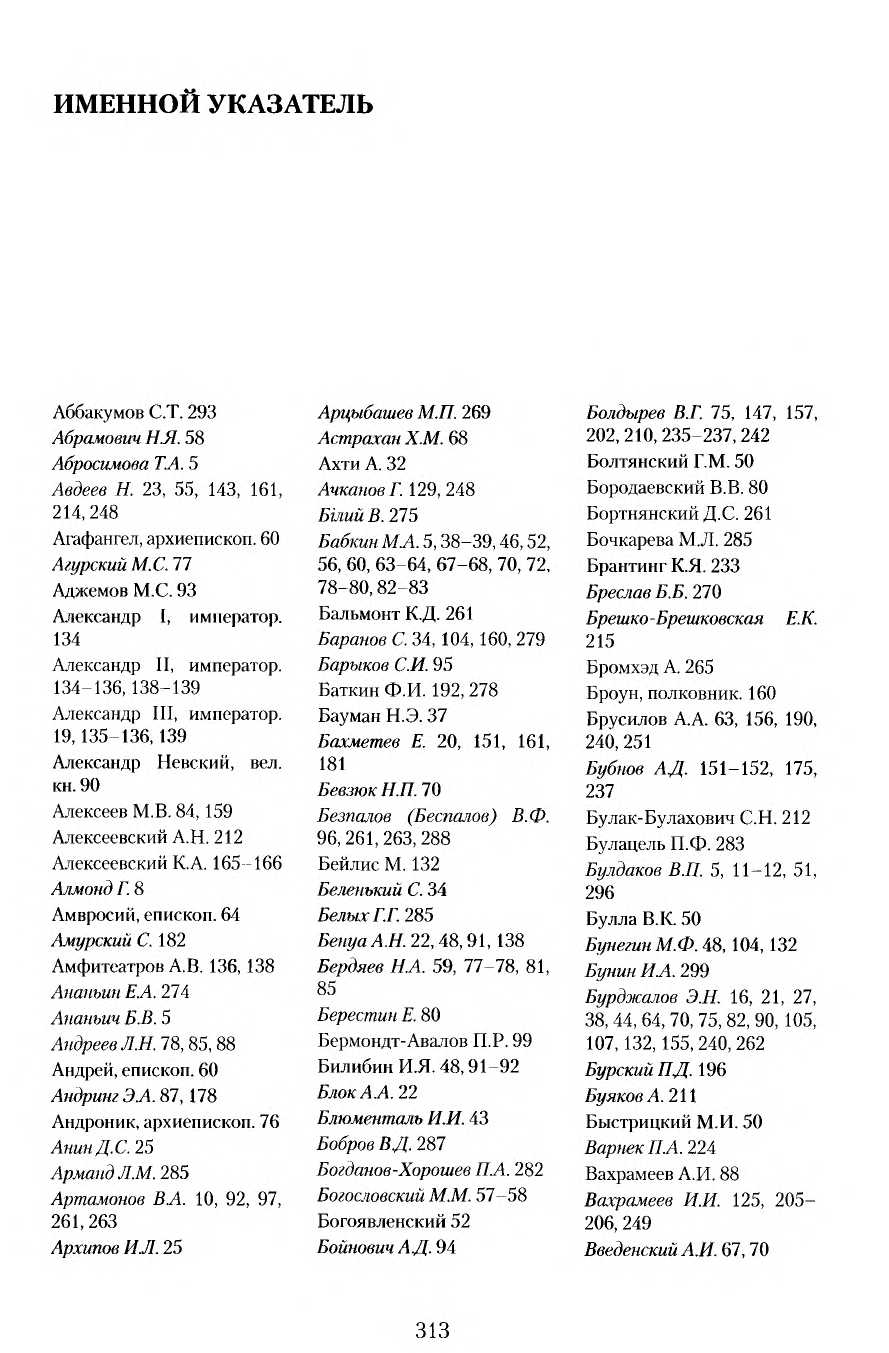
\includegraphics[width=\linewidth,height=229mm,keepaspectratio]{web/assets/index-original-313.png}\par{\small 人名索引（俄文影印），原书第313页。}\clearpage

\hypertarget{name-index-b002}{}% name-index-b002

\clearpage\noindent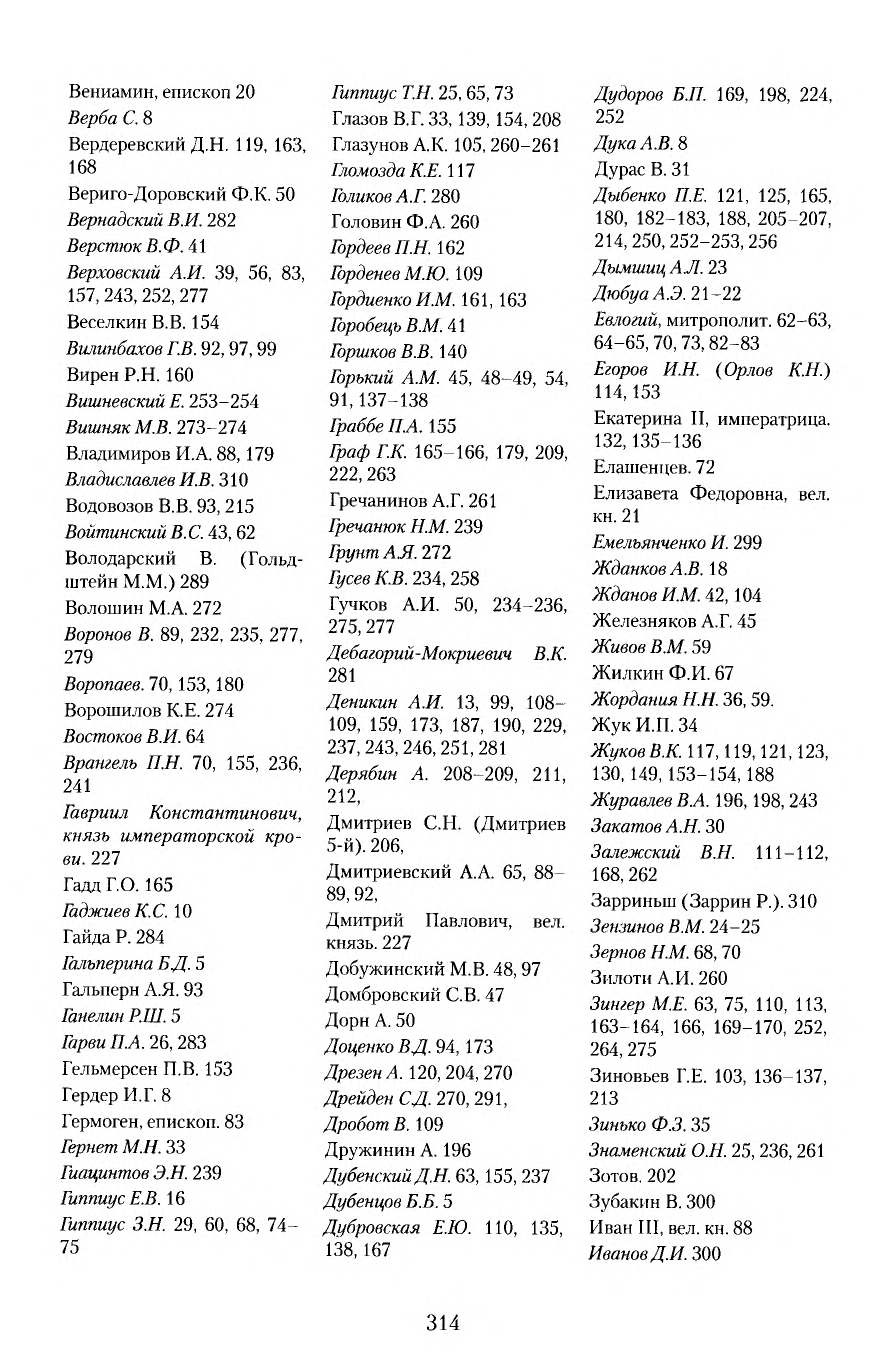
\includegraphics[width=\linewidth,height=229mm,keepaspectratio]{web/assets/index-original-314.png}\par{\small 人名索引（俄文影印），原书第314页。}\clearpage

\hypertarget{name-index-b003}{}% name-index-b003

\clearpage\noindent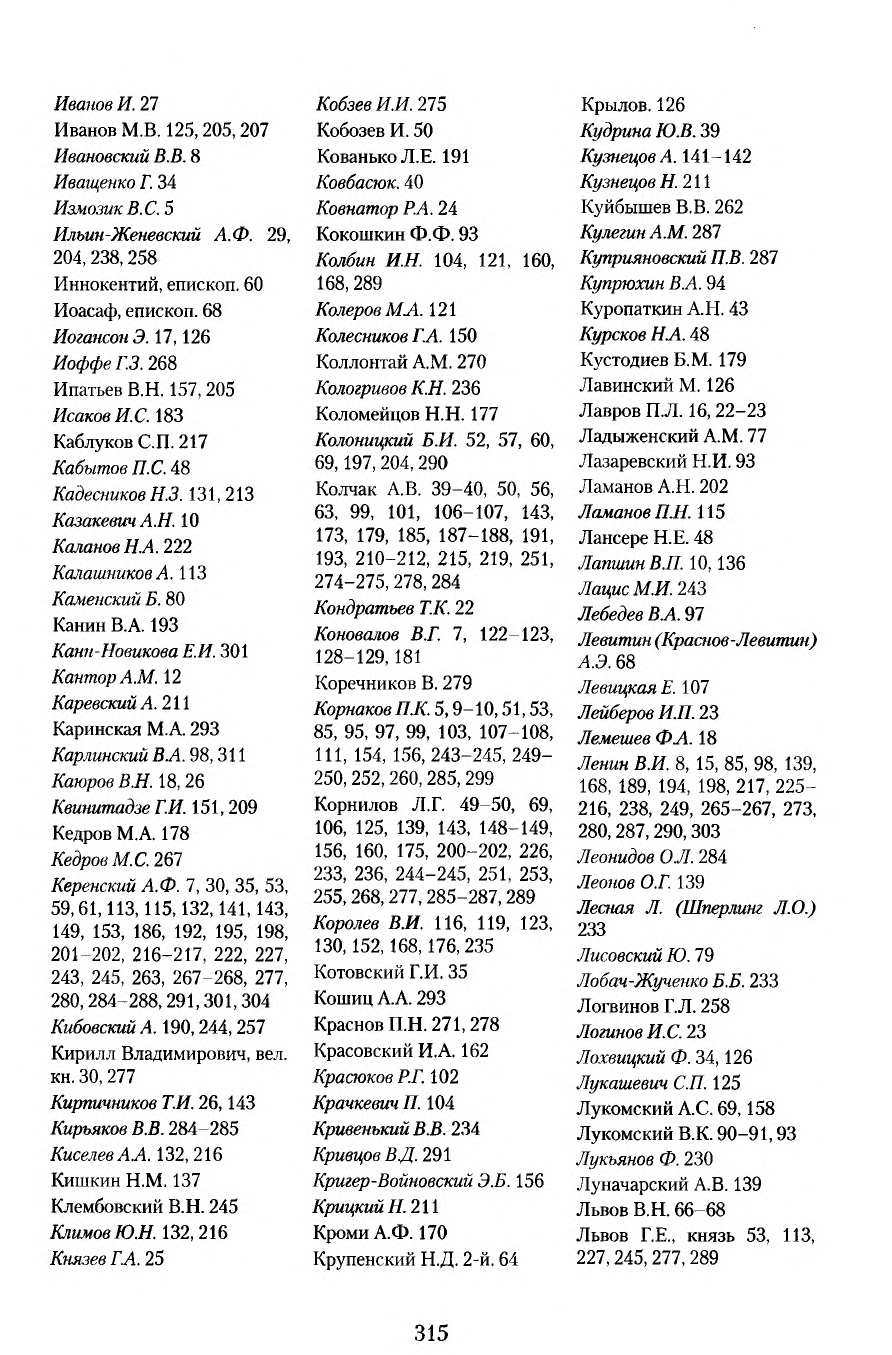
\includegraphics[width=\linewidth,height=229mm,keepaspectratio]{web/assets/index-original-315.png}\par{\small 人名索引（俄文影印），原书第315页。}\clearpage

\hypertarget{name-index-b004}{}% name-index-b004

\clearpage\noindent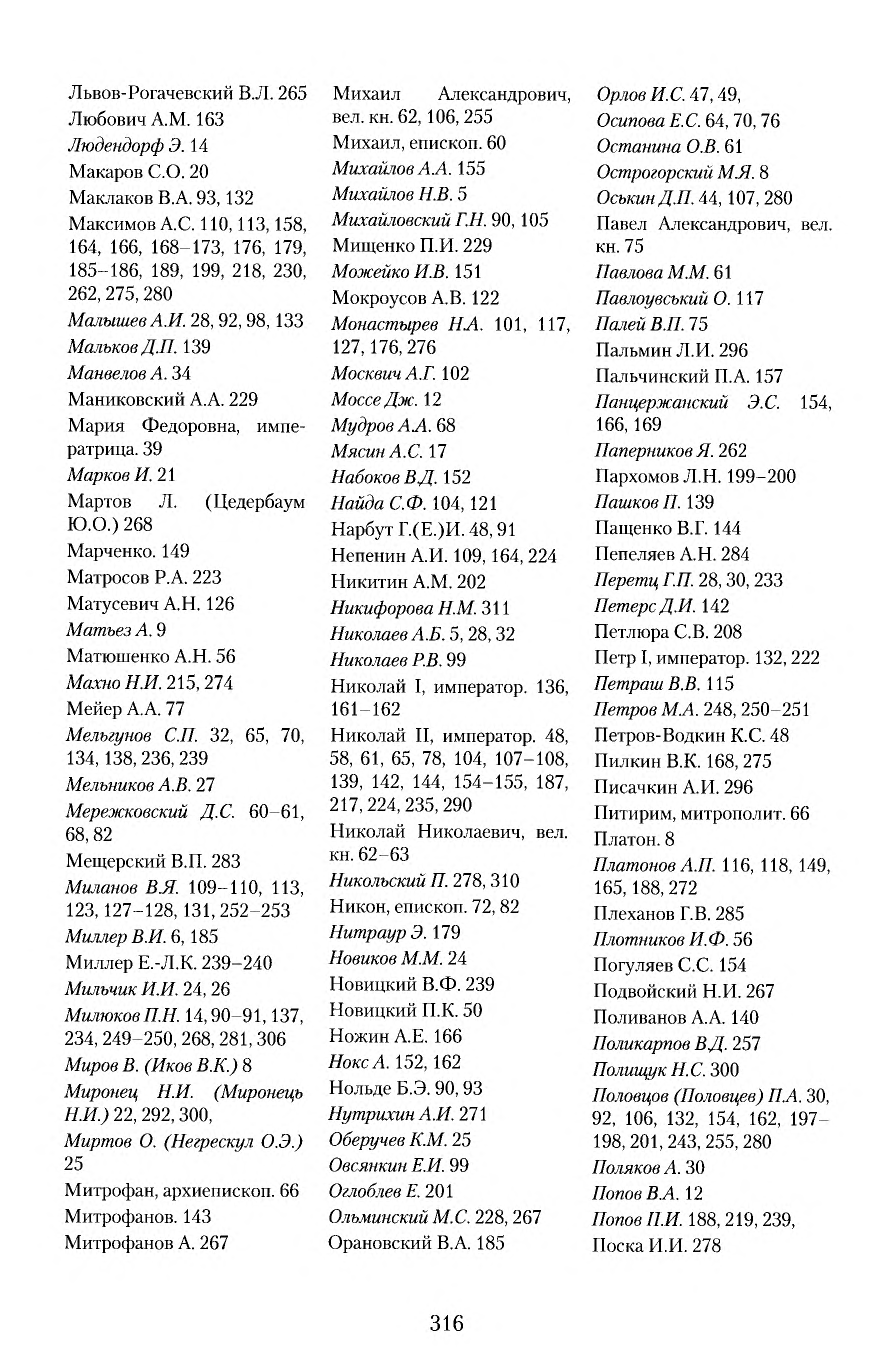
\includegraphics[width=\linewidth,height=229mm,keepaspectratio]{web/assets/index-original-316.png}\par{\small 人名索引（俄文影印），原书第316页。}\clearpage

\hypertarget{name-index-b005}{}% name-index-b005

\clearpage\noindent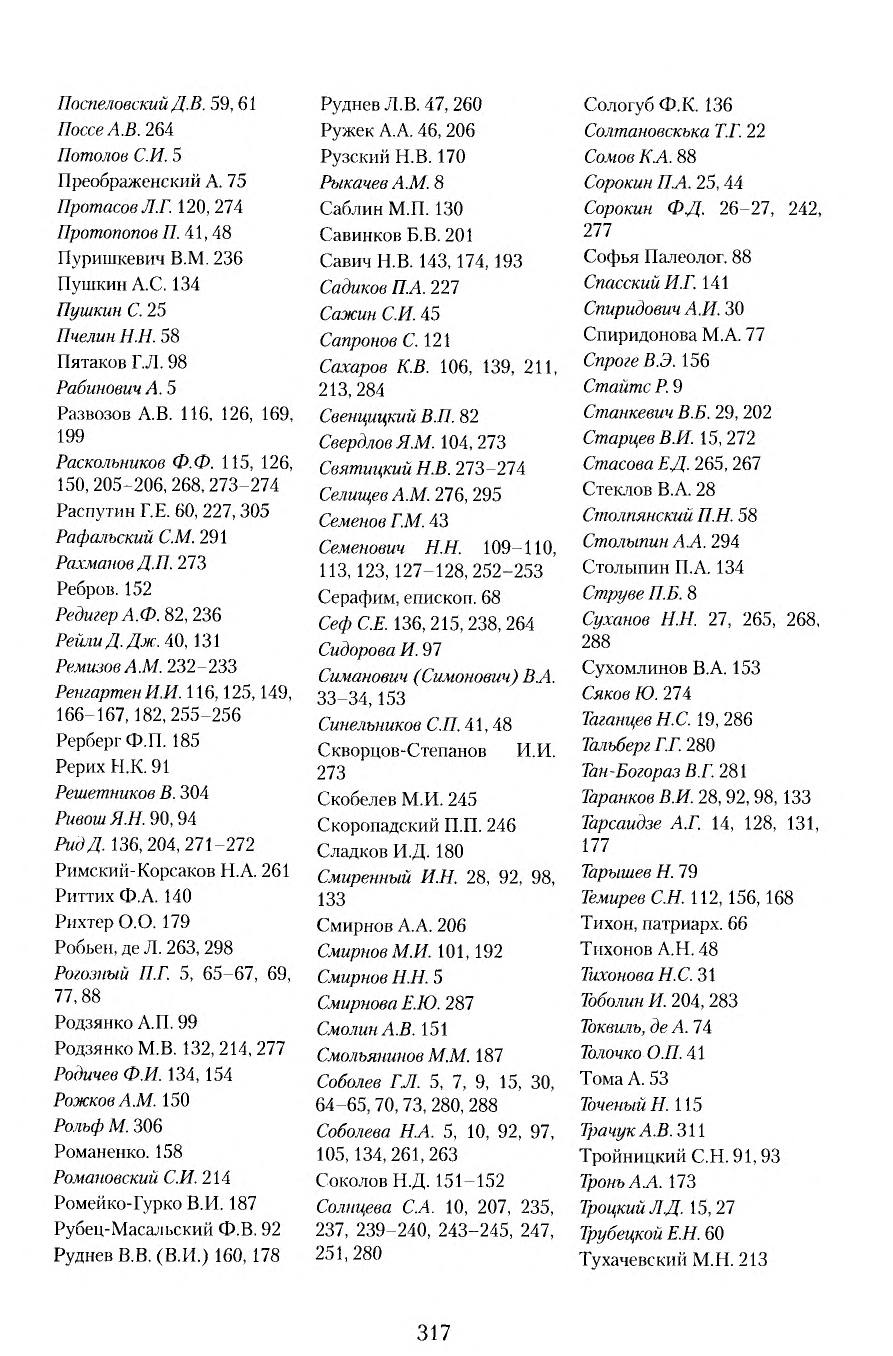
\includegraphics[width=\linewidth,height=229mm,keepaspectratio]{web/assets/index-original-317.png}\par{\small 人名索引（俄文影印），原书第317页。}\clearpage

\hypertarget{name-index-b006}{}% name-index-b006

\clearpage\noindent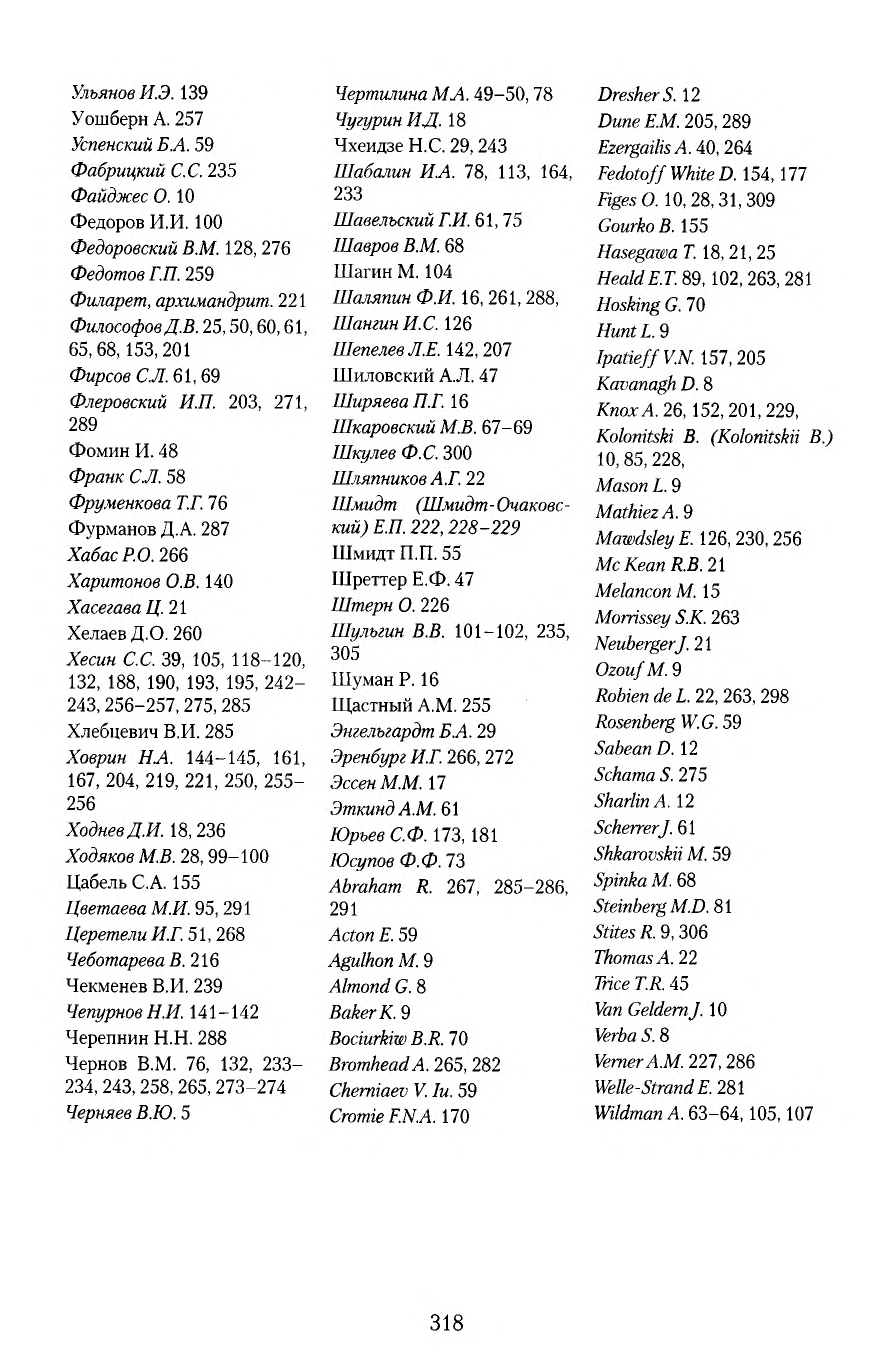
\includegraphics[width=\linewidth,height=229mm,keepaspectratio]{web/assets/index-original-318.png}\par{\small 人名索引（俄文影印），原书第318页。}\clearpage

\chapter{原书出版与印制信息}

\hypertarget{colophon-b001}{}% colophon-b001

信息出版公司“Лики России”
\par


\hypertarget{colophon-b002}{}% colophon-b002

地址：190000, Санкт\babelhyphen{hard}Петербург, пер. Пирогова, 17/8
\par


\hypertarget{colophon-b003}{}% colophon-b003

电话：(812) 312 1121；传真：(812) 320 8788\newline{}
网站：www.liki-rossii.ru
\par


\hypertarget{colophon-b004}{}% colophon-b004

2011年11月10日签付印刷。\newline{}
印张：20＋1（插页；原记“Печ. л. 20+1 вкл.”）。开本：70×100/16。
\par


\hypertarget{colophon-b005}{}% colophon-b005

原书字体：Peterburg C。印数：300册。\newline{}
印制订单号：12-130。
\par


\hypertarget{colophon-b006}{}% colophon-b006

承印：“Сборка”有限责任公司印刷厂。\newline{}
地址：192 077, С.-Петербург, наб. Обводного канала, 64, литера А, корп. 2, пом. 22。\newline{}
电话：(812) 642-43-44。
\par


\chapter{作者与本书简介}

\hypertarget{bio-b001}{}% bio-b001

鲍里斯·伊万诺维奇·科洛尼茨基（1955年生）——历史学博士，俄罗斯科学院圣彼得堡历史研究所主要研究员（ведущий научный сотрудник），圣彼得堡欧洲大学教授。曾在伊利诺伊大学、普林斯顿大学和耶鲁大学担任客座教授。著作有：《解读俄国革命：1917年的语言与象征》（Interpreting the Russian Revolution: The Language and Symbols of 1917. New Haven; London, 1999，与奥兰多·费吉斯（О.Г. Файджес）合著）；《肩章与1917年的权力斗争》（2001）；《象征与权力斗争：1917年俄国革命政治文化研究》（第1版，2001）；《“悲剧的情色”：第一次世界大战时期的皇室形象》（2010）。
\par


\hypertarget{bio-b002}{}% bio-b002

本书考察各种政治象征如何影响1917年政治冲突的产生和进程。书中描述了相互对抗的权力中心和政治力量对民族象征和国家象征、对地下革命运动的象征（旗帜（знамена、флаги）、纹章、国歌与其他颂歌及政治歌曲、国务活动家和政治人物的肖像与纪念碑、勋奖和制服、街道和舰艇名称、人名和姓氏）的态度。同时，本书的任务是重建同时代人赋予这些象征的含义。研究了象征创造的主体和象征传播的渠道（国家机关、政治组织、市场主体）。还考察了政治象征和仪式对大众意识发展、以及对那些未处于政党直接影响下的群众运动自我组织的影响。
\par


\hypertarget{bio-b003}{}% bio-b003

\par\smallskip

\hypertarget{bio-b004}{}% bio-b004

\needspace{164mm}\begin{center}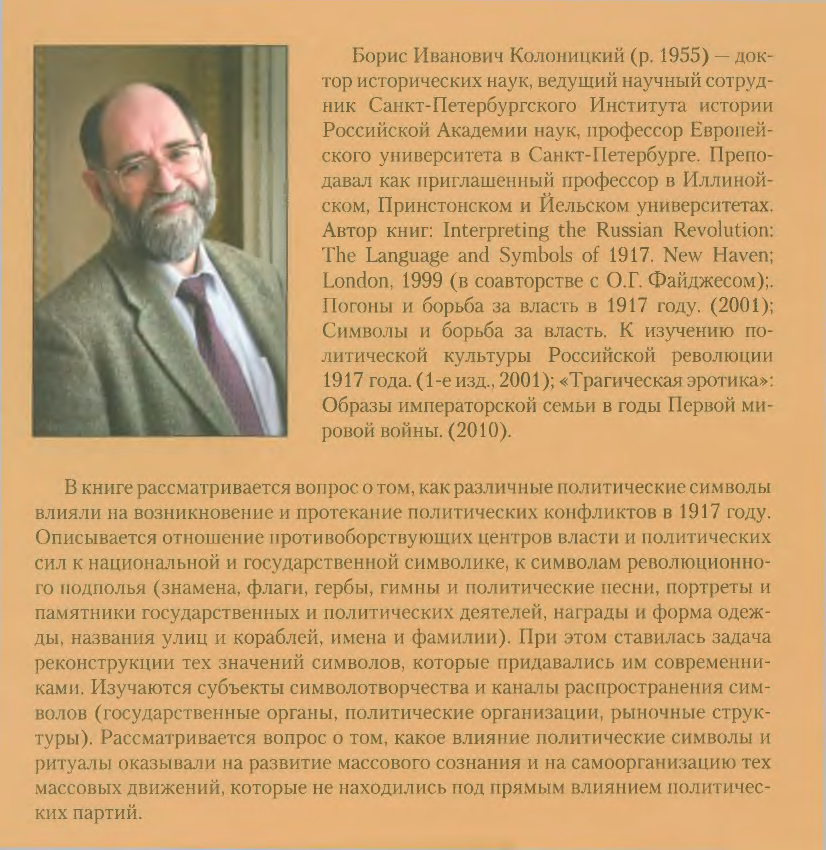
\includegraphics[width=148mm,height=140mm,keepaspectratio]{web/assets/back-cover-source.png}\par{\small 原书封底影印，含作者照片与作者、内容介绍文字}\end{center}

\end{document}
